\documentclass[11pt]{article}

\usepackage[letterpaper,margin=0.84in,headheight=15pt]{geometry}
\usepackage[T1]{fontenc}
\usepackage[utf8]{inputenc}
\usepackage{amsmath,amsthm,amssymb,amscd,mathtools,mathrsfs}
\IfFileExists{newtxtext.sty}{\usepackage{newtxtext,newtxmath}}{\usepackage{lmodern}}
\usepackage{microtype}
\usepackage{booktabs,longtable,tabularx,array,multirow}
\usepackage{enumitem}
\usepackage{graphicx,float,caption,subcaption}
\usepackage{pdflscape}
\usepackage{xcolor}
\usepackage{fancyhdr}
\usepackage{titlesec}
\usepackage{seqsplit}
\usepackage{xurl}
\usepackage[most]{tcolorbox}
\usepackage{hyperref}
\usepackage[nameinlink,capitalise,noabbrev]{cleveref}

\graphicspath{{figures/}}
\allowdisplaybreaks
\setlength{\parindent}{0pt}
\setlength{\parskip}{4.4pt}
\setlist[itemize]{leftmargin=1.65em,itemsep=2pt,topsep=3pt}
\setlist[enumerate]{leftmargin=1.9em,itemsep=2pt,topsep=3pt}
\setcounter{tocdepth}{2}
\setcounter{secnumdepth}{3}

\definecolor{KomorebiNavy}{HTML}{17324D}
\definecolor{KomorebiBlue}{HTML}{3D6C8E}
\definecolor{KomorebiTeal}{HTML}{2F7A78}
\definecolor{KomorebiOrange}{HTML}{B56A2B}
\definecolor{KomorebiRed}{HTML}{9D4B4B}
\definecolor{KomorebiGreen}{HTML}{4F774F}
\definecolor{KomorebiGray}{HTML}{5F6870}
\definecolor{KomorebiPaleBlue}{HTML}{E7F0F6}
\definecolor{KomorebiPaleTeal}{HTML}{E7F2F1}
\definecolor{KomorebiPaleOrange}{HTML}{F7EADF}
\definecolor{KomorebiPaleRed}{HTML}{F5E6E6}
\definecolor{KomorebiPaleGreen}{HTML}{EAF2EA}
\definecolor{KomorebiPaleGray}{HTML}{F1F3F4}

\hypersetup{
  colorlinks=true,
  linkcolor=KomorebiNavy,
  citecolor=KomorebiTeal,
  urlcolor=KomorebiBlue,
  pdfauthor={Komorebi P.},
  pdftitle={Stratified Universality for Resolved Representations},
  pdfsubject={Profiled lane transport, semantic quotient calculus, carrier and observer change, typed obstruction theory, and certified descent},
  pdfkeywords={resolved representation, stratified universality, lane transport, semantic quotient, carrier change, observer base change, task-relative minimality, address holonomy, exact loss, obstruction, certified descent}
}

\pagestyle{fancy}
\fancyhf{}
\fancyhead[L]{\small\textsc{Stratified Universality for Resolved Representations}}
\fancyhead[R]{\small Komorebi P.}
\fancyfoot[C]{\thepage}
\renewcommand{\headrulewidth}{0.4pt}

\titleformat{\section}{\Large\bfseries\color{KomorebiNavy}}{\thesection}{0.7em}{}
\titleformat{\subsection}{\large\bfseries\color{KomorebiNavy}}{\thesubsection}{0.6em}{}
\titleformat{\subsubsection}{\normalsize\bfseries\color{KomorebiNavy}}{\thesubsubsection}{0.5em}{}

\newcolumntype{L}[1]{>{\raggedright\arraybackslash}p{#1}}
\newcolumntype{Y}{>{\raggedright\arraybackslash}X}

\newtheorem{theorem}{Theorem}[section]
\newtheorem{proposition}[theorem]{Proposition}
\newtheorem{lemma}[theorem]{Lemma}
\newtheorem{corollary}[theorem]{Corollary}
\newtheorem{conjecture}[theorem]{Conjecture}
\theoremstyle{definition}
\newtheorem{definition}[theorem]{Definition}
\newtheorem{example}[theorem]{Example}
\newtheorem{construction}[theorem]{Construction}
\theoremstyle{remark}
\newtheorem{remark}[theorem]{Remark}
\newtheorem{boundary}[theorem]{Boundary}

\DeclareMathOperator{\Desc}{Desc}
\DeclareMathOperator{\Core}{Core}
\DeclareMathOperator{\Kar}{Kar}
\DeclareMathOperator{\Add}{Add}
\DeclareMathOperator{\Mod}{Mod}
\DeclareMathOperator{\Fun}{Fun}
\DeclareMathOperator{\Rep}{Rep}
\DeclareMathOperator{\Sem}{Sem}
\DeclareMathOperator{\Fix}{Fix}
\DeclareMathOperator{\coker}{coker}
\DeclareMathOperator{\im}{im}
\DeclareMathOperator{\rank}{rank}
\DeclareMathOperator{\Span}{span}
\DeclareMathOperator{\Gal}{Gal}
\DeclareMathOperator{\Aut}{Aut}
\DeclareMathOperator{\linrank}{linrank}
\DeclareMathOperator{\Hom}{Hom}
\DeclareMathOperator{\End}{End}
\DeclareMathOperator{\Ob}{Ob}
\DeclareMathOperator{\Cone}{Cone}
\DeclareMathOperator{\Hol}{Hol}
\DeclareMathOperator{\Br}{Br}
\DeclareMathOperator{\Reach}{Reach}
\DeclareMathOperator{\Obs}{Obs}
\DeclareMathOperator{\ord}{ord}
\DeclareMathOperator{\Beh}{Beh}
\DeclareMathOperator{\Coim}{Coim}
\DeclareMathOperator{\Ind}{Ind}
\DeclareMathOperator{\Def}{Def}
\DeclareMathOperator{\Cl}{Cl}
\DeclareMathOperator{\Rel}{Rel}
\DeclareMathOperator{\kerpair}{KerPair}
\newcommand{\Cat}{\mathbf{Cat}}
\newcommand{\Gpd}{\mathbf{Gpd}}
\newcommand{\Seq}{\mathbf{Seq}}
\newcommand{\Rat}{\mathbf{Rat}}
\newcommand{\Rec}{\mathbf{Rec}}
\newcommand{\State}{\mathbf{State}}
\newcommand{\Per}{\mathbf{Per}}
\newcommand{\Mask}{\mathbf{Mask}}
\newcommand{\RMah}{\mathbf{RMah}}
\newcommand{\Reg}{\mathbf{Reg}}
\newcommand{\DFAO}{\mathbf{DFAO}}
\newcommand{\bbK}{\mathbb K}
\newcommand{\kk}{\Bbbk}
\newcommand{\id}{\mathrm{id}}
\newcommand{\Syn}{\operatorname{Syn}}
\newcommand{\Analysis}{\mathcal A}
\newcommand{\Synthesis}{\mathcal S}

\newcommand{\statuspill}[3]{%
  \begingroup\setlength{\fboxsep}{2.1pt}%
  \colorbox{#1}{\textcolor{#2}{\strut\scriptsize\sffamily #3}}%
  \endgroup}
\newcommand{\StatusInternal}{\statuspill{KomorebiPaleGreen}{KomorebiGreen}{proved internally}}
\newcommand{\StatusConditional}{\statuspill{KomorebiPaleOrange}{KomorebiOrange}{proved conditionally}}
\newcommand{\StatusClassical}{\statuspill{KomorebiPaleBlue}{KomorebiBlue}{classical input}}
\newcommand{\StatusComputed}{\statuspill{KomorebiPaleTeal}{KomorebiTeal}{computed exactly}}
\newcommand{\StatusFramework}{\statuspill{KomorebiPaleGray}{KomorebiGray}{framework only}}
\newcommand{\StatusConjectural}{\statuspill{KomorebiPaleRed}{KomorebiRed}{conjectural}}
\newcommand{\StatusSuperseded}{\statuspill{KomorebiPaleGray}{KomorebiGray}{superseded}}
\newcommand{\StatusExternal}{\statuspill{KomorebiPaleBlue}{KomorebiNavy}{externally reviewed}}

\newtcolorbox{claimbox}[1][]{
  enhanced,breakable,colback=KomorebiPaleBlue,colframe=KomorebiNavy,
  boxrule=0.8pt,arc=1.5mm,left=2.5mm,right=2.5mm,top=2mm,bottom=2mm,#1}
\newtcolorbox{boundarybox}[1][]{
  enhanced,breakable,colback=KomorebiPaleRed,colframe=KomorebiRed,
  boxrule=0.8pt,arc=1.5mm,left=2.5mm,right=2.5mm,top=2mm,bottom=2mm,#1}
\newtcolorbox{resultbox}[1][]{
  enhanced,breakable,colback=KomorebiPaleGreen,colframe=KomorebiGreen,
  boxrule=0.8pt,arc=1.5mm,left=2.5mm,right=2.5mm,top=2mm,bottom=2mm,#1}

\newtcolorbox{ConcordanceEntry}[3]{
  enhanced,breakable,colback=white,colframe=KomorebiBlue,
  boxrule=0.55pt,arc=1mm,left=2mm,right=2mm,top=1.5mm,bottom=1.5mm,
  title={\texttt{#1}\quad #2\hfill #3},
  fonttitle=\small\bfseries,coltitle=KomorebiNavy,colbacktitle=KomorebiPaleBlue,
  attach boxed title to top left={xshift=0mm,yshift=-0.5mm},
  boxed title style={boxrule=0pt,arc=0.8mm,left=1.5mm,right=1.5mm,top=1mm,bottom=1mm}}
\newcommand{\ConcordanceField}[2]{\par\noindent\textbf{#1.} #2}

\crefname{theorem}{theorem}{theorems}
\crefname{proposition}{proposition}{propositions}
\crefname{lemma}{lemma}{lemmas}
\crefname{corollary}{corollary}{corollaries}
\crefname{definition}{definition}{definitions}
\crefname{example}{example}{examples}
\crefname{construction}{construction}{constructions}
\crefname{remark}{remark}{remarks}
\crefname{boundary}{boundary}{boundaries}

\newcommand{\BlockThirteenBridgeChecks}{154,209}
\newcommand{\BlockThirteenInvariantChecks}{119,453}
\newcommand{\BlockThirteenRegressionChecks}{39,846}
\newcommand{\BlockThirteenNewChecks}{233,816}
\newcommand{\BlockThirteenChecks}{273,662}
\newcommand{\BlockThirteenCumulative}{2,272,676}
\newcommand{\BlockThirteenCumulativeExecuted}{2,312,522}

\newcommand{\BlockFourteenAuditChecks}{41}
\newcommand{\BlockFourteenAuditFailures}{0}
\newcommand{\BlockFourteenAbstractWords}{240}
\newcommand{\BlockFourteenSourceFiles}{51}
\newcommand{\BlockFourteenLabels}{477}
\newcommand{\BlockFourteenReferences}{124}

\IfFileExists{generated/block15_counts.tex}{\newcommand{\BlockFifteenValidationAssertions}{197,099}
\newcommand{\BlockFifteenValidationFailures}{0}
\newcommand{\BlockFifteenLaneAssertions}{197,099}
\newcommand{\BlockFifteenLaneFailures}{0}
\newcommand{\BlockFifteenIntegerMatrixAssertions}{28,490}
\newcommand{\BlockFifteenRationalRefinementAssertions}{16,674}
\newcommand{\BlockFifteenFoldAssertions}{1,000}
\newcommand{\BlockFifteenSupportAssertions}{300}
\newcommand{\BlockFifteenFactorialAssertions}{150,630}
\newcommand{\BlockFifteenNegativeControlAssertions}{5}
}{}
\IfFileExists{generated/block15_publication_counts.tex}{\newcommand{\BlockFifteenAuditChecks}{77}
\newcommand{\BlockFifteenAuditFailures}{0}
\newcommand{\BlockFifteenAbstractWords}{316}
\newcommand{\BlockFifteenSourceFiles}{55}
\newcommand{\BlockFifteenLabels}{519}
\newcommand{\BlockFifteenReferences}{131}
}{}
\IfFileExists{generated/block16_counts.tex}{% Generated by verify_block16_holonomy_lane_transport.py
\newcommand{\BlockSixteenValidationAssertions}{1,344,823}
\newcommand{\BlockSixteenValidationFailures}{0}
}{}
\IfFileExists{generated/block16_publication_counts.tex}{% Generated by verify_block16_publication_audit.py
\newcommand{\BlockSixteenAuditChecks}{85}
\newcommand{\BlockSixteenAuditFailures}{0}
\newcommand{\BlockSixteenAbstractWords}{346}
\newcommand{\BlockSixteenSourceFiles}{60}
\newcommand{\BlockSixteenLabels}{542}
\newcommand{\BlockSixteenReferences}{138}
}{}
\IfFileExists{generated/block17_counts.tex}{% Generated by verify_block17_semantic_extension.py
\newcommand{\BlockSeventeenValidationAssertions}{3,022}
\newcommand{\BlockSeventeenValidationFailures}{0}
\newcommand{\BlockSeventeenSemanticTrials}{1,000}
}{}

\begin{document}

\hypersetup{pageanchor=false}
\begin{titlepage}
\centering
\vspace*{0.42in}
{\small\sffamily\bfseries\color{KomorebiBlue} KOMOREBI MATH}\par
\vspace{0.20in}
{\Huge\bfseries\color{KomorebiNavy} Stratified Universality for Resolved Representations\par}
\vspace{0.16in}
{\Large Profiled Lane Transport, Semantic Quotients, Carrier Change, and Certified Descent\par}
\vspace{0.10in}
{\large\color{KomorebiBlue} Final Formal Foundations Edition\par}
\vspace{0.38in}
{\Large Komorebi P.\par}
\vspace{0.10in}
{\large 23 September 2026\par}
\vspace{0.25in}
\begin{tcolorbox}[width=0.88\textwidth,colback=KomorebiPaleGray,colframe=KomorebiGray,boxrule=0.7pt,arc=1mm]
\centering\small
\textbf{Version 2.0.0.} This edition preserves the verified finite atlas and finite profiled and holonomy-twisted lane theorems, then adds a formal calculus of task-relative semantic quotients, exact bridge loss, carrier factorization, observer base change, admissibility-relative obstruction, and enrichment lifting. Inherited claims retain their original proof boundaries. New claims are separated in Part IV and in the expanded theorem concordance.
\end{tcolorbox}
\vfill
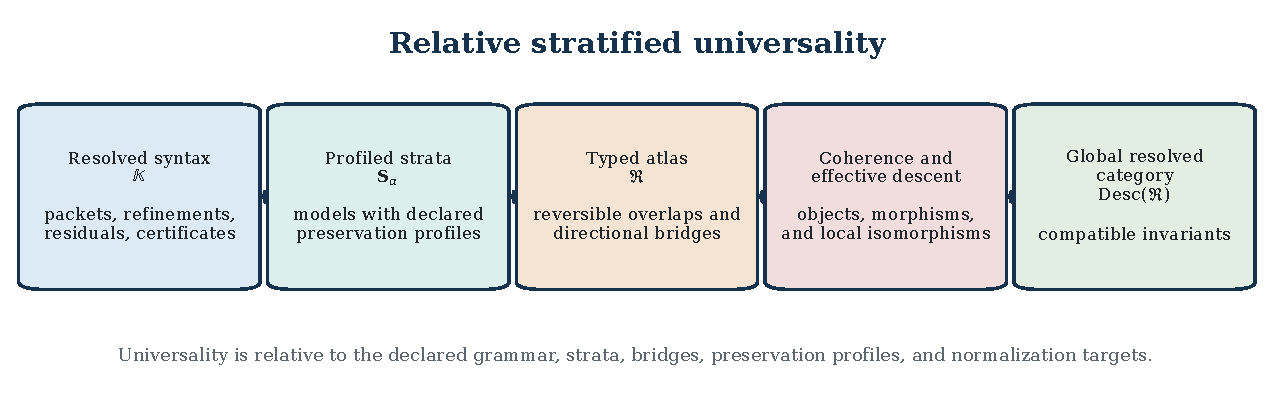
\includegraphics[width=0.96\textwidth]{architecture.pdf}
\vfill
{\small\color{KomorebiGray}
Universality is asserted only relative to declared grammars, strata, bridges, preservation profiles, normalization targets, and descent doctrines.}
\end{titlepage}
\hypersetup{pageanchor=true}

\pagenumbering{roman}
\thispagestyle{plain}
\begin{abstract}
Komorebi Math is formulated as a relative classifying and transport theory of resolved representations. A resolved theory records typed operations, packet decompositions, refinement laws, residuals, certificates, and only those analytic, tensor, metric, or arithmetic structures included in a declared preservation profile. Its realizations are organized into normalized strata. Reversible changes of presentation form representation groupoids, while quotients, completions, reductions, and other information-losing constructions remain in a directed category with explicit loss passports.

The first theorem layer establishes the additive--Karoubi resolved envelope, finite profiled atlas assembly, and componentwise invariant descent. The finite profiled Universal Lane Transport Theorem identifies every morphism between complete finite split packet systems with its full lane matrix. Composition becomes block contraction, refinement is functorial, and selectors split retained transport from a named residual. Under finite address holonomy, the same calculus descends as sections of a matrix local system. Monodromy orbits give the finest ordinary global lane coarsening, and pair orbits carry the compatible selector algebra.

The second theorem layer formalizes task-relative semantics. For a declared continuation grammar and observation family, the behavioral quotient is the coarsest exact representation preserving every future observation. In module-valued slices, task combination, common coarsening, relative residuals, bridge loss, essential-image failure, and task weakening fit into canonical exact sequences. Carrier replacement is possible exactly on a kernel-factorization locus. Set-valued residual equality and linear residual span are separated by an explicit relation module. Convex value packets, provenance states, additive route packets, and weighted-linear states therefore remain distinct unless certified comparison maps are supplied.

Finally, obstruction is indexed by the admissible realization class. Enlarging that class can reduce an optimized defect, while zero infimum may still fail to be attained. Rich structure descends under forgetting, but reconstructing it from a bare bridge is a typed lifting problem. The resulting theory is finite, profiled, task-relative, and auditable. It does not assert one global coordinate system, one observer-independent minimum, equivalence of all carriers, or effectivity of an unrestricted heterogeneous stack.
\end{abstract}

\begin{center}
\small\textbf{Keywords:} resolved representation, stratified universality, lane transport, semantic quotient, behavioral core, carrier change, observer base change, exact loss, address holonomy, admissibility-relative obstruction, certified descent.
\end{center}

\begin{claimbox}
\textbf{Central claim.}
Komorebi Math is a stratified classifying and transport theory of resolved representations. Within a declared profile, it separates exact representation change from directional information loss. Within a declared semantic slice, it constructs the coarsest representation preserving all future task observations. Changes of carrier, observer, geometry, completion, or enrichment are legal only through certified comparison or lifting data.
\end{claimbox}

\begin{boundarybox}
\textbf{Claim boundary.}
The paper does not assert that every mathematical object has a finite Komorebi presentation, that all strata or carriers are equivalent, that every bridge is reversible, that arbitrary presentations admit one observer-independent minimum, or that the unrestricted heterogeneous atlas is an effective stack. Internal proof status, exact computation, classical import, historical novelty, and independent peer validation remain distinct classifications.
\end{boundarybox}

\tableofcontents
\clearpage
\pagenumbering{arabic}

\section{Introduction}

\subsection{The assembly problem}

The source manuscripts already contain typed quiver and module semantics, seed presentations, exact packet coordinates, refinement and residual calculus, nonlinear packet composition, finite holonomy, relative obstruction objects, operator-algebraic recognition, Galois descent, and several exact sequence and arithmetic realizations \cite{P1,RT,P3,GAL,SEQ}. The central problem is therefore no longer to reconstruct these foundations independently. It is to determine when they assemble into one finite, typed, coherent classifying object.

The proposed architecture has six layers:
\[
\boxed{
\begin{gathered}
\text{resolved syntax}\longrightarrow\text{normalized strata}
\longrightarrow\text{typed overlaps}\longrightarrow\text{coherence}\cr
\longrightarrow\text{effective descent}
\longrightarrow\text{compatible complete invariants}.
\end{gathered}}
\]
Each arrow carries a proof obligation. A semantic analogy is not a bridge. A bridge is not reversible merely because formulas exist in both directions. Local completeness is not global completeness until the local isomorphisms themselves satisfy descent.

\subsection{Main theorem and classification domain}

Three theorem levels are kept distinct. First, the finite profiled Universal Lane Transport Theorem is an internal theorem about complete finite split packet systems in an additive idempotent-complete category. Its holonomy-twisted extension retains exact analysis, synthesis, composition, refinement, selectors, and residuals when chart loops permute lane addresses. The global coordinate object is then a matrix local system, and ordinary lane projectors descend at the monodromy-orbit resolution.

Second, the finite atlas assembly theorem is conditional in general. Given profile-preserving normalized strata, typed reversible overlaps, coherent comparison cells, effective descent, and compatible native invariants, the descended invariant reflects isomorphism. The manuscript verifies these hypotheses on a finite certified atlas whose reversible core has five connected semantic components.

Third, the semantic quotient theorem works inside a fixed doctrine and declared observation category. It constructs the maximal continuation-stable invisible core and the associated task-relative quotient. In module-valued slices, semantic combination and bridge transport admit canonical exact sequences. Carrier and observer changes are separate factorization problems, while changes of admissible geometry or enrichment are typed lifting problems.

The statements are strongest precisely because their targets are explicit. Lane transport concerns declared finite resolutions. Atlas classification concerns the declared normalized finite atlas. Behavioral minimality concerns one semantic slice. None of these statements classifies arbitrary presentations, identifies all carrier algebras, or promotes unverified doctrine changes to equivalences.

\subsection{Contributions}

The paper makes fourteen consolidated contributions.
\begin{enumerate}
\item It provides a source-controlled theorem concordance and an explicit profile-indexed additive--Karoubi resolved envelope.
\item It separates representation groupoids from the directed transformation category and assigns every certified bridge a preservation and information-loss passport.
\item It proves a finite profiled atlas assembly theorem and distinguishes holonomy, relative cokernel, Brauer, and higher-coherence defects.
\item It establishes normalized effective-descent atlases and complete native invariants on the five-component certified semantic union.
\item It proves exact bridge comparison and higher coherence, including the nonlinear--algebraic--holonomic Fuss--Catalan triangle.
\item It proves the finite profiled Universal Lane Transport Theorem with exact block transport, refinement, selectors, residuals, and separately typed fold and kernel clauses.
\item It removes the trivial-address-holonomy restriction from transport by proving matrix-local-system descent, orbit coarsening, pair-orbit selectors, and orbital path composition.
\item It defines the task-relative behavioral quotient as the coarsest exact representation preserving all declared future observations.
\item It identifies the behavioral kernel as the maximal continuation-stable invisible core and gives a greatest-fixed-point computation with finite-dimensional termination.
\item It proves the semantic diamond, relative semantic residual, task-change exact sequence, bridge-loss exact sequence, and extension law for composite loss in module-valued slices.
\item It proves the carrier factorization gate and the universal joint completion preserving two incomparable carrier semantics.
\item It separates Set-valued continuation minimization from linear residual minimization by an exact relation-module sequence and an explicit polyphase family with infinite discrete state and finite Hankel rank.
\item It proves carrier-indexed observer aggregation and observer-conditioned convex packet transport, while isolating cancellation, idempotence, singular-resurrection, and provenance boundaries.
\item It formalizes admissibility monotonicity, completion/gap/escape stratification, a sharp convex-versus-quadratic example, and the forgetful-descent versus enrichment-lifting principle.
\end{enumerate}

\subsection{Proof status and organization}

Classical inputs, internally proved theorems, exact finite verification, conditional statements, framework definitions, and conjectures are separately marked. The theorem concordance is source control for this distinction. Part I gives the common resolved foundation and finite assembly theorem. Part II develops the certified native strata. Part III gives global synthesis and finite profiled and holonomy-twisted lane transport. Part IV develops task-relative semantic quotients, carrier and observer change, exact loss, admissibility-relative obstruction, and doctrine lifting. The final sections state scope and conclusion. Detailed development, claim-boundary, and validation records are retained in the appendices.

\section{Main theorem suite and proof architecture}
\label{sec:block14-main-suite}

Let
\[
 \mathfrak A_{\mathrm{cert}}:=\mathfrak A_{13}
\]
denote the finite certified atlas constructed in \cref{sec:block13-global-invariant}.  Its reversible core is the disjoint union of five connected semantic components, while its directional satellites retain explicit loss or obstruction passports.

\begin{theorem}[Stratified resolved representation, descent, and complete invariant theorem]
\label{thm:block14-main}
Let \(\mathbb K\) be the resolved theory used in this manuscript and let \(\mathfrak A_{\mathrm{cert}}\) be the declared finite atlas.  Then the following statements hold.
\begin{enumerate}
\item Every chart is a profile-preserving realization of the common resolved syntax, and every reversible edge is an equivalence on its named overlap category.
\item The descent category exists as the finite pseudolimit of the atlas and decomposes as the coproduct of its five connected semantic components.
\item Every proof whose constructor support lies in the common verified preservation profile transports to compatible local theorems and hence to the corresponding global resolved object.
\item The semantic normalizers induce the comparison 2-cells on all nonempty triple overlaps and force the quadruple-overlap coherence equation.
\item The compatible native invariant family descends to a tagged global invariant
\[
 \mathcal J_{\mathrm{cert}}:
 \Desc(\mathfrak A_{\mathrm{cert}})
 \longrightarrow
 \Desc(\mathcal V_{\mathrm{cert}}).
\]
\item The descended invariant is complete on the declared normalized global category:
\[
 \mathcal J_{\mathrm{cert}}(X)\cong
 \mathcal J_{\mathrm{cert}}(Y)
 \quad\Longleftrightarrow\quad
 X\cong Y.
\]
\item Every noninvertible construction remains outside the reversible core and carries a typed record of its preserved structure, forgotten information, named residual, or obstruction class.
\end{enumerate}
\end{theorem}

\begin{proof}
The common resolved syntax and preservation-profile transport are established in \cref{sec:resolved-foundations}.  The finite atlas and its pseudolimit are supplied by \cref{thm:atlas-assembly}.  The normalizer comparison cells and their higher coherence are \cref{thm:block13-normalizer-coherence}.  Descent of compatible invariant families is \cref{thm:block13-certified-invariant-descent}.  Completeness is \cref{thm:block13-global-completeness}; its hypotheses are verified component by component in \cref{sec:block13-global-invariant}.  The bridge passports and obstruction taxonomy in \cref{sec:strata-bridges-obstructions} keep every directional construction outside the maximal subgroupoid.  Combining these results proves all seven assertions.
\end{proof}

\begin{corollary}[Relative universality]
\label{cor:block14-relative-universality}
The certified atlas is universal for profile-preserving models of the declared resolved grammar on its five normalized semantic components.  This universality is relative to the chosen grammar, strata, bridges, preservation profiles, normalization targets, and descent doctrine.
\end{corollary}

\begin{theorem}[Relative semantic quotient and typed contract-change theorem]
\label{thm:block17-main-semantic}
Fix a declared semantic slice in a stratum of the resolved theory.  Assume the required effective quotients exist.  Then:
\begin{enumerate}
\item the behavioral quotient is the coarsest exact representation preserving all declared future observations;
\item its kernel or congruence is the maximal continuation-stable invisible core;
\item strengthening the task induces a canonical map from the stronger quotient to the weaker quotient;
\item in module-valued slices, joint semantics, shared semantics, relative residuals, bridge loss, essential-image failure, and task weakening fit into canonical exact sequences;
\item one carrier semantics replaces another exactly on the corresponding kernel-factorization locus;
\item observer base change may introduce an independent relation object and therefore does not follow from carrier compatibility;
\item enlarging an admissible realization class can only decrease optimized defect, but zero infimum need not be attained;
\item lifting a bare bridge to richer metric, tensor, topological, projective, or completed structure requires a separate enhancement certificate.
\end{enumerate}
\end{theorem}

\begin{proof}
The universal quotient and maximal-core statements are \cref{thm:block17-universal-behavioral-coimage,thm:block17-behavioral-core}.  Task change and the module exact sequences are \cref{thm:block17-task-change,thm:block17-semantic-diamond,thm:block18-bridge-loss-exact,thm:block18-loss-composition}.  Carrier and observer change are \cref{thm:block18-carrier-factorization,thm:block18-observer-base-change}.  Admissibility monotonicity is \cref{thm:block19-admissibility-monotonicity}, and the enrichment statement is \cref{prop:block19-forgetful-lifting}.  Each assertion retains its printed doctrine and existence hypotheses.
\end{proof}

\begin{corollary}[No absolute minimal representation]
\label{cor:block17-no-absolute-minimum}
There is no observer-independent or doctrine-independent minimum asserted by this manuscript.  Minimality is relative to the carrier, continuation grammar, observation category, query family, and admissible enrichment class.
\end{corollary}

\begin{boundary}[Publication boundary]
\label{bnd:block14-publication-boundary}
\Cref{thm:block14-main} does not imply a global canonical normal form for arbitrary mathematical objects, equivalence of all broad strata, decidability of arbitrary presentation equivalence, or effectivity of an unrestricted heterogeneous stack.  It also does not identify functional-Mahler equations with Newton-Mahler interpolation, forget branch data in the algebraic-to-holonomic direction, or infer Tannakian symmetry from a merely faithful additive realization.
\end{boundary}

\begin{table}[htbp]
\centering
\small
\caption{The publication theorem spine.  Section numbers are resolved by the final build; the logical order, rather than the numbering, is authoritative.}
\label{tab:block14-theorem-suite}
\begin{tabularx}{\textwidth}{@{}L{0.16\textwidth}L{0.22\textwidth}YL{0.14\textwidth}@{}}
\toprule
Stage & Principal result & Exact role in the proof & Location \\
\midrule
Resolved source & Additive-Karoubi envelope & Literal finite packet objects and profile-indexed realization source & \cref{thm:additive-karoubi-envelope} \\
Typed atlas & Bridge passports and obstruction separation & Reversible overlaps are separated from directional loss & \cref{sec:strata-bridges-obstructions} \\
Finite assembly & Profiled atlas assembly & Bilimit, theorem transport, groupoid core, and global directional functors & \cref{thm:atlas-assembly} \\
Native normalization & Certified stratum atlases & Complete local coordinates on declared semantic slices & Part II \\
Higher coherence & Normalizer-induced coherence & Unique semantic normalizers force all certified overlap cycles to commute & \cref{thm:block13-normalizer-coherence} \\
Invariant descent & Certified invariant-descent theorem & Coherent local invariants descend through effective object and morphism gluing & \cref{thm:block13-certified-invariant-descent} \\
Global completeness & Tagged componentwise invariant & The descended invariant reflects isomorphism on the five-component union & \cref{thm:block13-global-completeness,thm:block14-main} \\
Lane transport & Finite profiled Universal Lane Transport Theorem & Exact block transport, refinement, selection, residuals, conditional fold loss, and certified descent & \cref{thm:block15-universal-lane-transport,thm:block15-lane-descent} \\
Twisted transport & Holonomy-Twisted Universal Lane Transport Theorem & Matrix-local-system synthesis, base-fiber invariant normal form, orbit coarsening, and orbital path algebra & \cref{thm:block16-holonomy-twisted-lane-transport,cor:block16-base-fiber-invariant-normal-form,thm:block16-orbit-descent,thm:block16-permutation-orbital-calculus} \\
Task semantics & Relative semantic quotient theorem & Behavioral cores, task quotients, semantic diamonds, and exact task loss & \cref{thm:block17-main-semantic,thm:block17-semantic-diamond,thm:block17-task-change} \\
Carrier and observer change & Factorization and base-change theorems & Joint semantic completion, exact bridge loss, relation modules, and carrier-indexed aggregation & \cref{thm:block18-carrier-factorization,thm:block18-bridge-loss-exact,thm:block18-observer-base-change,thm:block18-carrier-indexed-observer} \\
Admissibility and lifting & Class-relative defect and enhancement gates & Completion/gap/escape, geometry-class separation, and typed enrichment lifting & \cref{thm:block19-admissibility-monotonicity,thm:block19-convex-quadratic-separation,prop:block19-forgetful-lifting} \\
\bottomrule
\end{tabularx}
\end{table}


\begin{figure}[htbp]
\centering
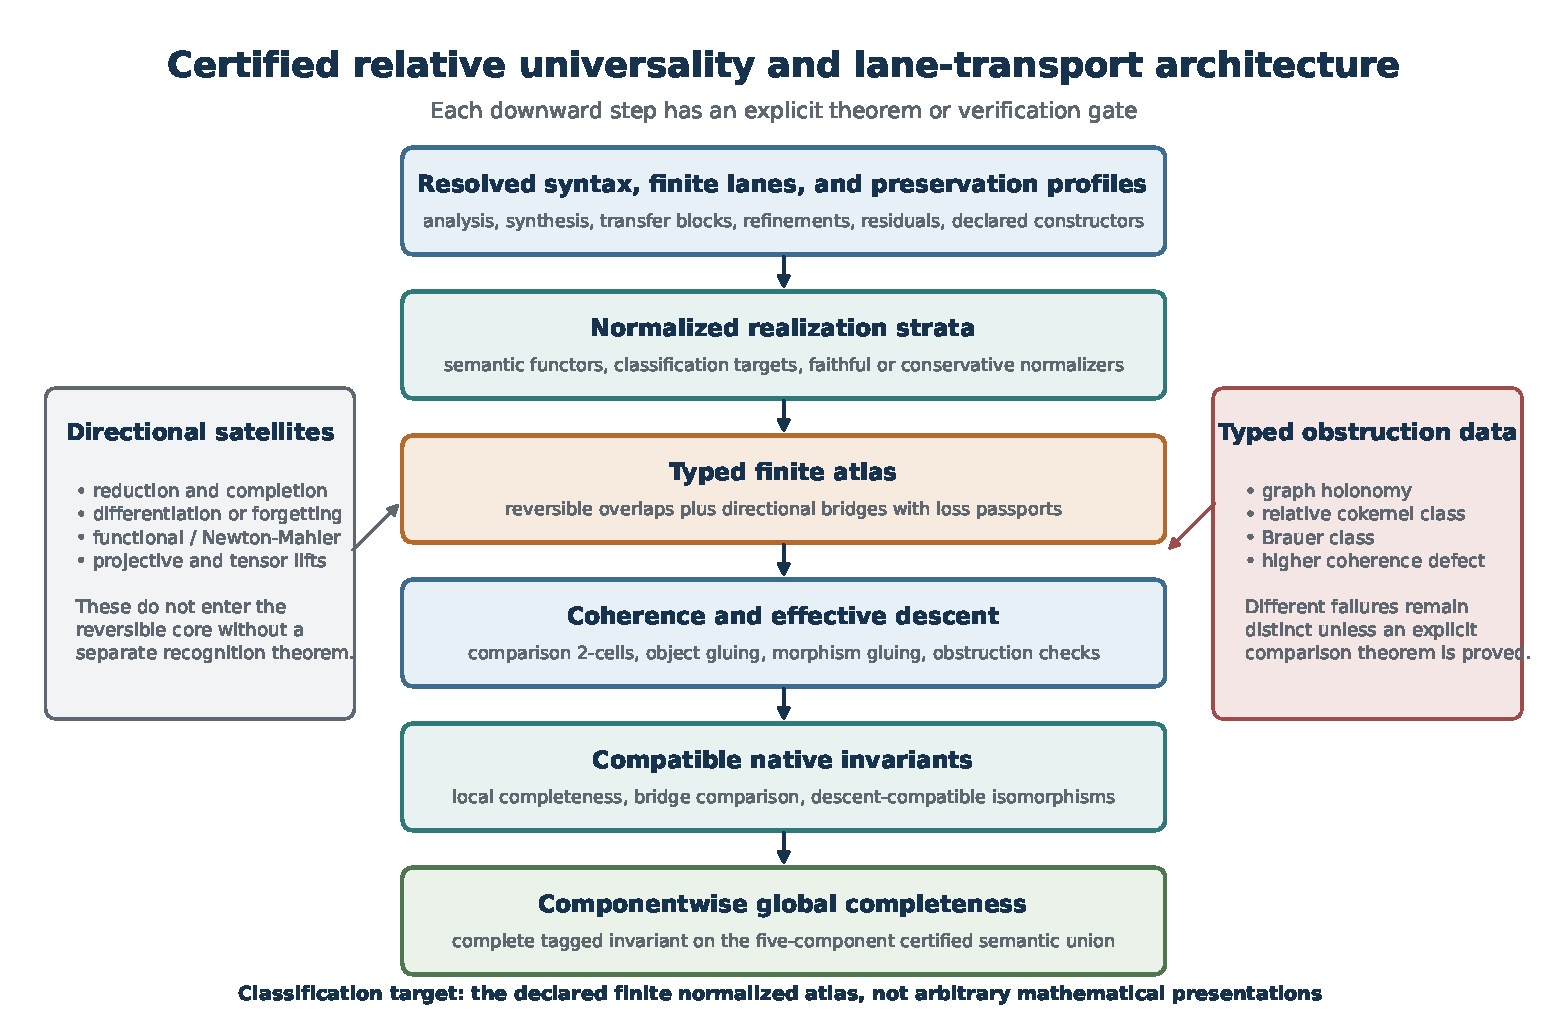
\includegraphics[width=.97\textwidth]{publication_proof_architecture.pdf}
\caption{Proof architecture of the journal-facing theorem.  The vertical spine contains the reversible construction and descent argument.  Directional satellites and obstruction data remain typed external inputs rather than silent equivalences.}
\label{fig:block14-publication-architecture}
\end{figure}


\part{Common foundations and finite assembly}
\section{Resolved theories, packet coordinates, and preservation profiles}
\label{sec:resolved-foundations}

This section expands the common formal core used by every later atlas construction.  The purpose is not to force every domain into one category.  It is to separate four layers that are often conflated:
\[
\boxed{
\text{typed syntax}
\longrightarrow
\text{resolved coordinates}
\longrightarrow
\text{profile-preserving realization}
\longrightarrow
\text{domain semantics}.}
\]
The first two layers are algebraic.  The third records which algebraic or universal constructions survive a realization.  The fourth supplies domain-specific hypotheses such as completeness, positivity, convergence, integrality, measurability, or analytic continuation.  A cross-domain statement is a theorem only when all four layers are present.

\subsection{Typed resolved signatures}
\label{subsec:typed-resolved-signatures}

\begin{definition}[Finite resolved signature]
\label{def:finite-resolved-signature}
Fix a commutative coefficient ring \(\kk\).  A finite resolved signature is a tuple
\[
\mathbb K_{\rm fin}
=
(Q,I,\mathsf P,\mathsf{Ref},\mathsf{Comp},\mathsf{Cert})
\]
with the following data.
\begin{enumerate}[label=\textup{(\roman*)}]
\item \(Q=(Q_0,Q_1,s,t)\) is a finite quiver.  Its vertices are sorts and its arrows are typed primitive operations.
\item \(I\triangleleft \kk Q\) is a finitely generated two-sided ideal generated by \(\kk\)-linear combinations of paths with common source and common target.
\item \(\mathsf P\) is a finite list of packet declarations.  A declaration on a sort \(X\) consists of endomorphism words \(p_{X,r,i}\) and the relations
\[
p_{X,r,i}p_{X,r,j}=\delta_{ij}p_{X,r,i},
\qquad
\sum_i p_{X,r,i}=1_X.
\]
\item \(\mathsf{Ref}\) is a finite list of refinement declarations.  For \(s\succeq r\), an address map
\[
\rho_{sr}:I_{X,s}\twoheadrightarrow I_{X,r}
\]
is accompanied by the equations
\[
p_{X,r,i}
=
\sum_{\rho_{sr}(j)=i}p_{X,s,j}.
\]
\item \(\mathsf{Comp}\) is a list of optional completion tags.  A tag names a doctrine to be added later, such as Banach completion, a \(C^*\)-involution, a multiplier completion, or a monoidal structure.  A tag is not itself an existence theorem.
\item \(\mathsf{Cert}\) is a list of named residual and certificate types.  Each certificate type specifies its source object, target object, and the equations or inequalities it is intended to record.
\end{enumerate}
\end{definition}

The finite signature is the presentation-level object.  It records legal words and declared equations.  It does not identify a preferred realization, a preferred coordinate basis, or a preferred semantic domain.

\begin{definition}[Realization of a finite resolved signature]
\label{def:resolved-realization}
Let \(\mathcal C\) be a \(\kk\)-linear category.  A realization of \(\mathbb K_{\rm fin}\) in \(\mathcal C\) assigns an object \(M_X\) to every vertex \(X\in Q_0\) and a morphism
\[
M_a:M_{s(a)}\longrightarrow M_{t(a)}
\]
to every arrow \(a\in Q_1\), such that all relations in \(I\), all packet equations, and all declared refinement equations hold.  Completion and certificate tags are interpreted only when the realization profile explicitly includes them.
\end{definition}

\begin{theorem}[Typed realization and module equivalence, imported]
\label{thm:typed-realization-module-equivalence}
Let
\[
\Lambda_{\mathbb K}:=\kk Q/I.
\]
In \(\kk\)-modules, the category of typed realizations of the linear grammar \((Q,I)\) is equivalent to the category of unital left \(\Lambda_{\mathbb K}\)-modules.  Under the equivalence, the vertex idempotent \(e_X\) acts as the projector onto the component of sort \(X\), and each arrow acts in its declared source-target block.
\end{theorem}

\begin{proof}
A typed realization defines the action of a path by composition and then extends \(\kk\)-linearly.  Every element of \(I\) acts by zero, so the action factors through \(\Lambda_{\mathbb K}\).  Conversely, for a unital module \(M\), the pairwise orthogonal vertex idempotents give
\[
M=\bigoplus_{X\in Q_0}e_XM,
\]
and an arrow \(a:X\to Y\) maps \(e_XM\) into \(e_YM\).  These constructions are inverse up to their canonical natural isomorphisms.  This is the typed-module theorem of Paper I \cite{P1}.
\end{proof}

\begin{remark}[Presentation is not classification]
\label{rem:presentation-not-classification}
The theorem fixes the semantics of one declared grammar.  It does not say that the grammar is unique, minimal, or recoverable from a finite list of observations.  Distinct quivers with relations can present equivalent module categories, and one realization can annihilate additional syntax through the kernel of its action.
\end{remark}

\begin{example}[Two-sort transfer grammar]
\label{ex:two-sort-transfer}
Take two sorts \(X,Y\), one arrow \(a:X\to Y\), and no nontrivial relation.  A realization is a single typed map
\[
M_X\xrightarrow{M_a}M_Y.
\]
After collapsing to \(M_X\oplus M_Y\), the vertex idempotents are coordinate packets and \(M_a\) is one off-diagonal transfer block.  The smallest typed grammar therefore already contains the distinction between object packets and transfer channels.
\end{example}

\subsection{Packet objects, analysis, and exact transfer coordinates}
\label{subsec:packet-coordinate-core}

\begin{definition}[Finite packet system]
\label{def:finite-packet-system-expanded}
Let \(X\) be an object of a preadditive category.  A finite packet system on \(X\) is a family
\[
\mathcal P=(p_i)_{i\in I}\subseteq\operatorname{End}(X)
\]
satisfying
\[
p_i^2=p_i,
\qquad
p_ip_j=0\quad(i\ne j),
\qquad
\sum_{i\in I}p_i=1_X.
\]
No self-adjointness or metric orthogonality is assumed unless stated separately.
\end{definition}

Assume now that \(\mathcal C\) is additive and idempotent complete.  Choose a splitting
\[
X_i\xrightarrow{\iota_i}X\xrightarrow{\pi_i}X_i,
\qquad
\iota_i\pi_i=p_i,
\qquad
\pi_i\iota_i=1_{X_i}.
\]
The packet equations imply
\[
\pi_i\iota_j=0\quad(i\ne j).
\]

\begin{definition}[Packet analysis and synthesis]
\label{def:packet-analysis-synthesis-expanded}
The packet analysis and synthesis maps are
\[
\Analysis_{\mathcal P}
:=
(\pi_i)_{i\in I}:
X\longrightarrow\bigoplus_{i\in I}X_i,
\]
\[
\Synthesis_{\mathcal P}
:=
(\iota_i)_{i\in I}:
\bigoplus_{i\in I}X_i\longrightarrow X.
\]
\end{definition}

\begin{theorem}[Exact packet-coordinate isomorphism, imported]
\label{thm:exact-packet-coordinate-expanded}
For every finite packet system in an additive idempotent-complete category,
\[
\boxed{
\Synthesis_{\mathcal P}\Analysis_{\mathcal P}=1_X,
\qquad
\Analysis_{\mathcal P}\Synthesis_{\mathcal P}
=1_{\oplus_iX_i}.}
\]
Consequently,
\[
X\cong\bigoplus_{i\in I}X_i.
\]
\end{theorem}

\begin{proof}
The first identity is
\[
\Synthesis_{\mathcal P}\Analysis_{\mathcal P}
=
\sum_i\iota_i\pi_i
=
\sum_i p_i
=
1_X.
\]
The \((i,j)\)-entry of the second composite is \(\pi_i\iota_j\), which equals \(1_{X_i}\) for \(i=j\) and zero otherwise.  This is the exact packet-coordinate theorem of Paper I \cite{P1}.
\end{proof}

\begin{corollary}[Packetwise equality]
\label{cor:packetwise-equality-expanded}
For parallel morphisms \(f,g:Z\to X\),
\[
f=g
\quad\Longleftrightarrow\quad
\pi_i f=\pi_i g\text{ for every }i.
\]
For parallel morphisms \(f,g:X\to Z\),
\[
f=g
\quad\Longleftrightarrow\quad
f\iota_i=g\iota_i\text{ for every }i.
\]
\end{corollary}

\begin{proof}
One direction is immediate.  In the other direction, insert the reconstruction identity on the appropriate side and sum the packetwise equalities.
\end{proof}

\begin{corollary}[Universal mapping property of packet coordinates]
\label{cor:packet-universal-expanded}
For every object \(Z\), restriction to the packet objects gives natural bijections
\[
\operatorname{Hom}(X,Z)
\cong
\prod_i\operatorname{Hom}(X_i,Z),
\qquad
\operatorname{Hom}(Z,X)
\cong
\prod_i\operatorname{Hom}(Z,X_i),
\]
where the products are finite.  Packetwise maps therefore assemble uniquely into a global map.
\end{corollary}

\begin{definition}[Mixed transfer blocks]
\label{def:mixed-transfer-blocks-expanded}
Let \(\mathcal P=(p_i)\) be a packet system on \(X\), let \(\mathcal Q=(q_a)\) be a packet system on \(Y\), and choose splittings \((\iota_i,\pi_i)\) and \((\jmath_a,\varpi_a)\).  For \(f:X\to Y\), define the packet-to-packet map
\[
f_{ai}:=\varpi_a f\iota_i:X_i\longrightarrow Y_a.
\]
Its ambient corner is
\[
q_afp_i=\jmath_a f_{ai}\pi_i.
\]
\end{definition}

\begin{theorem}[Exact transfer reconstruction and block composition, imported]
\label{thm:transfer-reconstruction-expanded}
Every morphism \(f:X\to Y\) has the exact expansion
\[
\boxed{
f
=
\sum_{a,i}q_afp_i
=
\sum_{a,i}\jmath_a f_{ai}\pi_i.}
\]
If \(g:Y\to Z\) is resolved by a packet system \(\mathcal R=(r_c)\), then
\[
\boxed{
(gf)_{ci}
=
\sum_a g_{ca}f_{ai}.}
\]
\end{theorem}

\begin{proof}
Insert the finite packet identities on both sides of \(f\):
\[
f
=
\left(\sum_aq_a\right)f\left(\sum_ip_i\right).
\]
For composition, insert \(1_Y=\sum_aq_a\) between \(g\) and \(f\).  This is the transfer-block reconstruction and multiplication law of Paper I \cite{P1}.
\end{proof}

\begin{corollary}[Path expansion]
\label{cor:packet-path-expansion}
For a composable string
\[
X_0\xrightarrow{f_1}X_1\xrightarrow{f_2}\cdots\xrightarrow{f_m}X_m
\]
with packet systems on every \(X_j\), each source-target block of \(f_m\cdots f_1\) is the sum over all compatible intermediate packet paths of the corresponding block products.
\end{corollary}

\begin{example}[Exact oblique packets]
\label{ex:oblique-packets}
Over any field, set
\[
p_1=
\begin{pmatrix}
1&1\\0&0
\end{pmatrix},
\qquad
p_2=
\begin{pmatrix}
0&-1\\0&1
\end{pmatrix}.
\]
Then \(p_1^2=p_1\), \(p_2^2=p_2\), \(p_1p_2=p_2p_1=0\), and \(p_1+p_2=I\).  The decomposition of \(\kk^2\) is exact, although the packets are not orthogonal for the standard inner product.  This separates the algebraic reconstruction theorem from later metric statements about energy or best approximation.
\end{example}

\subsection{Refinement, selected support, and named residuals}
\label{subsec:refinement-residual-calculus}

\begin{definition}[Finite refinement]
\label{def:finite-refinement-expanded}
A packet system \(\mathcal P^s=(p^s_j)_{j\in I_s}\) refines \(\mathcal P^r=(p^r_i)_{i\in I_r}\) when there is a surjection
\[
\rho_{sr}:I_s\twoheadrightarrow I_r
\]
such that
\[
p^r_i
=
\sum_{\rho_{sr}(j)=i}p^s_j.
\]
The map \(\rho_{sr}\) records the address of each fine packet inside its coarse ancestor.
\end{definition}

\begin{proposition}[Aggregation and transitivity]
\label{prop:refinement-aggregation-transitivity}
A finite aggregation of pairwise annihilating packets is again a packet system.  If \(t\succeq s\succeq r\), then refinement is transitive with address map
\[
\rho_{tr}=\rho_{sr}\circ\rho_{ts}.
\]
\end{proposition}

\begin{proof}
For an aggregated packet, idempotence follows because all cross terms vanish.  Distinct aggregates annihilate each other, and the total sum remains the identity.  Substituting the \(t\)-level expansion into the \(s\)-level expansion gives the composite address law.
\end{proof}

\begin{theorem}[Exact refinement law, imported]
\label{thm:exact-refinement-expanded}
Let \(p^r_i=\sum_{\rho_{sr}(j)=i}p^s_j\) and \(q^u_a=\sum_{\sigma_{vu}(b)=a}q^v_b\).  For every morphism \(f:X\to Y\),
\[
\boxed{
q^u_afp^r_i
=
\sum_{\sigma_{vu}(b)=a}
\sum_{\rho_{sr}(j)=i}
q^v_bfp^s_j.}
\]
Coarsening the fine block product of two composable maps gives the coarse block product.
\end{theorem}

\begin{proof}
Insert the two refinement identities on the left and right of \(f\).  For composition, expand both maps at the fine level, multiply, and sum over descendant intermediate packets.  The fine intermediate projectors sum to the coarse intermediate projector.  This is the exact refinement law of Resolution Theory \cite{RT}.
\end{proof}

\begin{definition}[Support compression and residual]
\label{def:support-compression-expanded}
For packet systems \(\mathcal P\) on \(X\) and \(\mathcal Q\) on \(Y\), let \(E\subseteq I_{\mathcal Q}\times I_{\mathcal P}\).  Define
\[
C_E(f):=\sum_{(a,i)\in E}q_afp_i,
\qquad
R_E(f):=f-C_E(f).
\]
The first term is the retained transfer support and the second is its named residual.
\end{definition}

\begin{proposition}[Boolean algebra of block selectors]
\label{prop:block-selector-algebra}
As endomorphisms of the \(\kk\)-module \(\operatorname{Hom}(X,Y)\), the selectors satisfy
\[
C_E^2=C_E,
\qquad
C_EC_F=C_{E\cap F},
\qquad
R_E=I-C_E.
\]
In particular,
\[
C_ER_E=R_EC_E=0,
\qquad
f=C_E(f)+R_E(f).
\]
\end{proposition}

\begin{proof}
Applying \(C_E\) to a block \(q_bfp_j\) retains it exactly when \((b,j)\in E\).  Pairwise annihilation removes every mismatched source or target index.  The formulas follow block by block.
\end{proof}

\begin{definition}[Relational support product]
\label{def:relational-support-product}
For \(E\subseteq I_Y\times I_X\) and \(F\subseteq I_Z\times I_Y\), define
\[
F\circ E
:=
\{(c,i):\text{there exists }a\in I_Y
\text{ with }(c,a)\in F\text{ and }(a,i)\in E\}.
\]
\end{definition}

\begin{proposition}[Support propagation under composition]
\label{prop:support-propagation}
If \(f=C_E(f)\) and \(g=C_F(g)\), then
\[
gf=C_{F\circ E}(gf).
\]
Thus exact zero patterns propagate by relational composition.
\end{proposition}

\begin{proof}
Every block of \(gf\) is a sum \(\sum_a g_{ca}f_{ai}\).  A nonzero summand can occur only along an intermediate address \(a\) belonging to the relational product.
\end{proof}

\begin{proposition}[Exact residual product identity]
\label{prop:exact-residual-product}
Let
\[
f_E=C_E(f),\quad r_f=R_E(f),
\qquad
g_F=C_F(g),\quad r_g=R_F(g).
\]
Then
\[
\boxed{
gf-g_Ff_E
=
r_gf_E+g_Fr_f+r_gr_f.}
\]
If the morphisms lie in a normed operator algebra with a submultiplicative norm, then
\[
\|gf-g_Ff_E\|
\le
\|r_g\|\,\|f_E\|
+\|g_F\|\,\|r_f\|
+\|r_g\|\,\|r_f\|.
\]
\end{proposition}

\begin{proof}
Substitute \(g=g_F+r_g\) and \(f=f_E+r_f\) and expand.  The norm estimate is immediate from the triangle inequality and submultiplicativity.
\end{proof}

The identity is a basic certificate-propagation law.  It explains exactly which residual terms enter after composing two compressed transfers.  No asymptotic claim is required.

\begin{theorem}[Hilbert--Schmidt optimality, imported]
\label{thm:hs-optimality-expanded}
Assume \(X,Y\) are Hilbert spaces, the packet idempotents are orthogonal projectors, and \(f:X\to Y\) is Hilbert--Schmidt.  Then \(C_E\) is the Hilbert--Schmidt orthogonal projection onto the selected block subspace and
\[
\|R_E(f)\|_{\mathrm{HS}}^2
=
\sum_{(a,i)\notin E}\|q_afp_i\|_{\mathrm{HS}}^2.
\]
Consequently, \(C_E(f)\) is the unique best Hilbert--Schmidt approximation to \(f\) among operators supported on \(E\).
\end{theorem}

\begin{boundary}[Algebraic exactness is not metric optimality]
\label{bnd:algebraic-vs-metric}
For arbitrary idempotent packets, reconstruction and residual decomposition remain exact.  Orthogonal energy identities and best-approximation statements require a Hilbert structure, orthogonal projectors, and the stated operator class.  Those hypotheses are part of the theorem rather than consequences of the packet notation.
\end{boundary}

\subsection{Preservation profiles and proof-support certificates}
\label{subsec:profile-calculus}

A realization can preserve one part of the resolved calculus and forget another.  The preservation profile is therefore a mathematical interface, not informal metadata.

\begin{definition}[Constructor universe]
\label{def:constructor-universe}
Fix a declared universe \(\mathfrak C\) of constructors and universal properties.  Typical entries are
\[
\begin{gathered}
0,\ 1,\ \text{finite sums},\ \text{composition},\ \text{scalar action},\ \text{biproducts},\\
\text{kernels},\ \text{cokernels},\ \text{quotients},\ \text{tensor products},\\
\text{packet idempotents},\ \text{transfer blocks},\ \text{refinements},\ \text{named residuals},\\
\text{finite limits},\ \text{finite colimits},\ \text{topological completions},\ \text{adjoints}.
\end{gathered}
\]
The list may be enlarged, but every new entry must specify the exact identity or universal property to be preserved.
\end{definition}

\begin{definition}[Verified preservation profile]
\label{def:verified-preservation-profile-expanded}
A verified preservation profile \(\Pi_F\) for a functor \(F:\mathcal C\to\mathcal D\) consists of a subset of \(\mathfrak C\) together with a proof or declared comparison isomorphism showing that \(F\) preserves each listed constructor.  We write \(c\in\Pi_F\) only after the corresponding preservation claim has been verified.
\end{definition}

\begin{definition}[Proof-support certificate]
\label{def:proof-support-certificate}
A proof-support certificate for a finite proof \(\mathcal P\) is a finite subset
\[
\operatorname{csupp}(\mathcal P)\subseteq\mathfrak C
\]
containing every constructor and universal property used in the proof.  The certificate need not be minimal.  It must be sufficient and auditable.
\end{definition}

\begin{proposition}[Common profile and composition]
\label{prop:common-profile-composition}
Let \(F:\mathcal C\to\mathcal D\) and \(G:\mathcal D\to\mathcal E\).  Every constructor preserved by both functors, with compatible chosen comparison data, is preserved by \(GF\).  For a finite diagram of realizations and bridges, the intersection
\[
\Pi_{\rm common}:=\bigcap_F\Pi_F
\]
is therefore a valid common profile for every proof transported through the whole diagram.
\end{proposition}

\begin{proof}
Preservation equations and comparison isomorphisms compose.  Universal properties remain universal after applying the second functor whenever both preservation witnesses are present.  Intersecting the verified lists retains only constructors supported at every stage.
\end{proof}

\begin{theorem}[Equational realization principle, imported]
\label{thm:equational-realization-expanded}
Let \(F:\mathcal C\to\mathcal D\) be additive between preadditive categories.  Every equality of morphism expressions built from declared generators by finite sums, additive inverses, identities, zero maps, and composition is preserved by \(F\).  Scalar multiplication is preserved when the categories are enriched over the same coefficient ring and \(F\) is linear.  If a proof additionally invokes a chosen biproduct, kernel, cokernel, quotient, tensor product, completion, or another universal construction, the proof transports only when that constructor belongs to \(\Pi_F\).
\end{theorem}

\begin{proof}
Functoriality preserves identities and composition.  Additivity preserves zero, sums, and additive inverses.  Linearity preserves the declared scalar action.  Structural induction on the morphism expression transports every equational step.  When a step is characterized by a universal property, the verified profile witness identifies the image construction with the corresponding target construction.  This is the equational realization principle of Paper I \cite{P1}.
\end{proof}

\begin{proposition}[Profile-safe theorem transport]
\label{prop:profile-safe-theorem-transport}
Let \(\mathcal P\) prove a statement \(T\) in the resolved syntax, and let \(F\) be a realization or bridge.  Suppose
\[
\operatorname{csupp}(\mathcal P)\subseteq\Pi_F.
\]
After every additional domain hypothesis used by \(T\) has been verified in the target, \(F(T)\) is a valid target theorem.  If the inclusion fails, the source proof does not by itself establish the target statement.
\end{proposition}

\begin{proof}
Apply \cref{thm:equational-realization-expanded} to every equational and universal-construction step in the proof certificate.  The remaining assumptions are precisely the domain-specific hypotheses, which are checked separately.
\end{proof}

\begin{definition}[Semantic realization certificate]
\label{def:semantic-realization-certificate}
A semantic realization certificate for transporting a theorem consists of four fields:
\begin{enumerate}[label=\textup{(C\arabic*)}]
\item an explicit functor or intertwining construction;
\item its verified preservation profile;
\item a proof-support certificate for the source theorem together with the inclusion into the profile;
\item verification of every target-specific hypothesis and a restatement of the conclusion in native target objects.
\end{enumerate}
\end{definition}

\begin{table}[htbp]
\centering
\caption{Typical preservation gates.  The right column names the extra obligation rather than asserting it automatically.}
\label{tab:preservation-gates}
\small
\begin{tabularx}{\textwidth}{@{}L{0.22\textwidth}L{0.25\textwidth}Y@{}}
\toprule
Proof step & Required profile entry & Additional target obligation\\
\midrule
Finite block identity & finite sums, composition, packet idempotents & verify that the declared packet equations hold\\
Kernel or cokernel argument & the corresponding universal property & check the target category has the selected construction\\
Quotient descent & quotient preservation & identify the target quotient and, topologically, its quotient topology\\
Infinite reconstruction & declared convergence/completion doctrine & specify norm, strong, weak, or unconditional convergence\\
Tensor reconstruction & tensor preservation and coherence & verify associativity, unit, and any symmetry or dagger structure used\\
Positivity or best approximation & adjoint, positivity, Hilbert structure & verify orthogonality and the relevant operator ideal\\
Arithmetic congruence & integral or local realization data & verify valuation, denominator, and reduction hypotheses\\
\bottomrule
\end{tabularx}
\end{table}

\begin{figure}[htbp]
\centering
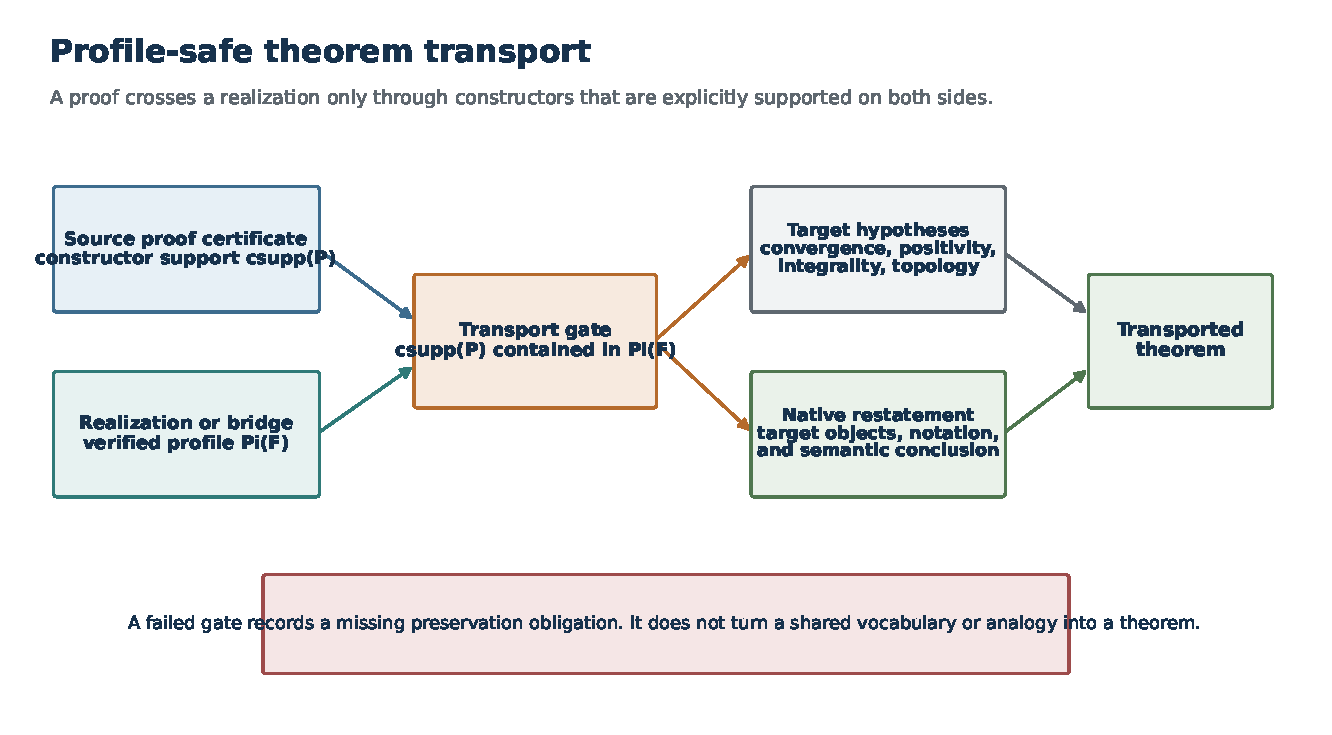
\includegraphics[width=0.98\textwidth]{profile_transport_gate.pdf}
\caption{The theorem-transport gate.  A shared vocabulary is not enough: the constructors used by the proof must lie inside the verified profile, and target-specific hypotheses must still be checked.}
\label{fig:profile-transport-gate}
\end{figure}

\begin{boundary}[Terminology is not semantic transport]
\label{bnd:terminology-not-transport}
Calling a frequency band, residue class, ramification sector, or latent channel a ``packet'' is only terminological reuse until the packet idempotents, reconstruction law, transfer blocks, and required preservation maps are supplied.  Failure of a profile gate is an explicit open obligation, not permission to infer the desired theorem by analogy.
\end{boundary}

\subsection{The finite additive-Karoubi resolved envelope}
\label{subsec:additive-karoubi-envelope-expanded}

The full profile-indexed envelope remains a multi-doctrine problem.  The finite linear, additive, and split-idempotent core can be constructed exactly.

\begin{definition}[Linear grammar category]
\label{def:linear-grammar-category}
For a finite linear resolved presentation \(\mathbb K_{\rm lin}=(Q,I,\mathsf P,\mathsf{Ref})\), let
\[
\mathcal A_{\mathbb K}:=\kk Q/I.
\]
This is the \(\kk\)-linear category whose objects are the vertices of \(Q\) and whose morphisms are \(\kk\)-linear combinations of typed paths modulo the declared relations.
\end{definition}

\begin{definition}[Finite additive hull]
\label{def:additive-hull-expanded}
The category \(\Add(\mathcal A_{\mathbb K})\) has finite tuples
\[
A=(A_1,\dots,A_m)
\]
as objects.  A morphism \(A\to B=(B_1,\dots,B_n)\) is an \(n\times m\) matrix with entries in \(\mathcal A_{\mathbb K}(A_j,B_i)\).  Composition is matrix multiplication using composition and addition in \(\mathcal A_{\mathbb K}\).
\end{definition}

\begin{definition}[Karoubi envelope]
\label{def:karoubi-envelope-expanded}
The Karoubi envelope \(\Kar(\Add(\mathcal A_{\mathbb K}))\) has pairs \((A,e)\), where \(e:A\to A\) is idempotent, as objects.  A morphism
\[
f:(A,e)\longrightarrow(B,d)
\]
is a morphism \(f:A\to B\) satisfying
\[
f=dfe.
\]
The identity on \((A,e)\) is \(e\).
\end{definition}

\begin{theorem}[Finite additive-Karoubi resolved envelope]
\label{thm:additive-karoubi-envelope}
The category
\[
\boxed{
\Syn_{\mathrm{ak}}(\mathbb K_{\rm lin})
:=
\Kar\!\bigl(\Add(\kk Q/I)\bigr)}
\]
is small, additive, idempotent complete, and \(\kk\)-linear.  For every additive idempotent-complete \(\kk\)-linear category \(\mathcal C\), restriction to the generating quiver induces an equivalence
\[
\Fun_{\kk}^{\oplus}
\bigl(\Syn_{\mathrm{ak}}(\mathbb K_{\rm lin}),\mathcal C\bigr)
\simeq
\Mod_{\mathrm{ak}}(\mathbb K_{\rm lin},\mathcal C),
\]
where the right side is the category of typed realizations satisfying all declared relations and carrying every declared packet idempotent to a split idempotent.
\end{theorem}

\begin{proof}
There are four universal stages.

\emph{Free typed stage.}  The free \(\kk\)-linear category on \(Q\) is universal for assigning objects to vertices and morphisms to arrows.

\emph{Relation stage.}  Quotienting by \(I\) imposes exactly the declared linear, packet, and refinement equations.  A functor out of \(\kk Q/I\) is therefore the same as a typed realization satisfying those equations.

\emph{Additive stage.}  Every \(\kk\)-linear functor from \(\kk Q/I\) into an additive category extends, uniquely up to canonical natural isomorphism, to an additive functor from the finite additive hull by sending a tuple to the corresponding biproduct and a matrix to its induced biproduct map.

\emph{Idempotent-splitting stage.}  Every additive functor into an idempotent-complete category extends, again uniquely up to canonical natural isomorphism, across the Karoubi envelope by sending \((A,e)\) to the chosen image of the split idempotent \(F(e)\).  Morphisms satisfying \(f=dfe\) descend to the corresponding split summands.

Composing these universal properties yields the displayed equivalence.  Smallness is preserved because only finite tuples and idempotents in hom sets of a small category are adjoined.
\end{proof}

\begin{proposition}[Fully faithful grammar embedding]
\label{prop:grammar-embedding}
The canonical composite
\[
\mathcal A_{\mathbb K}
\longrightarrow
\Add(\mathcal A_{\mathbb K})
\longrightarrow
\Kar(\Add(\mathcal A_{\mathbb K}))
\]
is fully faithful.  Thus the envelope adds finite biproducts and split summands without identifying two previously distinct grammar morphisms.
\end{proposition}

\begin{proof}
The first functor sends an object to the one-term tuple and preserves its hom set exactly.  The second sends \(A\) to \((A,1_A)\); its morphism condition is \(f=1_Bf1_A\), which imposes no additional relation.
\end{proof}

\begin{corollary}[Declared packets become literal objects]
\label{cor:packet-objects-literal}
Every declared idempotent \(p:X\to X\) defines an object \((X,p)\) of \(\Syn_{\mathrm{ak}}(\mathbb K_{\rm lin})\).  A complete packet family \((p_i)\) gives the canonical isomorphism
\[
(X,1_X)\cong\bigoplus_i(X,p_i).
\]
\end{corollary}

\begin{corollary}[Linear resolved strata as model categories]
\label{cor:linear-strata-model-categories}
Every additive split-idempotent realization stratum of \(\mathbb K_{\rm lin}\) is a category of profile-preserving functors out of \(\Syn_{\mathrm{ak}}(\mathbb K_{\rm lin})\).
\end{corollary}

\begin{example}[One operator and primary packets]
\label{ex:single-operator-envelope}
Take one sort, one endomorphism \(T\), and one relation \(\mu(T)=0\).  The linear grammar algebra is \(\kk[x]/(\mu)\).  When
\[
\mu=\mu_1\cdots\mu_r
\]
is a product of pairwise comaximal factors, the Chinese remainder idempotents define packet objects for the primary summands.  The envelope splits those idempotents formally.  Over a realization where the same factorization remains valid, the packet objects become the corresponding invariant primary sectors.
\end{example}

\begin{remark}[Universal does not mean presentation-minimal]
\label{rem:universal-not-minimal}
The envelope is universal for realizations of the declared presentation.  It does not provide a canonical smallest quiver, decide equivalence of arbitrary presentations, or identify a globally minimal packet system.  Those are recognition or minimization problems inside particular strata.
\end{remark}

\subsection{Profile-indexed extensions and the exact boundary of Foundation layer}
\label{subsec:profile-indexed-extension-boundary}

\begin{definition}[Profile-indexed resolved envelope]
\label{def:profile-indexed-envelope}
For a preservation profile \(\Pi\), a profile-indexed resolved envelope \(\Syn_\Pi(\mathbb K)\), when it exists, is a universal source satisfying
\[
\Mod_\Pi(\mathbb K,\mathcal C)
\simeq
\Fun_\Pi(\Syn_\Pi(\mathbb K),\mathcal C)
\]
for every target category \(\mathcal C\) carrying the structures named by \(\Pi\).  The equivalence must preserve the chosen comparison data, not only the underlying functors.
\end{definition}

\begin{table}[htbp]
\centering
\caption{Profile extensions beyond the proved additive-Karoubi core.}
\label{tab:profile-extensions}
\small
\begin{tabularx}{\textwidth}{@{}L{0.19\textwidth}L{0.28\textwidth}Y@{}}
\toprule
Doctrine & Additional data required & Boundary\\
\midrule
Nonlinear / operadic & colored finite-arity operations, symmetric actions, substitution, coherence & available locally in the nonlinear packet calculus, not freely present in every stratum\\
Banach / topological & topology, boundedness, convergence mode, completion and quotient-topology rules & algebraic packet sums do not choose a topology\\
\(C^*\) / \(W^*\) & involution, norm, positivity, closure, multiplier or weak completion & faithful corner realization does not automatically preserve an independent tensor product\\
Countable packets & strong, norm, weak, or unconditional convergence with boundedness controls & finite identities do not determine the infinite convergence doctrine\\
Monoidal / Tannakian & tensor product, unit, coherence, exact faithful fiber functor when reconstruction is claimed & ordinary faithful representation is weaker than monoidal reconstruction\\
Arithmetic / local & integral models, reductions, valuations, completeness, residue and lift data & denominator and reduction hypotheses remain domain-specific\\
\bottomrule
\end{tabularx}
\end{table}

\begin{figure}[htbp]
\centering
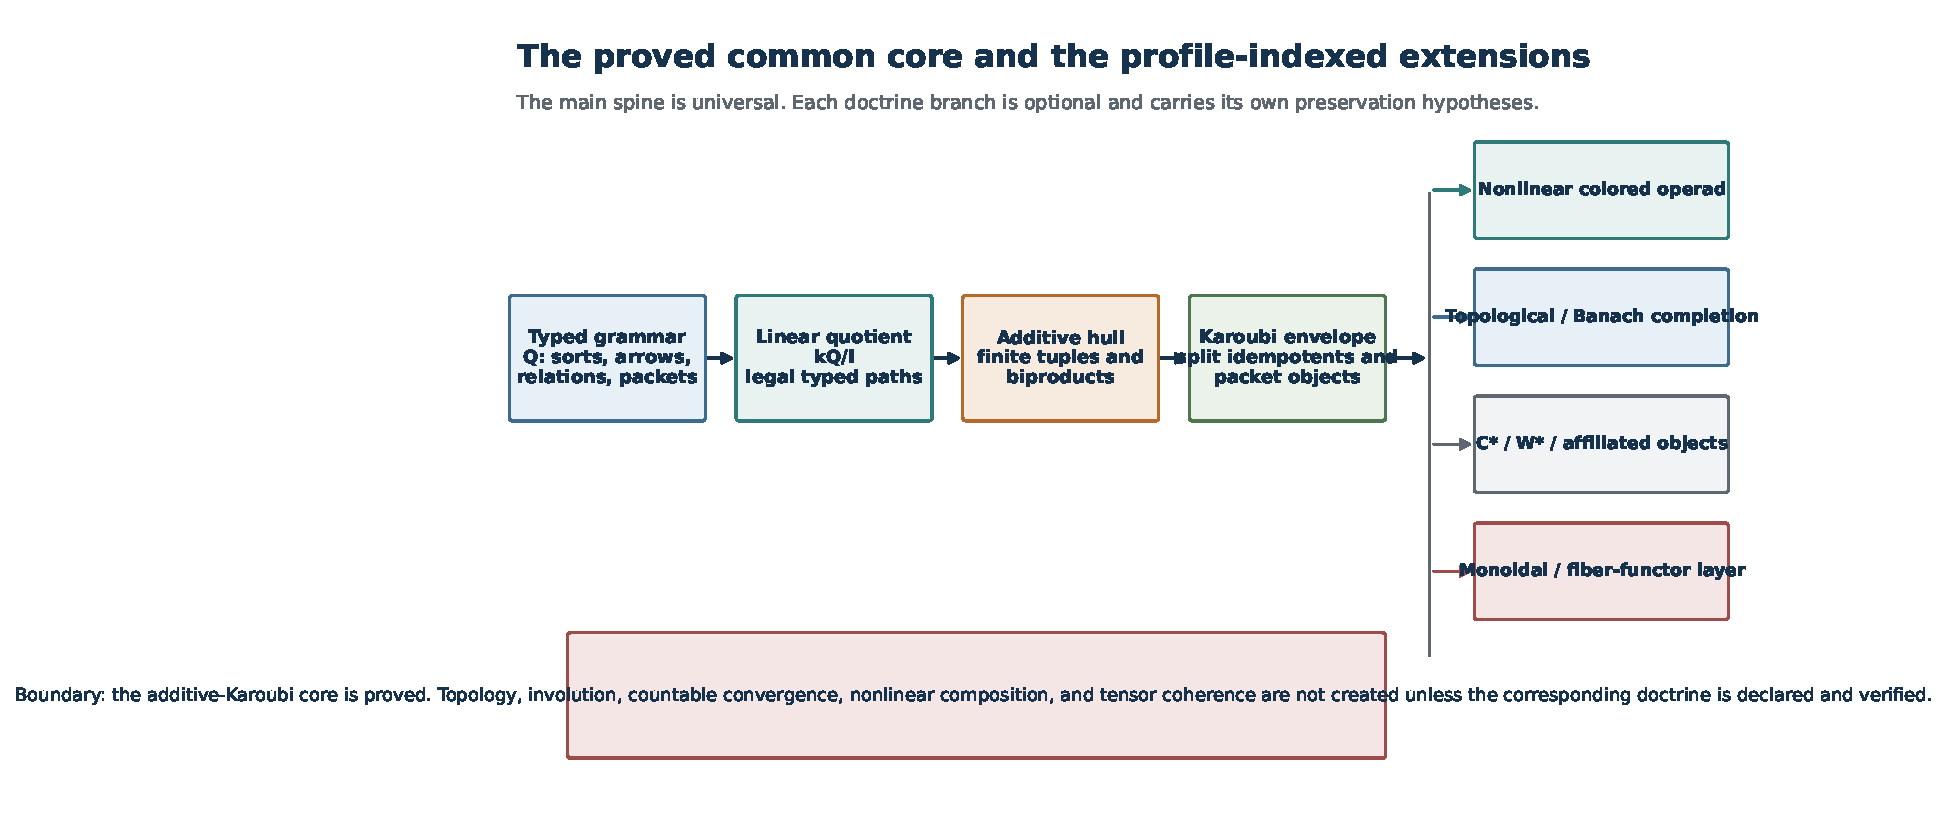
\includegraphics[width=0.99\textwidth]{foundation_envelope_stack.pdf}
\caption{The proved common envelope and the optional profile branches.  The branches should be added only for the strata that actually preserve them.}
\label{fig:foundation-envelope-stack}
\end{figure}

\begin{boundary}[No single overpowered envelope]
\label{bnd:no-overpowered-envelope}
The existence of \(\Syn_{\mathrm{ak}}\) does not prove the existence of one universal category simultaneously free, complete, \(C^*\), \(W^*\), nonlinear-operadic, monoidal, and arithmetically integral in a way preserved by every target.  The mathematically safer target is a family of profile-indexed envelopes or a doctrine-valued construction with explicit forgetful and comparison maps.
\end{boundary}

\begin{resultbox}
\textbf{Section result.}
The foundational language is now explicit at four levels: typed grammar semantics, exact finite packet and residual calculus, proof-support-controlled theorem transport, and the universal additive-Karoubi envelope.  The nonlinear, analytic, operator-algebraic, monoidal, and arithmetic envelopes remain separate profile obligations rather than hidden assumptions.
\end{resultbox}

\section{Strata, normalized charts, typed bridges, and obstruction objects}
\label{sec:strata-bridges-obstructions}

The common envelope developed in \cref{sec:resolved-foundations} is deliberately weaker than most concrete mathematical domains.  The next layer records how that envelope is realized, normalized, compared, and sometimes only partially remembered.  The central organizing rule is that a chart is not specified by a list of examples.  It is specified by a category of models, a preservation profile, a semantic functor, a normalized classification target, and explicit overlap data.

\subsection{Stratum passports and normalized model categories}
\label{subsec:stratum-passports}

\begin{definition}[Profiled stratum passport]
\label{def:profiled-stratum-passport}
A profiled Komorebi stratum is a record
\[
\mathbf S_\alpha
=
(\mathcal C_\alpha,\Pi_\alpha,\mathcal M_\alpha,
 \mathcal N_\alpha,\Sem_\alpha,\mathcal I_\alpha),
\]
with the following fields.
\begin{enumerate}[label=\textup{(\roman*)}]
\item \(\mathcal C_\alpha\) is the ambient semantic category in which the realized objects live.
\item \(\Pi_\alpha\) is the verified preservation profile of the realization.
\item \(\mathcal M_\alpha\) is a full replete category of admissible models of the declared resolved syntax.
\item \(\mathcal N_\alpha\subseteq\mathcal M_\alpha\) is a full replete normalized subcategory on which the intended inverse or classification theorem is stated.
\item
\[
\Sem_\alpha:\mathcal M_\alpha\longrightarrow\mathcal O_\alpha
\]
is the native semantics functor.
\item
\[
\mathcal I_\alpha:\Core(\mathcal N_\alpha)\longrightarrow\mathcal D_\alpha
\]
is a declared invariant functor, when one has been constructed.  Its codomain \(\mathcal D_\alpha\) and classification target are part of the record.
\end{enumerate}
The original four-field stratum
\((\mathcal C_\alpha,\Pi_\alpha,\mathcal M_\alpha,\Sem_\alpha)\)
remains the underlying realization datum.  The normalized and invariant fields are additional assembly data rather than automatic consequences.
\end{definition}

\begin{definition}[Normalization witness]
\label{def:normalization-witness}
A normalization witness on a full subcategory \(\mathcal U_\alpha\subseteq\mathcal M_\alpha\) consists of a functor
\[
N_\alpha:\mathcal U_\alpha\longrightarrow\mathcal N_\alpha
\]
and a natural isomorphism
\[
\nu_\alpha:\Sem_\alpha N_\alpha
\Longrightarrow
\Sem_\alpha|_{\mathcal U_\alpha}.
\]
It is \emph{classification-normalizing} when every object of \(\mathcal U_\alpha\) is semantically isomorphic to its image, and two normalized objects with isomorphic semantics are isomorphic in \(\mathcal N_\alpha\).  A normalization may be partial, domain-restricted, or defined only after auxiliary choices.  Those restrictions belong to the passport.
\end{definition}

\begin{definition}[Complete invariant on a declared target]
\label{def:complete-invariant-target}
An invariant \(\mathcal I_\alpha\) is complete on \(\mathcal N_\alpha\) when
\[
\mathcal I_\alpha(X)\cong\mathcal I_\alpha(Y)
\quad\Longleftrightarrow\quad
X\cong Y
\]
for all \(X,Y\in\mathcal N_\alpha\).  This statement classifies the objects of \(\mathcal N_\alpha\) up to the isomorphisms allowed there.  It does not classify arbitrary presentations outside that subcategory.
\end{definition}

\begin{proposition}[Semantic conservativity of a normalized chart]
\label{prop:normalized-semantic-conservativity}
If \(N_\alpha\) is classification-normalizing, then
\[
\Sem_\alpha|_{\mathcal N_\alpha}
\]
reflects isomorphisms.  Consequently, a complete invariant on \(\mathcal N_\alpha\) can be transported through a reversible overlap only after the overlap is shown to preserve the normalization and reflect the relevant isomorphisms.
\end{proposition}

\begin{proof}
Let \(X,Y\in\mathcal N_\alpha\) and suppose their semantic objects are isomorphic.  The second clause of \cref{def:normalization-witness} gives \(X\cong Y\).  The final statement follows because completeness is an assertion about isomorphism classes, not merely about equality of numerical outputs.
\end{proof}

\begin{figure}[htbp]
\centering
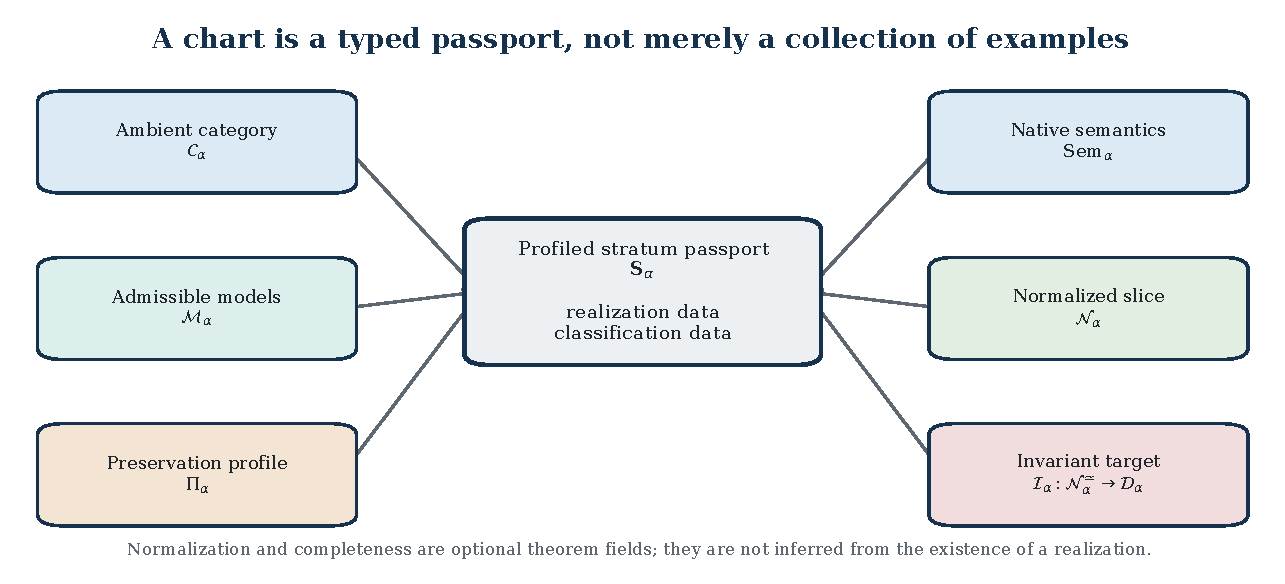
\includegraphics[width=0.98\textwidth]{stratum_passport.pdf}
\caption{A stratum passport separates the ambient category, admissible models, preservation profile, semantics, normalization, and invariant target.  Omitting any one of these fields makes cross-stratum classification claims ambiguous.}
\label{fig:stratum-passport}
\end{figure}

The present program uses the following principal strata.  The normalized fields are intentionally narrower than the ambient strata.  Several rows have exact slices but no canonical normalization for the whole broad class \cite{SEQ,GAL,FMH,NLO}.

\begin{landscape}
\scriptsize
\begin{longtable}{@{}L{0.095\linewidth}L{0.15\linewidth}L{0.135\linewidth}L{0.165\linewidth}L{0.19\linewidth}L{0.165\linewidth}@{}}
\caption{Current stratum passports at the level supported by the audited Library.  A dash means that no whole-stratum normalization theorem is asserted.}
\label{tab:stratum-passports}\\
\toprule
Stratum & Native objects & Native morphisms & Normalized or exact slice & Exact coordinate or invariant already available & Remaining boundary\\
\midrule
\endfirsthead
\toprule
Stratum & Native objects & Native morphisms & Normalized or exact slice & Exact coordinate or invariant already available & Remaining boundary\\
\midrule
\endhead
Finite linear and C-finite & finite recurrences, rational OGFs, finite linear states & intertwiners, recurrence changes, similarity & minimal recurrence, reduced OGF, reachable-observable state & Hankel rank, reduced denominator degree, minimal state dimension, torsion--Fourier subsequence profile & no classification of arbitrary nonminimal or mixed-grammar presentations\\
Holonomic & P-recursive sequences, D-finite functions, differential modules & coefficient/differential intertwiners & fixed operator convention and selected local data & effective P-recursive--D-finite translation; finite annihilator modules & minimal multisection operators, singularity orbits, monodromy aliasing, and cancellation signatures\\
Digital & DFAO, finite digit kernels, regular linear representations & state maps and radix-compatible intertwiners & minimal DFAO for fixed radix and reading direction & unique minimal DFAO up to state renaming; exact finite \(k\)-kernel compilation & no all-moduli packet profile or general linear-state minimality for \(k\)-regular systems\\
Algebraic & selected algebraic branches and packet polynomial systems & branch-preserving polynomial maps & a declared branch with a fixed defining system & exact packet polynomial realization and synthesis & minimal system dimension, branch-collision data, and effective packet-degree bounds\\
Nonlinear/tree & packet jets, colored operations, rooted-tree systems & operadic substitutions and smooth intertwiners & marked polynomial fixed points; positive simply generated tree families & packet Fa\`a di Bruno law, diagonal profile compression, SCC cyclic core, arity-gcd support and dominant-orbit signature & no global nonlinear normal form, mixed-direction universal compression, or coordinate-free minimal system dimension\\
Product and multiplicative & filtered Euler products, prime-power seed systems & exponent and local-factor maps & fixed Euler basis or declared multiplicative class & unique Euler exponents in the fixed basis; exact reconstruction from prime-power seeds & no canonical factorization across arbitrary product grammars and no general additive--multiplicative equivalence\\
Local, Mahler, and polyphase & Newton--Mahler coordinates, affine branches, functional masks, local states & affine restriction, refinement, Cartier and polyphase maps & fixed local chart and fixed modulus/radix conventions & unique Mahler coordinates, exact affine-polyphase transfer, exact Cartier automata for rational masks & no canonical global local normal form and no unrestricted bridge between functional and Newton--Mahler theories\\
Galois and Tannakian & semilinear packets, fixed-field charts, tensor representations & equivariant maps, induction/restriction, tensor morphisms & finite separable semisimple descent or neutral Tannakian fiber functor & Hilbert 90 descent, Brauer obstruction, subgroup/fixed-field classification, tensor reconstruction & modular and wild cases, and monoidal reconstruction without a verified fiber functor\\
\bottomrule
\end{longtable}
\end{landscape}

\begin{boundary}[Multiple valid placements]
\label{bnd:multiple-stratum-placements}
A semantic object may occur in several strata.  Catalan numbers, for example, may be algebraic, hypergeometric, P-recursive, and tree-generated.  The atlas records these as distinct presentations with certified bridges.  It does not force one placement to erase the others.
\end{boundary}

\subsection{Representation groupoids, gauge levels, and the directed transformation category}
\label{subsec:groupoid-directed}

For every stratum, the invertible part is the maximal subgroupoid
\[
\mathfrak{Rep}_\alpha(\bbK)
=
\Core(\mathcal M_\alpha).
\]
This core records changes of presentation that preserve all structure required by the overlap.  Quotients, truncations, completions, specializations, differential annihilator maps, and compression maps generally remain outside it.

\begin{definition}[Finite coordinate action groupoid]
\label{def:coordinate-action-groupoid}
Fix a dimension vector \(\mathbf d=(d_X)_{X\in\mathsf S}\).  Let
\[
G_{\mathbf d}=\prod_{X\in\mathsf S}GL_{d_X}(\kk)
\]
act on the finite-dimensional representation space \(\Rep_{\mathbf d}(\bbK)\) by base change.  The action groupoid
\[
[\Rep_{\mathbf d}(\bbK)/G_{\mathbf d}]
\]
has representations as objects and coordinate changes carrying one representation to another as morphisms.
\end{definition}

\begin{proposition}[Coordinate groupoid realizes isomorphism]
\label{prop:coordinate-groupoid-isomorphism}
Two objects of \(\Rep_{\mathbf d}(\bbK)\) are isomorphic as typed realizations exactly when they lie in the same \(G_{\mathbf d}\)-orbit.  The stabilizer of a point is its coordinate automorphism group.
\end{proposition}

\begin{proof}
A typed isomorphism is a family of invertible linear maps on the sort spaces intertwining every generating operation.  This is precisely an element of \(G_{\mathbf d}\) carrying one coordinate tuple to the other.  Elements fixing the tuple are exactly the typed automorphisms.
\end{proof}

Three symmetry levels must remain separate.

\begin{table}[htbp]
\centering
\caption{Three noninterchangeable symmetry notions.}
\label{tab:symmetry-levels}
\small
\begin{tabularx}{\textwidth}{@{}L{0.18\textwidth}L{0.26\textwidth}Y L{0.22\textwidth}@{}}
\toprule
Symmetry level & Acting object & What it changes or preserves & Extra hypothesis\\
\midrule
Gauge symmetry & coordinate-change group \(G_{\mathbf d}\) or a local gauge family & changes presentation coordinates while preserving the represented object & an explicitly typed action on the chart\\
Intrinsic symmetry & \(\Aut_{\mathcal M_\alpha}(M)\) & automorphisms of one resolved object inside the stratum & none beyond the native category\\
Reconstructed symmetry & \(\Aut^{\otimes}(\omega)\) & tensor automorphisms of a fiber functor and the corresponding affine group scheme & faithful exact tensor fiber functor\\
\bottomrule
\end{tabularx}
\end{table}

\begin{definition}[Typed directed transformation category]
\label{def:directed-transformation-category}
The directed transformation category \(\mathfrak{Dir}(\bbK)\) has pairs \((\alpha,M)\), with \(M\in\mathcal M_\alpha\), as objects.  A morphism
\[
(\alpha,M)\longrightarrow(\beta,N)
\]
is an admitted bridge instance equipped with a bridge passport as in \cref{def:bridge-passport}.  Composition is defined only when the codomain profile of the first bridge satisfies the domain requirements of the second.  The union of the representation groupoids embeds as the wide invertible subcategory.
\end{definition}

\begin{boundary}[Invertibility is evidence, not typography]
\label{bnd:invertibility-evidence}
Drawing a two-headed arrow does not make a bridge reversible.  A bridge enters the representation groupoid only after an inverse, quasi-inverse, or recognition theorem has been proved on a named overlap category.
\end{boundary}

\subsection{Bridge passports, bridge classes, and information-loss profiles}
\label{subsec:bridge-passports}

\begin{definition}[Bridge passport]
\label{def:bridge-passport}
A certified bridge from stratum \(\alpha\) to stratum \(\beta\) is a record
\[
\mathfrak b
=
(\mathcal U_\mathfrak b,\mathcal V_\mathfrak b,
 B_\mathfrak b,\tau_\mathfrak b,
 \Pi^{\mathrm{pres}}_\mathfrak b,
 \Pi^{\mathrm{refl}}_\mathfrak b,
 \Lambda_\mathfrak b,
 \nu_\mathfrak b,\chi_\mathfrak b),
\]
where:
\begin{enumerate}[label=\textup{(\roman*)}]
\item \(\mathcal U_\mathfrak b\subseteq\mathcal M_\alpha\) and \(\mathcal V_\mathfrak b\subseteq\mathcal M_\beta\) are the declared domain and codomain subcategories;
\item \(B_\mathfrak b:\mathcal U_\mathfrak b\to\mathcal V_\mathfrak b\) is the functor;
\item \(\tau_\mathfrak b\) is its bridge class;
\item \(\Pi^{\mathrm{pres}}_\mathfrak b\) records preserved constructors and universal properties;
\item \(\Pi^{\mathrm{refl}}_\mathfrak b\) records properties or isomorphisms reflected by the bridge;
\item \(\Lambda_\mathfrak b\) is the information-loss profile;
\item \(\nu_\mathfrak b\) is the semantic comparison map;
\item \(\chi_\mathfrak b\) records normalization, residual, and certificate compatibility.
\end{enumerate}
A passport may state that no inverse or no certificate transport is known.  Missing data remain missing rather than being inferred from analogy.
\end{definition}

The permitted bridge classes follow the work program in the controlling handoff.

\begin{table}[htbp]
\centering
\caption{Bridge classes used by the concrete atlas.}
\label{tab:bridge-classes}
\small
\begin{tabularx}{\textwidth}{@{}L{0.22\textwidth}L{0.20\textwidth}Y@{}}
\toprule
Class & Required evidence & Interpretation\\
\midrule
Equivalence & quasi-inverse and coherent unit/counit & reversible overlap of presentation groupoids\\
Fully faithful inclusion & bijections on hom-sets and full image description & no morphism loss inside the image, but possibly a smaller chart\\
Conservative forgetful functor & reflected isomorphisms & object equivalence remains detectable although structure may be forgotten\\
Information-losing directional functor & explicit semantic and loss statement & quotient, projection, annihilator, reduction, or compression\\
Constructor & proof that source data generate a target object & one-way realization, often with nonunique inverse data\\
Completion & topology and universal completion property & adds limits or closes a domain; reversibility requires a recognition theorem\\
Partially defined bridge & exact domain predicate & valid only on a named locus, branch, modulus, or regularity class\\
No certified bridge & none & no arrow is inserted into the trusted atlas\\
\bottomrule
\end{tabularx}
\end{table}

\begin{definition}[Information-loss profile]
\label{def:information-loss-profile}
For a functor \(B:\mathcal U\to\mathcal V\), its information-loss profile contains at least:
\begin{align*}
\operatorname{MorKer}_B(X,Y)
&=
\{(f,g)\in\Hom_{\mathcal U}(X,Y)^2:Bf=Bg\},\\
\operatorname{Coll}_B
&=
\{(X,Y)\in\operatorname{Ob}(\mathcal U)^2:BX\cong BY\},\\
\operatorname{EssIm}(B)
&\subseteq\mathcal V,
\end{align*}
together with the declared constructors, packet labels, residuals, certificates, branch data, topology, or arithmetic structure not preserved by \(B\).  The first component records morphism collapse, the second object collapse, and the third which target objects actually arise.
\end{definition}

\begin{definition}[Faithfulness, conservativity, and reversibility]
\label{def:lossless-bridge}
A bridge is:
\begin{enumerate}[label=\textup{(\roman*)}]
\item \emph{morphism-faithful} when every \(\operatorname{MorKer}_B(X,Y)\) is diagonal;
\item \emph{conservative} when \(Bf\) invertible implies that \(f\) is invertible;
\item \emph{classification-faithful} or \emph{essentially injective on objects} when \(BX\cong BY\) implies \(X\cong Y\) on the declared domain;
\item \emph{lossless on its image} when it is fully faithful;
\item \emph{reversible} when it is an equivalence onto the declared overlap.
\end{enumerate}
These conditions answer different questions and should not be conflated.
\end{definition}

\begin{proposition}[Composition law for bridge loss]
\label{prop:bridge-loss-composition}
Let
\[
\mathcal U\xrightarrow{B}\mathcal V\xrightarrow{C}\mathcal W
\]
be certified bridges.
\begin{enumerate}[label=\textup{(\roman*)}]
\item Every constructor or universal property preserved by both \(B\) and \(C\) is preserved by \(CB\).
\item
\[
\operatorname{MorKer}_B(X,Y)
\subseteq
\operatorname{MorKer}_{CB}(X,Y).
\]
\item
\[
\operatorname{Coll}_B
\subseteq
\operatorname{Coll}_{CB}.
\]
\item
\[
\operatorname{EssIm}(CB)
\subseteq
\operatorname{EssIm}(C).
\]
\item If both bridges are conservative, then their composite is conservative.  If both are classification-faithful, then their composite is classification-faithful.  If both are equivalences, then their composite is an equivalence.
\end{enumerate}
Thus information forgotten at an earlier stage cannot be recovered by merely composing more forgetful bridges, although a later bridge may attach auxiliary data through a separate constructor.
\end{proposition}

\begin{proof}
Functoriality proves the preservation claim.  If \(Bf=Bg\), then \(CBf=CBg\), proving the second inclusion.  If \(BX\cong BY\), applying \(C\) gives \(CBX\cong CBY\), proving the third.  Every object in the essential image of \(CB\) is visibly in the essential image of \(C\).  For conservativity, if \(CBf\) is invertible then \(Bf\) is invertible because \(C\) is conservative, and then \(f\) is invertible because \(B\) is conservative.  For classification-faithfulness, \(CBX\cong CBY\) implies \(BX\cong BY\) and then \(X\cong Y\).  Composition of equivalences is standard.
\end{proof}

\begin{figure}[htbp]
\centering
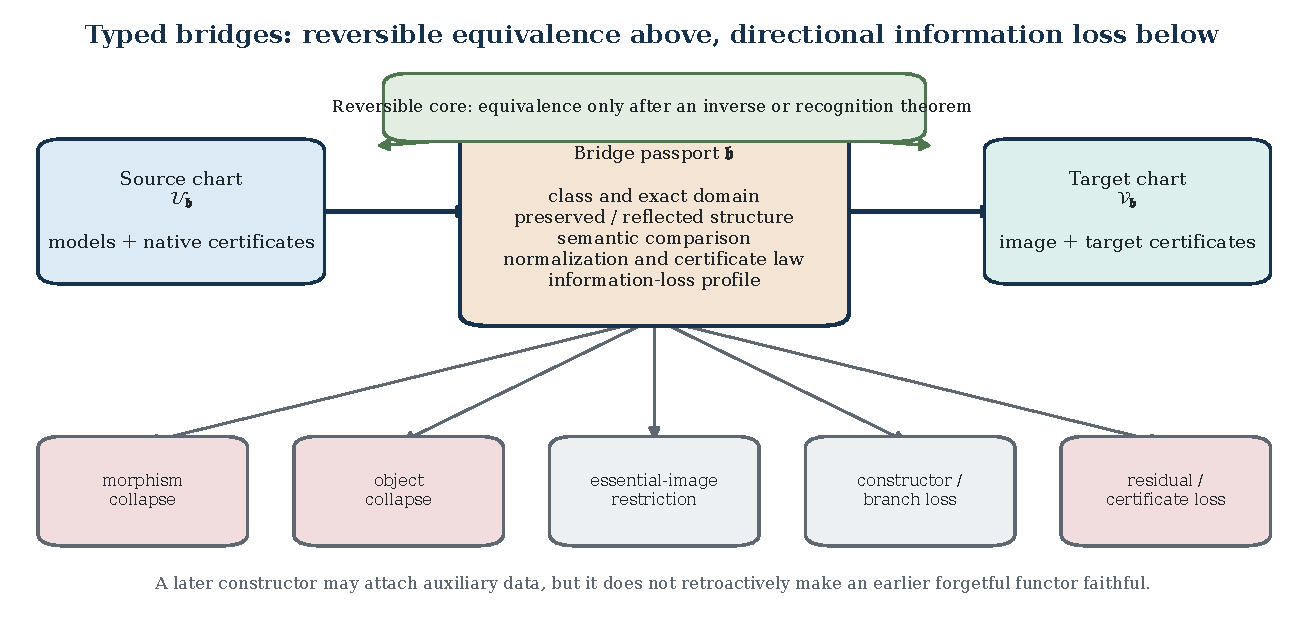
\includegraphics[width=0.98\textwidth]{bridge_passport_and_loss.pdf}
\caption{A bridge passport separates reversible equivalence from directional transformation and records the dimensions of information loss.  The reversible core is a theorem-level subcategory, not an informal interpretation of the whole bridge.}
\label{fig:bridge-passport-loss}
\end{figure}

Three typing cautions are especially important.

\begin{enumerate}
\item A selected algebraic branch can produce a D-finite annihilator, but the operator may forget the selected branch and its minimal polynomial.  The bridge is directional unless that data are retained.
\item A rational functional-Mahler mask over \(\mathbf F_p\) produces a Cartier representation and finite automaton under the stated hypotheses, but this does not identify it with a Newton--Mahler interpolation chart \cite{FMH,SEQ}.
\item A faithful Hilbert-space corner representation realizes packet projectors and transfers, but it does not automatically preserve a tensor product strongly enough for Tannakian reconstruction \cite{RT,GAL}.
\end{enumerate}

\subsection{Overlap categories and bridge-law certificates}
\label{subsec:overlap-categories}

\begin{definition}[Typed overlap]
\label{def:typed-overlap}
A reversible overlap between strata \(\alpha\) and \(\beta\) consists of full replete subcategories
\[
\mathcal M_{\alpha\beta}\subseteq\mathcal M_\alpha,
\qquad
\mathcal M_{\beta\alpha}\subseteq\mathcal M_\beta,
\]
an equivalence
\[
\Phi_{\alpha\beta}:\mathcal M_{\alpha\beta}
\overset{\sim}{\longrightarrow}
\mathcal M_{\beta\alpha},
\]
and a semantic natural isomorphism
\[
\sigma_{\alpha\beta}:
J_{\alpha\beta}\Sem_\alpha
\Longrightarrow
\Sem_\beta\Phi_{\alpha\beta}
\]
for an explicitly declared comparison functor \(J_{\alpha\beta}\) between the observable doctrines.  An overlap is \emph{normalized} when the equivalence restricts to the selected normalized subcategories.
\end{definition}

\begin{definition}[Bridge-law certificate]
\label{def:bridge-law-certificate}
A bridge-law certificate for \(B:\mathcal U\to\mathcal V\) records commuting or naturally commuting diagrams for each structure used downstream:
\begin{enumerate}[label=\textup{(\roman*)}]
\item native semantics;
\item packet analysis and synthesis;
\item refinement and coarsening maps;
\item selected-support compression and named residuals;
\item proof or computation certificates;
\item normalization and invariant comparison maps.
\end{enumerate}
For example, packet naturality requires comparison maps under which
\[
B(p_{Y,b}fp_{X,a})
\cong
p'_{B(Y),b}\,B(f)\,p'_{B(X),a},
\]
and refinement naturality requires the image of each coarse packet to equal the declared sum of its refined descendants.
\end{definition}

\begin{proposition}[Bridge-law transport]
\label{prop:bridge-law-transport}
Let \(\mathcal P\) be a proof whose constructor support lies in the preserved part of a bridge-law certificate.  Then the image proof is valid in the target chart.  If the proof concludes equality of normalized invariants, that equality descends across the bridge only when the normalization and invariant comparison maps are also included in the certificate.
\end{proposition}

\begin{proof}
The first statement is the equational realization principle of Paper I applied with the bridge-specific preservation profile.  The second statement follows because normalization and invariant functors are additional constructors in the proof diagram; they cannot be transported when their comparison cells are absent \cite{P1}.
\end{proof}

On triple overlaps, pairwise equivalences are not enough.  One needs comparison cells
\[
\eta_{\alpha\beta\gamma}:
\Phi_{\beta\gamma}\Phi_{\alpha\beta}
\Longrightarrow
\Phi_{\alpha\gamma}.
\]
For four charts, there are two composites from
\(
\Phi_{\gamma\delta}\Phi_{\beta\gamma}\Phi_{\alpha\beta}
\)
to \(\Phi_{\alpha\delta}\).  Their ratio is the higher coherence defect.

\begin{definition}[Quadruple-overlap coherence defect]
\label{def:quadruple-coherence-defect}
Write horizontal composition of natural transformations as \(\ast\).  Define
\[
\Omega_{\alpha\beta\gamma\delta}
=
\Bigl[
\eta_{\alpha\gamma\delta}
\circ
(\id\ast\eta_{\alpha\beta\gamma})
\Bigr]
\circ
\Bigl[
\eta_{\alpha\beta\delta}
\circ
(\eta_{\beta\gamma\delta}\ast\id)
\Bigr]^{-1}.
\]
It is a natural automorphism of \(\Phi_{\alpha\delta}\) on the quadruple overlap.  The atlas is coherent there exactly when
\[
\Omega_{\alpha\beta\gamma\delta}=\id.
\]
\end{definition}

\begin{proposition}[Two elementary coherence mechanisms]
\label{prop:elementary-coherence-mechanisms}
The coherence defect vanishes in either of the following situations.
\begin{enumerate}[label=\textup{(\roman*)}]
\item All overlap functors compose strictly and every comparison cell is the identity.
\item Between each pair of relevant normalized objects there is at most one admissible comparison isomorphism compatible with semantics.
\end{enumerate}
\end{proposition}

\begin{proof}
The first case is immediate.  In the second case, the two sides of the coherence equation are admissible comparison isomorphisms with the same source and target.  Uniqueness forces them to agree.  This is the mechanism used later in the normalized C-finite three-chart atlas.
\end{proof}

\begin{boundary}[Prestack versus stack]
\label{bnd:prestack-versus-stack}
Typed overlap functors and coherent comparison cells define atlas or prestack data.  The word \emph{stack} additionally requires effective descent: compatible local objects and morphisms must arise from global ones in the declared category.
\end{boundary}

\subsection{Reversible cores inside directional bridges}
\label{subsec:reversible-core-directional}

Directional maps can contain a canonical reversible overlap without being globally invertible.  Split packet analysis is the basic model.

\begin{theorem}[Split bridge rectification]
\label{thm:split-bridge-rectification}
Let \(\mathcal A\) be an additive idempotent-complete category and suppose
\[
X\xrightarrow{A}Y\xrightarrow{L}X
\]
satisfies \(LA=\id_X\).  Put \(E=AL\).  Then:
\begin{enumerate}[label=\textup{(\roman*)}]
\item \(E^2=E\);
\item \(Y\cong\im E\oplus\im(1-E)\);
\item \(A:X\to\im E\) is an isomorphism with inverse induced by \(L\);
\item \(L(1-E)=0\), so \(\im(1-E)\) is a named residual invisible to the decoder;
\item the directional two-chart system becomes reversible after restricting the packet chart to the consistent core \(\im E\).
\end{enumerate}
In a module or vector-space realization, \(\im(1-E)=\ker L\).
\end{theorem}

\begin{proof}
The identity \(E^2=A(LA)L=AL=E\) proves the first statement.  Idempotent completeness splits \(E\), producing the direct sum.  The image of \(A\) lies in \(\im E\), and \(L A=\id_X\) while \(A L=E\) acts as the identity on \(\im E\), so the restricted maps are inverse.  Finally,
\[
L(1-E)=L-LAL=L-L=0.
\]
For modules, every \(y\in\ker L\) satisfies \((1-E)y=y\), while every vector in \(\im(1-E)\) is killed by \(L\).
\end{proof}

\begin{corollary}[Exact meaning of a decoded packet core]
\label{cor:decoded-packet-core}
A left inverse proves exact recovery on the consistent packet core.  It does not prove that every ambient packet vector is consistent, that the residual is small, or that the packet representation is compressed.  Those are separate geometric, analytic, or coding claims.
\end{corollary}

The integral Mahler packet theorem is a concrete instance: the analysis matrix has an integer left inverse, the consistency projector is \(AL\), and the residual is the complementary packet component.  The same decoder survives every base change, while rank loss of individual residue channels remains visible after reduction \cite{CT4}.

\subsection{Finite holonomy and the maximal path-flat core}
\label{subsec:maximal-flat-core}

Finite graph transport gives the sharpest reversible gluing model in the Library.  Let \(\Gamma=(V,E)\) be a finite connected graph.  Attach a finite-dimensional \(\kk\)-vector space \(F_v\) to each vertex and an isomorphism \(T_e:F_u\to F_v\) to each oriented edge \(e:u\to v\), with \(T_{\bar e}=T_e^{-1}\).  Choose a root \(o\) and spanning tree \(S\).  If \(G_v:F_o\to F_v\) is tree transport, then every non-tree edge \(e:u\to v\) has fundamental holonomy
\[
H_e=G_v^{-1}T_eG_u\in GL(F_o).
\]
Define
\[
C_o
=
\bigcap_{e\notin S}\ker(H_e-I)
=
\Fix\langle H_e:e\notin S\rangle,
\qquad
C_v=G_vC_o.
\]

\begin{theorem}[Maximal flat core and global sections]
\label{thm:maximal-flat-core}
Under the preceding hypotheses \cite{P3,CT4}:
\begin{enumerate}[label=\textup{(\roman*)}]
\item evaluation at the root identifies the space of global parallel sections with \(C_o\);
\item \((C_v)_v\) is path-flat, meaning that all path transports with the same endpoints agree on the core;
\item it is the unique greatest path-flat subfamily;
\item it is independent of the chosen spanning tree and equals the common fixed space of all closed-path holonomies;
\item for
\[
\Delta_S:F_o\longrightarrow\bigoplus_{e\notin S}F_o,
\qquad
\Delta_Sx=((H_e-I)x)_{e\notin S},
\]
one has
\[
C_o=\ker\Delta_S,
\qquad
\dim C_o=\dim F_o-\rank\Delta_S;
\]
\item the full fibers glue to one global frame exactly when every fundamental holonomy is the identity;
\item a gauge change conjugates the holonomies and transports the core, so \(\dim C_o\) is gauge-invariant.
\end{enumerate}
\end{theorem}

\begin{proof}
For \(x\in C_o\), set \(x_v=G_vx\).  Tree edges satisfy the parallel relation by construction, and a non-tree edge satisfies it because \(H_ex=x\).  Conversely, any global section is determined along the tree by its root value; every remaining edge forces that value to be fixed by the corresponding \(H_e\).  This proves the section classification.  Closed paths are words in fundamental cycles, which gives path-flatness and tree independence.  Any path-flat family must be fixed by every fundamental cycle and is therefore contained in \((C_v)_v\).  The rank formula is rank--nullity.  Full flatness and gauge covariance follow from spanning-tree normalization and conjugation of loop products.
\end{proof}

\begin{corollary}[Global section versus global frame]
\label{cor:global-section-versus-frame}
Nonidentity holonomy can leave a nonzero maximal core.  Therefore the existence of some global compatible vectors is weaker than the existence of one global frame on the full fibers.  The former is measured by \(\dim C_o\); the latter requires \(C_o=F_o\).
\end{corollary}

\begin{figure}[htbp]
\centering
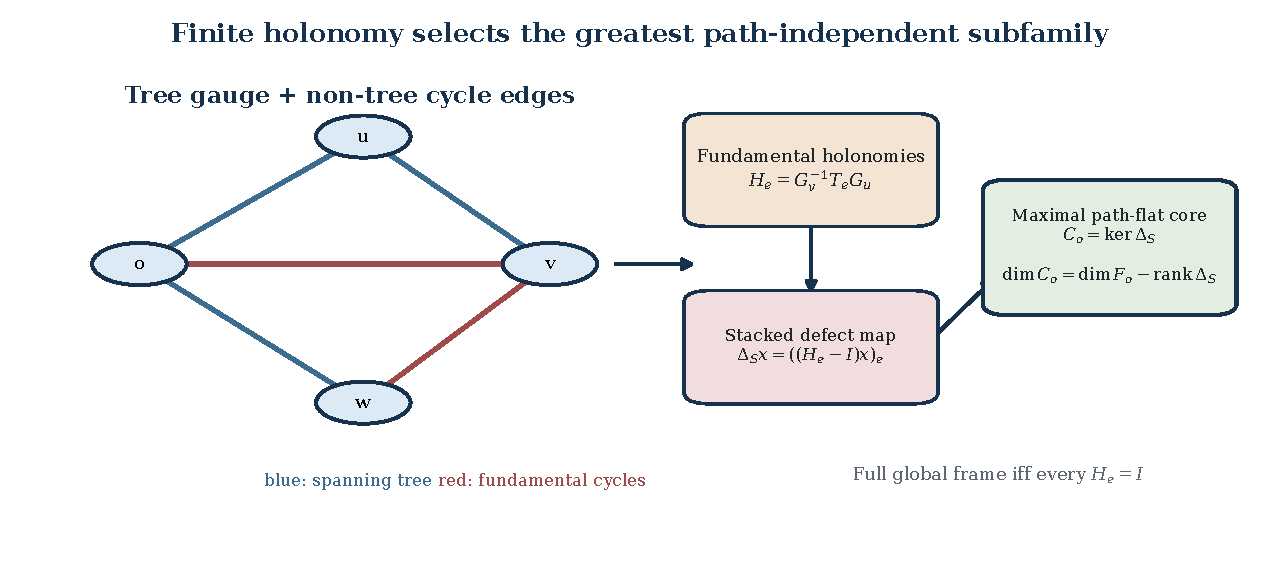
\includegraphics[width=0.96\textwidth]{flat_core_holonomy.pdf}
\caption{A spanning tree removes local gauge redundancy.  Each remaining edge contributes a fundamental holonomy.  Their common fixed space is the maximal path-flat core; the stacked defect map \(\Delta_S\) measures the lost dimension.}
\label{fig:flat-core-holonomy}
\end{figure}

\subsection{Relative cokernel obstructions and loss under coarsening}
\label{subsec:relative-cokernel-obstruction}

Holonomy addresses compatibility of invertible transports.  Correction problems have a different canonical object.

\begin{definition}[Linear correction datum]
\label{def:block02-linear-correction}
A linear correction datum is a map
\[
D:U\longrightarrow V
\]
and a defect \(r\in V\).  A correction is \(u\in U\) satisfying \(Du=-r\).  The relative obstruction class is
\[
\Ob_D(r)=[r]\in\coker D=V/\im D.
\]
\end{definition}

\begin{theorem}[Cokernel criterion, universality, and naturality]
\label{thm:block02-cokernel-naturality}
For a correction datum \((D,r)\) \cite{P3}:
\begin{enumerate}[label=\textup{(\roman*)}]
\item a correction exists if and only if \(\Ob_D(r)=0\);
\item every linear obstruction test \(\varphi:V\to W\) satisfying \(\varphi D=0\) factors uniquely through \(V\to\coker D\);
\item for every commuting square
\[
\begin{array}{ccc}
U & \xrightarrow{D} & V\\
\downarrow a & & \downarrow b\\
U' & \xrightarrow{D'} & V',
\end{array}
\qquad bD=D'a,
\]
there is a unique induced map
\[
\overline b:\coker D\longrightarrow\coker D'
\]
with
\[
\overline b\,\Ob_D(r)=\Ob_{D'}(br).
\]
\end{enumerate}
\end{theorem}

\begin{proof}
The class vanishes exactly when \(r\in\im D\), which is equivalent to solvability of \(Du=-r\).  A map annihilating \(\im D\) factors uniquely through the quotient.  In the square, the quotient map for \(D'\), composed with \(b\), vanishes on \(\im D\), so the same universal property produces \(\overline b\).
\end{proof}

\begin{proposition}[Packet coordinates on the obstruction quotient]
\label{prop:block02-obstruction-packets}
Suppose \((Q_a)\) is a complete finite family of pairwise annihilating idempotents on \(V\) and
\[
Q_a(\im D)\subseteq\im D
\]
for every \(a\).  Then the \(Q_a\) descend to quotient idempotents \(\overline Q_a\) on \(\coker D\),
\[
\coker D
\cong
\bigoplus_a\overline Q_a(\coker D),
\qquad
\overline Q_a\Ob_D(r)=[Q_ar].
\]
If \(U\) and \(V\) already split into matching packet summands and \(D\) is block diagonal, this becomes
\[
\coker D\cong\bigoplus_a\coker D_a.
\]
Off-diagonal correction blocks can couple packet defects, so the block-diagonal hypothesis cannot be omitted.
\end{proposition}

\begin{proof}
The invariance of \(\im D\) makes \([v]\mapsto[Q_av]\) well defined.  Idempotence, annihilation, and reconstruction descend to the quotient.  In the block-diagonal case the image of \(D\) is the direct sum of the images of the restrictions.
\end{proof}

A coarse representation can erase a nonzero fine obstruction.  The strengthened Paper III gives the exact bookkeeping device.

\begin{theorem}[Relative obstruction exact sequence]
\label{thm:block02-relative-obstruction-sequence}
Suppose the diagram
\[
\begin{array}{ccccccccc}
0&\to&U_0&\to&U_f&\to&U_c&\to&0\\
 &&\downarrow D_0&&\downarrow D_f&&\downarrow D_c\\
0&\to&V_0&\to&V_f&\to&V_c&\to&0
\end{array}
\]
commutes and has exact rows.  Then there is a natural exact sequence
\[
\begin{aligned}
0&\longrightarrow\ker D_0
\longrightarrow\ker D_f
\longrightarrow\ker D_c
\xrightarrow{\delta}\coker D_0\\
&\longrightarrow\coker D_f
\longrightarrow\coker D_c
\longrightarrow0.
\end{aligned}
\]
If a fine obstruction maps to zero in \(\coker D_c\), then it comes from \(\coker D_0\), the obstruction sector removed by coarsening.  Coarse vanishing therefore does not imply fine vanishing.
\end{theorem}

\begin{proof}
This is the direct kernel--cokernel sequence proved in the strengthened Paper III.  The connecting map lifts an element of \(\ker D_c\) to \(U_f\), applies \(D_f\), identifies the result in \(V_0\), and takes its class modulo \(\im D_0\).  Exactness verifies independence of the lift and identifies each successive kernel with the preceding image \cite{P3,MIG}.
\end{proof}

\begin{example}[A fine obstruction erased by summation]
\label{ex:fine-obstruction-erased}
Take all correction spaces to be zero,
\[
V_f=\kk^2,
\qquad
V_c=\kk,
\qquad
p(x,y)=x+y.
\]
The fine defect \((1,-1)\) is nonzero in \(\coker D_f=V_f\), but its coarse image is zero.  It lies entirely in
\[
V_0=\ker p=\Span\{(1,-1)\}.
\]
This is cancellation by coarsening, not correction of the fine defect.
\end{example}

\begin{definition}[Mapping cone]
\label{def:block02-mapping-cone}
For a cochain map \(D:C^\bullet\to E^\bullet\), define
\[
\Cone(D)^n=E^n\oplus C^{n+1},
\qquad
 d_{\Cone}(e,c)=(d_Ee+Dc,-d_Cc).
\]
\end{definition}

\begin{proposition}[Cohomological correction criterion]
\label{prop:block02-cone-obstruction}
For a cocycle \(e\in E^n\), the class of \((e,0)\) in \(H^n(\Cone(D))\) vanishes exactly when \([e]\) lies in the image of \(H^n(D)\).  When the complexes are concentrated in degree zero,
\[
H^0(\Cone(D))\cong\coker D.
\]
\end{proposition}

\begin{proof}
The class of \((e,0)\) is a boundary exactly when there are \(e'\in E^{n-1}\) and \(c\in C^n\) with
\[
e=d_Ee'+Dc,
\qquad
d_Cc=0.
\]
This is equivalent to \([e]=H^n(D)[c]\).  Concentration in degree zero reduces the cone quotient to \(E^0/\im D\).
\end{proof}

\begin{boundary}[The correction map is problem data]
\label{bnd:correction-map-problem-data}
The cokernel is canonical relative to \(D\).  The theory does not yet supply one choice-free rule that constructs the correct \(D\) for every mathematical problem and every stratum.  Calling \([r]\in\coker D\) canonical must not hide this dependence.
\end{boundary}

\subsection{Semilinear effectivity, projective descent, and the Brauer class}
\label{subsec:brauer-descent}

Galois descent gives a second exact local-to-global model.  Its linear and projective cases separate effectivity from obstruction sharply.

\begin{theorem}[Effective vector descent by Hilbert 90]
\label{thm:block02-hilbert90}
Let \(L/K\) be finite Galois with group \(G\).  Suppose
\[
a_{\sigma\tau}=a_\sigma\,\sigma(a_\tau),
\qquad
a_\sigma\in GL_n(L),
\]
defines a semilinear packet cocycle.  Then there is \(B\in GL_n(L)\) such that
\[
a_\sigma=B^{-1}\sigma(B).
\]
The twisted fixed packet
\[
W=(L^n)^{G,\star}
\]
is an \(n\)-dimensional \(K\)-vector space and
\[
W\otimes_KL\xrightarrow{\sim}L^n.
\]
Thus every finite linear semilinear atlas of this form is effective \cite{GAL}.
\end{theorem}

\begin{theorem}[Brauer obstruction to projective packet descent]
\label{thm:block02-brauer}
Projective semilinear descent data define a class
\[
\alpha\in H^1(G,PGL_n(L)).
\]
The connecting map for
\[
1\longrightarrow L^\times
\longrightarrow GL_n(L)
\longrightarrow PGL_n(L)
\longrightarrow1
\]
produces
\[
\delta(\alpha)
\in
H^2(G,L^\times)
=
\Br(L/K).
\]
The projective atlas lifts to linear semilinear descent data exactly when \(\delta(\alpha)=0\).  When the class is nonzero, the descended object is naturally a module over a central simple \(K\)-algebra split by \(L\), rather than an ordinary \(K\)-vector space \cite{GAL}.
\end{theorem}

\begin{proof}
This is the nonabelian cohomology exact sequence together with nonabelian Hilbert 90.  Vanishing of the connecting class gives a \(GL_n(L)\)-valued cocycle; \cref{thm:block02-hilbert90} then trivializes it and constructs the descended vector space.  A nonzero class is the classical relative Brauer obstruction.
\end{proof}

\begin{corollary}[Projective compatibility is not linear effectivity]
\label{cor:projective-not-linear-effectivity}
A projective atlas may satisfy every visible overlap equation in \(PGL_n\) and still have no global vector-space realization.  Projective cocycle coherence and vanishing Brauer class are distinct conditions.
\end{corollary}

The tensor reconstruction problem lies beyond ordinary corner realization.

\begin{theorem}[Tannakian boundary]
\label{thm:block02-tannakian-boundary}
Let \(\mathcal T\) be a neutral Tannakian category over \(k\) and
\[
\omega:\mathcal T\longrightarrow\operatorname{Vect}_k
\]
a faithful exact tensor fiber functor.  Then
\[
\mathcal G=\Aut^{\otimes}(\omega)
\]
is an affine group scheme and
\[
\mathcal T\simeq\operatorname{Rep}_k(\mathcal G)
\]
as tensor categories.  A faithful projector-corner representation without verified exact strong monoidal structure does not cross this boundary \cite{GAL,RT}.
\end{theorem}

\subsection{Higher coherence defects and typed obstruction comparison}
\label{subsec:obstruction-comparison}

The four obstruction families now admit a precise comparison.  Each starts from different data and answers a different vanishing question.

\begin{landscape}
\small
\begin{longtable}{@{}L{0.14\linewidth}L{0.20\linewidth}L{0.20\linewidth}L{0.20\linewidth}L{0.18\linewidth}@{}}
\caption{Typed obstruction comparison.}
\label{tab:obstruction-comparison}\\
\toprule
Failure mode & Required datum & Obstruction object & Vanishing consequence & Nonzero meaning\\
\midrule
\endfirsthead
\toprule
Failure mode & Required datum & Obstruction object & Vanishing consequence & Nonzero meaning\\
\midrule
\endhead
Finite transport holonomy & connected graph, invertible edge transports, chosen structure group & fundamental cycle holonomies or the conjugacy class of \(\pi_1(\Gamma)\to G\) & one global frame on the full fibers; on a fixed subspace, path-independent transport & path dependence; possibly a smaller nonzero fixed core\\
Relative correction failure & correction map \(D:U\to V\) and defect \(r\) & \([r]\in\coker D\), or a mapping-cone cohomology class & an allowed correction exists & the defect is outside the declared correction image\\
Projective Galois descent & projective semilinear cocycle over \(L/K\) & \(\delta(\alpha)\in H^2(G,L^\times)=\Br(L/K)\) & lift to linear descent, then effective vector descent by Hilbert 90 & descent to a twisted central-simple-algebra object rather than an ordinary vector space\\
Higher atlas coherence & pairwise equivalences and comparison \(2\)-cells & \(\Omega_{\alpha\beta\gamma\delta}\), a natural automorphism on a quadruple overlap & pseudofunctor coherence of the atlas & pairwise bridges use incompatible conventions or incomplete comparison data\\
\bottomrule
\end{longtable}
\end{landscape}

\begin{proposition}[Typed comparison principle for obstruction objects]
\label{prop:typed-obstruction-comparison}
An obstruction object transports from one problem to another only after a compatibility morphism for the underlying data has been supplied:
\begin{enumerate}[label=\textup{(\roman*)}]
\item commuting squares of correction maps induce maps on cokernels;
\item group homomorphisms or intertwiners compatible with edge transports induce maps on holonomy data and fixed cores;
\item morphisms of the relevant central extensions induce maps on cohomological descent obstructions;
\item modifications of atlas pseudofunctors transport higher coherence defects.
\end{enumerate}
Absent such typed data, there is no canonical reduction of one obstruction family to another.
\end{proposition}

\begin{proof}
Each item follows by applying the functorial construction defining the obstruction: quotient universality for cokernels, conjugation or intertwining for path products, functoriality of cohomology for Brauer classes, and naturality of horizontal and vertical composition for coherence cells.  Since the input categories and codomains differ, no comparison exists without an explicit map between the inputs.
\end{proof}

\begin{figure}[htbp]
\centering
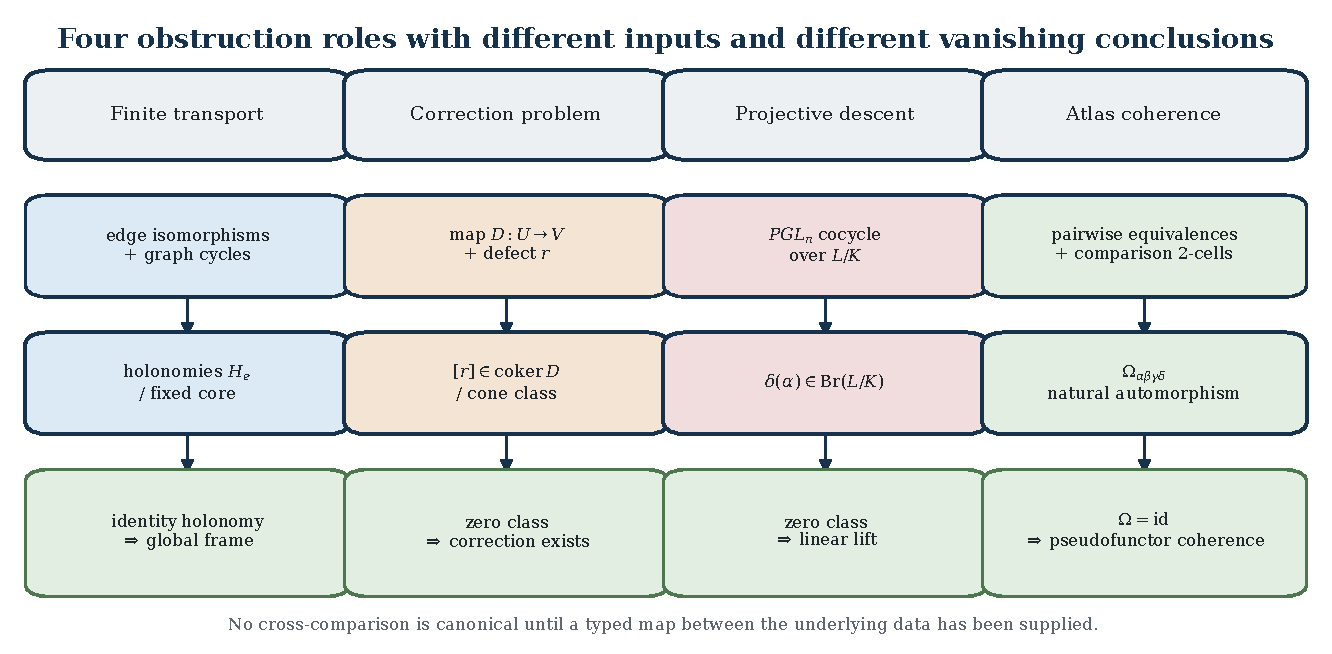
\includegraphics[width=0.99\textwidth]{obstruction_comparison.pdf}
\caption{Four obstruction pipelines.  The word \emph{obstruction} names a role, not one universal scalar.  The required input datum determines both the obstruction object and the exact consequence of vanishing.}
\label{fig:obstruction-comparison}
\end{figure}

\begin{resultbox}
\textbf{Section result.}
The atlas layer now has explicit stratum passports, normalized subcategories, representation groupoids, a directed transformation category, bridge classes, information-loss profiles, overlap and bridge-law certificates, and a concrete higher-coherence defect.  The four obstruction theories are stated with their own data and vanishing criteria.  Finite holonomy supplies a maximal path-flat core, split bridges expose reversible consistent cores inside directional maps, relative cokernels separate correction from coarsening loss, and Galois theory separates Hilbert-90 effectivity from Brauer and Tannakian boundaries.  The general heterogeneous atlas is still not declared effective until its actual bridge passports and coherence cells are verified.
\end{resultbox}


\section{The theorem concordance and edition control}

\subsection{Audit result}

The concordance contains 56 components. Thirty-eight are proved internally, eight are classical theorems imported and reinterpreted, two are proved conditionally, two are definition or framework rows, and six remain conjectural. The new foundations row records the finite profiled Universal Lane Transport Theorem. The conjectural entries remain concentrated in the cross-stratum assembly layer. The local packet, obstruction, Galois, sequence, and Mahler components are substantially more complete than an older open-question ledger suggests.

\begin{table}[t]
\centering
\caption{Status distribution in the 75-component theorem concordance.}
\label{tab:status-summary}
\small
\begin{tabular}{@{}lr@{}}
\toprule
Classification & Components\\
\midrule
\StatusInternal & 52\\
\StatusClassical & 12\\
\StatusConditional & 2\\
\StatusFramework & 3\\
\StatusConjectural & 6\\
\midrule
\textbf{Total} & \textbf{75}\\
\bottomrule
\end{tabular}
\end{table}

\begin{table}[t]
\centering
\caption{Concordance coverage by mathematical domain.}
\label{tab:domain-summary}
\small
\begin{tabular}{@{}lr@{}}
\toprule
Domain & Components\\
\midrule
Foundations & 17\\
Groupoids and descent & 7\\
Obstruction theory & 4\\
Galois stratum & 4\\
Linear stratum & 3\\
Holonomic stratum & 1\\
Digital stratum & 2\\
Algebraic stratum & 1\\
Transform stratum & 1\\
Product stratum & 1\\
Multiplicative stratum & 1\\
Local stratum & 3\\
Functional Mahler stratum & 3\\
Assembly & 9\\
Semantic quotient calculus & 7\\
Bridge loss calculus & 2\\
Carrier and observer change & 5\\
Convex and admissibility change & 3\\
Doctrine comparison & 1\\
\bottomrule
\end{tabular}
\end{table}


\subsection{Material supersession decisions}

Three corrections are mathematically consequential.

\paragraph{Relative obstruction theory.}
Older Paper III editions leave a broad universal packet-obstruction principle conjectural. The strengthened edition replaces the finite-projector formulation by the relative class \([r]\in\coker D\), with vanishing, naturality, packet decomposition, quotient projectors, relative exact sequences, and mapping-cone formulations proved for declared correction data \cite{P3,MIG}. The unresolved problem is not the quotient construction itself. It is a choice-free mechanism assigning the appropriate correction datum to arbitrary problems and strata.

\paragraph{Paper I edition policy.}
The complete symbolic core remains the theorem-ID and proof-status spine. The expanded clarified edition strengthens exposition and hypotheses without replacing the stable record identifiers \cite{P1}.

\paragraph{Core-Transfer status.}
Addendum 04 replaces the isolated \(m=6,d=3\) boundary by the exact composite-modulus rank law, sharp integral packet minimum, universal decoder, and all-degree stabilization \cite{CT4}. The former example is now a sharp negative control inside a general theorem.

\subsection{Existing bridges and exact invariant slices}

The strongest source edition already contains the following exact or effective bridges on declared domains:

\begin{itemize}
\item constant recurrence \(\leftrightarrow\) rational ordinary generating function \(\leftrightarrow\) finite linear state;
\item P-recursive \(\leftrightarrow\) D-finite coefficient translation;
\item finite digit realization \(\leftrightarrow\) finite \(k\)-kernel;
\item rational functional-Mahler mask \(\to\) Cartier representation \(\to\) finite automaton;
\item finite-mask Cartier transitions \(\leftrightarrow\) carry matrices;
\item selected algebraic branch \(\to\) packet polynomial system;
\item invertible transform \(\leftrightarrow\) transported packet resolution;
\item Euler-product exponent coordinates \(\leftrightarrow\) logarithmic-derivative recurrence data;
\item finite modular state \(\to\) local Newton-Mahler interpolation;
\item local Mahler coordinates \(\leftrightarrow\) affine polyphase branches;
\item finite resolved \(C^*\)-system \(\to\) faithful Hilbert packet realization.
\end{itemize}

The persistent C-finite stratum has the strongest complete transfer invariant. Active spectral and torsion-phase data determine the exact minimal recurrence, reduced denominator, Hankel rank, state dimension, rank drops, and periodic packet profile of every arithmetic subsequence \cite{SEQ}. Restricted exact coordinate systems also exist for fixed-radix automata, filtered Euler products, multiplicative prime-power seeds, local Mahler charts, finite semisimple Galois descent, and finite seed lattices. None of these restricted results is a single all-stratum classifier.

\begin{figure}[htbp]
\centering
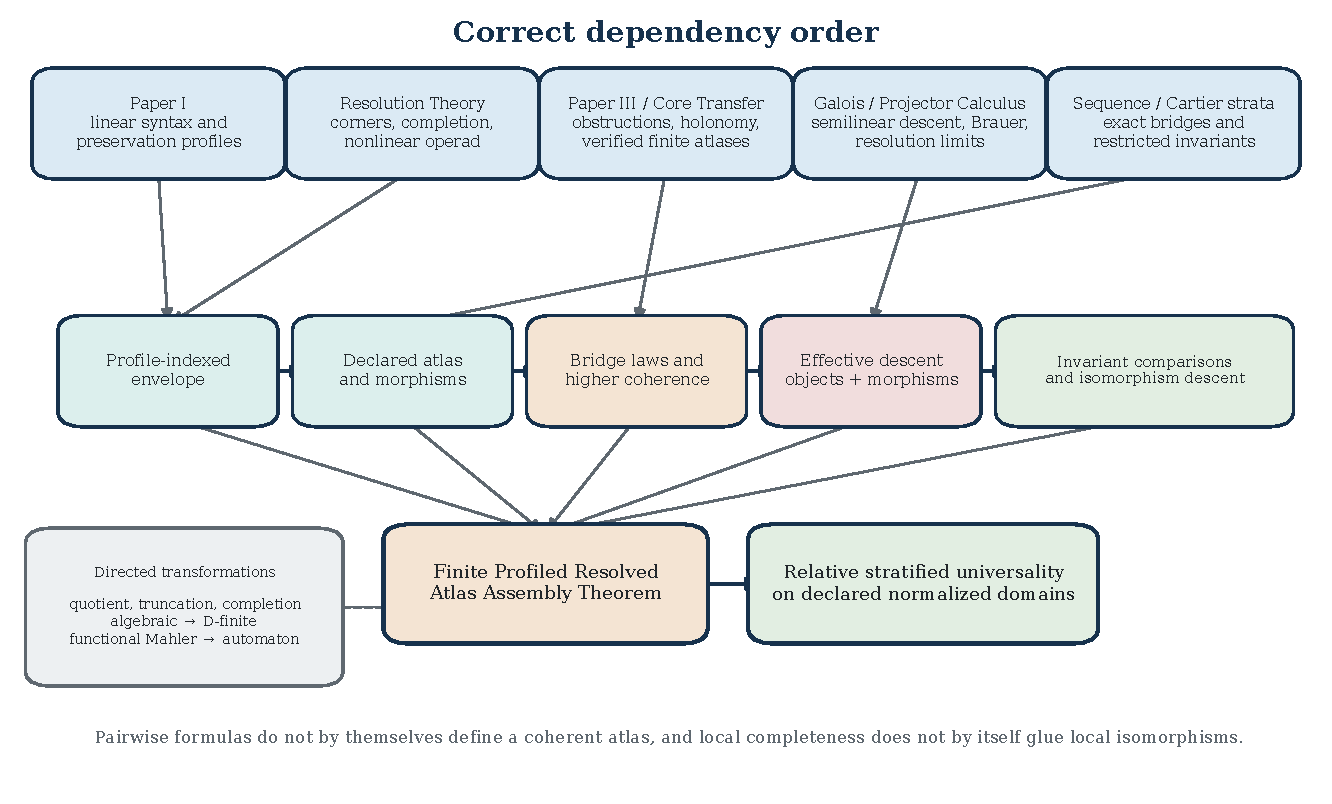
\includegraphics[width=0.98\textwidth]{dependency_graph.pdf}
\caption{The corrected dependency graph. The theorem concordance and local results feed the assembly theorem, but the heterogeneous conclusion still depends on explicit atlas construction, coherence, effectivity, and isomorphism descent.}
\label{fig:dependency-graph}
\end{figure}

\section{Finite profiled resolved atlas assembly}

\subsection{Finite atlases and descent data}

\begin{definition}[Finite profiled resolved atlas]
Fix a small resolved theory \(\bbK\). A finite profiled resolved atlas consists of:
\begin{enumerate}[label=\textup{(A\arabic*)}]
\item a finite indexing category \(\check{\mathcal A}\), retained through the overlap degrees needed for the cocycle law;
\item a pseudofunctor
\[
\mathfrak R:\check{\mathcal A}^{\mathrm{op}}\to\Cat;
\]
\item a declared preservation profile \(\Pi_U\) on every chart and overlap category \(\mathfrak R(U)\);
\item coherent equivalences on the reversible overlaps and separately typed directional transformations;
\item a pseudonatural semantics
\[
\Sem:\mathfrak R\Rightarrow\mathfrak O
\]
into a common observable doctrine;
\item optional pseudonatural invariant families with explicitly typed comparison cells.
\end{enumerate}
\end{definition}

\begin{definition}[Descent category]
The category \(\Desc(\mathfrak R)\) has pseudocones over \(\mathfrak R\) as objects and modifications as morphisms. Concretely, an object is a compatible family
\[
(M_\alpha,\theta_{\alpha\beta})
\]
with invertible overlap comparisons satisfying the cocycle law. A morphism is a compatible family of chart morphisms.
\end{definition}

\subsection{The assembly theorem}

\begin{theorem}[Finite profiled resolved atlas assembly]
\label{thm:atlas-assembly}
Let
\[
\mathfrak R:\check{\mathcal A}^{\mathrm{op}}\to\Cat
\]
be a finite profiled resolved atlas. Assume the chart and overlap categories are small, or locally small in one fixed universe, the reversible transitions and comparison cells satisfy the pseudofunctor coherence equations, and every construction used below belongs to the verified profile of every participating chart and bridge. Then:

\begin{enumerate}[label=\textup{(\roman*)}]
\item \(\Desc(\mathfrak R)\) exists and has the universal property of the finite pseudolimit of \(\mathfrak R\).
\item There is a canonical equivalence
\[
\Core\bigl(\Desc(\mathfrak R)\bigr)
\simeq
\Desc\bigl(\mathfrak R^{\simeq}\bigr).
\]
\item Every pseudonatural transformation \(T:\mathfrak R\Rightarrow\mathfrak S\) induces a functor
\[
\Desc(T):\Desc(\mathfrak R)\to\Desc(\mathfrak S).
\]
If every \(T_U\) is an equivalence, then \(\Desc(T)\) is an equivalence. A pointwise noninvertible \(T\) remains directional.
\item If two global morphism expressions use only constructors in the common verified preservation profile and their equality is proved in the resolved syntax, then, after every domain-specific hypothesis is verified locally, their realizations are equal in \(\Desc(\mathfrak R)\).
\item A coherent pseudonatural invariant family \(I:\mathfrak R\Rightarrow\mathfrak V\) induces
\[
\Desc(I):\Desc(\mathfrak R)\to\Desc(\mathfrak V).
\]
\item If every local invariant is complete on its normalized chart and the groupoid of local invariant-compatible isomorphisms has effective descent, then \(\Desc(I)\) is complete on the corresponding global normalized category.
\end{enumerate}

If the semantic pseudonatural transformation is effective for objects and morphisms, then \(\Desc(\Sem)\) identifies descent data with the declared global semantic objects.
\end{theorem}

\begin{proof}
Objects and morphisms of \(\Desc(\mathfrak R)\) are finite compatible families. Identities and composition are defined componentwise. The pseudofunctor coherence equations ensure that componentwise composition remains compatible. This explicit construction has the universal property of pseudocones, proving (i).

A descent morphism is invertible exactly when each component is invertible. The componentwise inverses satisfy the overlap equations obtained by inverting the original equations. This proves (ii).

A pseudonatural transformation acts on chart objects, overlap comparisons, and chart morphisms componentwise. Its coherence cells supply the target cocycle law. Pointwise quasi-inverses and their modifications descend, proving (iii).

For (iv), the equational realization principle transports the proof to each chart because every constructor used by the proof is preserved. Bridge naturality makes the local equalities compatible on overlaps. Equality in the descent category is componentwise. The argument creates no missing analytic or arithmetic hypotheses.

Statement (v) is the same pseudonatural-transformation construction applied to the invariant family. For (vi), an isomorphism between descended invariants gives local invariant matches. Local completeness supplies local object isomorphisms. The added isomorphism-effectivity hypothesis is exactly what glues those local isomorphisms to a global one. Without it, a holonomy class, a relative cokernel class, a Brauer class, or a higher coherence defect may obstruct the gluing.

The final assertion is the definition of semantic effectivity applied to the induced descent functor.
\end{proof}

\begin{corollary}[No automatic promotion of directional bridges]
A directional bridge contributes a global functor only when it is pseudonatural with respect to the chosen atlas. It contributes an equivalence only when the chartwise bridge is an equivalence on the named overlap. No quotient, completion, or compression becomes reversible merely because it appears in the same diagram.
\end{corollary}

\begin{corollary}[Global theorem transport]
A theorem proved from packet reconstruction, refinement, residual calculus, or another preserved constructor descends globally only when every chart and bridge used by the proof carries that constructor in its verified preservation profile.
\end{corollary}

\begin{remark}[Exact status]
\Cref{thm:atlas-assembly} is a proved conditional theorem. It does not prove that the full proposed Komorebi atlas satisfies the hypotheses. The remaining work is the verification of the actual profiles, overlap categories, naturality cells, higher coherence, and effectivity.
\end{remark}

\part{Certified native strata}

\section{Verified finite Mahler atlas models}

Two exact finite models already realize substantial pieces of the assembly theorem. They remain inside the affine-Mahler and packet-analysis setting, but they verify nontrivial coherence and effectivity mechanisms.

\subsection{Affine-Mahler chart groupoid}

Fix \(d\ge0\). Over characteristic zero, the affine Mahler coefficient maps \(A_{m,s}^{(d)}\) are invertible and satisfy
\[
A_{n,t}^{(d)}A_{m,s}^{(d)}=A_{mn,mt+s}^{(d)}.
\]
For coprime \(m,n\), the two paths around every declared Chinese-remainder diamond are equal \cite{CT4}. Hence every finite subdiagram generated by these charts is a coherent finite chart groupoid with trivial holonomy on those diamonds.

\begin{proposition}[Rational affine-Mahler chart groupoid]
Every finite characteristic-zero diagram generated by the invertible affine Mahler charts and the declared CRT comparison cells defines a strict finite groupoid atlas. Its path transport depends only on the represented affine substitution, and every declared CRT cycle has identity holonomy.
\end{proposition}

\subsection{Integral split packet descent}

Let
\[
A=P_{m,S}^{(d)}:\mathbb Z^{d+1}\to\mathbb Z^{|S|(d+1)}
\]
be a stacked affine-Mahler packet analysis map. Whenever an integer left inverse \(L\) exists,
\[
LA=I,
\qquad
\Pi=AL,
\qquad
\Pi^2=\Pi,
\]
and
\[
\mathbb Z^{|S|(d+1)}=\im A\oplus\ker L.
\]
Thus the source chart and the normalized packet core \(\im A\) are equivalent, while \(\ker L\) is a named residual rather than discarded information.

Addendum 04 proves that the prefix
\[
S_*=\{0,1,\dots,L_{\mathbb Z}(m,d)-1\}
\]
with
\[
L_{\mathbb Z}(m,d)=\min(d+1,B(m)),
\qquad
B(m)=\max\bigl(\{1\}\cup\{p^{v_p(m)}:p\mid m\}\bigr),
\]
always admits an integer decoder and is cardinality-minimal \cite{CT4}.

\begin{proposition}[Integral split Mahler packet descent]
The analysis-decoder pair above gives effective object and morphism descent between the source chart and the normalized packet-core chart. The split identity survives every base change. The residual summand \(\ker L\) is functorial under maps intertwining both \(A\) and \(L\).
\end{proposition}

\begin{proof}
The identities \(LA=I\) and \(\Pi=AL\) show that \(A\) identifies the source with \(\im A\), with inverse \(L|_{\im A}\). For any packet vector \(y\),
\[
y=ALy+(y-ALy),
\]
where \(ALy\in\im A\) and \(y-ALy\in\ker L\). The intersection is zero because \(Ax\in\ker L\) implies \(x=LAx=0\). Tensoring \(LA=I\) with any coefficient ring preserves the split identity. Intertwining maps preserve the image and kernel decompositions.
\end{proof}

\begin{figure}[htbp]
\centering
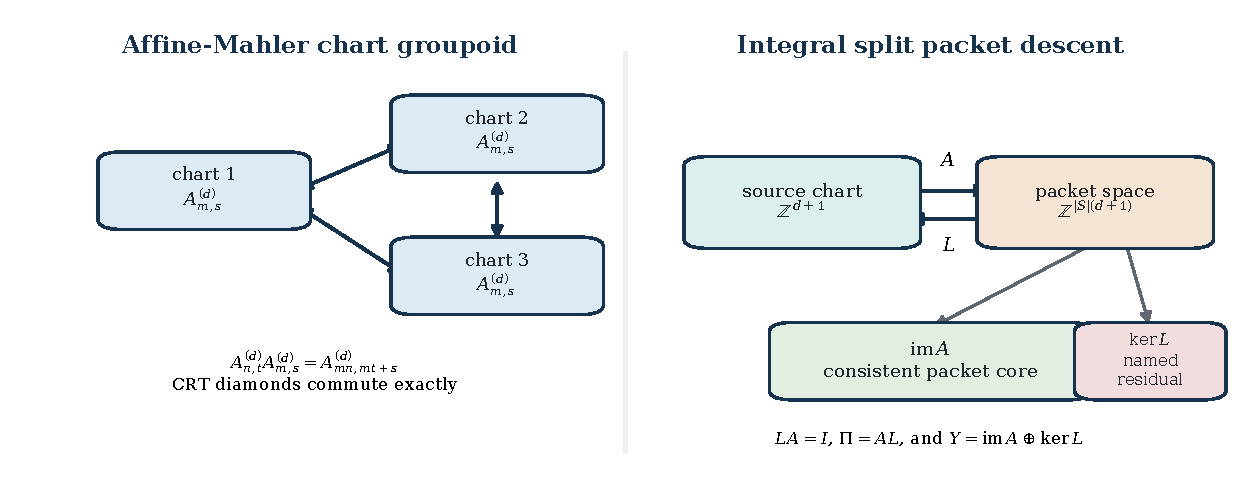
\includegraphics[width=0.98\textwidth]{mahler_models.pdf}
\caption{Two verified finite atlas mechanisms. The first is reversible and coherent. The second is split analysis-synthesis with a retained residual.}
\label{fig:mahler-models}
\end{figure}

\section{The normalized C-finite three-chart atlas}

This section completes the first cross-presentation model in the theorem dependency graph. It does not combine unrelated broad strata, but it does prove a genuine three-chart effective descent theorem with nontrivial morphisms on the state side.

\subsection{Persistent C-finite semantics}

Fix a field \(K\). A nonzero C-finite sequence \(a=(a_n)_{n\ge0}\) is \emph{persistent} when its minimal characteristic polynomial has nonzero constant term. Equivalently, its active characteristic roots are nonzero, or its minimal state transition is invertible \cite{SEQ}.

Let \(\Seq_K^{\mathrm{pers}}\) be the discrete groupoid of persistent C-finite sequences over \(K\).

\subsection{The recurrence chart}

An object of \(\Rec_K^{\mathrm{min}}\) is a pair
\[
(\chi,\mathbf a_0),
\]
where
\[
\chi(x)=x^d-c_{d-1}x^{d-1}-\cdots-c_1x-c_0,
\qquad c_0\ne0,
\]
is the monic minimal recurrence polynomial and \(\mathbf a_0=(a_0,\dots,a_{d-1})\) is the initial vector. It generates the sequence
\[
a_{n+d}=c_{d-1}a_{n+d-1}+\cdots+c_1a_{n+1}+c_0a_n.
\]
Because the recurrence is normalized and minimal, two objects representing the same sequence are equal. Thus \(\Rec_K^{\mathrm{min}}\) is a discrete groupoid.

\subsection{The rational OGF chart}

An object of \(\Rat_K^{\mathrm{red}}\) is a reduced rational power series
\[
A(z)=\frac{P(z)}{Q(z)},
\qquad
Q(0)=1,
\qquad
\gcd(P,Q)=1,
\qquad
\deg P<\deg Q,
\]
whose reciprocal characteristic polynomial has nonzero constant term. Again the normalized reduced form is unique, so \(\Rat_K^{\mathrm{red}}\) is discrete.

The recurrence-to-OGF bridge is explicit. From
\[
\chi(x)=x^d-c_{d-1}x^{d-1}-\cdots-c_0
\]
set
\[
Q(z)=z^d\chi(z^{-1})
=1-c_{d-1}z-\cdots-c_0z^d.
\]
The numerator is the degree-\(<d\) truncation of \(Q(z)\sum_{n\ge0}a_nz^n\). Conversely, clearing \(Q\) recovers the recurrence and the initial vector. Minimality is equivalent to reducedness.

\subsection{The minimal state chart}

An object of \(\State_K^{\mathrm{min}}\) is a triple
\[
(C,v,\lambda),
\qquad
C\in M_d(K),\quad v\in K^d,\quad \lambda\in(K^d)^*,
\]
with \(C\) invertible, producing
\[
a_n=\lambda C^nv,
\]
and satisfying reachability and observability. A morphism
\[
S:(C,v,\lambda)\longrightarrow(C',v',\lambda')
\]
is a similarity satisfying
\[
C'=SCS^{-1},
\qquad
v'=Sv,
\qquad
\lambda'=\lambda S^{-1}.
\]
The semantic functor sends a state to its coefficient sequence.

The state-to-OGF bridge is the resolvent
\[
A(z)=\lambda(I-zC)^{-1}v.
\]
The reduced denominator has degree equal to the minimal state dimension, which equals the Hankel rank. Conversely, a reduced rational OGF has a companion realization. Reducedness makes the companion realization reachable, while the companion output is observable. Any two minimal realizations of the same sequence are uniquely similar through their common shift action on the Hankel column space \cite{SEQ}.

\subsection{Effective descent across the three charts}

\begin{theorem}[Normalized C-finite three-chart atlas]
\label{thm:cfinite-three-chart}
For every field \(K\), the semantic functors fit into equivalences of groupoids
\[
\Rec_K^{\mathrm{min}}
\simeq
\Rat_K^{\mathrm{red}}
\simeq
\State_K^{\mathrm{min}}
\simeq
\Seq_K^{\mathrm{pers}}.
\]
The recurrence-rational bridge is a strict inverse pair. The rational-state bridge is an equivalence with companion quasi-inverse. The comparison isomorphism on the state-side composite is the unique similarity between minimal realizations. Consequently:

\begin{enumerate}[label=\textup{(\roman*)}]
\item the three charts and their pairwise overlaps form a coherent finite profiled atlas;
\item the triple-overlap comparison satisfies the cocycle law by uniqueness of minimal similarity;
\item descent for objects and morphisms is effective;
\item the descent category is equivalent to \(\Seq_K^{\mathrm{pers}}\).
\end{enumerate}
\end{theorem}

\begin{proof}
The equivalence between normalized minimal recurrences and reduced rational ordinary generating functions follows from the explicit reciprocal-denominator formula and clearing of the denominator. These constructions are mutually inverse.

A minimal state gives a rational resolvent. Conversely, a reduced rational series gives a companion state. Minimal linear dimension equals Hankel rank, and the reduced denominator degree has the same value. Hence the companion state is minimal. Any two minimal states representing the same sequence identify with the forward shift on the Hankel column space and are therefore similar. The similarity is unique because a reachable state is spanned by \(C^nv\), so an intertwiner fixing the input vector is determined on a spanning set.

Choose the recurrence-to-state bridge to be the companion realization obtained through the rational chart. Then one triangular composite is strict. On the state side, the composite through the rational and recurrence charts returns the companion realization of the same sequence. The unique minimal similarity supplies the comparison isomorphism. Any two composites around a triple overlap are comparison isomorphisms between the same minimal realizations, so uniqueness forces the cocycle law.

Each semantic functor is an equivalence to the same discrete groupoid of persistent sequences. Compatible local objects and morphisms therefore descend uniquely up to the stated similarity, proving effectivity and the final equivalence.
\end{proof}

\begin{figure}[htbp]
\centering
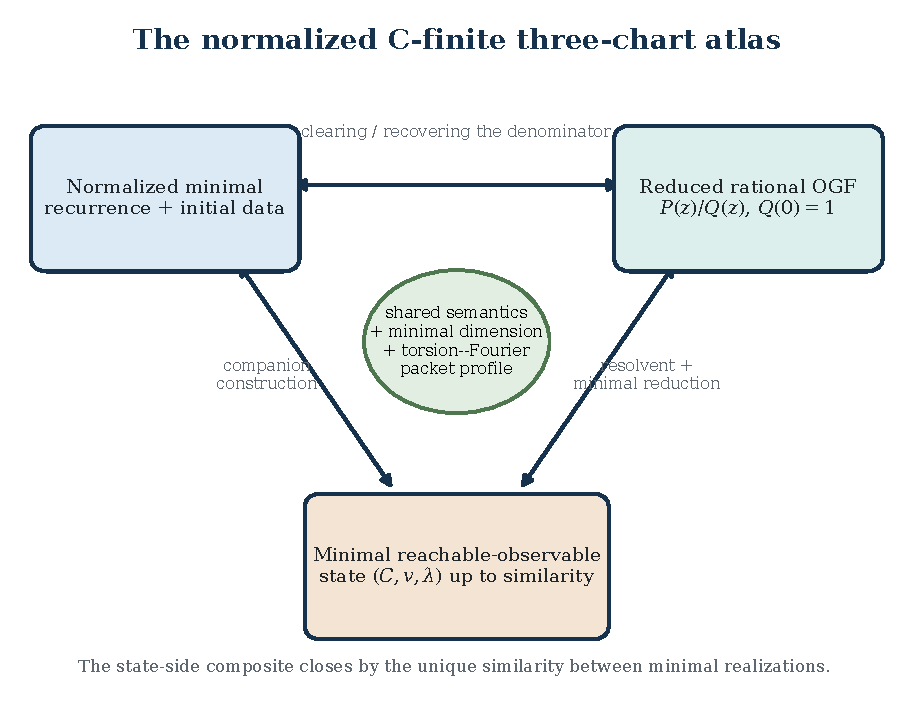
\includegraphics[width=0.82\textwidth]{cfinite_triangle.pdf}
\caption{The normalized C-finite atlas. The recurrence and rational charts are canonical normal forms. The state chart has nontrivial presentation coordinates, but minimality makes every semantic identification unique up to similarity.}
\label{fig:cfinite-triangle}
\end{figure}

\subsection{Descent of the minimality and torsion-Fourier invariants}

For a persistent C-finite sequence, the minimal dimension
\[
\rho(a)=\linrank(a)=\rank H(a)
\]
is simultaneously the minimal recurrence order, the reduced denominator degree, and the dimension of a minimal reachable-observable state.

Over characteristic zero, write the unique active expansion over an algebraic closure as
\[
a_n=\sum_{\lambda\in\Lambda}P_\lambda(n)\lambda^n.
\]
For each sampling modulus \(N\) and address \(j\), the spectral torsion-Fourier theorem computes the exact minimal recurrence, reduced denominator, Hankel rank, state dimension, rank-drop mechanism, and finite periodic packet signature of \(a_{Nm+j}\) \cite{SEQ}.

\begin{corollary}[Cross-presentation torsion-Fourier descent]
The minimal dimension and the complete arithmetic-subsequence packet-complexity profile are independent of whether the input is supplied as a normalized minimal recurrence, a reduced rational OGF, or a minimal state realization. The exact compiler outputs agree under every bridge in \cref{thm:cfinite-three-chart}.
\end{corollary}

\begin{proof}
All three charts represent the same sequence. The compiler theorem accepts any of the three presentation types and computes quantities determined by the active modal decomposition or, equivalently, by exact reachable-observable reduction of the jump state. The bridge functors preserve the coefficient sequence, so the outputs agree.
\end{proof}

The phrase ``complete invariant'' here has a declared target. The torsion-Fourier signature is complete for the minimal recurrence and complexity profile of every arithmetic subsequence. It is not asserted to classify arbitrary sequence presentations or all sequence phenomena.

\subsection{Exact examples}

\begin{table}[htbp]
\centering
\caption{Three exact C-finite examples across the normalized atlas.}
\label{tab:cfinite-examples}
\small
\begin{tabularx}{\textwidth}{@{}L{0.18\textwidth}L{0.19\textwidth}L{0.19\textwidth}L{0.15\textwidth}Y@{}}
\toprule
Sequence & Minimal recurrence & Reduced OGF & Minimal dimension & Packet behavior\\
\midrule
Fibonacci \(F_n\) & \(x^2-x-1\) & \(z/(1-z-z^2)\) & \(2\) & The root ratio is not torsion. Every arithmetic subsequence retains rank \(2\).\\
\(1+(-1)^n\) & \(x^2-1\) & \(2/(1-z^2)\) & \(2\) & At \(N=2\), the even packet is constant of rank \(1\) and the odd packet is zero.\\
\(n+1)\) & \((x-1)^2\) & \(1/(1-z)^2\) & \(2\) & Every packet remains a nonzero affine polynomial in the packet index and retains rank \(2\).\\
\bottomrule
\end{tabularx}
\end{table}

\section{A first heterogeneous effective-descent atlas}
\label{sec:periodic-heterogeneous-atlas}

The previous sections separated the formal assembly theorem from the nonformal work of declaring and verifying an actual atlas.  This section discharges that burden for a deliberately restricted but genuinely heterogeneous example.  The charts do not merely use different coordinates inside one linear category.  They belong to three of the principal strata:
\[
\text{finite linear and C-finite}
\qquad
\text{digital and automatic}
\qquad
\text{functional-Mahler and Cartier}.
\]
The common semantic objects are unit purely periodic sequences over a prime field.  The restriction is strong enough to make every bridge explicit, every normalized fiber rigid, every nonempty triple overlap coherent, and descent effective for both objects and morphisms.  At the same time it is broad enough to contain repeated-root recurrences in characteristic \(p\), nontrivial minimal automata, rational functional-Mahler masks, and redundant Cartier compiler presentations.

\subsection{The restricted semantic doctrine}

Fix a prime \(p\).  Let \(\Per_p^{\times,\mathrm{per}}\) denote the discrete category whose objects are sequences
\[
a=(a_n)_{n\geq 0}\in \mathbb F_p^{\mathbb N}
\]
satisfying
\[
a_0=1
\qquad\text{and}\qquad
 a_{n+T}=a_n
\quad(n\geq 0)
\]
for some \(T\geq 1\).  The least such positive integer is the \emph{minimal period} \(T(a)\).  Write
\[
w(a)=(a_0,\ldots,a_{T(a)-1})
\]
for the primitive period word and
\[
W_a(z)=\sum_{r=0}^{T(a)-1}a_rz^r.
\]
Then
\begin{equation}
\label{eq:periodic-ogf-unreduced}
F_a(z)=\sum_{n\geq 0}a_nz^n
=
\frac{W_a(z)}{1-z^{T(a)}}.
\end{equation}
The fraction in \cref{eq:periodic-ogf-unreduced} need not be reduced.  Cancellation is part of the normalized rational chart rather than an error.  For example, over \(\mathbb F_3\), the period word \(12\) has
\[
\frac{1+2z}{1-z^2}=\frac{1}{1+z}.
\]

\begin{boundary}[Why the unit condition is retained]
The functional-Mahler bridge uses the formal quotient
\[
R_a(z)=\frac{F_a(z)}{F_a(z^p)}.
\]
It is regular at the origin exactly when \(F_a(0)\neq 0\).  The normalization \(a_0=1\) removes scalar ambiguity and gives \(R_a(0)=1\).  Purely periodic sequences with \(a_0=0\) remain valid C-finite and automatic objects, but they need not lie in this regular unit-mask overlap.  They are not discarded; they lie outside the selected heterogeneous atlas.
\end{boundary}

\begin{proposition}[Finite-field persistence equals pure periodicity]
\label{prop:persistent-periodic}
For a sequence over \(\mathbb F_p\), the following are equivalent.
\begin{enumerate}[label=\textup{(\roman*)}]
\item The sequence is C-finite and its minimal recurrence has nonzero constant term.
\item The sequence has a finite-dimensional state realization
\[
a_n=\lambda C^nv
\]
with \(C\in GL_d(\mathbb F_p)\).
\item The sequence is purely periodic from \(n=0\).
\end{enumerate}
If \(m_a(x)\) is the monic minimal recurrence polynomial and \(T=T(a)\), then
\begin{equation}
\label{eq:minimal-period-annihilator}
m_a(x)\mid x^T-1,
\qquad
T=\min\{N\geq 1:m_a(x)\mid x^N-1\}.
\end{equation}
\end{proposition}

\begin{proof}
A recurrence with nonzero constant term has an invertible companion matrix, giving (i) \(\Rightarrow\) (ii).  The orbit of \(v\) under an invertible map of the finite set \(\mathbb F_p^d\) is a cycle containing its initial state, so (ii) \(\Rightarrow\) (iii).  A sequence of period \(T\) is annihilated by \(E^T-I\), where \(E\) is the forward shift, giving (iii) \(\Rightarrow\) (i).  The minimal annihilator divides every annihilator, hence \(m_a\mid x^T-1\).  Conversely, if \(m_a\mid x^N-1\), then \(E^N-I\) annihilates the sequence.  Minimality of \(T\) proves \cref{eq:minimal-period-annihilator}.
\end{proof}

Let
\[
F_a(z)=\frac{P_a(z)}{Q_a(z)}
\]
be reduced with
\[
P_a(0)=Q_a(0)=1.
\]
If \(d=\deg m_a\), then
\[
Q_a(z)=z^dm_a(z^{-1}),
\]
with the evident coefficient normalization.  Taking reciprocal polynomials in \cref{eq:minimal-period-annihilator} gives
\begin{equation}
\label{eq:minimal-period-denominator}
Q_a(z)\mid 1-z^T,
\qquad
T=\min\{N\geq 1:Q_a(z)\mid 1-z^N\}.
\end{equation}
Thus pure periodicity is visible both in the linear annihilator and in the reduced rational denominator.

\subsection{Four normalized charts}

The reversible core of the selected atlas has four charts.  Each chart carries its own native objects and morphisms, but every normalized fiber over a fixed sequence will be shown to be contractible.

\subsubsection{The minimal recurrence chart}

An object of \(\Rec_p^{\times,\mathrm{per}}\) is the normalized minimal recurrence polynomial
\[
m(x)=x^d+c_1x^{d-1}+\cdots+c_d,
\qquad c_d\neq 0,
\]
together with the initial vector \((a_0,\ldots,a_{d-1})\), subject to \(a_0=1\) and the requirement that the generated sequence is purely periodic.  Minimality means that no monic recurrence of lower degree annihilates the sequence.  Morphisms are recurrence-presentation isomorphisms preserving the coefficient sequence.  Because the minimal annihilator and initial data are unique, every endomorphism is the identity.

\subsubsection{The reduced rational chart}

An object of \(\Rat_p^{\times,\mathrm{per}}\) is a reduced fraction
\[
F(z)=\frac{P(z)}{Q(z)}\in\mathbb F_p(z),
\qquad
P(0)=Q(0)=1,
\]
whose coefficient sequence is purely periodic.  Equivalently, \(Q\mid 1-z^T\) for some \(T\) and the reduced coefficient sequence has no transient prefix.  Morphisms preserve the rational function.  Reducedness and the constant-term normalization make this chart rigid.

The recurrence-rational bridge is the strict inverse pair already used in the C-finite atlas: multiply the generating series by the reciprocal recurrence denominator, or recover the recurrence by clearing the reduced denominator.  On the present finite-field subcategory, the additional condition \(Q\mid1-z^T\) records pure periodicity.

\subsubsection{The canonical digital chart}

For \(0\leq d<p\), define the Cartier section of a sequence by
\[
(\Lambda_da)_n=a_{pn+d}.
\]
The \(p\)-kernel is
\begin{equation}
\label{eq:p-kernel}
\mathcal K_p(a)
=
\left\{
\Lambda_{d_{\ell-1}}\cdots\Lambda_{d_0}a:
\ell\geq 0,\ 0\leq d_i<p
\right\}.
\end{equation}
We use least-significant-digit-first words.  Every finite digit word is allowed.  Appending high zero digits may change the internal state but never changes the represented coefficient, because the output of a state \(b\) is \(b_0\) and \((\Lambda_0b)_0=b_0\).

The canonical Moore automaton has state set \(\mathcal K_p(a)\), start state \(a\), transition
\[
\delta_d(b)=\Lambda_db,
\]
and output
\[
o(b)=b_0.
\]
After reading \(d_0,\ldots,d_{\ell-1}\), its state is
\[
\Lambda_{d_{\ell-1}}\cdots\Lambda_{d_0}a
=
\bigl(n\longmapsto a_{p^\ell n+r}\bigr),
\qquad
r=\sum_{j=0}^{\ell-1}d_jp^j.
\]

\begin{proposition}[Finite periodic kernel and exact state model]
\label{prop:periodic-kernel}
Let \(a\in\Per_p^{\times,\mathrm{per}}\) have minimal period \(T\) and period word \(w\).  Every kernel state has the form
\begin{equation}
\label{eq:periodic-kernel-state}
b_{u,r}(n)=w_{un+r\bmod T},
\qquad
u\in U_p(T),\quad r\in\mathbb Z/T\mathbb Z,
\end{equation}
where
\[
U_p(T)=\{p^e\bmod T:e\geq 0\}.
\]
The digit transition on pair representatives is
\begin{equation}
\label{eq:pair-transition}
(u,r)\xrightarrow{d}(pu,r+ud)\pmod T,
\end{equation}
and the output is \(w_r\).  Quotienting pair representatives by equality of the sequences in \cref{eq:periodic-kernel-state} gives the canonical minimal least-significant-digit-first \(p\)-DFAO for \(a\).
\end{proposition}

\begin{proof}
After \(\ell\) digits, the resulting subsequence is \(n\mapsto a_{p^\ell n+r}\), which depends only on \((p^\ell\bmod T,r\bmod T)\).  Applying \(\Lambda_d\) gives
\[
\Lambda_db_{u,r}(n)
=b_{u,r}(pn+d)
=w_{(pu)n+(r+ud)},
\]
proving \cref{eq:pair-transition}.  The pair set is finite, so the kernel is finite.  Every kernel state is reachable by construction.  If two kernel sequences differ, they differ at some \(n\); reading the base-\(p\) digits of that \(n\) distinguishes the states by their outputs.  Hence the kernel automaton is minimal.  Any other reachable minimal automaton producing the same sequence is uniquely isomorphic to it by the usual behavioral quotient.
\end{proof}

The pair model gives a useful finite bound.  Write
\[
T=p^\nu M,
\qquad
\gcd(M,p)=1,
\]
and set \(\operatorname{ord}_1(p)=1\).

\begin{lemma}[Exact multiplier-orbit size]
\label{lem:multiplier-orbit-size}
The set \(U_p(T)\) has cardinality
\begin{equation}
\label{eq:u-size}
|U_p(T)|
=
\nu+\operatorname{ord}_M(p).
\end{equation}
Consequently,
\begin{equation}
\label{eq:kernel-state-bound}
|\mathcal K_p(a)|
\leq
T\bigl(\nu+\operatorname{ord}_M(p)\bigr).
\end{equation}
\end{lemma}

\begin{proof}
For \(0\leq e<\nu\), the residues \(p^e\bmod p^\nu\) have distinct \(p\)-adic valuations.  For \(e\geq\nu\), the residue is zero modulo \(p^\nu\), while modulo \(M\) it runs through one multiplicative cycle of length \(\operatorname{ord}_M(p)\).  The early and eventual residues cannot coincide.  This proves \cref{eq:u-size}.  The kernel is a quotient of the pair set \(U_p(T)\times\mathbb Z/T\mathbb Z\), giving \cref{eq:kernel-state-bound}.
\end{proof}

Let \(\Aut_p^{\times,\mathrm{per}}\) be the groupoid of reachable minimal least-significant-digit-first \(p\)-DFAOs whose output sequence lies in \(\Per_p^{\times,\mathrm{per}}\).  Morphisms are automaton isomorphisms preserving the start state, transitions, and outputs.  Reachability forces every automorphism to be the identity.

\subsubsection{The rational functional-Mahler mask chart}

For a unit formal series \(F(0)=1\), define its local functional-Mahler mask by
\begin{equation}
\label{eq:unique-local-mask}
\mathcal M_p(F)(z)
=
\frac{F(z)}{F(z^p)}.
\end{equation}
Then
\begin{equation}
\label{eq:functional-mahler-equation}
F(z)=\mathcal M_p(F)(z)F(z^p).
\end{equation}
Iterating \cref{eq:functional-mahler-equation} gives the coefficientwise product
\begin{equation}
\label{eq:mask-product}
F(z)
=
\prod_{j\geq0}\mathcal M_p(F)(z^{p^j}).
\end{equation}
Only finitely many factors contribute to each fixed coefficient.

If \(F=P/Q\) is reduced and unit normalized, then
\begin{equation}
\label{eq:rational-mask-formula}
R_F(z)
=
\frac{P(z)Q(z^p)}{Q(z)P(z^p)}.
\end{equation}
Thus every object of \(\Rat_p^{\times,\mathrm{per}}\) has a rational mask.  Reduce \cref{eq:rational-mask-formula} to
\[
R_F(z)=\frac{A(z)}{B(z)},
\qquad
A(0)=B(0)=1,
\qquad
\gcd(A,B)=1.
\]

Define \(\Mask_p^{\times,\mathrm{per}}\) to be the groupoid of such reduced rational masks whose normalized product solution \cref{eq:mask-product} has purely periodic coefficients.  Morphisms preserve the reduced mask.

\begin{theorem}[Unit rational functional-Mahler equivalence]
\label{thm:unit-rational-mask-equivalence}
The assignments
\[
F\longmapsto \frac{F(z)}{F(z^p)}
\qquad\text{and}\qquad
R\longmapsto \prod_{j\geq0}R(z^{p^j})
\]
are inverse equivalences
\[
\Rat_p^{\times,\mathrm{per}}
\simeq
\Mask_p^{\times,\mathrm{per}}.
\]
The mask is unique for the represented series.
\end{theorem}

\begin{proof}
Starting with \(F\), the finite product through level \(N\) telescopes:
\[
\prod_{j=0}^{N}\frac{F(z^{p^j})}{F(z^{p^{j+1}})}
=
\frac{F(z)}{F(z^{p^{N+1}})}.
\]
As \(N\to\infty\), the denominator converges coefficientwise to \(F(0)=1\), proving that the product recovers \(F\).  Conversely, the product solution satisfies \(F(z)=R(z)F(z^p)\), so \(R=F/F(z^p)\).  Reduced normalization makes the rational mask unique.
\end{proof}

\begin{boundary}[Functional Mahler is not Newton-Mahler]
The mask equation in this section is
\[
F(z)=R(z)F(z^p).
\]
It is a digit-section and automaton construction.  It is not the Newton-Mahler interpolation expansion
\[
f(x)=\sum_rc_r\binom{x}{r}.
\]
Both occur elsewhere in the Library, but this atlas uses only the functional-Mahler meaning.
\end{boundary}

\begin{figure}[htbp]
\centering
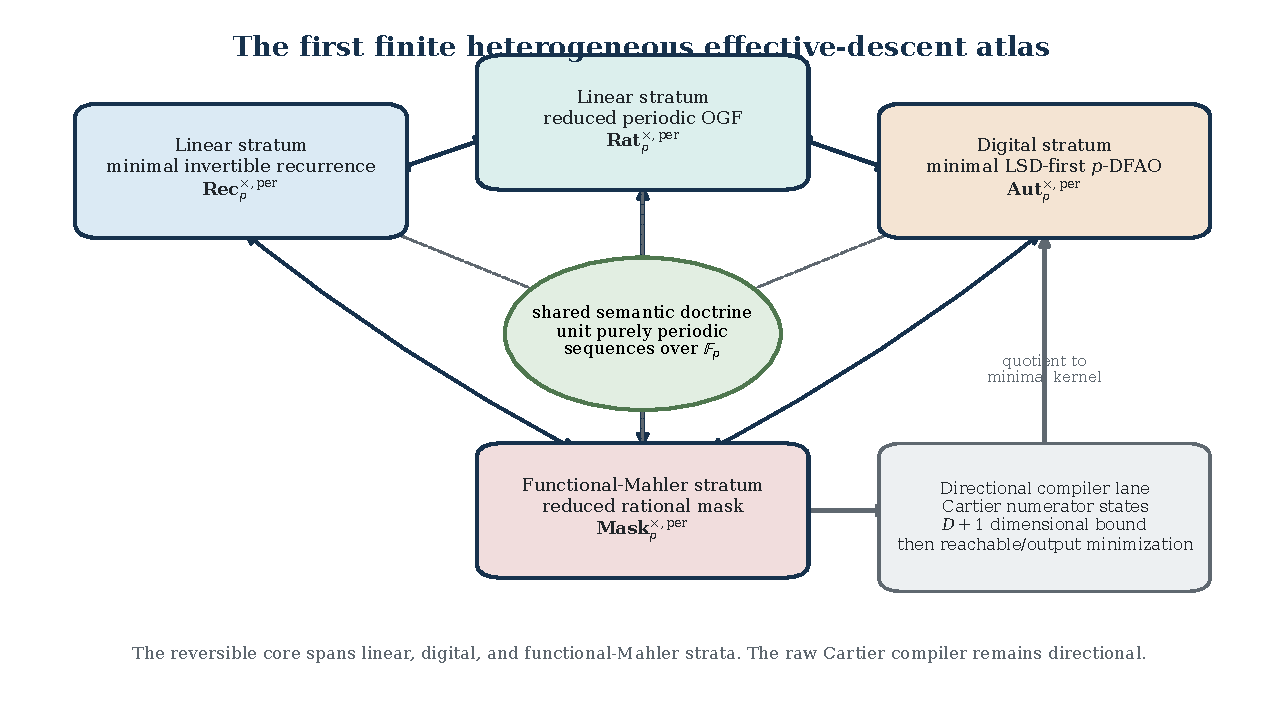
\includegraphics[width=0.99\textwidth]{periodic_heterogeneous_atlas.pdf}
\caption{The first heterogeneous atlas proved effective in this manuscript.  Four normalized reversible charts span three strata.  The raw Cartier compiler is retained as a directional lane because its numerator coordinates need not be minimal.}
\label{fig:periodic-heterogeneous-atlas}
\end{figure}

\subsection{Explicit bridge passports}

The reversible bridge core is generated by three explicit constructions:
\[
\Rec_p^{\times,\mathrm{per}}
\leftrightarrow
\Rat_p^{\times,\mathrm{per}},
\qquad
\Rat_p^{\times,\mathrm{per}}
\leftrightarrow
\Aut_p^{\times,\mathrm{per}},
\qquad
\Rat_p^{\times,\mathrm{per}}
\leftrightarrow
\Mask_p^{\times,\mathrm{per}}.
\]
The remaining reversible bridges are their normalized composites.  A separate constructor and reachable-restriction lane connects masks to the digital normal form through the Cartier compiler.

\begin{landscape}
\begin{longtable}{@{}L{0.13\linewidth}L{0.14\linewidth}L{0.14\linewidth}L{0.14\linewidth}L{0.15\linewidth}L{0.21\linewidth}@{}}
\caption{Bridge passports for the selected periodic atlas.}\label{tab:periodic-bridge-passports}\\
\toprule
Bridge & Exact class & Domain & Preserved data & Reflected data & Information loss or boundary\\
\midrule
\endfirsthead
\toprule
Bridge & Exact class & Domain & Preserved data & Reflected data & Information loss or boundary\\
\midrule
\endhead
\midrule
\multicolumn{6}{r}{\small Continued on next page}\\
\endfoot
\bottomrule
\endlastfoot
Recurrence \(\leftrightarrow\) reduced OGF & equivalence & minimal invertible recurrence and reduced purely periodic rational series & coefficients, minimal annihilator, initial data, period, Hankel rank & equality and isomorphism & none after reduced normalization\\[4pt]
Reduced OGF \(\leftrightarrow\) minimal DFAO & equivalence on the periodic essential image & unit purely periodic series and reachable minimal LSD-first \(p\)-DFAOs & coefficient semantics, minimal period, canonical \(p\)-kernel, output behavior & equality of represented sequences & a nonminimal residue-pair automaton is quotiented before entering the normalized chart\\[4pt]
Reduced OGF \(\leftrightarrow\) rational mask & equivalence on the unit-periodic essential image & \(F(0)=1\), periodic rational \(F\), reduced regular mask \(R\) & exact series, functional equation, reduced rational mask, minimal period & equality of series and masks & undefined for nonunit series; unrestricted rational masks may have nonperiodic products\\[4pt]
Mask \(\to\) Cartier numerator representation & constructor & reduced \(A/B\) over \(\mathbb F_p\) & exact coefficient semantics, digit matrices, theorem degree bound & not generally reflective & introduces basis and denominator coordinates and may contain unreachable ambient states\\[4pt]
Ambient Cartier compiler \(\to\) minimal DFAO & reachable restriction & full finite numerator-state compiler & every reachable coefficient section and every future digit behavior & equality of the represented \(p\)-kernel states & removes only ambient states outside the orbit of the initial numerator\\[4pt]
Unrestricted automatic \(\dashrightarrow\) rational mask & partial bridge only & automatic sequences whose unit inverse mask is rational and whose product lies in the declared periodic class & coefficient semantics on the domain of definition & no unrestricted reflection theorem & no claim that every automatic sequence has a rational periodic mask\\
\end{longtable}
\end{landscape}

\subsubsection{The rational-to-digital construction}

For a periodic word \(w\) of length \(T\), construct the finite pair automaton from \cref{eq:pair-transition}, then quotient by equality of the induced subsequences.  This gives the canonical minimal DFAO directly.  Conversely, a minimal DFAO in the selected chart is promised to produce a purely periodic sequence.  Its minimal period can be recovered exactly by enumerating \(N=1,2,\ldots\), constructing the finite-state transducer for addition by \(N\), and testing equivalence between the original output and its \(N\)-shift.  Equivalence of finite deterministic output automata is a finite product-graph calculation.  The promise of pure periodicity guarantees termination.  Once \(T\) is known, \cref{eq:periodic-ogf-unreduced} gives the rational series, which is then reduced.

This inverse is effective but not claimed to be complexity optimal.  The point is effectivity, not a sharp automata algorithm.

\subsubsection{The rational-mask compiler lane}

Let
\[
R(z)=\frac{A(z)}{B(z)},
\qquad
A(0)=B(0)=1,
\]
with
\[
a=\deg A,
\qquad
b=\deg B,
\qquad
c=a+(p-2)b,
\]
and define
\begin{equation}
\label{eq:cartier-degree-bound-block03}
D=\max\left\{b,\left\lceil\frac{c}{p-1}\right\rceil\right\}.
\end{equation}
The rational-mask Cartier theorem gives an invariant numerator space of degree at most \(D\) under
\[
P\longmapsto\Lambda_d(PAB^{p-2}),
\qquad 0\leq d<p.
\]
The resulting linear state vector belongs to \(\mathbb F_p^{D+1}\), so the raw output automaton has at most
\begin{equation}
\label{eq:compiler-state-bound-block03}
p^{D+1}
\end{equation}
states \cite{FMH}.  It computes the coefficient sequence exactly.

\begin{proposition}[Compiler reachability lands in the canonical digital chart]
\label{prop:compiler-minimal-core}
For a mask in \(\Mask_p^{\times,\mathrm{per}}\), the reachable part of the fixed-denominator Cartier compiler is uniquely isomorphic to the canonical \(p\)-kernel automaton of \cref{prop:periodic-kernel}.  In particular, the subsequent quotient by equality of future output behavior is trivial.
\end{proposition}

\begin{proof}
The fixed-denominator intertwining map sends the numerator reached by a digit word \(w\) to the Cartier section \(\Lambda_wF\).  It is injective, as proved in the more general \cref{thm:fixed-denominator-cartier-realization,thm:reachable-numerator-core}.  Hence distinct reachable numerator states represent distinct section series and are distinguished by some future coefficient.  The reachable compiler state set is therefore exactly the canonical \(p\)-kernel state set, with matching transitions and outputs.
\end{proof}

\begin{figure}[htbp]
\centering
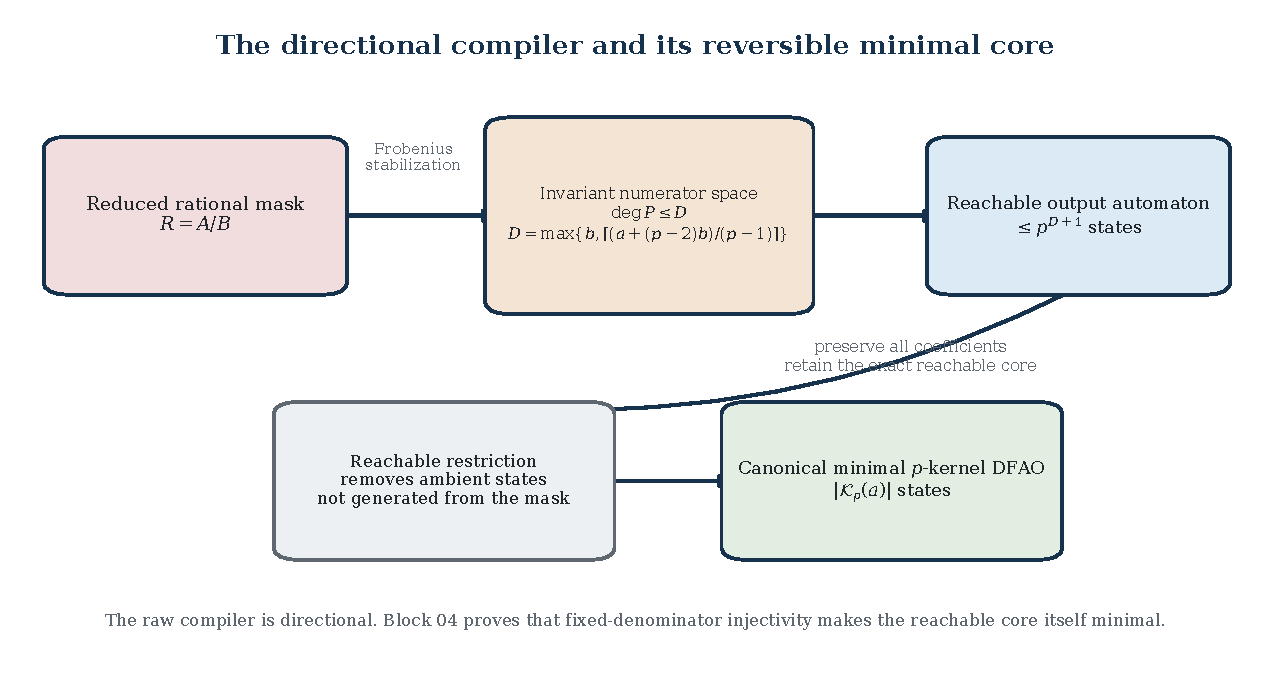
\includegraphics[width=0.99\textwidth]{cartier_compiler_reduction.pdf}
\caption{The raw mask compiler is a directional constructor.  Reachability removes the ambient states outside the numerator orbit.  Injectivity of the fixed-denominator realization then shows that the remaining states are already the unique minimal digital normal form.}
\label{fig:cartier-compiler-reduction}
\end{figure}

\subsection{Triple-overlap and quadruple coherence}

There are four nonempty triple overlaps:
\[
(\Rec,\Rat,\Aut),
\qquad
(\Rec,\Rat,\Mask),
\qquad
(\Rec,\Aut,\Mask),
\qquad
(\Rat,\Aut,\Mask).
\]
All four charts meet on the same unit periodic semantic objects.

\begin{lemma}[Rigidity of normalized fibers]
\label{lem:periodic-fiber-rigidity}
Fix \(a\in\Per_p^{\times,\mathrm{per}}\).  In each of the four normalized charts, the groupoid of presentations of \(a\) is contractible.
\end{lemma}

\begin{proof}
The minimal recurrence with its initial data, the reduced rational function, and the reduced mask are unique, so their fibers are terminal groupoids.  A normalized digital presentation is a reachable minimal automaton.  Any automorphism fixes the start state and commutes with every transition.  Reachability then forces it to fix every state.  Hence its automorphism group is trivial, and any two minimal presentations are joined by the unique behavioral isomorphism.
\end{proof}

\begin{theorem}[Coherence of the periodic heterogeneous atlas]
\label{thm:periodic-atlas-coherence}
Choose every pairwise bridge by the explicit constructions above and choose every comparison \(2\)-cell to be the unique normalized isomorphism over the common sequence.  Then:
\begin{enumerate}[label=\textup{(\roman*)}]
\item every one of the four triple-overlap comparison diagrams commutes;
\item the two composites of comparison cells on the four-chart overlap agree;
\item the quadruple-overlap coherence defect \(\Omega\) is the identity.
\end{enumerate}
\end{theorem}

\begin{proof}
Every comparison in question is an isomorphism between normalized presentations of one fixed semantic sequence.  By \cref{lem:periodic-fiber-rigidity}, there is exactly one such isomorphism.  Any two composites with the same source and target must therefore agree.  This proves all triple laws and the quadruple law simultaneously.
\end{proof}

\begin{figure}[htbp]
\centering
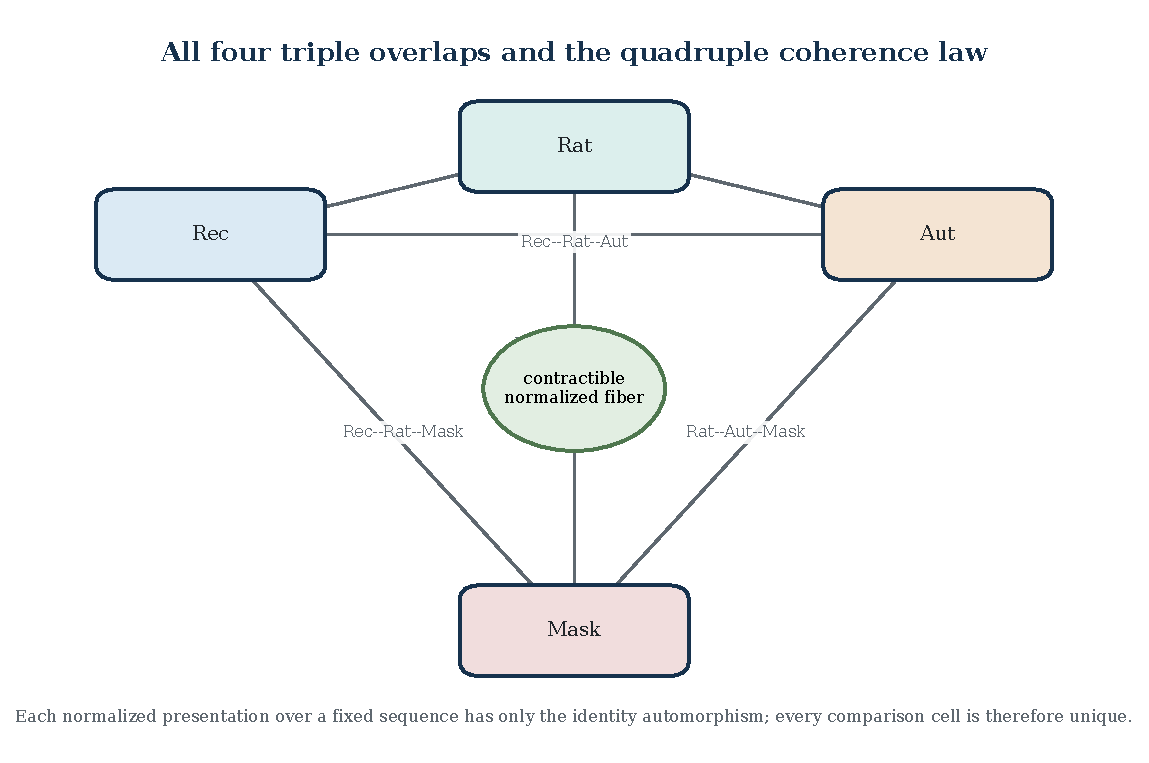
\includegraphics[width=0.86\textwidth]{periodic_coherence_tetrahedron.pdf}
\caption{The coherence tetrahedron.  Contractibility of every normalized semantic fiber makes each comparison cell unique, so all triple and quadruple coherence equations hold automatically after the bridge constructions have been typed.}
\label{fig:periodic-coherence}
\end{figure}

\subsection{Effective descent for objects and morphisms}

Let \(\mathfrak R_p^{\mathrm{per}}\) denote the four-chart pseudofunctor defined by the preceding passports and comparison cells.

\begin{theorem}[First heterogeneous effective-descent theorem]
\label{thm:first-heterogeneous-descent}
The semantic pseudonatural transformation induces an equivalence
\begin{equation}
\label{eq:first-heterogeneous-descent}
\Desc(\mathfrak R_p^{\mathrm{per}})
\simeq
\Per_p^{\times,\mathrm{per}}.
\end{equation}
In particular, descent is effective for both objects and morphisms.
\end{theorem}

\begin{proof}
Given \(a\in\Per_p^{\times,\mathrm{per}}\), form its minimal recurrence, reduced rational OGF, canonical minimal \(p\)-kernel automaton, and reduced rational mask.  The explicit bridges supply a descent object.  This defines a functor
\[
N:\Per_p^{\times,\mathrm{per}}
\longrightarrow
\Desc(\mathfrak R_p^{\mathrm{per}}).
\]
Conversely, any descent object has local presentations whose semantic images agree on every overlap.  Since the semantic target is discrete, they determine one sequence \(a\).  Normalization and \cref{lem:periodic-fiber-rigidity} identify the local presentations with those constructed by \(N(a)\).  Thus \(N\) is essentially surjective and fully faithful.

For morphisms, a compatible local family lies over one equality of semantic sequences.  Each normalized fiber has at most one morphism, so the local family glues uniquely.  Identities, composition, equality, and invertibility are therefore detected componentwise and descend.
\end{proof}

\begin{corollary}[A verified instance of the assembly theorem]
The atlas \(\mathfrak R_p^{\mathrm{per}}\) satisfies realization, semantic adequacy, typed overlaps, higher coherence, effective descent, and preservation for the finite algebraic constructions used in this section.  Therefore \cref{thm:atlas-assembly} applies without a remaining categorical hypothesis on this restricted domain.
\end{corollary}

The conclusion is intentionally local to the selected atlas.  It does not imply effective descent for arbitrary automatic sequences, unrestricted rational masks, general local analytic objects, or the full eight-stratum registry.

\subsection{A compatible complete invariant family}

For \(a\in\Per_p^{\times,\mathrm{per}}\), define the periodic resolved invariant package
\begin{equation}
\label{eq:periodic-invariant-package}
\mathcal J_p(a)
=
\bigl(
T(a),
 w(a),
 m_a(x),
 P_a(z)/Q_a(z),
 \mathcal K_p(a),
 \mathcal A_p(a),
 R_a(z)
\bigr),
\end{equation}
where \(\mathcal A_p(a)\) is the canonical minimal digital automaton.  Its comparison identities include
\begin{equation}
\label{eq:periodic-invariant-identities}
\begin{aligned}
\deg m_a
&=\deg Q_a
=\rank H(a)
=\dim \State_{\min}(a),\\
T(a)
&=\min\{N:m_a\mid x^N-1\}
=\min\{N:Q_a\mid 1-z^N\},\\
|\mathcal A_p(a)|
&=|\mathcal K_p(a)|
\leq T(a)\bigl(\nu_p(T(a))+\operatorname{ord}_{M}(p)\bigr),\\
R_a(z)
&=\frac{F_a(z)}{F_a(z^p)},
\qquad T(a)=p^{\nu_p(T(a))}M,
\quad \gcd(M,p)=1.
\end{aligned}
\end{equation}

\begin{theorem}[Invariant descent and global completeness on the periodic atlas]
\label{thm:periodic-invariant-completeness}
The native invariants in the recurrence, rational, digital, and mask charts admit coherent comparison maps to \(\mathcal J_p\).  These maps descend to
\[
\mathcal J_p:
\Desc(\mathfrak R_p^{\mathrm{per}})
\longrightarrow
\mathbf{Inv}_p^{\mathrm{per}}.
\]
The descended invariant is complete on the declared semantic category.
\end{theorem}

\begin{proof}
Every component of \(\mathcal J_p(a)\) is reconstructed from the coefficient sequence by the explicit normalization procedures above.  Hence every pairwise bridge preserves the package and the comparison cells are identities after semantic identification.  Triple coherence follows from \cref{thm:periodic-atlas-coherence}.  If \(\mathcal J_p(a)=\mathcal J_p(b)\), then the primitive period words agree, so \(a=b\).  Under \cref{eq:first-heterogeneous-descent}, equality of semantic objects is exactly isomorphism in the descent category.
\end{proof}

The completeness claim has a narrow classification target: unit purely periodic sequences over \(\mathbb F_p\).  It is not a complete invariant for all C-finite, all automatic, or all rational functional-Mahler sequences.

\subsection{Exact examples and a normalization boundary}

\begin{table}[htbp]
\centering
\caption{Named exact examples in the heterogeneous periodic atlas.}
\label{tab:block03-examples}
\scriptsize
\begin{tabularx}{\textwidth}{@{}L{0.14\textwidth}L{0.09\textwidth}L{0.11\textwidth}L{0.15\textwidth}L{0.15\textwidth}L{0.09\textwidth}Y@{}}
\toprule
Example & Field / word & Minimal recurrence & Reduced OGF denominator & Reduced mask numerator & Kernel states & \shortstack[l]{Compiler\\bound}\\
\midrule
Even indicator & $\mathbb F_2$ / 10 & $1+x^2$ & $1+z^2$ & $1+z^2$ & 3 & 8\\
Alternating unit & $\mathbb F_3$ / 12 & $1+x$ & $1+z$ & $1+2z+z^2$ & 2 & 9\\
Period-three word & $\mathbb F_2$ / 110 & $1+x+x^2$ & $1+z+z^2$ & $1+z+z^2$ & 3 & 8\\
\bottomrule
\end{tabularx}
\end{table}


\paragraph{Even indicator over \(\mathbb F_2\).}
For the word \(10\),
\[
T=2,
\qquad
m(x)=x^2+1=(x+1)^2,
\qquad
F(z)=\frac{1}{1+z^2},
\qquad
R(z)=1+z^2.
\]
The repeated recurrence root is compatible with pure periodicity because the field has characteristic two.  The canonical \(2\)-kernel has three states: the original sequence, the constant-one sequence, and the constant-zero sequence.  The rational-mask compiler gives the safe ambient bound \(2^3=8\) before reachability restriction.

\paragraph{Alternating unit over \(\mathbb F_3\).}
For the word \(12\),
\[
T=2,
\qquad
m(x)=x+1,
\qquad
F(z)=\frac{1}{1+z},
\qquad
R(z)=\frac{1+z^3}{1+z}=1+2z+z^2.
\]
The recurrence order is one although the minimal period is two.  The \(3\)-kernel consists of the sequence and its negative, giving two minimal digital states.  The compiler bound is nine.

\paragraph{Period-three unit word over \(\mathbb F_2\).}
For the word \(110\),
\[
T=3,
\qquad
m(x)=x^2+x+1,
\qquad
F(z)=\frac{1}{1+z+z^2},
\qquad
R(z)=1+z+z^2.
\]
The reachable pair model has six representatives, while equality of subsequence behavior collapses them to three kernel states.  This is a concrete instance of the directional quotient in \cref{prop:compiler-minimal-core}.

\begin{figure}[htbp]
\centering
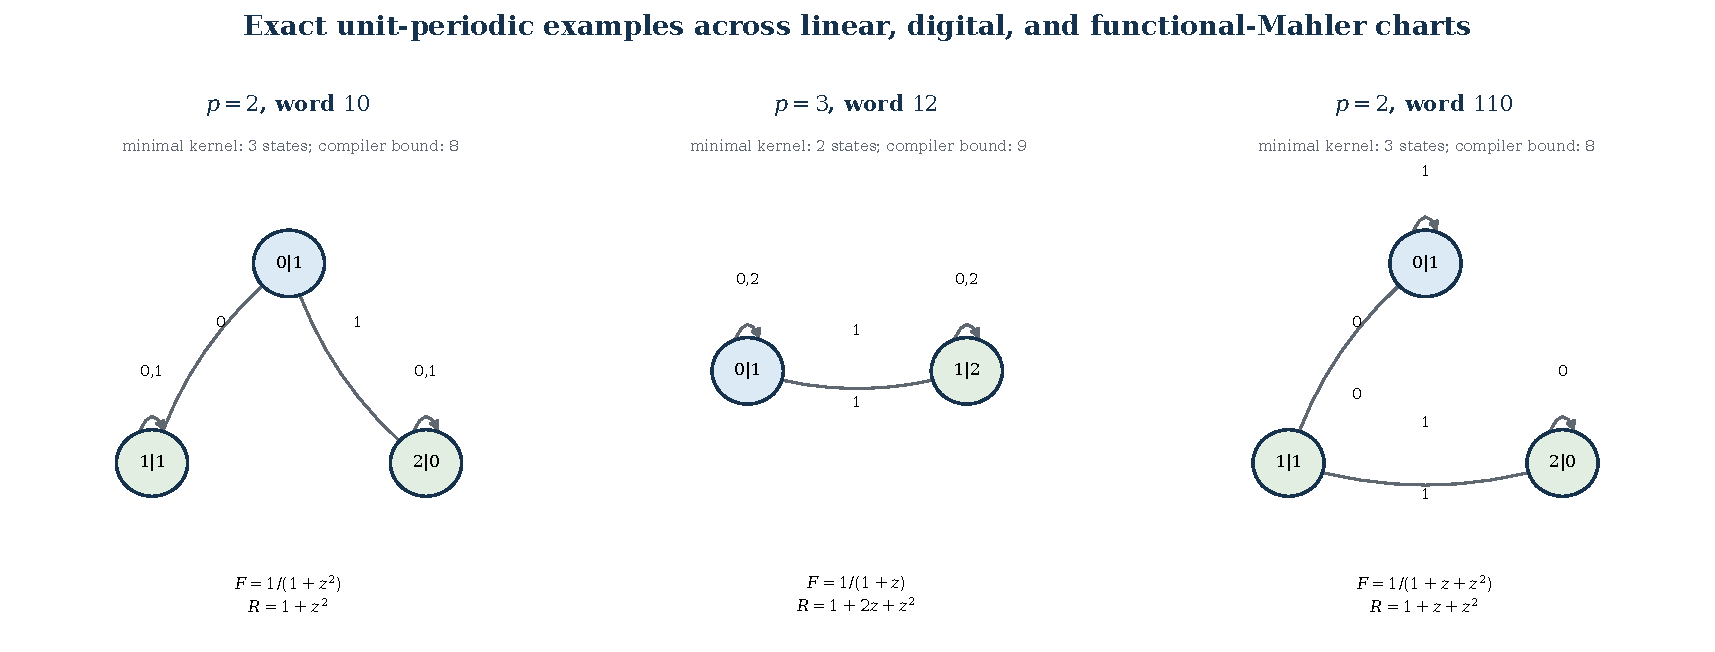
\includegraphics[width=0.99\textwidth]{periodic_example_automata.pdf}
\caption{Three exact examples.  A state label \(s\mid o\) gives the state identifier and output.  The compiler bounds are ambient theorem bounds before reachability restriction, not claims of minimal state count.}
\label{fig:periodic-example-automata}
\end{figure}

\paragraph{Negative control: a nonunit periodic sequence.}
Over \(\mathbb F_2\), the word \(01\) gives
\[
F(z)=\frac{z}{1+z^2}.
\]
Then
\[
\frac{F(z)}{F(z^2)}
=
\frac{1+z^2}{z},
\]
which is Laurent rather than regular at the origin.  The sequence remains purely periodic, C-finite, and automatic, but it is not an object of \(\Mask_2^{\times,\mathrm{per}}\).  This verifies that the unit overlap condition is structural rather than cosmetic.

\subsection{Exact finite verification}

\begin{table}[htbp]
\centering
\caption{Exact finite validation of the Block 03 periodic heterogeneous atlas.}
\label{tab:block03-validation}
\small
\begin{tabularx}{\textwidth}{@{}L{0.28\textwidth}Y@{}}
\toprule
Check & Recorded result\\
\midrule
Enumerated normalized objects & $p=2$ through period 8, $p=3$ through period 6; 583 primitive unit-periodic words.\\
Exact identities and automaton checks & 39805 checks; 0 failures.\\
Arithmetic model & exact prime-field and polynomial arithmetic.\\
Overall status & PASS.\\
Boundary & Finite enumeration validates the declared ranges and implementation formulas. It does not replace the symbolic proofs or establish unrestricted automatic-to-Mahler equivalence.\\
\bottomrule
\end{tabularx}
\end{table}


The supplied verifier enumerates every primitive unit-periodic word over \(\mathbb F_2\) through period eight and over \(\mathbb F_3\) through period six.  For each object it checks, using exact prime-field and polynomial arithmetic:
\begin{enumerate}
\item Berlekamp-Massey recovery of the minimal recurrence;
\item divisibility by \(x^T-1\) and \(1-z^T\);
\item recovery of the least period from both normalized linear charts;
\item the reduced rational functional-Mahler identity;
\item the exact reachable pair model and its behavioral quotient;
\item the multiplier-orbit formula \cref{eq:u-size};
\item coefficient output of the minimal digit automaton;
\item the Cartier compiler state bound \cref{eq:compiler-state-bound-block03}.
\end{enumerate}
The finite computation supports the implementation and examples.  The symbolic theorems above do not depend on the enumeration.

\begin{resultbox}
\textbf{Section result.}
The manuscript now contains a fully declared finite atlas spanning three genuinely different strata: minimal finite-linear recurrences, minimal digital automata, and rational functional-Mahler masks.  Every reversible bridge has a complete passport.  The raw Cartier compiler is retained as a directional constructor with an exact loss statement.  All four triple overlaps and the quadruple coherence equation are proved through rigidity of normalized fibers.  Objects and morphisms descend effectively, and the compatible periodic invariant package is globally complete on the declared unit-periodic semantic category.  This is the first theorem in the manuscript that satisfies the finite heterogeneous completion criterion rather than only the one-stratum cross-presentation criterion.
\end{resultbox}


\section{Rational-mask digital descent beyond pure periodicity}
\label{sec:rational-mask-digital-atlas}

Periodic atlas verified a four-chart atlas on unit purely periodic sequences.  That domain made the linear, rational, digital, and functional-Mahler charts meet simultaneously, but it left open the larger overlap between rational functional-Mahler masks and automatic sequences.  This section removes the periodicity hypothesis while keeping the normalization and bridge standards unchanged.

Fix a prime \(p\).  Let
\[
\RMah_p^{\times}
=
\left\{
F(z)\in 1+z\mathbb F_p[[z]]:
\frac{F(z)}{F(z^p)}\in\mathbb F_p(z)
\right\}
\]
be the discrete category of unit formal series with rational canonical functional-Mahler mask.  This category contains the periodic objects of \cref{sec:periodic-heterogeneous-atlas}, but for odd \(p\) it also contains genuinely nonrational and non-C-finite automatic series.

\subsection{Frobenius-radical characterization}

For a unit formal series, define its canonical local mask by
\begin{equation}
\label{eq:block04-canonical-mask}
R_F(z)
=
\frac{F(z)}{F(z^p)}.
\end{equation}
The coefficientwise infinite product
\begin{equation}
\label{eq:block04-mask-product}
\mathcal M_p[R](z)
=
\prod_{j\geq 0}R\!\left(z^{p^j}\right)
\end{equation}
is well defined for every \(R\in1+z\mathbb F_p[[z]]\), because only finitely many factors contribute to a fixed coefficient.

\begin{theorem}[Frobenius-radical characterization]
\label{thm:frobenius-radical-characterization}
Let \(F\in1+z\mathbb F_p[[z]]\).  Then
\begin{equation}
\label{eq:block04-frobenius-mask}
R_F(z)=F(z)^{1-p}.
\end{equation}
Consequently, the following are equivalent.
\begin{enumerate}[label=\textup{(\roman*)}]
\item The canonical mask \(R_F\) is rational.
\item The power \(F^{p-1}\) belongs to \(\mathbb F_p(z)\).
\item There are coprime polynomials \(A,B\in\mathbb F_p[z]\) with
\[
A(0)=B(0)=1
\]
and
\begin{equation}
\label{eq:block04-rational-mask-equation}
B(z)F(z)=A(z)F(z^p).
\end{equation}
\end{enumerate}
For the reduced mask \(R_F=A/B\), one has
\begin{equation}
\label{eq:block04-radical-equation}
F(z)^{p-1}=\frac{B(z)}{A(z)}.
\end{equation}
The ratio and product constructions are strict inverses:
\[
F\longmapsto R_F,
\qquad
R\longmapsto\mathcal M_p[R].
\]
In particular, every object of \(\RMah_p^{\times}\) is algebraic over \(\mathbb F_p(z)\) of degree at most \(p-1\).
\end{theorem}

\begin{proof}
In characteristic \(p\), Frobenius gives
\[
F(z^p)=F(z)^p.
\]
Substitution into \cref{eq:block04-canonical-mask} gives \cref{eq:block04-frobenius-mask}.  Thus \(R_F\) is rational exactly when \(F^{p-1}=R_F^{-1}\) is rational.  Writing the reduced rational mask as \(A/B\) gives \cref{eq:block04-rational-mask-equation} and \cref{eq:block04-radical-equation}.

Conversely, a reduced rational mask \(A/B\) with unit constant terms defines a unique formal solution of \cref{eq:block04-rational-mask-equation}: the product in \cref{eq:block04-mask-product}.  Telescoping gives
\[
\frac{\mathcal M_p[R](z)}{\mathcal M_p[R](z^p)}=R(z),
\]
while uniqueness follows by comparing coefficients recursively.  Hence the ratio and product constructions are strict inverses.  Finally, \cref{eq:block04-radical-equation} is an algebraic equation of degree \(p-1\).
\end{proof}

\begin{boundary}[Functional Mahler versus Newton-Mahler]
The word ``Mahler'' continues to name two distinct constructions.  This section concerns the functional equation
\[
F(z)=R(z)F(z^p).
\]
It does not identify rational masks with Newton-Mahler expansions
\[
f(x)=\sum_{r\geq0}c_r\binom xr
\]
or with \(p\)-adic analytic interpolation.  Any bridge to that local analytic chart still requires its own passport and proof.
\end{boundary}

\subsection{The rational-collapse obstruction}

Let \(R=A/B\) be reduced and normalized.  For each monic irreducible polynomial \(\pi\in\mathbb F_p[z]\), define
\[
\omega_{\pi}(R)
=
\bigl(v_{\pi}(B)-v_{\pi}(A)\bigr)\bmod(p-1).
\]
Include the valuation at infinity
\[
\omega_{\infty}(R)
=
\bigl(\deg A-\deg B\bigr)\bmod(p-1).
\]
The finite-support family
\begin{equation}
\label{eq:block04-collapse-obstruction}
\omega_{p-1}(R)
=
\bigl(\omega_v(R)\bigr)_v
\end{equation}
is the \emph{rational-collapse obstruction}.

\begin{theorem}[Exact rational-collapse criterion]
\label{thm:rational-collapse-criterion}
Let \(F=\mathcal M_p[A/B]\).  The following are equivalent.
\begin{enumerate}[label=\textup{(\roman*)}]
\item \(F\in\mathbb F_p(z)\).
\item \(B/A\) is a \((p-1)\)-st power in \(\mathbb F_p(z)\).
\item \(\omega_{p-1}(A/B)=0\).
\end{enumerate}
When these conditions hold, there is a unique rational function \(G\in\mathbb F_p(z)\) with \(G(0)=1\) and
\[
G^{p-1}=B/A,
\]
and \(F=G\).

If \(p=2\), every rational mask collapses to a rational series.  If \(p>2\) and \(\omega_{p-1}(A/B)\neq0\), then \(F\) is nonrational, non-C-finite, and not eventually periodic.
\end{theorem}

\begin{proof}
The equivalence of (i) and (ii) follows from \cref{eq:block04-radical-equation}.  If \(B/A=G^{p-1}\), every valuation of \(B/A\) is divisible by \(p-1\), so (ii) implies (iii).

Conversely, suppose all valuation residues vanish.  Since \(A\) and \(B\) are coprime, every irreducible exponent in each polynomial is divisible by \(p-1\).  Factoring into monic irreducibles therefore gives
\[
A=C^{p-1},
\qquad
B=D^{p-1}
\]
for polynomials \(C,D\) after a constant normalization.  The unit conditions \(A(0)=B(0)=1\) remove the remaining scalar obstruction.  Thus \(B/A=(D/C)^{p-1}\).  Multiplying \(D/C\) by its inverse constant term does not change its \((p-1)\)-st power, and gives the unique root with constant term one.  The formal solution is unique, so \(F=G\).

For \(p=2\), the exponent \(p-1\) is one, hence the obstruction group is trivial and \(F=B/A\).  Over a finite field, a rational coefficient series is C-finite and eventually periodic, while an eventually periodic sequence has a rational generating function.  Therefore a nonzero obstruction forces all three failures stated in the theorem.
\end{proof}

\begin{figure}[htbp]
\centering
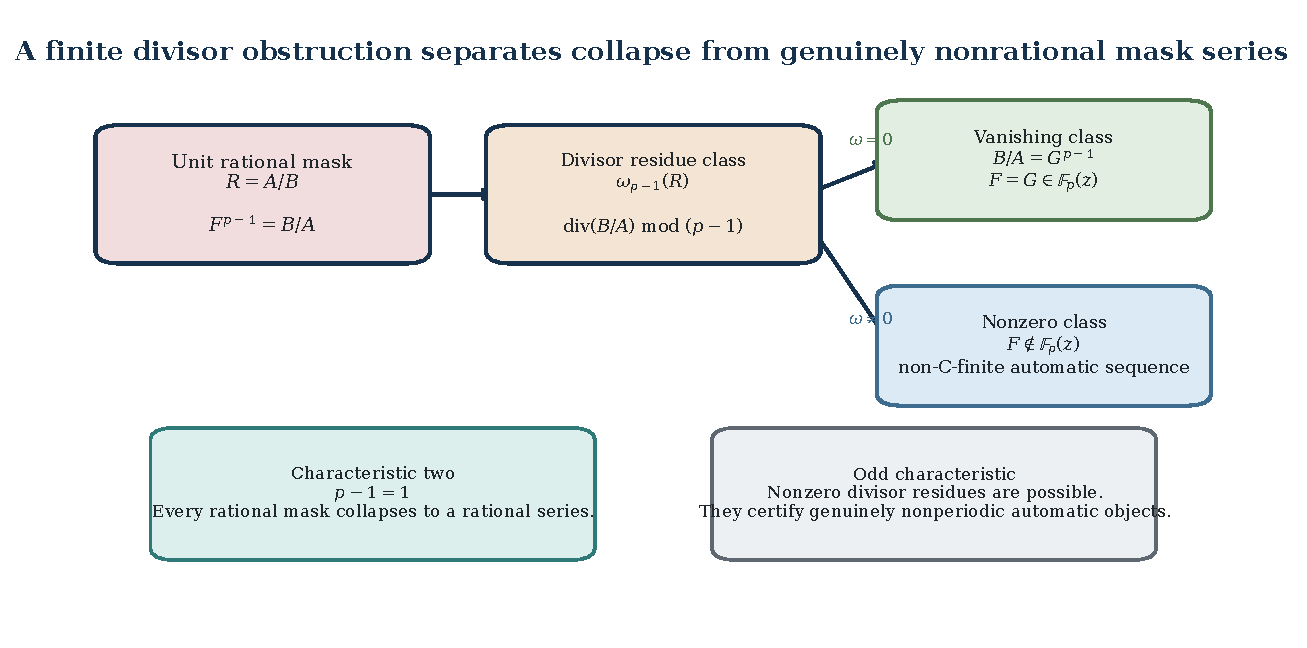
\includegraphics[width=0.98\textwidth]{rational_collapse_obstruction.pdf}
\caption{The rational-collapse obstruction.  A rational mask always gives an automatic series, but it gives a rational or C-finite series exactly on the vanishing divisor-residue locus.}
\label{fig:rational-collapse-obstruction}
\end{figure}

\subsection{Denominator stabilization and the canonical Cartier module}

Write
\[
a=\deg A,
\qquad
b=\deg B,
\qquad
H(z)=A(z)B(z)^{p-2},
\]
and define
\begin{equation}
\label{eq:block04-degree-bound}
D(A,B)
=
\max\left\{
b,
\left\lceil\frac{a+(p-2)b}{p-1}\right\rceil
\right\}.
\end{equation}
Let \(\mathcal P_D=\mathbb F_p[z]_{\leq D}\).  For \(0\leq d<p\), define
\begin{equation}
\label{eq:block04-numerator-transition}
T_d(P)=\Lambda_d(PH),
\end{equation}
where \(\Lambda_d\) selects the coefficients in degrees congruent to \(d\) modulo \(p\).

\begin{theorem}[Fixed-denominator Cartier realization]
\label{thm:fixed-denominator-cartier-realization}
Let \(F=\mathcal M_p[A/B]\) and \(D=D(A,B)\).  Then:
\begin{enumerate}[label=\textup{(\roman*)}]
\item every \(T_d\) preserves \(\mathcal P_D\);
\item the linear map
\begin{equation}
\label{eq:block04-theta-map}
\Theta_{A,B}:\mathcal P_D\longrightarrow\mathbb F_p[[z]],
\qquad
\Theta_{A,B}(P)=\frac{P}{B}F,
\end{equation}
is injective;
\item the transitions intertwine exactly:
\begin{equation}
\label{eq:block04-intertwining}
\Lambda_d\Theta_{A,B}(P)
=
\Theta_{A,B}(T_d(P));
\end{equation}
\item starting from \(P_0=B\), the coefficient of index
\[
n=d_0+d_1p+\cdots+d_{\ell-1}p^{\ell-1}
\]
is
\begin{equation}
\label{eq:block04-compiler-output}
[z^n]F
=
\epsilon_0\!\left(
\Theta_{A,B}
\bigl(T_{d_{\ell-1}}\cdots T_{d_0}B\bigr)
\right),
\end{equation}
where \(\epsilon_0(G)=[z^0]G\).
\end{enumerate}
\end{theorem}

\begin{proof}
If \(\deg P\leq D\), then
\[
\deg(PH)
\leq
D+a+(p-2)b.
\]
Cartier selection divides the retained degrees by \(p\).  The definition of \(D\) gives
\[
\deg T_d(P)
\leq
\left\lfloor\frac{D+a+(p-2)b}{p}\right\rfloor
\leq D.
\]
This proves (i).

The series \(F/B\) is a unit in \(\mathbb F_p[[z]]\).  Multiplication by a unit is injective, so \(\Theta_{A,B}\) is injective.  The rational-mask Cartier identity imported from \cite{FMH} is precisely \cref{eq:block04-intertwining}.  Iterating it from \(\Theta(B)=F\) and taking constant terms proves \cref{eq:block04-compiler-output}.
\end{proof}

For a digit word \(w=d_0\cdots d_{\ell-1}\), read least significant digit first and write
\[
\Lambda_w
=
\Lambda_{d_{\ell-1}}\cdots\Lambda_{d_0}.
\]
Define the Cartier kernel and its linear span by
\begin{equation}
\label{eq:block04-kernel-span}
\mathcal K_p(F)
=
\{\Lambda_wF:w\in\{0,\ldots,p-1\}^{*}\},
\qquad
\mathcal V_p(F)
=
\operatorname{span}_{\mathbb F_p}\mathcal K_p(F).
\end{equation}

\begin{definition}[Canonical Cartier module and Cartier rank]
The canonical Cartier module of \(F\) is
\begin{equation}
\label{eq:block04-cartier-module}
\mathsf C_p(F)
=
\left(
\mathcal V_p(F),
(\Lambda_d|_{\mathcal V_p(F)})_{0\leq d<p},
F,
\epsilon_0
\right).
\end{equation}
Its dimension
\begin{equation}
\label{eq:block04-cartier-rank}
r_p(F)=\dim_{\mathbb F_p}\mathcal V_p(F)
\end{equation}
is the \emph{Cartier rank}.
\end{definition}

\begin{theorem}[Minimality of the canonical Cartier module]
\label{thm:canonical-cartier-minimality}
For every \(F\in\RMah_p^{\times}\), the module \(\mathsf C_p(F)\) is finite dimensional, reachable, and observable.  It is therefore a minimal digit-linear realization of the coefficient function.  Every other reachable-observable digit-linear realization of the same coefficient function is uniquely similar to \(\mathsf C_p(F)\).
\end{theorem}

\begin{proof}
By \cref{thm:fixed-denominator-cartier-realization}, every section \(\Lambda_wF\) lies in the \((D+1)\)-dimensional image of \(\Theta_{A,B}\).  Hence \(\mathcal V_p(F)\) is finite dimensional.  Reachability is built into its definition as the span of the orbit of \(F\).

For observability, let \(G\in\mathcal V_p(F)\) satisfy
\[
\epsilon_0(\Lambda_wG)=0
\]
for every digit word \(w\).  For any \(n\geq0\), choose the base-\(p\) digits of \(n\).  The section identity gives
\[
[z^n]G=\epsilon_0(\Lambda_wG)=0.
\]
Thus \(G=0\), so the observation family separates points.

For uniqueness, let \((V,(L_d),v,\lambda)\) be another reachable-observable realization of the same digit function.  Send the reachable vector \(L_wv\) to \(\Lambda_wF\).  If a linear combination of reachable vectors vanishes, applying every continuation and then \(\lambda\) shows that the corresponding combination of Cartier sections has every coefficient zero.  Observability makes the assignment well defined.  Reachability makes it surjective, and the symmetric construction gives an inverse.  The intertwining, initial-vector, and output identities are immediate.  Any such similarity is determined on the reachable spanning set, so it is unique.
\end{proof}

\subsection{The exact reachable compiler core}

Let \(\mathcal R(A,B)\subseteq\mathcal P_D\) be the finite set of numerator states reachable from \(B\) under the transitions \(T_d\), and let
\[
W(A,B)=\operatorname{span}_{\mathbb F_p}\mathcal R(A,B).
\]

\begin{theorem}[Reachable numerator core]
\label{thm:reachable-numerator-core}
The map \(\Theta_{A,B}\) restricts to
\begin{equation}
\label{eq:block04-reachable-bijections}
\mathcal R(A,B)
\overset{\sim}{\longrightarrow}
\mathcal K_p(F)
\end{equation}
and to a linear isomorphism
\begin{equation}
\label{eq:block04-reachable-span-isomorphism}
W(A,B)
\overset{\sim}{\longrightarrow}
\mathcal V_p(F).
\end{equation}
The reachable deterministic output automaton of the fixed-denominator compiler is already minimal.  No nontrivial output-equivalence quotient remains after reachability restriction.
\end{theorem}

\begin{proof}
For every word \(w\), repeated use of \cref{eq:block04-intertwining} gives
\[
\Theta_{A,B}(T_wB)=\Lambda_wF.
\]
Thus \(\Theta_{A,B}\) maps the reachable numerator set onto the Cartier kernel.  Injectivity of \(\Theta_{A,B}\) makes the map bijective, and taking linear spans gives \cref{eq:block04-reachable-span-isomorphism}.

If two reachable numerators \(P\neq Q\) had identical future output behavior, the two series \(\Theta(P)\) and \(\Theta(Q)\) would have identical coefficients and would therefore be equal.  Injectivity would force \(P=Q\), a contradiction.  Hence all reachable states are behaviorally distinct.  Reachability and distinguishability prove minimality.
\end{proof}

The preceding theorem sharpens the generic reduction language used in Periodic atlas.  A behavioral quotient remains a safe general construction for arbitrary output automata, but it is trivial for the normalized fixed-denominator numerator compiler.

Let
\begin{equation}
\label{eq:block04-kernel-size}
\kappa_p(F)=|\mathcal K_p(F)|.
\end{equation}

\begin{corollary}[Exact state-complexity hierarchy]
\label{cor:cartier-state-hierarchy}
For a reduced rational mask \(A/B\),
\begin{equation}
\label{eq:block04-state-hierarchy}
r_p(F)
\leq
\kappa_p(F)
\leq
p^{r_p(F)}
\leq
p^{D(A,B)+1}.
\end{equation}
Moreover,
\[
r_p(F)=\dim W(A,B),
\qquad
\kappa_p(F)=|\mathcal R(A,B)|.
\]
\end{corollary}

\begin{proof}
The Cartier kernel spans \(\mathcal V_p(F)\), so its cardinality is at least the dimension.  It is a subset of the \(p^{r_p(F)}\) vectors in \(\mathcal V_p(F)\).  Finally, \(\mathcal V_p(F)\) embeds into the \((D+1)\)-dimensional compiler space by \cref{thm:reachable-numerator-core}.
\end{proof}

\begin{figure}[htbp]
\centering
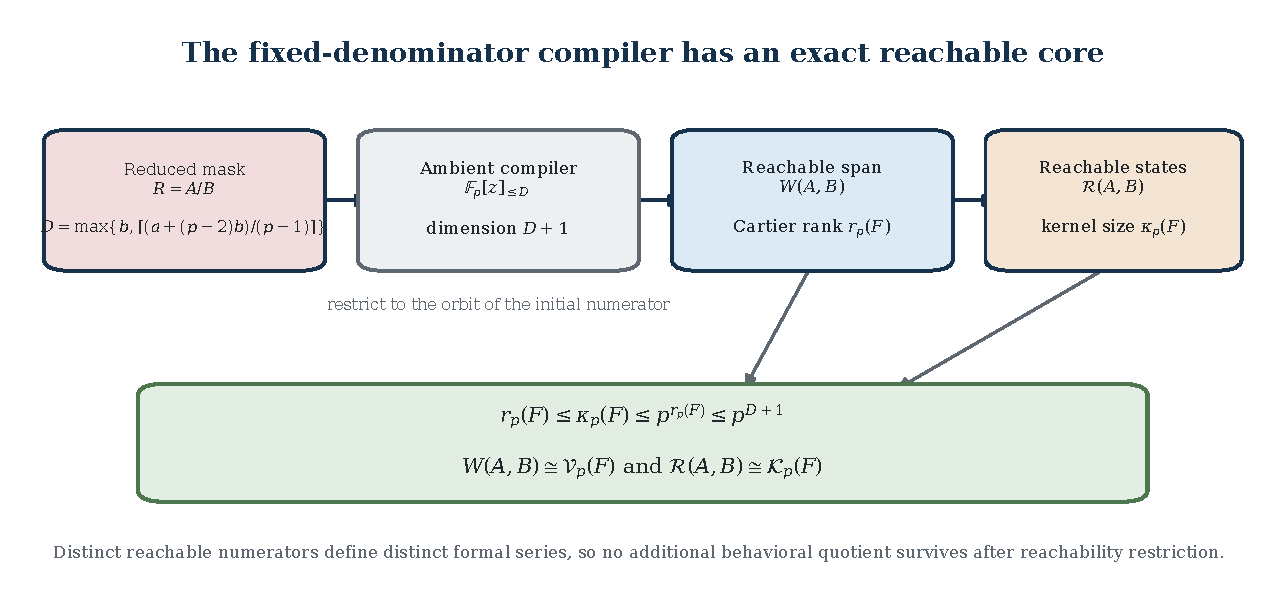
\includegraphics[width=0.99\textwidth]{cartier_state_hierarchy.pdf}
\caption{The exact reachable core of the fixed-denominator compiler.  The linear rank and deterministic state count are different invariants, but both are bounded by the explicit mask degree profile.}
\label{fig:cartier-state-hierarchy}
\end{figure}

\subsection{Three normalized charts}

The rational-mask domain has three normalized charts.

\paragraph{Reduced mask chart.}
An object of \(\Mask_p^{\mathrm{rat}}\) is a reduced rational function
\[
R(z)=\frac{A(z)}{B(z)},
\qquad
A(0)=B(0)=1.
\]
Morphisms preserve the rational function.  The semantics is \(R\mapsto\mathcal M_p[R]\).  The inverse chart map is the canonical ratio \(F\mapsto F/F(z^p)\).

\paragraph{Minimal Cartier-module chart.}
An object of \(\mathbf{Cart}_p^{\mathrm{min,rat}}\) is a finite-dimensional tuple
\[
(V,(L_d)_{d=0}^{p-1},v,\lambda)
\]
that is reachable and observable, whose digit coefficient function belongs to \(\RMah_p^{\times}\).  Morphisms are similarities preserving every \(L_d\), the initial vector, and the output functional.  Its normalized representative is \(\mathsf C_p(F)\).

\paragraph{Minimal digital chart.}
An object of \(\mathbf{Aut}_p^{\mathrm{min,rat}}\) is a reachable minimal least-significant-digit-first \(p\)-DFAO whose coefficient series belongs to \(\RMah_p^{\times}\).  Its canonical representative has state set \(\mathcal K_p(F)\), transition \(G\mapsto\Lambda_dG\), start state \(F\), and output \(G\mapsto G(0)\).

\begin{table}[htbp]
\centering
\caption{Bridge passports for the rational-mask digital atlas.}
\label{tab:block04-bridge-passports}
\small
\begin{tabularx}{\textwidth}{@{}L{0.19\textwidth}L{0.18\textwidth}L{0.16\textwidth}Y@{}}
\toprule
Bridge & Class & Preserved data & Exact boundary\\
\midrule
Mask \(\leftrightarrow\) series & strict inverse pair & every coefficient and the canonical mask & the mask must be rational and unit normalized\\
Series \(\leftrightarrow\) Cartier module & normalized equivalence & all Cartier sections, linear relations, initial vector, output & the module is restricted to reachable-observable realizations\\
Series \(\leftrightarrow\) minimal DFAO & normalized equivalence & the complete \(p\)-kernel and coefficient function & the automaton uses the fixed radix and LSD-first convention\\
Mask \(\to\) ambient compiler & directional constructor & exact coefficients and fixed-denominator transitions & adds unreachable ambient numerator states\\
Ambient compiler \(\to\) normalized core & reachable restriction & all reachable series and all future outputs & discards only states outside the orbit of \(B\)\\
\bottomrule
\end{tabularx}
\end{table}

\begin{theorem}[Rational-mask three-chart equivalence]
\label{thm:rational-mask-three-chart-equivalence}
The semantic functors induce equivalences of groupoids
\begin{equation}
\label{eq:block04-three-chart-equivalence}
\Mask_p^{\mathrm{rat}}
\simeq
\mathbf{Cart}_p^{\mathrm{min,rat}}
\simeq
\mathbf{Aut}_p^{\mathrm{min,rat}}
\simeq
\RMah_p^{\times}.
\end{equation}
The mask-series bridge is a strict inverse pair.  The Cartier and digital bridges are normalized equivalences with unique comparison isomorphisms.
\end{theorem}

\begin{proof}
The strict mask-series equivalence is \cref{thm:frobenius-radical-characterization}.  The canonical Cartier construction gives an object of the second chart, and \cref{thm:canonical-cartier-minimality} gives a unique similarity from every other minimal realization of the same series.  The canonical \(p\)-kernel automaton is finite by \cref{thm:fixed-denominator-cartier-realization}.  It is reachable by construction.  Distinct kernel series differ in some coefficient, and the digit word for that coefficient distinguishes their future outputs, so the automaton is minimal.  The usual behavioral map gives the unique isomorphism from any other reachable minimal DFAO for the same series.
\end{proof}

\begin{figure}[htbp]
\centering
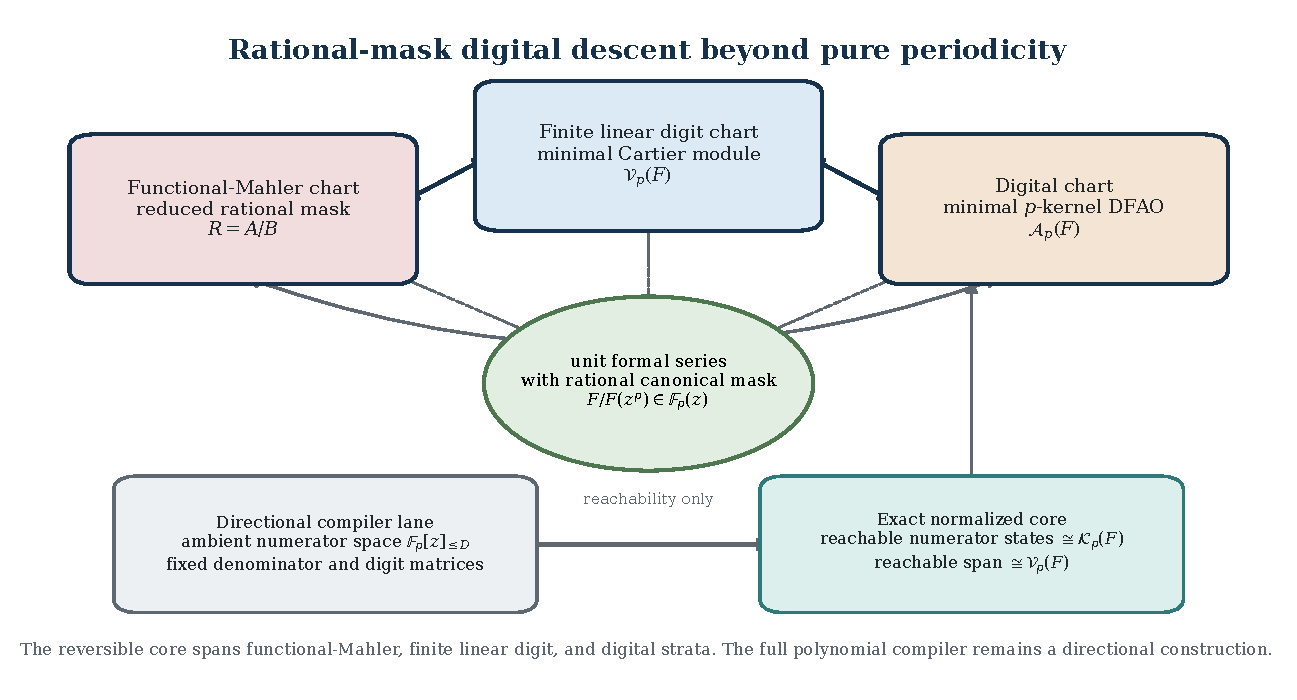
\includegraphics[width=0.98\textwidth]{rational_mask_digital_atlas.pdf}
\caption{The Rational-mask atlas atlas.  The normalized reversible core contains a rational mask, a minimal Cartier module, and a minimal digital automaton.  The full polynomial compiler remains a larger directional presentation.}
\label{fig:rational-mask-digital-atlas}
\end{figure}

\subsection{Coherence and effective descent}

\begin{lemma}[Rigidity of rational-mask normalized fibers]
\label{lem:rational-mask-fiber-rigidity}
Fix \(F\in\RMah_p^{\times}\).  The groupoid of normalized presentations of \(F\) in each of the three charts is contractible.
\end{lemma}

\begin{proof}
The reduced canonical mask is unique.  Any automorphism of a reachable Cartier module that fixes the initial vector and commutes with all digit operators fixes a spanning set, hence is the identity.  Any automorphism of a reachable deterministic automaton that fixes the start state and commutes with every digit transition fixes every state, hence is the identity.  Existence and uniqueness of isomorphisms between two normalized realizations follow from \cref{thm:canonical-cartier-minimality,thm:rational-mask-three-chart-equivalence}.
\end{proof}

Let \(\mathfrak R_p^{\mathrm{rm}}\) denote the three-chart pseudofunctor defined by the passports above.

\begin{theorem}[Rational-mask coherence and effective descent]
\label{thm:rational-mask-effective-descent}
Choose every pairwise bridge by the canonical constructions and every comparison cell by the unique normalized isomorphism over the common series.  Then the triple-overlap coherence law holds, and
\begin{equation}
\label{eq:block04-effective-descent}
\Desc(\mathfrak R_p^{\mathrm{rm}})
\simeq
\RMah_p^{\times}.
\end{equation}
Descent is effective for objects and morphisms.
\end{theorem}

\begin{proof}
On the only nonempty triple overlap, both composites are isomorphisms between normalized presentations of the same series.  By \cref{lem:rational-mask-fiber-rigidity}, the isomorphism is unique, so the comparison diagram commutes.

Given \(F\in\RMah_p^{\times}\), its reduced mask, canonical Cartier module, and minimal \(p\)-kernel automaton form descent data.  Conversely, compatible local objects have one common semantic series.  Fiber rigidity identifies them uniquely with its normalized presentations.  The same argument applies to morphisms.  Hence the normalization functor is fully faithful and essentially surjective.
\end{proof}

This theorem is strictly broader than \cref{thm:first-heterogeneous-descent}: no periodicity or C-finiteness hypothesis is imposed.  It is also strictly narrower than an atlas of all automatic sequences, because an automatic series may have a nonrational canonical mask.

\subsection{Compatible invariants and collapse stratification}

For \(F\in\RMah_p^{\times}\), define
\begin{equation}
\label{eq:block04-invariant-package}
\mathcal J_p^{\mathrm{rm}}(F)
=
\left(
R_F,
\omega_{p-1}(R_F),
D(R_F),
\mathcal V_p(F),
r_p(F),
\mathcal K_p(F),
\kappa_p(F),
\mathcal A_p(F)
\right).
\end{equation}

\begin{theorem}[Invariant descent on the rational-mask atlas]
\label{thm:rational-mask-invariant-descent}
The native mask, Cartier-module, and automaton invariants admit coherent comparison maps to \(\mathcal J_p^{\mathrm{rm}}\).  They descend to the category in \cref{eq:block04-effective-descent}.  The descended invariant is complete on \(\RMah_p^{\times}\).
\end{theorem}

\begin{proof}
The fixed-denominator intertwining theorem identifies the reachable numerator span with \(\mathcal V_p(F)\) and the reachable numerator set with \(\mathcal K_p(F)\).  Hence all components of the package agree under the bridges.  Coherence follows from \cref{thm:rational-mask-effective-descent}.  If two packages agree, their reduced canonical masks agree.  The coefficientwise mask product then reconstructs the same formal series, so the semantic objects are equal.
\end{proof}

The obstruction \(\omega_{p-1}\) divides the semantic category into two exact loci:
\[
\RMah_p^{\times}
=
\RMah_{p,\mathrm{col}}^{\times}
\sqcup
\RMah_{p,\mathrm{ncol}}^{\times}.
\]
The collapse locus consists of rational, hence ultimately periodic, series.  The noncollapse locus consists of non-C-finite automatic series.  The unit-periodic atlas of Periodic atlas is the persistent, zero-transient subatlas inside \(\RMah_{p,\mathrm{col}}^{\times}\).

\subsection{Exact examples and strict boundaries}

\begin{table}[htbp]
\centering
\caption{Named exact examples in the rational-mask digital atlas.}
\label{tab:block04-examples}
\scriptsize
\begin{tabularx}{\textwidth}{@{}L{0.18\textwidth}L{0.07\textwidth}L{0.17\textwidth}L{0.20\textwidth}L{0.09\textwidth}Y@{}}
\toprule
Example & Field & Reduced mask $A/B$ & First coefficients & $r_p/\kappa_p$ & \shortstack[l]{Collapse status /\\compiler bound}\\
\midrule
Cantor-digit indicator & $\mathbb F_3$ & $(1+z)/(1)$ & \texttt{\seqsplit{110110000110110000}} & $1/2$ & \shortstack[l]{non-collapse\\compiler\\bound $9$}\\
Square-root denominator & $\mathbb F_3$ & $(1)/(1+z)$ & \texttt{\seqsplit{121121000121121000}} & $2/4$ & \shortstack[l]{non-collapse\\compiler\\bound $9$}\\
Alternating collapse & $\mathbb F_3$ & $(1+2z+z^2)/(1)$ & \texttt{\seqsplit{121212121212121212}} & $1/2$ & \shortstack[l]{collapse\\compiler\\bound $9$}\\
Finite transient & $\mathbb F_2$ & $(1)/(1+z+z^2)$ & \texttt{\seqsplit{111000000000000000}} & $3/4$ & \shortstack[l]{collapse\\compiler\\bound $8$}\\
\bottomrule
\end{tabularx}
\end{table}


\paragraph{Cantor-digit indicator.}
Over \(\mathbb F_3\), let
\[
R(z)=1+z.
\]
Then
\[
F(z)=\prod_{j\geq0}(1+z^{3^j})
\]
has coefficient one exactly when the ternary expansion of the index uses only the digits zero and one.  The functional equation is
\[
F(z)=(1+z)F(z^3),
\qquad
F(z)^2=\frac1{1+z}.
\]
The factor \(1+z\) has odd divisor multiplicity, so the collapse obstruction is nonzero.  Thus the sequence is automatic but not C-finite or eventually periodic.  The canonical automaton has two states, while the Cartier rank is one.

\paragraph{A genuine denominator example.}
Over \(\mathbb F_3\), take
\[
R(z)=\frac1{1+z}.
\]
Then
\[
F(z)^2=1+z.
\]
The reduced denominator remains fixed under every Cartier section.  The ambient compiler has dimension two, its reachable numerator set is
\[
\{0,1,2,1+z\},
\]
and its reachable span has dimension two.  Hence
\[
r_3(F)=2,
\qquad
\kappa_3(F)=4.
\]
The nonzero collapse obstruction again proves that the automatic coefficient sequence is not eventually periodic.

\paragraph{Collapse back to the periodic atlas.}
For
\[
R(z)=(1+z)^2=1+2z+z^2
\]
over \(\mathbb F_3\), one has
\[
F(z)^2=\frac1{(1+z)^2},
\qquad
F(z)=\frac1{1+z}.
\]
The coefficients alternate between one and two.  This object lies in the rational-collapse locus and in the unit-periodic atlas of Periodic atlas.

\paragraph{Characteristic-two transient.}
Over \(\mathbb F_2\), choose
\[
R(z)=\frac1{1+z+z^2}.
\]
Since \(p-1=1\),
\[
F(z)=1+z+z^2.
\]
Its coefficient sequence is \(1,1,1,0,0,\ldots\).  It is ultimately periodic but not purely periodic.  This is the simplest exact witness that Rational-mask atlas extends the semantic domain even in characteristic two.

\begin{figure}[htbp]
\centering
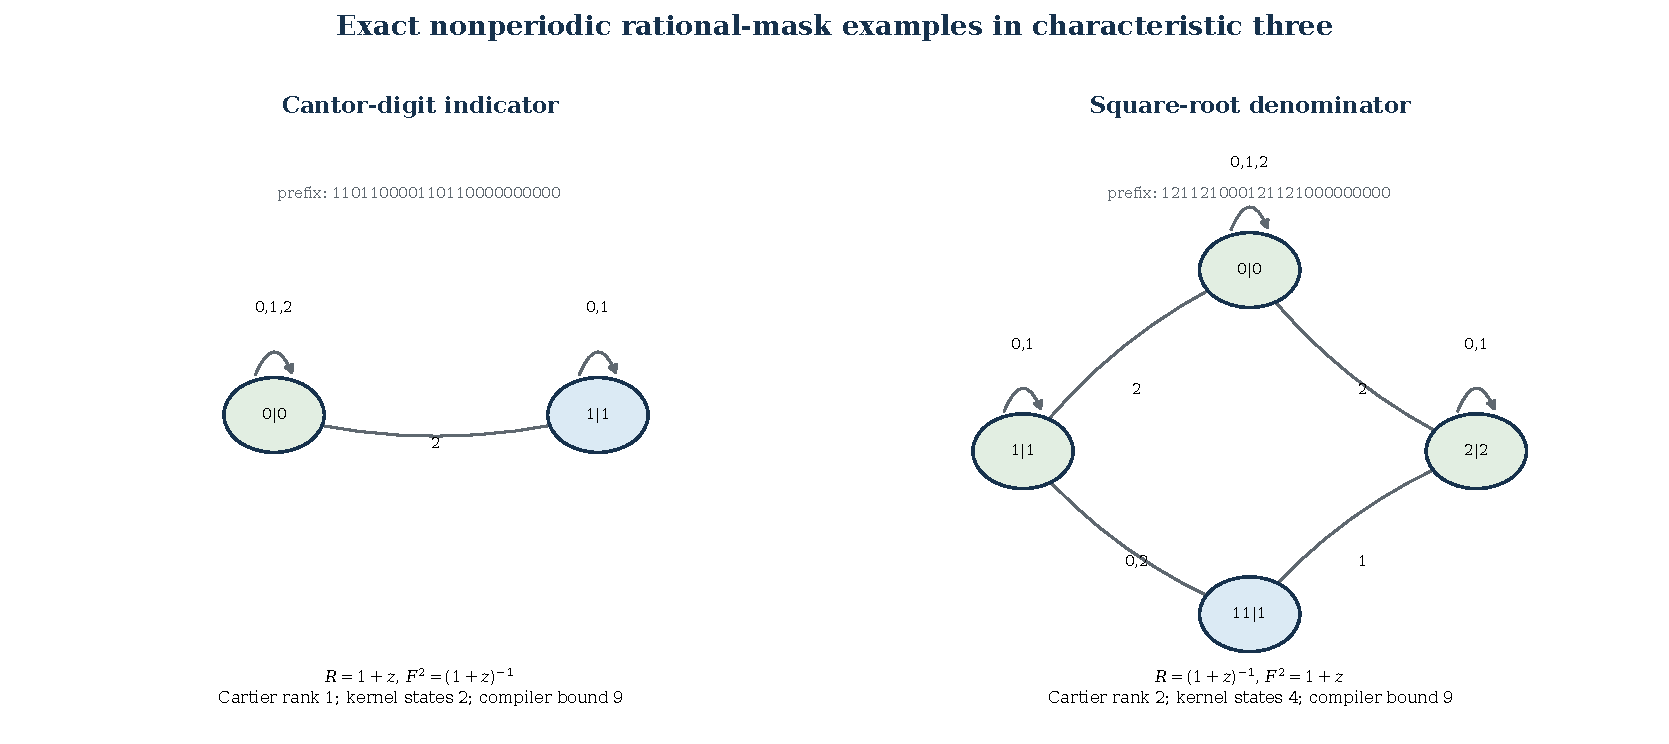
\includegraphics[width=0.99\textwidth]{rational_mask_nonperiodic_examples.pdf}
\caption{Two exact nonperiodic objects in the rational-mask atlas.  State labels give the reachable numerator polynomial followed by its output.}
\label{fig:rational-mask-nonperiodic-examples}
\end{figure}

\paragraph{Negative control: automatic does not imply rational mask.}
Let \(t_n\in\mathbb F_2\) be the parity of the binary digit sum of \(n\), and put
\[
u_n=1+t_n.
\]
The sequence \(u\) is unit and \(2\)-automatic.  It is not eventually periodic.  Indeed, eventual period \(T\) would propagate backwards through the identities
\[
t_{2^k+n}=1+t_n
\qquad
(0\leq n<2^k)
\]
and force a pure period \(T\).  Writing \(T=2^{\nu}q\) with \(q\) odd, the binary digit count of \(2^m-T\) has parity
\[
m-\nu-s_2(q-1)
\]
for all sufficiently large \(m\).  Choosing the parity of \(m\) makes
\[
t_{2^m-T}\neq t_{2^m},
\]
contradicting pure periodicity.

Let \(U(z)=\sum_{n\geq0}u_nz^n\).  If its canonical mask were rational, then \cref{thm:rational-collapse-criterion} with \(p=2\) would make \(U\) rational, hence eventually periodic.  Therefore \(U/U(z^2)\) is not rational.  The rational-mask atlas is a proper normalized subatlas of the unit automatic stratum.

\subsection{Exact finite verification}

\begin{table}[htbp]
\centering
\caption{Exact finite validation of the Block 04 rational-mask digital atlas.}
\label{tab:block04-validation}
\small
\begin{tabularx}{\textwidth}{@{}L{0.28\textwidth}Y@{}}
\toprule
Check & Recorded result\\
\midrule
Enumerated reduced unit masks & $p=2$ with $\deg A,\deg B\leq 3$, $p=3$ with $\deg A,\deg B\leq 2$, $p=5$ with $\deg A,\deg B\leq 1$; 125 masks in total.\\
Rational-collapse split & 51 collapse masks and 74 genuinely nonrational mask series.\\
Exact identities and state checks & 11391 checks; 0 failures.\\
Arithmetic model & exact polynomial, finite-field, Cartier-transition, and formal-series arithmetic.\\
Overall status & PASS.\\
Boundary & Finite enumeration checks the compiler, reachable Cartier module, state hierarchy, examples, and collapse classification on the declared ranges. It does not replace the unbounded proofs or classify all automatic sequences.\\
\bottomrule
\end{tabularx}
\end{table}


The Rational-mask atlas verifier enumerates every reduced unit mask with
\[
\deg A,\deg B\leq3\quad(p=2),
\qquad
\deg A,\deg B\leq2\quad(p=3),
\qquad
\deg A,\deg B\leq1\quad(p=5).
\]
For every mask it checks, using exact finite-field and polynomial arithmetic:
\begin{enumerate}
\item the invariant degree bound on the full ambient numerator space;
\item the functional-equation coefficient recursion against compiler output;
\item transition closure and fixed-denominator intertwining;
\item distinguishability of every pair of reachable numerator states;
\item the identities
\[
W(A,B)\cong\mathcal V_p(F),
\qquad
\mathcal R(A,B)\cong\mathcal K_p(F);
\]
\item the state hierarchy in \cref{eq:block04-state-hierarchy};
\item characteristic-two collapse and the named collapse or noncollapse examples.
\end{enumerate}
The finite calculation validates the implementation on the recorded ranges.  It is not used as a substitute for the unbounded proofs.

\begin{resultbox}
\textbf{Section result.}
The verified heterogeneous atlas now extends beyond pure periodicity.  Every unit rational functional-Mahler mask over \(\mathbb F_p\) has a finite canonical Cartier module and a finite canonical \(p\)-kernel automaton.  The three normalized charts satisfy coherence and effective descent.  The fixed-denominator compiler has an exact reachable core: reachable numerator states are already the minimal digital states, and their span is the minimal Cartier module.  The rational-collapse obstruction separates the ultimately periodic sublocus from genuinely non-C-finite automatic series.  The resulting invariant package is globally complete on the declared rational-mask semantic category, but no claim is made for automatic sequences whose canonical mask is nonrational.
\end{resultbox}

\section{Fixed-radix regular normalization and the automatic finite-orbit boundary}
\label{sec:block05-regular}

Rational-mask atlas closes a substantial automatic slice, but its semantic domain is still defined by the existence of a rational functional-Mahler mask.  The next digital question is more basic and more general: what is the canonical normalized representation of a sequence whose complete fixed-radix section orbit spans a finite-dimensional vector space, even when that orbit itself is infinite?

This section answers that question over a field.  It separates two invariants that coincide only in special cases:
\[
\text{linear section rank}
\qquad\text{and}\qquad
\text{cardinality of the section orbit}.
\]
The first controls regularity and minimal digit-linear dimension.  The second controls automaticity and minimal deterministic-state cardinality.  Their exact relationship is the automatic--regular boundary developed below.

\begin{figure}[htbp]
\centering
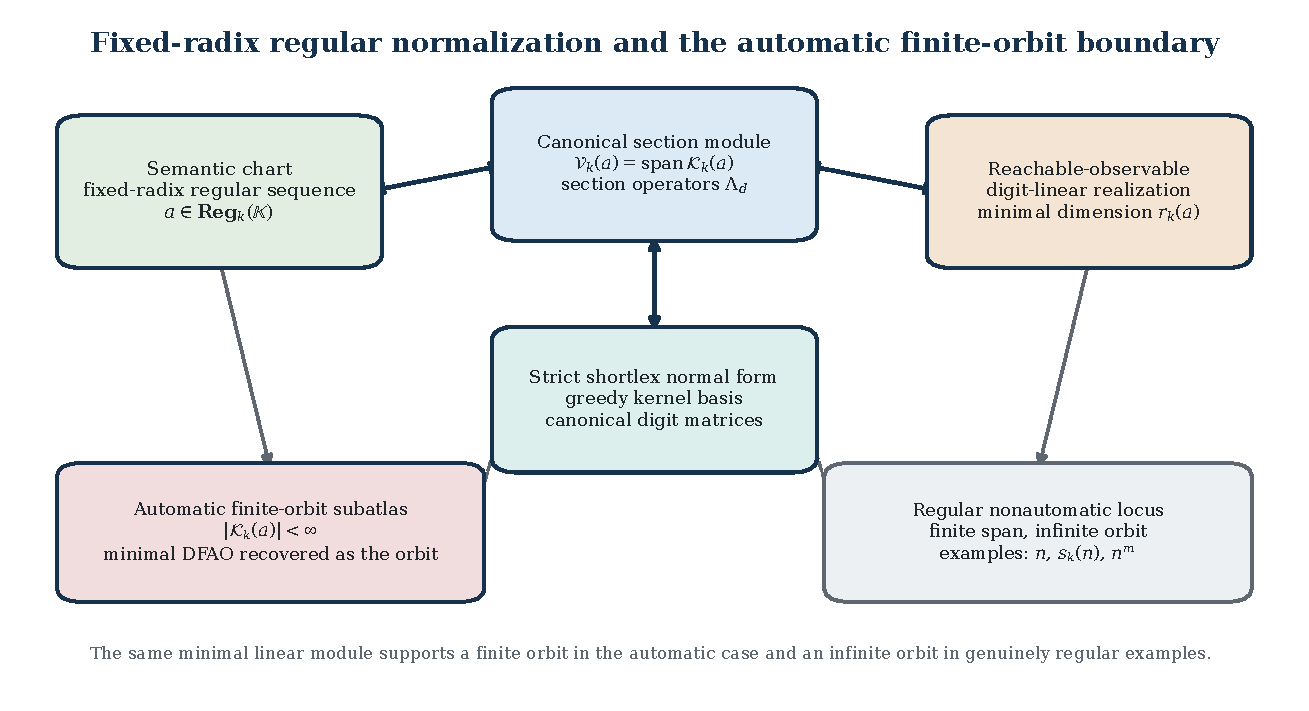
\includegraphics[width=0.99\textwidth]{regular_fixed_radix_atlas.pdf}
\caption{The fixed-radix regular atlas.  The canonical section module and its strict shortlex matrix form exist throughout the regular locus.  The minimal DFAO chart appears exactly on the finite-orbit sublocus.}
\label{fig:regular-fixed-radix-atlas}
\end{figure}

\subsection{Section operators and the canonical kernel module}

Fix an integer radix \(k\geq2\) and a field \(K\).  Let
\[
\Sigma_k=\{0,1,\ldots,k-1\}.
\]
Words are read from least significant digit to most significant digit.  For
\[
w=d_0d_1\cdots d_{\ell-1}\in\Sigma_k^*,
\]
define
\[
|w|=\ell,
\qquad
[w]_k=\sum_{j=0}^{\ell-1}d_jk^j.
\]
The empty word \(\varepsilon\) has length zero and value zero.

For a sequence \(a=(a_n)_{n\geq0}\in K^{\mathbb N}\), define the digit-section operators
\[
(\Lambda_d a)(n)=a(kn+d),
\qquad 0\leq d<k.
\]
For a word \(w=d_0\cdots d_{\ell-1}\), put
\[
\Lambda_w
=
\Lambda_{d_{\ell-1}}\cdots\Lambda_{d_1}\Lambda_{d_0}.
\]
Then
\begin{equation}
(\Lambda_w a)(n)
=
 a\bigl(k^{|w|}n+[w]_k\bigr).
\label{eq:block05-word-section}
\end{equation}

\begin{definition}[Fixed-radix kernel and section module]
The \(k\)-kernel and its linear span are
\[
\mathcal K_k(a)
=
\{\Lambda_w a:w\in\Sigma_k^*\},
\qquad
\mathcal V_k(a)
=
\Span_K\mathcal K_k(a).
\]
The sequence is \emph{\(k\)-regular over \(K\)} when \(\mathcal V_k(a)\) is finite dimensional.  Its regular rank is
\[
r_k(a)=\dim_K\mathcal V_k(a).
\]
It is \emph{\(k\)-automatic in the present reading convention} when \(\mathcal K_k(a)\) is finite.  In that case set
\[
\kappa_k(a)=|\mathcal K_k(a)|.
\]
\end{definition}

The terminology records two different finiteness statements.  Regularity asks for a finite-dimensional linear hull.  Automaticity asks for a finite orbit under the section semigroup itself.

\begin{definition}[Digit-linear realization]
A digit-linear realization of \(a\) is a tuple
\[
\mathsf L=(W,A_0,\ldots,A_{k-1},v,\lambda),
\]
where \(W\) is a finite-dimensional \(K\)-vector space, \(A_d\in\End_K(W)\), \(v\in W\), and \(\lambda\in W^*\), such that for every word \(w=d_0\cdots d_{\ell-1}\),
\begin{equation}
a_{[w]_k}
=
\lambda A_wv,
\qquad
A_w=A_{d_{\ell-1}}\cdots A_{d_0}.
\label{eq:block05-digit-linear-semantics}
\end{equation}
Because different words can represent the same integer after terminal high zeros are appended, equation \eqref{eq:block05-digit-linear-semantics} includes the required leading-zero consistency.
\end{definition}

\begin{theorem}[Section-module realization theorem]
\label{thm:block05-section-module-realization}
For a sequence \(a\in K^{\mathbb N}\), the following are equivalent:
\begin{enumerate}
\item \(a\) is \(k\)-regular over \(K\);
\item \(a\) admits a finite-dimensional digit-linear realization.
\end{enumerate}
When these conditions hold, the tuple
\begin{equation}
\mathsf C_k(a)
=
\bigl(
\mathcal V_k(a),
\Lambda_0,\ldots,\Lambda_{k-1},
 a,
\epsilon_0
\bigr),
\qquad
\epsilon_0(f)=f(0),
\label{eq:block05-canonical-section-module}
\end{equation}
is a canonical realization of dimension \(r_k(a)\).
\end{theorem}

\begin{proof}
Assume first that \(\mathcal V_k(a)\) is finite dimensional.  It is invariant under every \(\Lambda_d\) by construction.  Choose any basis, represent the section operators by matrices, take the initial vector to be \(a\), and take output to be evaluation at zero.  For every word \(w\),
\[
\epsilon_0(\Lambda_wa)
=(\Lambda_wa)(0)
=a_{[w]_k},
\]
so the resulting realization satisfies \eqref{eq:block05-digit-linear-semantics}.

Conversely, suppose \(a\) has a realization \((W,A_d,v,\lambda)\).  For \(x\in W\), define its represented behavior by
\[
\mathcal B(x)(n)
=
\lambda A_{\operatorname{dig}_k(n)}x,
\]
where \(A_{\operatorname{dig}_k(n)}\) is the product associated with the canonical least-significant-digit-first expansion of \(n\).  Equation \eqref{eq:block05-digit-linear-semantics} and concatenation of digit words give
\[
\Lambda_w a
=
\mathcal B(A_wv).
\]
Hence every kernel section belongs to \(\mathcal B(W)\), so
\[
\dim_K\mathcal V_k(a)
\leq
\dim_K W.
\]
Thus \(a\) is regular.  The realization in \eqref{eq:block05-canonical-section-module} has dimension exactly \(r_k(a)\).
\end{proof}

\begin{proposition}[Reachability and observability]
\label{prop:block05-reach-observe}
The canonical section realization \(\mathsf C_k(a)\) is linearly reachable and observable:
\[
\Span_K\{\Lambda_wa:w\in\Sigma_k^*\}
=
\mathcal V_k(a),
\]
and
\[
\bigcap_{w\in\Sigma_k^*}
\ker(\epsilon_0\Lambda_w)
=
\{0\}.
\]
\end{proposition}

\begin{proof}
Reachability is the definition of \(\mathcal V_k(a)\).  If \(f\in\mathcal V_k(a)\) satisfies \((\epsilon_0\Lambda_w)(f)=0\) for every word \(w\), then
\[
f([w]_k)=0
\]
for every word.  Every nonnegative integer has such an expansion, so \(f=0\).
\end{proof}

\subsection{Word-Hankel rank and minimal digit-linear dimension}

The canonical module can be read directly from a Hankel-type matrix indexed by digit words.

\begin{definition}[Word-Hankel matrix]
The fixed-radix word-Hankel matrix of \(a\) is the infinite matrix
\begin{equation}
H_a(u,v)
=
 a_{[u]_k+k^{|u|}[v]_k}
=
(\Lambda_u a)([v]_k),
\qquad
u,v\in\Sigma_k^*.
\label{eq:block05-word-hankel}
\end{equation}
\end{definition}

\begin{theorem}[Regular rank theorem]
\label{thm:block05-regular-rank}
Let \(a\) be \(k\)-regular over \(K\).  Then
\begin{equation}
\boxed{
 r_k(a)
 =
 \rank_K H_a
 =
 \min\{\dim_K W:W\text{ supports a digit-linear realization of }a\}.
}
\label{eq:block05-rank-identity}
\end{equation}
Moreover:
\begin{enumerate}
\item there exist finite word sets \(U,V\subset\Sigma_k^*\), each of cardinality \(r_k(a)\), for which the minor \(H_a[U,V]\) is nonsingular;
\item every reachable-observable realization of dimension \(r_k(a)\) is isomorphic to \(\mathsf C_k(a)\);
\item any two minimal reachable-observable realizations are related by a unique similarity intertwining all digit operators, the initial vector, and the output functional.
\end{enumerate}
\end{theorem}

\begin{proof}
The row indexed by \(u\) in \(H_a\) is the behavior of the section \(\Lambda_u a\) evaluated on all continuation words.  By observability in \cref{prop:block05-reach-observe}, evaluation on all words is injective on \(\mathcal V_k(a)\).  Therefore the row span of \(H_a\) is naturally isomorphic to \(\mathcal V_k(a)\), and
\[
\rank_K H_a=r_k(a).
\]

For an arbitrary realization \((W,A_d,v_{\mathrm{in}},\lambda)\), concatenation gives the factorization
\[
H_a(u,v)
=
\lambda A_vA_uv_{\mathrm{in}}.
\]
Thus \(H_a\) factors through \(W\), so \(\rank H_a\leq\dim W\).  The canonical realization has dimension \(r_k(a)\), proving the minimality formula.

An infinite matrix of finite rank \(r_k(a)\) has a nonsingular finite \(r_k(a)\times r_k(a)\) minor, which gives the first assertion.  For the remaining assertions, define the behavior map of any realization by
\[
\mathcal B_W(x)(n)=\lambda A_{\operatorname{dig}_k(n)}x.
\]
Observability makes this map injective.  Reachability and equality of the represented sequence make its image equal to \(\mathcal V_k(a)\).  In minimal dimension it is therefore an isomorphism intertwining the digit operators, initial vector, and output.  Composing the two behavior isomorphisms gives the unique similarity between any two minimal reachable-observable realizations.
\end{proof}

\begin{figure}[htbp]
\centering
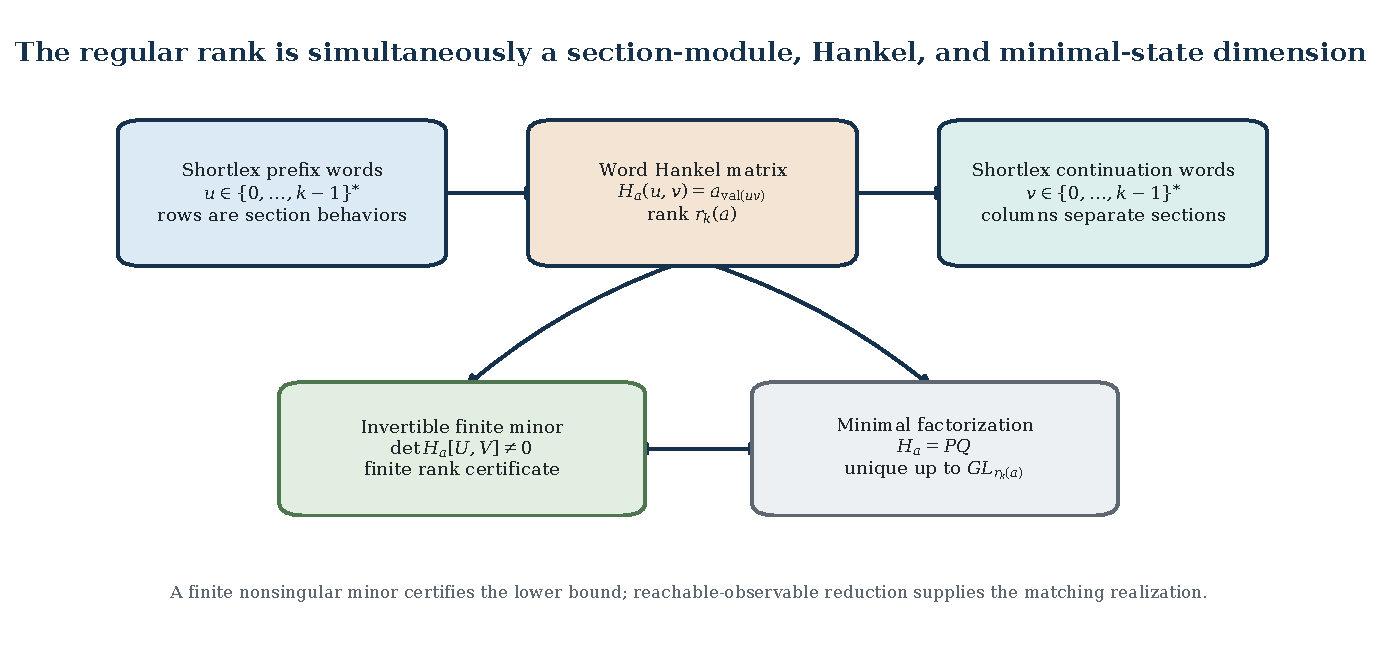
\includegraphics[width=0.99\textwidth]{regular_hankel_rank.pdf}
\caption{Three exact meanings of the regular rank.  The finite nonsingular minor is a certificate rather than an approximation: it proves a lower bound that is attained by the canonical section module.}
\label{fig:regular-hankel-rank}
\end{figure}

\begin{remark}[Finite certification]
The theorem is infinite in statement but finite in certificate.  A proposed rank \(r\) can be certified by:
\begin{enumerate}
\item an explicit \(r\)-dimensional section-stable span containing \(a\), which proves \(r_k(a)\leq r\);
\item an explicit nonsingular \(r\times r\) word-Hankel minor, which proves \(r_k(a)\geq r\).
\end{enumerate}
When both are supplied, the regular rank is exact.
\end{remark}

\subsection{Strict shortlex normalization}

Minimal realizations are unique up to similarity, but the stratified atlas needs a literal normalized chart rather than an unnamed similarity class.  The actual section functions supply a canonical basis choice.

Order \(\Sigma_k^*\) by shortlex order: shorter words precede longer words, and words of equal length are ordered lexicographically.  Starting from the empty list, scan the words in this order and retain a word precisely when its section is not in the span of the previously retained sections.

\begin{definition}[Greedy shortlex kernel basis]
For a regular sequence \(a\), let
\[
U_a=(u_1,\ldots,u_{r_k(a)})
\]
be the unique ordered list produced by the greedy shortlex rule, and put
\[
b_i=\Lambda_{u_i}a.
\]
For the zero sequence, the list is empty.
\end{definition}

Because membership in a linear span is intrinsic, the resulting ordered basis depends only on the represented sequence, the field, the radix, and the fixed word order.

\begin{construction}[Strict shortlex realization]
\label{con:block05-shortlex}
Write
\[
\Lambda_db_j
=
\sum_{i=1}^{r_k(a)}(M_d(a))_{ij}b_i,
\qquad
 a=\sum_i v_i(a)b_i,
\qquad
\ell_i(a)=b_i(0).
\]
The strict shortlex record is
\begin{equation}
\mathsf{SL}_{k,K}(a)
=
\bigl(
U_a,
M_0(a),\ldots,M_{k-1}(a),
 v(a),
\ell(a)
\bigr).
\label{eq:block05-shortlex-record}
\end{equation}
\end{construction}

\begin{theorem}[Strict fixed-radix normal form]
\label{thm:block05-shortlex-normal-form}
The record \(\mathsf{SL}_{k,K}(a)\) is uniquely determined by \(a\) and reconstructs \(a\) exactly through
\[
a_{[w]_k}
=
\ell(a)M_w(a)v(a).
\]
It has dimension \(r_k(a)\).  Two regular sequences have the same strict shortlex record if and only if they are equal.
\end{theorem}

\begin{proof}
The greedy word list is uniquely determined by the actual section functions.  Once the ordered basis is fixed, the coefficients of every digit section, the initial vector, and the output functional are unique.  The reconstruction identity is the coordinate form of the canonical section realization.  Equality of records therefore implies equality of every coefficient, while equality of sequences gives the same sections and hence the same greedy record.
\end{proof}

\begin{theorem}[Fixed-radix regular normalized atlas]
\label{thm:block05-regular-atlas}
Let \(\mathbf{Reg}_k(K)\) be the discrete semantic category of \(K\)-valued \(k\)-regular sequences.  Let \(\mathbf{Sec}_k^{\mathrm{can}}(K)\) be the category of canonical section-module records \eqref{eq:block05-canonical-section-module}, and let \(\mathbf{Lin}_{k,K}^{\mathrm{sl}}\) be the category of strict shortlex records \eqref{eq:block05-shortlex-record}, with morphisms required to preserve the represented sequence.  Then
\begin{equation}
\boxed{
\mathbf{Reg}_k(K)
\simeq
\mathbf{Sec}_k^{\mathrm{can}}(K)
\simeq
\mathbf{Lin}_{k,K}^{\mathrm{sl}}.
}
\label{eq:block05-regular-atlas-equivalence}
\end{equation}
Every normalized fiber over a fixed sequence is contractible.  Consequently the associated finite presentation atlas has effective object and morphism descent.
\end{theorem}

\begin{proof}
A sequence determines its canonical section module and its strict shortlex record functorially.  Conversely, either record reconstructs every coefficient.  The two composites are identities because the section module is defined from the represented sequence and the shortlex basis is intrinsic.  The uniqueness in \cref{thm:block05-shortlex-normal-form} leaves no nontrivial automorphism in a normalized fiber.  Compatible local objects and morphisms therefore glue uniquely.
\end{proof}

\begin{definition}[Fixed-radix regular invariant]
The normalized fixed-radix invariant is
\begin{equation}
\mathcal J_{k,K}^{\mathrm{reg}}(a)
=
\bigl(
 r_k(a),
 \mathsf C_k(a),
 \mathsf{SL}_{k,K}(a),
 [H_a[U,V]]
\bigr),
\label{eq:block05-regular-invariant}
\end{equation}
where \([H_a[U,V]]\) denotes any recorded nonsingular rank certificate together with its word addresses.  The strict normal form makes this package complete on \(\mathbf{Reg}_k(K)\).
\end{definition}

The finite Hankel minor is not canonical unless an ordering rule is imposed on candidate column sets.  It is therefore treated as a certificate attached to the canonical invariant, not as the invariant itself.

\subsection{The automatic finite-orbit subatlas}

The automatic locus is not a second unrelated theory.  It is the locus on which the orbit of the distinguished initial vector inside the canonical regular module is finite.

\begin{theorem}[Kernel automaton theorem]
\label{thm:block05-kernel-automaton}
Assume \(\mathcal K_k(a)\) is finite.  Define a deterministic automaton with output by
\[
\text{state set }\mathcal K_k(a),
\qquad
f\xrightarrow{d}\Lambda_df,
\qquad
\text{initial state }a,
\qquad
\text{output }f(0).
\]
Then:
\begin{enumerate}
\item the automaton represents \(a\) under least-significant-digit-first reading;
\item every state is reachable;
\item distinct states are behaviorally distinguishable;
\item it is the unique minimal DFAO up to state renaming.
\end{enumerate}
\end{theorem}

\begin{proof}
After reading a word \(w\), the state is \(\Lambda_wa\), whose output is \(a_{[w]_k}\).  Reachability is immediate from the definition of the kernel.  If \(f\neq g\), then there is an integer \(n\) with \(f(n)\neq g(n)\).  Reading a digit word for \(n\) from either state distinguishes them.  Thus no two states can be merged, and the reachable automaton is minimal.  The usual residual-behavior argument then gives uniqueness up to renaming.
\end{proof}

\begin{theorem}[Automatic--regular finite-orbit equivalence]
\label{thm:block05-automatic-regular-equivalence}
For a \(k\)-regular sequence \(a\), the following are equivalent:
\begin{enumerate}
\item \(a\) is \(k\)-automatic;
\item the orbit \(\{\Lambda_wa:w\in\Sigma_k^*\}\) of the initial vector in \(\mathsf C_k(a)\) is finite;
\item the orbit of \(v(a)\) under the strict shortlex digit matrices is finite.
\end{enumerate}
On this locus, the minimal DFAO is recovered as the orbit itself.  Hence
\begin{equation}
\mathbf{Aut}_k(K)
\simeq
\mathbf{FinOrbSec}_k(K)
\simeq
\mathbf{FinOrbLin}_{k,K}^{\mathrm{sl}}
\simeq
\mathbf{DFAO}_{k,K}^{\min}.
\label{eq:block05-automatic-finite-orbit-atlas}
\end{equation}
If \(K=\mathbb F_q\) is finite, every \(k\)-regular \(K\)-valued sequence is automatic.
\end{theorem}

\begin{proof}
The first three conditions are the same orbit statement written in semantic, intrinsic-module, and coordinate form.  The kernel automaton in \cref{thm:block05-kernel-automaton} recovers the deterministic chart, while its state-to-section map recovers the finite orbit inside the canonical module.  These constructions are inverse on normalized objects.  If \(K=\mathbb F_q\) and \(r_k(a)<\infty\), the vector space \(\mathcal V_k(a)\) has only \(q^{r_k(a)}\) elements, so the section orbit is automatically finite.
\end{proof}

\begin{corollary}[State-rank hierarchy]
\label{cor:block05-state-rank}
Let \(a\) be automatic with values in \(\mathbb F_q\).  Then
\begin{equation}
\boxed{
 r_k(a)
 \leq
 \kappa_k(a)
 \leq
 q^{r_k(a)}.
}
\label{eq:block05-state-rank-bound}
\end{equation}
The first inequality can be strict: behavior-distinct kernel states may be linearly dependent.
\end{corollary}

\begin{proof}
The kernel states span \(\mathcal V_k(a)\), so their number is at least its dimension.  They form a subset of the \(q^{r_k(a)}\)-element vector space \(\mathcal V_k(a)\), proving the upper bound.
\end{proof}

\begin{figure}[htbp]
\centering
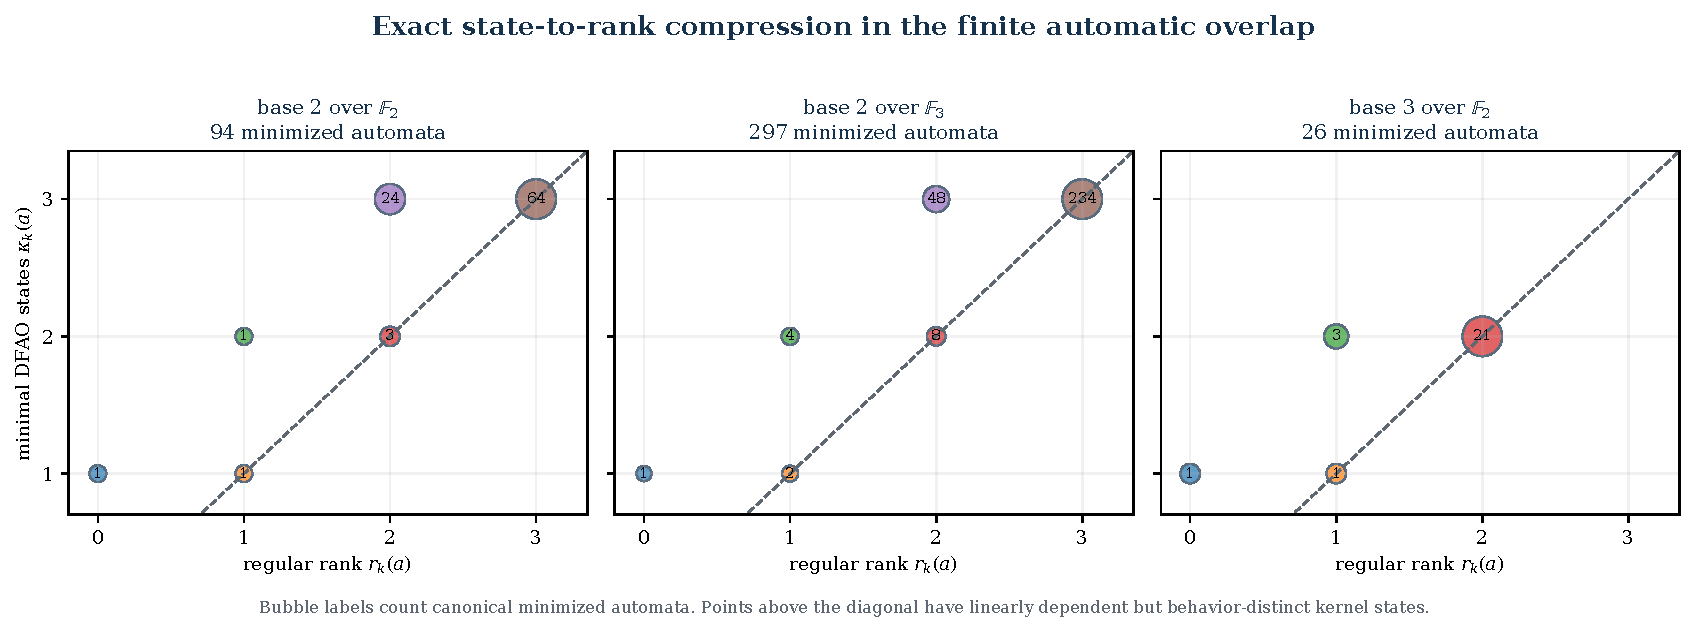
\includegraphics[width=0.99\textwidth]{automatic_regular_rank_distribution.pdf}
\caption{Exact bounded enumeration of the automatic overlap.  Bubble labels count distinct minimized automata.  Points above the diagonal are finite kernel orbits whose state behaviors are distinct but linearly dependent.}
\label{fig:automatic-regular-rank-distribution}
\end{figure}

The corollary explains why deterministic state minimization and linear-state minimization must remain distinct coordinates.  The minimal automaton records the finite orbit as a set with digit action.  The regular rank records the dimension of its linear span.  Neither number alone reconstructs the other.

\subsection{Exact regular examples beyond automaticity}

Over an infinite field, finite linear rank does not force a finite section orbit.  The following families give exact, unbounded witnesses.

\begin{theorem}[Polynomial regular rank in characteristic zero]
\label{thm:block05-polynomial-rank}
Let \(K\) have characteristic zero and let \(P\in K[x]\) be nonzero of degree \(m\).  For the sequence \(a_n=P(n)\),
\[
r_k(a)=m+1.
\]
If \(m\geq1\), its \(k\)-kernel is infinite.
\end{theorem}

\begin{proof}
Every section has the form
\[
(\Lambda_wa)(n)
=
P(k^{|w|}n+[w]_k),
\]
which is a polynomial in \(n\) of degree at most \(m\).  Hence the section span has dimension at most \(m+1\).

Choose \(\ell\) with \(k^\ell>m\) and consider the \(m+1\) sections
\[
P(k^\ell n+r),
\qquad 0\leq r\leq m.
\]
When expanded in the basis \(1,n,\ldots,n^m\), their coefficient functions as functions of \(r\) have successive degrees \(m,m-1,\ldots,0\), with nonzero leading coefficients.  Evaluation at the distinct points \(0,1,\ldots,m\) therefore gives an invertible generalized Vandermonde matrix.  These sections are linearly independent, proving rank \(m+1\).

For \(m\geq1\), the sections \(P(k^\ell n+r)\) are distinct as \(r\) varies through arbitrarily large complete residue ranges, so the kernel orbit is infinite.
\end{proof}

\begin{corollary}
For \(a_n=n\), one has \(r_k(a)=2\) and exactly \(k^\ell\) distinct sections at depth \(\ell\).  For \(a_n=n^2\), one has \(r_k(a)=3\) and again exactly \(k^\ell\) distinct sections at depth \(\ell\).
\end{corollary}

\begin{theorem}[Digit-sum regularity]
\label{thm:block05-digit-sum}
Let \(s_k(n)\) be the sum of the base-\(k\) digits of \(n\), regarded as a sequence over a characteristic-zero field.  Then
\[
r_k(s_k)=2,
\]
and
\begin{equation}
\mathcal K_k(s_k)
=
\{s_k+c:c\in\mathbb Z_{\geq0}\}.
\label{eq:block05-digit-sum-kernel}
\end{equation}
At exact depth \(\ell\), the number of distinct sections is
\[
(k-1)\ell+1.
\]
Thus \(s_k\) is \(k\)-regular but not \(k\)-automatic over a characteristic-zero field.
\end{theorem}

\begin{proof}
The digit identity
\[
s_k(kn+d)=s_k(n)+d
\]
gives
\[
\Lambda_d s_k=s_k+d.
\]
Iterating shows that every section is \(s_k+c\), so the span is contained in \(\Span\{1,s_k\}\).  The two sequences are independent, giving rank two.  At depth \(\ell\), the additive constant is the digit sum of an \(\ell\)-digit residue.  Every integer from \(0\) through \((k-1)\ell\) occurs, giving exactly \((k-1)\ell+1\) states.
\end{proof}

\begin{table}[htbp]
\centering
\caption{Named examples at the automatic--regular boundary.}
\label{tab:block05-examples}
\small
\begin{tabularx}{\textwidth}{@{}L{0.25\textwidth}L{0.13\textwidth}L{0.11\textwidth}L{0.13\textwidth}Y@{}}
\toprule
Example & Base / field & Regular rank & Kernel or states & Classification\\
\midrule
Ternary Cantor-digit indicator & 3 / $\mathbb F_3$ & 1 & 2 & automatic and regular\\
Thue-Morse parity & 2 / $\mathbb F_2$ & 2 & 2 & automatic and regular\\
Identity sequence $n$ & 2 / $\mathbb Q$ & 2 & infinite & regular, not automatic\\
Binary digit sum $s_2(n)$ & 2 / $\mathbb Q$ & 2 & infinite & regular, not automatic\\
Square sequence $n^2$ & 2 / $\mathbb Q$ & 3 & infinite & regular, not automatic\\
\bottomrule
\end{tabularx}
\end{table}


\begin{figure}[htbp]
\centering
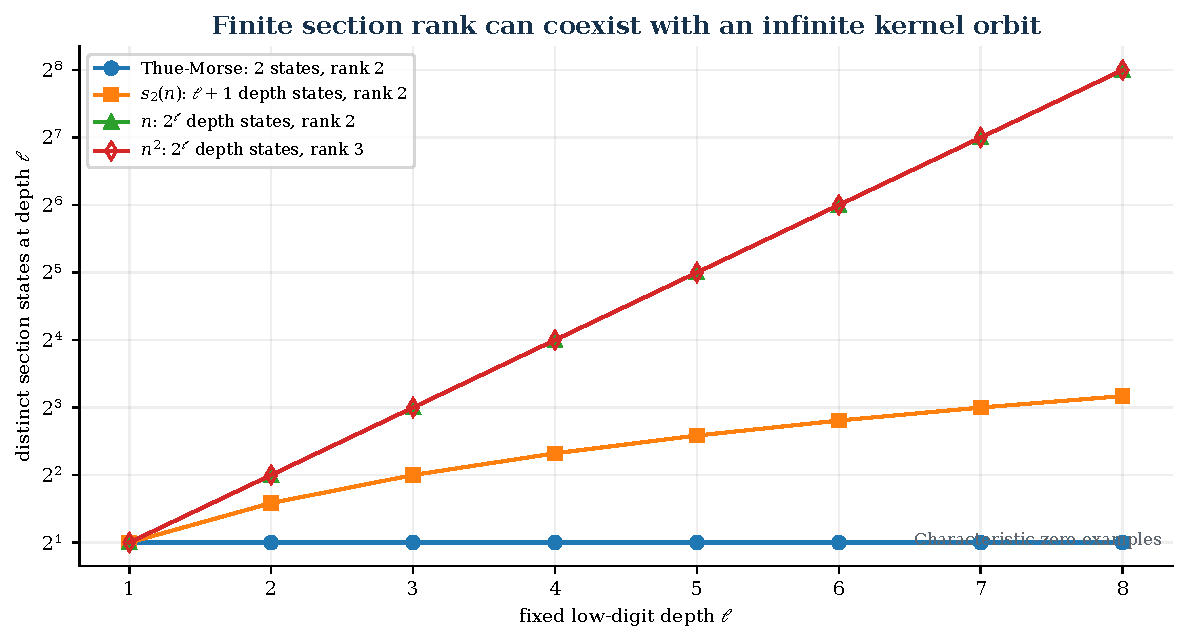
\includegraphics[width=0.99\textwidth]{regular_infinite_orbit_examples.pdf}
\caption{Fixed section rank does not bound orbit cardinality over an infinite field.  The Thue--Morse orbit is finite, while \(n\), \(n^2\), and the digit sum have finite linear rank but unboundedly many distinct sections.}
\label{fig:regular-infinite-orbit}
\end{figure}

\subsection{Exact finite verification}

\begin{table}[htbp]
\centering
\caption{Exact finite validation of the Fixed-radix regular atlas fixed-radix regular atlas.}
\label{tab:block05-validation}
\small
\begin{tabularx}{\textwidth}{@{}L{0.27\textwidth}Y@{}}
\toprule
Check & Recorded result\\
\midrule
Exhaustive finite-state enumeration & base 2 over $\mathbb F_2$ through 3 raw states: 5,898 raw candidates, 2,830 leading-zero-consistent candidates, 94 distinct minimized automata; base 2 over $\mathbb F_3$ through 3 raw states: 19,830 raw candidates, 6,990 leading-zero-consistent candidates, 297 distinct minimized automata; base 3 over $\mathbb F_2$ through 2 raw states: 258 raw candidates, 170 leading-zero-consistent candidates, 26 distinct minimized automata.\\
Automatic-to-linear checks & 86,207 exact checks; 83 minimized automata with strict state-to-rank compression.\\
Unbounded regular examples & Polynomial sequences $n^m$ for bases 2 and 3 through degree 6, plus digit sums in bases 2, 3, and 4; 2,438 exact checks.\\
Combined Fixed-radix regular atlas checks & 89,055 checks; 0 failures.\\
Overall status & PASS.\\
Boundary & The computation validates the bounded automata and named exact examples. It does not prove an all-radix, all-ring, semiring, or all-moduli minimality theorem.\\
\bottomrule
\end{tabularx}
\end{table}


The Fixed-radix regular atlas verifier performs two complementary exact audits.

First, it exhaustively enumerates bounded deterministic automata in three configurations:
\[
(k,q,s_{\max})=(2,2,3),\qquad(2,3,3),\qquad(3,2,2).
\]
Every candidate is restricted to reachable states, minimized by behavioral equivalence, and filtered by the terminal-high-zero consistency required by integer semantics.  For every resulting normalized automaton the verifier checks:
\begin{enumerate}
\item reachability and pairwise behavioral distinguishability;
\item construction of the canonical linear quotient from continuation-output rows;
\item transition and output equivariance of the state embedding;
\item the inequalities in \cref{eq:block05-state-rank-bound};
\item equality of word-Hankel rank and regular rank;
\item exact equality between the finite linear orbit and the minimized automaton state set;
\item coefficient agreement on a fixed exact test range.
\end{enumerate}

Second, it checks unbounded symbolic families using exact integer and rational matrices.  Polynomial sequences \(n^m\) are checked for bases two and three through degree six, and digit sums are checked in bases two, three, and four, including their exact depth-orbit growth formulas.

The finite audit records 89,055 exact checks and no failures.  It supports the implementation, examples, and bounded state-rank distribution.  The unbounded theorems above are proved symbolically and do not depend on the enumeration.

\begin{boundarybox}
\textbf{Exact boundary of Fixed-radix regular atlas.}
The normalization theorem is fixed-radix and field-valued.  It does not yet give one integral normal form valid simultaneously modulo every prime power, a semiring minimality theorem, or a canonical all-radix comparison invariant.  Over a general commutative ring, the section module can have torsion, fail to be free, and admit inequivalent minimal generating systems.  Saturation, Smith/Fitting data, prime-power reduction towers, and local completion therefore remain separate arithmetic obligations rather than being hidden inside the field theorem.
\end{boundarybox}

\begin{resultbox}
\textbf{Section result.}
Every field-valued fixed-radix regular sequence has a canonical section module, a minimal reachable-observable digit-linear realization, an exact word-Hankel rank, and a strict shortlex normal form.  These charts satisfy effective normalized descent and yield a complete invariant on the declared fixed-radix regular category.  The automatic locus is exactly the finite-orbit locus inside the same module, where the minimal DFAO is recovered as the orbit of the distinguished initial vector.  Over finite fields regularity and automaticity coincide, while over characteristic-zero fields polynomial and digit-sum examples have finite rank and infinite section orbit.  This closes fixed-radix linear-state minimality over fields, not the all-moduli or integral regular-sequence problem.
\end{resultbox}


\section{Integral saturation, Smith--Fitting defects, and prime-power effectivity}
\label{sec:block06-integral-prime-power}

Fixed-radix regular atlas proves a complete fixed-radix normalization theorem over a field.  The next question is not obtained by replacing the coefficient field with \(\mathbb Z\) symbol by symbol.  Over \(\mathbb Z\), two canonical lattices appear inside the same rational section space.  Their finite-index difference is invisible over \(\mathbb Q\), but it controls reduction modulo every integer, the appearance of ghost coordinates, and the distinction between an effective \(p\)-adic lift and an effective integral lift.

Throughout this section, \(k\geq2\) is fixed and
\[
a:\mathbb N\longrightarrow\mathbb Z
\]
is an integer-valued sequence whose rational section space
\[
V_{\mathbb Q}(a)
=
\operatorname{span}_{\mathbb Q}\mathcal K_k(a)
\subseteq
\mathbb Q^{\mathbb N}
\]
has finite dimension
\[
\rho_k(a)=\dim_{\mathbb Q}V_{\mathbb Q}(a).
\]
Thus \(a\) is \(k\)-regular after extension of scalars to \(\mathbb Q\).

\subsection{The raw section lattice and its canonical saturation}

\begin{definition}[Raw and saturated section lattices]
\label{def:block06-lattices}
The \emph{raw section lattice} and the \emph{saturated section lattice} are
\[
M_k(a)
=
\operatorname{span}_{\mathbb Z}\mathcal K_k(a),
\qquad
L_k(a)
=
V_{\mathbb Q}(a)\cap\mathbb Z^{\mathbb N}.
\]
The intersection defining \(L_k(a)\) is taken inside \(\mathbb Q^{\mathbb N}\).
\end{definition}

The raw lattice is generated by the actual radix sections.  The saturated lattice contains every integer-valued sequence lying in their rational span.  These lattices agree over \(\mathbb Q\), but need not agree over \(\mathbb Z\).

\begin{lemma}[Finite coordinate detection]
\label{lem:block06-coordinate-detection}
Let \(V\subseteq\mathbb Q^{\mathbb N}\) be a vector space of finite dimension \(\rho\).  There exist indices
\[
0\leq n_1<\cdots<n_\rho
\]
such that the evaluation map
\[
E_{\mathbf n}:V\longrightarrow\mathbb Q^\rho,
\qquad
f\longmapsto
\bigl(f(n_1),\ldots,f(n_\rho)\bigr)
\]
is an isomorphism.
\end{lemma}

\begin{proof}
The coordinate functionals on \(\mathbb Q^{\mathbb N}\) separate points of \(V\).  Choose \(n_1\) for which some element of \(V\) has nonzero value.  If \(n_1,\ldots,n_j\) have been chosen and the joint evaluation map has rank \(j<\rho\), its kernel contains a nonzero \(f\).  Choose \(n_{j+1}\) with \(f(n_{j+1})\neq0\).  The rank increases.  After \(\rho\) steps, the evaluation map has full rank.
\end{proof}

\begin{theorem}[Canonical finite saturated section lattice]
\label{thm:block06-saturation}
The groups \(M_k(a)\) and \(L_k(a)\) are free abelian of rank \(\rho_k(a)\).  They are stable under every digit section \(\Lambda_d\), and
\[
M_k(a)\subseteq L_k(a)
\]
has finite index.  Moreover, \(L_k(a)\) is the unique maximal subgroup of \(V_{\mathbb Q}(a)\) whose elements are integer-valued.
\end{theorem}

\begin{proof}
Choose a coordinate-detection set \(\mathbf n\) by \cref{lem:block06-coordinate-detection}.  Evaluation embeds \(L_k(a)\) into \(\mathbb Z^\rho\), so \(L_k(a)\) is a finitely generated free abelian group of rank at most \(\rho\).  The raw lattice \(M_k(a)\) is contained in \(L_k(a)\), and its rational span is all of \(V_{\mathbb Q}(a)\).  Hence \(M_k(a)\) has rank \(\rho\), and therefore \(L_k(a)\) also has rank \(\rho\).  A subgroup of a finitely generated free abelian group is finitely generated and free, so \(M_k(a)\) is free of rank \(\rho\).  Equal-rank lattice inclusion has finite index.

Every \(\Lambda_d\) preserves \(V_{\mathbb Q}(a)\) and preserves integer-valued sequences.  Hence it preserves \(L_k(a)\).  It also maps each radix section to another radix section, so it preserves \(M_k(a)\).  Finally, any integer-valued subgroup of \(V_{\mathbb Q}(a)\) lies in \(V_{\mathbb Q}(a)\cap\mathbb Z^{\mathbb N}=L_k(a)\).
\end{proof}

\begin{definition}[Integral saturation defect]
\label{def:block06-defect}
The finite abelian group
\[
C_k(a)
=
L_k(a)/M_k(a)
\]
is the \emph{integral saturation defect}.  Its order
\[
\delta_k(a)
=
[L_k(a):M_k(a)]
\]
is the \emph{saturation index}.
\end{definition}

By the Smith normal form, there are uniquely determined integers
\[
1\leq d_1(a)\mid d_2(a)\mid\cdots\mid d_{\rho}(a)
\]
such that
\[
C_k(a)
\cong
\bigoplus_{i=1}^{\rho}\mathbb Z/d_i(a)\mathbb Z.
\]
Factors with \(d_i=1\) are harmless but are retained so that the list has length \(\rho\).

\begin{figure}[htbp]
\centering
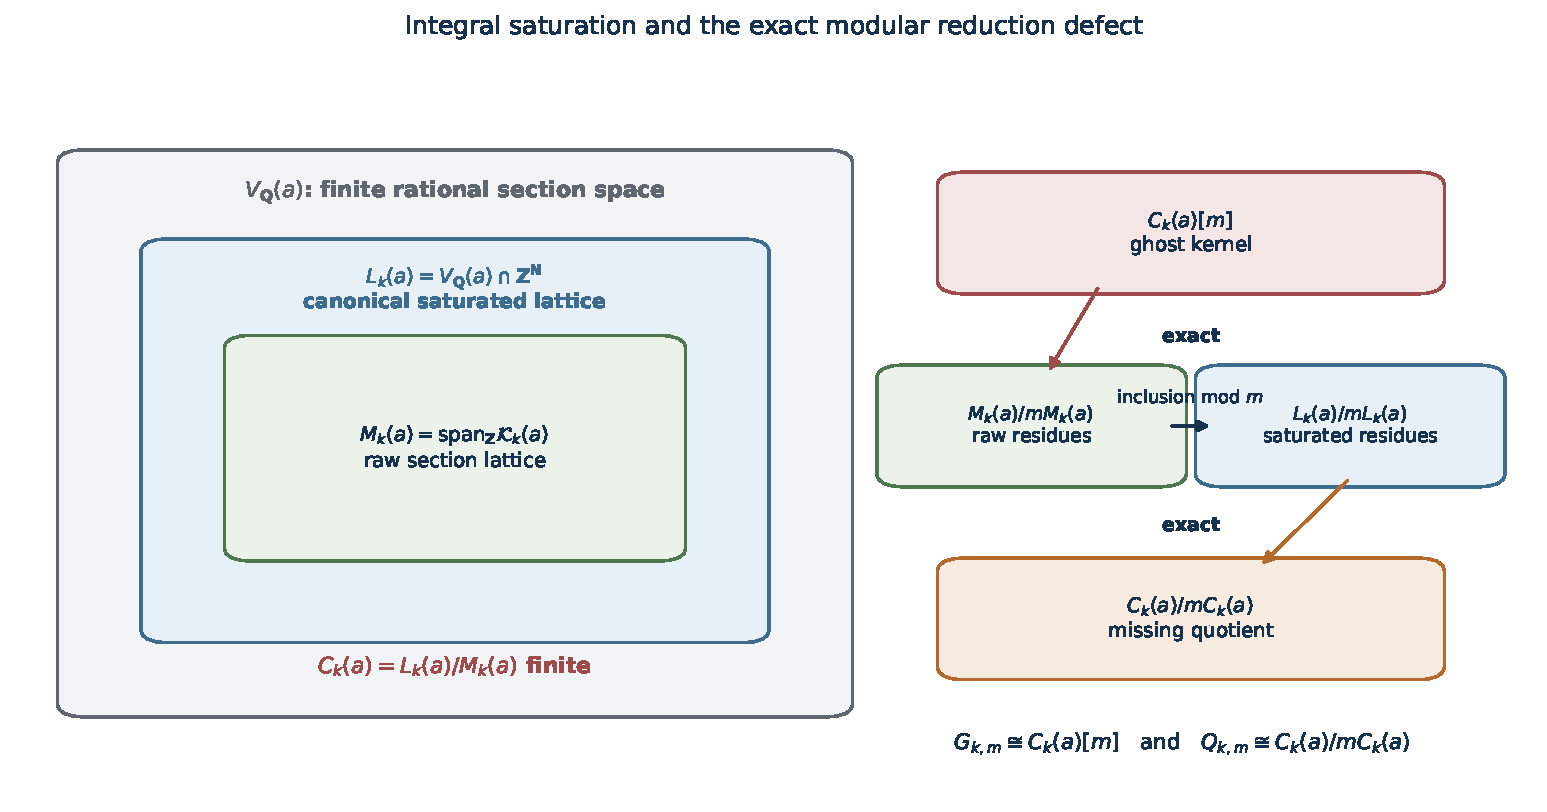
\includegraphics[width=.93\textwidth]{saturation_reduction_defect.pdf}
\caption{The rational section space contains the raw section lattice and its canonical integer-valued saturation.  The finite quotient is invisible over \(\mathbb Q\), but it controls every modular reduction.}
\label{fig:block06-saturation-defect}
\end{figure}

\begin{example}[A rank-two nontrivial defect]
\label{ex:block06-double-digitsum}
Let \(s_k(n)\) be the base-\(k\) digit-sum sequence and let \(a=2s_k\).  Since
\[
\Lambda_d s_k=s_k+d,
\]
the rational section space is spanned by \(s_k\) and the constant sequence \(1\).  The actual sections of \(2s_k\) generate
\[
M_k(2s_k)
=
2\mathbb Z\,s_k\oplus2\mathbb Z\,1,
\]
whereas
\[
L_k(2s_k)
=
\mathbb Z\,s_k\oplus\mathbb Z\,1.
\]
Thus
\[
C_k(2s_k)
\cong
(\mathbb Z/2\mathbb Z)^2.
\]
The rational regular rank is two, but reduction modulo two loses the entire semantic lattice.
\end{example}

\subsection{The exact reduction sequence}

For an integer \(m\geq2\), the raw coefficient reduction is
\[
M_k(a)/mM_k(a),
\]
while the semantic reduction inside the saturated lattice is
\[
\overline M_{k,m}(a)
=
\operatorname{im}
\left(
M_k(a)/mM_k(a)
\longrightarrow
L_k(a)/mL_k(a)
\right).
\]
These need not agree.

\begin{definition}[Ghost and missing reduction modules]
\label{def:block06-ghost-missing}
Define
\[
G_{k,m}(a)
=
\ker
\left(
M_k(a)/mM_k(a)
\longrightarrow
L_k(a)/mL_k(a)
\right)
\]
and
\[
Q_{k,m}(a)
=
\operatorname{coker}
\left(
M_k(a)/mM_k(a)
\longrightarrow
L_k(a)/mL_k(a)
\right).
\]
The first records raw residue coordinates that represent the zero semantic sequence.  The second records saturated residue classes not reached by raw sections.
\end{definition}

\begin{theorem}[Smith--Tor reduction sequence]
\label{thm:block06-tor-sequence}
For every \(m\geq2\), tensoring
\[
0\longrightarrow M_k(a)\longrightarrow L_k(a)\longrightarrow C_k(a)\longrightarrow0
\]
with \(\mathbb Z/m\mathbb Z\) gives a canonical digit-equivariant exact sequence
\[
0
\longrightarrow
C_k(a)[m]
\longrightarrow
M_k(a)/mM_k(a)
\longrightarrow
L_k(a)/mL_k(a)
\longrightarrow
C_k(a)/mC_k(a)
\longrightarrow
0.
\]
Consequently,
\[
G_{k,m}(a)\cong C_k(a)[m],
\qquad
Q_{k,m}(a)\cong C_k(a)/mC_k(a).
\]
\end{theorem}

\begin{proof}
Both \(M_k(a)\) and \(L_k(a)\) are free abelian.  The long exact Tor sequence therefore begins
\[
0\longrightarrow
\operatorname{Tor}_1^{\mathbb Z}
(C_k(a),\mathbb Z/m\mathbb Z)
\longrightarrow
M_k(a)\otimes\mathbb Z/m\mathbb Z
\longrightarrow
L_k(a)\otimes\mathbb Z/m\mathbb Z.
\]
For any abelian group \(C\),
\[
\operatorname{Tor}_1^{\mathbb Z}(C,\mathbb Z/m\mathbb Z)
\cong C[m],
\qquad
C\otimes\mathbb Z/m\mathbb Z
\cong C/mC.
\]
The digit-section maps preserve the original short exact sequence, so naturality of Tor makes the five-term sequence digit-equivariant.
\end{proof}

\begin{corollary}[Exact Smith formulas]
\label{cor:block06-smith-formulas}
Let \(g_i(m)=\gcd(m,d_i(a))\).  Then
\[
G_{k,m}(a)
\cong
Q_{k,m}(a)
\cong
\bigoplus_{i=1}^{\rho}
\mathbb Z/g_i(m)\mathbb Z,
\]
and
\[
\left|\overline M_{k,m}(a)\right|
=
\prod_{i=1}^{\rho}
\frac{m}{g_i(m)}.
\]
The reduction map is an isomorphism if and only if
\[
\gcd\bigl(m,d_\rho(a)\bigr)=1.
\]
Equivalently, every prime dividing a reduction defect divides the saturation index.
\end{corollary}

\begin{proof}
Choose Smith bases in which the inclusion \(M_k(a)\hookrightarrow L_k(a)\) is the diagonal matrix
\[
D=\operatorname{diag}(d_1,\ldots,d_\rho).
\]
Modulo \(m\), the kernel and cokernel of multiplication by \(d_i\) are both cyclic of order \(\gcd(m,d_i)\), and the image has order \(m/\gcd(m,d_i)\).  The map is invertible in every coordinate exactly when every \(d_i\) is a unit modulo \(m\), which is equivalent to \(\gcd(m,d_\rho)=1\).
\end{proof}

\begin{proposition}[Fitting-ideal certificate]
\label{prop:block06-fitting}
For \(0\leq j<\rho\),
\[
\operatorname{Fitt}_j(C_k(a))
=
\left(
d_1(a)d_2(a)\cdots d_{\rho-j}(a)
\right),
\]
and
\[
\operatorname{Fitt}_j(C_k(a))=\mathbb Z
\qquad
(j\geq\rho).
\]
Thus the Smith profile and the Fitting filtration contain the same reduction-defect data at different resolutions.
\end{proposition}

\begin{proof}
Use the diagonal presentation \(D:\mathbb Z^\rho\to\mathbb Z^\rho\).  The \(j\)-th Fitting ideal is generated by the minors of size \(\rho-j\).  Since \(d_1\mid\cdots\mid d_\rho\), the product of the first \(\rho-j\) diagonal entries divides every other such minor and is itself one of the minors.
\end{proof}

\begin{boundary}[What the defect classifies]
\label{bnd:block06-defect-boundary}
The group \(C_k(a)\) classifies the finite-index failure of the raw section lattice to be saturated.  It does not classify the whole integral digit module, the sequence, or its section orbit.  Two nonisomorphic digit modules can have the same Smith profile.
\end{boundary}

\subsection{Digit equivariance and the prime-power tower}

Choose Smith bases for \(M_k(a)\) and \(L_k(a)\), and let
\[
D=\operatorname{diag}(d_1,\ldots,d_\rho)
\]
be the inclusion matrix.  Let \(A_d\) and \(B_d\) be the integer matrices of \(\Lambda_d\) on the raw and saturated lattices.

\begin{proposition}[Intertwining across saturation]
\label{prop:block06-intertwining}
For every digit \(d\),
\[
B_dD=DA_d.
\]
Consequently, the raw modules, semantic images, ghost modules, and missing modules at every modulus form compatible digit modules.
\end{proposition}

\begin{proof}
The inclusion \(M_k(a)\hookrightarrow L_k(a)\) commutes with \(\Lambda_d\).  The displayed matrix identity is that commutative square in the chosen bases.  Reduction modulo \(m\), passage to kernel, image, and cokernel preserve the induced digit action.
\end{proof}

Fix a prime \(p\) and write
\[
\nu_i=\nu_{p,i}(a)=v_p(d_i(a)).
\]

\begin{theorem}[Prime-power defect profile]
\label{thm:block06-prime-power-profile}
For \(r\geq1\),
\[
G_{k,p^r}(a)
\cong
Q_{k,p^r}(a)
\cong
\bigoplus_{i=1}^{\rho}
\mathbb Z/p^{\min(r,\nu_i)}\mathbb Z,
\]
and
\[
\left|\overline M_{k,p^r}(a)\right|
=
p^{\sum_{i=1}^{\rho}(r-\min(r,\nu_i))}.
\]
The minimal number of generators of \(\overline M_{k,p^r}(a)\) as a \(\mathbb Z/p^r\mathbb Z\)-module is
\[
\mu_{p^r}(a)
=
\#\{i:\nu_i<r\}.
\]
In particular, \(p\) is a good reduction prime exactly when every \(\nu_i=0\).
\end{theorem}

\begin{proof}
Apply \cref{cor:block06-smith-formulas} to \(m=p^r\).  The \(i\)-th semantic image is the ideal
\[
p^{\min(r,\nu_i)}\mathbb Z/p^r\mathbb Z.
\]
It is nonzero and cyclic exactly when \(\nu_i<r\).  Over the local ring \(\mathbb Z/p^r\mathbb Z\), the minimal number of generators of a direct sum of cyclic ideals is the number of nonzero summands.
\end{proof}

\begin{figure}[htbp]
\centering
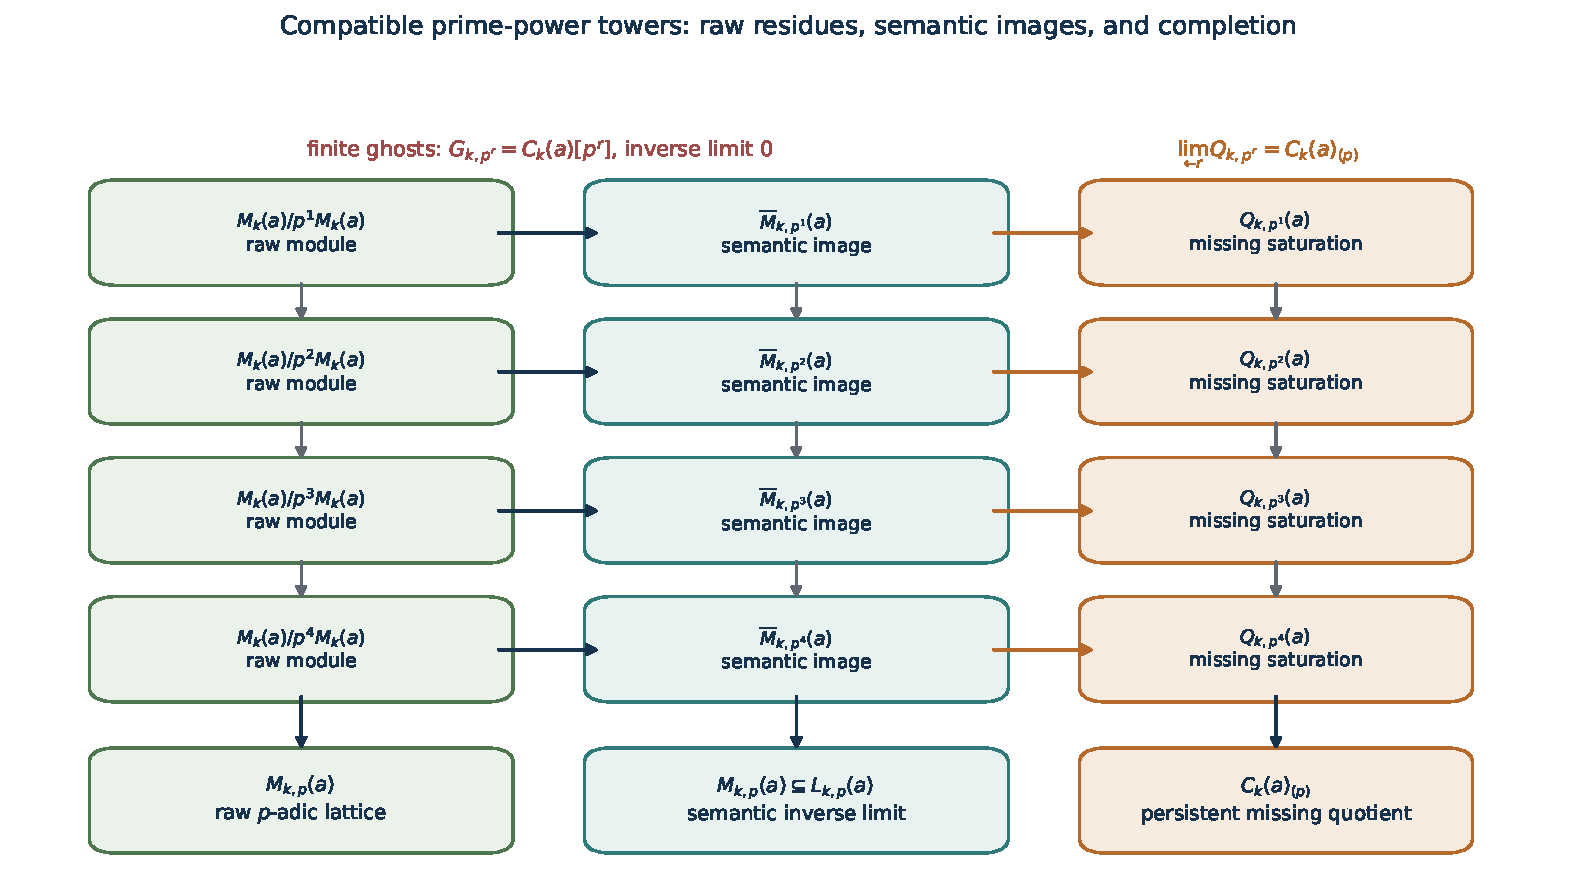
\includegraphics[width=.94\textwidth]{prime_power_regular_tower.pdf}
\caption{The raw residue tower maps onto the semantic prime-power tower.  Ghost coordinates occur at finite depth when the raw lattice is not \(p\)-saturated.  The compatible semantic tower converges to the embedded \(p\)-adic raw lattice.}
\label{fig:block06-prime-power-tower}
\end{figure}

\begin{definition}[Prime-power section automaton]
\label{def:block06-prime-power-automaton}
The semantic \(p^r\)-kernel is
\[
\mathcal K_{k,p^r}^{\mathrm{sem}}(a)
=
\left\{
\Lambda_w a\bmod p^rL_k(a):
w\in\Sigma_k^*
\right\}
\subseteq
\overline M_{k,p^r}(a).
\]
Its cardinality is denoted
\[
\kappa_{k,p^r}^{\mathrm{sem}}(a).
\]
\end{definition}

\begin{theorem}[Finite prime-power automata]
\label{thm:block06-prime-power-automata}
For every \(r\geq1\), the semantic \(p^r\)-kernel is finite and is the state set of the unique minimal least-significant-digit-first deterministic output automaton for the coefficient sequence \(a\bmod p^r\).  Moreover,
\[
\kappa_{k,p^r}^{\mathrm{sem}}(a)
\leq
\left|\overline M_{k,p^r}(a)\right|
=
p^{\sum_i(r-\min(r,\nu_i))}.
\]
Reduction induces surjective digit-equivariant maps
\[
\mathcal K_{k,p^{r+1}}^{\mathrm{sem}}(a)
\twoheadrightarrow
\mathcal K_{k,p^r}^{\mathrm{sem}}(a).
\]
\end{theorem}

\begin{proof}
The semantic section module is finite, so its orbit under the digit maps is finite.  As in the field-valued proof of \cref{thm:block05-kernel-automaton}, every orbit state is reachable.  Distinct section sequences have a continuation on which they differ, so they are behaviorally distinguishable.  This gives the minimal deterministic automaton.  The cardinality bound is the ambient module bound.  The same section word at level \(r+1\) reduces to the corresponding section word at level \(r\), so the transition map on orbit states is surjective.
\end{proof}

\begin{corollary}[Good-prime transfer]
\label{cor:block06-good-prime}
If \(p\nmid\delta_k(a)\), then for every \(r\geq1\),
\[
M_k(a)/p^rM_k(a)
\overset{\sim}{\longrightarrow}
\overline M_{k,p^r}(a)
=
L_k(a)/p^rL_k(a).
\]
At a good prime, the raw and saturated prime-power towers agree exactly.
\end{corollary}

\begin{table}[htbp]
\centering
\caption{Canonical integral defect profiles for named fixed-radix families.}
\label{tab:block06-defect-profiles}
\small
\begin{tabularx}{\textwidth}{@{}L{0.22\textwidth}L{0.17\textwidth}L{0.18\textwidth}Y@{}}
\toprule
Family & Smith profile & Bad primes & Interpretation\\
\midrule
Digit sum $s_k$ & $(1,1)$ & none & Saturated rank-two lattice; no modular defect.\\
Doubled digit sum $2s_k$ & $(2,2)$ & 2 & Rank-two defect $(\mathbb Z/2)^2$; total semantic collapse modulo $2$.\\
Constant sequence $2$ & $(2)$ & 2 & One raw ghost coordinate modulo $2$; one semantic state.\\
Constant sequence $6$ & $(6)$ & 2, 3 & Bad primes $2$ and $3$; good reduction at every other prime.\\
\bottomrule
\end{tabularx}
\end{table}


\subsection{p-adic completion and the disappearance of finite ghosts}

Define
\[
M_{k,p}(a)=M_k(a)\otimes_{\mathbb Z}\mathbb Z_p,
\qquad
L_{k,p}(a)=L_k(a)\otimes_{\mathbb Z}\mathbb Z_p.
\]

\begin{theorem}[\(p\)-adic saturation sequence]
\label{thm:block06-padic-saturation}
There is a digit-equivariant short exact sequence
\[
0
\longrightarrow
M_{k,p}(a)
\longrightarrow
L_{k,p}(a)
\longrightarrow
C_k(a)_{(p)}
\longrightarrow
0,
\]
where \(C_k(a)_{(p)}\) is the \(p\)-primary subgroup of \(C_k(a)\).  In Smith coordinates,
\[
M_{k,p}(a)
=
\bigoplus_{i=1}^{\rho}p^{\nu_i}\mathbb Z_p e_i
\subseteq
\bigoplus_{i=1}^{\rho}\mathbb Z_p e_i
=
L_{k,p}(a).
\]
\end{theorem}

\begin{proof}
The \(\mathbb Z\)-module \(\mathbb Z_p\) is torsion free and hence flat.  Tensor the integral short exact sequence with \(\mathbb Z_p\).  For a finite abelian group \(C\),
\[
C\otimes_{\mathbb Z}\mathbb Z_p\cong C_{(p)}.
\]
The Smith-coordinate formula follows by tensoring the diagonal inclusion.
\end{proof}

\begin{theorem}[Raw and semantic inverse limits]
\label{thm:block06-inverse-limits}
There are canonical digit-equivariant identifications
\[
\varprojlim_r M_k(a)/p^rM_k(a)
\cong
M_{k,p}(a)
\]
and
\[
\varprojlim_r \overline M_{k,p^r}(a)
\cong
M_{k,p}(a)
\subseteq
L_{k,p}(a).
\]
Furthermore,
\[
\varprojlim_r G_{k,p^r}(a)=0,
\qquad
\varprojlim_r Q_{k,p^r}(a)
\cong
C_k(a)_{(p)}.
\]
\end{theorem}

\begin{proof}
The first identification is the definition of the \(p\)-adic completion of a finite free lattice.  In Smith coordinate \(i\), the semantic image at level \(r\) is
\[
p^{\min(r,\nu_i)}\mathbb Z/p^r\mathbb Z.
\]
Its inverse limit is \(p^{\nu_i}\mathbb Z_p\), giving the second identification.

A compatible ghost tower represents an element \(x\in\mathbb Z_p\) satisfying \(p^{\nu_i}x=0\).  Since \(\mathbb Z_p\) is torsion free, \(x=0\).  Hence the inverse limit of the ghost modules vanishes.  The missing quotient stabilizes coordinatewise at \(\mathbb Z/p^{\nu_i}\mathbb Z\), whose product is the \(p\)-primary Smith quotient.
\end{proof}

The finite ghosts are therefore real finite-level defects, but they do not survive as nonzero points of the completed raw lattice.  By contrast, the missing saturated quotient survives exactly as the \(p\)-primary saturation defect.

\subsection{Orbit closure and three levels of effectivity}

Let
\[
\mathcal O_k(a)=\{\Lambda_w a:w\in\Sigma_k^*\}\subseteq M_k(a)
\]
be the actual section orbit, and let
\[
\mathcal O^{\mathrm{raw}}_{k,p^r}(a)
\]
be its image in \(M_k(a)/p^rM_k(a)\).

\begin{theorem}[Raw orbit-closure descent]
\label{thm:block06-orbit-closure}
The reduction maps
\[
\mathcal O^{\mathrm{raw}}_{k,p^{r+1}}(a)
\twoheadrightarrow
\mathcal O^{\mathrm{raw}}_{k,p^r}(a)
\]
are surjective, and
\[
\overline{\mathcal O_k(a)}^{\,p}
\overset{\sim}{\longrightarrow}
\varprojlim_r
\mathcal O^{\mathrm{raw}}_{k,p^r}(a),
\]
where the closure is taken in \(M_{k,p}(a)\).
\end{theorem}

\begin{proof}
A section word at level \(r\) is lifted by the same word at level \(r+1\), proving surjectivity.  Every \(p\)-adic limit of orbit points gives a compatible tower.  Conversely, choose for each compatible residue state an orbit representative \(x_r\).  Compatibility gives
\[
x_{r+1}-x_r\in p^rM_k(a),
\]
so \((x_r)\) is Cauchy in \(M_{k,p}(a)\).  Its limit lies in the orbit closure and maps to the prescribed tower.
\end{proof}

\begin{definition}[Three effectivity obstructions]
\label{def:block06-effectivity}
Let \(x\in M_{k,p}(a)\).
\begin{enumerate}
\item The \emph{\(p\)-adic effectivity condition} is simply \(x\in M_{k,p}(a)\); every compatible full semantic module tower satisfies it by \cref{thm:block06-inverse-limits}.
\item The \emph{integral lattice obstruction} is
\[
\epsilon_{\mathrm{int}}(x)
=
[x]\in M_{k,p}(a)/M_k(a).
\]
It vanishes exactly when \(x\) is represented by one integral lattice element.
\item The \emph{section-orbit obstruction} is membership in
\[
M_k(a)\setminus\mathcal O_k(a).
\]
Even after integral effectivity holds, the lift need not be an actual radix section.
\end{enumerate}
\end{definition}

\begin{boundary}[Semantic orbit towers]
\label{bnd:block06-semantic-orbit}
The inverse limit of the full semantic modules is always \(M_{k,p}(a)\).  For the smaller semantic orbit sets, surjectivity of reduction remains automatic, but lifting to an actual orbit closure can be obscured by finite ghost fibers.  The unconditional orbit-closure theorem is therefore stated for the raw orbit tower.  A semantic-orbit effectivity theorem requires a compatible choice of raw lifts or an equivalent fiberwise Mittag--Leffler condition.
\end{boundary}

\begin{example}[Digit sum separates all three levels]
\label{ex:block06-digitsum-effectivity}
For the base-\(k\) digit sum \(s_k\),
\[
\mathcal O_k(s_k)
=
\{s_k+c:c\in\mathbb Z_{\geq0}\},
\]
and
\[
M_k(s_k)=L_k(s_k)=\mathbb Zs_k\oplus\mathbb Z1.
\]
Hence
\[
\overline{\mathcal O_k(s_k)}^{\,p}
=
\{s_k+c:c\in\mathbb Z_p\}.
\]
The partial sums
\[
c_N=\sum_{j=0}^{N}p^{2j}
\]
are nonnegative integers and therefore produce actual section states \(s_k+c_N\).  They converge in \(\mathbb Z_p\) to
\[
c_\infty
=
\frac{1}{1-p^2},
\]
which is not an ordinary integer.  Thus \(s_k+c_\infty\) is \(p\)-adically effective and lies in the orbit closure, but its integral obstruction is nonzero.

By contrast, \(s_k-1\) is an integral lattice point and lies in the \(p\)-adic orbit closure because \(-1\in\mathbb Z_p\) is a limit of nonnegative integers.  It is not an actual section, since every actual offset is nonnegative.  Integral effectivity therefore does not imply section-orbit effectivity.
\end{example}

\begin{figure}[htbp]
\centering
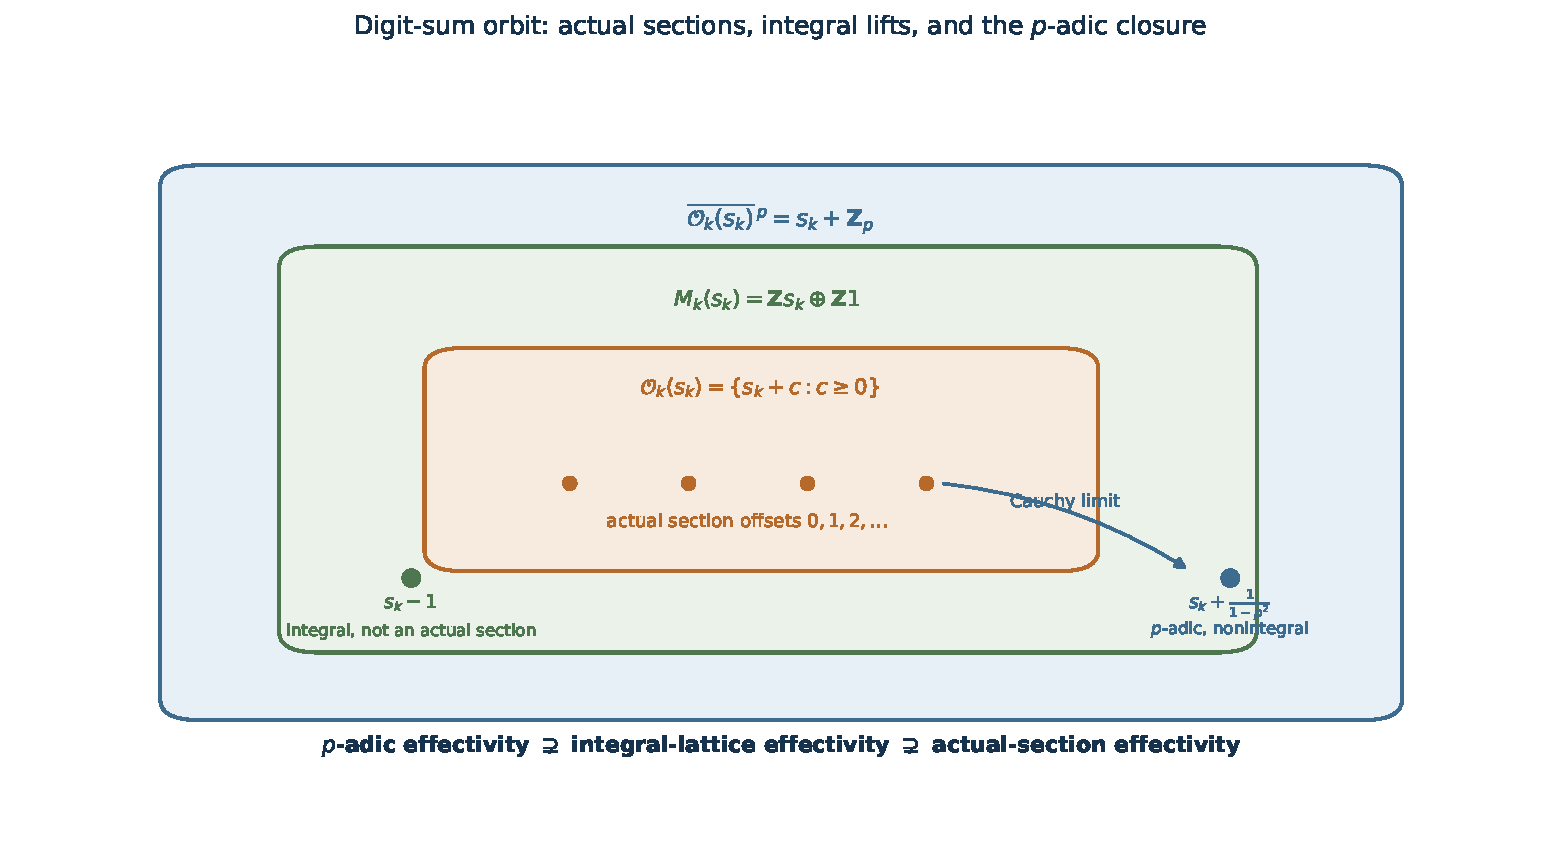
\includegraphics[width=.93\textwidth]{digit_sum_padic_effectivity.pdf}
\caption{For the digit-sum sequence, actual section states form a nonnegative integral ray.  Its \(p\)-adic closure contains all \(p\)-adic offsets, including nonintegral limits and integral points that are not actual sections.}
\label{fig:block06-digitsum-effectivity}
\end{figure}

\subsection{All-moduli completion and the integral effectivity obstruction}

Let
\[
\widehat{M_k(a)}
=
\varprojlim_m M_k(a)/mM_k(a)
\]
be the profinite completion over divisibility of moduli.

\begin{theorem}[Profinite saturation sequence]
\label{thm:block06-profinite}
There are canonical digit-equivariant identifications
\[
\widehat{M_k(a)}
\cong
\prod_p M_{k,p}(a),
\qquad
\widehat{L_k(a)}
\cong
\prod_p L_{k,p}(a),
\]
and a short exact sequence
\[
0
\longrightarrow
\widehat{M_k(a)}
\longrightarrow
\widehat{L_k(a)}
\longrightarrow
C_k(a)
\longrightarrow
0.
\]
A compatible all-moduli raw tower has an ordinary integral lift exactly when its class in
\[
\widehat{M_k(a)}/M_k(a)
\]
vanishes.
\end{theorem}

\begin{proof}
Finite free abelian groups have profinite completion equal to the product of their \(p\)-adic completions.  In Smith coordinates, the inclusion is multiplication by \(d_i\) in each profinite coordinate.  Its cokernel is
\[
\widehat{\mathbb Z}/d_i\widehat{\mathbb Z}
\cong
\mathbb Z/d_i\mathbb Z.
\]
Taking the direct sum over \(i\) gives \(C_k(a)\).  The final assertion is the definition of belonging to the diagonal image of the integral lattice inside its profinite completion.
\end{proof}

\begin{corollary}[Local-global separation]
\label{cor:block06-local-global}
Every compatible prime-power tower is effective in a \(p\)-adic completion.  A compatible family over all primes is effective in the profinite completion.  Neither statement alone implies an ordinary integral lift.  Integral effectivity is the separate diagonal condition
\[
\widehat{x}\in M_k(a)\subseteq\widehat{M_k(a)}.
\]
\end{corollary}

This is the precise sense in which prime-power effectivity and integral effectivity differ.  Completion solves the Cauchy problem in the declared topology.  It does not force the resulting point to lie in the original discrete lattice.

\subsection{Canonical integral record and directional reduction atlas}

\begin{definition}[Canonical integral regular record]
\label{def:block06-integral-record}
The canonical integral record of \(a\) is
\[
\mathcal I_k(a)
=
\left(
V_{\mathbb Q}(a),
M_k(a),
L_k(a),
C_k(a),
(\Lambda_d)_{0\leq d<k},
a,
\operatorname{ev}_0
\right).
\]
Its Smith--Fitting profile is
\[
\mathsf{SF}_k(a)
=
\left(
d_1,\ldots,d_\rho;
\operatorname{Fitt}_0(C_k(a)),\ldots,
\operatorname{Fitt}_{\rho-1}(C_k(a))
\right).
\]
\end{definition}

The record is canonical but not a single field-valued normal form.  It retains both the raw generative lattice and the maximal integer-valued lattice, together with the exact quotient between them.

\begin{theorem}[Integral normalization and directional local reduction]
\label{thm:block06-integral-normalization}
For fixed \(k\), the assignment
\[
a\longmapsto\mathcal I_k(a)
\]
is functorial for digit-module morphisms preserving the distinguished sequence and evaluation.  It is uniquely determined by the semantic sequence.  For every prime \(p\), reduction defines a directional bridge
\[
\mathcal I_k(a)
\longmapsto
\left(
\overline M_{k,p^r}(a),
\mathcal K_{k,p^r}^{\mathrm{sem}}(a)
\right)_{r\geq1}
\]
whose exact information-loss passport is:
\begin{enumerate}
\item finite-depth ghost kernel \(C_k(a)[p^r]\);
\item finite-depth missing quotient \(C_k(a)/p^rC_k(a)\);
\item completed essential image \(M_{k,p}(a)\subseteq L_{k,p}(a)\);
\item integral effectivity obstruction \(M_{k,p}(a)/M_k(a)\);
\item actual-section obstruction inside the integral lattice.
\end{enumerate}
\end{theorem}

\begin{proof}
Every component of \(\mathcal I_k(a)\) is defined from the semantic sequence and its digit sections.  A compatible morphism carries actual sections to actual sections and integer-valued rational combinations to integer-valued rational combinations, so it induces maps on \(M_k(a)\), \(L_k(a)\), and the quotient.  The local reduction statements are \cref{thm:block06-tor-sequence,thm:block06-inverse-limits,def:block06-effectivity}.
\end{proof}

\begin{resultbox}
\textbf{Section result.}
For every integer-valued fixed-radix sequence that is regular over \(\mathbb Q\), the actual sections generate a canonical finite free lattice \(M_k(a)\), and the integer-valued part of the rational section space is a canonical finite free saturation \(L_k(a)\).  Their Smith--Fitting quotient controls every modular reduction exactly.  At each prime power, the coefficient sequence has a finite minimal semantic section automaton.  The compatible tower reconstructs the \(p\)-adic raw lattice, while finite ghost coordinates vanish in the inverse limit and the missing saturated quotient survives as the \(p\)-primary defect.  \(p\)-adic, profinite, integral-lattice, and actual-section effectivity are distinct and are separated by explicit obstruction quotients.
\end{resultbox}

\begin{table}[htbp]
\centering
\caption{Exact finite validation of the Integral prime-power atlas integral and prime-power layer.}
\label{tab:block06-validation}
\small
\begin{tabularx}{\textwidth}{@{}L{0.31\textwidth}Y@{}}
\toprule
Check family & Recorded result\\
\midrule
Smith and modular profiles & 1984 divisibility chains of ranks one through four; moduli 2 through 24; 45632 chain-modulus cases.\\
Fitting and prime-power profiles & 8840 Fitting cases and 39680 prime-power profile cases over $p=2,3,5,7$.\\
Digit-equivariant systems & 320 exact Smith-square systems with integral and modular intertwining checks.\\
Orbit and completion controls & Digit-sum state formulas over four primes and 1681 bounded ghost-contraction samples.\\
Total exact checks & 697958; 0 failures.\\
Overall status & PASS.\\
Boundary & Bounded exact verification supports the printed formulas and examples. It does not replace the symbolic proofs or establish unrestricted integral recognition.\\
\bottomrule
\end{tabularx}
\end{table}


\begin{boundarybox}
\textbf{Exact boundary of Integral prime-power atlas.}
The results classify saturation and reduction defects for integer-valued sequences that are already known to have finite rational section rank.  They do not prove finite-data recognition of that hypothesis, a minimal realization theorem over arbitrary rings or semirings, a base-independent integral normal form, or compatibility across different radices.  The prime-power tower is a directional local reduction system, not an equivalence between integral and modular presentations.
\end{boundarybox}


\section{Filtered Euler products, prime-power seeds, and the divisor--ghost bridge}
\label{sec:block07-product-multiplicative}

The next native-invariant layer has two different index monoids.  Ordinary generating functions use the additive monoid of coefficient addresses: Cauchy multiplication combines indices by addition.  Arithmetic functions use the multiplicative monoid of positive integers: Dirichlet convolution combines divisor addresses by multiplication.  These structures meet exactly in selected local and logarithmic-derivative coordinates, but they are not globally interchangeable.  This section constructs the fixed-basis filtered-product normal form, the prime-power normal form for multiplicative arithmetic functions, and one rigorously typed cross-stratum bridge between them.

\subsection{Filtered products and coefficient stabilization}

\begin{definition}[Coefficientwise filtered product]
Let $R$ be a commutative ring.  A filtered factor family is a sequence
\[
F_m(z)\in 1+z^{w(m)}R[[z]],
\qquad
w(m)\longrightarrow\infty.
\]
Its coefficientwise product is
\[
\prod_{m\geq1}F_m(z),
\]
where the coefficient of $z^N$ is computed from the finitely many factors satisfying $w(m)\leq N$.
\end{definition}

\begin{proposition}[Filtered product completion]
Every filtered factor family has a unique coefficientwise product in $1+zR[[z]]$.  For every $N$, the truncation modulo $z^{N+1}$ is equal to the product of the finitely many factors with $w(m)\leq N$.
\end{proposition}

\begin{proof}
Fix $N$.  Every factor with $w(m)>N$ is congruent to $1$ modulo $z^{N+1}$, so only finitely many factors can affect the coefficient prefix through degree $N$.  These finite products are compatible as $N$ increases.  Their inverse limit in the $z$-adic filtration is the required series.  Uniqueness follows because every coefficient is fixed at a finite stage.
\end{proof}

The proposition supplies existence and exact finite-prefix evaluation.  It does not assert that an arbitrary factor family is structurally compressed.  A finite grammar requires an effective rule for the factors and a proof of stabilization; otherwise the factor list can merely store the coefficient data in another form.

\subsection{Canonical Euler coordinates}

Let
\[
\mathcal U_{\mathbb Z}=1+z\mathbb Z[[z]]
\]
be the multiplicative group of integral unit series, and let
\[
\mathcal E_{\mathbb Z}=\mathbb Z^{\mathbb N_{\geq1}}
\]
be the additive group of integer exponent sequences.

\begin{definition}[Euler-coordinate map]
For $b=(b_m)_{m\geq1}\in\mathcal E_{\mathbb Z}$, define
\[
\mathcal E(b)(z)
=
\prod_{m\geq1}(1-z^m)^{-b_m}.
\]
The product is coefficientwise filtered because the $m$th factor is congruent to $1$ modulo $z^m$.
\end{definition}

\begin{theorem}[Integral Euler-coordinate classification]
\label{thm:block07-euler-classification}
The map
\[
\mathcal E:
(\mathcal E_{\mathbb Z},+)
\longrightarrow
(\mathcal U_{\mathbb Z},\cdot)
\]
is a group isomorphism.  Consequently, every $A(z)\in1+z\mathbb Z[[z]]$ has a unique representation
\[
\boxed{
A(z)=\prod_{m\geq1}(1-z^m)^{-b_m},
\qquad b_m\in\mathbb Z.
}
\]
\end{theorem}

\begin{proof}
Filtered multiplication gives
\[
\mathcal E(b+b')=\mathcal E(b)\mathcal E(b').
\]
To prove surjectivity and uniqueness, construct the exponents recursively.  Suppose $b_1,\ldots,b_{n-1}$ have been chosen so that
\[
A(z)\prod_{m<n}(1-z^m)^{b_m}
\equiv 1+r_nz^n\pmod{z^{n+1}}.
\]
Because
\[
(1-z^n)^{-r_n}\equiv1+r_nz^n\pmod{z^{n+1}},
\]
the unique choice $b_n=r_n$ cancels the degree-$n$ residual.  Every $r_n$ is integral because all preceding operations occur in $\mathbb Z[[z]]$.  Induction produces one exponent sequence with the required product.  If two exponent sequences differed first at $n$, their quotient would have nonzero coefficient $(b_n-b_n')z^n$ modulo $z^{n+1}$, contradicting equality.  Hence the representation is unique.
\end{proof}

\begin{corollary}[Finite-prefix triangularity]
\label{cor:block07-euler-prefix}
For each $N$, the coefficient prefix
\[
(a_1,\ldots,a_N)
\quad\text{of}\quad
A(z)=1+\sum_{n\geq1}a_nz^n
\]
and the exponent prefix $(b_1,\ldots,b_N)$ determine one another by integral triangular recursions.  No exponent $b_m$ with $m>N$ affects the coefficient prefix through degree $N$.
\end{corollary}

\subsection{Ghost coordinates and logarithmic-derivative recurrence}

\begin{definition}[Euler ghost coordinates]
For $b\in\mathcal E_{\mathbb Z}$, define
\[
c_n(b)=\sum_{d\mid n}d\,b_d,
\qquad n\geq1.
\]
Let $\mathcal G_{\mathbb Z}$ be the set of integer sequences $c=(c_n)$ satisfying
\[
\frac1n\sum_{d\mid n}\mu\!\left(\frac nd\right)c_d\in\mathbb Z
\qquad(n\geq1).
\]
\end{definition}

\begin{theorem}[Ghost-coordinate equivalence]
\label{thm:block07-ghost-equivalence}
The divisor ghost map
\[
\mathcal W:
\mathcal E_{\mathbb Z}
\longrightarrow
\mathcal G_{\mathbb Z},
\qquad
b\longmapsto c(b),
\]
is an additive group isomorphism.  Its inverse is
\[
\boxed{
b_n
=
\frac1n\sum_{d\mid n}
\mu\!\left(\frac nd\right)c_d.
}
\]
If $A(z)=\mathcal E(b)(z)$, then
\[
\boxed{
\frac{zA'(z)}{A(z)}
=
\sum_{n\geq1}c_nz^n.
}
\]
\end{theorem}

\begin{proof}
Formal logarithmic differentiation gives
\[
\frac{zA'}A
=
\sum_{m\geq1}b_m\frac{mz^m}{1-z^m}
=
\sum_{m\geq1}\sum_{r\geq1}m b_m z^{mr}.
\]
The coefficient at $z^n$ is $\sum_{m\mid n}m b_m=c_n$.  M\"obius inversion gives the displayed inverse formula.  The definition of $\mathcal G_{\mathbb Z}$ is exactly the integrality condition for that inverse.
\end{proof}

\begin{theorem}[Exact coefficient recurrence]
\label{thm:block07-euler-recurrence}
Let
\[
A(z)=1+\sum_{n\geq1}a_nz^n
\]
and let $c_n$ be its Euler ghost coordinates.  Then
\[
\boxed{
na_n
=
\sum_{j=1}^{n}c_j a_{n-j}
\qquad(n\geq1),
}
\]
with $a_0=1$.  Conversely, any $c\in\mathcal G_{\mathbb Z}$ and this recurrence reconstruct the integral unit series corresponding to its Euler exponents.
\end{theorem}

\begin{proof}
The logarithmic-derivative identity is equivalent to
\[
zA'(z)=\left(\sum_{j\geq1}c_jz^j\right)A(z).
\]
Comparing coefficients gives the recurrence.  Conversely, the recurrence uniquely determines the coefficient sequence over $\mathbb Q$.  Since $c\in\mathcal G_{\mathbb Z}$ reconstructs an integral exponent sequence, the resulting series is the Euler product from \cref{thm:block07-euler-classification} and therefore has integral coefficients.
\end{proof}

\begin{figure}[htbp]
\centering
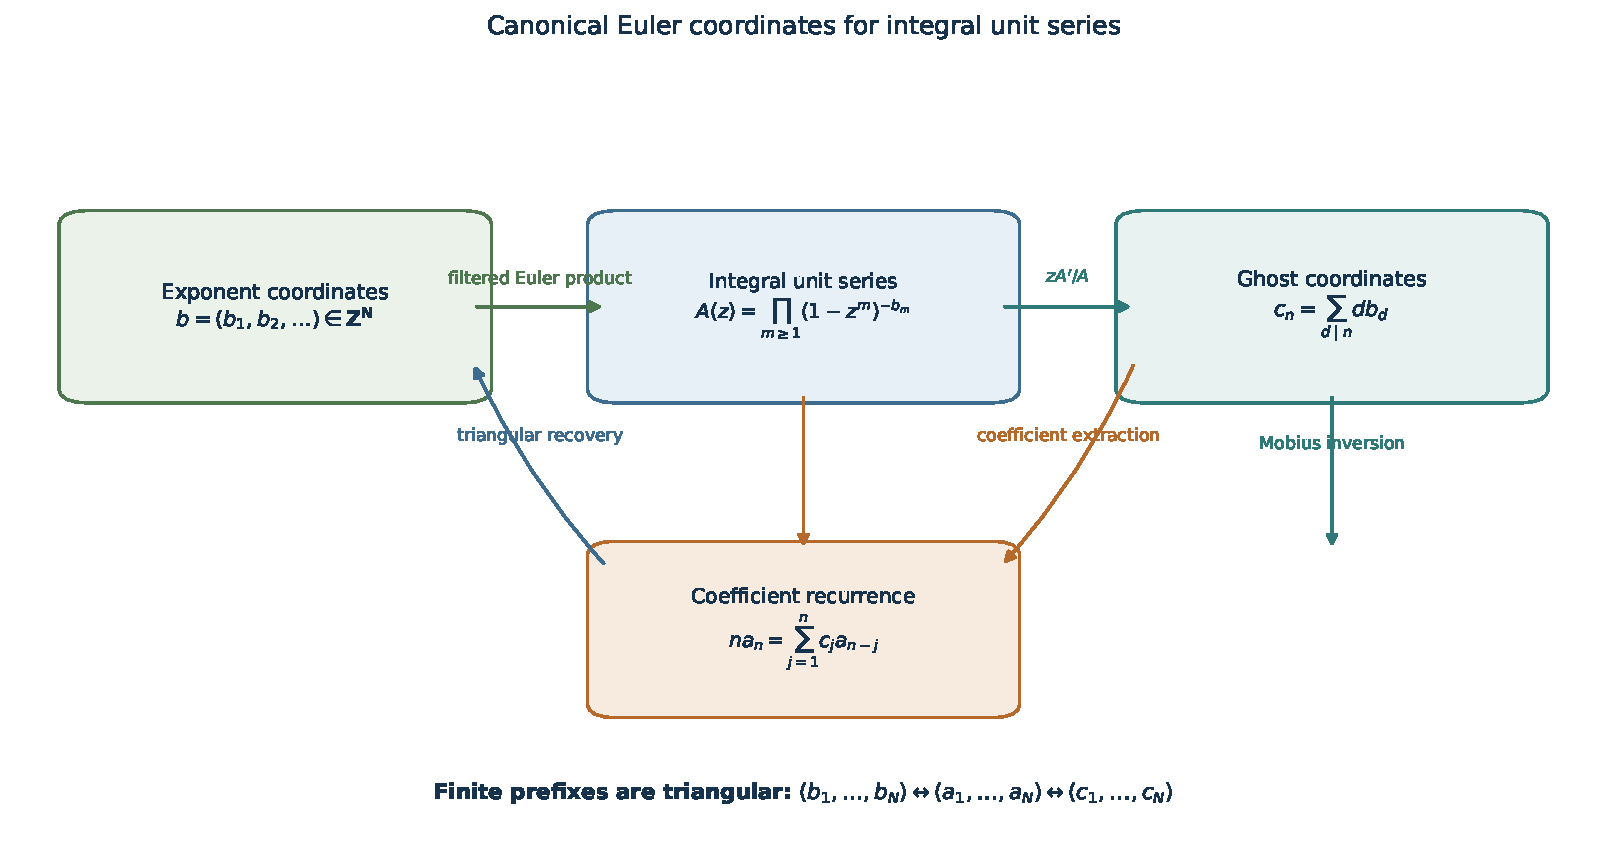
\includegraphics[width=0.99\textwidth]{euler_coordinate_atlas.pdf}
\caption{The fixed Euler basis gives three exact coordinate charts: integral exponents, coefficients, and divisor ghosts.  Every finite prefix is triangular, while the ghost chart is restricted by its explicit M\"obius divisibility conditions.}
\label{fig:block07-euler-atlas}
\end{figure}

\begin{example}[Partition and power families]
The following fixed-basis exponent functions give familiar filtered products:
\[
\begin{array}{c|c|c}
 b_n & A_b(z) & c_n\\
\hline
1 & \displaystyle\prod_{n\geq1}(1-z^n)^{-1} & \sigma_1(n)\\[4pt]
n & \displaystyle\prod_{n\geq1}(1-z^n)^{-n} & \sigma_2(n)\\[4pt]
n^r & \displaystyle\prod_{n\geq1}(1-z^n)^{-n^r} & \sigma_{r+1}(n).
\end{array}
\]
The first row is the ordinary partition series, and the second is the plane-partition series.  More generally, the power family converts the exponent rule $n^r$ into the divisor-sum ghost $\sigma_{r+1}$.
\end{example}

\begin{example}[Distinct parts and normalization]
The product
\[
\prod_{m\geq1}(1+z^m)
=
\prod_{m\geq1}\frac{1-z^{2m}}{1-z^m}
\]
has normalized Euler exponent
\[
b_n=
\begin{cases}
1,&n\text{ odd},\\
0,&n\text{ even}.
\end{cases}
\]
Thus the distinct-part and odd-part products become the same object after normalization in the fixed Euler basis.  This is an exact equality inside the declared product grammar, not a claim that arbitrary product grammars possess one preferred factorization.
\end{example}

\begin{boundary}[Coordinate universality versus compact structural realization]
\label{bnd:block07-storage-universality}
Theorem~\ref{thm:block07-euler-classification} gives a unique coordinate sequence for every integral unit series.  It does not make every such series finitely describable.  If the exponent sequence is merely an arbitrary list encoding all coefficients, the representation is storage universality.  A compact seed grammar additionally requires an effective finite rule for the exponent sequence or factor family.
\end{boundary}

\subsection{Multiplicative arithmetic functions as prime-power descent}

For arithmetic functions $f,g:\mathbb N_{\geq1}\to\mathbb Z$, write
\[
(f\mathbin{\ast_D}g)(n)
=
\sum_{d\mid n}f(d)g(n/d)
\]
for Dirichlet convolution.  Its identity is $\varepsilon(1)=1$ and $\varepsilon(n)=0$ for $n>1$.

\begin{definition}[Integral multiplicative category]
Let $\mathbf{Mult}_{\mathbb Z}$ be the discrete category whose objects are multiplicative arithmetic functions $f:\mathbb N_{\geq1}\to\mathbb Z$ satisfying
\[
f(1)=1,
\qquad
f(mn)=f(m)f(n)
\quad\text{when }(m,n)=1.
\]
The monoidal operation is Dirichlet convolution.
\end{definition}

\begin{proposition}[Dirichlet inverse and multiplicative closure]
If $f(1)=1$, then $f$ has a unique integral Dirichlet inverse.  If $f$ and $g$ are multiplicative, then $f\mathbin{\ast_D}g$ and $f^{-1_D}$ are multiplicative.
\end{proposition}

\begin{proof}
The coefficient equation at $n$ is triangular:
\[
g(1)=1,
\qquad
g(n)=-\sum_{\substack{d\mid n\\d<n}}f(n/d)g(d).
\]
Hence the inverse exists integrally and uniquely.  The standard coprime-divisor factorization of a divisor of $mn$ proves closure of multiplicative functions under convolution; uniqueness of the inverse then proves multiplicativity of $f^{-1_D}$.
\end{proof}

\begin{definition}[Prime-power seed series]
For a multiplicative function $f$ and a prime $p$, define
\[
F_{f,p}(T)
=
\sum_{e\geq0}f(p^e)T^e
\in1+T\mathbb Z[[T]].
\]
\end{definition}

\begin{theorem}[Prime-power descent equivalence]
\label{thm:block07-prime-power-descent}
The assignment
\[
f\longmapsto\bigl(F_{f,p}\bigr)_p
\]
is a group isomorphism
\[
\boxed{
(\mathbf{Mult}_{\mathbb Z},\mathbin{\ast_D})
\simeq
\prod_{p\text{ prime}}
(1+T\mathbb Z[[T]],\cdot).
}
\]
The inverse reconstructs
\[
\boxed{
f(n)=\prod_{p^e\parallel n}f(p^e).}
\]
Under this correspondence,
\[
F_{f\ast_D g,p}(T)
=
F_{f,p}(T)F_{g,p}(T).
\]
\end{theorem}

\begin{proof}
Unique factorization writes every positive integer as a finite product of pairwise coprime prime powers, so multiplicativity gives the reconstruction formula.  Conversely, an arbitrary family of local unit series defines a multiplicative function by the same finite product.  For $n=p^e$, Dirichlet convolution becomes
\[
(f\mathbin{\ast_D}g)(p^e)
=
\sum_{r=0}^{e}f(p^r)g(p^{e-r}),
\]
which is exactly the coefficient of $T^e$ in the local Cauchy product.
\end{proof}

\subsection{Prime-Euler and local ghost coordinates}

Apply the Euler-coordinate theorem independently at each prime:
\[
F_{f,p}(T)
=
\prod_{m\geq1}(1-T^m)^{-\beta_{p,m}(f)}.
\]
Define local ghosts
\[
\gamma_{p,e}(f)
=
\sum_{d\mid e}d\,\beta_{p,d}(f).
\]

\begin{theorem}[Complete prime-Euler coordinates]
\label{thm:block07-prime-euler}
For integral multiplicative functions, the following normalized data are equivalent and complete:
\[
 f,
\qquad
\bigl(F_{f,p}\bigr)_p,
\qquad
\bigl(\beta_{p,m}(f)\bigr)_{p,m},
\qquad
\bigl(\gamma_{p,e}(f)\bigr)_{p,e}.
\]
Dirichlet convolution is linearized by the last two charts:
\[
\beta_{p,m}(f\mathbin{\ast_D}g)
=
\beta_{p,m}(f)+\beta_{p,m}(g),
\]
\[
\gamma_{p,e}(f\mathbin{\ast_D}g)
=
\gamma_{p,e}(f)+\gamma_{p,e}(g).
\]
The ghost chart consists exactly of the prime-indexed sequences satisfying the local M\"obius divisibility conditions
\[
\frac1e\sum_{d\mid e}\mu\!\left(\frac ed\right)\gamma_{p,d}\in\mathbb Z.
\]
\end{theorem}

\begin{proof}
Theorem~\ref{thm:block07-euler-classification} and Theorem~\ref{thm:block07-ghost-equivalence} apply to each local unit series $F_{f,p}$.  The prime-power descent theorem then reconstructs the global function.  Local multiplication corresponds to Dirichlet convolution, while Euler exponents and ghosts add under multiplication.
\end{proof}

\begin{theorem}[Valuation logarithmic derivative]
\label{thm:block07-valuation-derivative}
Fix a prime $p$.  Let $\Gamma_{f,p}$ be the arithmetic function supported on powers of $p$ with
\[
\Gamma_{f,p}(1)=0,
\qquad
\Gamma_{f,p}(p^e)=\gamma_{p,e}(f)
\quad(e\geq1).
\]
Then
\[
\boxed{
(v_p\cdot f)(n)
=
(\Gamma_{f,p}\mathbin{\ast_D}f)(n)
\qquad(n\geq1).
}
\]
Equivalently,
\[
\frac{T F_{f,p}'(T)}{F_{f,p}(T)}
=
\sum_{e\geq1}\gamma_{p,e}(f)T^e.
\]
\end{theorem}

\begin{proof}
The local logarithmic-derivative recurrence gives
\[
e f(p^e)
=
\sum_{j=1}^{e}\gamma_{p,j}(f)f(p^{e-j}).
\]
Write $n=p^e u$ with $(u,p)=1$ and multiply by $f(u)$.  Since $\Gamma_{f,p}$ is supported on $p$-powers, the resulting sum is exactly the Dirichlet convolution at $n$.
\end{proof}

\begin{proposition}[Multiplicative residue-packet law]
For $N\geq1$, let $P_{N,r}f$ be the arithmetic function equal to $f(n)$ when $n\equiv r\pmod N$ and zero otherwise.  Then
\[
\boxed{
P_{N,k}(f\mathbin{\ast_D}g)
=
\sum_{rs\equiv k\, (N)}
(P_{N,r}f)\mathbin{\ast_D}(P_{N,s}g).
}
\]
Thus the packet address algebra for Dirichlet convolution is the finite multiplicative monoid $\mathbb Z/N\mathbb Z$, including its zero divisors.
\end{proposition}

\begin{proof}
In each divisor pair $n=d(n/d)$, the residue of $n$ modulo $N$ is the product of the two divisor residues.  Group the divisor sum by those two residues.
\end{proof}

\begin{figure}[htbp]
\centering
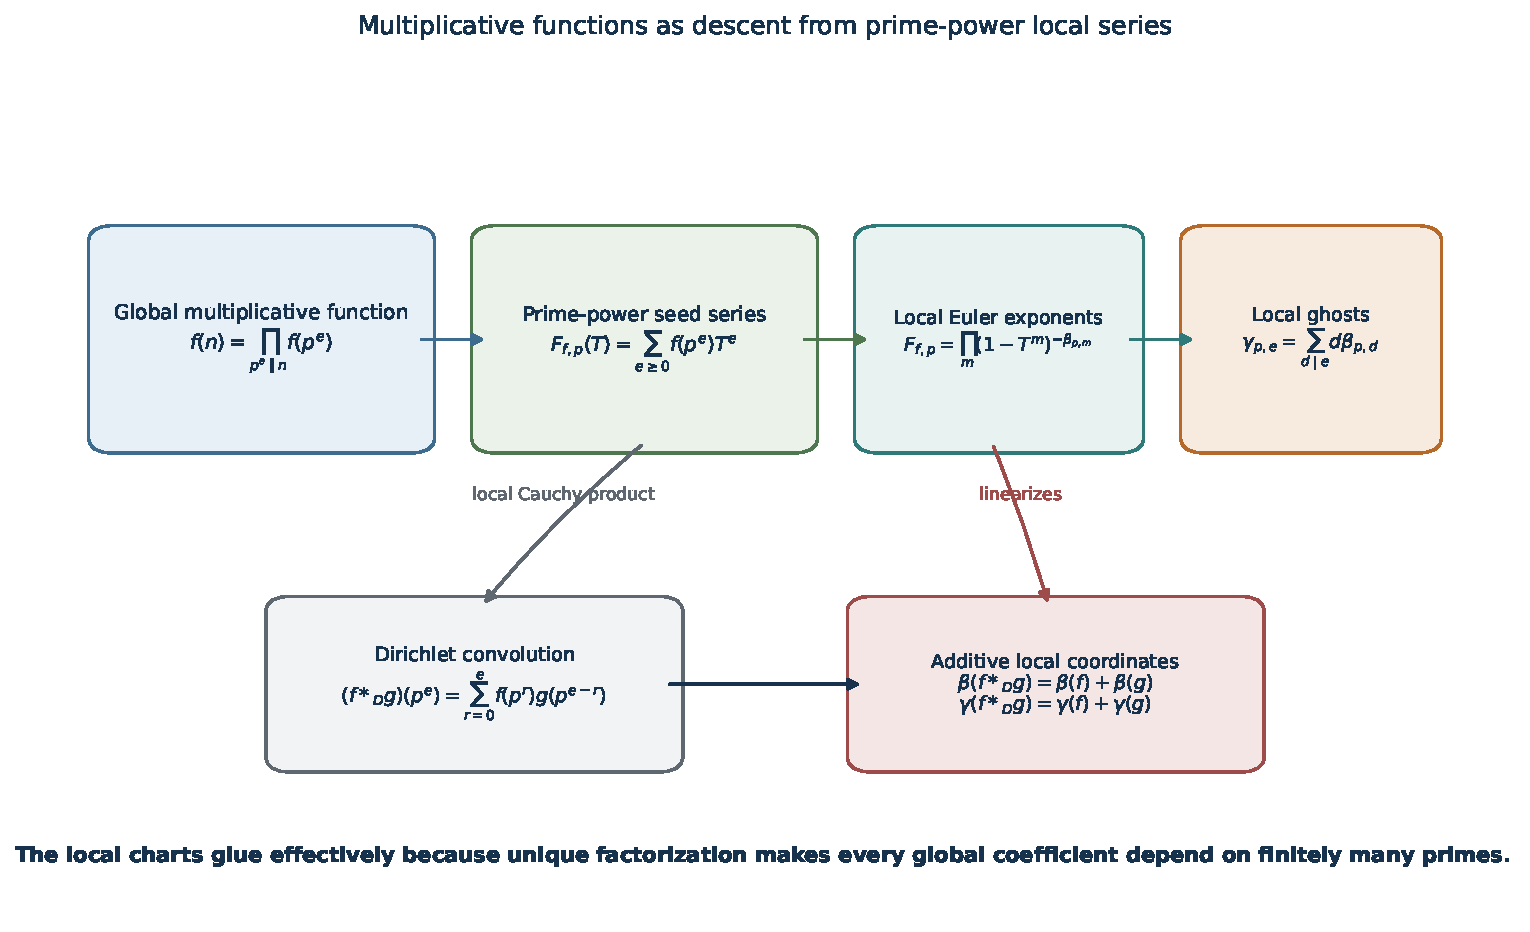
\includegraphics[width=0.99\textwidth]{multiplicative_prime_power_atlas.pdf}
\caption{A multiplicative arithmetic function is effective descent data over its prime-power local series.  Local Euler exponents and local ghosts turn Dirichlet convolution into addition.}
\label{fig:block07-multiplicative-atlas}
\end{figure}

\begin{table}[htbp]
\centering
\caption{Named prime-power seed families in local Euler coordinates.}
\label{tab:block07-named-local}
\scriptsize
\begin{tabularx}{\textwidth}{@{}L{0.24\textwidth}L{0.23\textwidth}L{0.25\textwidth}Y@{}}
\toprule
Arithmetic function & Nonzero local Euler exponents & Prime-power seed & Local ghost\\
\midrule
Constant-one function $\mathbf 1$ & $\beta_{1}=1$ & $1,1,1,1,1,1,\ldots$ & $1,1,1,1,1,1,\ldots$\\
M\"obius $\mu$ & $\beta_{1}=-1$ & $1,-1,0,0,0,0,\ldots$ & $-1,-1,-1,-1,-1,-1,\ldots$\\
Liouville $\lambda$ & $\beta_{1}=-1$, $\beta_{2}=1$ & $1,-1,1,-1,1,-1,\ldots$ & $-1,1,-1,1,-1,1,\ldots$\\
Squarefree indicator $\mu^2$ & $\beta_{1}=1$, $\beta_{2}=-1$ & $1,1,0,0,0,0,\ldots$ & $1,-1,1,-1,1,-1,\ldots$\\
Three-fold divisor function $\tau_3$ & $\beta_{1}=3$ & $1,3,6,10,15,21,\ldots$ & $3,3,3,3,3,3,\ldots$\\
\bottomrule
\end{tabularx}
\end{table}


\subsection{The divisor--ghost cross-stratum bridge}

The Euler ghost transform can itself be written in the Dirichlet-convolution language.  Let $\mathbf{1}(n)=1$, let $\operatorname{id}(n)=n$, and let pointwise multiplication be denoted by a centered dot.

\begin{definition}[Divisor--ghost transform]
For an arithmetic exponent function $b:\mathbb N_{\geq1}\to\mathbb Z$, define
\[
\mathfrak G(b)
=
\mathbf{1}\mathbin{\ast_D}(\operatorname{id}\cdot b),
\]
so that
\[
\mathfrak G(b)(n)
=
\sum_{d\mid n}d\,b(d).
\]
\end{definition}

\begin{theorem}[Exact divisor--ghost bridge]
\label{thm:block07-divisor-ghost}
The map $b\mapsto c=\mathfrak G(b)$ is injective, with inverse
\[
\boxed{
b(n)
=
\frac1n
(\mu\mathbin{\ast_D}c)(n).
}
\]
Its integral image consists exactly of the arithmetic functions $c$ satisfying
\[
n\mid(\mu\mathbin{\ast_D}c)(n)
\qquad(n\geq1).
\]
For the Euler product
\[
A_b(z)=\prod_{n\geq1}(1-z^n)^{-b(n)},
\]
one has
\[
\frac{zA_b'(z)}{A_b(z)}
=
\sum_{n\geq1}c(n)z^n.
\]
\end{theorem}

\begin{proof}
The first identity is the convolution form of the divisor sum.  Since $\mu\mathbin{\ast_D}\mathbf{1}=\varepsilon$,
\[
\mu\mathbin{\ast_D}c
=
\operatorname{id}\cdot b.
\]
Division by $n$ gives the inverse and its exact integrality condition.  The logarithmic-derivative identity is Theorem~\ref{thm:block07-ghost-equivalence} with the exponent sequence regarded as an arithmetic function.
\end{proof}

\begin{theorem}[Multiplicativity is preserved and reflected]
\label{thm:block07-multiplicative-ghost}
Assume $b(1)=1$ and $c=\mathfrak G(b)$.  Then
\[
\boxed{
b\text{ is multiplicative}
\quad\Longleftrightarrow\quad
c\text{ is multiplicative}.}
\]
On this locus, both $b$ and $c$ are reconstructed from prime-power seeds.  For every prime $p$ and $e\geq1$,
\[
\boxed{
c(p^e)=\sum_{j=0}^{e}p^j b(p^j),}
\]
\[
\boxed{
b(p^e)=\frac{c(p^e)-c(p^{e-1})}{p^e}.}
\]
\end{theorem}

\begin{proof}
If $b$ is multiplicative, then $\operatorname{id}\cdot b$ is multiplicative, and Dirichlet convolution with $\mathbf{1}$ preserves multiplicativity.  Conversely, if $c$ is multiplicative, then $\mu\mathbin{\ast_D}c$ is multiplicative.  Dividing pointwise by the completely multiplicative function $\operatorname{id}$ preserves multiplicativity over $\mathbb Q$; the integral image condition ensures that the resulting values are integers.  The prime-power formulas follow by listing the divisors of $p^e$ and subtracting consecutive sums.
\end{proof}

\begin{figure}[htbp]
\centering
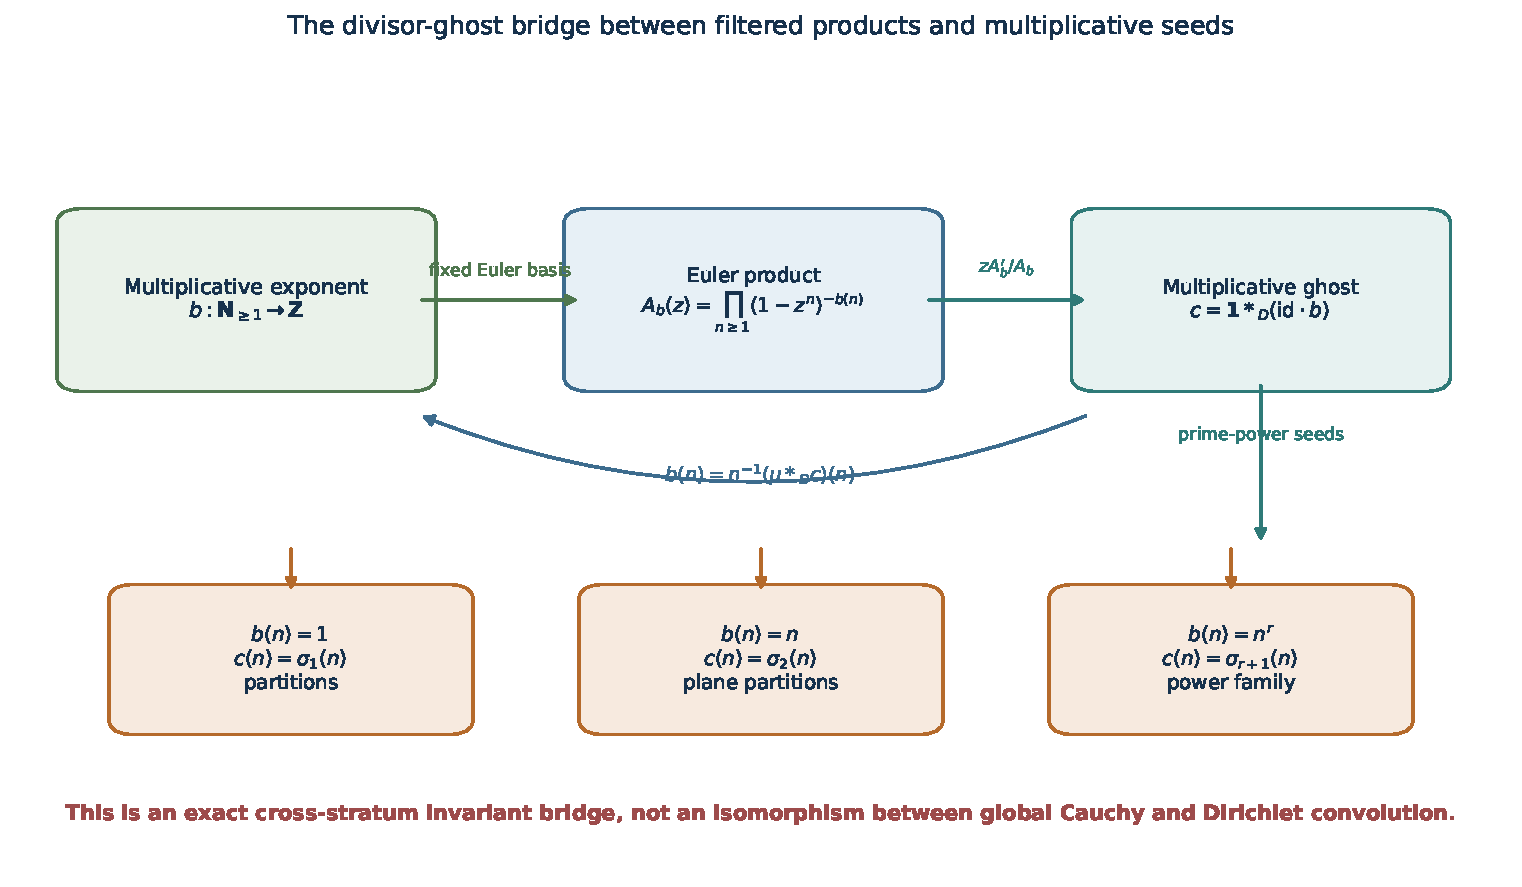
\includegraphics[width=0.99\textwidth]{divisor_ghost_bridge.pdf}
\caption{The divisor--ghost transform gives a reversible invariant bridge on the multiplicative exponent locus.  It connects a fixed-basis ordinary Euler product to multiplicative prime-power data without identifying the two global convolution algebras.}
\label{fig:block07-divisor-ghost}
\end{figure}

\subsection{A restricted product--multiplicative atlas}

\begin{definition}[Multiplicative Euler-overlap category]
Let $\mathbf{EulMult}_{\mathbb Z}$ be the discrete category of multiplicative exponent functions
\[
b:\mathbb N_{\geq1}\to\mathbb Z,
\qquad b(1)=1.
\]
Associate to $b$ the four normalized charts
\[
\mathsf B(b)=b,
\qquad
\mathsf A(b)=A_b(z),
\qquad
\mathsf C(b)=\mathfrak G(b),
\qquad
\mathsf P(b)=\bigl(b(p^e),c(p^e)\bigr)_{p,e}.
\]
\end{definition}

\begin{theorem}[Effective descent on the divisor--ghost overlap]
\label{thm:block07-product-multiplicative-descent}
The exponent, fixed Euler-product, multiplicative ghost, and prime-power seed charts form a finite normalized atlas
\[
\mathfrak R_{\mathrm{DG}}.
\]
Every bridge is reversible on the declared overlap, every multiple-overlap comparison is the unique identity over the represented exponent function, and
\[
\boxed{
\Desc(\mathfrak R_{\mathrm{DG}})
\simeq
\mathbf{EulMult}_{\mathbb Z}.
}
\]
Descent is effective for objects and morphisms.
\end{theorem}

\begin{proof}
The Euler-product chart is uniquely inverted by Theorem~\ref{thm:block07-euler-classification}.  The ghost chart is uniquely inverted by Theorem~\ref{thm:block07-divisor-ghost}.  The prime-power chart is uniquely inverted by multiplicativity and unique factorization.  Hence every normalized fiber over $b$ is a singleton.  All comparison cells and all multiple-overlap coherence laws are therefore forced to be identities.  A compatible local family glues to its common exponent function, and morphism effectivity is automatic because the chart categories are discrete.
\end{proof}

\begin{theorem}[Complete descended prime-power invariant]
\label{thm:block07-complete-product-invariant}
The prime-power package
\[
\boxed{
\mathcal J_{\mathrm{DG}}(b)
=
\left(
 b(p^e),
 c(p^e)
\right)_{p\text{ prime},\ e\geq0}
}
\]
subject to
\[
p^e b(p^e)=c(p^e)-c(p^{e-1})
\quad(e\geq1)
\]
is complete on $\mathbf{EulMult}_{\mathbb Z}$.  It reconstructs $b$, $c$, the Euler product $A_b$, and the coefficient recurrence of $A_b$.
\end{theorem}

\begin{proof}
Prime-power values reconstruct the multiplicative functions $b$ and $c$.  Theorem~\ref{thm:block07-euler-classification} reconstructs $A_b$, and Theorem~\ref{thm:block07-euler-recurrence} reconstructs its coefficient sequence from $c$.  Therefore equal invariant packages imply equality in every chart.
\end{proof}

\begin{example}[Power bridge]
For $b(n)=n^r$, which is completely multiplicative, the divisor ghost is
\[
c(n)=\sum_{d\mid n}d^{r+1}=\sigma_{r+1}(n).
\]
At a prime power,
\[
\sigma_{r+1}(p^e)
=
1+p^{r+1}+\cdots+p^{e(r+1)}.
\]
Thus one simple multiplicative exponent rule simultaneously produces a filtered ordinary product, a multiplicative divisor-sum ghost, and a one-dimensional geometric local rule at every prime.
\end{example}

\subsection{Why the bridge is restricted}

\begin{proposition}[The multiplicative exponent locus is not a product subgroup]
The set of multiplicative Euler exponent functions is not closed under the addition of exponent coordinates.  Consequently, multiplication of the corresponding ordinary Euler products does not define an internal group law on $\mathbf{EulMult}_{\mathbb Z}$.
\end{proposition}

\begin{proof}
The constant function $b(n)=1$ is multiplicative.  But $b+b$ has value $2$ at $1$ and therefore is not multiplicative under the normalization $f(1)=1$.  Since ordinary Euler-product multiplication adds exponents, the multiplicative exponent locus is not closed under that operation.
\end{proof}

\begin{proposition}[Euler coefficients are not multiplicative semantics]
The coefficient sequence of $A_b(z)$ need not be a multiplicative arithmetic function even when $b$ is multiplicative.  For example, $b(n)=1$ gives the partition numbers, and
\[
p(6)=11\neq p(2)p(3)=6.
\]
\end{proposition}

\begin{boundary}[Prime-power data require multiplicativity]
Two arbitrary arithmetic functions can agree on every prime power and differ on a composite supported at more than one prime.  Prime-power seeds are complete only after the multiplicativity axiom has been declared.  A compact local seed rule also does not remove the computational cost of factoring the input integer.
\end{boundary}

\begin{figure}[htbp]
\centering
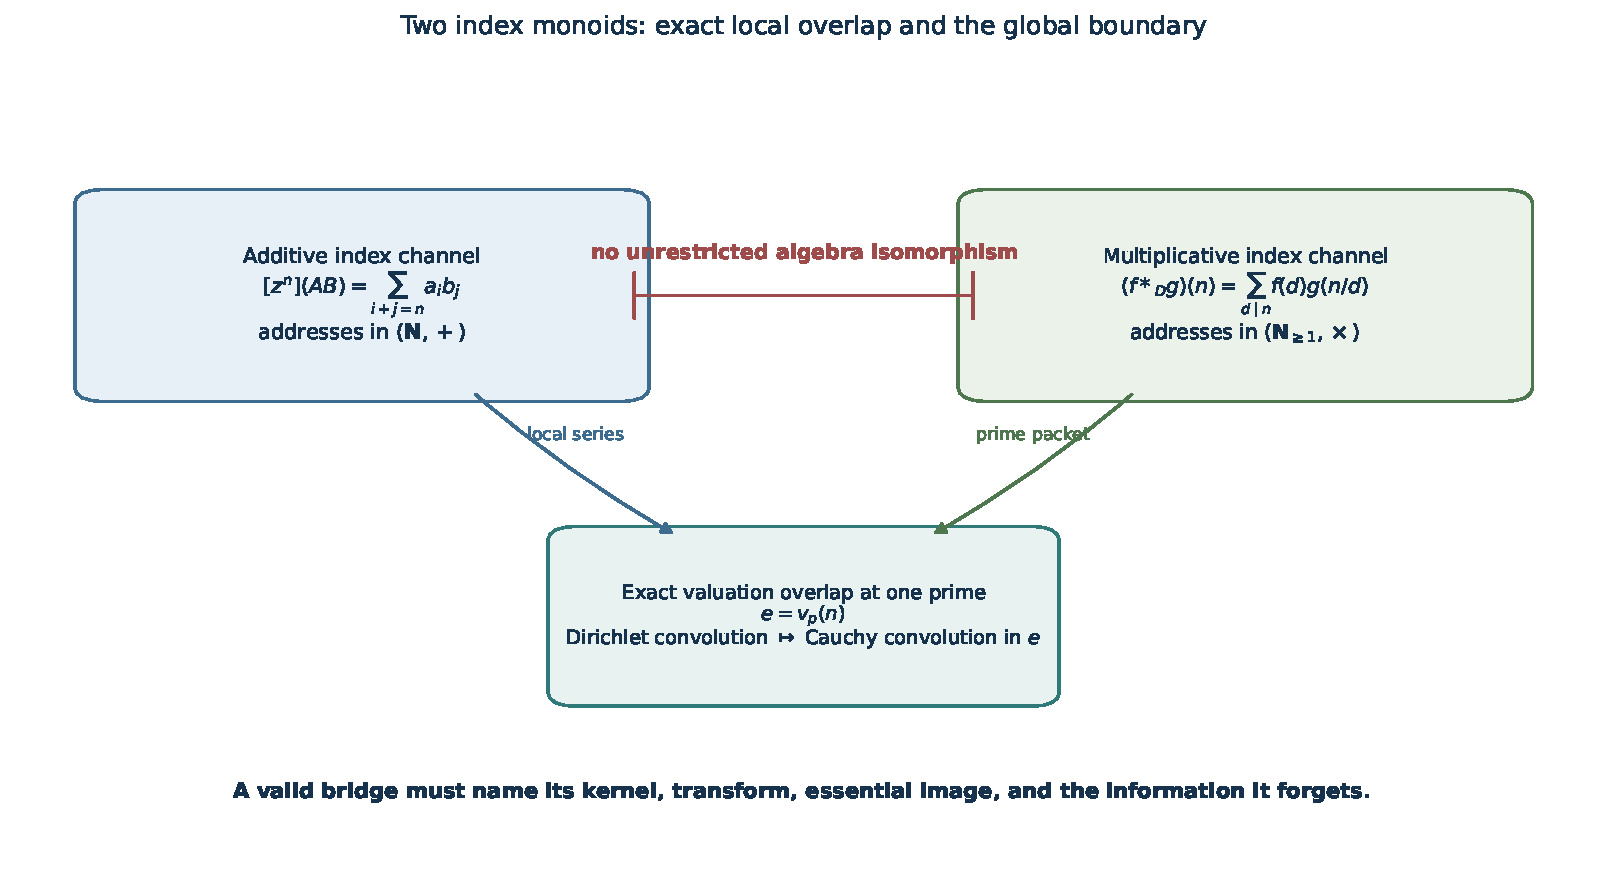
\includegraphics[width=0.98\textwidth]{two_monoid_boundary.pdf}
\caption{Cauchy and Dirichlet convolution use different global address monoids.  They overlap exactly after localization at one valuation coordinate, but no unrestricted algebra equivalence follows.}
\label{fig:block07-two-monoids}
\end{figure}

\begin{boundary}[No universal additive--multiplicative equivalence]
\label{bnd:block07-no-global-convolution-equivalence}
The divisor--ghost transform is an exact invariant bridge on a named essential image.  It is not an algebra isomorphism between ordinary Cauchy convolution and Dirichlet convolution, does not identify the coefficients of an Euler product with a multiplicative function, and does not produce a canonical factorization across arbitrary product grammars.  Any larger bridge must name its transform, kernel, essential image, and information-loss profile.
\end{boundary}

\subsection{Exact finite verification}

\begin{table}[htbp]
\centering
\caption{Exact finite validation of the Product-multiplicative atlas filtered-product and multiplicative layer.}
\label{tab:block07-validation}
\small
\begin{tabularx}{\textwidth}{@{}L{0.31\textwidth}Y@{}}
\toprule
Check family & Recorded result\\
\midrule
Euler-coordinate atlas & 15625 exponent prefixes and 3125 arbitrary integral unit-series prefixes.\\
Prime-power multiplicative atlas & 96 deterministic local systems and 48 Dirichlet-convolution pairs.\\
Divisor-ghost overlap & 128 multiplicative exponent systems and 6 power families.\\
Named local coordinates & 5 arithmetic families and 6 geometric necklace modes.\\
Total exact checks & 595964; 0 failures.\\
Overall status & PASS.\\
Boundary & Bounded exact verification supports the printed formulas and examples. It does not establish compactness or minimality for arbitrary product grammars, nor a global Cauchy--Dirichlet algebra isomorphism.\\
\bottomrule
\end{tabularx}
\end{table}


The Product-multiplicative atlas verifier performs four exact audits.  First, it exhaustively checks the coefficient, exponent, and ghost triangular maps for every exponent prefix in $\{-2,-1,0,1,2\}^6$ and every unit coefficient prefix in $\{-2,-1,0,1,2\}^5$.  Second, it constructs deterministic prime-power systems, reconstructs global multiplicative functions, and verifies local Euler inversion, local logarithmic derivatives, and Dirichlet convolution.  Third, it checks the divisor--ghost bridge and the power family $b(n)=n^r$.  Fourth, it verifies the named local Euler coordinates printed in \cref{tab:block07-named-local}.  The recorded 595,964 exact checks have no failures.

\begin{boundarybox}
\textbf{Exact boundary of Product-multiplicative atlas.}
The fixed Euler basis gives a canonical coordinate system for integral unit series, and prime-power seed series give a canonical coordinate system for integral multiplicative functions.  The divisor--ghost transform produces one complete cross-stratum overlap on multiplicative exponent functions.  The block does not prove compactness for arbitrary exponent data, a minimal product compiler, closure of the multiplicative exponent slice under ordinary product multiplication, a global Cauchy--Dirichlet algebra isomorphism, or a canonical factorization across unrestricted product grammars.
\end{boundarybox}

\begin{resultbox}
\textbf{Section result.}
Integral unit series admit unique fixed-basis Euler exponents and unique divisor ghosts, with exact logarithmic-derivative recurrence and finite-prefix triangularity.  Integral multiplicative functions are effective descent from prime-power local series; local Euler exponents and local ghosts linearize Dirichlet convolution and form complete invariants.  On the multiplicative exponent locus, the divisor--ghost transform gives a reversible four-chart atlas linking exponent functions, ordinary filtered Euler products, multiplicative ghosts, and prime-power seeds.  This closes one explicit product--multiplicative invariant bridge while preserving the global distinction between additive and multiplicative index monoids.
\end{resultbox}



\section{Local Newton--Mahler coordinates, affine polyphase descent, and precision ladders}
\label{sec:block08-local}

Local Mahler-polyphase atlas develops the local stratum promised by the work program.  Its purpose is not to merge every use of the word ``Mahler.''  It freezes one precise local semantic doctrine, constructs its normalized coefficient and polyphase charts, types the characteristic-zero, integral, and residue-level affine channels separately, and identifies the exact data needed to pass from finite modular dynamics to certified local analytic packets.

\subsection{Two Mahler languages and the declared local doctrine}
\label{subsec:block08-two-languages}

Two constructions in the Library use the same historical name but have different variables and different semantics.

\begin{enumerate}
\item A \emph{functional-Mahler equation}
\[
 F(z)=R(z)F(z^p)
\]
is an identity for a formal coefficient series in the variable \(z\).  Cartier operators act on the coefficient index.  the periodic and rational-mask atlases use this channel over finite fields.
\item A \emph{Newton--Mahler expansion}
\[
 f(x)=\sum_{r\geq0}c_r\binom xr
\]
is a coordinate expansion for a function of a \(p\)-adic input variable \(x\).  Affine substitutions \(x=Mq+s\) produce polyphase branches of the input domain.
\end{enumerate}

This section treats the second channel.  Fix a prime \(p\).  Let
\[
 \mathcal C_p=C(\mathbb Z_p,\mathbb Z_p)
\]
with the uniform norm, and let
\[
 c_0(\mathbb Z_p)
 =
 \left\{c=(c_r)_{r\geq0}:c_r\in\mathbb Z_p,\ c_r\longrightarrow0\right\}
\]
with the coefficient sup norm.

\begin{theorem}[Mahler coordinate theorem]
\label{thm:block08-mahler-coordinate}
The synthesis map
\[
 \mathcal M_p:c_0(\mathbb Z_p)\longrightarrow\mathcal C_p,
 \qquad
 c\longmapsto
 \left(x\longmapsto\sum_{r\geq0}c_r\binom xr\right),
\]
is an isometric isomorphism of \(\mathbb Z_p\)-modules.  Its inverse is
\[
 \boxed{c_r=\Delta^r f(0).}
\]
In particular, the Newton--Mahler coefficient sequence is a canonical complete coordinate for a continuous \(\mathbb Z_p\)-valued function.
\end{theorem}

\begin{proof}
This is the classical Mahler coordinate theorem \cite{Mahler1958}.  Finite Newton interpolation gives the coefficient identity on nonnegative integers.  Continuity implies that the forward-difference coefficients tend to zero, so the binomial series converges uniformly on \(\mathbb Z_p\).  Conversely, every coefficient sequence tending to zero gives a uniformly convergent continuous function.  Uniqueness follows from the finite-difference formula.
\end{proof}

\begin{definition}[Exact valuation profile and certified class]
\label{def:block08-weight-class}
For \(f=\mathcal M_p(c)\), define
\[
 \nu_f(r)=v_p(c_r)\in\mathbb Z_{\geq0}\cup\{\infty\}.
\]
If \(w:\mathbb N\to\mathbb Z_{\geq0}\) is nondecreasing and tends to infinity, put
\[
 \mathcal M_w
 =
 \{c\in c_0(\mathbb Z_p):v_p(c_r)\geq w(r)\},
 \qquad
 \mathcal C_w=\mathcal M_p(\mathcal M_w).
\]
The function \(w\) is a declared precision certificate.  The class \(\mathcal C_w\) is not asserted to be a characterization of every possible notion of local analyticity.
\end{definition}

\begin{figure}[htbp]
\centering
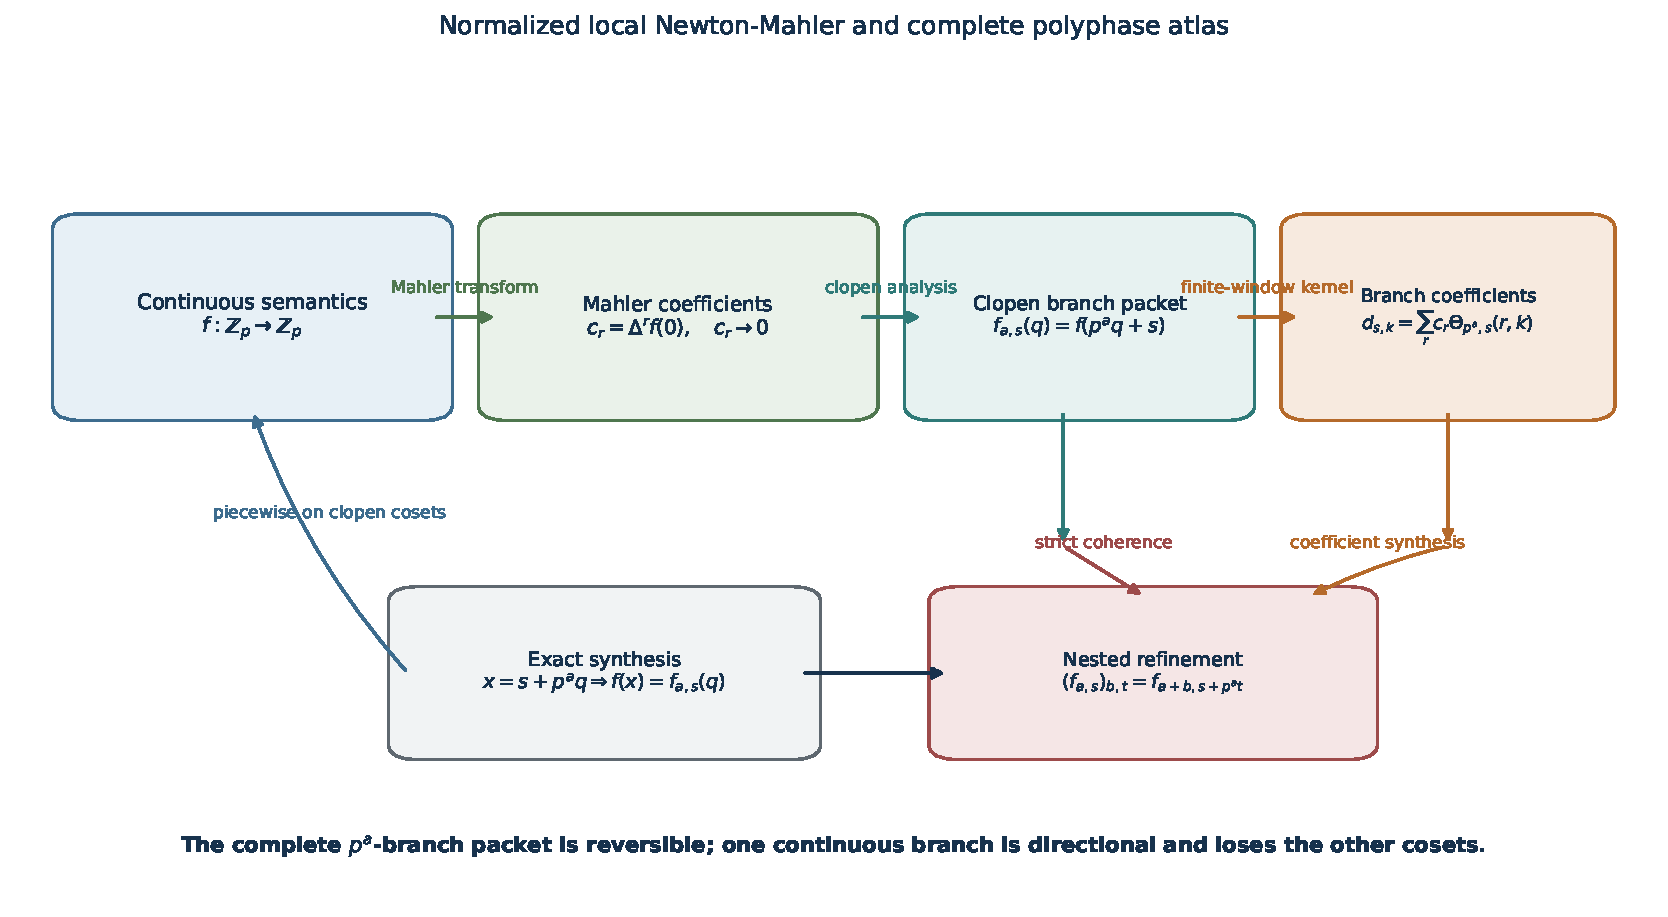
\includegraphics[width=.98\textwidth]{local_mahler_atlas.pdf}
\caption{The normalized local atlas.  Continuous semantics, canonical Mahler coefficients, complete clopen branch packets, and branchwise Mahler coefficients are equivalent charts.  A single continuous branch remains directional.}
\label{fig:block08-local-atlas}
\end{figure}

\subsection{Complete clopen packets and effective local descent}
\label{subsec:block08-clopen-descent}

For \(a\geq1\) and \(0\leq s<p^a\), define the branch
\[
 \mathcal B_{a,s}f(q)=f(p^a q+s),
 \qquad q\in\mathbb Z_p,
\]
and the complete packet
\[
 \mathcal B_a f=\bigl(\mathcal B_{a,s}f\bigr)_{0\leq s<p^a}.
\]

\begin{theorem}[Complete clopen packet equivalence]
\label{thm:block08-clopen-equivalence}
The analysis map
\[
 \mathcal B_a:\mathcal C_p
 \longrightarrow
 \prod_{s=0}^{p^a-1}\mathcal C_p
\]
is an isometric isomorphism.  Its inverse is the piecewise synthesis
\[
 \boxed{
 (\mathcal S_a g)(x)
 =g_s\!\left(\frac{x-s}{p^a}\right)
 \quad\text{for }x\in s+p^a\mathbb Z_p.}
\]
Thus the clopen residue cover of \(\mathbb Z_p\) has effective descent for both objects and equality morphisms.
\end{theorem}

\begin{proof}
The cosets \(s+p^a\mathbb Z_p\) are pairwise disjoint, clopen, and cover \(\mathbb Z_p\).  Restriction followed by the displayed synthesis is the identity.  Conversely, synthesis followed by restriction recovers every component.  Continuity is checked separately on each clopen component, and the uniform norm is the maximum of the branch norms.
\end{proof}

\begin{theorem}[Strict nested-branch law]
\label{thm:block08-nested-branches}
For \(a,b\geq1\), \(0\leq s<p^a\), and \(0\leq t<p^b\),
\[
 \boxed{(f_{a,s})_{b,t}=f_{a+b,s+p^a t}.}
\]
All multiple-overlap comparison cells for the nested \(p\)-power branch atlas are identities.  Hence its higher coherence is strict rather than merely up to a chosen natural isomorphism.
\end{theorem}

\begin{proof}
Direct substitution gives
\[
 f_{a,s}(p^bq+t)
 =f(p^a(p^bq+t)+s)
 =f(p^{a+b}q+s+p^a t).
\]
The address is uniquely determined in the interval \(0\leq s+p^a t<p^{a+b}\).
\end{proof}

A single branch \(\mathcal B_{a,s}\) is not injective on \(\mathcal C_p\) when \(a\geq1\): any nonzero continuous function supported on another clopen coset lies in its kernel.  The complete packet is therefore the reversible object.  This observation will be contrasted below with the finite-degree characteristic-zero polynomial chart, where one affine branch is invertible.

\subsection{The affine Mahler kernel and mixed-radix coherence}
\label{subsec:block08-affine-kernel}

For \(M\geq1\), \(s\geq0\), and \(r,k\geq0\), define
\[
 \Phi_M(z)=(1+z)^M-1
\]
and
\[
 \boxed{
 \Theta_{M,s}(r,k)
 =[z^r](1+z)^s\Phi_M(z)^k.}
\]
Equivalently,
\[
 \boxed{
 \Theta_{M,s}(r,k)
 =\sum_{j=0}^{k}(-1)^{k-j}\binom kj\binom{Mj+s}{r}.}
\]
The support is finite:
\[
 \Theta_{M,s}(r,k)=0
 \quad\text{unless}\quad
 k\leq r\leq Mk+s.
\]

\begin{theorem}[Affine Newton--Mahler transfer]
\label{thm:block08-affine-transfer}
Let
\[
 f(x)=\sum_{r\geq0}c_r\binom xr
\]
be a convergent Mahler expansion and put \(g_s(q)=f(Mq+s)\).  Then
\[
 g_s(q)=\sum_{k\geq0}d_{s,k}\binom qk,
\]
where
\[
 \boxed{
 d_{s,k}
 =\sum_{r=k}^{Mk+s}c_r\Theta_{M,s}(r,k).}
\]
Every output coefficient depends on a finite source window.
\end{theorem}

\begin{proof}
Expand
\[
 (1+z)^{Mq+s}
 =(1+z)^s\bigl(1+\Phi_M(z)\bigr)^q
 =\sum_{k\geq0}\binom qk(1+z)^s\Phi_M(z)^k.
\]
Taking \([z^r]\) gives the affine expansion of \(\binom{Mq+s}{r}\).  Substitution into the Mahler series gives the formula.  The finite support of \(\Theta_{M,s}\) makes each coefficient sum finite.
\end{proof}

Let \(\mathcal T_{M,s}\) denote this coefficient operator.  Conjugating the clopen packet theorem by \(\mathcal M_p\) gives the following normalized coefficient atlas.

\begin{corollary}[Complete coefficient-packet equivalence]
\label{cor:block08-coefficient-packet}
For \(M=p^a\), the map
\[
 \mathcal T_a:c_0(\mathbb Z_p)
 \longrightarrow
 \prod_{s=0}^{p^a-1}c_0(\mathbb Z_p),
 \qquad
 c\longmapsto(\mathcal T_{p^a,s}c)_s,
\]
is a topological isomorphism.  It is the coefficient conjugate of complete clopen analysis.
\end{corollary}

\begin{theorem}[Mixed-radix kernel composition]
\label{thm:block08-kernel-composition}
For \(M,N\geq1\),
\[
 \boxed{
 \sum_{k\geq0}
 \Theta_{M,s}(r,k)\Theta_{N,t}(k,\ell)
 =
 \Theta_{MN,Mt+s}(r,\ell).}
\]
Equivalently,
\[
 \boxed{
 \mathcal T_{N,t}\mathcal T_{M,s}
 =
 \mathcal T_{MN,Mt+s}.}
\]
When \(\gcd(M,N)=1\), the two Chinese-remainder refinement paths to a common address agree exactly.  Their holonomy is the identity.
\end{theorem}

\begin{proof}
Apply the affine substitution \(x=Mq+s\), then \(q=Ny+t\).  The composite is \(x=MNy+Mt+s\).  Uniqueness of Mahler coefficients yields the kernel identity.  The Chinese-remainder diamond is the same equality written along two factorizations of one affine address.
\end{proof}

\begin{resultbox}
\textbf{Normalized local atlas.}
For every fixed prime \(p\) and depth \(a\), the following normalized charts are equivalent:
\[
 \boxed{
 \mathbf{Loc}^{\mathrm{cts}}_p
 \simeq
 \mathbf{Mah}^{c_0}_p
 \simeq
 \mathbf{Branch}^{\mathrm{cts}}_{p,a}
 \simeq
 \mathbf{BranchMah}^{c_0}_{p,a}.}
\]
The first chart contains continuous functions on \(\mathbb Z_p\), the second their unique Mahler coefficients, the third the complete clopen branch packet, and the fourth the corresponding branchwise coefficient packet.  Every normalized fiber is contractible.  The descent category is therefore equivalent to the discrete semantic category \(\mathbf{Loc}^{\mathrm{cts}}_p\).
\end{resultbox}

\subsection{Finite-degree bridge ladder and collective recovery}
\label{subsec:block08-finite-degree}

The same integer kernel matrix has different categorical status after changing the coefficient doctrine.  Fix \(d\geq0\) and write
\[
 \mathcal M_d(R)=R^{d+1}
\]
for the formal truncated Mahler coefficient module.  Let
\[
 A_{M,s}^{(d)}
 =\bigl[\Theta_{M,s}(r,k)\bigr]_{0\leq k,r\leq d},
\]
where the target degree \(k\) is the row index.

\begin{theorem}[Typed affine-channel ladder]
\label{thm:block08-channel-ladder}
For every \(M\geq1\), \(s\geq0\), and \(d\geq0\):
\begin{enumerate}
\item The matrix \(A_{M,s}^{(d)}\) is upper triangular with diagonal
\[
 1,M,M^2,\ldots,M^d.
\]
Hence
\[
 \boxed{\det A_{M,s}^{(d)}=M^{d(d+1)/2}.}
\]
Every characteristic-zero polynomial chart is invertible.
\item On the integral lattice \(\mathbb Z^{d+1}\), one channel is injective.  If \(M>1\) and \(d\geq1\), its image has index \(M^{d(d+1)/2}\), so the channel has no integer linear left inverse.
\item Let \(p\) be prime and put \(\beta_p=p^{v_p(M)}\).  Reduction modulo \(p\) has exact rank
\[
 \boxed{
 \rank_{\mathbb F_p}\overline A_{M,s}^{(d)}
 =\left\lfloor\frac d{\beta_p}\right\rfloor+1.}
\]
A local channel loses residual rank exactly at primes dividing \(M\).
\item A complete neighboring packet can recover the source integrally.  The canonical prefix of \(\min(M,d+1)\) standard shifts has an integer left inverse, valid after base change to every commutative ring.
\end{enumerate}
\end{theorem}

\begin{proof}
The diagonal follows from the leading term of \(\binom{Mq+s}{r}\), or from the generating identity for \(\Theta_{M,s}\).  The determinant gives the integral index statement.  Modulo \(p\), the first nonzero source degree in target row \(k\) is \(\beta_pk\), which gives the rank formula.  For the prefix packet, choose from channel \(s\) and target row \(k\) the equation indexed by \(n=Mk+s\).  The selected square coefficient matrix is unit lower triangular, so its inverse is integral and remains a left inverse after every base change.
\end{proof}

\begin{theorem}[Sharp standard packet size]
\label{thm:block08-sharp-packet}
Define
\[
 B(M)
 =
 \max\left(\{1\}\cup\{p^{v_p(M)}:p\mid M\}\right).
\]
The least number of standard affine channels whose stacked map has an integer left inverse is
\[
 \boxed{L_{\mathbb Z}(M,d)=\min(d+1,B(M)).}
\]
The prefix \(\{0,1,\ldots,L_{\mathbb Z}(M,d)-1\}\) attains the minimum.

For a fixed modulus \(N\geq2\), set
\[
 B_N(M)
 =
 \max\left(\{1\}\cup
 \{p^{v_p(M)}:p\mid\gcd(M,N)\}\right).
\]
The least packet size for a left inverse over \(\mathbb Z/N\mathbb Z\) is
\[
 \boxed{L_N(M,d)=\min(d+1,B_N(M)).}
\]
The exponents \(v_p(N)\) do not change the minimum; the first residue layer already detects the obstruction.
\end{theorem}

\begin{proof}
This is the primary-rank and Smith/Hermite criterion of Core-Transfer Addendum 04.  At a prime \(p\mid M\), selected shifts are visible only through their residues modulo \(p^{v_p(M)}\).  A prefix of the stated length has full rank at every obstructing prime, hence a unimodular-row left inverse.  Any smaller packet fails at a prime attaining the largest relevant primary component.  A nonzero first-layer kernel vector lifts to a kernel vector at every higher prime-power depth.
\end{proof}

\begin{figure}[htbp]
\centering
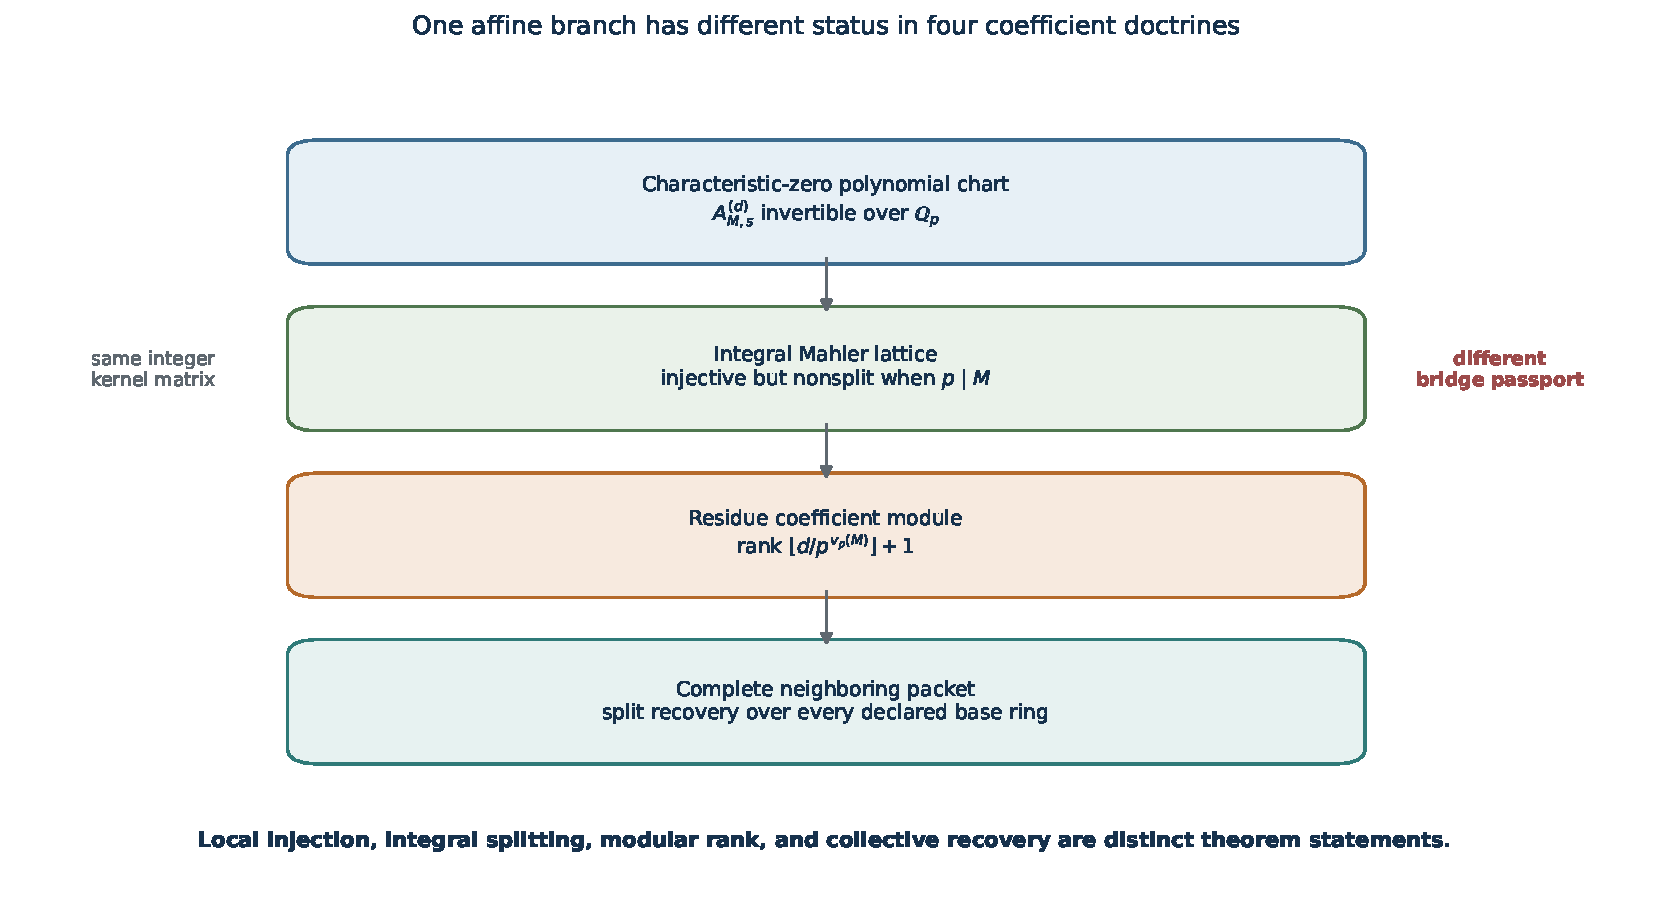
\includegraphics[width=.93\textwidth]{local_channel_ladder.pdf}
\caption{The same affine Mahler kernel has four distinct bridge passports.  Characteristic-zero invertibility, integral injection, modular rank, and complete-packet splitting must not be conflated.}
\label{fig:block08-channel-ladder}
\end{figure}

\begin{figure}[htbp]
\centering
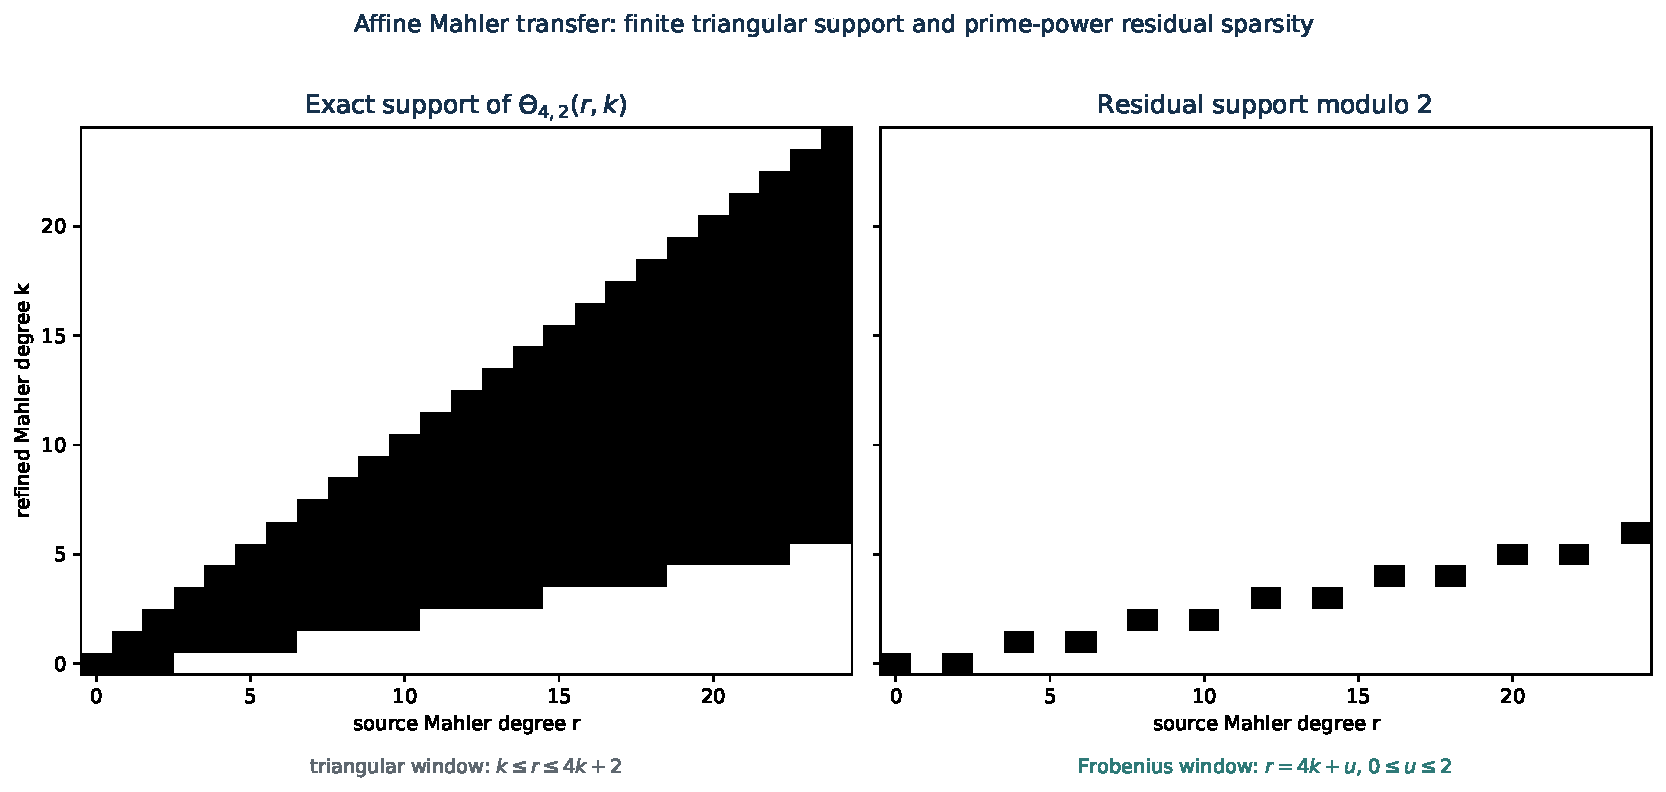
\includegraphics[width=.94\textwidth]{polyphase_kernel_sparsity.pdf}
\caption{The finite triangular support of the affine kernel and its Frobenius-sparse residue pattern at a prime-power radix.}
\label{fig:block08-kernel-sparsity}
\end{figure}

\subsection{Valuation ledgers and Frobenius sparsity}
\label{subsec:block08-valuations}

The coefficient transform carries a precise lower-bound calculus.

\begin{theorem}[Exact branchwise valuation ledger]
\label{thm:block08-valuation-ledger}
For every refined coefficient,
\[
 \boxed{
 v_p(d_{s,k})
 \geq
 \min_{k\leq r\leq Mk+s}
 \left(v_p(c_r)+v_p(\Theta_{M,s}(r,k))\right).}
\]
If \(v_p(c_r)\geq w(r)\) for a nondecreasing weight \(w\), then
\[
 \boxed{v_p(d_{s,k})\geq w(k).}
\]
Thus every declared monotone Mahler precision ladder survives affine polyphase refinement.
\end{theorem}

\begin{proof}
The transfer sum is finite.  Apply the non-Archimedean triangle inequality.  Since \(r\geq k\), monotonicity gives \(w(r)\geq w(k)\), and every kernel entry is integral.
\end{proof}

Define the min-plus certificate transform
\[
 \boxed{
 (\mathfrak W_{M,s}w)(k)
 =
 \min_{k\leq r\leq Mk+s}
 \left(w(r)+v_p(\Theta_{M,s}(r,k))\right).}
\]
This transform is a certified lower bound.  It need not be the exact output valuation, because cancellation can increase the valuation beyond the termwise minimum.

\begin{theorem}[Prime-power Frobenius sparsification]
\label{thm:block08-frobenius-sparsity}
For \(M=p^a\),
\[
 \boxed{
 \Theta_{p^a,s}(r,k)
 \equiv
 \binom{s}{r-p^ak}
 \pmod p,}
\]
where the binomial coefficient is zero outside \(0\leq r-p^ak\leq s\).  Therefore
\[
 \boxed{
 d_{s,k}
 \equiv
 \sum_{u=0}^{s}\binom su c_{p^ak+u}
 \pmod p.}
\]
In particular,
\[
 \boxed{d_{0,k}\equiv c_{p^ak}\pmod p.}
\]
\end{theorem}

\begin{proof}
In characteristic \(p\),
\[
 (1+z)^{p^a}-1\equiv z^{p^a}.
\]
Substitute this into the generating definition of \(\Theta_{p^a,s}\) and compare coefficients.
\end{proof}

\subsection{Carmichael--Mahler state constructors and precision amplification}
\label{subsec:block08-carmichael}

Finite modular state dynamics provide a directional constructor into the local Mahler chart.  Let
\[
 v_{n+1}=Cv_n,
 \qquad
 a_n=w^{\mathsf T}C^nv_0,
\]
with \(C\in M_d(\mathbb Z_p)\) invertible modulo \(p\).

\begin{theorem}[Matrix Carmichael--Mahler constructor]
\label{thm:block08-matrix-carmichael}
Assume
\[
 C^H=I+p^LB,
 \qquad L\geq1.
\]
For every address \(j\),
\[
 \boxed{
 a_{Hx+j}
 =
 \sum_{r\geq0}
 p^{Lr}\binom xr
 w^{\mathsf T}C^jB^rv_0,}
\]
where the series converges for \(x\in\mathbb Z_p\).  Its Mahler coefficients satisfy
\[
 \boxed{v_p(c_{j,r})\geq Lr,}
\]
and
\[
 \boxed{\Delta_H^r a_n\equiv0\pmod{p^{Lr}}.}
\]
\end{theorem}

\begin{proof}
Use
\[
 C^{Hx+j}=C^j(I+p^LB)^x
\]
and expand the principal-unit matrix power by the convergent binomial series.  One forward difference in \(x\) contributes the factor \(p^LB\).
\end{proof}

\begin{theorem}[Principal-unit precision amplification]
\label{thm:block08-precision-amplification}
If \(X=I+p^LB\), then for every \(a\geq0\) there exists \(B_a\in M_d(\mathbb Z_p)\) such that
\[
 \boxed{X^{p^a}=I+p^{L+a}B_a.}
\]
Consequently, for \(H_a=Hp^a\), every branch \(x\mapsto a_{H_ax+j}\) has Mahler coefficients satisfying
\[
 \boxed{v_p(c_{a,j,r})\geq(L+a)r.}
\]
Each additional \(p\)-power refinement contributes at least one further digit of precision per Mahler depth.
\end{theorem}

\begin{proof}
Induct on \(a\).  If \(X_a=I+p^{L+a}B_a\), the binomial expansion of \(X_a^p\) has linear term divisible by \(p^{L+a+1}\), and every higher term has at least the same valuation.  Apply \cref{thm:block08-matrix-carmichael} at the refined jump.
\end{proof}

\begin{example}[Refined dyadic Fibonacci packets]
For the Fibonacci companion matrix
\[
 C=\begin{pmatrix}1&1\\1&0\end{pmatrix},
\]
one has
\[
 C^{12}
 =I+8\begin{pmatrix}29&18\\18&11\end{pmatrix}.
\]
Hence
\[
 \boxed{
 \Delta_{12\cdot2^a}^{\,r}F_n
 \equiv0\pmod{2^{(a+3)r}}.}
\]
\end{example}

\begin{figure}[htbp]
\centering
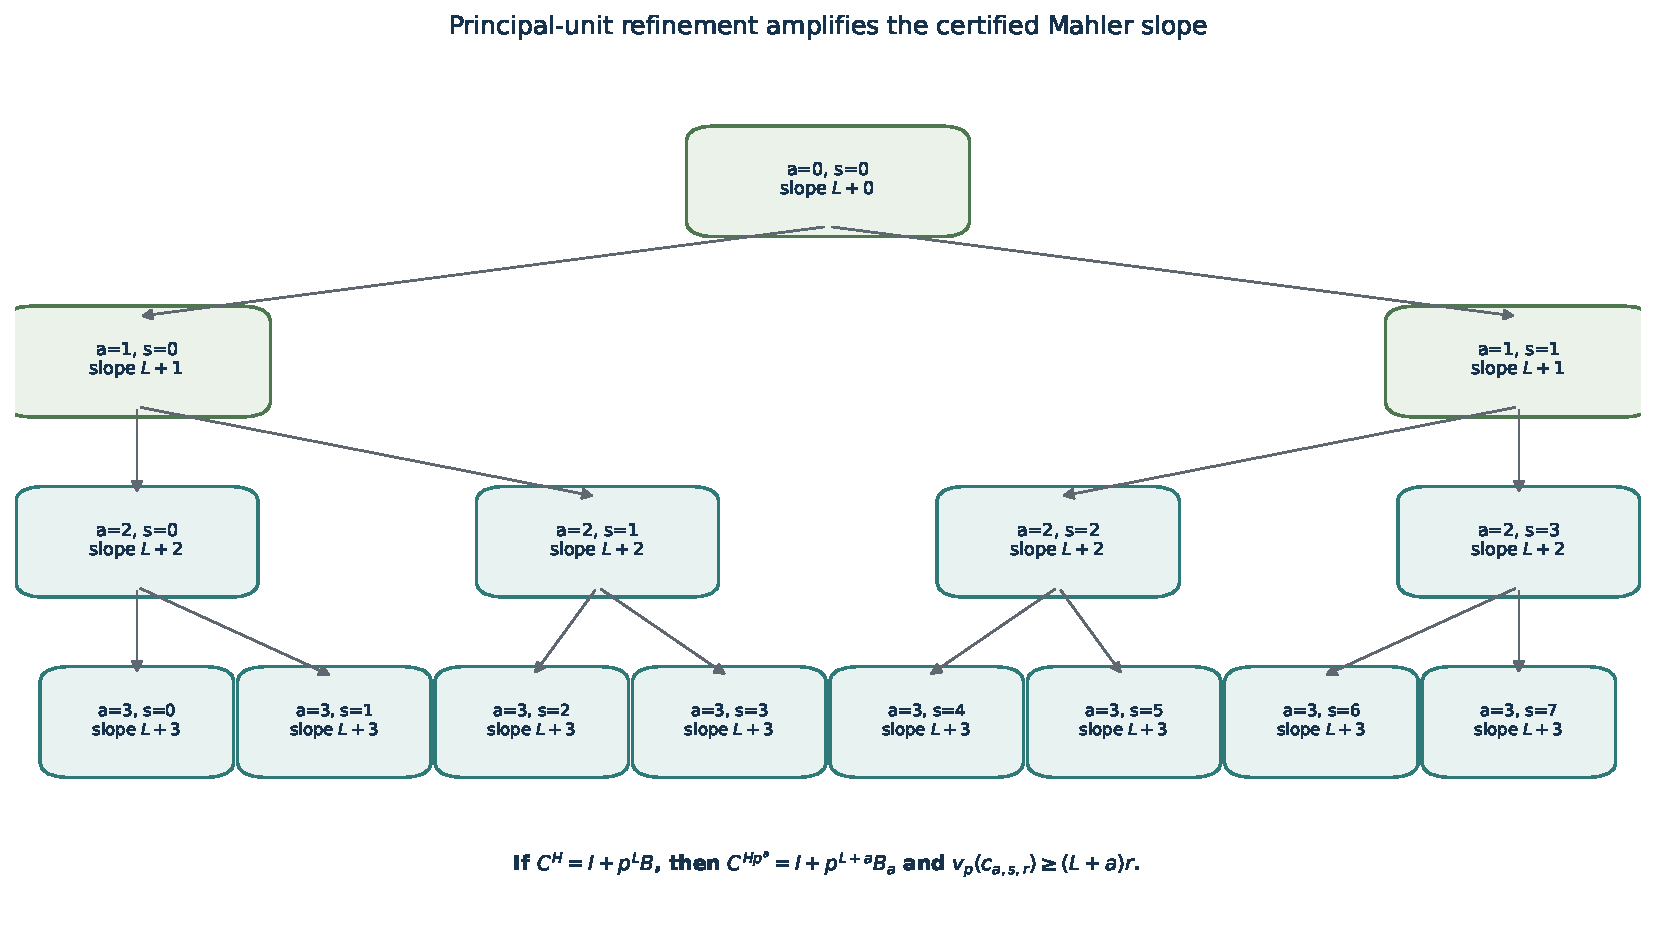
\includegraphics[width=.96\textwidth]{local_precision_tree.pdf}
\caption{A principal-unit state packet acquires one additional guaranteed \(p\)-adic digit per Mahler depth at each \(p\)-power refinement.}
\label{fig:block08-precision-tree}
\end{figure}

The state-to-local construction is directional.  A local branch can forget unreachable state directions, nonminimal coordinates, or modes annihilated by the output functional.  Recovering a state presentation requires a separate recognition or minimality theorem and is not part of the Carmichael--Mahler constructor itself.

\subsection{The exact boundary with functional-Mahler masks}
\label{subsec:block08-functional-boundary}

\begin{proposition}[No canonical unrestricted bridge between the two Mahler channels]
\label{prop:block08-no-unrestricted-mahler-bridge}
Functional-Mahler mask data over \(\mathbb F_p\) does not determine a unique Newton--Mahler chart over \(\mathbb Z_p\), and a continuous Newton--Mahler function does not in general determine a rational functional-Mahler mask.
\end{proposition}

\begin{proof}
A residue sequence \((\bar a_n)\) admits many integral lifts.  If \((a_n)\) is one lift, then \((a_n+pn)\) is another with the same reduction modulo \(p\).  Their Newton--Mahler coefficients differ by the nonzero coefficient sequence of \(pn\).  Thus the residue-series or functional-mask presentation cannot select one local interpolation without a declared lifting rule.

Conversely, a continuous function \(f:\mathbb Z_p\to\mathbb Z_p\) canonically determines its Newton--Mahler coefficients, but rationality of an ordinary generating series or of the mask \(F(z)/F(z^p)\) is an additional property of a separate coefficient-series presentation.  Continuity alone does not supply it.
\end{proof}

\begin{figure}[htbp]
\centering
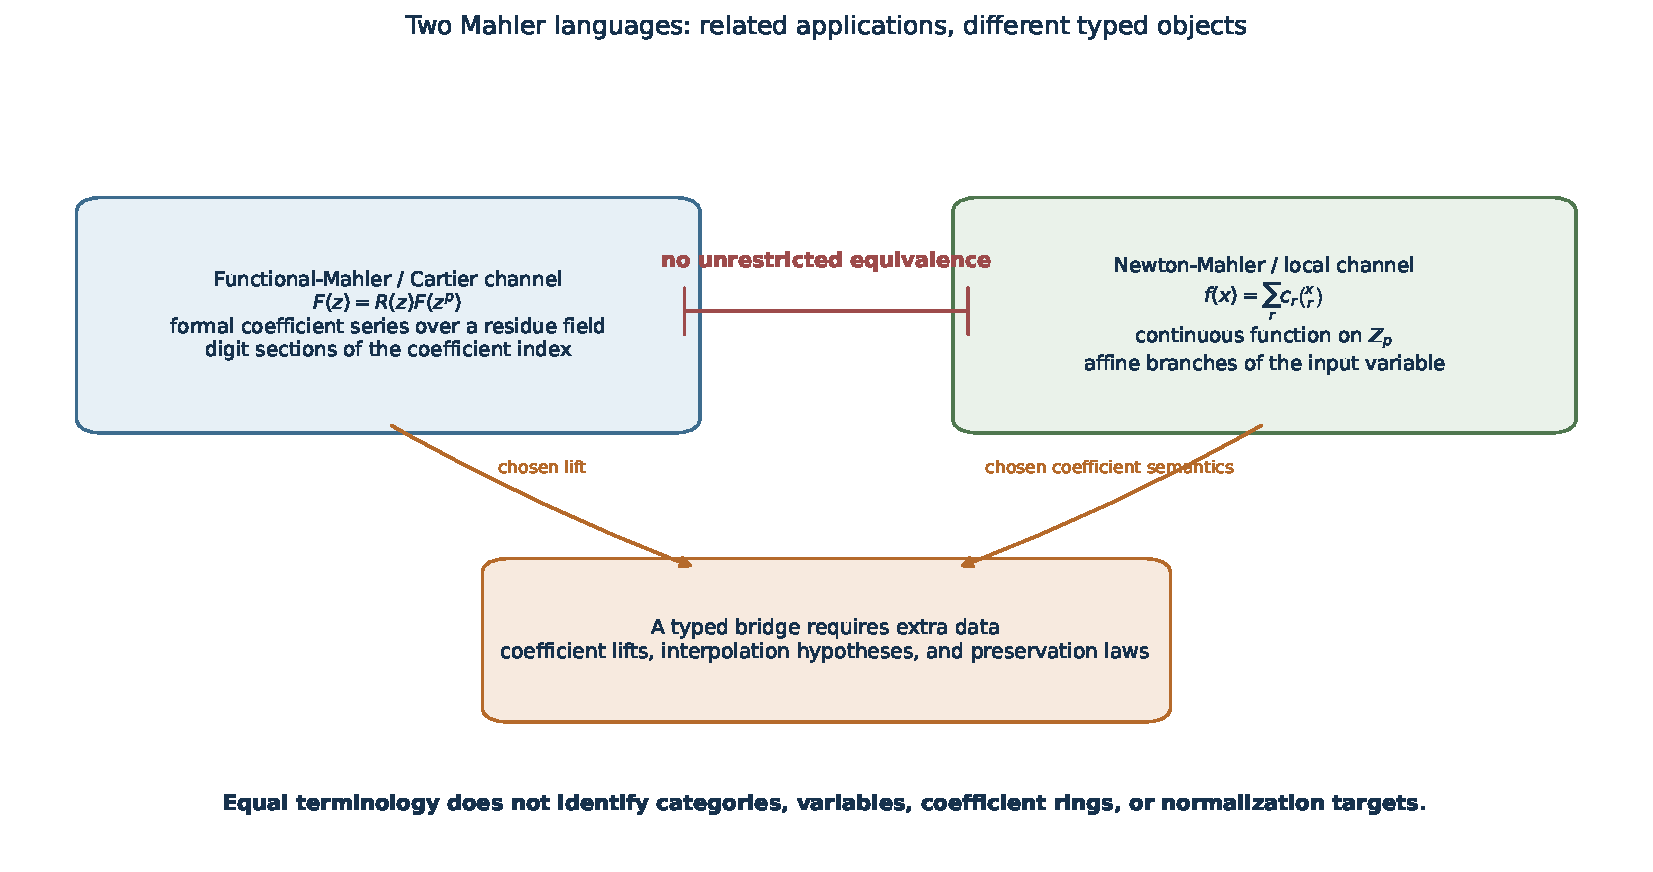
\includegraphics[width=.95\textwidth]{two_mahler_languages.pdf}
\caption{Functional-Mahler and Newton--Mahler constructions require different variables, coefficient doctrines, and normalization data.  A bridge exists only after those extra choices are declared.}
\label{fig:block08-two-mahler-languages}
\end{figure}

\begin{boundarybox}
\textbf{Exact local boundary.}
Local Mahler-polyphase atlas proves a complete normalized atlas for continuous \(\mathbb Z_p\)-valued functions and their complete \(p^a\)-branch packets.  It proves exact affine coefficient transport, mixed-radix coherence, finite-degree characteristic-zero invertibility, integral split recovery, modular rank loss, valuation preservation, and principal-unit precision amplification under the printed hypotheses.  It does not identify every continuous function as locally analytic, compute exact higher valuations of every \(\Theta_{p^a,s}(r,k)\), choose an optimal mixed-radix refinement tree, or construct the combined spectral--local invariant requested by the broader program.
\end{boundarybox}

\subsection{Exact examples and finite verification}
\label{subsec:block08-verification}

For \(f(x)=x^2\), the source Mahler vector is
\[
 (c_0,c_1,c_2)=(0,1,2).
\]
The two dyadic branches are
\[
 f(2q)=4\binom q1+8\binom q2,
\]
and
\[
 f(2q+1)=1+8\binom q1+8\binom q2.
\]
This example exhibits exact finite-window coefficient transport.

For a principal unit \(u=1+p\),
\[
 u^x=\sum_{r\geq0}p^r\binom xr.
\]
The branch \(x=pq\) has coefficients
\[
 \bigl(u^p-1\bigr)^k,
\]
whose valuation is at least \(2k\).  The branch therefore improves the original slope-one certificate.

At \(p=2\), \(M=2\), and \(d=3\), each single reduced channel has rank two, while the two-channel packet has rank four.  This is the smallest visible instance of collective recovery.

\begin{table}[htbp]
\centering
\caption{Exact local Mahler and polyphase examples used in Local Mahler-polyphase atlas.}
\label{tab:block08-examples}
\small
\begin{tabularx}{\textwidth}{@{}L{0.31\textwidth}L{0.29\textwidth}Y@{}}
\toprule
Example & Source Mahler data & Refined data or rank\\
\midrule
\(x^2\), branch 2q+0 & \( (0, 1, 2) \) & \( (0, 4, 8) \)\\
\(x^2\), branch 2q+1 & \( (0, 1, 2) \) & \( (1, 8, 8) \)\\
\((1+2)^x\), branch 2q & \(c_r=2^r,\ 0\leq r\leq4\) & \(d_k=8^k,\ 0\leq k\leq4\)\\
\((1+3)^x\), branch 3q & \(c_r=3^r,\ 0\leq r\leq4\) & \(d_k=63^k,\ 0\leq k\leq4\)\\
\((1+5)^x\), branch 5q & \(c_r=5^r,\ 0\leq r\leq4\) & \(d_k=7775^k,\ 0\leq k\leq4\)\\
mod-2 rank distribution, M=2,d=3 & \( (2, 2) \) & \( (4, 4) \)\\
\bottomrule
\end{tabularx}
\end{table}

\begin{table}[htbp]
\centering
\caption{Local Mahler-polyphase atlas exact verification summary.}
\label{tab:block08-validation}
\small
\begin{tabularx}{\textwidth}{@{}L{0.38\textwidth}Y@{}}
\toprule
Validation class & Recorded result\\
\midrule
Affine-kernel rows & 312 exact row cases\\
Finite coefficient transports & 936 source/chart cases\\
Mixed-radix compositions and CRT diamonds & 2,102 exact diagrams\\
Prime-power rank and sparsity cases & 95 degree/radix cases\\
Integral decoder and composite-minimum cases & 156 cases\\
Valuation-ledger cases & 5,100 coefficient ladders\\
Scalar and matrix precision cases & 923 cases\\
\textbf{Total exact checks} & \textbf{229,743}\\
Failures & 0\\
\bottomrule
\end{tabularx}
\end{table}


The verifier checks the affine generating identity, finite polynomial transport, triangular determinants, mixed-radix composition, Chinese-remainder diamonds, nested branch addresses, prime-power Frobenius sparsity, exact local ranks, packet minimality, integer decoders, composite primary minima, valuation ledgers, scalar principal-unit amplification, and the refined Fibonacci matrix congruences.  It also includes a negative control showing that equal residue data can have distinct Newton--Mahler lifts.

\begin{resultbox}
\textbf{Local Mahler--polyphase result.}
The local continuous, Newton--Mahler coefficient, complete clopen branch, and branch-coefficient presentations form an effective normalized atlas.  Affine polyphase kernels compose strictly and transport declared valuation ladders.  The finite-degree restriction exposes a four-level bridge ladder: reversible characteristic-zero charts, nonsplit integral channels, rank-deficient residue channels, and split neighboring packets.  Carmichael--Mahler transfer embeds finite principal-unit state dynamics into the local atlas with a certified precision slope that improves under \(p\)-power refinement.  Functional-Mahler masks remain a distinct typed channel unless coefficient lifts and interpolation data are supplied.
\end{resultbox}


\section{Holonomic Ore charts, multisection modules, and a Fuchsian packet theorem}
\label{sec:block09-holonomic}

Holonomic atlas develops the next native stratum in the declared work program.  The general holonomic problem has two logically separate parts.  First, a D-finite series and its P-recursive coefficient sequence require normalized operator charts that remember the finite initial data lost by tail recurrences.  Second, arithmetic multisection preserves holonomicity but can change minimal order through root-orbit aliasing, resonance, and address-dependent cancellation.  The first part is closed here on the ordinary-point locus.  The second is organized in general and solved exactly for a nontrivial regular-singular family.

Throughout this section, $K$ is a characteristic-zero field.  When local monodromy is discussed, $K$ is embedded in $\mathbb C$ and all local exponents are taken over an algebraic closure.

\subsection{Ore annihilators and normalized holonomic charts}
\label{subsec:block09-ore}

Let
\[
 \mathcal D_K=K(z)\langle D\rangle,
 \qquad
 Dq=qD+q',
\]
be the differential Ore algebra, and let
\[
 \mathcal S_K=K(n)\langle S\rangle,
 \qquad
 Sq(n)=q(n+1)S,
\]
be the forward-shift Ore algebra.  Both are Euclidean skew-polynomial rings in their operator variable, so their nonzero left ideals have unique monic generators \cite{Ore1933}.

\begin{definition}[Minimal differential annihilator]
For a nonzero D-finite series $F\in K[[z]]$, define
\[
 \operatorname{Ann}_{\mathcal D}(F)
 =
 \{L\in\mathcal D_K:LF=0\}.
\]
Its unique monic generator is denoted
\[
 \boxed{L_F.}
\]
The differential order
\[
 r_D(F)=\operatorname{ord}_D L_F
\]
is the minimal scalar differential order of $F$ over $K(z)$.
\end{definition}

\begin{definition}[Minimal tail recurrence]
For a sequence $a=(a_n)_{n\geq0}$, define its tail annihilator by
\[
 \operatorname{Ann}_{\rm tail}(a)
 =
 \{R\in\mathcal S_K:(Ra)_n=0\text{ for all sufficiently large }n\}.
\]
For a non-eventually-zero P-recursive sequence, its unique monic generator is denoted
\[
 \boxed{R_a.}
\]
If the sequence is eventually zero, the tail generator is $1$ and has order zero.
\end{definition}

Write
\[
 R_a
 =
 S^s+\sum_{j=0}^{s-1}r_j(n)S^j.
\]
Let $\nu_a$ be the least index from which $R_a$ annihilates the sequence, and define $N_a$ to be the least integer $N\geq\nu_a$ larger than every nonnegative pole of the rational functions $r_j(n)$.  Then
\[
 \mathfrak R(a)
 =
 \bigl(R_a,N_a,a_0,\ldots,a_{N_a+s-1}\bigr)
\]
is a canonical complete recurrence chart.  The operator controls the tail, while the finite prefix crosses every singular index and fixes the exact sequence rather than only its eventual equivalence class.

\begin{proposition}[Derivative-module rank]
\label{prop:block09-derivative-rank}
For a nonzero D-finite series $F$,
\[
 \boxed{
 r_D(F)
 =
 \dim_{K(z)}\operatorname{span}_{K(z)}
 \{F,DF,D^2F,\ldots\}.}
\]
\end{proposition}

\begin{proof}
A differential operator of order $r$ gives a linear dependence among $F,DF,\ldots,D^rF$.  Minimality of $L_F$ says that no dependence exists among the first $r$ derivative vectors.  Therefore they form a basis of the derivative span.
\end{proof}

\subsection{The exact coefficient bridge}
\label{subsec:block09-coefficient-bridge}

The classical equivalence between P-recursive sequences and D-finite ordinary generating functions is effective in both directions \cite{Stanley1980}.  The following formulas make the finite residual explicit.

Let
\[
 F(z)=\sum_{n\geq0}a_nz^n
\]
and
\[
 L
 =
 \sum_{j=0}^{r}q_j(z)D^j,
 \qquad
 q_j(z)=\sum_{m=0}^{d_j}q_{j,m}z^m.
\]

\begin{theorem}[Differential-to-recurrence coefficient formula]
\label{thm:block09-diff-to-rec}
For every $n\geq0$,
\[
 \boxed{
 [z^n]LF
 =
 \sum_{j=0}^{r}
 \sum_{m=0}^{\min(d_j,n)}
 q_{j,m}
 (n-m+j)^{\underline{j}}
 a_{n-m+j},}
\]
where
\[
 x^{\underline j}=x(x-1)\cdots(x-j+1).
\]
Consequently, every polynomial-coefficient differential equation yields an explicit polynomial recurrence after a finite reindexing.
\end{theorem}

\begin{proof}
The coefficient of $z^{n-m}$ in $D^jF$ is
\[
 (n-m+j)^{\underline j}a_{n-m+j}.
\]
Multiplication by $q_{j,m}z^m$ shifts that contribution to degree $n$.  Summing over $j$ and $m$ gives the formula.
\end{proof}

Conversely, suppose
\[
 \sum_{s=0}^{q}p_s(n)a_{n+s}=0
 \qquad(n\geq N),
\]
where $p_s\in K[n]$, and put
\[
 \theta=zD.
\]

\begin{theorem}[Recurrence residual as an Euler-operator polynomial]
\label{thm:block09-rec-to-diff}
Define
\[
 \boxed{
 Q
 =
 \sum_{s=0}^{q}
 z^{q-s}p_s(\theta-s).}
\]
Then
\[
 \boxed{
 [z^{n+q}]QF
 =
 \sum_{s=0}^{q}p_s(n)a_{n+s}.}
\]
Hence $QF$ is a polynomial of degree less than $N+q$, and
\[
 \boxed{D^{N+q}QF=0.}
\]
\end{theorem}

\begin{proof}
The operator $p_s(\theta-s)$ multiplies the coefficient of $z^k$ by $p_s(k-s)$.  After multiplication by $z^{q-s}$, the coefficient at $z^{n+q}$ is $p_s(n)a_{n+s}$.  The recurrence kills every coefficient from degree $N+q$ onward.  Differentiating more times than the residual degree gives a homogeneous annihilator.
\end{proof}

The polynomial residual is not noise.  It is the exact finite-prefix certificate that distinguishes a recurrence valid only in the tail from an identity in the full formal-series chart.

\subsection{The ordinary-point holonomic atlas}
\label{subsec:block09-ordinary-atlas}

\begin{definition}[Ordinary-point locus]
A nonzero D-finite series $F\in K[[z]]$ belongs to
\[
 \mathbf{Hol}^{\rm ord}_K
\]
when its monic minimal operator can be written
\[
 L_F
 =
 D^r+\sum_{j=0}^{r-1}\ell_j(z)D^j
\]
with every $\ell_j$ regular at $z=0$.
\end{definition}

The normalized jet is
\[
 J_0(F)
 =
 \bigl(F(0),F'(0),\ldots,F^{(r-1)}(0)\bigr).
\]

\begin{theorem}[Ordinary-point reconstruction]
\label{thm:block09-ordinary-reconstruction}
Let
\[
 L=D^r+\sum_{j=0}^{r-1}\ell_j(z)D^j
\]
with all $\ell_j$ regular at zero.  For every jet
\[
 (y_0,\ldots,y_{r-1})\in K^r
\]
there is a unique formal series $F\in K[[z]]$ satisfying
\[
 LF=0,
 \qquad
 F^{(j)}(0)=y_j.
\]
\end{theorem}

\begin{proof}
Write $F(z)=\sum c_nz^n$.  At coefficient degree $n$, the monic term $D^rF$ contributes
\[
 \frac{(n+r)!}{n!}c_{n+r},
\]
while every lower derivative involves only $c_0,\ldots,c_{n+r-1}$.  Characteristic zero makes the displayed coefficient invertible.  The equation therefore determines $c_{n+r}$ recursively from the jet.
\end{proof}

\begin{theorem}[Normalized ordinary holonomic atlas]
\label{thm:block09-ordinary-atlas}
On the ordinary-point locus, the following normalized presentations determine one another exactly:
\[
 \boxed{
 \begin{aligned}
 &F\in K[[z]],\\
 &(L_F,J_0(F)),\\
 &\operatorname{span}_{K(z)}\{D^jF:j\geq0\}
   \text{ with cyclic vector }F,\\
 &(R_a,N_a,a_0,\ldots,a_{N_a+s-1}),
 \qquad a_n=[z^n]F.
 \end{aligned}}
\]
With equality morphisms, these charts form equivalent normalized groupoids, and every fiber over a fixed semantic series is contractible.
\end{theorem}

\begin{proof}
The series gives its unique minimal Ore operators and finite data.  The derivative module recovers $L_F$ as the first monic dependence among consecutive derivatives.  The operator and jet recover $F$ by \cref{thm:block09-ordinary-reconstruction}.  The recurrence chart reconstructs every coefficient after its singular prefix.  The two explicit coefficient formulas transport between the differential and recurrence channels.  Minimal monic normalization removes coordinate automorphisms, so each normalized fiber has only the identity.
\end{proof}

\begin{figure}[htbp]
\centering
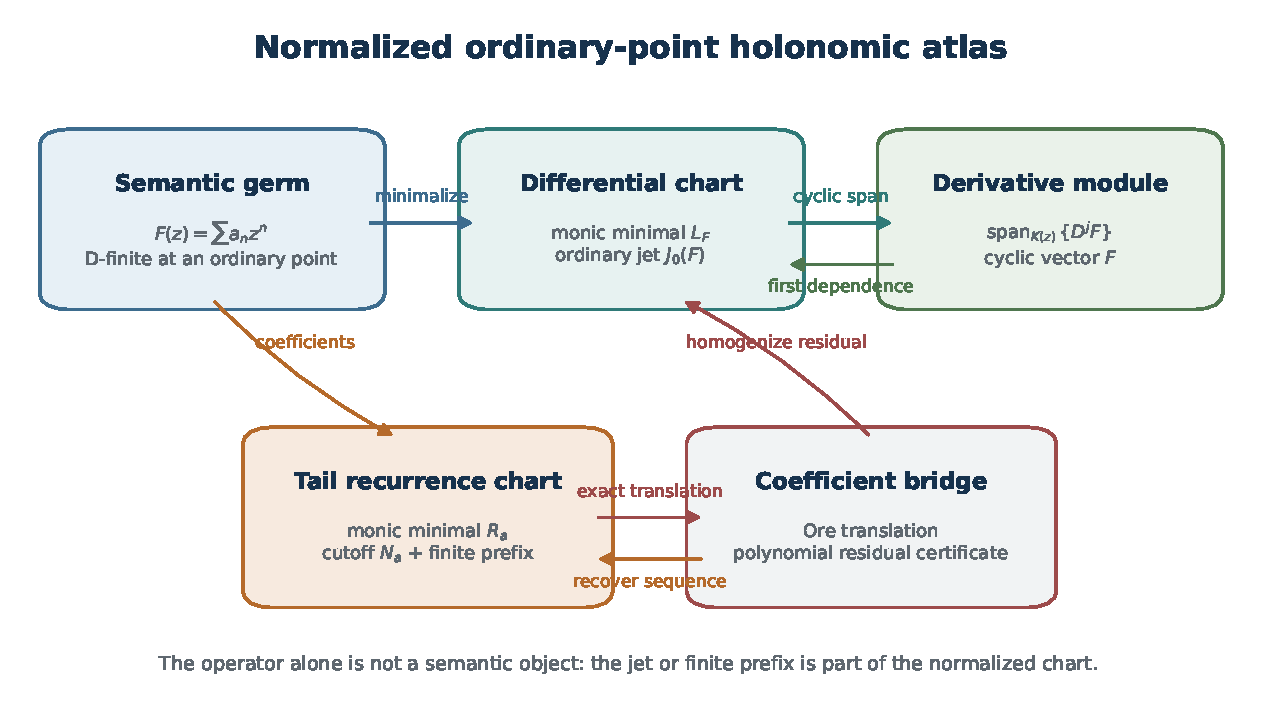
\includegraphics[width=.97\textwidth]{holonomic_ore_atlas.pdf}
\caption{The ordinary holonomic atlas keeps the semantic series, minimal differential operator and jet, cyclic derivative module, and minimal tail recurrence with singular prefix as separate normalized charts.}
\label{fig:block09-ore-atlas}
\end{figure}

\subsection{General arithmetic multisection}
\label{subsec:block09-general-multisection}

For $N\geq1$ and $0\leq j<N$, define
\[
 \mathfrak M_{N,j}F(x)
 =
 \sum_{m\geq0}a_{Nm+j}x^m.
\]
If $\omega_N$ is a primitive $N$th root of unity and $x=t^N$, then
\[
 \boxed{
 t^j\mathfrak M_{N,j}F(t^N)
 =
 \frac1N
 \sum_{q=0}^{N-1}
 \omega_N^{-jq}F(\omega_N^qt).}
\]
This is the character projector for the cyclic rotation action.

\begin{theorem}[Holonomic multisection closure]
\label{thm:block09-multisection-closure}
If $F$ is D-finite, then every $\mathfrak M_{N,j}F$ is D-finite.  Equivalently, arithmetic sections of P-recursive sequences are P-recursive.
\end{theorem}

\begin{proof}
The root-filter formula uses finitely many algebraic substitutions and a finite linear combination.  D-finite series are closed under those operations.  The resulting section has coefficients in the original base field, so the operator descends.
\end{proof}

Closure does not determine the smallest operator.  A separate exact state construction gives a useful bound.

\begin{theorem}[Nonautonomous state jump]
\label{thm:block09-state-jump}
Suppose a P-recursive sequence is represented, beyond its singular prefix, by
\[
 v_{n+1}=C(n)v_n,
 \qquad
 a_n=\lambda(n)v_n,
\]
where $v_n\in K^s$ and $C(n)$ is rational.  Then the $j$th $N$-section has the jump system
\[
 \boxed{
 w_{m+1}=J_{N,j}(m)w_m,}
\]
where
\[
 \boxed{
 J_{N,j}(m)
 =
 C(Nm+j+N-1)\cdots C(Nm+j).}
\]
After denominator clearing, every scalar output has a polynomial recurrence of order at most $s$.
\end{theorem}

\begin{proof}
Compose the $N$ consecutive one-step transfers.  The $s+1$ consecutive scalar output rows are linearly dependent over $K(m)$, producing a recurrence of order at most $s$.
\end{proof}

The root filter also gives a construction-independent order ledger before the algebraic descent from $t$ to $x=t^N$.  Work over a finite extension $E/K$ containing $\omega_N$.  Put
\[
 F_q(t)=F(\omega_N^qt),
 \qquad
 G_{N,j}(t)=\frac1N\sum_{q=0}^{N-1}\omega_N^{-jq}F_q(t).
\]
Let $L_q\in E(t)\langle D_t\rangle$ be the monic minimal annihilator of $F_q$.  Rotation is an Ore-algebra automorphism, so every $L_q$ has order $r=\operatorname{ord}L_F$.  Let
\[
 L_N^{\rm orb}=\operatorname{LCLM}(L_0,\ldots,L_{N-1}),
 \qquad
 r_N^{\rm orb}=\operatorname{ord}L_N^{\rm orb},
\]
and, when $G_{N,j}\neq0$, let $L_{N,j}^{\rm char}$ be its monic minimal annihilator with order $r_{N,j}^{\rm char}$.  For a zero character packet put $r_{N,j}^{\rm char}=0$.

\begin{definition}[Root-filter alias and address-cancellation defects]
\label{def:block09-general-defects}
Define
\[
 \mathfrak a_N(F)=Nr-r_N^{\rm orb},
 \qquad
 \mathfrak c_{N,j}(F)=r_N^{\rm orb}-r_{N,j}^{\rm char}.
\]
The first quantity measures dependence already present among the rotated holonomic modules.  The second measures the additional loss caused by the $j$th character projector after the rotated orbit has been assembled.
\end{definition}

\begin{theorem}[Exact two-stage root-filter defect identity]
\label{thm:block09-general-defect-identity}
The defects in \cref{def:block09-general-defects} are nonnegative and satisfy
\[
 \boxed{
 Nr-r_{N,j}^{\rm char}
 =
 \mathfrak a_N(F)+\mathfrak c_{N,j}(F).}
\]
Thus orbit aliasing occurs before address selection, while address cancellation occurs after the Fourier character has been applied.
\end{theorem}

\begin{proof}
The least common left multiple has order at most the sum of the orders of its inputs, hence $r_N^{\rm orb}\leq Nr$.  It annihilates every rotated series and therefore annihilates their character sum $G_{N,j}$.  By minimality, $L_N^{\rm orb}$ belongs to the principal left annihilator ideal generated by $L_{N,j}^{\rm char}$ whenever the character sum is nonzero, so $r_{N,j}^{\rm char}\leq r_N^{\rm orb}$.  The zero case is immediate.  The displayed identity is the telescoping decomposition
\[
 Nr-r_{N,j}^{\rm char}
 =
 (Nr-r_N^{\rm orb})+(r_N^{\rm orb}-r_{N,j}^{\rm char}).
\]
\end{proof}

\begin{boundarybox}
\textbf{Root-filter order versus packet order.}
The preceding theorem is exact in the rotated $t$-coordinate over $E(t)$.  The arithmetic packet is the series $\mathfrak M_{N,j}F(x)$ over the base field, related by
\[
 G_{N,j}(t)=t^j\mathfrak M_{N,j}F(t^N).
\]
Algebraic pullback, base extension, gauge multiplication, and descent may change the minimal scalar operator visible in the $x$-chart.  That comparison is a separately typed descent problem.  The exact binomial--Fuchsian family below computes both sides and therefore resolves this additional step in a nontrivial model case.
\end{boundarybox}

Let $Q^{\rm cl}_{N,j}$ be an annihilator produced by a declared closure or elimination pipeline, and let $L_{N,j}$ be the monic minimal operator of the section.  Since every annihilator belongs to the principal left ideal generated by $L_{N,j}$,
\[
 Q^{\rm cl}_{N,j}=A_{N,j}L_{N,j}
\]
for some Ore operator $A_{N,j}$.  The nonnegative quantity
\[
 \delta^{\rm cl}_{N,j}
 =
 \operatorname{ord}Q^{\rm cl}_{N,j}
 -
 \operatorname{ord}L_{N,j}
\]
measures cancellation relative to that construction.  It is not intrinsic until the construction has been fixed.

\subsection{Operator singularities and local exponent packets}
\label{subsec:block09-local-exponents}

Multiply $L_F$ by a common denominator, divide the polynomial coefficients by their greatest common divisor, and normalize the leading coefficient to be monic.  This gives a unique primitive polynomial representative
\[
 \widetilde L_F
 =
 \sum_{j=0}^{r}q_j(z)D^j.
\]
Its operator singular support is
\[
 \Sigma_{\rm op}(F)
 =
 \{q_r(z)=0\}\cup\{\infty\}.
\]
Apparent singularities remain part of this operator coordinate until an explicit desingularization has been performed.

Let $\alpha$ be a finite point and put
\[
 v_j=v_\alpha(q_j),
 \qquad
 \mu=\min_j(v_j-j).
\]
Write the first nonzero local coefficient of $q_j$ as $q_{j,v_j}$.  The indicial polynomial is
\[
 \boxed{
 I_{\alpha,L}(\rho)
 =
 \sum_{v_j-j=\mu}
 q_{j,v_j}\rho^{\underline j}.}
\]
At a regular singular point, its roots form the local exponent packet.  Over $\mathbb C$, the corresponding local monodromy eigenvalues are
\[
 e^{2\pi i\rho}.
\]
Integer differences between exponents signal resonance.  Exponent eigenvalues alone do not determine logarithmic extension data or the full monodromy conjugacy class.

\begin{proposition}[Singularity orbit under multisection]
\label{prop:block09-singularity-orbit}
Assume $F$ is an analytic germ at zero with analytic continuation away from a finite set $\Sigma$.  Then every finite nonzero analytic singularity of $\mathfrak M_{N,j}F$ lies in
\[
 \boxed{
 \Sigma^{[N]}
 =
 \{\alpha^N:\alpha\in\Sigma\}.}
\]
Distinct singularities in one fiber of $\alpha\mapsto\alpha^N$ are aliased by the multisection map.  A character projection may remove some aliased local contributions.
\end{proposition}

\begin{proof}
Away from $\Sigma^{[N]}$ and zero, choose a local analytic branch $t=x^{1/N}$.  Every rotated argument $\omega_N^qt$ avoids $\Sigma$, so the root-filter expression is analytic.  A singularity can therefore occur only when one rotated preimage meets $\Sigma$.
\end{proof}

At nonzero regular singular points, the map $t\mapsto t^N$ is unramified.  It preserves local exponents before character projection.  At zero and infinity it is ramified, so exponent scaling must be recorded separately.

\subsection{An exact binomial--Fuchsian packet family}
\label{subsec:block09-binomial-family}

The general minimal multisection problem remains open.  The family
\[
 \boxed{
 F_{\lambda,\alpha}(z)
 =
 (1-\alpha z)^{-\lambda}}
\]
provides a nontrivial exact model that contains irreducible Fuchsian packets, rational collapse, finite-support aliasing, and zero-address cancellation in one parameter space.

Its coefficients are
\[
 a_n
 =
 \frac{(\lambda)_n}{n!}\alpha^n.
\]
For $0\leq j<N$, put
\[
 G_{N,j}^{\lambda,\alpha}(x)
 =
 \sum_{m\geq0}
 \frac{(\lambda)_{Nm+j}}{(Nm+j)!}
 \alpha^{Nm+j}x^m.
\]
Define the upper and lower parameter packets
\[
 A_{N,j}(\lambda)
 =
 \left\{
 \frac{\lambda+j+r}{N}:0\leq r<N
 \right\},
\]
\[
 B_{N,j}
 =
 \left\{
 \frac{j+1+r}{N}:0\leq r<N
 \right\}\setminus\{1\}.
\]

\begin{theorem}[Exact hypergeometric packet form]
\label{thm:block09-hypergeom-packet}
If $(\lambda)_j\neq0$, then
\[
 \boxed{
 G_{N,j}^{\lambda,\alpha}(x)
 =
 \frac{(\lambda)_j\alpha^j}{j!}
 {}_NF_{N-1}
 \!\left(
 \begin{matrix}A_{N,j}(\lambda)\\ B_{N,j}\end{matrix}
 ;\alpha^Nx
 \right).}
\]
Its coefficients satisfy the first-order polynomial recurrence
\[
 \boxed{
 \prod_{r=0}^{N-1}(Nm+j+1+r)u_{m+1}
 =
 \alpha^N
 \prod_{r=0}^{N-1}(Nm+j+\lambda+r)u_m.}
\]
The series is annihilated by
\[
 \boxed{
 \mathcal H_{N,j}^{\lambda,\alpha}
 =
 \theta
 \prod_{b\in B_{N,j}}(\theta+b-1)
 -
 \alpha^Nx
 \prod_{a\in A_{N,j}(\lambda)}(\theta+a),}
\]
where $\theta=xD_x$.
\end{theorem}

\begin{proof}
Split the rising factorials and ordinary factorials into their $N$ residue factors.  The multiplication formula gives the displayed hypergeometric coefficients.  Taking the ratio of consecutive packet coefficients gives the recurrence.  Coefficient comparison with the standard ${}_NF_{N-1}$ operator gives the differential equation.
\end{proof}

\begin{theorem}[Minimal differential order phase diagram]
\label{thm:block09-order-phase}
Let
\[
 r_D(N,j;\lambda)
 =
 r_D\bigl(G_{N,j}^{\lambda,\alpha}\bigr),
 \qquad \alpha\neq0.
\]
Then:

\begin{enumerate}
\item If $\lambda\notin\mathbb Z$, then
\[
 \boxed{r_D(N,j;\lambda)=N.}
\]
\item If $\lambda=L\in\mathbb Z_{>0}$, then every packet is a nonzero rational function with exact denominator
\[
 (1-\alpha^Nx)^L,
\]
and
\[
 \boxed{r_D(N,j;L)=1.}
\]
\item If $\lambda=-M\in\mathbb Z_{\leq0}$, then $G_{N,j}^{-M,\alpha}$ is zero when $j>M$.  Otherwise it is a nonzero polynomial of degree
\[
 \left\lfloor\frac{M-j}{N}\right\rfloor
\]
and
\[
 \boxed{
 r_D(N,j;-M)
 =
 \begin{cases}
 1,&j\leq M,\\
 0,&j>M.
 \end{cases}}
\]
\end{enumerate}
\end{theorem}

\begin{proof}
For nonintegral $\lambda$, no difference between an upper parameter and a completed lower parameter is an integer.  The classical irreducibility criterion for generalized hypergeometric operators therefore makes $\mathcal H_{N,j}^{\lambda,\alpha}$ irreducible of order $N$ \cite{BeukersHeckman1989}.  Since the packet is nonzero, its minimal operator has order $N$.

For $L>0$, the coefficient is a polynomial of degree $L-1$ in $m$ times $\alpha^{Nm+j}$.  Its generating function is rational with denominator $(1-\alpha^Nx)^L$, and the leading polynomial term prevents cancellation of the highest denominator power.  Every nonconstant rational function has a first-order logarithmic-derivative annihilator.

For $\lambda=-M$, the source series is the polynomial $(1-\alpha z)^M$.  Selecting one residue class leaves exactly the displayed finite support.  A nonzero polynomial has differential order one, while the zero function has order zero.
\end{proof}

The tail recurrence order and differential order are different invariants.  A nonzero finite-support coefficient sequence has tail recurrence order zero but its polynomial generating function has differential order one.

\subsection{Orbit aliasing and address cancellation}
\label{subsec:block09-alias-cancellation}

Let $\omega_N$ be primitive and consider the rotated orbit
\[
 \mathcal O_N(F_{\lambda,\alpha})
 =
 \left
 \{(1-\alpha\omega_N^rt)^{-\lambda}:0\leq r<N\right\}.
\]
Let $r_{\rm orb}$ be its dimension over the constant field.

\begin{theorem}[Exact orbit rank]
\label{thm:block09-orbit-rank}
For the binomial family,
\[
 \boxed{
 r_{\rm orb}(N;\lambda)
 =
 \begin{cases}
 N,&\lambda\notin\mathbb Z_{\leq0},\\
 \min(N,M+1),&\lambda=-M\in\mathbb Z_{\leq0}.
 \end{cases}}
\]
\end{theorem}

\begin{proof}
If $\lambda$ is nonintegral, each rotated branch has a branch singularity at a different point.  If $\lambda$ is a positive integer, each has a pole at a different point.  A constant linear relation would therefore have zero coefficient at every branch.

If $\lambda=-M$, expand
\[
 (1-\alpha\omega_N^rt)^M
 =
 \sum_{n=0}^{M}
 \binom Mn(-\alpha)^n\omega_N^{rn}t^n.
\]
The rotation matrix is a truncated discrete Fourier matrix.  Its rank is the number of available residue classes, namely $\min(N,M+1)$.
\end{proof}

Define the alias and cancellation deficits by
\[
 \boxed{
 A_N(\lambda)=N-r_{\rm orb}(N;\lambda),}
\]
\[
 \boxed{
 C_{N,j}(\lambda)
 =
 r_{\rm orb}(N;\lambda)
 -r_D(N,j;\lambda).}
\]
Then
\[
 \boxed{
 N-r_D(N,j;\lambda)
 =
 A_N(\lambda)+C_{N,j}(\lambda).}
\]

\begin{corollary}[Exact defect formulas]
\label{cor:block09-defect-formulas}
The three parameter regimes have the following signatures.

\begin{enumerate}
\item If $\lambda\notin\mathbb Z$, then
\[
 A_N(\lambda)=0,
 \qquad
 C_{N,j}(\lambda)=0.
\]
\item If $\lambda=L>0$, then
\[
 A_N(L)=0,
 \qquad
 C_{N,j}(L)=N-1.
\]
\item If $\lambda=-M\leq0$, then
\[
 A_N(-M)=\max(0,N-M-1),
\]
and
\[
 C_{N,j}(-M)
 =
 \begin{cases}
 \min(N,M+1)-1,&j\leq M,\\
 \min(N,M+1),&j>M.
 \end{cases}
\]
\end{enumerate}
\end{corollary}

This separates two mechanisms that are easily conflated.  Orbit aliasing occurs before an address is selected.  Address cancellation occurs after the Fourier projector has been applied.

\begin{figure}[htbp]
\centering
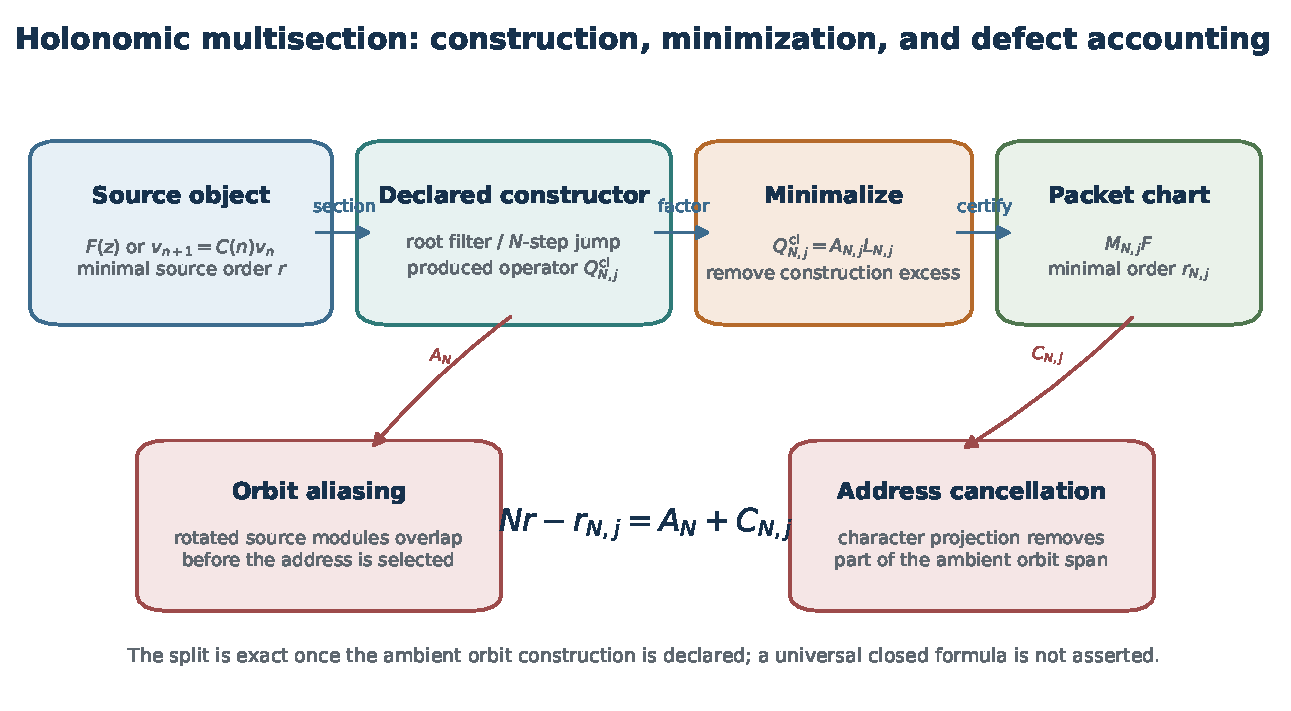
\includegraphics[width=.97\textwidth]{holonomic_multisection_pipeline.pdf}
\caption{The declared holonomic multisection pipeline.  General closure constructs an annihilator but does not prove minimality.  The binomial--Fuchsian family admits an exact orbit-rank and address-cancellation decomposition.}
\label{fig:block09-multisection-pipeline}
\end{figure}

\begin{figure}[htbp]
\centering
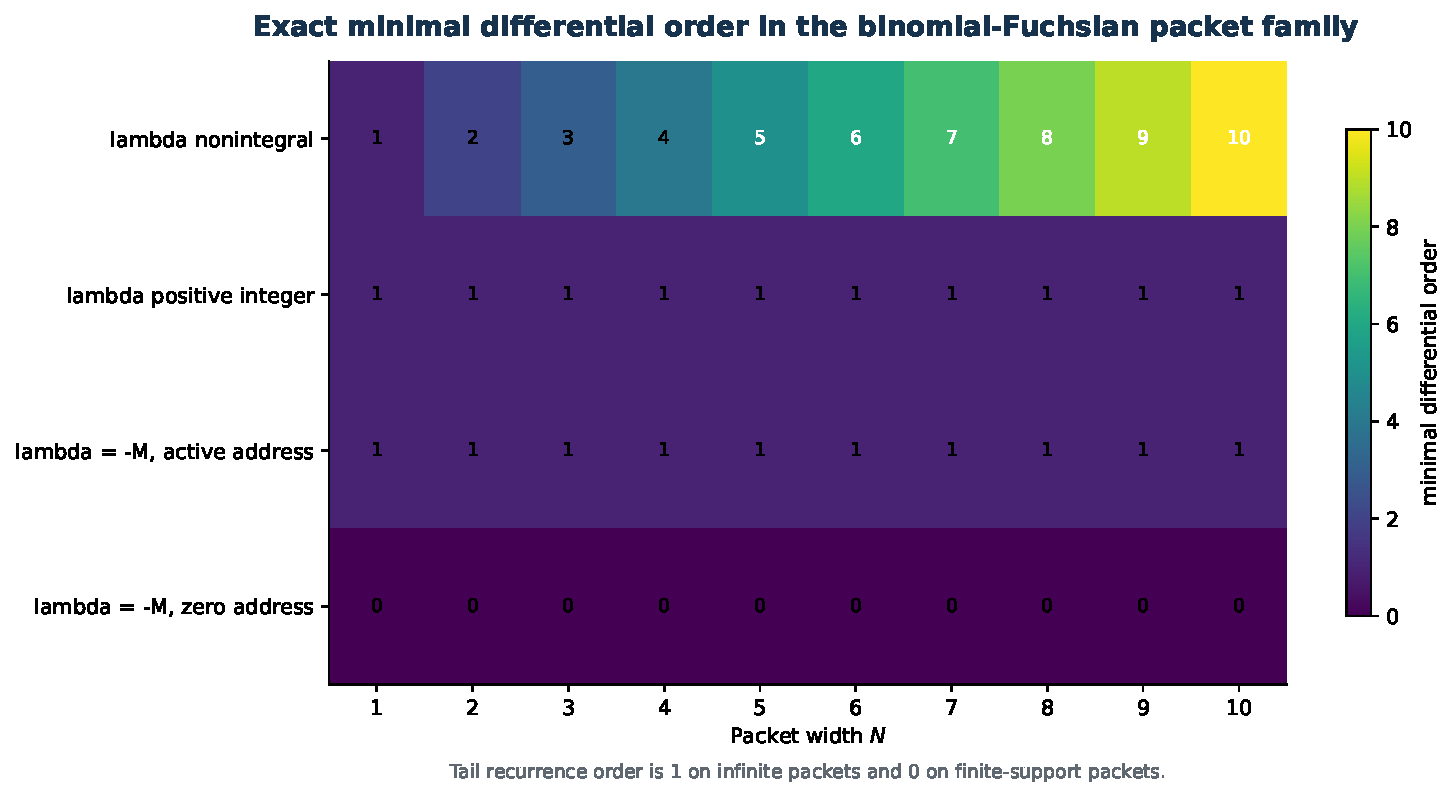
\includegraphics[width=.96\textwidth]{holonomic_order_phase.pdf}
\caption{Minimal differential order in the binomial packet family.  Nonintegral exponents retain order $N$, positive integers collapse to rational order one, and nonpositive integers terminate with explicit aliasing and zero-address packets.}
\label{fig:block09-order-phase}
\end{figure}

\subsection{Local exponent and monodromy packet}
\label{subsec:block09-fuchsian-exponents}

For $\lambda\notin\mathbb Z$, the hypergeometric operator in \cref{thm:block09-hypergeom-packet} is Fuchsian with singularities
\[
 \boxed{
 0,
 \qquad
 \alpha^{-N},
 \qquad
 \infty.}
\]
Its exponent packets are
\[
 \boxed{
 E_0
 =
 \{0\}\cup\{1-b:b\in B_{N,j}\},}
\]
\[
 \boxed{
 E_{\alpha^{-N}}
 =
 \{0,1,\ldots,N-2,-\lambda\},}
\]
and
\[
 \boxed{
 E_\infty
 =
 A_{N,j}(\lambda).}
\]
Modulo integers, $E_0$ is the complete $N$-torsion set
\[
 \left\{0,\frac1N,\ldots,\frac{N-1}{N}\right\},
\]
and the pairwise differences in $E_\infty$ are also $N$-torsion.

\begin{proposition}[Local monodromy ledger]
\label{prop:block09-local-monodromy}
For nonintegral rational $\lambda$:

\begin{enumerate}
\item the monodromy eigenvalues at zero form the complete group of $N$th roots of unity;
\item the ratios of monodromy eigenvalues at infinity are $N$th roots of unity;
\item the distinguished nontrivial eigenvalue at $\alpha^{-N}$ is
\[
 e^{-2\pi i\lambda}.
\]
\end{enumerate}
\end{proposition}

The local eigenvalues are finite-order when $\lambda\in\mathbb Q$.  This does not imply that the global monodromy group is finite.  Connection matrices and logarithmic extension data remain additional invariants.

\begin{figure}[htbp]
\centering
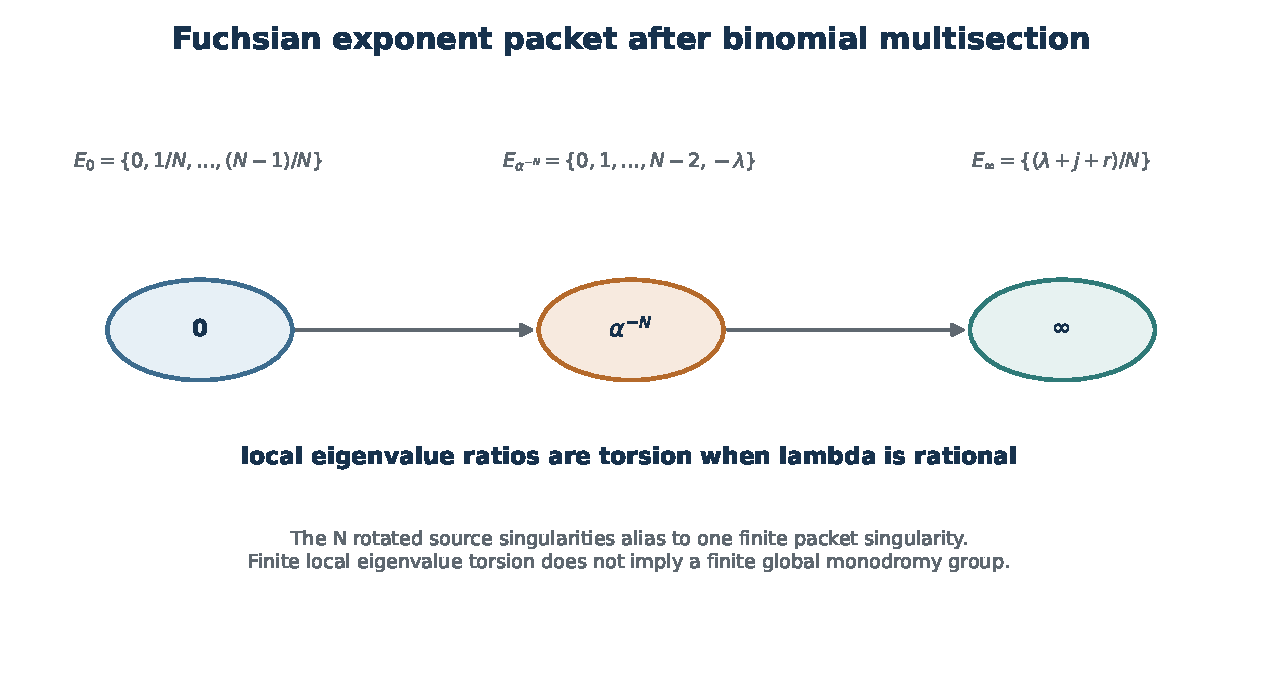
\includegraphics[width=.94\textwidth]{holonomic_exponent_packet.pdf}
\caption{The exact Fuchsian exponent packet of a nonintegral binomial multisection.  Root-orbit aliasing moves $N$ rotated source singularities into one finite singularity while the complete $N$-torsion exponent sets remain visible at zero and infinity.}
\label{fig:block09-exponent-packet}
\end{figure}


\subsection{Marked normalized packet atlas}
\label{subsec:block09-marked-atlas}

The order theorem is most naturally a theorem about marked packets.  Without the mark, distinct choices of source exponent, scale, width, and address can represent the same zero packet or the same rational function.

\begin{definition}[Marked binomial--Fuchsian packet]
\label{def:block09-marked-packet}
A marked packet is a tuple
\[
 \mathfrak b=(\alpha,\lambda,N,j;G),
\]
where $\alpha\neq0$, $N\geq1$, $0\leq j<N$, and
\[
 G(x)=G_{N,j}^{\lambda,\alpha}(x).
\]
The parameters $(\alpha,\lambda,N,j)$ are part of the semantic object rather than metadata to be forgotten.
\end{definition}

For a nonzero marked packet, consider the following normalized charts:
\begin{enumerate}[label=\textup{(\roman*)}]
\item the marked coefficient series $G$;
\item the primitive first-order tail recurrence obtained from the exact coefficient ratio, together with its finite initial record;
\item the monic minimal differential operator from \cref{thm:block09-order-phase}, together with the distinguished power-series solution selected by the marked coefficient record;
\item the hypergeometric parameter packet $\bigl(A_{N,j}(\lambda),B_{N,j};\alpha^N\bigr)$ and leading coefficient;
\item the primitive minimal-operator singular and indicial record
\[
 \mathscr E(G)
 =
 \left(
 \Sigma_{\rm op}(G),
 \bigl(I_{\xi,L_G}\bigr)_{\xi\in\Sigma_{\rm op}(G)}
 \right),
\]
together with the orbit-rank and defect data
\[
 \left(r_{\rm orb},r_D,A_N,C_{N,j}\right).
\]
In the nonintegral Fuchsian regime, \(\mathscr E(G)\) is the explicit three-point packet
\[
 \left(E_0,E_{\alpha^{-N}},E_\infty\right)
\]
computed above.  In the integral regimes it is computed from the corresponding minimal first-order operator.  The zero packets in the terminated regime are retained as separately marked zero objects with the zero-operator convention.
\end{enumerate}

\begin{theorem}[Effective marked binomial--Fuchsian atlas]
\label{thm:block09-marked-descent}
The five normalized presentations above determine one another on the declared marked family.  With equality morphisms they form equivalent discrete groupoids, every normalized fiber is contractible, and objects and morphisms descend effectively.  The package
\[
 \boxed{
 \mathcal J_{\rm BF}
 =
 \left(
 \alpha,\lambda,N,j,
 R_{N,j},L_{N,j},
 A_{N,j}(\lambda),B_{N,j},
 \mathscr E(G),
 r_{\rm orb},r_D,A_N,C_{N,j}
 \right)}
\]
is complete on this marked category.
\end{theorem}

\begin{proof}
The mark constructs the coefficient packet directly.  Consecutive coefficient ratios give the normalized recurrence chart, and the multiplication formula gives the hypergeometric chart.  \Cref{thm:block09-order-phase} identifies the monic minimal differential operator in every parameter regime.  The primitive polynomial representative of that operator determines \(\mathscr E(G)\) by the indicial construction in \cref{subsec:block09-local-exponents}.  In the nonintegral regime, \cref{prop:block09-local-monodromy} gives its explicit Fuchsian eigenvalue ledger.  \Cref{thm:block09-orbit-rank,cor:block09-defect-formulas} compute the orbit and cancellation data in every regime.  Conversely, the displayed invariant retains the complete mark and therefore reconstructs the source packet and every normalized chart.  Uniqueness of monic Ore normalization and of the marked coefficient record leaves no nontrivial automorphism in a fiber.
\end{proof}

\subsection{Examples and exact verification}
\label{subsec:block09-verification}

The parity sections of
\[
 \frac{2}{1-z^2}
\]
give the smallest singularity-alias example.  The source singularities $1$ and $-1$ both map to $1$ under squaring.  The even address is $2/(1-x)$, while the odd address vanishes.

For
\[
 2\cosh z,
\]
the even packet is nonzero and the odd packet is zero.  There is no finite singularity, so the cancellation occurs at the level of the character-projected solution rather than by finite singularity collision.

For the Catalan sequence, every arithmetic section remains hypergeometric in the packet index.  Its recurrence order is one, while its ordinary generating function remains a second-order algebraic D-finite function.  This again shows that recurrence order and scalar differential order are different coordinates.

For the Ap\'ery numbers, the known two-dimensional nonautonomous state jumps to every arithmetic section.  The jump theorem gives an exact order-two recurrence bound, but the present holonomic theorem does not claim a closed minimality formula for all Ap\'ery addresses.

\begin{table}[htbp]
\centering
\small
\caption{Representative exact order profiles in the binomial--Fuchsian packet family.}
\label{tab:block09-examples}
\begin{tabularx}{\textwidth}{@{}L{0.17\textwidth}L{0.13\textwidth}cccccY@{}}
\toprule
Source & Packet & $r_{\rm tail}$ & $r_D$ & $r_{\rm orb}$ & Alias & Cancel & Interpretation\\
\midrule
$(1-z)^{-1/2}$ & $N=2,\ j=0$ & 1 & 2 & 2 & 0 & 0 & irreducible nonintegral packet\\
$(1-z)^{-1/3}$ & $N=3,\ j=2$ & 1 & 3 & 3 & 0 & 0 & finite local exponent torsion\\
$(1-z)^{-2}$ & $N=3,\ j=1$ & 1 & 1 & 3 & 0 & 2 & rational collapse\\
$(1-z)^2$ & $N=4,\ j=1$ & 0 & 1 & 3 & 1 & 2 & finite-support polynomial\\
$(1-z)^2$ & $N=4,\ j=3$ & 0 & 0 & 3 & 1 & 3 & zero address packet\\
\bottomrule
\end{tabularx}
\end{table}

\begin{table}[htbp]
\centering
\caption{Exact Holonomic atlas verification counts.}
\label{tab:block09-validation}
\begin{tabular}{@{}lr@{}}
\toprule
Validation class & Exact checks\\
\midrule
Nonintegral binomial packets & 110,880\\
Positive-integral rational collapse & 27,720\\
Nonpositive-integral aliasing & 11,492\\
Root-filter and order ledger & 24,848\\
\midrule
Holonomic atlas total & 174,940\\
Cumulative the preceding certified atlas program total & 1,838,856\\
Failures & 0\\
\bottomrule
\end{tabular}
\end{table}


The Holonomic atlas verifier checks the binomial packet recurrence, the generalized hypergeometric differential coefficient identity, nonresonance of the irreducible parameter packets, zero and infinity exponent torsion classes, positive-integral rational collapse, nonpositive-integral orbit rank and address support, and root-filter orthogonality.  It records 174,940 exact checks with no failures.

\begin{boundarybox}
\textbf{Exact holonomic boundary.}
The holonomic section proves normalized minimal Ore charts on the ordinary-point locus and an exact multisection minimality theorem for the binomial--Fuchsian packet family.  It does not prove a universal formula for minimal multisection operators of arbitrary D-finite series.  Irregular singularities, Stokes data, apparent-singularity removal, resonant logarithmic extensions, general differential-module cyclicity after character projection, and a finite all-address signature for unrestricted holonomic systems remain open.
\end{boundarybox}

\begin{resultbox}
\textbf{Section result.}
P-recursive and D-finite presentations now form an explicit normalized atlas on the ordinary-point locus, with minimal Ore annihilators, finite prefix and jet certificates, and exact coefficient transport.  General arithmetic multisection has a typed root-filter and state-jump construction, together with an explicit construction-relative minimality defect.  The binomial--Fuchsian family supplies the first exact holonomic packet phase diagram: nonintegral exponents retain differential order $N$, positive integers collapse to rational order one, nonpositive integers terminate with a closed orbit-alias and address-cancellation formula, and the nonintegral local exponent packet exposes the complete finite torsion at zero and infinity.
\end{resultbox}


\section{Selected algebraic branches, packet Weil restriction, and collision invariants}
\label{sec:block10-algebraic}

Algebraic atlas develops the algebraic stratum after the fixed-radix, product, local, and holonomic milestones.  The central issue is not algebraicity alone.  A polynomial equation may have several formal branches, and a packet elimination can contain branch tuples that do not belong to the selected semantic germ.  A normalized algebraic chart must therefore retain both a minimal polynomial and a finite branch selector.  Arithmetic packets are then compiled as a finite polynomial system.  The generic packet scheme is a Weil restriction of the source branch scheme, which gives a uniform degree bound.  A separate collision ledger explains why the degree of one selected packet may be smaller than that bound.

Throughout this section, $K$ is a characteristic-zero field and $\overline K$ is an algebraic closure.  Algebraic degree always means degree over the displayed rational-function field.  All assertions about formal branches are made inside $\overline K[[z]]$ unless a different local field is named.

\subsection{Minimal polynomials and finite branch selectors}
\label{subsec:block10-branch-selector}

Let $F\in K[[z]]$ be algebraic over $K(z)$.  Its monic irreducible polynomial is
\[
 P_F(z,Y)\in K(z)[Y],
 \qquad
 P_F(z,F(z))=0.
\]
Write
\[
 d(F)=\deg_Y P_F.
\]
After multiplying by a common denominator and dividing by the greatest common divisor of the polynomial coefficients, one obtains a primitive representative in $K[z,Y]$, unique up to a nonzero scalar.  We normalize that scalar by fixing the first nonzero coefficient in graded lexicographic order to be one.

A polynomial alone does not select a branch.  Let
\[
 \operatorname{Br}_0(P_F)
 =
 \{G\in\overline K[[z]]:P_F(z,G(z))=0\}.
\]
This set has cardinality at most $d(F)$.

\begin{definition}[Branch-separation index]
For $F\in\operatorname{Br}_0(P_F)$, define
\[
 \sigma(P_F,F)
 =
 \begin{cases}
 0,&\operatorname{Br}_0(P_F)=\{F\},\\[3pt]
 1+\displaystyle\max_{G\in\operatorname{Br}_0(P_F),\,G\neq F}
 \operatorname{ord}_z(F-G),&\text{otherwise}.
 \end{cases}
\]
The corresponding branch selector is the finite coefficient jet
\[
 \boxed{
 J_{\rm alg}(F)
 =
 (a_0,a_1,\ldots,a_{\sigma-1}),
 \qquad
 F(z)=\sum_{n\geq0}a_nz^n.}
\]
When $\sigma=0$, the selector is empty.
\end{definition}

\begin{theorem}[Finite branch separation]
\label{thm:block10-finite-branch-separation}
The pair
\[
 \boxed{(P_F,J_{\rm alg}(F))}
\]
selects $F$ uniquely among the formal power-series branches of $P_F$ at the origin.
\end{theorem}

\begin{proof}
There are at most $d(F)$ formal branches.  The difference of two distinct formal series has finite $z$-adic order.  By definition of $\sigma$, every other branch differs from $F$ in one of the coefficients recorded by $J_{\rm alg}(F)$.
\end{proof}

The simplest case is the ordinary implicit-function locus.

\begin{corollary}[Simple-branch normalization]
\label{cor:block10-simple-branch}
If
\[
 P_F(0,a_0)=0,
 \qquad
 \partial_Y P_F(0,a_0)\neq0,
\]
then $a_0$ alone selects a unique formal branch.  Equivalently, $\sigma(P_F,F)\leq1$.
\end{corollary}

\begin{proof}
Coefficient comparison in $P_F(z,F(z))=0$ determines each next coefficient linearly, with diagonal coefficient $\partial_Y P_F(0,a_0)$.
\end{proof}

The finite selector is semantic data.  It cannot be dropped merely because the polynomial is irreducible over $K(z)$.  Irreducibility controls the generic function-field extension, while the jet chooses one local embedding of that extension into formal series.

\subsection{The normalized selected-branch atlas}
\label{subsec:block10-branch-atlas}

Let
\[
 A_F=K(z)[Y]/(P_F),
\]
and let $\bar Y$ denote the residue class of $Y$.  In the basis
\[
 1,\bar Y,\ldots,\bar Y^{d-1},
\]
multiplication by $\bar Y$ is represented by the companion matrix $M_F$.  Its characteristic and minimal polynomials are both $P_F$.

\begin{theorem}[Normalized selected-branch algebraic atlas]
\label{thm:block10-branch-atlas}
The following normalized presentations determine one another exactly:
\[
 \boxed{
 \begin{aligned}
 &F\in K[[z]],\\
 &(P_F,J_{\rm alg}(F)),\\
 &(A_F,\bar Y,J_{\rm alg}(F)),\\
 &(M_F,J_{\rm alg}(F)).
 \end{aligned}}
\]
With equality morphisms, these presentations form equivalent normalized groupoids.  Every fiber over a fixed semantic branch is contractible.
\end{theorem}

\begin{proof}
The semantic branch gives its unique monic minimal polynomial and its finite branch selector.  The polynomial gives the finite field algebra and its companion multiplication matrix.  Conversely, the companion matrix recovers $P_F$ as its minimal polynomial.  The branch selector then recovers the selected formal root by \cref{thm:block10-finite-branch-separation}.  Every normalized presentation is determined literally, so a normalized automorphism fixing the semantic branch is the identity.
\end{proof}

\begin{figure}[htbp]
\centering
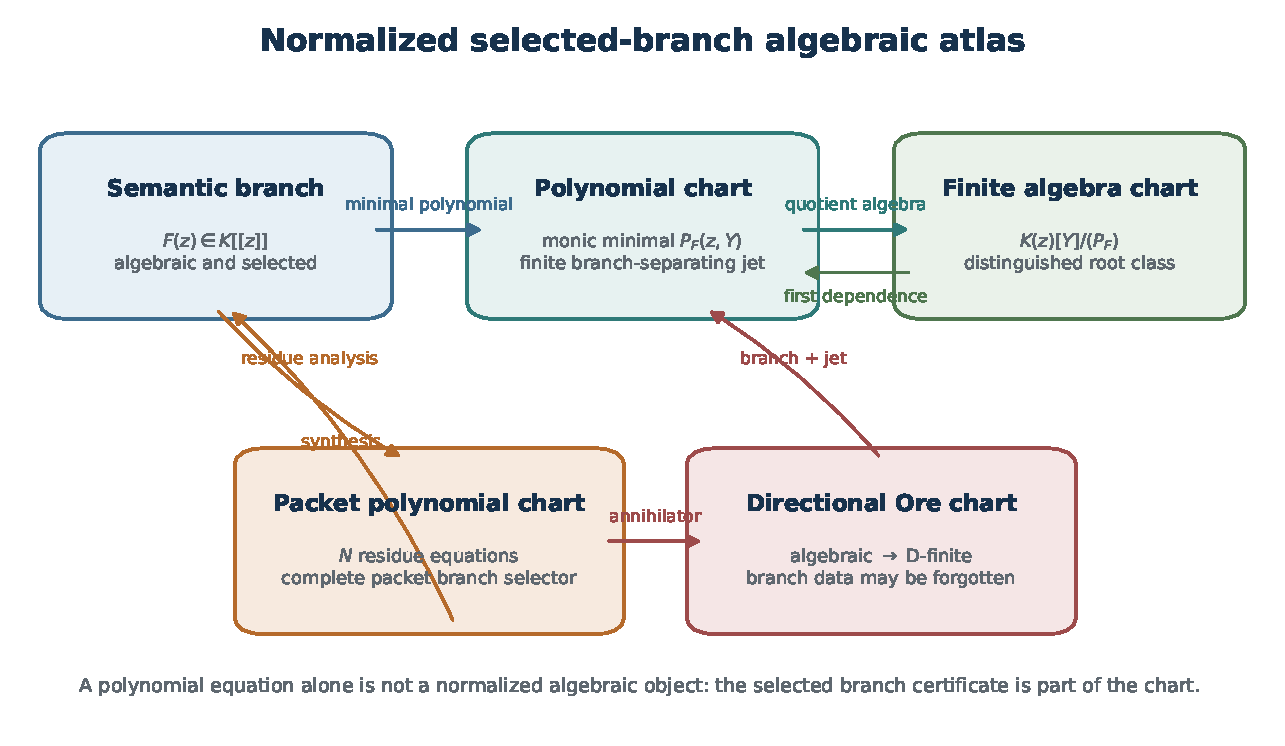
\includegraphics[width=.98\textwidth]{algebraic_branch_atlas.pdf}
\caption{The selected algebraic branch, its minimal polynomial and finite selector, its finite quotient algebra, and its complete packet system are reversible normalized charts.  The Ore chart is directional because an annihilator can forget branch data.}
\label{fig:block10-branch-atlas}
\end{figure}

\subsection{The exact residue-packet polynomial compiler}
\label{subsec:block10-packet-compiler}

Fix $N\geq1$.  For
\[
 F(z)=\sum_{n\geq0}a_nz^n,
\]
define the arithmetic packets
\[
 U_j(x)
 =
 \sum_{m\geq0}a_{Nm+j}x^m,
 \qquad
 0\leq j<N.
\]
They satisfy the exact synthesis identity
\[
 \boxed{
 F(z)
 =
 \sum_{j=0}^{N-1}z^jU_j(z^N).}
\]

Let $P(z,Y)\in K[z,Y]$ be the normalized primitive representative of $P_F$.  Introduce indeterminates
\[
 \mathbf U=(U_0,\ldots,U_{N-1})
\]
and substitute
\[
 Y=\sum_{j=0}^{N-1}z^jU_j.
\]
Every polynomial in $z$ has a unique decomposition modulo the relation $z^N=x$:
\[
 P\!\left(z,\sum_{j=0}^{N-1}z^jU_j\right)
 =
 \sum_{r=0}^{N-1}z^r\Phi_{N,r}(x,\mathbf U).
\]
The polynomials
\[
 \boxed{
 \Phi_{N,r}(x,\mathbf U)\in K[x,\mathbf U]}
\]
are the algebraic packet equations.

\begin{theorem}[Exact algebraic packet system]
\label{thm:block10-exact-packet-system}
Let $d=\deg_Y P_F$.  Then:
\begin{enumerate}
\item the semantic packet tuple $(U_0,\ldots,U_{N-1})$ satisfies
\[
 \Phi_{N,r}(x,\mathbf U)=0
 \qquad(0\leq r<N);
\]
\item every $\Phi_{N,r}$ has total degree at most $d$ in the packet variables;
\item a formal packet tuple satisfying all $N$ equations synthesizes a formal branch of $P_F$;
\item the packet tuple selected by the transported coefficient jet reconstructs $F$ uniquely.
\end{enumerate}
\end{theorem}

\begin{proof}
Substituting the semantic synthesis formula into $P_F(z,F(z))=0$ gives the first statement.  Substitution does not increase degree in the $U_j$, so the second follows.  If all residue polynomials vanish, then the synthesized series satisfies $P_F=0$.  The source branch selector is distributed among the packets by residue class.  The resulting packet jet synthesizes the original jet, so \cref{thm:block10-finite-branch-separation} identifies the selected branch.
\end{proof}

If the source selector records $a_0,\ldots,a_{\sigma-1}$, the transported packet selector records precisely
\[
 [x^m]U_j=a_{Nm+j}
 \qquad
 \text{for }Nm+j<\sigma.
\]
No information is added or lost.  The coefficient prefix is merely rewritten in packet addresses.

\subsection{Weil-restricted packet degree}
\label{subsec:block10-weil-degree}

Put
\[
 R=K(x),
 \qquad
 E_N=R[z]/(z^N-x).
\]
Characteristic zero makes $z^N-x$ separable over $R$.  Interpret the monic polynomial $P_F(z,Y)$ as a polynomial in $E_N[Y]$, and define
\[
 B_{N,F}=E_N[Y]/(P_F).
\]
The packet polynomial system is the coordinate presentation of the finite Weil restriction
\[
 \operatorname{Res}_{E_N/R}\operatorname{Spec}B_{N,F}.
\]

\begin{theorem}[Algebraic packet degree bound]
\label{thm:block10-packet-degree-bound}
Let $F$ have algebraic degree $d$ over $K(z)$.  For every packet width $N$:
\begin{enumerate}
\item the generic geometric degree of the complete packet scheme is
\[
 \boxed{d^N;}
\]
\item the joint field generated by a selected complete packet satisfies
\[
 \boxed{
 [K(x)(U_0,\ldots,U_{N-1}):K(x)]\leq d^N;}
\]
\item every individual packet satisfies
\[
 \boxed{
 [K(x)(U_j):K(x)]\leq d^N.}
\]
\end{enumerate}
\end{theorem}

\begin{proof}
Over an algebraic closure of $K(x)$, the equation $z^N=x$ has $N$ distinct roots.  The algebra $E_N$ therefore splits into a product of $N$ copies of the algebraic closure.  At each address, the separable degree-$d$ polynomial $P_F$ has $d$ geometric roots.  The Weil-restricted fiber is their Cartesian product and has $d^N$ points.  A selected packet tuple is one point of this finite scheme, so its residue field and every coordinate subfield have degree at most the scheme degree.
\end{proof}

This bound is constructive.  The quotient of
\[
 K(x)[U_0,\ldots,U_{N-1}]
\]
by the packet equations is a finite algebra of generic rank $d^N$.  Multiplication by $U_j$ is therefore a matrix of size $d^N$.  Its characteristic polynomial annihilates $U_j$ by Cayley--Hamilton.

\begin{corollary}[Constructive packet eliminant]
\label{cor:block10-constructive-eliminant}
For each $j$, one can compute an annihilating polynomial
\[
 Q_{N,j}(x,T)\in K(x)[T]
\]
with
\[
 \deg_TQ_{N,j}\leq d^N
\]
by multiplication matrices, resultants, or a Gr\"obner elimination of the exact packet system.
\end{corollary}

The bound is a universal degree ceiling for the minimal-polynomial grammar.  It does not assert that every coordinate attains degree $d^N$ or that one elimination algorithm returns the minimal polynomial without factor selection.

\begin{figure}[htbp]
\centering
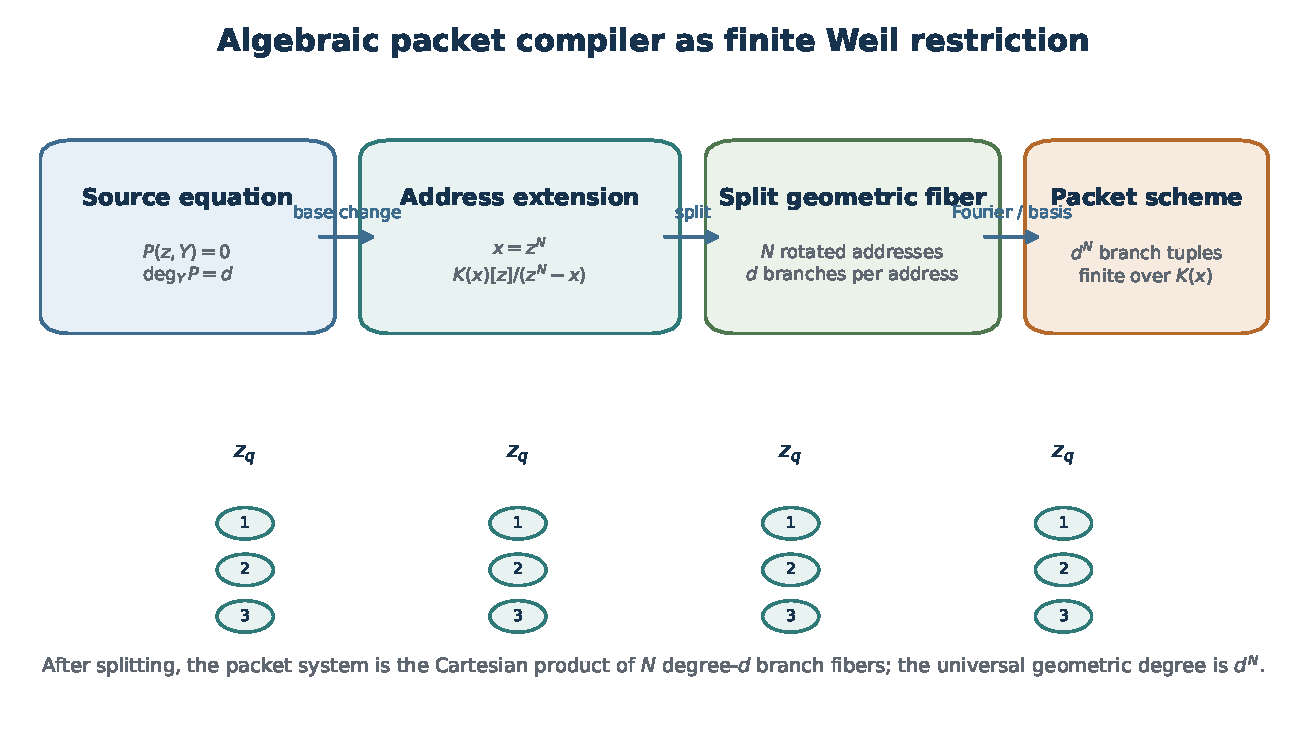
\includegraphics[width=.98\textwidth]{algebraic_packet_weil_restriction.pdf}
\caption{After the address extension $x=z^N$ splits, each of the $N$ addresses carries $d$ algebraic branches.  The complete packet scheme is their Cartesian product and has generic degree $d^N$.}
\label{fig:block10-weil-restriction}
\end{figure}

\subsection{Tuple collision and selected-orbit loss}
\label{subsec:block10-collision-ledger}

Let $\Omega$ be a normal splitting field of the generic packet scheme over $K(x)$, and let
\[
 \Gamma=\operatorname{Gal}(\Omega/K(x)).
\]
After splitting $E_N$, the geometric packet branches form a set
\[
 \mathcal B_N
\]
of cardinality $d^N$.  Let
\[
 \pi_j:\mathcal B_N\to\Omega
\]
be the $j$th packet coordinate, and set
\[
 \mathcal C_{N,j}=\pi_j(\mathcal B_N).
\]
For the selected semantic packet $U_j$, separability gives
\[
 [K(x)(U_j):K(x)]
 =
 |\Gamma\cdot U_j|.
\]

\begin{definition}[Algebraic packet collision defects]
Define
\[
 \mathfrak c^{\rm tuple}_{N,j}
 =
 d^N-|\mathcal C_{N,j}|,
\]
and
\[
 \mathfrak s^{\rm Gal}_{N,j}
 =
 |\mathcal C_{N,j}|-|\Gamma\cdot U_j|.
\]
The first records collisions caused by projection from complete branch tuples to one packet coordinate.  The second records the remaining loss caused by the Galois stabilizer of the selected coordinate.
\end{definition}

\begin{theorem}[Exact algebraic degree-defect identity]
\label{thm:block10-degree-defect}
The two defects are nonnegative and satisfy
\[
 \boxed{
 d^N-[K(x)(U_j):K(x)]
 =
 \mathfrak c^{\rm tuple}_{N,j}
 +
 \mathfrak s^{\rm Gal}_{N,j}.}
\]
\end{theorem}

\begin{proof}
The coordinate image $\mathcal C_{N,j}$ has at most $d^N$ values.  The Galois orbit of the selected value is contained in that image.  The displayed identity is the telescoping decomposition
\[
 d^N-|\Gamma\cdot U_j|
 =
 (d^N-|\mathcal C_{N,j}|)
 +
 (|\mathcal C_{N,j}|-|\Gamma\cdot U_j|).
\]
\end{proof}

This signature separates two mechanisms that a raw resultant merges.  Repeated projected values are a coordinate collision.  A smaller selected orbit is a descent or stabilizer phenomenon.  They are not the same obstruction.

\begin{figure}[htbp]
\centering
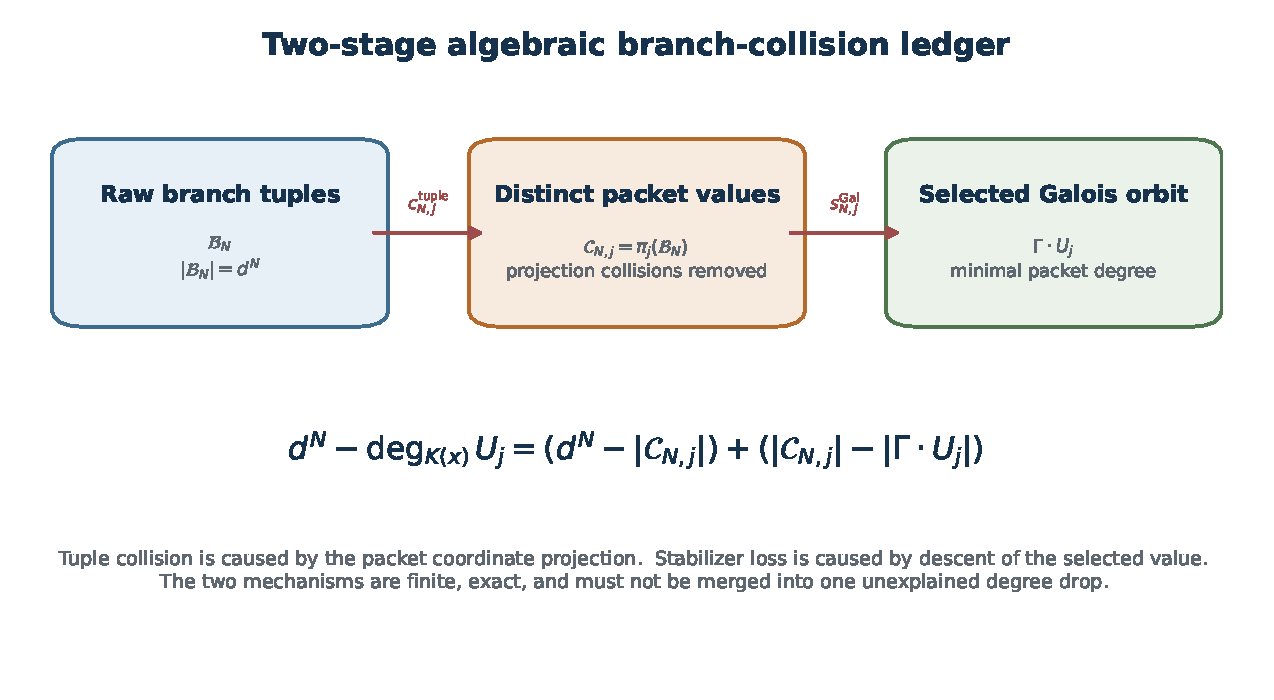
\includegraphics[width=.96\textwidth]{algebraic_collision_defects.pdf}
\caption{The universal degree $d^N$ can drop first because several branch tuples have the same packet coordinate, then because the selected coordinate has a nontrivial Galois stabilizer.}
\label{fig:block10-collision-ledger}
\end{figure}

\subsection{A sharp Catalan parity theorem}
\label{subsec:block10-catalan}

Let
\[
 C(z)=1+zC(z)^2
\]
be the Catalan branch with $C(0)=1$, and write
\[
 C(z)=E(z^2)+zO(z^2).
\]
Put $x=z^2$.

\begin{theorem}[Exact Catalan packet system]
\label{thm:block10-catalan-system}
The parity packets satisfy
\[
 \boxed{
 E=1+2xEO,
 \qquad
 O=E^2+xO^2.}
\]
Elimination gives
\[
 \boxed{4xE^4-E^2+1=0}
\]
and
\[
 \boxed{4x^3O^4-8x^2O^3+5xO^2-O+1=0.}
\]
Both packets have algebraic degree four over $K(x)$.  Hence the universal bound
\[
 d^N=2^2=4
\]
is sharp.
\end{theorem}

\begin{proof}
Substitute $C=E+zO$ into $C=1+zC^2$ and separate even and odd powers.  The two resultants give the displayed quartics.

For the even packet, put $T=E^2$.  Then
\[
 4xT^2-T+1=0.
\]
Its discriminant $1-16x$ is not a square in $K(x)$, so $[K(x)(T):K(x)]=2$.  The norm of $T$ from this quadratic field is $1/(4x)$, which is not a square in $K(x)$.  Therefore $T$ is not a square in its quadratic field and $E$ has degree four.

The first packet equation gives
\[
 O=\frac{E-1}{2xE},
 \qquad
 E=\frac{1}{1-2xO}.
\]
Thus $K(x)(E)=K(x)(O)$, and the odd packet also has degree four.
\end{proof}

The Catalan parity packet has no tuple-collision or selected-orbit defect.  Its one-coordinate degree already sees all four geometric branch tuples of the quadratic source over the two addresses.

\subsection{A quadratic-radical collision phase diagram}
\label{subsec:block10-quadratic-radical}

Let
\[
 F_{\alpha,\beta}(z)
 =
 \sqrt{(1-\alpha z)(1-\beta z)},
 \qquad
 F_{\alpha,\beta}(0)=1,
\]
and assume first that $\alpha\neq\beta$, so the normalized source degree is two.  Write
\[
 F_{\alpha,\beta}(z)=E(x)+zO(x),
 \qquad
 x=z^2,
\]
and put
\[
 s=\alpha+\beta,
 \qquad
 p=\alpha\beta.
\]

\begin{theorem}[Quadratic-radical parity packets]
\label{thm:block10-radical-packets}
The packets satisfy
\[
 \boxed{
 E^2+xO^2=1+px,
 \qquad
 2EO=-s.}
\]
Their eliminants are
\[
 \boxed{
 E^4-(1+px)E^2+\frac{s^2x}{4}=0}
\]
and
\[
 \boxed{
 xO^4-(1+px)O^2+\frac{s^2}{4}=0.}
\]
If
\[
 s\neq0,
 \qquad
 \alpha^2\neq\beta^2,
\]
then both selected packets have degree four over $K(x)$.
\end{theorem}

\begin{proof}
The two equations follow by adding and subtracting the squares of
\[
 F(z)=E+zO,
 \qquad
 F(-z)=E-zO.
\]
Elimination gives the quartics.  Their quadratic discriminant is
\[
 \Delta(x)
 =
 (1-\alpha^2x)(1-\beta^2x),
\]
which is not a square under the stated hypotheses.  Hence $E^2$ generates a quadratic extension.  Its norm is $s^2x/4$, which is not a square in $K(x)$, so $E$ has degree four.  Since $EO=-s/2$, the fields generated by $E$ and $O$ coincide.
\end{proof}

The symmetric case produces an exact collision.

\begin{corollary}[Antisymmetric branch collision]
\label{cor:block10-antisymmetric-collision}
If $\beta=-\alpha\neq0$, then
\[
 \boxed{O=0,
 \qquad
 E^2=1-\alpha^2x.}
\]
For the even coordinate,
\[
 |\mathcal B_2|=4,
 \qquad
 |\mathcal C_{2,0}|=3,
 \qquad
 |\Gamma\cdot E|=2.
\]
Thus
\[
 \mathfrak c^{\rm tuple}_{2,0}=1,
 \qquad
 \mathfrak s^{\rm Gal}_{2,0}=1.
\]
For the selected odd coordinate,
\[
 |\mathcal C_{2,1}|=3,
 \qquad
 |\Gamma\cdot O|=1,
\]
so
\[
 \mathfrak c^{\rm tuple}_{2,1}=1,
 \qquad
 \mathfrak s^{\rm Gal}_{2,1}=2.
\]
\end{corollary}

\begin{proof}
Now $F(z)=F(-z)=\sqrt{1-\alpha^2z^2}$ for the selected branch, so the odd packet vanishes.  Over the split branch tuple set, the two signs are chosen independently.  The even projection has values $E,0,-E$, while the odd projection has values $0,E/z,-E/z$.  The selected Galois orbits have sizes two and one, respectively.
\end{proof}

If $\alpha=\beta$, the quadratic equation
\[
 Y^2-(1-\alpha z)^2=0
\]
is not the normalized source polynomial.  The selected branch is rational:
\[
 F_{\alpha,\alpha}(z)=1-\alpha z,
\]
so the correct source degree is one.  This is a negative control against using a nonminimal defining equation in the degree ledger.

\begin{figure}[htbp]
\centering
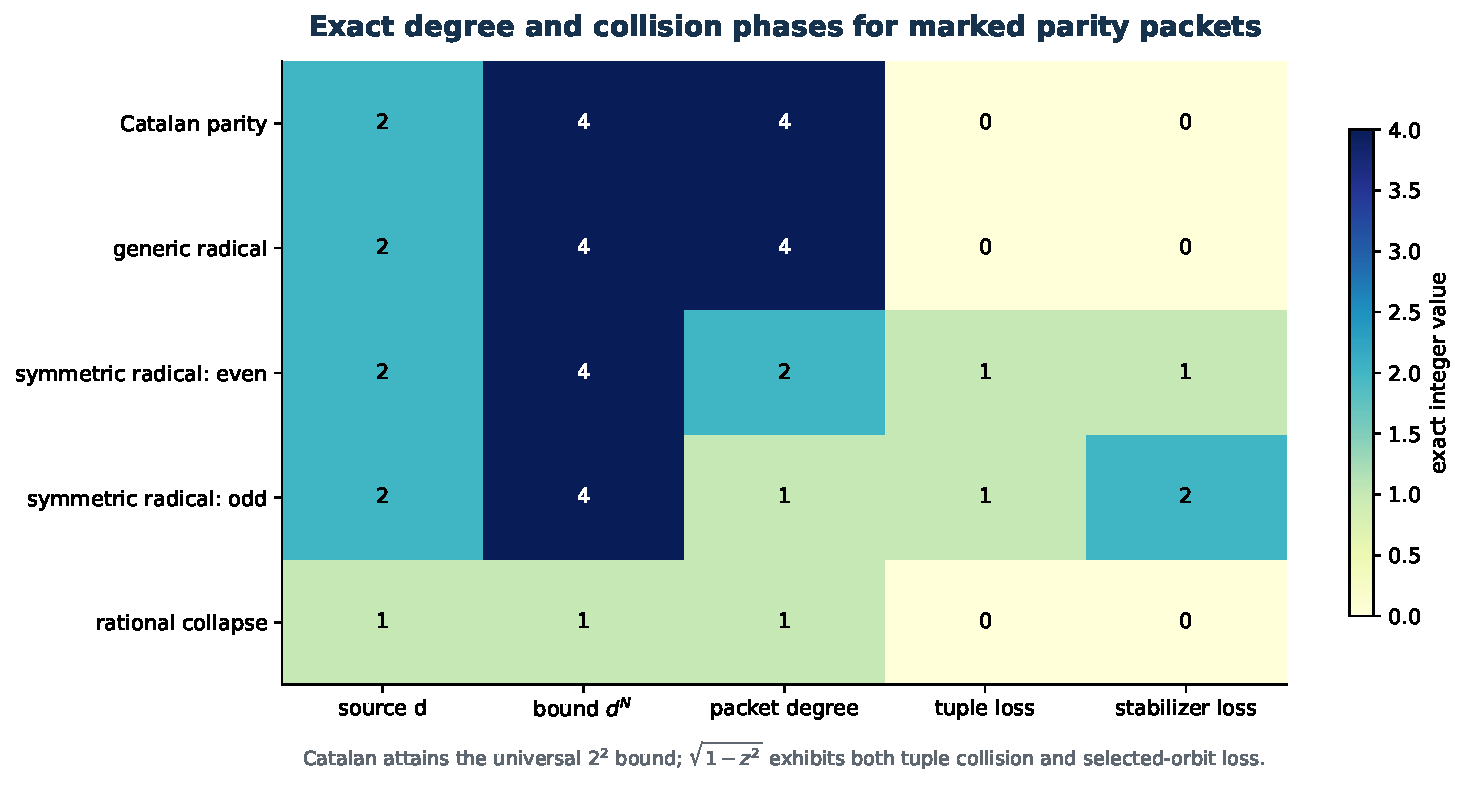
\includegraphics[width=.98\textwidth]{algebraic_quadratic_phase.pdf}
\caption{Catalan parity packets attain the universal quadratic bound.  Generic radicals do the same, while the antisymmetric radical separates tuple collision from selected-orbit loss.  A repeated linear factor must first be reduced to its minimal source polynomial.}
\label{fig:block10-quadratic-phase}
\end{figure}

\subsection{The directional algebraic-to-holonomic bridge}
\label{subsec:block10-algebraic-holonomic}

Algebraic functions are D-finite, but this bridge is directional unless branch data is retained.

\begin{proposition}[Algebraic derivative closure]
\label{prop:block10-algebraic-dfinite}
Let $F$ have separable minimal polynomial $P_F$ of degree $d$.  Then
\[
 F'
 =
 -\frac{\partial_zP_F(z,F)}{\partial_YP_F(z,F)}
 \in
 K(z,F).
\]
Every higher derivative lies in the same degree-$d$ function field.  Consequently, $F$ has a differential annihilator of order at most $d$.
\end{proposition}

\begin{proof}
Differentiate $P_F(z,F(z))=0$.  Separability makes $\partial_YP_F(z,F)$ nonzero in the function field.  The field is closed under the induced derivation.  The $d+1$ elements $F,F',\ldots,F^{(d)}$ are linearly dependent over $K(z)$.
\end{proof}

The annihilator can forget both the polynomial relation and the selected branch.  For example,
\[
 \sqrt{1+z}
 \quad\text{and}\quad
 -\sqrt{1+z}
\]
satisfy the same first-order differential operator.  Their initial values distinguish them.  More generally, a D-finite equation may have transcendental solutions, so an Ore chart does not reconstruct an algebraic minimal polynomial without additional recognition data.

\begin{boundarybox}
\textbf{Exact algebraic boundary.}
Algebraic atlas proves finite selected-branch normalization, an exact packet polynomial compiler, the generic $d^N$ Weil-restriction degree, a constructive coordinate eliminant, and a two-stage collision invariant.  It proves sharp packet degrees for Catalan parity and a complete collision phase for a marked quadratic-radical family.  It does not prove that every elimination output is minimal without factor selection, one canonical minimal polynomial-system dimension across arbitrary multivariate grammars, an optimal packet-degree bound using all source symmetries, or unrestricted equivalence between algebraic and D-finite presentations.
\end{boundarybox}

\subsection{Exact examples and finite verification}
\label{subsec:block10-verification}

The verifier independently constructs packet equations by substitution and reduction modulo $z^N=x$.  It checks Catalan, Motzkin, and marked radical branches at several packet widths.  It verifies the sharp Catalan quartics, the quadratic-radical trace and norm systems, the generic and antisymmetric collision phases, the rejection of nonminimal quadratic equations, and finite branch-selector certificates.

\begin{resultbox}
\textbf{Section result.}
A selected algebraic branch has a canonical minimal polynomial and a finite branch-separating jet.  Complete arithmetic packets are the solutions of an explicit $N$-equation polynomial system obtained by residue reduction.  The generic packet scheme is a finite Weil restriction of degree $d^N$, giving a constructive degree bound for every packet coordinate.  Degree loss splits exactly into tuple projection collisions and Galois stabilizer loss.  Catalan parity attains the universal quadratic bound, while the marked radical family exhibits generic sharpness, antisymmetric cancellation, and rational collapse.  The algebraic-to-holonomic bridge remains directional unless the minimal polynomial and branch selector are retained.
\end{resultbox}

\begin{table}[H]
\centering
\scriptsize
\caption{Representative exact degree and collision profiles in the Algebraic atlas algebraic packet atlas.}
\label{tab:block10-examples}
\begin{tabularx}{\textwidth}{@{}L{0.17\textwidth}L{0.14\textwidth}cccccY@{}}
\toprule
Source & Packet & $d$ & $d^N$ & degree & tuple loss & stabilizer loss & Interpretation\\
\midrule
$C=1+zC^2$ & parity $(E,O)$ & 2 & 4 & 4 & 0 & 0 & sharp Weil-restriction bound\\
$\sqrt{(1-z)(1-2z)}$ & parity even/odd & 2 & 4 & 4 & 0 & 0 & generic biquadratic packet\\
$\sqrt{1-z^2}$ & even packet & 2 & 4 & 2 & 1 & 1 & rotation alias plus descent stabilizer\\
$\sqrt{1-z^2}$ & odd packet & 2 & 4 & 1 & 1 & 2 & exact zero-address cancellation\\
$\sqrt{(1-z)^2}=1-z$ & normalized source & 1 & 1 & 1 & 0 & 0 & nonminimal quadratic equation rejected\\
\bottomrule
\end{tabularx}
\end{table}

\begin{table}[H]
\centering
\small
\caption{Exact finite validation of the Algebraic atlas algebraic packet layer.}
\label{tab:block10-validation}
\begin{tabularx}{\textwidth}{@{}L{0.34\textwidth}rY@{}}
\toprule
Validation class & Checks & Scope\\
\midrule
General Packet Compiler & 3,690 & Catalan, Motzkin, and marked quadratic radicals at packet widths two through four\\
Catalan Sharp Parity & 7,426 & exact parity system, quartic eliminants, and irreducibility ledger\\
Quadratic Radical Collision Phase & 43,900 & generic degree four, antisymmetric cancellation, and rational collapse\\
Finite Branch Selectors & 16,632 & finite jets separating explicitly colliding formal branches\\
Collision Ledger Combinatorics & 1,440 & finite tuple-collision and selected-orbit defect identities\\
\midrule
\textbf{Algebraic atlas total} & \textbf{73,088} & \textbf{0 failures}\\
Cumulative the preceding certified atlas program & 1,911,944 & frozen prior records plus recomputed Algebraic atlas\\
\bottomrule
\end{tabularx}
\end{table}




\section{Nonlinear polynomial fixed points, compressed packet composition, and finite tree signatures}
\label{sec:block11-nonlinear-tree}

Nonlinear tree atlas develops the nonlinear and rooted-tree stratum after the algebraic milestone.  The existing nonlinear sources already prove exact packet jets, the packet Fa\`a di Bruno law, colored operadic composition, refinement coherence, rooted-tree reconstruction, analytic majorant estimates, and local near-identity inversion \cite{P3,RT,NLO}.  The remaining problem is not whether nonlinear maps can be expanded.  It is whether a declared nonlinear family admits a normalized finite presentation and a finite signature that controls a named packet complexity.

This section gives three restricted answers.  First, a marked polynomial fixed-point system is organized into equivalent system, packet-hypergraph, operadic-tree, and exact packet-equation charts.  Second, repeated-direction packet Fa\`a di Bruno sums admit an exact orbit compression indexed by colored integer partitions rather than all labeled set partitions.  Third, simply generated plane-tree equations possess a finite arity-gcd signature that determines every packet-support pattern and, under the classical smooth implicit schema, the complete dominant-singularity orbit after arithmetic packetization.  A dependency condensation isolates the exact cyclic nonlinear core of a marked packet system.  None of these results is promoted to a universal nonlinear normal form.

Throughout the analytic part, $X$ is a Banach space over $\mathbb R$ or $\mathbb C$.  A finite packet system on $X$ is a family of bounded projections
\[
 P_iP_j=\delta_{ij}P_i,
 \qquad
 \sum_{i\in I}P_i=I_X.
\]
All sums over packet addresses are finite.  The formal-series part is valid over any characteristic-zero field unless positivity or singularity analysis is explicitly invoked.

\subsection{Marked polynomial fixed-point systems}
\label{subsec:block11-marked-systems}

Let
\[
 A_m:X^m\longrightarrow X,
 \qquad 2\le m\le D,
\]
be bounded symmetric multilinear maps, and let $s\in X$.  Consider the marked equation
\[
 \boxed{
 u=s+\Phi(u),
 \qquad
 \Phi(u)=\sum_{m=2}^{D}A_m[u,\ldots,u].}
 \tag{11.1}
\]
The word \emph{marked} means that the source term, every multilinear operation, the packet system, and the selected convergence or filtration certificate are retained as part of the presentation.  The fixed point $u$ alone is not assumed to reconstruct those data.

Put
\[
 a=\lVert s\rVert,
 \qquad
 b_m=\lVert A_m\rVert,
 \qquad
 \varphi(t)=\sum_{m=2}^{D}b_mt^m.
\]
For a radius $R>0$, define
\[
 \kappa_R=\varphi'(R)
 =\sum_{m=2}^{D}m b_mR^{m-1}.
\]

\begin{theorem}[Selected polynomial fixed point and tree expansion]
\label{thm:block11-polynomial-fixed-point}
Assume
\[
 a+\varphi(R)\le R,
 \qquad
 \kappa_R<1.
\]
Then equation \textup{(11.1)} has a unique solution in the closed ball $\overline B_R$.  Moreover, that solution is the absolutely convergent sum
\[
 \boxed{
 u=\sum_{T\in\mathcal T_{\mathcal A}}\operatorname{ev}(T),}
 \tag{11.2}
\]
where $\mathcal A=\{m:A_m\neq0\}$, the leaves of $T$ evaluate to $s$, and an internal vertex of arity $m$ evaluates by $A_m$ applied to the ordered values of its children.
\end{theorem}

\begin{proof}
The map
\[
 \Psi(x)=s+\Phi(x)
\]
preserves $\overline B_R$ because
\[
 \lVert\Psi(x)\rVert
 \le a+\sum_{m=2}^{D}b_mR^m
 \le R.
\]
For $x,y\in\overline B_R$, multilinearity gives
\[
 A_m[x^m]-A_m[y^m]
 =
 \sum_{r=1}^{m}
 A_m[y^{r-1},x-y,x^{m-r}],
\]
so
\[
 \lVert\Psi(x)-\Psi(y)\rVert
 \le
 \kappa_R\lVert x-y\rVert.
\]
The contraction theorem gives the unique fixed point.

Let $u^{(0)}=0$ and $u^{(h+1)}=\Psi(u^{(h)})$.  Expanding recursively shows that $u^{(h)}$ is the sum of the evaluations of all allowed plane rooted trees of height at most $h-1$.  If $r_0=0$ and
\[
 r_{h+1}=a+\varphi(r_h),
\]
then the sum of the norms of those tree evaluations is at most $r_h$.  The scalar iterates increase and remain bounded by $R$, hence converge.  Monotone convergence of the nonnegative norm majorant proves absolute convergence of the full tree sum.  Regrouping trees by the arity of the root gives equation \textup{(11.1)}.
\end{proof}

\begin{remark}[Formal filtered version]
If $X$ is replaced by a complete filtered module, $s$ begins in positive filtration, and every $A_m$ raises total filtration, then the same tree expansion is coefficientwise finite at each filtration depth.  It therefore defines the unique formal solution without a Banach norm.  The analytic and formal doctrines are related but are not silently identified.
\end{remark}

\begin{boundary}[The selected object is a marked system]
Two different polynomial systems can have the same fixed point.  Conversely, a single polynomial system can have several fixed points outside the contraction ball.  The normalized object in this section is therefore
\[
 (s,A_2,\ldots,A_D;\mathcal P;\text{certificate}),
\]
not an unmarked semantic vector $u$.
\end{boundary}

\subsection{Packet jets, hypergraphs, and the marked nonlinear atlas}
\label{subsec:block11-packet-atlas}

For $i,j_1,\ldots,j_m\in I$, define the resolved multilinear block
\[
 A_{m;i\mid j_1,\ldots,j_m}
 =
 P_iA_m(P_{j_1}\,\cdot,\ldots,P_{j_m}\,\cdot).
\]
Completeness of the packet family gives the exact reconstruction
\[
 \boxed{
 A_m
 =
 \sum_{i,j_1,\ldots,j_m}
 A_{m;i\mid j_1,\ldots,j_m}.}
 \tag{11.3}
\]
Write
\[
 u_i=P_iu,
 \qquad
 s_i=P_is.
\]
Then equation \textup{(11.1)} is equivalent to the complete packet system
\[
 \boxed{
 u_i
 =
 s_i+
 \sum_{m=2}^{D}
 \sum_{j_1,\ldots,j_m}
 A_{m;i\mid j_1,\ldots,j_m}
 [u_{j_1},\ldots,u_{j_m}].}
 \tag{11.4}
\]

The active nonlinear transfer hypergraph has packet addresses as colors and one typed hyperedge
\[
 (j_1,\ldots,j_m)\longrightarrow i
\]
for every nonzero block $A_{m;i\mid j_1,\ldots,j_m}$.  Rooted substitution of these hyperedges is precisely the colored symmetric operad already present in the nonlinear core sources \cite{RT,NLO}.

\begin{theorem}[Normalized atlas of a marked polynomial system]
\label{thm:block11-marked-atlas}
Fix a finite packet system and a certificate satisfying the hypotheses of \cref{thm:block11-polynomial-fixed-point}, or a declared complete filtration satisfying the formal version.  The following presentations determine one another exactly:
\[
 \boxed{
 \begin{aligned}
 &\text{the marked polynomial system }(s,A_2,\ldots,A_D),\\
 &\text{the complete family of packet blocks }A_{m;i\mid j_1,\ldots,j_m},\\
 &\text{the colored operadic tree grammar with its actual vertex operations},\\
 &\text{the exact packet fixed-point system \textup{(11.4)}}.
 \end{aligned}}
\]
Each chart reconstructs the same selected fixed point.  With literal normalized data and equality morphisms, every semantic fiber is contractible.
\end{theorem}

\begin{proof}
Equation \textup{(11.3)} reconstructs each multilinear operation from its complete block family.  The active hypergraph together with the actual block maps is simply another indexing of the same data.  Rooted operadic substitution generates exactly the tree evaluations of \cref{thm:block11-polynomial-fixed-point}.  Applying the output projections to the fixed-point equation gives \textup{(11.4)}, and synthesis recovers the original equation.  Once the packet system, block maps, source term, and certificate are normalized literally, an automorphism fixing the semantic object and all marked data is the identity.
\end{proof}

\begin{figure}[htbp]
\centering
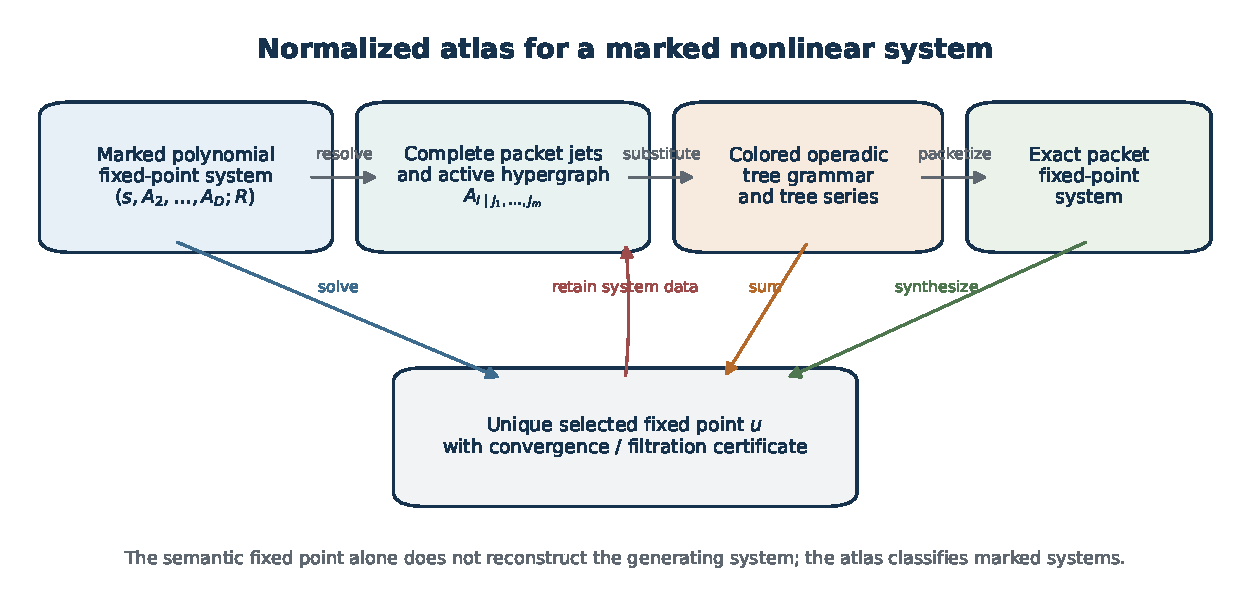
\includegraphics[width=.98\textwidth]{nonlinear_marked_atlas.pdf}
\caption{The marked system, its complete packet jets, its operation-labeled tree grammar, and its exact packet equations are reversible charts.  The fixed point by itself is directional because it forgets the generating system.}
\label{fig:block11-marked-atlas}
\end{figure}

\subsection{Exact diagonal packet Fa\`a di Bruno compression}
\label{subsec:block11-faa-compression}

The packet Fa\`a di Bruno theorem from the nonlinear source expands an $n$th derivative over all set partitions and all intermediate packet labels \cite{P3,RT,NLO}.  When all directions are equal, the symmetric derivative tensors make many labeled terms identical.  They can be grouped exactly by block-size and packet-color multiplicities.

Let $F:Y\to Z$ and $G:X\to Y$ be $n$ times differentiable.  Fix an input packet $\beta$, an output packet $\delta$, a point $x$, and a direction $h\in P_\beta X$.  For every intermediate packet $\gamma$ and every $r\ge1$, put
\[
 g_{r,\gamma}
 =
 Q_\gamma D^rG(x)[h,\ldots,h].
\]
A colored partition profile is a finite family
\[
 \mu=(\mu_{r,\gamma})_{r\ge1,\,\gamma\in\Gamma}
\]
of nonnegative integers satisfying
\[
 \sum_{r,\gamma}r\mu_{r,\gamma}=n.
\]
Let
\[
 k(\mu)=\sum_{r,\gamma}\mu_{r,\gamma}.
\]

\begin{theorem}[Compressed diagonal packet Fa\`a di Bruno formula]
\label{thm:block11-compressed-faa}
With the notation above,
\[
\boxed{
\begin{aligned}
&P_\delta D^n(F\circ G)(x)[h,\ldots,h]\\
&=\sum_{\mu}
\frac{n!}
{\displaystyle\prod_{r,\gamma}
 (r!)^{\mu_{r,\gamma}}\mu_{r,\gamma}!}
\,P_\delta D^{k(\mu)}F(Gx)
\bigl[
 (g_{r,\gamma})^{\mu_{r,\gamma}}
\bigr]_{r,\gamma}.
\end{aligned}}
\tag{11.5}
\]
Here the last line means that $g_{r,\gamma}$ is inserted $\mu_{r,\gamma}$ times; symmetry makes the insertion order irrelevant.
\end{theorem}

\begin{proof}
Start with the packet Fa\`a di Bruno sum over a set partition $\pi$ of $\{1,\ldots,n\}$ and a packet color attached to every block.  Because every input direction is $h$, the value of one term depends only on the number $\mu_{r,\gamma}$ of blocks of size $r$ carrying color $\gamma$.  The symmetric group acts transitively on all colored set partitions with one fixed profile.  The stabilizer permutes the $r$ entries inside each block and permutes the indistinguishable blocks of a fixed type $(r,\gamma)$.  Its order is
\[
 \prod_{r,\gamma}(r!)^{\mu_{r,\gamma}}\mu_{r,\gamma}!,
\]
so the orbit has the coefficient printed in \textup{(11.5)}.  Summing one representative per orbit gives the result.
\end{proof}

\begin{corollary}[Colored integer-partition term count]
\label{cor:block11-compressed-count}
If $Y$ has $M$ intermediate packets, the number of compressed diagonal profiles at order $n$ is
\[
 \boxed{
 C_{n,M}
 =[x^n]\prod_{r\ge1}(1-x^r)^{-M}.}
 \tag{11.6}
\]
Before compression, the number of packet-labeled set-partition terms is
\[
 N_{n,M}=\sum_{k=1}^{n}S(n,k)M^k.
\]
\end{corollary}

\begin{proof}
For each block size $r$, the multiplicities among $M$ colors contribute
\[
 (1-x^r)^{-M}.
\]
Multiplying over all $r$ and taking the coefficient of $x^n$ counts exactly the profiles satisfying the weighted-size constraint.  The raw count is the existing packet term-count formula, grouped by the number of blocks.
\end{proof}

\begin{table}[htbp]
\centering
\caption{Raw and compressed diagonal Fa\`a di Bruno term counts for three intermediate packets.}
\label{tab:block11-faa-counts}
\small
\begin{tabular}{rrrr}
\toprule
Order $n$ & Raw packet terms & Colored profiles & Compression factor\\
\midrule
1 & 3 & 3 & 1.0\\
2 & 12 & 9 & 1.3\\
3 & 57 & 22 & 2.6\\
4 & 309 & 51 & 6.1\\
5 & 1,866 & 108 & 17.3\\
6 & 12,351 & 221 & 55.9\\
7 & 88,563 & 429 & 206.4\\
8 & 681,870 & 810 & 841.8\\
9 & 5,597,643 & 1,479 & 3784.7\\
10 & 48,718,569 & 2,640 & 18454.0\\
\bottomrule
\end{tabular}
\end{table}


\begin{figure}[htbp]
\centering
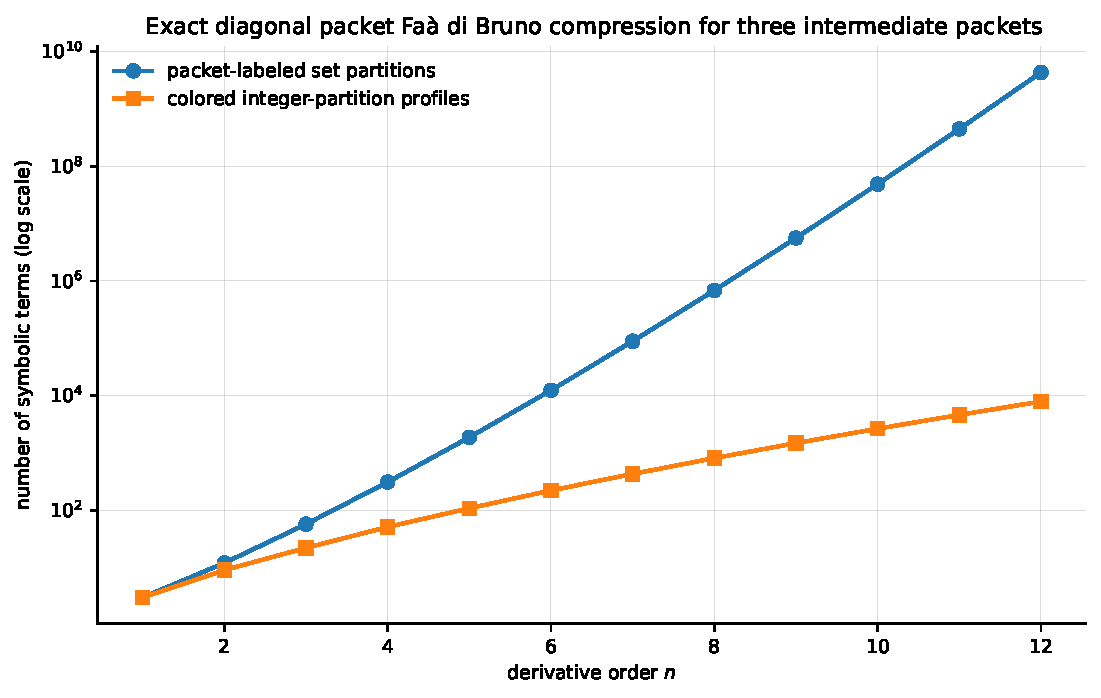
\includegraphics[width=.88\textwidth]{faa_di_bruno_compression.pdf}
\caption{For repeated directions, packet-labeled set partitions collapse to colored integer-partition profiles.  The compression is exact, not asymptotic.}
\label{fig:block11-faa-compression}
\end{figure}

\begin{boundary}[Scope of the compression theorem]
Equation \textup{(11.5)} closes the repeated-direction, single-input-packet case.  For fully mixed directions, blocks carry the types of their actual input subsets; the relevant orbit type is finer and can approach the full set-partition expansion.  No universal mixed-direction compression ratio is asserted.
\end{boundary}

\subsection{The cyclic nonlinear core of a packet system}
\label{subsec:block11-dependency-core}

For the packet system \textup{(11.4)}, define the directed dependency graph $G_\Phi$ on $I$ by placing an edge
\[
 j\longrightarrow i
\]
when some active block contributing to the equation for $u_i$ contains $u_j$ as an input.  Let
\[
 \operatorname{SCC}(G_\Phi)
\]
be its strongly connected components.  A component is called cyclic when it contains more than one address or is a singleton carrying a self-loop.

\begin{definition}[Address-preserving cyclic dimension]
The cyclic packet dimension of the marked system is
\[
 \boxed{
 \operatorname{cdim}_{\mathcal P}(\Phi)
 =
 \sum_{C\text{ cyclic SCC}}|C|.}
 \tag{11.7}
\]
It measures the number of packet variables that remain in coupled nonlinear components after exact elimination of the acyclic singleton components.
\end{definition}

\begin{theorem}[Exact SCC reduction]
\label{thm:block11-scc-reduction}
Order the SCC condensation graph topologically.  Every acyclic singleton component can be substituted exactly once its predecessors have been determined.  Repeating this elimination gives a solution-preserving bijection between:
\begin{enumerate}
\item solutions of the full packet system, and
\item solutions of the subsystem supported on the cyclic SCCs, followed by deterministic reconstruction along the condensation graph.
\end{enumerate}
Consequently, the coupled nonlinear core has exactly $\operatorname{cdim}_{\mathcal P}(\Phi)$ packet variables.
\end{theorem}

\begin{proof}
A singleton SCC without a self-loop has an equation in which its own variable does not occur.  Once all predecessor components are known, that equation computes the variable directly.  Substituting this expression into every successor equation is an algebraic identity and gives a bijection of solution sets.  The condensation graph is acyclic, so repeated topological elimination terminates.  Components containing a directed cycle cannot be removed by this one-pass address-preserving substitution because each contains a variable depending, directly or transitively, on itself.
\end{proof}

\begin{figure}[htbp]
\centering
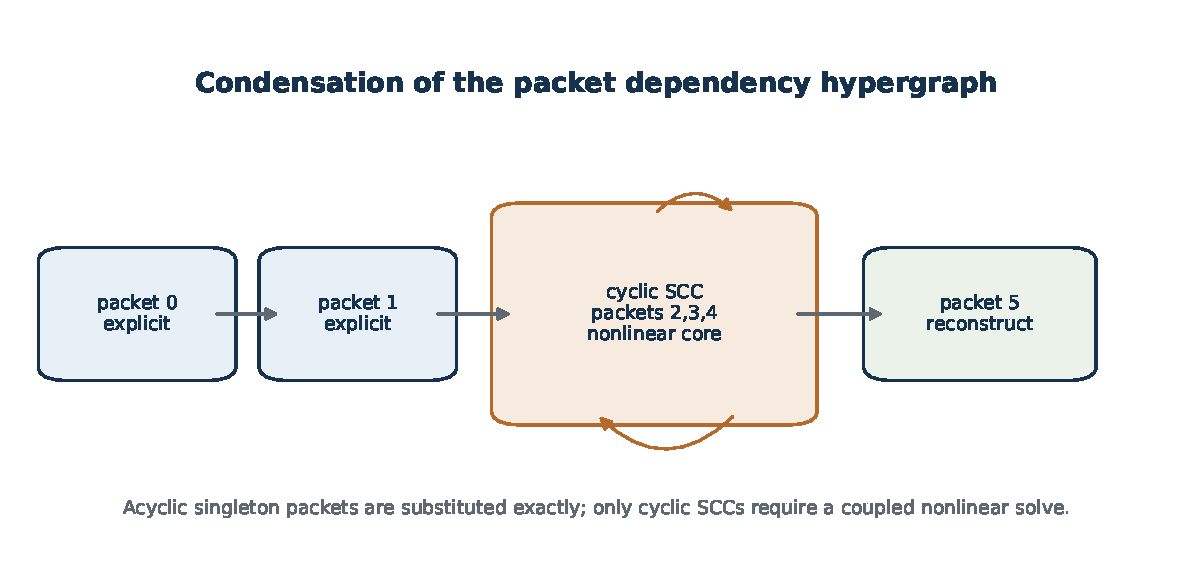
\includegraphics[width=.94\textwidth]{nonlinear_dependency_core.pdf}
\caption{Condensation separates exact one-pass reconstruction from the cyclic nonlinear core.  The resulting dimension is relative to the declared packet coordinates.}
\label{fig:block11-dependency-core}
\end{figure}

\begin{boundary}[Not a universal nonlinear state minimum]
The quantity \(\operatorname{cdim}_{\mathcal P}\) is invariant under relabeling of the declared packet system and exact elimination within its dependency grammar.  A nonlinear change of variables, hidden-variable introduction, algebraic elimination, or another packet family can change it.  It is therefore a certified address-preserving system dimension, not a universal minimum over all nonlinear presentations.
\end{boundary}

\subsection{A finite residue signature for simply generated trees}
\label{subsec:block11-tree-signature}

Consider the scalar marked equation
\[
 \boxed{
 u(z)=z+\Phi(u(z)),
 \qquad
 \Phi(y)=\sum_{m\in\mathcal A}w_my^m,}
 \tag{11.8}
\]
where $\mathcal A\subseteq\{2,3,\ldots\}$ is finite and every $w_m$ is a positive integer.  Its unique formal solution belongs to $z\mathbb Z[[z]]$ and counts plane rooted trees whose internal arities lie in $\mathcal A$, weighted by the $w_m$.

Define the arity period
\[
 \boxed{
 d_{\mathcal A}
 =
 \gcd\{m-1:m\in\mathcal A\}.}
 \tag{11.9}
\]
Every tree with internal vertices $v$ has leaf count
\[
 \ell(T)=1+\sum_{v}(\deg(v)-1).
\]

\begin{theorem}[Finite tree-address signature]
\label{thm:block11-tree-address}
Fix a packet width $N$ and put
\[
 g_N=\gcd(N,d_{\mathcal A}).
\]
For the arithmetic packets
\[
 U_j(x)=\sum_{r\ge0}[z^{Nr+j}]u(z)\,x^r,
\]
the following are equivalent:
\begin{enumerate}
\item $U_j\neq0$;
\item $j-1$ belongs to the subgroup of $\mathbb Z/N\mathbb Z$ generated by $\{m-1:m\in\mathcal A\}$;
\item
\[
 \boxed{j\equiv1\pmod{g_N}.}
\]
\end{enumerate}
Hence the exact number of active packet addresses is
\[
 \boxed{
 \#\operatorname{Supp}_N(u)=\frac{N}{g_N}.}
 \tag{11.10}
\]
\end{theorem}

\begin{proof}
Replacing one leaf by an $m$-ary vertex increases the leaf count by $m-1$.  Starting from the one-leaf tree, every nonnegative sum of allowed increments is realized by a sequence of leaf replacements.  Positivity of the weights prevents cancellation, so the coefficient support is exactly
\[
 1+\left\langle m-1:m\in\mathcal A\right\rangle_{\mathbb N}.
\]
Modulo $N$, the monoid generated by the increments equals the subgroup they generate because every element of a finite cyclic subgroup has a nonnegative representative.  That subgroup is $g_N\mathbb Z/N\mathbb Z$, which proves the congruence and the count.
\end{proof}

\begin{corollary}[Finite bottom-up residue automaton]
Label every leaf by $1\in\mathbb Z/N\mathbb Z$ and every $m$-ary vertex by the sum of its child labels.  The reachable state set is exactly
\[
 \{j:j\equiv1\pmod{g_N}\}.
\]
Thus the finite pair
\[
 \boxed{
 \mathfrak T_N(\mathcal A)
 =
 (d_{\mathcal A},g_N,N/g_N)}
 \tag{11.11}
\]
classifies packet support for the marked simply generated family.
\end{corollary}

\begin{figure}[htbp]
\centering
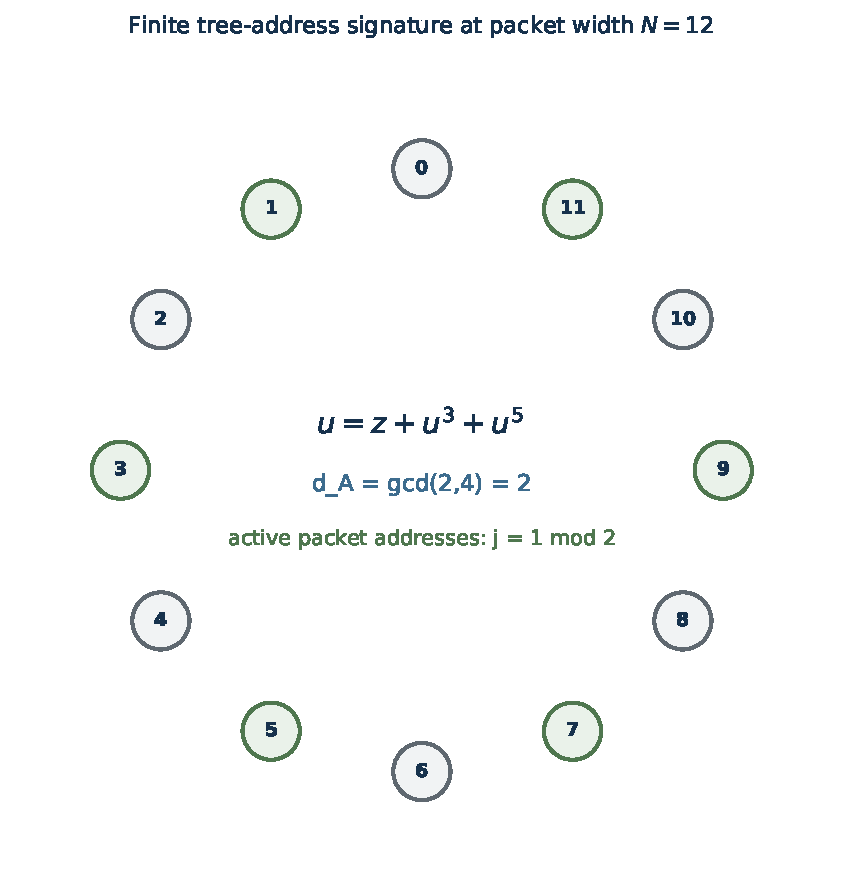
\includegraphics[width=.72\textwidth]{tree_residue_signature.pdf}
\caption{For arities three and five, the increment gcd is two.  At width twelve, exactly the six addresses congruent to one modulo two are active.}
\label{fig:block11-tree-residue}
\end{figure}

\subsection{Dominant singularity orbits}
\label{subsec:block11-tree-singularity}

Assume now that the coefficients $w_m$ are positive real numbers.  The classical smooth implicit-function schema for simply generated trees applies when there is a positive solution $\tau$ of
\[
 \Phi'(\tau)=1
\]
and
\[
 \rho=\tau-\Phi(\tau)>0.
\]
Under its standard nondegeneracy hypotheses, the reduced aperiodic series has a square-root singularity at its positive radius \cite{FlajoletSedgewick2009}.  The arity period restores the complete source orbit.

\begin{theorem}[Complete dominant-orbit signature]
\label{thm:block11-dominant-orbit}
Under the smooth implicit schema, the dominant singularities of $u(z)$ form
\[
 \boxed{
 \rho\,\mu_{d_{\mathcal A}},}
 \tag{11.12}
\]
where $\mu_d$ is the group of $d$th roots of unity.  After packetization with $x=z^N$, the union of dominant singularities of the complete packet tuple is
\[
 \boxed{
 \rho^N\,\mu_{h_N},
 \qquad
 h_N=\frac{d_{\mathcal A}}{\gcd(N,d_{\mathcal A})}.}
 \tag{11.13}
\]
Therefore the same finite arity signature determines both the number of active packet addresses and the size of the complete dominant-singularity orbit.
\end{theorem}

\begin{proof}
By \cref{thm:block11-tree-address}, the coefficient support is contained in $1+d_{\mathcal A}\mathbb N$ and the reduced exponent set is aperiodic by maximality of the gcd.  Hence
\[
 u(z)=zV(z^{d_{\mathcal A}})
\]
with $V$ aperiodic.  The smooth implicit schema gives one positive dominant singularity for $V$, and pulling back through $z^{d_{\mathcal A}}$ gives \textup{(11.12)}.  The map $z\mapsto z^N$ sends $\mu_{d_{\mathcal A}}$ onto a root group of cardinality
\[
 d_{\mathcal A}/\gcd(N,d_{\mathcal A}).
\]
No packet can introduce a new dominant image outside this set.  Conversely, if every packet were analytic at one image, the exact synthesis
\[
 u(z)=\sum_{j=0}^{N-1}z^jU_j(z^N)
\]
would make $u$ analytic at every source point above that image, contradicting \textup{(11.12)}.  Thus the union of packet singularities is exactly \textup{(11.13)}.
\end{proof}

\begin{figure}[htbp]
\centering
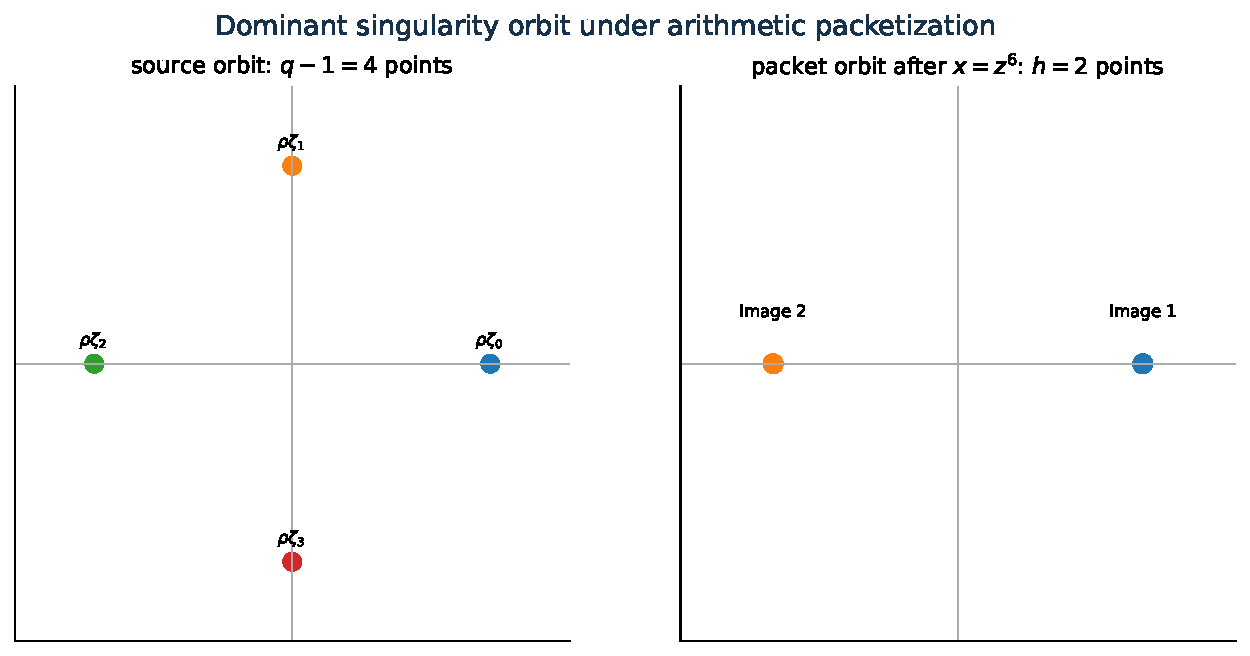
\includegraphics[width=.94\textwidth]{tree_singularity_orbit.pdf}
\caption{Arithmetic packetization maps the source root-of-unity singularity orbit through $z\mapsto z^N$.  Distinct source singularities can alias to one packet-variable singularity.}
\label{fig:block11-tree-singularity}
\end{figure}

\begin{boundary}[Individual-packet cancellation]
The theorem identifies the union of dominant singularities of the complete packet tuple.  One individual packet can lose some orbit points through address cancellation.  The finite signature does not, by itself, determine every individual local amplitude or cancellation coefficient.
\end{boundary}

\subsection{\texorpdfstring{The sharp full \(q\)-ary family}{The sharp full q-ary family}}
\label{subsec:block11-qary}

Take
\[
 \boxed{u=z+u^q,\qquad q\ge2.}
 \tag{11.14}
\]
Lagrange inversion gives the exact coefficient formula
\[
 \boxed{
 [z^n]u
 =
 \begin{cases}
 \displaystyle
 \frac{1}{(q-1)m+1}\binom{qm}{m},
 &n=1+(q-1)m,\\[9pt]
 0,&n\not\equiv1\pmod{q-1}.
 \end{cases}}
 \tag{11.15}
\]
The nonzero coefficients are the Fuss--Catalan numbers of full plane $q$-ary trees.

Write
\[
 u(z)=\sum_{j=0}^{N-1}z^jU_j(z^N),
 \qquad x=z^N.
\]

\begin{theorem}[Exact $q$-ary packet phase theorem]
\label{thm:block11-qary-phase}
Put
\[
 g=\gcd(N,q-1),
 \qquad
 h=\frac{q-1}{g}.
\]
Then:
\begin{enumerate}
\item the active packet addresses are exactly
\[
 \boxed{j\equiv1\pmod g;}
\]
\item the complete packet system is
\[
\boxed{
 U_j(x)
 =
 \delta_{j,1}
 +
 \sum_{\substack{0\le r_1,\ldots,r_q<N\\
 r_1+\cdots+r_q\equiv j\ (\mathrm{mod}\ N)}}
 x^{(r_1+\cdots+r_q-j)/N}
 \prod_{a=1}^{q}U_{r_a}(x);}
 \tag{11.16}
\]
\item the smooth critical values are
\[
 \tau=q^{-1/(q-1)},
 \qquad
 \rho=(q-1)q^{-q/(q-1)};
\]
\item the source dominant orbit has $q-1$ points, while the complete packet orbit has exactly $h$ points.
\end{enumerate}
The phase is therefore determined by the finite tuple
\[
 \boxed{(q,N,g,N/g,h).}
 \tag{11.17}
\]
\end{theorem}

\begin{proof}
Formula \textup{(11.15)} follows from Lagrange inversion applied to
\[
 z=u(1-u^{q-1}).
\]
The support and active-address statements are \cref{thm:block11-tree-address} with $d_{\mathcal A}=q-1$.  Expanding $u^q$ in complete packets and collecting the exponent carry
\[
 r_1+\cdots+r_q=j+Nc
\]
gives \textup{(11.16)}.  The critical equations
\[
 q\tau^{q-1}=1,
 \qquad
 \rho=\tau-\tau^q
\]
give the printed values, and \cref{thm:block11-dominant-orbit} gives the orbit count.
\end{proof}

\begin{table}[htbp]
\centering
\caption{Exact packet signatures for the marked full $q$-ary tree family $u=z+u^q$.}
\label{tab:block11-qary-phases}
\small
\begin{tabular}{rrrrrr}
\toprule
$q$ & $N$ & $g=\gcd(N,q-1)$ & Active packets & Packet orbit & Active addresses\\
\midrule
2 & 5 & 1 & 5 & 1 & $\{0,1,2,3,4\}$\\
3 & 4 & 2 & 2 & 1 & $\{1,3\}$\\
3 & 5 & 1 & 5 & 2 & $\{0,1,2,3,4\}$\\
4 & 4 & 1 & 4 & 3 & $\{0,1,2,3\}$\\
4 & 6 & 3 & 2 & 1 & $\{1,4\}$\\
5 & 6 & 2 & 3 & 2 & $\{1,3,5\}$\\
5 & 7 & 1 & 7 & 4 & $\{0,1,2,3,4,5,6\}$\\
6 & 10 & 5 & 2 & 1 & $\{1,6\}$\\
\bottomrule
\end{tabular}
\end{table}


\subsection{Verification, status, and exact boundary}
\label{subsec:block11-validation}

The Nonlinear tree atlas verifier performs four independent exact audits.  It enumerates colored integer-partition profiles and compares their orbit-weighted Fa\`a di Bruno values with the full set-partition expansion.  It constructs exact fixed-point prefixes for marked polynomial tree families and checks the finite arity-gcd support theorem over many packet widths.  It verifies Fuss--Catalan formulas and the complete carry-form packet equations for the full $q$-ary family.  Finally, it checks dependency-graph reductions against exhaustive bounded graph instances.

\begin{table}[htbp]
\centering
\caption{Exact finite verification for Nonlinear tree atlas.}
\label{tab:block11-validation}
\small
\begin{tabularx}{\textwidth}{@{}Y r@{}}
\toprule
Validation class & Exact checks\\
\midrule
Colored profile counts & 100\\
Orbit-size identity & 48\\
Exact compressed Faà di Bruno values & 126\\
Polynomial fixed-point prefixes & 300\\
Finite tree-address signatures & 70,458\\
Fuss-Catalan formulas & 2,892\\
Exact q-ary packet systems & 37,567\\
Dominant-orbit combinatorics & 176\\
Dependency-core reductions & 4,054\\
\midrule
\textbf{Nonlinear tree atlas total} & \textbf{115,721}\\
Cumulative the preceding certified atlas program total & 2,027,665\\
Failures & 0\\
\bottomrule
\end{tabularx}
\end{table}


\begin{resultbox}
\textbf{Section result.}
Marked polynomial fixed-point systems admit exact packet, hypergraph, operadic-tree, and packet-equation charts.  The repeated-direction packet Fa\`a di Bruno expansion compresses exactly from colored set partitions to colored integer-partition profiles.  The packet dependency graph has an exact SCC reduction whose cyclic vertices form the address-preserving nonlinear core.  For positive simply generated tree systems, the arity gcd is a finite signature determining every arithmetic packet-support pattern and the complete dominant-singularity orbit.  The full $q$-ary family supplies a closed Fuss--Catalan phase theorem and exact packet equations.
\end{resultbox}

\begin{boundarybox}
\textbf{Exact boundary of Nonlinear tree atlas.}
The atlas classifies marked polynomial systems, not semantic fixed points independently of their generators.  The compression theorem treats repeated directions; arbitrary mixed-direction jets can require a finer orbit type.  The SCC dimension is relative to the declared packet coordinates.  The tree signature classifies support and the complete dominant-singularity orbit for the marked simply generated family.  It does not classify algebraic degree, universal minimal system dimension, every individual packet amplitude, arbitrary sign-canceling weights, noncontractive global dynamics, or all nonlinear operadic systems.
\end{boundarybox}


\section{Finite Galois, profinite, and Tannakian resolved symmetry}
\label{sec:block12-galois-tannakian}

Galois-Tannakian atlas develops the final declared stratum in the present eight-stratum program: finite semisimple Galois charts, cohomological descent, profinite refinement, and the tensor-fiber boundary at which a symmetry group can be reconstructed.  The strongest Galois source already contains Reynolds projectors, the subgroup--fixed-field correspondence, normality and quotient compression, conjugate projector atlases, Mackey double-coset packets, ramification details, Haar projectors, Hilbert 90, the Brauer obstruction, finite \(\acute{e}\)tale permutation resolutions, and neutral Tannakian reconstruction \cite{GAL}.  The purpose here is to place those results into the same passport, bridge, obstruction, and effective-descent language used by the preceding sections.

The scope is deliberately semisimple or tensor-exact.  For finite group averaging, the coefficient field has characteristic zero or characteristic prime to the relevant group order.  Linear semilinear descent is taken over a finite Galois extension.  Projective descent is typed separately from vector descent.  Tannakian reconstruction is asserted only after a faithful exact tensor fiber functor has been supplied.  Modular fixed points, wild integral descent, nonneutral fiber functors, and derived or flat replacements for failed averaging remain outside this block.

\subsection{Finite subgroup, fixed-field, and Reynolds-projector charts}
\label{subsec:block12-reynolds}

Let \(L/K\) be a finite Galois extension with group
\[
 G=\operatorname{Gal}(L/K).
\]
Let \(V\) be a finite-dimensional representation of \(G\) over a characteristic-zero field, or a unitary complex realization obtained after scalar extension.  For every subgroup \(H\leq G\), define
\[
 \boxed{
 P_H=\frac1{|H|}\sum_{h\in H}U_h.}
 \tag{12.1}
\]

\begin{theorem}[Reynolds fixed packet and reverse order]
\label{thm:block12-reynolds}
The operator \(P_H\) is the projector onto the fixed packet
\[
 V^H=\{v:U_hv=v\text{ for all }h\in H\}.
\]
If \(H\leq J\), then
\[
 \boxed{P_HP_J=P_JP_H=P_J.}
 \tag{12.2}
\]
Consequently, subgroup inclusion reverses the fixed-projector order.
\end{theorem}

\begin{proof}
The average is invariant under left and right multiplication by elements of \(H\).  Therefore \(P_H^2=P_H\), and its range is exactly the fixed subspace.  If \(H\leq J\), then \(V^J\subseteq V^H\).  The two projections are nested and multiply to the projector with smaller range.
\end{proof}

In the faithful regular realization, or in the field realization supplied by a normal basis, the projector determines the subgroup.  Indeed, the support of the group-algebra idempotent
\[
 e_H=\frac1{|H|}\sum_{h\in H}h
\]
is exactly \(H\).

\begin{theorem}[Normalized finite Galois chart]
\label{thm:block12-normalized-galois-chart}
Fix the finite Galois extension \(L/K\).  The following data determine one another exactly:
\[
 \boxed{
 H
 \quad\longleftrightarrow\quad
 L^H
 \quad\longleftrightarrow\quad
 P_H
 }
 \tag{12.3}
\]
where the projector is taken in a faithful field or regular realization.  The correspondence is order reversing:
\[
 H\leq J
 \quad\Longleftrightarrow\quad
 L^H\supseteq L^J
 \quad\Longleftrightarrow\quad
 P_H\geq P_J.
\]
Thus the subgroup poset, the intermediate-field poset, and the faithful fixed-projector poset form three normalized charts of one finite semisimple Galois object.
\end{theorem}

\begin{proof}
The finite Galois correspondence gives \(H=\operatorname{Gal}(L/L^H)\) and \(E=L^{\operatorname{Gal}(L/E)}\).  The range of \(P_H\) is \(L^H\) after faithful scalar extension, and the support of \(e_H\) recovers \(H\).  All three assignments are therefore mutually inverse on the declared charts.
\end{proof}

\begin{figure}[htbp]
\centering
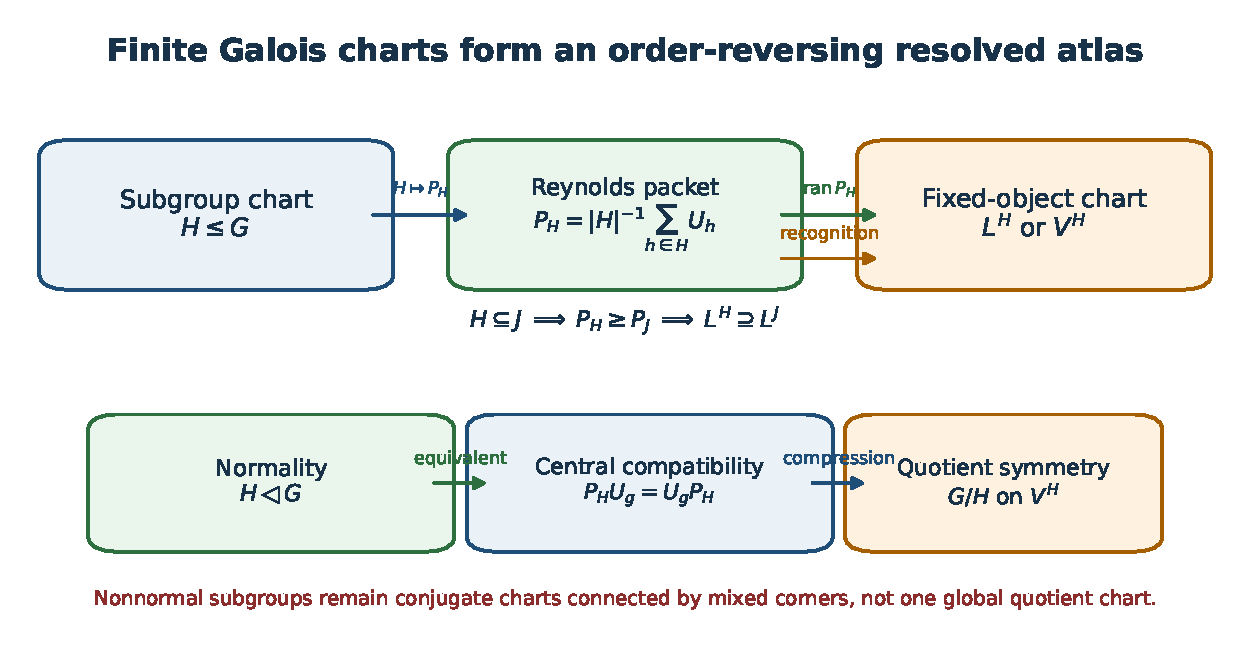
\includegraphics[width=.97\textwidth]{galois_subgroup_atlas.pdf}
\caption{The finite subgroup, Reynolds-projector, and fixed-field charts are reversible in a faithful semisimple realization.  Normality is the additional condition required for quotient compression.}
\label{fig:block12-subgroup-atlas}
\end{figure}

\subsection{Compatibility, normality, and conjugate atlases}
\label{subsec:block12-normality}

For two subgroups \(H,J\leq G\), the common fixed packet is always
\[
 V^H\cap V^J=V^{\langle H,J\rangle}.
\]
The two averaging projectors need not commute.

\begin{theorem}[Permutable subgroups and exact common refinement]
\label{thm:block12-permutable}
In a faithful regular realization, the following are equivalent:
\begin{enumerate}
\item \(HJ=JH\);
\item \(HJ\) is a subgroup of \(G\);
\item \(P_HP_J=P_JP_H\).
\end{enumerate}
When these conditions hold,
\[
 \boxed{P_HP_J=P_{HJ}.}
 \tag{12.4}
\]
If they fail, \(P_HP_J\) and \(P_JP_H\) are mixed atlas corners rather than projectors.
\end{theorem}

\begin{proof}
If \(HJ=JH\), every element of \(HJ\) has \(|H\cap J|\) representations as \(hj\).  Multiplying the two group averages therefore gives the average over \(HJ\).  Conversely, the support of \(e_He_J\) is \(HJ\), while the support of \(e_Je_H\) is \(JH\).  Equality in the regular group algebra forces equality of the product sets.
\end{proof}

\begin{theorem}[Normality and quotient compression]
\label{thm:block12-normality}
For a subgroup \(H\leq G\), the following conditions are equivalent:
\begin{enumerate}
\item \(H\triangleleft G\);
\item \(e_H\) is central in the group algebra;
\item \(P_HU_g=U_gP_H\) for every \(g\in G\);
\item the fixed packet \(V^H\) is \(G\)-invariant;
\item the fixed field \(L^H\) is Galois over \(K\).
\end{enumerate}
When they hold, the compressed action on \(V^H\) factors through \(G/H\), and
\[
 \boxed{\operatorname{Gal}(L^H/K)\cong G/H.}
 \tag{12.5}
\]
\end{theorem}

\begin{proof}
Conjugation sends \(e_H\) to \(e_{gHg^{-1}}\).  Centrality is therefore equivalent to normality.  The represented identity
\[
 U_gP_HU_g^{-1}=P_{gHg^{-1}}
\]
gives the operator conditions.  The field and quotient statements are the normal-subgroup part of the finite Galois correspondence.
\end{proof}

If \(H\) is not normal, its conjugates form a genuine atlas rather than one quotient chart.  Put
\[
 \operatorname{Core}_G(H)=\bigcap_{g\in G}gHg^{-1},
 \qquad
 \operatorname{Ncl}_G(H)=\left\langle gHg^{-1}:g\in G\right\rangle.
\]

\begin{theorem}[Canonical envelopes of a nonnormal Galois atlas]
\label{thm:block12-core-normal-closure}
Let \(M=L^H\).  Then
\[
 \boxed{
 L^{\operatorname{Core}_G(H)}
 =\prod_{g\in G}g(M)}
 \tag{12.6}
\]
is the smallest Galois extension inside \(L\) containing every conjugate chart, while
\[
 \boxed{
 L^{\operatorname{Ncl}_G(H)}
 =\bigcap_{g\in G}g(M)}
 \tag{12.7}
\]
is the largest Galois subfield contained in every chart.  The core and normal-closure projectors are the two canonical global envelopes of the conjugate atlas.
\end{theorem}

\begin{proof}
Composita of intermediate fields correspond to intersections of subgroups, while intersections of fields correspond to generated subgroups.  The core is the largest normal subgroup inside \(H\), and the normal closure is the smallest normal subgroup containing \(H\).
\end{proof}

\begin{example}[The \(S_3\) nonnormal atlas]
Let \(G=S_3\) and let \(H\) be generated by one transposition.  There are three conjugate order-two subgroups and hence three conjugate cubic fixed-field charts.  Their subgroup core is trivial, while their normal closure is all of \(S_3\).  By contrast, the order-three subgroup \(A_3\) is normal and its fixed chart carries the quotient symmetry \(S_3/A_3\cong C_2\).
\end{example}

\subsection{Double cosets as exact transition packets}
\label{subsec:block12-mackey}

Restriction and induction connect subgroup charts that need not commute.  Their exact address set is the double-coset space
\[
 K\backslash G/H.
\]

\begin{theorem}[Mackey transition-packet decomposition]
\label{thm:block12-mackey}
Let \(H,K\leq G\), let \(W\) be a finite-dimensional representation of \(H\), and choose representatives \(x\) for \(K\backslash G/H\).  Then
\[
 \boxed{
 \operatorname{Res}_K^G\operatorname{Ind}_H^GW
 \cong
 \bigoplus_{x\in K\backslash G/H}
 \operatorname{Ind}_{K\cap xHx^{-1}}^K
 \left({}^x\operatorname{Res}_{H\cap x^{-1}Kx}^HW\right).}
 \tag{12.8}
\]
Each double coset is one exact transfer packet between the \(H\)- and \(K\)-charts.
\end{theorem}

\begin{proof}
The induced representation is a function space on \(G\) with \(H\)-covariance.  Functions supported on different double cosets are invariant direct summands under \(K\).  Identifying the summand on \(KxH\) with an induced representation from \(K\cap xHx^{-1}\) gives the decomposition.
\end{proof}

The dimension identity for the trivial \(H\)-representation is
\[
 \boxed{
 [G:H]
 =
 \sum_{x\in K\backslash G/H}
 [K:K\cap xHx^{-1}].}
 \tag{12.9}
\]
This is the finite packet-count law audited by the Galois-Tannakian atlas verifier.

\begin{figure}[htbp]
\centering
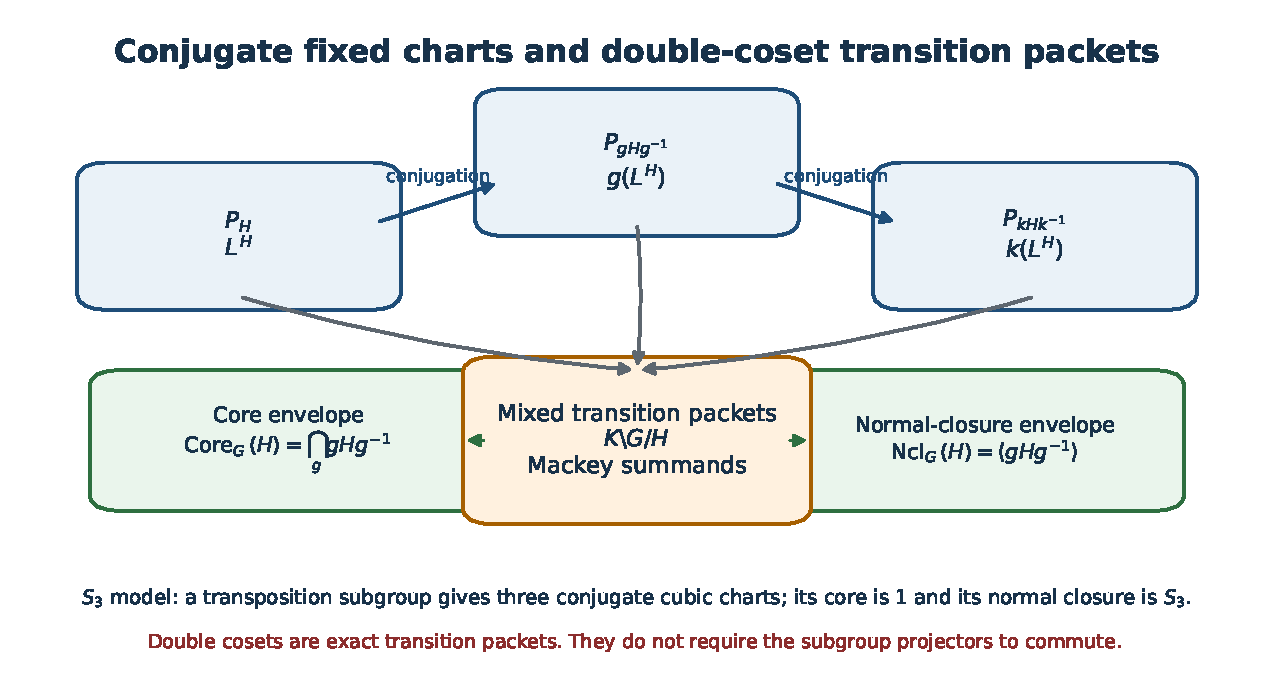
\includegraphics[width=.97\textwidth]{galois_mackey_packets.pdf}
\caption{A nonnormal fixed object is an atlas of conjugate charts.  Core and normal closure give two global envelopes, while double cosets give exact mixed transition packets.}
\label{fig:block12-mackey}
\end{figure}

\begin{table}[htbp]
\centering
\caption{Finite group models used in the Galois-Tannakian atlas subgroup-projector audit.}
\label{tab:block12-groups}
\scriptsize
\begin{tabularx}{\textwidth}{@{}L{0.12\textwidth}rrrrrY@{}}
\toprule
Group & Order & Subgroups & Normal & Permutable ordered pairs & Noncommuting ordered pairs & Double-coset packets audited\\
\midrule
C2 & 2 & 2 & 2 & 4 & 0 & 5\\
C3 & 3 & 2 & 2 & 4 & 0 & 6\\
C4 & 4 & 3 & 3 & 9 & 0 & 15\\
C5 & 5 & 2 & 2 & 4 & 0 & 8\\
C6 & 6 & 4 & 4 & 16 & 0 & 30\\
C8 & 8 & 4 & 4 & 16 & 0 & 37\\
V4 & 4 & 5 & 5 & 25 & 0 & 37\\
S3 & 6 & 6 & 3 & 30 & 6 & 65\\
D4 & 8 & 10 & 6 & 92 & 8 & 195\\
A4 & 12 & 10 & 3 & 64 & 36 & 250\\
\bottomrule
\end{tabularx}
\end{table}


\subsection{Ramification as a nested resolution}
\label{subsec:block12-ramification}

Let \(L/K\) be a finite Galois extension of local fields.  Write
\[
 G_0\supseteq G_1\supseteq G_2\supseteq\cdots
\]
for the lower ramification filtration after inertia, and let \(V\) be a finite-dimensional complex representation of \(G\).  Define
\[
 P_i=\frac1{|G_i|}\sum_{g\in G_i}U_g.
\]
The ramification groups are nested and normal, so
\[
 P_0\leq P_1\leq P_2\leq\cdots\leq I.
\]
Put
\[
 D_i=P_{i+1}-P_i.
\]

\begin{theorem}[Orthogonal ramification details]
\label{thm:block12-ramification-details}
The operators \(D_i\) are mutually orthogonal projectors, and
\[
 \boxed{
 V=V^{G_0}\oplus\bigoplus_i D_iV.}
 \tag{12.10}
\]
Every detail packet is stable under the quotient action permitted by the corresponding normal subgroup.
\end{theorem}

\begin{proof}
Nested orthogonal projectors commute, and the difference of two nested projectors is a projector onto the orthogonal difference of their ranges.  The decomposition follows by telescoping.
\end{proof}

\begin{theorem}[Artin conductor as weighted unresolved rank]
\label{thm:block12-artin-conductor}
The Artin and Swan conductors satisfy
\[
 \boxed{
 a(V)=\sum_{i\geq0}\frac{|G_i|}{|G_0|}\operatorname{Tr}(I-P_i),}
 \tag{12.11}
\]
\[
 \boxed{
 \operatorname{Sw}(V)=\sum_{i\geq1}\frac{|G_i|}{|G_0|}\operatorname{Tr}(I-P_i).}
 \tag{12.12}
\]
If \(d_j=\operatorname{rank}D_j\), then
\[
 \boxed{
 a(V)=\sum_jd_j\sum_{i=0}^{j}\frac{|G_i|}{|G_0|}.}
 \tag{12.13}
\]
Thus the conductor is the weighted total rank that remains unresolved at each ramification scale.
\end{theorem}

\begin{proof}
The classical conductor formula uses \(\operatorname{codim}V^{G_i}\).  Since \(P_i\) projects onto \(V^{G_i}\), this codimension is \(\operatorname{Tr}(I-P_i)\).  Also
\[
 \operatorname{codim}V^{G_i}=\sum_{j\geq i}d_j.
\]
Reversing the finite sums gives the detail formula.
\end{proof}

\begin{figure}[htbp]
\centering
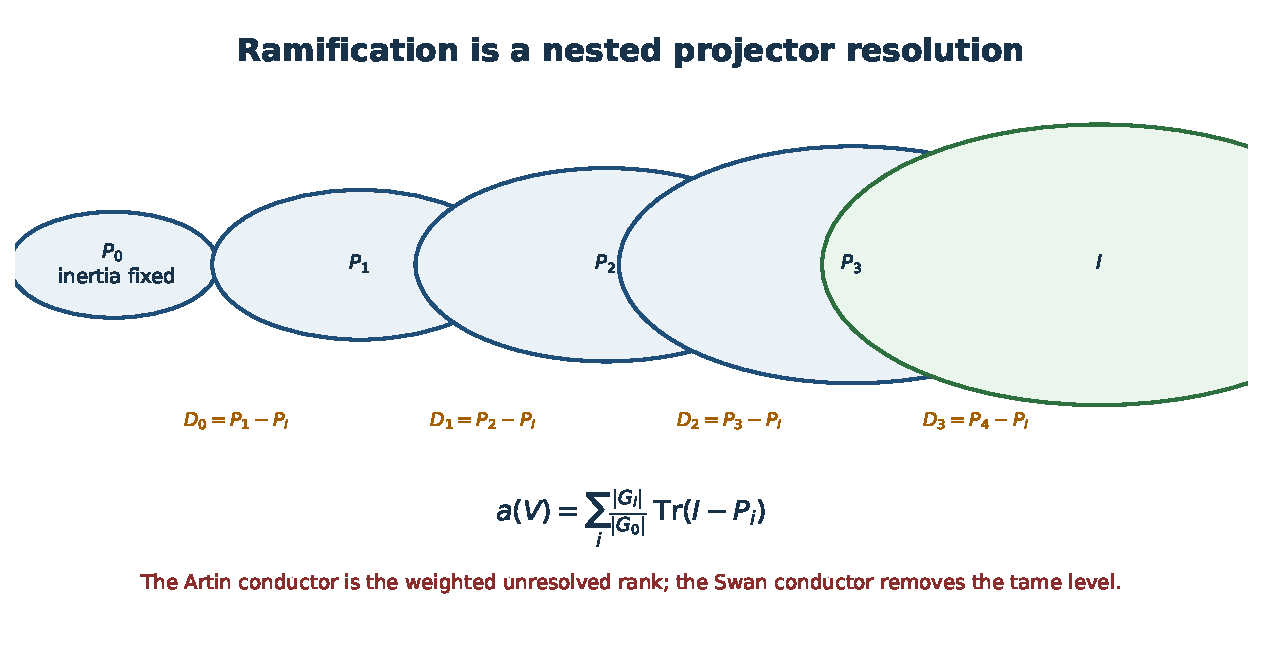
\includegraphics[width=.92\textwidth]{galois_ramification_resolution.pdf}
\caption{Ramification subgroups give nested fixed projectors.  Their orthogonal differences are the resolved tame and wild detail packets, and the conductor is their weighted unresolved rank.}
\label{fig:block12-ramification}
\end{figure}

\subsection{Profinite completion and finite quotient effectivity}
\label{subsec:block12-profinite}

Let \(G\) be a compact group and let \(U:G\to\mathcal U(\mathcal H)\) be strongly continuous.  For a closed subgroup \(H\), normalized Haar measure defines
\[
 \boxed{
 P_H=\int_HU_h\,d\mu_H(h).}
 \tag{12.14}
\]
The same averaging proof as in the finite case shows that \(P_H\) is the orthogonal projector onto \(\mathcal H^H\).

\begin{theorem}[Shrinking-subgroup reconstruction]
\label{thm:block12-shrinking-subgroups}
Let \(G\) be profinite and let
\[
 U_1\supseteq U_2\supseteq\cdots
\]
be a neighborhood basis of the identity consisting of open normal subgroups.  Then
\[
 \boxed{P_{U_n}\longrightarrow I}
 \tag{12.15}
\]
strongly in every strongly continuous unitary representation.  More generally, if \(N\triangleleft G\) is closed and \(U_n/N\) shrinks to the identity in \(G/N\), then \(P_{U_n}\to P_N\) strongly.
\end{theorem}

\begin{proof}
For each \(v\in\mathcal H\), strong continuity gives
\[
 \sup_{u\in U_n}\|U_uv-v\|\longrightarrow0.
\]
Averaging this estimate over \(U_n\) proves the first statement.  Apply it to the quotient action on the \(N\)-fixed packet for the second.
\end{proof}

\begin{corollary}[Finite-dimensional representations occur at finite level]
\label{cor:block12-finite-level}
Every continuous finite-dimensional complex representation of a profinite group has finite image and factors through a finite quotient.
\end{corollary}

\begin{proof}
The image is a compact totally disconnected subgroup of \(\operatorname{GL}_n(\mathbb C)\).  After conjugation it lies in a compact Lie group.  A compact totally disconnected Lie group is finite.
\end{proof}

This finite-level factorization is a strong effectivity statement for finite-dimensional complex representations.  It is not a statement that every integral, modular, or derived representation becomes semisimple at finite level.

\subsection{Semilinear vector descent and Hilbert 90}
\label{subsec:block12-hilbert90}

Let \(L/K\) be finite Galois with group \(G\).  A semilinear \(G\)-object is an \(L\)-vector space \(V\) with maps
\[
 \rho_\sigma:V\to V,
 \qquad
 \rho_\sigma(\lambda v)=\sigma(\lambda)\rho_\sigma(v),
\]
satisfying the group law.  Scalar extension and fixed vectors define functors
\[
 L\otimes_K-:\operatorname{Vect}_K\longrightarrow\operatorname{Semilin}_G(L),
\]
\[
 (-)^G:\operatorname{Semilin}_G(L)\longrightarrow\operatorname{Vect}_K.
\]

\begin{theorem}[Effective finite Galois vector descent]
\label{thm:block12-vector-descent}
The two functors above are quasi-inverse equivalences:
\[
 \boxed{
 \operatorname{Vect}_K
 \simeq
 \operatorname{Semilin}_G(L).}
 \tag{12.16}
\]
For every semilinear object \(V\), the fixed packet \(W=V^G\) satisfies
\[
 \boxed{W\otimes_KL\cong V.}
 \tag{12.17}
\]
The equivalence is effective on both objects and morphisms.
\end{theorem}

\begin{proof}
This is finite Galois descent.  After an \(L\)-basis is chosen, the semilinear action is represented by a cocycle
\[
 a_{\sigma\tau}=a_\sigma\sigma(a_\tau),
 \qquad
 a_\sigma\in\operatorname{GL}_n(L).
\]
Nonabelian Hilbert 90 gives \(B\in\operatorname{GL}_n(L)\) with
\[
 a_\sigma=B^{-1}\sigma(B).
\]
The columns of \(B^{-1}\) applied to a \(K\)-basis are fixed by the twisted action.  They form an \(n\)-dimensional fixed packet, and scalar extension reconstructs \(V\).  An equivariant \(L\)-linear map restricts to a \(K\)-linear map on fixed packets, and scalar extension recovers it.
\end{proof}

A useful constructive form is obtained by choosing any matrix \(C\in M_n(L)\) and setting
\[
 T(C)=\sum_{\sigma\in G}a_\sigma\sigma(C).
\]
Then
\[
 a_\tau\tau(T(C))=T(C).
\]
Whenever \(T(C)\) is invertible,
\[
 B=T(C)^{-1}
\]
is a Hilbert 90 trivialization.  Standard descent guarantees that such a \(C\) exists.

\begin{definition}[Framed semilinear descent chart]
A framed descent chart retains an ordered \(K\)-basis of the fixed packet \(W\).  Its scalar extension gives a distinguished \(L\)-basis of \(V\), and hence a literal cocycle matrix family.
\end{definition}

\begin{proposition}[Gauge and intrinsic automorphisms remain distinct]
\label{prop:block12-framed-unframed}
For fixed rank \(n\), nonabelian Hilbert 90 implies that every \(\operatorname{GL}_n(L)\)-cocycle is gauge equivalent to the trivial cocycle.  The unframed descent groupoid is not contractible: its automorphism group is \(\operatorname{GL}_n(K)\).  After a global \(K\)-frame is retained, the normalized fiber becomes contractible.
\end{proposition}

\begin{proof}
Hilbert 90 gives one isomorphism class.  Automorphisms of the descended \(K\)-space are exactly \(\operatorname{GL}_n(K)\).  A chosen ordered basis kills those automorphisms.
\end{proof}

\subsection{Projective descent and the Brauer obstruction}
\label{subsec:block12-brauer}

A projective cocycle takes values in \(\operatorname{PGL}_n(L)\).  Choose lifts
\[
 A_\sigma\in\operatorname{GL}_n(L).
\]
Their cocycle failure is scalar:
\[
 \boxed{
 c(\sigma,\tau)
 =A_\sigma\sigma(A_\tau)A_{\sigma\tau}^{-1}
 \in L^\times.}
 \tag{12.18}
\]
Changing the lifts alters \(c\) by a scalar coboundary.

\begin{theorem}[Exact projective descent obstruction]
\label{thm:block12-brauer}
The scalar class
\[
 \boxed{
 [c]=\delta([\alpha])
 \in H^2(G,L^\times)
 =\operatorname{Br}(L/K)}
 \tag{12.19}
\]
is independent of the chosen lifts.  It vanishes exactly when the projective cocycle lifts to a linear semilinear cocycle.  In that case \cref{thm:block12-vector-descent} produces a descended vector space.  If it does not vanish, the descended object is a module over a central simple \(K\)-algebra split by \(L\), not an ordinary global vector packet.
\end{theorem}

\begin{proof}
Apply the connecting map in nonabelian cohomology to
\[
 1\longrightarrow L^\times
 \longrightarrow\operatorname{GL}_n(L)
 \longrightarrow\operatorname{PGL}_n(L)
 \longrightarrow1.
\]
Vanishing is equivalent to rescaling the lifts so that the scalar defect is removed.  The lifted cocycle then descends by Hilbert 90.  The nonzero classes are the relative Brauer classes of central simple algebras split by \(L\).
\end{proof}

\begin{example}[The quaternionic obstruction over \(\mathbb C/\mathbb R\)]
Let \(G=\{1,\sigma\}\), where \(\sigma\) is complex conjugation, and put
\[
 A_\sigma=
 \begin{pmatrix}
 0&1\\
 -1&0
 \end{pmatrix}.
\]
Then
\[
 A_\sigma\sigma(A_\sigma)=-I.
\]
The projective cocycle condition holds because \(-I\) is scalar.  Its boundary is represented by \(-1\) in
\[
 \mathbb R^\times/N_{\mathbb C/\mathbb R}(\mathbb C^\times).
\]
Every complex norm is positive, so \(-1\) is nontrivial.  The descended central simple algebra is the Hamilton quaternion algebra.  Replacing \(A_\sigma\) by
\[
 \begin{pmatrix}0&1\\1&0\end{pmatrix}
\]
gives scalar defect \(+1\) and hence split vector descent.
\end{example}

\begin{figure}[htbp]
\centering
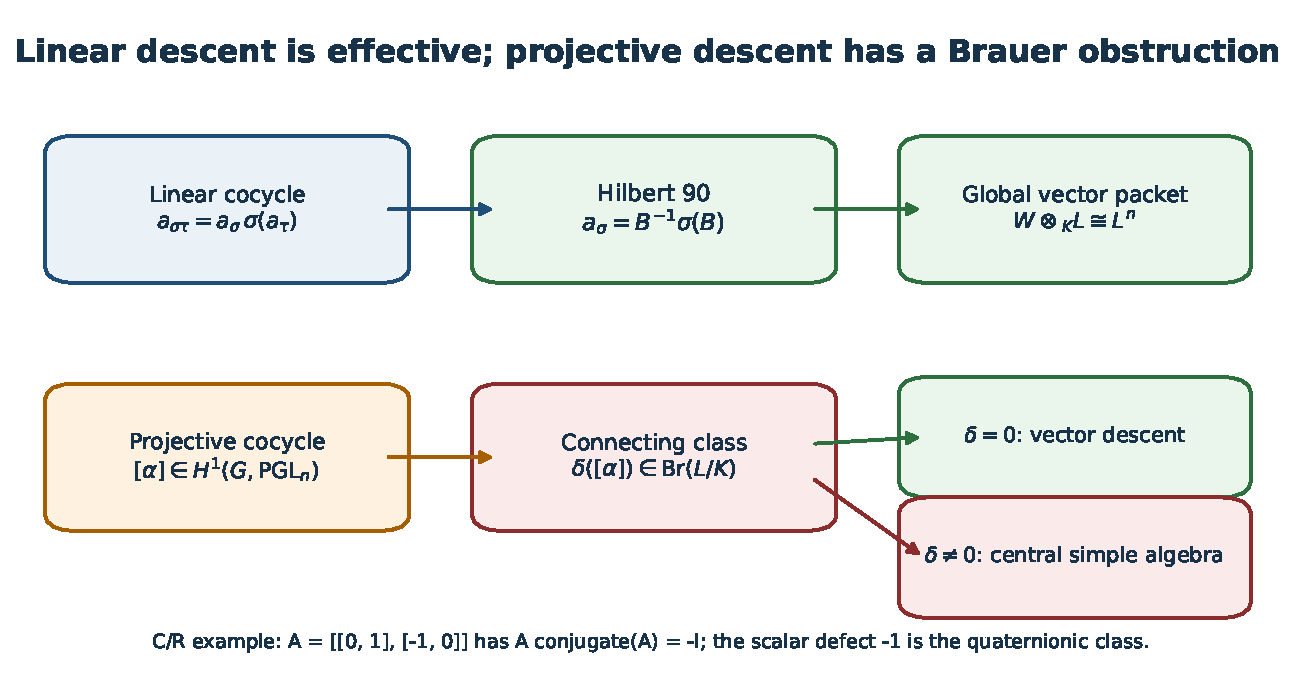
\includegraphics[width=.97\textwidth]{galois_descent_obstruction.pdf}
\caption{Linear cocycles are removed by Hilbert 90.  Projective cocycles can satisfy every visible \(\operatorname{PGL}\) overlap law while retaining a nonzero degree-two Brauer obstruction.}
\label{fig:block12-descent-obstruction}
\end{figure}

\subsection{Finite \texorpdfstring{\(\acute{e}\)}{e}tale and neutral Tannakian symmetry}
\label{subsec:block12-tannakian}

For a connected scheme \(X\) with geometric point \(\bar x\), the fiber functor on finite \(\acute{e}\)tale covers identifies that category with finite continuous \(\pi_1^{\acute{e}t}(X,\bar x)\)-sets.  Every finite fiber \(S\) produces a permutation resolution on \(\ell^2(S)\): coordinate projectors are indexed by points, orbit projectors by transitive components, and covering morphisms give equivariant packet transfers.  The profinite fundamental group is the automorphism group of this fiber functor.

The tensor-linear version requires more structure.

\begin{theorem}[Neutral Tannakian reconstruction]
\label{thm:block12-tannakian}
Let \(\mathcal C\) be a neutral Tannakian category over \(k\), and let
\[
 \omega:\mathcal C\longrightarrow\operatorname{Vect}_k
\]
be a faithful exact tensor fiber functor.  Then
\[
 \boxed{
 \mathcal G=\operatorname{Aut}^{\otimes}(\omega)}
 \tag{12.20}
\]
is an affine group scheme, and
\[
 \boxed{
 \mathcal C\simeq\operatorname{Rep}_k(\mathcal G)}
 \tag{12.21}
\]
as tensor categories.  Declared packet idempotents and refinement maps preserved by \(\omega\) become tensor-compatible concrete projector resolutions in every fiber.
\end{theorem}

\begin{proof}
The group scheme and tensor equivalence are the neutral Tannakian reconstruction theorem.  Additivity and exact tensor preservation transport the declared idempotent and refinement equations to the fibers.
\end{proof}

\begin{boundary}[Faithful corner realization is not a fiber functor]
A faithful additive or Hilbert-space realization can preserve packet idempotents, transfer blocks, and operator equations without preserving tensor products, duals, exact sequences, or the tensor unit.  Such a realization does not by itself determine \(\operatorname{Aut}^{\otimes}(\omega)\).  Tannakian symmetry begins only after the faithful exact tensor gate has been verified.
\end{boundary}

\begin{proposition}[Finite group model of the tensor boundary]
\label{prop:block12-finite-tensor-model}
Let \(G\) be finite and let \(\omega:\operatorname{Rep}_k(G)\to\operatorname{Vect}_k\) be the forgetful functor.  The regular representation is faithful, the action on tensor products is diagonal, the unit is fixed, and the dual action is inverse transpose.  These data distinguish every \(g\in G\) and realize the finite constant-group case of \cref{thm:block12-tannakian}.
\end{proposition}

\begin{proof}
Left translation on the regular representation is faithful.  Functoriality of the tensor product, unit, and dual actions is immediate from the representation axioms.  Since different group elements act differently on the regular basis, the induced tensor automorphisms are distinct.
\end{proof}

\begin{figure}[htbp]
\centering
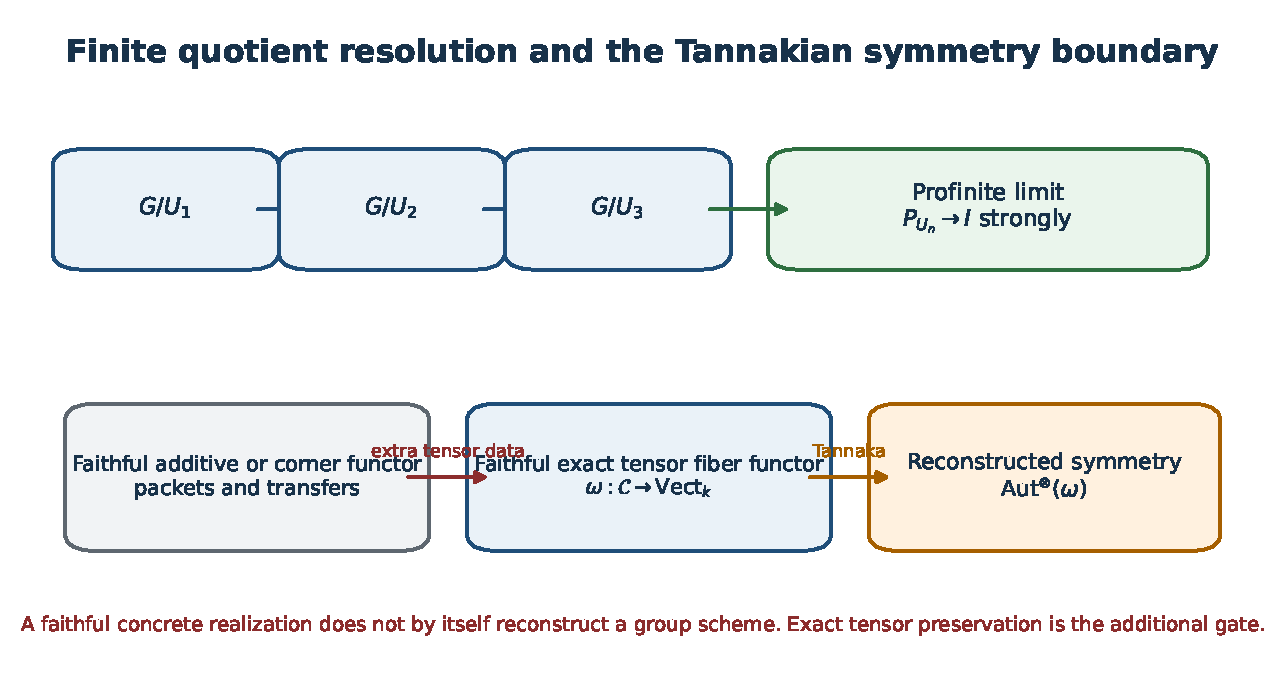
\includegraphics[width=.97\textwidth]{galois_profinite_tannakian.pdf}
\caption{Finite quotient projectors converge strongly in profinite realizations.  The lower row isolates the additional exact tensor structure required before a symmetry group scheme can be reconstructed.}
\label{fig:block12-profinite-tannakian}
\end{figure}

\subsection{The assembled finite Galois resolved atlas}
\label{subsec:block12-assembled}

The preceding results can be collected into one typed finite atlas.  The reversible charts are:
\begin{enumerate}
\item subgroups \(H\leq G\), fixed fields \(L^H\), and faithful Reynolds projectors \(P_H\);
\item finite-dimensional \(K\)-vector spaces and semilinear \(L\)-spaces with effective descent data;
\item finite \(\acute{e}\)tale fibers and their continuous permutation actions;
\item neutral Tannakian categories equipped with a specified faithful exact tensor fiber functor.
\end{enumerate}
Directional or obstructed bridges include:
\begin{enumerate}
\item restriction and induction between subgroup charts, decomposed by Mackey packets;
\item passage from a nonnormal chart to its core or normal-closure envelope;
\item projectivization from linear to projective cocycles;
\item forgetting tensor structure from a Tannakian fiber functor to an additive or corner realization;
\item passage from finite quotients to a profinite inverse system.
\end{enumerate}

\begin{theorem}[Finite semisimple Galois and Tannakian assembly]
\label{thm:block12-galois-assembly}
Under the hypotheses printed in this section:
\begin{enumerate}
\item the subgroup, fixed-field, and faithful fixed-projector charts form an order-reversing normalized atlas;
\item normal charts admit quotient compression, while nonnormal charts form conjugate projector atlases with canonical core and normal-closure envelopes;
\item double cosets give exact transition packets for induction and restriction;
\item ramification filtrations give nested fixed projectors whose weighted unresolved ranks are the Artin and Swan conductors;
\item continuous finite-dimensional profinite representations are detected at a finite quotient level;
\item linear semilinear descent is effective on objects and morphisms;
\item projective descent is effective exactly when its relative Brauer class vanishes;
\item neutral Tannakian symmetry is reconstructed exactly when a faithful exact tensor fiber functor is supplied.
\end{enumerate}
These statements form a complete assembly theorem for the declared finite semisimple and neutral tensor strata.  They do not imply effective descent for modular, wild, nonneutral, or arbitrary heterogeneous atlases.
\end{theorem}

\begin{proof}
Items 1--5 are \cref{thm:block12-normalized-galois-chart,thm:block12-normality,thm:block12-core-normal-closure,thm:block12-mackey,thm:block12-artin-conductor,cor:block12-finite-level}.  Item 6 is \cref{thm:block12-vector-descent}.  Item 7 is \cref{thm:block12-brauer}.  Item 8 is \cref{thm:block12-tannakian}.  The final boundary follows because the hypotheses used by Reynolds averaging, Hilbert 90, and neutral Tannakian reconstruction are not automatic in the excluded settings.
\end{proof}

A complete chart record on the finite subgroup locus is
\[
 \mathcal J_{L/K}(H)
 =
 \left(
 H,
 L^H,
 P_H,
 \operatorname{Core}_G(H),
 \operatorname{Ncl}_G(H),
 \{K\backslash G/H\}_{K\leq G}
 \right).
\]
The first three entries already classify the normalized object, while the remaining entries record its atlas position and transition structure.  For a framed semilinear vector object, the descended \(K\)-space with its frame is complete.  For a projective object, the Brauer class is an obstruction coordinate, not a complete invariant of all central simple algebras without the remaining algebra data.

\subsection{Exact finite verification}
\label{subsec:block12-verification}

The Galois-Tannakian atlas verifier uses exact rational group-algebra arithmetic, exact finite permutation combinatorics, and exact Gaussian-rational matrix algebra.  It audits cyclic groups, \(V_4\), \(S_3\), \(D_4\), and \(A_4\); every subgroup Reynolds idempotent; subgroup inclusion and projector order; normality and centrality; core and normal closure; commuting and noncommuting subgroup pairs; double-coset partitions and the Mackey dimension law; cyclic ramification-style filtrations; explicit Hilbert 90 coboundaries over \(\mathbb C/\mathbb R\); the split and quaternionic projective examples; and faithful regular tensor actions.

\begin{table}[htbp]
\centering
\caption{Exact verification of the Galois-Tannakian atlas finite Galois and Tannakian models.}
\label{tab:block12-validation}
\small
\begin{tabularx}{\textwidth}{@{}Y r@{}}
\toprule
Validation class & Checks\\
\midrule
Finite subgroup and Reynolds-projector identities & 1,020\\
Normality, core, and normal-closure identities & 192\\
Double-coset and Mackey packet identities & 1,590\\
Nested ramification-style projector filtrations & 39\\
Exact Hilbert 90 cocycles over Gaussian rationals & 884\\
Projective and Brauer obstruction examples & 44\\
Finite faithful tensor-model checks & 7,426\\
\midrule
\textbf{Galois-Tannakian atlas exact checks} & \textbf{11,195}\\
\textbf{Failures} & \textbf{0}\\
\bottomrule
\end{tabularx}
\end{table}


The verifier records \(11{,}195\) exact checks and no failures.  Together with the preceding certified atlas program, the cumulative exact record is
\[
 \boxed{2{,}038{,}860}
\]
checks with no recorded failures.

\begin{boundarybox}
\textbf{Exact boundary of Galois-Tannakian atlas.}
The finite subgroup/projector identities, semilinear vector descent, relative Brauer obstruction, profinite finite-level resolution, and neutral Tannakian tensor gate are established under their printed hypotheses.  The block does not prove exactness of fixed points when the group order is not invertible, derived replacement of failed Reynolds projectors, integral wild descent, classification of all central simple algebras from the Brauer class alone, existence of a neutral fiber functor, or effective descent for the entire heterogeneous Komorebi atlas.
\end{boundarybox}

\begin{resultbox}
\textbf{Section result.}
Finite semisimple Galois theory now appears as a fully typed resolved stratum.  Subgroups, fixed fields, and faithful fixed projectors are reversible charts.  Nonnormality produces conjugate atlases and mixed Mackey transition packets.  Ramification is a nested detail resolution.  Hilbert 90 makes linear semilinear descent effective, while the relative Brauer class is the exact obstruction to projective vector descent.  Profinite quotient charts reconstruct continuous finite-dimensional symmetry, and a faithful exact tensor fiber functor crosses the separate Tannakian boundary to reconstruct an affine group scheme.  This closes the declared finite Galois and neutral tensor stratum, not modular, wild, nonneutral, or unrestricted global descent.
\end{resultbox}


\part{Certified global synthesis and scope}

\section{Global invariant descent on the certified finite atlas}
\label{sec:block13-global-invariant}

Global synthesis atlas performs the assembly step requested after the native stratum invariants.  The preceding sections do not justify one unrestricted equivalence among all eight broad strata.  They do, however, supply several finite connected systems of normalized charts for which the semantic object, overlap categories, bridge directions, information loss, coherence, and local completeness are explicit.  This section freezes those systems into one authoritative certified atlas, constructs the invariant comparison maps, verifies their higher coherence, and proves the strongest global completeness theorem supported by the assembled results.

The global object in this section is deliberately a finite disjoint union of connected semantic components.  Each component contains nontrivial reversible bridges across different kinds of presentation.  The component tag is retained as part of the invariant.  No bridge is invented between two components merely because their formulas use similar words or symbols.  In particular, the functional-Mahler coefficient component and the continuous Newton--Mahler interpolation component remain distinct even though both belong to the broad local stratum.

\subsection{The authoritative bridge matrix}
\label{subsec:block13-bridge-matrix}

Write
\[
 \mathsf E,
 \quad
 \mathsf{FF},
 \quad
 \mathsf D,
 \quad
 \mathsf P,
 \quad
 \varnothing
\]
for an equivalence on a named normalized overlap, a fully faithful inclusion, an information-losing directional functor, a partial or hypothesis-dependent bridge, and the absence of a certified broad bridge, respectively.  The matrix below records only relations already established in the preceding sections or in the audited source concordance.  A symbol carrying a subscript refers to the named overlap rather than to the whole broad stratum.

\begin{landscape}
\begin{table}[p]
\centering
\caption{Authoritative broad-stratum bridge matrix for the certified global synthesis atlas. Every decorated equivalence is restricted to the named normalized overlap; the undecorated broad categories are not thereby identified.}
\label{tab:block13-bridge-matrix}
\scriptsize
\setlength{\tabcolsep}{3.7pt}
\begin{tabular}{@{}lcccccccc@{}}
\toprule
Source $\backslash$ target & LIN & HOL & DIG & ALG & TREE & PROD & LOC & GAL\\
\midrule
LIN  & $\mathsf E$ & $\mathsf{FF}$ & $\mathsf E_{\rm per}$ & -- & -- & -- & $\mathsf E_{\rm per}$ & --\\
HOL  & $\mathsf P$ & $\mathsf E$ & -- & $\mathsf E_{\rm Fuss}/\mathsf P$ & $\mathsf E_{\rm Fuss}/\mathsf P$ & -- & -- & --\\
DIG  & $\mathsf E_{\rm per}$ & $\mathsf P$ & $\mathsf E$ & $\mathsf P$ & -- & -- & $\mathsf E_{\rm rm}$ & --\\
ALG  & -- & $\mathsf E_{\rm Fuss}/\mathsf D$ & $\mathsf P$ & $\mathsf E$ & $\mathsf E_{\rm Fuss}/\mathsf P$ & -- & -- & --\\
TREE & -- & $\mathsf E_{\rm Fuss}/\mathsf D$ & -- & $\mathsf E_{\rm Fuss}/\mathsf D$ & $\mathsf E$ & -- & -- & --\\
PROD & $\mathsf D$ & -- & -- & -- & -- & $\mathsf E$ & $\mathsf P$ & --\\
LOC  & $\mathsf E_{\rm per}$ & -- & $\mathsf E_{\rm rm}$ & -- & -- & $\mathsf P$ & $\mathsf E$ & --\\
GAL  & -- & -- & -- & -- & -- & -- & -- & $\mathsf E$\\
\bottomrule
\end{tabular}
\vspace{5pt}
\parbox{0.96\linewidth}{\scriptsize
\textbf{Legend.} $\mathsf E$: equivalence; $\mathsf{FF}$: fully faithful inclusion; $\mathsf D$: information-losing directional functor; $\mathsf P$: partial, constructor-dependent, or certificate-dependent bridge; --: no certified bridge. The subscripts $\mathrm{per}$, $\mathrm{rm}$, and $\mathrm{Fuss}$ denote the unit-periodic, rational functional-Mahler, and marked weighted Fuss overlaps. A cell of the form $\mathsf E_{\mathrm{Fuss}}/\mathsf D$ means equivalence on the marked Fuss slice and directional loss on the ambient bridge. Functional-Mahler coefficient equations and Newton--Mahler interpolation remain distinct despite sharing the LOC row.}
\end{table}
\end{landscape}


The matrix has three immediate consequences.

\begin{enumerate}
\item The reversible core is strictly smaller than the directed transformation category.
\item A bridge may become an equivalence after restricting to a normalized overlap without becoming invertible on the ambient stratum.
\item Empty cells are mathematical data.  They prevent later arguments from silently transporting an invariant through an uncertified route.
\end{enumerate}

The entries \(E_{\mathrm{per}}\), \(E_{\mathrm{rm}}\), and \(E_{\mathrm{mark}}\) refer, respectively, to the unit-periodic overlap, the rational functional-Mahler overlap, and the marked polynomial fixed-point overlap.  In particular, the functional-Mahler and Newton--Mahler languages remain separate outside their explicitly declared interfaces, and faithful corner realization remains separate from neutral Tannakian reconstruction.

The full object-level bridge ledger, including every normalized source, target, overlap, invariant comparison, and loss or gate, is retained as a machine-generated source artifact.  The printed matrix and the component table below contain the proof-relevant summary; a relation absent from the ledger is not used in the descent nerve.

\subsection{Certified connected components}
\label{subsec:block13-components}

\begin{definition}[Certified Global synthesis atlas atlas]
\label{def:block13-certified-atlas}
Fix a prime \(p\), a characteristic-zero field \(K\), and a finite Galois extension \(L/K\) for the Galois component.  The certified atlas \(\mathfrak A_{13}\) is the finite coproduct of the following five connected profiled atlases.

\begin{enumerate}[label=\textup{(C\arabic*)}]
\item \(\mathfrak A_{\mathrm{DRLM},p}\), the fixed-prime digital--regular component with rational functional-Mahler and periodic linear subcharts;
\item \(\mathfrak A_{\mathrm{Loc},p}\), the continuous Newton--Mahler and complete clopen-branch component;
\item \(\mathfrak A_{\mathrm{Fuss}}\), the marked Fuss--Catalan nonlinear--algebraic--holonomic component;
\item \(\mathfrak A_{\mathrm{EM}}\), the fixed-Euler-basis and prime-uniform multiplicative component;
\item \(\mathfrak A_{\mathrm{Gal},L/K}\), the finite semisimple Galois component for the fixed extension \(L/K\).
\end{enumerate}

The reversible arrows are exactly the normalized equivalences printed below.  Directional constructions, reductions, forgetful maps, and obstructed lifts are attached as satellites but do not enter the maximal subgroupoid used for invariant descent.
\end{definition}

\begin{table}[htbp]
\centering
\caption{Certified connected components of the Global synthesis atlas atlas.}
\label{tab:block13-components}
\tiny
\begin{tabularx}{\textwidth}{@{}L{0.105\textwidth}L{0.255\textwidth}L{0.285\textwidth}Y@{}}
\toprule
Component & Semantic domain and normalized charts & Complete coordinate and reversible overlap & Directional satellites or exact boundary\\
\midrule
DRLM & fixed-prime regular sequences; canonical section module, strict shortlex record, and minimal DFAO; rational-mask/Cartier and periodic linear subcharts & strict shortlex pointed digit-linear record, refined on the rational-mask and unit-periodic full replete subcategories & integral reductions and Newton--Mahler interpolation are directional; many automatic sequences have no rational mask\\
LOC & continuous $\mathbb Z_p$-valued functions; Newton--Mahler coefficients, complete clopen branch packets, and affine branch coordinates & canonical Mahler coefficient sequence; complete branch analysis and synthesis at each declared depth & functional-Mahler equations require a separately declared coefficient lift and interpolation constructor\\
Fuss & marked $U=z+\alpha U^q$ tree system, selected algebraic branch, and compressed P-recursive coefficient chart & parameter pair $(q,\alpha)$ with its support and singularity-orbit package & forgetting the branch mark or generator grammar is information-losing\\
EM & fixed-basis Euler exponents, divisor ghosts, integral unit series, and prime-uniform multiplicative local factors & Euler exponent sequence on the fixed-basis, prime-uniform essential image & arbitrary product grammars and nonuniform prime-local fields remain outside the reversible overlap\\
Gal & subgroup, fixed field, and faithful Reynolds projector for one fixed finite Galois extension & actual subgroup $H\leq G$ with functorial core, normal-closure, and double-coset data & projective Brauer obstruction, modular or wild failure, and the tensor-fiber gate remain separately typed\\
\bottomrule
\end{tabularx}
\end{table}


\begin{figure}[htbp]
\centering
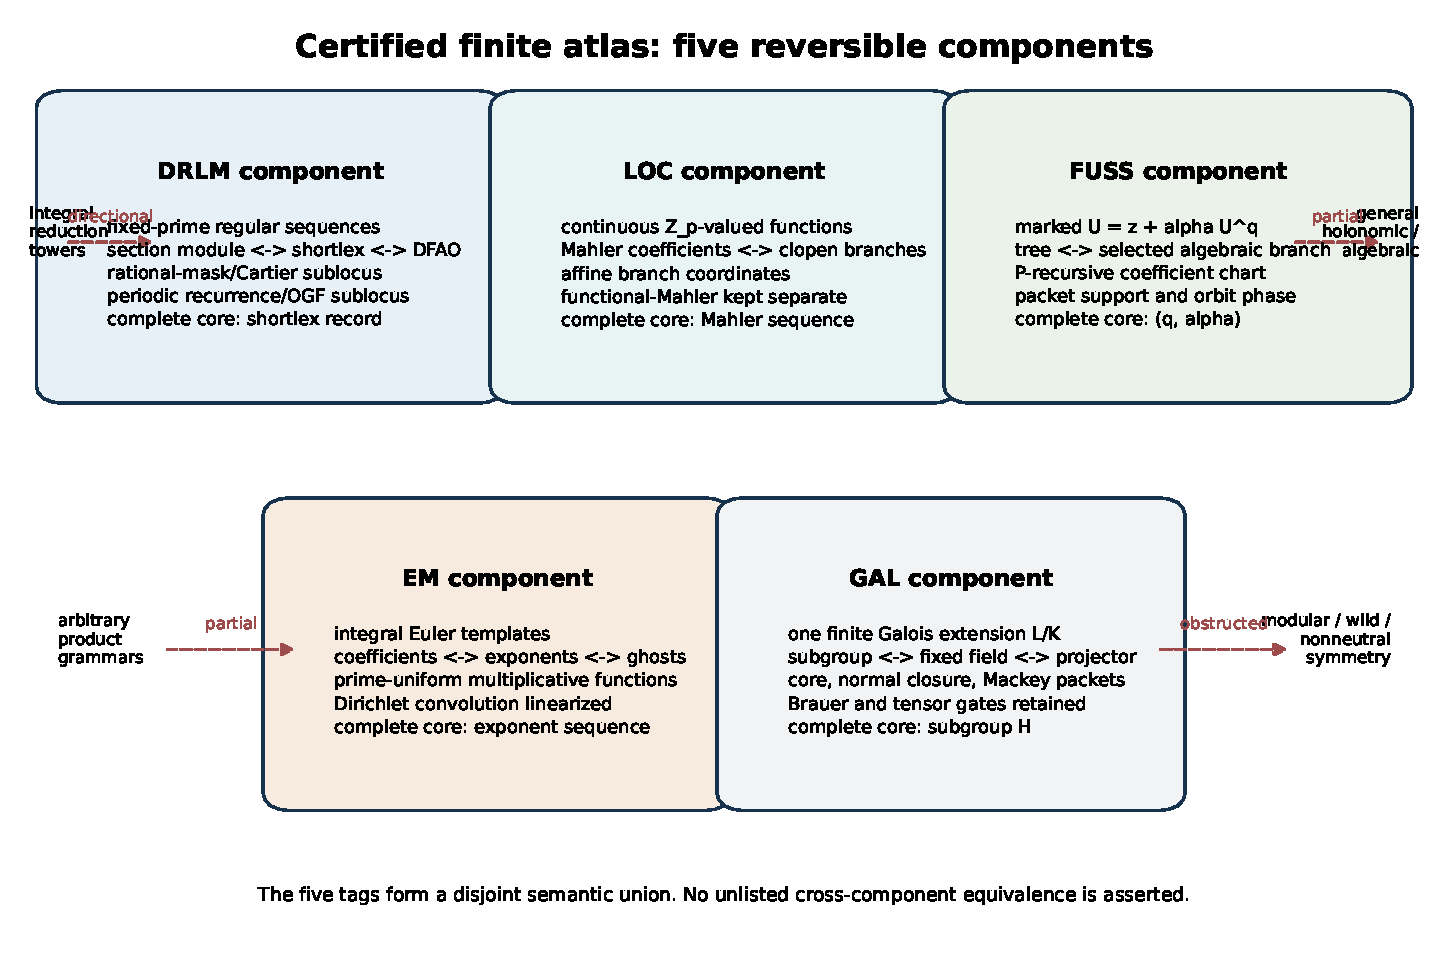
\includegraphics[width=.99\textwidth]{global_certified_atlas.pdf}
\caption{The certified finite atlas.  Each box is a nontrivial connected system of normalized charts.  Dashed external arrows are directional, partial, or obstructed satellites and are not promoted to equivalences.}
\label{fig:block13-certified-atlas}
\end{figure}

The semantic category of the total atlas is
\[
 \mathcal O_{13}
 =
 \mathcal O_{\mathrm{DRLM}}
 \sqcup
 \mathcal O_{\mathrm{Loc}}
 \sqcup
 \mathcal O_{\mathrm{Fuss}}
 \sqcup
 \mathcal O_{\mathrm{EM}}
 \sqcup
 \mathcal O_{\mathrm{Gal}}.
\]
The coproduct symbol is literal.  It does not assert that a finite-field regular sequence, a continuous \(p\)-adic function, a characteristic-zero marked tree branch, an integral Euler template, and a finite Galois subgroup are objects of one untyped category.  The tag records which semantic doctrine is in force.

\subsection{Normalizer-induced higher coherence}
\label{subsec:block13-normalizer-coherence}

Every connected component in \cref{def:block13-certified-atlas} has a canonical semantic normalizer.  For a chart \(\mathcal C_{\lambda,a}\) in component \(\lambda\), write
\[
 N_{\lambda,a}:\mathcal C_{\lambda,a}\longrightarrow\mathcal O_\lambda
\]
for the semantic normalization functor and choose its canonical inverse chart
\[
 Q_{\lambda,a}:\mathcal O_\lambda\longrightarrow\mathcal C_{\lambda,a}.
\]
The certified bridge from chart \(a\) to chart \(b\) is
\[
 \Phi_{ab}=Q_{\lambda,b}N_{\lambda,a}.
\]

\begin{theorem}[Normalizer-induced coherence]
\label{thm:block13-normalizer-coherence}
Assume that every normalized fiber of \(N_{\lambda,a}\) is contractible.  Then the comparison isomorphism
\[
 \eta_{abc}:
 \Phi_{bc}\Phi_{ab}
 \Longrightarrow
 \Phi_{ac}
\]
is unique.  Every triple-overlap diagram commutes, every quadruple-overlap coherence equation holds, and the composite around every finite bridge cycle is the identity transformation of the normalized chart.
\end{theorem}

\begin{proof}
Both \(\Phi_{bc}\Phi_{ab}(X)\) and \(\Phi_{ac}(X)\) are normalized presentations of the same semantic object \(N_{\lambda,a}(X)\).  Contractibility of the normalized fiber gives a unique isomorphism between them.  Any two composites occurring in a coherence diagram are isomorphisms between the same two normalized presentations, so uniqueness makes them equal.  The cycle statement follows by applying the same argument to the starting chart and itself.
\end{proof}

\begin{figure}[htbp]
\centering
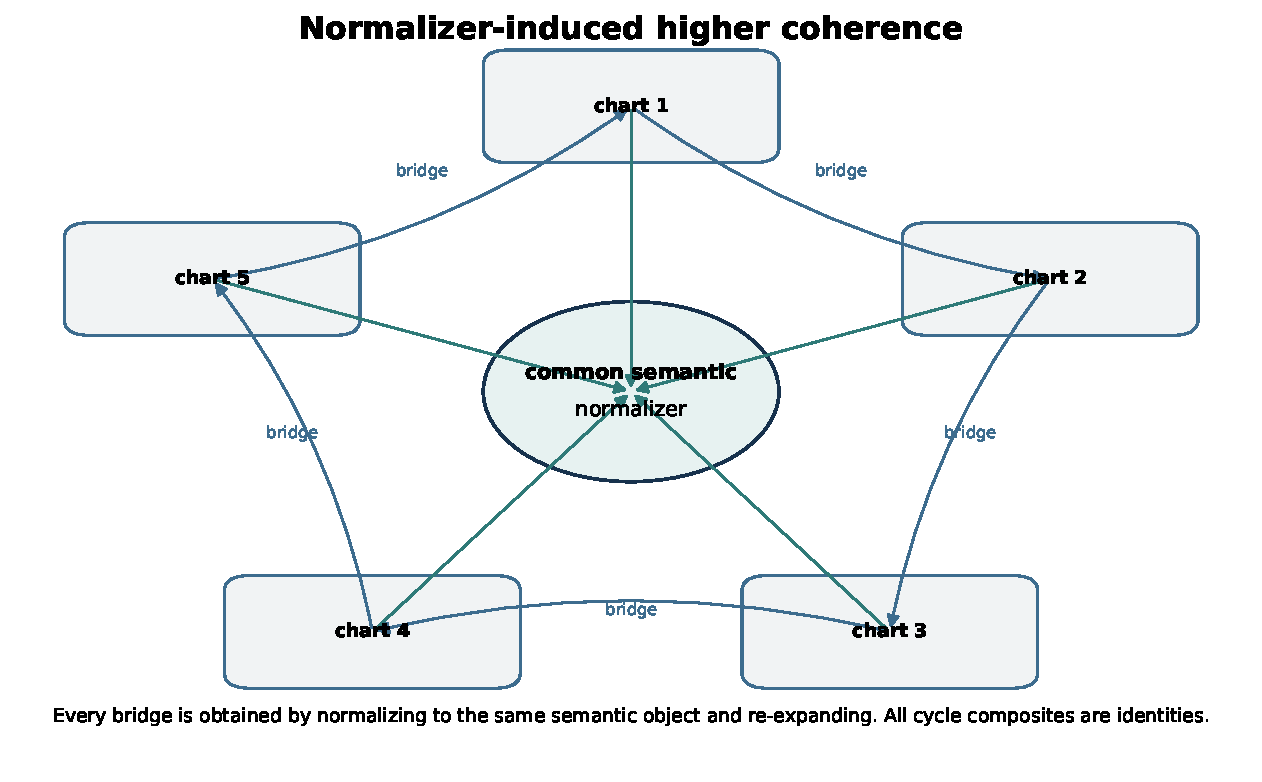
\includegraphics[width=.93\textwidth]{normalizer_induced_coherence.pdf}
\caption{Every reversible chart in one certified component normalizes to the same semantic object.  The unique normalized comparison forces all finite bridge cycles to commute.}
\label{fig:block13-normalizer-coherence}
\end{figure}

This theorem is not a substitute for constructing the normalizer.  It applies here because the preceding sections have already supplied unique reduced masks, reachable-observable Cartier modules, minimal automata, canonical section modules, marked fixed-point systems, selected algebraic branches, fixed Euler exponents, prime-power local factors, fixed subgroups, fixed fields, and faithful Reynolds projectors on the declared domains.

\subsection{Invariant descent theorem}
\label{subsec:block13-invariant-descent}

For every chart \(\mathcal C_{\lambda,a}\), let
\[
 I_{\lambda,a}:\mathcal C_{\lambda,a}\longrightarrow\mathcal V_{\lambda,a}
\]
be its native normalized invariant.  A bridge comparison is a natural isomorphism
\[
 \kappa_{ab}:
 J_{ab}I_{\lambda,a}
 \Longrightarrow
 I_{\lambda,b}\Phi_{ab},
\]
where \(J_{ab}\) transports invariant coordinates between their chart-specific target categories.

\begin{definition}[Coherent invariant family]
The family \((I_{\lambda,a},\kappa_{ab})\) is coherent when the two induced comparison maps from \(a\) to \(c\) agree on every triple overlap and the corresponding quadruple-overlap equation holds.
\end{definition}

\begin{theorem}[Certified finite invariant descent]
\label{thm:block13-certified-invariant-descent}
Let \(\mathfrak A_{13}\) be the atlas of \cref{def:block13-certified-atlas}.  Suppose that, in every connected component:
\begin{enumerate}
\item the local invariant is complete on every normalized chart;
\item the bridge comparisons are coherent;
\item invariant-compatible local isomorphisms satisfy effective descent.
\end{enumerate}
Then the local invariants induce a functor
\[
 \mathcal I_{13}:
 \Desc(\mathfrak A_{13})
 \longrightarrow
 \Desc(\mathfrak V_{13})
\]
that reflects isomorphisms.  If each semantic component is discrete, equality of descended invariants is equivalent to equality of the represented semantic objects.
\end{theorem}

\begin{proof}
The local comparison maps form a pseudonatural invariant family, so \cref{thm:atlas-assembly} gives the descended functor.  Equality or isomorphism of the descended invariant gives compatible local invariant matches.  Local completeness supplies local object isomorphisms.  Effective isomorphism descent glues those local isomorphisms to an isomorphism in the descent category.  On a discrete semantic component, every isomorphism is equality.
\end{proof}

\begin{figure}[htbp]
\centering
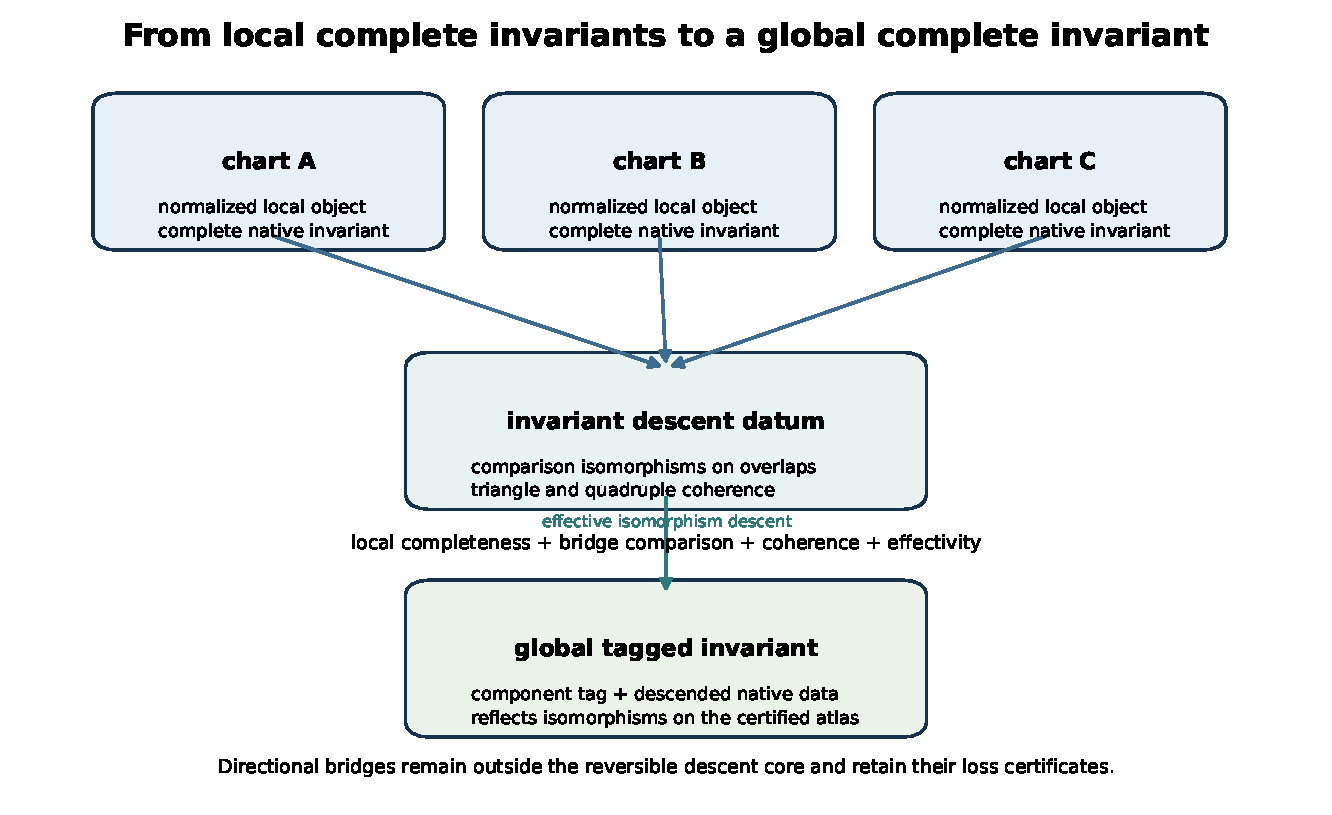
\includegraphics[width=.95\textwidth]{global_invariant_descent.pdf}
\caption{The global invariant theorem has four separate requirements.  Local completeness alone is insufficient without comparison maps, higher coherence, and effective descent of the resulting isomorphisms.}
\label{fig:block13-invariant-descent}
\end{figure}

\subsection{Digital--regular--linear--functional-Mahler component}
\label{subsec:block13-drlm}

Fix the prime \(p\) and let
\[
 \mathcal O_{\mathrm{DRLM}}
 =\mathbf{Reg}_p(\mathbb F_p)
\]
be the discrete semantic category of \(p\)-regular sequences over \(\mathbb F_p\).  By the finite-field fixed-radix theorem, every object is also \(p\)-automatic.  Its globally defined normalized charts are the canonical section module, the strict shortlex pointed digit-linear record, and the minimal least-significant-digit-first \(p\)-DFAO.

Two full replete subcategories carry additional charts.
\begin{enumerate}
\item On the rational-mask locus \(\RMah_p^{\times}\), the reduced functional-Mahler mask and the minimal reachable-observable Cartier module are equivalent to the digital charts.
\item On the unit purely periodic locus, the minimal recurrence, reduced rational OGF, minimal finite linear state, primitive period word, and rational-mask chart are all equivalent.
\end{enumerate}

For \(a\in\mathcal O_{\mathrm{DRLM}}\), define
\[
 \mathcal J_{\mathrm{DRLM},p}(a)
 =
 \left(
 \mathsf{SL}_{p,\mathbb F_p}(a),
 \mathcal P_{\mathrm{rm}}(a),
 \mathcal P_{\mathrm{per}}(a)
 \right),
\]
where \(\mathsf{SL}_{p,\mathbb F_p}(a)\) is the strict shortlex record, \(\mathcal P_{\mathrm{rm}}(a)\) is empty off the rational-mask locus and otherwise contains the reduced mask, Cartier module, collapse obstruction, and minimal automaton coordinates, and \(\mathcal P_{\mathrm{per}}(a)\) is empty off the purely periodic locus and otherwise contains the primitive period word, exact period, minimal recurrence, reduced OGF, and periodic packet profile.

\begin{theorem}[Digital--regular--linear--Mahler comparison theorem]
\label{thm:block13-drlm-comparison}
The invariant \(\mathcal J_{\mathrm{DRLM},p}\) is preserved by every reversible bridge in \(\mathfrak A_{\mathrm{DRLM},p}\).  Its comparison cells satisfy all higher coherence equations.  The strict shortlex coordinate reconstructs the represented regular sequence, so the descended invariant is complete on \(\mathbf{Reg}_p(\mathbb F_p)\).  The mask and periodic packages are compatible exact refinements on their respective subloci.
\end{theorem}

\begin{proof}
The canonical section module, strict shortlex record, and minimal orbit automaton normalize to the same coefficient sequence by the Fixed-radix regular atlas effective-descent theorem.  On the rational-mask locus, fixed-denominator Cartier intertwining identifies the reachable numerator span with the canonical section module and the reachable numerator set with the minimal automaton states.  On the periodic locus, the recurrence, rational, state, automaton, and mask charts normalize to the same primitive coefficient word.  Every comparison therefore factors through the same semantic normalizer, and \cref{thm:block13-normalizer-coherence} applies.  Completeness follows from the strict shortlex reconstruction formula.
\end{proof}

\begin{table}[htbp]
\centering
\caption{Representative cross-stratum invariant comparisons.}
\label{tab:block13-examples}
\scriptsize
\begin{tabularx}{\textwidth}{@{}L{0.15\textwidth}L{0.12\textwidth}L{0.13\textwidth}L{0.13\textwidth}L{0.13\textwidth}Y@{}}
\toprule
Example & Period & Recurrence order & Regular rank & DFAO states & Mask compiler degree\\
\midrule
$\mathbb {F}_2$/ word 10 & 2 & 2 & 2 & 3 & 2\\
$\mathbb {F}_2$/ word 110 & 3 & 2 & 2 & 3 & 2\\
$\mathbb {F}_3$/ word 12 & 2 & 1 & 1 & 2 & 1\\
\bottomrule
\end{tabularx}
\end{table}


The table gives representative objects for which recurrence order, regular rank, automaton size, and mask-compiler dimension are different coordinates of the same normalized semantic sequence.  Equality of one displayed scalar alone is not a complete invariant; the complete records are the chart objects described above.

The inclusions of the rational-mask and periodic loci are not essentially surjective.  Over a finite field every regular sequence is automatic, but many automatic sequences have no rational canonical mask, and many rational-mask sequences are not periodic.  The optional fields in \(\mathcal J_{\mathrm{DRLM},p}\) record these exact domain boundaries rather than forcing one chart to exist everywhere.

\subsection{Continuous Newton--Mahler component}
\label{subsec:block13-loc}

Let
\[
 \mathcal O_{\mathrm{Loc}}
 =C(\mathbb Z_p,\mathbb Z_p)
\]
with equality morphisms.  Its canonical coordinate is the Mahler sequence
\[
 \mathcal M_p(f)
 =
 (c_r(f))_{r\ge0},
 \qquad
 c_r(f)=\Delta^r f(0),
 \qquad
 c_r(f)\longrightarrow0.
\]
At every declared depth \(p^a\), the complete clopen branch packet
\[
 \bigl(f(p^aq+s)\bigr)_{0\le s<p^a}
\]
and the corresponding branchwise Mahler coefficients are reversible by explicit piecewise synthesis.  Affine branch kernels and mixed-radix refinements are comparison charts of the same semantic function.

\begin{theorem}[Continuous local invariant comparison]
\label{thm:block13-local-comparison}
The Mahler coefficient sequence
\[
 \mathcal J_{\mathrm{Loc},p}(f)
 =
 (c_r(f))_{r\ge0}
\]
is a complete invariant of \(\mathfrak A_{\mathrm{Loc},p}\).  Complete branch packets, branchwise Mahler coordinates, affine coefficient kernels, and nested refinements admit coherent comparison maps to \(\mathcal J_{\mathrm{Loc},p}\).
\end{theorem}

\begin{proof}
Mahler analysis and synthesis are mutually inverse on \(C(\mathbb Z_p,\mathbb Z_p)\).  Complete clopen analysis and piecewise synthesis are mutually inverse at each depth, and the nested branch law is strict.  Conjugating those maps by Mahler analysis gives the affine coefficient comparisons, whose mixed-radix composition was proved in Local Mahler-polyphase atlas.  All normalized charts therefore return the same function and the same Mahler sequence, so \cref{thm:block13-normalizer-coherence} gives higher coherence.
\end{proof}

Functional-Mahler equations for coefficient series are not included in this component.  A finite-state or functional-Mahler object enters the Newton--Mahler component only through a separately declared lift and interpolation constructor carrying its own precision and information-loss certificate.

\subsection{A genuine nonlinear--algebraic--holonomic overlap}
\label{subsec:block13-fuss}

Let \(K\) be a characteristic-zero field.  For an integer \(q\geq2\) and \(\alpha\in K^\times\), let
\[
 U_{q,\alpha}(z)\in zK[[z]]
\]
be the unique selected branch satisfying
\begin{equation}
 U=z+\alpha U^q.
 \label{eq:block13-fuss-tree}
\end{equation}
The derivative of
\[
 P_{q,\alpha}(z,Y)=Y-z-\alpha Y^q
\]
with respect to \(Y\) is one at \((0,0)\), so the branch is simple and selected by \(U(0)=0\).

Put
\[
 x=z^{q-1},
 \qquad
 U_{q,\alpha}(z)=zC_{q,\alpha}(x).
\]
Then
\begin{equation}
 C=1+\alpha xC^q.
 \label{eq:block13-fuss-compressed}
\end{equation}
Lagrange inversion gives
\begin{equation}
 [x^n]C_{q,\alpha}(x)
 =
 c_n(q,\alpha)
 =
 \frac{\alpha^n}{(q-1)n+1}
 \binom{qn}{n}.
 \label{eq:block13-fuss-coefficients}
\end{equation}
Define
\[
 A_q(n)
 =(n+1)\prod_{r=2}^{q}\bigl((q-1)n+r\bigr),
\]
\[
 B_q(n)
 =\prod_{r=1}^{q}(qn+r).
\]
Then the coefficient sequence satisfies the first-order polynomial recurrence
\begin{equation}
 \boxed{
 A_q(n)c_{n+1}
 =
 \alpha B_q(n)c_n.}
 \label{eq:block13-fuss-recurrence}
\end{equation}
After dividing the polynomial gcd of \(A_q\) and \(B_q\), this is the normalized first-order tail recurrence with initial value \(c_0=1\).

\begin{theorem}[Fuss--Catalan three-stratum equivalence]
\label{thm:block13-fuss-equivalence}
The following normalized marked presentations determine one another exactly:
\begin{enumerate}
\item the polynomial tree system \(U=z+\alpha U^q\);
\item the selected algebraic branch \((P_{q,\alpha},U(0)=0)\);
\item the compressed P-recursive coefficient chart \((\cref{eq:block13-fuss-recurrence},c_0=1)\) together with the support embedding \(U(z)=zC(z^{q-1})\).
\end{enumerate}
Every normalized fiber is contractible.  All triangle comparisons return the same parameter pair \((q,\alpha)\).
\end{theorem}

\begin{proof}
The marked tree equation is the selected algebraic equation.  Simplicity at the origin gives its unique formal branch.  Substitution \(U=zC(z^{q-1})\) gives \cref{eq:block13-fuss-compressed}.  Lagrange inversion gives \cref{eq:block13-fuss-coefficients}, and taking the ratio of consecutive coefficients gives \cref{eq:block13-fuss-recurrence}.  Conversely, the recurrence and initial value reconstruct \(C\), the support embedding reconstructs \(U\), and the reconstructed series satisfies the selected algebraic equation.  A normalized automorphism fixes \(q\), \(\alpha\), and the unique branch, hence is the identity.
\end{proof}

\begin{figure}[htbp]
\centering
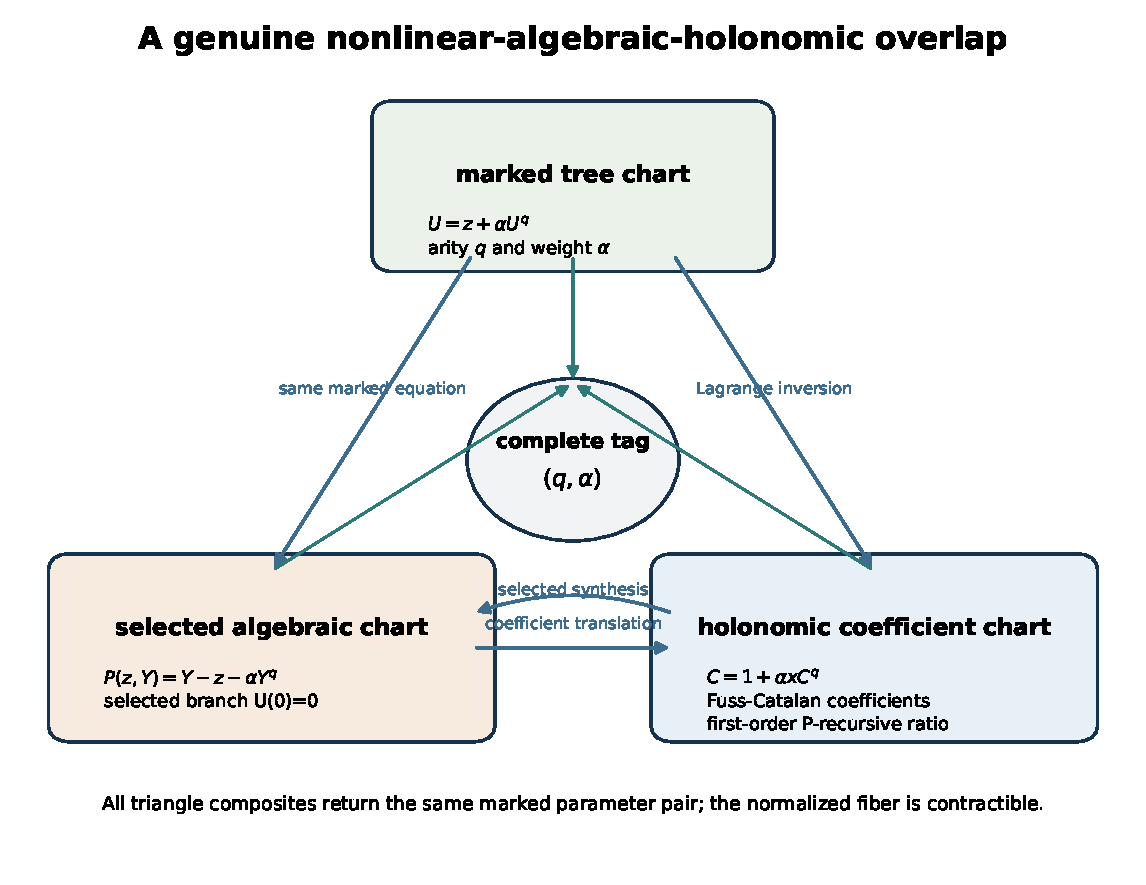
\includegraphics[width=.87\textwidth]{fuss_catalan_three_stratum.pdf}
\caption{The marked Fuss--Catalan family gives a genuine overlap among the nonlinear tree, selected algebraic, and holonomic recurrence strata.  Every path returns the same marked pair \((q,\alpha)\).}
\label{fig:block13-fuss-triangle}
\end{figure}

The tree arity period is \(q-1\).  For packet modulus \(N\), set
\[
 g_N=\gcd(N,q-1).
\]
The nonzero coefficient addresses of \(U_{q,\alpha}\) are exactly
\[
 j\equiv1\pmod{g_N},
\]
and the complete dominant singularity orbit has size
\[
 \frac{q-1}{g_N}
\]
under the positive analytic hypotheses of \cref{thm:block11-qary-phase}.  These packet signatures agree in the tree and algebraic charts because both are computed from the same selected branch.

Define
\[
 \mathcal J_{\mathrm{Fuss}}(q,\alpha)
 =
 \left(
 q,
 \alpha,
 P_{q,\alpha},
 \{c_n(q,\alpha)\}_{n\geq0},
 \{g_N\}_{N\geq1},
 \left\{\frac{q-1}{g_N}\right\}_{N\geq1}
 \right).
\]

\begin{corollary}[Complete cross-stratum invariant on the marked Fuss family]
\label{cor:block13-fuss-invariant}
The nonlinear, algebraic, holonomic, packet-support, and dominant-orbit invariants admit coherent comparison maps to \(\mathcal J_{\mathrm{Fuss}}\).  The package is complete on the declared marked family.
\end{corollary}

\begin{proof}
Coherence follows from \cref{thm:block13-fuss-equivalence,thm:block13-normalizer-coherence}.  The first two entries reconstruct the marked fixed-point equation and therefore its unique selected branch.
\end{proof}

\begin{table}[htbp]
\centering
\caption{Named weighted q-ary examples in the cross-stratum atlas.}
\label{tab:block13-qary-examples}
\scriptsize
\begin{tabularx}{\textwidth}{@{}L{0.10\textwidth}L{0.11\textwidth}L{0.12\textwidth}L{0.25\textwidth}L{0.17\textwidth}Y@{}}
\toprule
$q$ & $\lambda$ & Support period & First supported coefficients & Active addresses at $N=6$ & Packet-orbit size\\
\midrule
2 & $1$ & 1 & $(1, 1, 2, 5,\ldots)$ & $\{0,1,2,3,4,5\}$ & 1\\
3 & $2$ & 2 & $(1, 2, 12, 96,\ldots)$ & $\{1,3,5\}$ & 1\\
4 & $-1$ & 3 & $(1, -1, 4, -22,\ldots)$ & $\{1,4\}$ & 1\\
5 & $1/2$ & 4 & $(1, 1/2, 5/4, 35/8,\ldots)$ & $\{1,3,5\}$ & 2\\
\bottomrule
\end{tabularx}
\end{table}


The examples show that the finite invariant retains the weight parameter as well as the arity.  Support period alone recovers only \(q-1\); the coefficient \([z^q]U=\alpha\) supplies the second coordinate.

This is not a classification of arbitrary algebraic branches, arbitrary P-recursive sequences, or unmarked nonlinear fixed points.  It is the first explicit complete invariant on a connected overlap of those three strata.

\subsection{Euler--multiplicative component}
\label{subsec:block13-em}

Let
\[
 A_b(z)=\prod_{m\geq1}(1-z^m)^{-b_m}
\]
be an integral unit series in the fixed Euler basis, and let
\[
 c_n=\sum_{d\mid n}d\,b_d
\]
be its divisor-ghost sequence.  Define the prime-uniform multiplicative function
\[
 f_b(n)=\prod_{p^e\parallel n}[z^e]A_b(z).
\]
Every prime has the same local factor \(A_b(T)\).  By \cref{thm:block07-euler-classification,thm:block07-product-multiplicative-descent}, the coefficient, exponent, ghost, and prime-uniform multiplicative charts are reversible on this declared locus.

\begin{theorem}[Euler--multiplicative invariant comparison]
\label{thm:block13-em-comparison}
The exponent sequence
\[
 \mathcal J_{\mathrm{EM}}(A_b)=b
\]
is a complete invariant of the certified Euler--multiplicative component.  In every chart it is recovered by the same M\"obius formula
\[
 b_n
 =
 \frac1n
 \sum_{d\mid n}\mu(n/d)c_d,
\]
and Dirichlet convolution corresponds to exponent addition.
\end{theorem}

\begin{proof}
Unique Euler factorization reconstructs \(A_b\) from \(b\).  Prime-power reconstruction then reconstructs \(f_b\).  The logarithmic-derivative identity gives \(c\), and M\"obius inversion recovers \(b\).  Every bridge therefore factors through the same exponent normalizer, so higher coherence follows from \cref{thm:block13-normalizer-coherence}.
\end{proof}

The theorem remains confined to the fixed Euler basis and the prime-uniform multiplicative essential image.  It does not identify arbitrary Cauchy-product grammars with arbitrary Dirichlet-convolution systems.

\subsection{Finite Galois component}
\label{subsec:block13-gal}

Fix a finite Galois extension \(L/K\) in the semisimple setting.  For each subgroup \(H\leq G\), define
\[
 \mathcal J_{\mathrm{Gal}}(H)
 =
 \left(
 H,
 L^H,
 P_H,
 \operatorname{Core}_G(H),
 \operatorname{Ncl}_G(H),
 \{J\backslash G/H\}_{J\leq G}
 \right).
\]

\begin{theorem}[Finite Galois invariant comparison]
\label{thm:block13-gal-comparison}
The subgroup, fixed-field, and faithful Reynolds-projector charts have coherent comparison maps to \(\mathcal J_{\mathrm{Gal}}\).  The invariant is complete on the normalized subgroup atlas for the fixed extension \(L/K\).
\end{theorem}

\begin{proof}
The first three entries determine one another by \cref{thm:block12-normalized-galois-chart}.  Core, normal closure, and double-coset packets are functorial constructions from the subgroup.  The subgroup coordinate itself is complete, and the strict subgroup normalizer forces coherence.
\end{proof}

The Brauer class and Tannakian group scheme are not added to this complete subgroup invariant as if they were automatic coordinates.  They belong to separately typed projective and tensor extensions whose hypotheses and obstructions were stated in Galois-Tannakian atlas.

\subsection{The global tagged invariant}
\label{subsec:block13-global-tagged}

Let
\[
 \Lambda_{13}
 =
 \{\mathrm{DRLM},\mathrm{Loc},\mathrm{Fuss},\mathrm{EM},\mathrm{Gal}\}
\]
be the component-tag set.  Define
\[
 \mathcal J_{13}(X)
 =
 \bigl(\lambda(X),\mathcal J_{\lambda(X)}(X)\bigr).
\]

\begin{theorem}[Certified global completeness theorem]
\label{thm:block13-global-completeness}
The invariant \(\mathcal J_{13}\) descends across every reversible bridge in \(\mathfrak A_{13}\) and is complete on
\[
 \mathcal O_{13}
 =
 \mathcal O_{\mathrm{DRLM}}
 \sqcup
 \mathcal O_{\mathrm{Loc}}
 \sqcup
 \mathcal O_{\mathrm{Fuss}}
 \sqcup
 \mathcal O_{\mathrm{EM}}
 \sqcup
 \mathcal O_{\mathrm{Gal}}.
\]
More precisely,
\[
 \boxed{
 \mathcal J_{13}(X)=\mathcal J_{13}(Y)
 \quad\Longleftrightarrow\quad
 X=Y
 }
\]
inside the declared discrete semantic category.  The associated invariant functor reflects isomorphisms on the descent category.
\end{theorem}

\begin{proof}
Within each component, completeness is \cref{thm:block13-drlm-comparison,thm:block13-local-comparison,cor:block13-fuss-invariant,thm:block13-em-comparison,thm:block13-gal-comparison}.  Their comparison maps are coherent by \cref{thm:block13-normalizer-coherence}.  The component tag prevents an object in one semantic doctrine from being identified with an object in another.  Apply \cref{thm:block13-certified-invariant-descent} componentwise and then take the finite coproduct.
\end{proof}

\begin{remark}[What is genuinely global]
The theorem is not the tautology that every object is classified by itself.  Each component invariant is computed in one native chart and transported through several nonidentical presentation categories.  The global assertion is that these transported coordinates agree coherently and classify the descent object.  The coproduct tag is nevertheless essential: the current Library does not provide reversible bridges joining all five components.
\end{remark}

\subsection{Directional satellites and exact loss records}
\label{subsec:block13-directional-satellites}

The certified reversible core is surrounded by directional bridges that remain useful for theorem transport and computation.  Their failure to enter \(\mathcal J_{13}\) is controlled by explicit loss data.

\begin{table}[htbp]
\centering
\caption{Directional satellites of the certified global invariant atlas.}
\label{tab:block13-directional-satellites}
\small
\begin{tabularx}{\textwidth}{@{}L{0.23\textwidth}L{0.19\textwidth}Y@{}}
\toprule
Directional bridge & Retained structure & Exact loss or obstruction\\
\midrule
Integral regular lattice \(\to\) residue section module & digit transitions and residue semantics & Smith--Tor ghost kernel and missing quotient\\
General regular sequence \(\dashrightarrow\) rational mask & coefficient semantics on the essential image & rational-mask existence and collapse obstruction\\
Algebraic branch \(\to\) holonomic annihilator & D-finite coefficient semantics & selected branch and minimal polynomial may be forgotten\\
Marked nonlinear system \(\to\) semantic fixed point & the represented fixed point & generator labels, arities, and tree grammar may be forgotten\\
Finite-state dynamics \(\to\) Newton--Mahler chart & congruence branch values and precision ladder & depends on a chosen lift and principal-unit hypothesis\\
Projective Galois cocycle \(\dashrightarrow\) linear descent & projective action & relative Brauer class\\
Faithful corner realization \(\dashrightarrow\) Tannakian symmetry & additive packet and operator equations & exact tensor, dual, unit, and fiber-functor data are absent\\
\bottomrule
\end{tabularx}
\end{table}

\begin{proposition}[No completeness transport through an unreflected directional bridge]
\label{prop:block13-no-directional-completeness}
Let \(T:\mathcal C\to\mathcal D\) be a directional bridge.  A complete invariant on \(\mathcal D\) pulls back to a complete invariant on \(\mathcal C\) only if \(T\) reflects isomorphisms on the declared source subcategory.  In particular, any nontrivial object-collapse relation or obstruction fiber prevents automatic completeness transport.
\end{proposition}

\begin{proof}
If \(T\) does not reflect isomorphisms, there exist nonisomorphic \(X,Y\) with \(T(X)\cong T(Y)\).  Every invariant depending only on the target object then takes the same value on \(X\) and \(Y\), so its pullback cannot be complete.
\end{proof}

\subsection{Exact finite verification}
\label{subsec:block13-verification}

Two complementary exact suites audit Global synthesis atlas.  The first authenticates the frozen preceding verification records and checks the broad bridge matrix, periodic and product--multiplicative overlap replays, directional-loss controls, finite \v{C}ech holonomy models, and the five completeness gates.  The second checks the weighted \(q\)-ary tree--algebraic--holonomic overlap, its coefficient and packet equations, parameter recovery, detailed bridge ledger, and tagged component separation.

\begin{table}[htbp]
\centering
\caption{Exact verification of the Global synthesis atlas invariant-descent and weighted q-ary cross-stratum models.}
\label{tab:block13-global-invariant-validation}
\small
\begin{tabularx}{\textwidth}{@{}Y r@{}}
\toprule
Validation class & Checks\\
\midrule
Bridge-matrix structural checks & 172\\
Weighted q-ary coefficient identities & 1,856\\
Exact support-period identities & 8,192\\
Formal fixed-point identities & 8,192\\
Minimal-polynomial relation checks & 8,192\\
Finite parameter recovery & 128\\
Tree/algebraic/holonomic comparison paths & 64\\
Supported first-order recurrence checks & 1,792\\
Packet support and orbit-phase checks & 2,112\\
Exact packet synthesis checks & 44,352\\
Address-carry packet equations & 44,352\\
Tagged component-separation checks & 49\\
\midrule
\textbf{Global synthesis exact checks} & \textbf{119,453}\\
\textbf{Failures} & \textbf{0}\\
\bottomrule
\end{tabularx}
\end{table}


\begin{table}[htbp]
\centering
\caption{Exact verification of the Global synthesis atlas global-invariant and cross-stratum synthesis layer.}
\label{tab:block13-combined-validation}
\small
\begin{tabularx}{\textwidth}{@{}Y r@{}}
\toprule
Validation suite & Exact assertions\\
\midrule
Bridge matrix, overlap replay, directional-loss, and finite \v{C}ech suite & 154,209\\
Weighted $q$-ary tree--algebraic--holonomic and tagged-invariant suite & 119,453\\
\midrule
Regression/authentication assertions already represented in the certified native-stratum program & 39,846\\
\textbf{New Global synthesis atlas comparison and coherence assertions} & \textbf{233,816}\\
All assertions executed by the two Global synthesis atlas suites & 273,662\\
Failures & 0\\
\bottomrule
\end{tabularx}
\end{table}


The two suites execute \(\BlockThirteenChecks\) exact assertions with no failures.  Of these, \(\BlockThirteenRegressionChecks\) authenticate or replay assertions already represented in the preceding cumulative record.  The global synthesis therefore contributes \(\BlockThirteenNewChecks\) nonduplicative comparison, coherence, packet, and loss-control assertions.  The blockwise cumulative record is
\[
 \boxed{\BlockThirteenCumulative}
\]
exact assertions with no recorded failures.  Counting every regression assertion executed during the Global synthesis atlas replay gives \(\BlockThirteenCumulativeExecuted\) total executed assertions.  Neither number is a count of independent theorems.

The bridge-synthesis suite replays primitive unit-periodic words over finite prime fields, compares their recurrence, OGF, automaton, section-module, and functional-Mahler coordinates, verifies the prime-uniform Euler--multiplicative overlap, and tests finite nontrivial \v{C}ech cycle models.  The weighted \(q\)-ary suite checks the fixed-point identity, Lagrange coefficients, first-order P-recursive recurrence, support phases, exact packet synthesis, address-carry equations, and all triangle normalizers over a declared finite parameter grid.  Both machine-readable records are included in the source package.

\begin{boundarybox}
\textbf{Exact boundary of Global synthesis atlas.}
The global invariant theorem is proved for the five-component certified finite atlas in \cref{def:block13-certified-atlas}.  It does not assert a complete invariant for every object in the eight broad strata, a reversible bridge between the five semantic components, effective descent for every directional satellite, cross-radix or all-ring normalization, modular or wild Galois effectivity, nonneutral Tannakian reconstruction, or classification of unmarked general holonomic, algebraic, and nonlinear systems.
\end{boundarybox}

\begin{resultbox}
\textbf{Section result.}
The manuscript now contains an authoritative broad-stratum bridge matrix, a finite certified atlas with five nontrivial connected components, explicit invariant comparison maps, a normalizer-induced higher-coherence theorem, and a complete tagged global invariant on the declared semantic union.  The new Fuss--Catalan triangle gives a genuine nonlinear--algebraic--holonomic overlap.  The digital--regular--functional-Mahler, continuous Newton--Mahler, Euler--multiplicative, and finite Galois components consolidate the exact cross-presentation results of the preceding stratum sections without conflating the two Mahler theories.  Directional bridges remain outside the reversible core and retain their precise loss or obstruction records.  This closes the finite global-invariant milestone on a substantial atlas, not the unrestricted eight-stratum stack.
\end{resultbox}


\clearpage
\section{Universal lane transport at finite profile}
\label{sec:block15-universal-lane-transport}

The preceding parts of the manuscript establish packet coordinates in an
additive idempotent-complete setting and verify them separately in several
native strata.  This section isolates the common finite theorem.  The word
``lane'' will mean a packet together with its address, its chosen splitting,
and its position in a declared refinement system.  Thus a lane is more than a
subsequence or a suggestive decomposition.  It carries the exact data needed
for analysis, synthesis, transfer, refinement, and reconstruction.

The theorem is universal only in a profiled sense.  Its algebraic core applies
to every additive realization that preserves the finite sums, compositions,
split idempotents, and refinement identities used in the proof.  Kernel,
quotient, tensor, topological, metric, and nonlinear conclusions require the
additional hypotheses stated where they occur.

\subsection{Finite profiled lane systems}
\label{subsec:block15-lane-systems}

\begin{definition}[Finite resolution shape]
\label{def:block15-resolution-diagram}
A finite resolution shape is a finite partially ordered set
\(\mathsf R\).  We write \(s\succeq r\) when \(s\) is finer than \(r\).
The shape contains no address sets: object-specific addresses and their
refinement maps are declared in the lane system below.
\end{definition}

\begin{definition}[Finite profiled lane system]
\label{def:block15-finite-profiled-lane-system}
Let \(\mathcal C\) be an additive idempotent-complete category, let
\(X\in\mathcal C\), and let \(\mathsf R\) be a finite resolution shape.  A
finite profiled lane system \(\mathcal L_X\) consists, for every
\(r\in\mathsf R\), of a finite address set \(I_{X,r}\) and a family
\[
 \mathcal P_X^r=(p_{X,i}^r)_{i\in I_{X,r}}
 \subseteq\End_{\mathcal C}(X)
\]
with
\[
 (p_{X,i}^r)^2=p_{X,i}^r,
 \qquad
 p_{X,i}^rp_{X,j}^r=0\quad(i\ne j),
 \qquad
 \sum_{i\in I_{X,r}}p_{X,i}^r=1_X,
\]
together with chosen splittings
\[
 X_i^r\xrightarrow{\iota_{X,i}^r}X
 \xrightarrow{\pi_{X,i}^r}X_i^r,
 \qquad
 \iota_{X,i}^r\pi_{X,i}^r=p_{X,i}^r,
 \qquad
 \pi_{X,i}^r\iota_{X,i}^r=1_{X_i^r}.
\]
For \(s\succeq r\), the system also contains a surjection
\[
 \rho^X_{sr}:I_{X,s}\twoheadrightarrow I_{X,r}
\]
such that
\[
 p_{X,i}^r
 =
 \sum_{\rho^X_{sr}(j)=i}p_{X,j}^s,
 \qquad
 \rho^X_{tr}=\rho^X_{sr}\rho^X_{ts}.
\]
Here \(\rho^X_{rr}=1_{I_{X,r}}\).  The address sets and refinement maps are
declared data; they are not inferred from their cardinalities.
Its verified profile contains finite biproducts, addition of morphisms,
composition, the displayed splittings, and these projector-sum refinement
identities.  Any further constructor is included only after its preservation
has been verified.
\end{definition}

At resolution \(r\), write
\[
 \Analysis_X^r
 :=(\pi_{X,i}^r)_i:
 X\longrightarrow\bigoplus_iX_i^r,
 \qquad
 \Synthesis_X^r
 :=(\iota_{X,i}^r)_i:
 \bigoplus_iX_i^r\longrightarrow X.
\]
For profiled lane systems on \(X\) and \(Y\), define the coordinate block of
\(f:X\to Y\) at resolutions \(r,u\) by
\[
 [f]^{u,r}_{a i}
 :=
 \pi_{Y,a}^u f\iota_{X,i}^r:
 X_i^r\longrightarrow Y_a^u.
\]
Its ambient corner is
\[
 p_{Y,a}^u f p_{X,i}^r
 =
 \iota_{Y,a}^u[f]^{u,r}_{a i}\pi_{X,i}^r.
\]

\subsection{The universal finite transport theorem}
\label{subsec:block15-main-theorem}

\begin{theorem}[Universal Lane Transport Theorem, finite profiled form]
\label{thm:block15-universal-lane-transport}
Let \(\mathcal C\) be an additive idempotent-complete category.  Give each of
the objects \(X_0,\ldots,X_m\) a finite profiled lane system.  Then all of the
following statements hold.

\begin{enumerate}[label=\textup{(L\arabic*)}]
\item \textbf{Exact analysis and synthesis.}  At every declared resolution,
\[
 \Synthesis_X^r\Analysis_X^r=1_X,
 \qquad
 \Analysis_X^r\Synthesis_X^r
 =1_{\oplus_iX_i^r}.
\]
Hence \(X\cong\bigoplus_iX_i^r\).

\item \textbf{Unique lane matrix.}  Every morphism \(f:X\to Y\) is recovered
uniquely from its lane blocks:
\[
 f
 =
 \sum_{a,i}p_{Y,a}^u f p_{X,i}^r
 =
 \sum_{a,i}\iota_{Y,a}^u
 [f]^{u,r}_{a i}\pi_{X,i}^r.
\]
Equivalently, the assignment
\[
 f\longmapsto
 \bigl([f]^{u,r}_{a i}\bigr)_{a,i}
\]
is a bijection from \(\Hom_{\mathcal C}(X,Y)\) to the group of rectangular
matrices with entries in
\(\Hom_{\mathcal C}(X_i^r,Y_a^u)\).

\item \textbf{Composition and path law.}  If \(f:X\to Y\) and \(g:Y\to Z\),
with the same resolution \(u\) used on the intermediate object, then
\[
 [gf]^{v,r}_{c i}
 =
 \sum_{a\in I_{Y,u}}[g]^{v,u}_{c a}[f]^{u,r}_{a i}.
\]
More generally, a block of a composable string is the finite sum of the
products along all compatible intermediate address paths.

\item \textbf{Projector-sum refinement.}  If \(s\succeq r\) on \(X\) and
\(v\succeq u\) on \(Y\), then
\[
 p_{Y,a}^u f p_{X,i}^r
 =
 \sum_{\rho^Y_{vu}(b)=a}
 \sum_{\rho^X_{sr}(j)=i}
 p_{Y,b}^v f p_{X,j}^s.
\]
Coarsening a fine composite gives the same ambient morphism as composing at
the coarse level.

\item \textbf{Selectors and named residuals.}  For
\(E\subseteq I_{Y,u}\times I_{X,r}\), put
\[
 C_E^{u,r}(f)
 :=\sum_{(a,i)\in E}p_{Y,a}^ufp_{X,i}^r,
 \qquad
 R_E^{u,r}(f):=f-C_E^{u,r}(f).
\]
As additive endomorphisms of \(\Hom_{\mathcal C}(X,Y)\),
\[
 C_E^2=C_E,
 \qquad
 C_EC_F=C_{E\cap F},
 \qquad
 R_E=1-C_E,
 \qquad
 f=C_E(f)+R_E(f).
\]
Thus deletion of a lane block is never silent.  Its complement is an exact,
named residual.

\item \textbf{Support transport.}  If \(f=C_E(f)\) and \(g=C_F(g)\), then
\[
 gf=C_{F\circ E}(gf),
\]
where \(F\circ E\) is relational composition through the intermediate
addresses.  For arbitrary \(f,g\), writing
\(f_E=C_E(f)\), \(r_f=R_E(f)\), \(g_F=C_F(g)\), and
\(r_g=R_F(g)\), one has the exact identity
\[
 gf-g_Ff_E
 =r_gf_E+g_Fr_f+r_gr_f.
\]

\item \textbf{Additive realization.}  Let
\(F:\mathcal C\to\mathcal D\) be an additive functor to another additive
idempotent-complete category.  If the verified profile of \(F\) contains the
chosen splittings and refinement identities, then
\[
 F([f]^{u,r}_{a i})
 =
 [F(f)]^{u,r}_{a i}
\]
after the declared splitting comparisons.  The functor carries analysis,
synthesis, matrix multiplication, projector-sum refinement, selectors, and
named residuals to their corresponding constructions in \(\mathcal D\).

\item \textbf{Exact fold loss.}  Let \(E\) be a finite set of retained lane
positions and set
\[
 B_e:=\Hom_{\mathcal C}(X_i^r,Y_a^u)
 \quad\text{for }e=(a,i)\in E.
\]
Let \(T\) be a finite set, let \(\kappa:E\to T\), let \(C_t\) be abelian
groups, and let \(\tau_e:B_e\to C_{\kappa(e)}\) be homomorphisms.  With
\(C=\bigoplus_{t\in T}C_t\) and coordinate inclusions
\(j_t:C_t\to C\), the fold
\[
 \Phi_{\kappa,\tau}:
 \bigoplus_{e\in E}B_e\longrightarrow C,
 \qquad
 (b_e)_e\longmapsto
 \sum_{e\in E}j_{\kappa(e)}\tau_e(b_e)
\]
has exact information-loss group \(\ker\Phi_{\kappa,\tau}\).  In particular,
two retained lane matrices have the same folded record exactly when their
difference belongs to this kernel.

Suppose, more strongly, that every \(\tau_e\) is injective and that there are
globally typed selectors \(Q_e\in\End(C)\) satisfying, for every
\(e,e'\in E\) and every \(b_{e'}\in B_{e'}\),
\[
 Q_ej_{\kappa(e')}\tau_{e'}(b_{e'})
 =
 \delta_{e,e'}j_{\kappa(e')}\tau_{e'}(b_{e'}).
\]
Then \(\Phi_{\kappa,\tau}\) is injective.  If there are also homomorphisms
\[
 r_e:C\longrightarrow B_e,
 \qquad
 r_ej_{\kappa(e)}\tau_e=1_{B_e},
\]
then
\[
 L:=\bigl(r_eQ_e\bigr)_{e\in E}:C\longrightarrow\bigoplus_{e\in E}B_e
\]
is a left inverse of \(\Phi_{\kappa,\tau}\), so the fold is split lossless.
\end{enumerate}
\end{theorem}

\begin{proof}
For (L1), the first composite is
\[
 \sum_i\iota_{X,i}^r\pi_{X,i}^r
 =\sum_i p_{X,i}^r=1_X.
\]
The \((i,j)\)-entry of the other composite is
\(\pi_{X,i}^r\iota_{X,j}^r\).  It is the identity when \(i=j\), and it is
zero otherwise because the corresponding idempotents annihilate one another.

For (L2), insert the two reconstruction identities on the two sides of
\(f\).  Applying \(\pi_{Y,a}^u\) on the left and
\(\iota_{X,i}^r\) on the right proves uniqueness of every entry.  For (L3),
insert
\(1_Y=\sum_a\iota_{Y,a}^u\pi_{Y,a}^u\) between \(g\) and \(f\).
Iteration gives the path formula.

For (L4), substitute the two projector-sum refinement identities into the
coarse ambient corner and distribute the finite sums.  The assertion about
composition follows from the same substitution at the intermediate object.

For (L5), each selector either fixes an ambient block or kills it.  Applying
two selectors therefore retains precisely the intersection.  The residual
identities follow by subtraction.  For (L6), expand each block of \(gf\)
through the intermediate resolution.  A surviving summand supplies an
intermediate address in the relational product.  The residual formula is the
finite expansion of
\((g_F+r_g)(f_E+r_f)-g_Ff_E\).

For (L7), additivity preserves zero maps and finite sums, functoriality
preserves identities and composition, and the splitting comparisons identify
the image of every source lane object with the declared target lane object.
The profile hypothesis is needed precisely for those identifications and for
the refinement equations.

For (L8), equality of two fold values is equivalent to the difference of the
two input families lying in the kernel.  Under the selector hypothesis, if
\(\Phi_{\kappa,\tau}((b_e)_e)=0\), applying \(Q_e\) gives
\(j_{\kappa(e)}\tau_e(b_e)=0\).  Both \(j_{\kappa(e)}\) and \(\tau_e\) are
injective, hence \(b_e=0\) for every \(e\).  The chosen retractions compose
with the \(Q_e\) to give the displayed left inverse: its \(e\)-coordinate
on the fold is \(r_eQ_ej_{\kappa(e)}\tau_e=1_{B_e}\), while strict
separation kills every other coordinate.
\end{proof}

\begin{remark}[Why the fold selectors live in one group]
\label{rem:block15-global-fold-typing}
The endomorphisms \(Q_e\) in (L8) all act on the single group
\(C=\bigoplus_tC_t\).  Writing separate selectors on unrelated codomains
would make the Kronecker relation ill-typed and would not prove injectivity of
the combined fold.
\end{remark}

\begin{proposition}[Exact visible-support loss ledger]
\label{prop:block15-visible-support-ledger}
Use the finite fold data of (L8) and fix an input family
\(b=(b_e)_{e\in E}\).  Define
\[
 S_0:=\{e\in E:b_e\ne0\},
 \qquad
 A_0:=\{e\in S_0:\tau_e(b_e)=0\},
 \qquad
 S_1:=S_0\setminus A_0,
\]
and let
\[
 \Gamma:=\kappa(S_1)\subseteq T.
\]
For \(t\in T\), write the folded coordinate as
\[
 \overline b_t
 :=
 \sum_{\substack{e\in S_1\\\kappa(e)=t}}\tau_e(b_e)
 \in C_t,
\]
and put
\[
 \operatorname{supp}(\overline b)
 :=\{t\in T:\overline b_t\ne0\},
 \qquad
 K_0:=\{t\in\Gamma:\overline b_t=0\}.
\]
Then
\[
 \boxed{
 |S_0|-|\operatorname{supp}(\overline b)|
 =
 |A_0|
 +\bigl(|S_1|-|\Gamma|\bigr)
 +|K_0|.}
\]
The three terms record, respectively, annihilation by the local maps
\(\tau_e\), collision of surviving lane addresses under \(\kappa\), and
cancellation among folded values at a common address.  If every \(\tau_e\) is
injective, then \(A_0=\varnothing\).  If globally typed selectors satisfy the
strict separation law of (L8), then \(K_0=\varnothing\).
\end{proposition}

\begin{proof}
The first partition gives \(|S_0|=|A_0|+|S_1|\).  The definition of
\(K_0\) gives the disjoint partition
\[
 \Gamma
 =\operatorname{supp}(\overline b)\sqcup K_0,
\]
so \(|\Gamma|=|\operatorname{supp}(\overline b)|+|K_0|\).  Subtracting the
second equality from the first proves the formula.

Injectivity of \(\tau_e\) makes \(\tau_e(b_e)\ne0\) for every \(e\in S_0\),
so there is no annihilation.  For strict selectors, suppose
\(t\in K_0\) and choose \(e\in S_1\) with \(\kappa(e)=t\).  Applying \(Q_e\)
to
\[
 j_t\overline b_t
 =\sum_{\kappa(e')=t}j_t\tau_{e'}(b_{e'})=0
\]
leaves \(j_t\tau_e(b_e)=0\), contrary to \(e\in S_1\).  Hence
\(K_0=\varnothing\).
\end{proof}

\subsection{Certified change of resolution and exact loss sequences}
\label{subsec:block15-coarsening-loss}

For resolutions \(s\succeq r\) on \(X\) and \(v\succeq u\) on \(Y\), let
\[
 \mathsf B^{v,s}(X,Y)
 :=
 \bigoplus_{b\in I_{Y,v}}
 \bigoplus_{j\in I_{X,s}}
 \Hom_{\mathcal C}(X_j^s,Y_b^v),
\]
and define \(\mathsf B^{u,r}(X,Y)\) similarly.  Analysis of a morphism gives
an isomorphism
\[
 \mathfrak a^{v,s}_{X,Y}:
 \Hom_{\mathcal C}(X,Y)\xrightarrow{\sim}
 \mathsf B^{v,s}(X,Y),
\]
whose inverse is lane synthesis.

\begin{proposition}[Certified coarsening is an exact coordinate change]
\label{prop:block15-certified-coarsening}
The change from fine to coarse block coordinates, canonical relative to the
chosen splittings, is
\[
 \Gamma^{(u,r)}_{(v,s)}
 :=
 \mathfrak a^{u,r}_{X,Y}
 \bigl(\mathfrak a^{v,s}_{X,Y}\bigr)^{-1}.
\]
For a fine matrix \(h=(h_{bj})\), its \((a,i)\)-entry is
\[
 \bigl(\Gamma^{(u,r)}_{(v,s)}h\bigr)_{a i}
 =
 \sum_{b,j}
 \bigl(\pi_{Y,a}^u\iota_{Y,b}^v\bigr)
 h_{bj}
 \bigl(\pi_{X,j}^s\iota_{X,i}^r\bigr).
\]
Only descendants of \(a\) and \(i\) can contribute.  The inverse is the
corresponding fine analysis after coarse synthesis.  Consequently, changing a
complete lane resolution loses no information.  Loss occurs only after a
subsequent selector, quotient, summary, or fold is applied.
\end{proposition}

\begin{proof}
The displayed definition is a composite of two isomorphisms from
\cref{thm:block15-universal-lane-transport}.  Expanding coarse analysis after
fine synthesis gives the entry formula.  If \(b\) is not a descendant of
\(a\), then
\(p_{Y,a}^up_{Y,b}^v=0\), hence
\(\pi_{Y,a}^u\iota_{Y,b}^v=0\).  The source factor vanishes by the same
argument when \(j\) is not a descendant of \(i\).  Reversing analysis and
synthesis produces the inverse.
\end{proof}

\begin{corollary}[Functorial coarsening]
\label{cor:block15-functorial-coarsening}
For \(t\succeq s\succeq r\) and compatible target resolutions,
the certified coordinate changes compose strictly.  They also intertwine
matrix multiplication.  Thus a finite refinement diagram gives a genuine
diagram of equivalent matrix-coordinate categories, not merely a family of
numerically similar arrays.
\end{corollary}

\begin{theorem}[Abelian fold-loss exact sequence]
\label{thm:block15-abelian-fold-exact-sequence}
Let \(\mathcal A\) be an abelian category.  Suppose a finite family of lane
objects \((B_e)_{e\in E}\), target objects \((C_t)_{t\in T}\), and morphisms
\(\tau_e:B_e\to C_{\kappa(e)}\) is given.  Let
\(q_e:\bigoplus_{e'\in E}B_{e'}\to B_e\) be the coordinate projection and
define
\[
 \Phi:=\sum_{e\in E}j_{\kappa(e)}\tau_eq_e:
 \bigoplus_{e\in E}B_e\longrightarrow
 \bigoplus_{t\in T}C_t.
\]
Then there are canonical short exact sequences
\[
 0\longrightarrow\ker\Phi
 \longrightarrow\bigoplus_eB_e
 \longrightarrow\im\Phi
 \longrightarrow0
\]
and
\[
 0\longrightarrow\im\Phi
 \longrightarrow\bigoplus_tC_t
 \longrightarrow\coker\Phi
 \longrightarrow0.
\]
The first sequence is the exact fold-loss certificate.  Suppose every
\(\tau_e\) is monic and there are endomorphisms
\(Q_e\in\End(\bigoplus_tC_t)\) satisfying
\[
 Q_ej_{\kappa(e')}\tau_{e'}
 =\delta_{e,e'}j_{\kappa(e')}\tau_{e'}
 \quad\text{as morphisms }B_{e'}\longrightarrow\bigoplus_tC_t.
\]
Then \(\Phi\) is monic.  If, in addition, there are morphisms
\[
 r_e:\bigoplus_tC_t\longrightarrow B_e,
 \qquad r_ej_{\kappa(e)}\tau_e=1_{B_e},
\]
then \(L=(r_eQ_e)_e\) is a left inverse of \(\Phi\).  Thus the first exact
sequence splits, \(\ker\Phi=0\), and the image inclusion in the second exact
sequence also splits.
\end{theorem}

\begin{proof}
The two sequences are the kernel--image and image--cokernel factorizations in
an abelian category.  The selector argument in (L8), interpreted internally
in \(\mathcal A\), makes \(\Phi\) monic.  The displayed morphism \(L\) is a
left inverse by strict separation.  Hence the first sequence splits;
moreover, \(\Phi L\) is an idempotent with image \(\im\Phi\), so the image
inclusion in the second sequence splits as well.
\end{proof}

\begin{boundary}[Coordinate coarsening versus statistic coarsening]
\label{bnd:block15-coordinate-vs-statistic-coarsening}
The complete fine and coarse block matrices are isomorphic coordinate records.
Replacing each coarse block by a dimension, norm, valuation, degree, support
bit, or color is a different map.  Its kernel or fiber must be computed in the
native doctrine.  The lane theorem does not make such a statistic complete.
\end{boundary}

\subsection{The matrix category carried by a lane system}
\label{subsec:block15-matrix-category}

\begin{definition}[Lane matrix category at a fixed resolution]
\label{def:block15-lane-matrix-category}
Let \(\mathcal L_{\mathsf R}\) be the category whose objects are objects of
\(\mathcal C\) equipped with full finite profiled lane systems over
\(\mathsf R\), with all underlying \(\mathcal C\)-morphisms allowed.  For
\(r\in\mathsf R\), define
\(\operatorname{Mat}_r(\mathcal L_{\mathsf R})\) to have the tagged finite
families
\([X;(X_i^r)_{i\in I_{X,r}}]\) as objects and rectangular matrices
\[
 (h_{a i}),
 \qquad h_{a i}:X_i^r\to Y_a^r,
\]
as morphisms.  Composition is matrix contraction and identities are diagonal
identity matrices.

For \(s\succeq r\), define
\[
 \Gamma_{sr}:\operatorname{Mat}_s(\mathcal L_{\mathsf R})
 \longrightarrow\operatorname{Mat}_r(\mathcal L_{\mathsf R})
\]
by replacing each object tag with its \(r\)-tag and sending a fine matrix to
the certified source-and-target coordinate change of
\cref{prop:block15-certified-coarsening}.
\end{definition}

\begin{theorem}[Fixed-resolution matrix-category equivalence]
\label{thm:block15-matrix-category-equivalence}
The functor
\[
 \mathfrak M_r:\mathcal L_{\mathsf R}\longrightarrow
 \operatorname{Mat}_r(\mathcal L_{\mathsf R}),
 \qquad
 X\longmapsto[X;(X_i^r)_i],
 \qquad
 f\longmapsto([f]_{a i}^{r,r}),
\]
is an equivalence.  A quasi-inverse returns the lane-decorated object named by
the tag and sends a matrix to
\[
 \sum_{a,i}\iota_{Y,a}^r h_{a i}\pi_{X,i}^r.
\]
For every \(s\succeq r\), the coordinate changes are functors and satisfy
\[
 \Gamma_{sr}\mathfrak M_s=\mathfrak M_r.
\]
For \(t\succeq s\succeq r\), they also satisfy
\[
 \Gamma_{tr}=\Gamma_{sr}\Gamma_{ts}.
\]
Thus the equivalences are compatible with every certified change of
resolution.
\end{theorem}

\begin{proof}
The unique lane matrix and composition clauses of
\cref{thm:block15-universal-lane-transport} show that \(\mathfrak M_r\) is
fully faithful.  Every object of the displayed matrix category is, by
definition, the lane family of an object of \(\mathcal L_{\mathsf R}\), so it is
essentially surjective.  Analysis and synthesis furnish the unit and counit
isomorphisms.  Each \(\Gamma_{sr}\) is conjugation by exact analysis and
synthesis, so it preserves identities and matrix composition.  The two
displayed identities follow from cancellation of adjacent analysis--synthesis
pairs, equivalently from functorial coarsening in
\cref{cor:block15-functorial-coarsening}.
\end{proof}

\begin{remark}[No dimension claim]
\label{rem:block15-address-count-not-dimension}
The number \(|I_{X,r}|\) counts declared addresses.  A lane object can have
arbitrary dimension, rank, length, measure, or entropy, including zero where
the ambient doctrine permits it.  Matrix equivalence therefore does not
identify address count with any of those invariants.
\end{remark}

\subsection{Multilinear and specified-polynomial transport}
\label{subsec:block15-multilinear}

The additive theorem does not automatically govern arbitrary nonlinear maps.
There is, however, an exact extension in the category of modules when the
multilinear pieces are supplied as data.

\begin{theorem}[Module multilinear lane expansion]
\label{thm:block15-multilinear-lane-expansion}
Let \(\kk\) be a commutative ring.  Let
\[
 X^{(1)},\ldots,X^{(d)},Y
\]
be \(\kk\)-modules with finite split lane systems, and let
\[
 T:X^{(1)}\times\cdots\times X^{(d)}\longrightarrow Y
\]
be a specified \(\kk\)-multilinear map.  Define
\[
 T_{a;i_1,\ldots,i_d}
 :=
 \pi_{Y,a}T
 (\iota_{1,i_1}-,\ldots,\iota_{d,i_d}-).
\]
Then
\[
 T(x_1,\ldots,x_d)
 =
 \sum_{a,i_1,\ldots,i_d}
 \iota_{Y,a}
 T_{a;i_1,\ldots,i_d}
 (\pi_{1,i_1}x_1,\ldots,\pi_{d,i_d}x_d).
\]
Substitution of multilinear maps is governed by finite contraction over every
intermediate lane address.

Separately, let \(X,Y\) be \(\kk\)-modules with finite split lane systems and
suppose a polynomial map is presented with specified data
\[
 P(x)=T_0+T_1(x)+T_2(x,x)+\cdots+T_D(x,\ldots,x),
\]
where
\[
 T_0\in Y,
 \qquad
 T_n:X^n\longrightarrow Y\quad(1\le n\le D)
\]
and every \(T_n\) is a supplied multilinear map.  Then
\[
 T_0=\sum_a\iota_{Y,a}\pi_{Y,a}(T_0),
\]
and adding this degree-zero decomposition to the displayed multilinear
expansions gives an exact lane expansion of \(P\).
\end{theorem}

\begin{proof}
Insert \(x_\ell=\sum_{i_\ell}p_{\ell,i_\ell}x_\ell\) in every input, use
multilinearity to distribute the finite sums, and insert
\(1_Y=\sum_a p_{Y,a}\) in the output.  The coordinate formula follows from
the chosen splittings.  Repeating the calculation after substitution gives
the contraction law.  The degree-zero identity is output synthesis applied
to \(T_0\); the polynomial statement is then a finite sum of the specified
homogeneous pieces.
\end{proof}

\begin{boundary}[The nonlinear doctrine must be specified]
\label{bnd:block15-multilinear-boundary}
Over a general commutative ring, a polynomial function need not determine a
unique symmetric multilinear polarization.  Infinite analytic expansions also
require a declared topology and convergence theorem.  Therefore
\cref{thm:block15-multilinear-lane-expansion} is stated for supplied
multilinear maps and supplied finite polynomial data.  It does not assert a
canonical lane calculus for every nonlinear category.
\end{boundary}

\subsection{Factorial lanes and residue packets}
\label{subsec:block15-factorial-realization}

The factorial construction is an exact arithmetic realization of the abstract
lane mechanism.  It is useful because the addresses, refinement maps, Fourier
projectors, and hypergeometric coordinates can all be written explicitly.

For integers \(N\ge1\) and \(n\ge0\), define the step factorial
\[
 (a)_{n;N}:=\prod_{k=0}^{n-1}(a+Nk),
 \qquad (a)_{0;N}:=1.
\]
For a commutative ring \(A\) and a formal series
\(F(z)=\sum_{m\ge0}a_mz^m\in A[[z]]\), define its residue lane
\[
 \mathcal P_{N,j}F(z)
 :=
 \sum_{\substack{m\ge0\\m\equiv j\ (\mathrm{mod}\ N)}}a_mz^m,
 \qquad 0\le j<N.
\]

\begin{theorem}[Exact factorial--residue realization]
\label{thm:block15-factorial-residue-realization}
Let \(N,c,n\in\mathbb Z\) with \(N\ge1\), \(c\ge0\), and \(n\ge0\).
Then
\[
 \boxed{
 \frac{(Nn+c)!}{c!}
 =
 \prod_{r=c+1}^{c+N}(r)_{n;N}.}
\]
Each integer factor from \(c+1\) through \(c+Nn\) occurs in exactly one
lane.  For every commutative ring \(A\), on the \(A\)-module \(A[[z]]\) the
operators
\((\mathcal P_{N,j})_{0\le j<N}\) satisfy
\[
 \mathcal P_{N,j}^2=\mathcal P_{N,j},
 \qquad
 \mathcal P_{N,j}\mathcal P_{N,k}=0\ (j\ne k),
 \qquad
 \sum_{j=0}^{N-1}\mathcal P_{N,j}=1.
\]
If \(M\in\mathbb Z\) and \(M\ge1\), their exact refinement law is
\[
 \mathcal P_{N,j}
 =
 \sum_{\ell=0}^{M-1}\mathcal P_{NM,j+\ell N}.
\]

Suppose further that \(K\) is a field, that \(N\) is invertible in \(K\),
and that \(K\) contains a primitive \(N\)-th root of unity \(\omega\).  Then
for every \(F\in K[[z]]\),
\[
 \mathcal P_{N,j}F(z)
 =
 \frac1N\sum_{\ell=0}^{N-1}
 \omega^{-j\ell}F(\omega^\ell z).
\]
If, in addition, \(K\) has characteristic zero, the exponential and
hypergeometric series below are defined in \(K[[z]]\).  Put
\[
 E_{N,j}(z)
 :=\mathcal P_{N,j}e^z
 =\sum_{n\ge0}\frac{z^{Nn+j}}{(Nn+j)!}.
\]
If
\[
 \mathbf b_{N,j}
 :=
 \left\{
 \frac{j+r}{N}:1\le r\le N,
 \ r\ne N-j
 \right\},
\]
then
\[
 E_{N,j}(z)
 =
 \frac{z^j}{j!}
 {}_0F_{N-1}
 \left(
 \begin{matrix}-\\ \mathbf b_{N,j}\end{matrix};
 \frac{z^N}{N^N}
 \right).
\]
Thus coefficient-residue, root-of-unity, and hypergeometric descriptions are
exact additive coordinate realizations of one residue-address decomposition.
The step-factorial identity is an exact multiplicative companion with the
same address arithmetic; it is not asserted to be an additive idempotent
decomposition of the factorial.
\end{theorem}

\begin{proof}
Every integer \(m\) with \(c<m\le c+Nn\) has a unique representation
\(m=r+Nk\) with \(c+1\le r\le c+N\) and \(0\le k<n\).  Multiplying these
disjoint factors proves the factorial identity.

The projector laws follow coefficient by coefficient.  The residue classes
modulo \(NM\) lying over \(j\pmod N\) are precisely
\(j,j+N,\ldots,j+(M-1)N\), which proves refinement.  Character
orthogonality gives the Fourier formula.  Finally,
\[
 (Nn+j)!
 =
 j!\,N^{Nn}
 \prod_{r=1}^{N}\left(\frac{j+r}{N}\right)_n.
\]
Exactly one factor in the product is \((1)_n=n!\).  Removing it leaves the
parameter set \(\mathbf b_{N,j}\) and gives the hypergeometric series.
\end{proof}

\begin{corollary}[Factorial-lane genealogy]
\label{cor:block15-factorial-genealogy}
The step-factorial split supplies an exact multiplicative partition of the
factor set, while the residue projectors supply an exact additive partition of
the coefficient series.  The residue projectors instantiate
\cref{thm:block15-universal-lane-transport} directly.  The step-factorial
product is realized by the supplied finite multilinear pointwise
multiplication map on the module of lane sequences, as in
\cref{thm:block15-multilinear-lane-expansion}.  Their common address
refinement is divisibility of the modulus.  Hence the additive transport law
and the multiplicative companion share exact address-refinement
combinatorics, without identifying a product factorization with an additive
idempotent splitting.
\end{corollary}

\subsection{Typed native specializations}
\label{subsec:block15-specializations}

The next statements identify concrete realizations and record the hypotheses
that make each use of the theorem legal.  They do not identify the surrounding
strata with one another.

\subsubsection{Fourier and polyphase lanes}

\begin{proposition}[Typed polyphase realization]
\label{prop:block15-polyphase-specialization}
Let \(K\) be a field, let \(N\in\mathbb Z\) with \(N\ge1\) be invertible in \(K\), and suppose
\(K\) contains a primitive \(N\)-th root of unity.  For
\(F(z)=\sum_{n\ge0}a_nz^n\in K[[z]]\), set
\[
 F_j(w):=\sum_{n\ge0}a_{Nn+j}w^n.
\]
Then
\[
 F(z)=\sum_{j=0}^{N-1}z^jF_j(z^N)
\]
is exact analysis and synthesis.  The Fourier residue projectors and the
polyphase components satisfy the explicit coordinate relation
\[
 \mathcal P_{N,j}F(z)=z^jF_j(z^N).
\]
For every integer \(M\ge1\), refinement from \(N\) to \(NM\) is the
projector-sum law of
\cref{thm:block15-factorial-residue-realization}.
\end{proposition}

\begin{proof}
Every exponent has a unique quotient and remainder on division by \(N\).
The Fourier formula in
\cref{thm:block15-factorial-residue-realization} identifies the same
coefficient sections with character projectors.
\end{proof}

\subsubsection{Cartier and fixed-radix lanes}

\begin{proposition}[Typed Cartier realization]
\label{prop:block15-cartier-specialization}
Let \(K\) be a field and let \(k\ge2\).  Work with \(K\)-valued formal
series and fix the least-significant-digit-first convention.  Define
\[
 \Lambda_d\left(\sum_{n\ge0}a_nz^n\right)
 :=\sum_{n\ge0}a_{kn+d}z^n,
 \qquad
 S_d(G):=z^dG(z^k),
 \quad 0\le d<k.
\]
Then
\[
 \Lambda_dS_e=\delta_{de}1,
 \qquad
 \sum_{d=0}^{k-1}S_d\Lambda_d=1.
\]
For a digit word \(w=d_0d_1\cdots d_{a-1}\), the iterated Cartier lane is
\[
 \Lambda_{d_{a-1}}\cdots\Lambda_{d_1}\Lambda_{d_0}F.
\]
It selects coefficients with index
\[
 k^an+[w]_k,
 \qquad
 [w]_k=d_0+kd_1+\cdots+k^{a-1}d_{a-1}.
\]
Concatenation gives strict radix refinement and the lane path law.
\end{proposition}

\begin{proof}
The first identities follow by coefficient extraction and unique quotient and
remainder.  Iterating in the stated reading convention gives the displayed
address, and concatenation composes the affine index maps.
\end{proof}

\subsubsection{Holonomic lanes}

\begin{proposition}[Typed holonomic realization]
\label{prop:block15-holonomic-specialization}
Let \(K\) be a characteristic-zero field and let the \(K\)-valued sequence
\((u_n)\) satisfy a linear
recurrence with polynomial coefficients.  Beyond a finite singular prefix,
write the recurrence as a finite-dimensional rational nonautonomous state
model
\[
 v_{n+1}=A(n)v_n,
 \qquad A(n)\in\operatorname{Mat}_d(K(n)).
\]
For a fixed integer \(N\ge1\) and residue \(0\le j<N\), the lane state
\(w_m=v_{Nm+j}\) evolves by the exact \(N\)-step rational transfer
\[
 w_{m+1}
 =
 A(Nm+j+N-1)\cdots A(Nm+j)w_m
\]
whenever the displayed factors are defined.  Equivalently, residue
multisection of a D-finite generating series gives D-finite lanes.  The finite
singular prefix and any exceptional denominators remain explicit data.
\end{proposition}

\begin{proof}
Iterate the state equation \(N\) times.  Closure of D-finite series under
scaling the variable, finite sums, and root-of-unity multisection gives the
equivalent generating-series statement after a field extension containing the
needed roots.  No autonomous finite-state claim is used.
\end{proof}

\subsubsection{Local Newton--Mahler lanes}

\begin{proposition}[Typed local clopen realization]
\label{prop:block15-local-specialization}
Fix a prime \(p\) and an integer \(a\ge0\).  For
\(f\in C(\mathbb Z_p,\mathbb Z_p)\), with \(q\in\mathbb Z_p\) the branch
coordinate, define
\[
 \Analysis_{p^a}(f)
 :=
 \bigl(q\mapsto f(p^aq+s)\bigr)_{0\le s<p^a}.
\]
Piecewise synthesis on the disjoint clopen cosets
\(s+p^a\mathbb Z_p\) is its inverse.  Refining from \(p^a\) to
\(p^{a+b}\), for every integer \(b\ge0\), gives the exact child-address and
mixed-radix composition law.
Let
\[
 \mathcal M:=\mathcal M_p^{-1}:C(\mathbb Z_p,\mathbb Z_p)
 \xrightarrow{\sim}c_0(\mathbb Z_p)
\]
be Mahler analysis from \cref{thm:block08-mahler-coordinate}, and write
\(R_{p^a,s}f(q):=f(p^aq+s)\).  Conjugation gives the exact coefficient
operator
\[
 \mathcal T_{p^a,s}
 :=\mathcal M R_{p^a,s}\mathcal M^{-1}:
 c_0(\mathbb Z_p)\longrightarrow c_0(\mathbb Z_p),
\]
whose affine kernel is computed in \cref{thm:block08-affine-transfer}.  Its
mixed-radix composition is \cref{thm:block08-kernel-composition}.

The assertion of complete clopen analysis is restricted to these
prime-power packets.  More general affine coefficient kernels may still
compose according to their declared mixed-radix law, but an arbitrary integer
modulus does not automatically partition \(\mathbb Z_p\) into that many
disjoint clopen branches.
\end{proposition}

\begin{proof}
The \(p^a\) cosets are disjoint, clopen, and cover \(\mathbb Z_p\).  Restricting
after piecewise synthesis and synthesizing after restriction are identities.
Writing a child address as \(s+p^at\) proves refinement.  The cited Mahler
isomorphism makes the displayed conjugation exact, and the two cited kernel
theorems give its coefficient formula and composition law.
\end{proof}

\subsubsection{Nonlinear tree lanes}

\begin{proposition}[Typed Fuss--Catalan realization]
\label{prop:block15-tree-specialization}
Let \(K\) be a characteristic-zero field, let \(q\in\mathbb Z\) with
\(q\ge2\), and let
\(\alpha\in K^\times\).  The uniquely marked formal solution of
\[
 U=z+\alpha U^q,
 \qquad U(0)=0,
\]
has support
\[
 [z^{1+(q-1)n}]U
 =\frac{1}{(q-1)n+1}\binom{qn}{n}\alpha^n
 \ne0
 \qquad(n\ge0),
\]
and every other coefficient is zero.  Thus its support is exactly the set of
degrees congruent to \(1\pmod{q-1}\).
For an integer packet width \(N\ge1\), set
\(g=\gcd(N,q-1)\).  Exactly \(N/g\) residue addresses are active, namely
the congruence class \(1\pmod g\).  Packetizing the specified multilinear
map \((U_1,\ldots,U_q)\mapsto U_1\cdots U_q\) gives the exact finite
carry-convolution system supplied by
\cref{thm:block15-multilinear-lane-expansion}.  On a cyclic orbit of order
\(q-1\), the power map used for packet synthesis has
\[
 \frac{q-1}{\gcd(N,q-1)}
\]
distinct images.  If a fixed embedding \(K\hookrightarrow\mathbb C\) sends
\(\alpha\) to a positive real number and the marked branch is interpreted in
the smooth implicit analytic schema, its critical points and values satisfy
\[
 q\alpha\tau^{q-1}=1,
 \qquad
 \rho=\tau-\alpha\tau^q=\frac{q-1}{q}\tau.
\]
The resulting orbit \(\rho\mu_{q-1}\) is precisely the dominant singularity
orbit, and packetization leaves \((q-1)/g\) distinct images.
\end{proposition}

\begin{proof}
Lagrange inversion gives the displayed coefficient formula and zero at every
other degree.  Characteristic zero and \(\alpha\ne0\) make every displayed
coefficient nonzero.  Their residues modulo \(N\) form the coset of the subgroup
generated by \(q-1\), whose size is \(N/g\).  Multilinear lane expansion of
the product gives the packet equation, including the power of the packet
variable produced by the quotient in residue addition.  On the cyclic group
of order \(q-1\), the kernel of multiplication by \(N\) has order \(g\), so
the image has order \((q-1)/g\).  The critical equations give the displayed
values, while \cref{thm:block11-dominant-orbit} identifies their full orbit as
the dominant one under the stated analytic hypotheses.
\end{proof}

\subsubsection{Algebraic branch lanes}

\begin{proposition}[Typed cyclic-radical realization]
\label{prop:block15-algebraic-specialization}
Let \(K\) be a characteristic-zero field containing \(\mu_d\) and a
primitive \(N\)-th root of unity \(\omega\), let
\(d,m,N\in\mathbb Z_{\ge1}\), and choose
the formal branch
\[
 F(z)=(1-\alpha z^m)^{-1/d},
 \qquad \alpha\in K^\times.
\]
With \(g=\gcd(N,m)\), its nonzero coefficients occupy exactly the subgroup of
\(\mathbb Z/N\mathbb Z\) generated by \(m\), which has \(N/g\) addresses.
The rotated radicands
\[
 1-\alpha\omega^{jm}z^m,
 \qquad 0\le j<N,
\]
also have exactly \(N/g\) distinct values.

If, in addition, their distinct Kummer classes generate a subgroup isomorphic
to \((\mathbb Z/d\mathbb Z)^{N/g}\) in the Kummer quotient
\[
 K(z)^\times/K(z)^{\times d},
\]
then the compositum of the corresponding radical branch fields has degree
\[
 d^{N/g}
\]
over \(K(z)\).  Without that independence hypothesis, the lane orbit count
remains exact but the degree formula is only an upper bound.
\end{proposition}

\begin{proof}
The binomial series is supported at exponents \(mn\).  The cyclic subgroup
calculation gives both address and rotation counts.  The degree statement is
the standard Kummer independence calculation for the explicitly listed
classes.  A relation among the classes produces a field collision not detected
by address count alone.
\end{proof}

\subsubsection{Finite Galois lanes}

\begin{proposition}[Typed semisimple Galois realization]
\label{prop:block15-galois-specialization}
Let \(G\) be finite and let \(K\) be a characteristic-zero splitting field
for \(G\).  The primitive central idempotents
\[
 e_\chi
 =
 \frac{\chi(1)}{|G|}
 \sum_{g\in G}\chi(g^{-1})g
 \in K[G]
\]
for \(\chi\in\operatorname{Irr}_K(G)\) form a complete
pairwise-annihilating lane system on every finite-dimensional
semisimple \(K[G]\)-module \(V\):
\[
 V=\bigoplus_{\chi\in\operatorname{Irr}_K(G)} e_\chi V.
\]
Every \(G\)-equivariant map is block diagonal in these isotypic lanes, while
an arbitrary \(K\)-linear map has the full lane matrix of
\cref{thm:block15-universal-lane-transport}.

For a subgroup \(H\le G\), the Reynolds operator
\[
 e_H=\frac1{|H|}\sum_{h\in H}h
\]
is an idempotent projector onto \(V^H\); equivalently,
\((e_H,1-e_H)\) is a two-lane system on the underlying \(K\)-vector space.
It is not in general a Boolean
selector formed from the isotypic projectors above.  Projectors belonging to unrelated
subgroups need not annihilate one another, so they do not automatically form
one lane system.  Transport through induction, restriction, or subgroup
refinement requires the corresponding Mackey or double-coset data.
\end{proposition}

\begin{proof}
Maschke semisimplicity and the character idempotent relations give the first
decomposition.  An equivariant map commutes with the center of \(K[G]\), hence
with every \(e_\chi\).  Averaging proves that \(e_H\) is idempotent with image
\(V^H\).  Two subgroup averages generally fail the pairwise-annihilation
axiom, which proves the stated boundary.
\end{proof}

\subsection{Descent of lane systems through a finite atlas}
\label{subsec:block15-lane-descent}

The local theorem becomes global only when the addresses and splittings glue
without address holonomy.  The following statement makes those additional
hypotheses explicit.

\begin{theorem}[Finite atlas descent for lane transport]
\label{thm:block15-lane-descent}
Let \(\mathfrak R\) be a finite profiled atlas whose participating chart
categories are additive and idempotent-complete, with additive transition
functors \(F_{UV}:\mathfrak R(U)\to\mathfrak R(V)\) on its declared
overlaps.  Let
\[
 X=(X_U,\theta^X_{UV}),
 \qquad
 Y=(Y_U,\theta^Y_{UV}),
 \qquad
 Z=(Z_U,\theta^Z_{UV})
\]
be three compatible descent objects.  Thus the transition isomorphisms satisfy
the identity and cocycle equations.  Let
\[
 f=(f_U):X\longrightarrow Y,
 \qquad
 g=(g_U):Y\longrightarrow Z
\]
be compatible descended morphisms.

Fix one finite resolution shape \(\mathsf R\).  Suppose every local object
\(A_U\), for \(A\in\{X,Y,Z\}\), carries a finite profiled lane system over
\(\mathsf R\).  For every overlap, every \(r\in\mathsf R\), and every such
\(A\), suppose there is an address bijection
\[
 \lambda_{UV}^{A,r}:
 I_{A_U,r}\xrightarrow{\sim}I_{A_V,r}
\]
such that
\[
 \lambda_{UU}^{A,r}=1,
 \qquad
 \lambda_{UT}^{A,r}
 =\lambda_{VT}^{A,r}\lambda_{UV}^{A,r},
\]
on every triple overlap \((U,V,T)\), and, for \(s\succeq r\),
\[
 \rho_{sr}^{A_V}\lambda_{UV}^{A,s}
 =
 \lambda_{UV}^{A,r}\rho_{sr}^{A_U}.
\]
Require trivial address holonomy: for every \(A\) and \(r\), there is a
global finite address set \(I_{A,r}\), a global refinement map
\(\rho_{sr}^{A}:I_{A,s}\twoheadrightarrow I_{A,r}\), and bijections
\[
 \mu_U^{A,r}:I_{A_U,r}\xrightarrow{\sim}I_{A,r}
\]
such that
\[
 \mu_V^{A,r}\lambda_{UV}^{A,r}=\mu_U^{A,r},
 \qquad
 \mu_U^{A,r}\rho_{sr}^{A_U}
 =\rho_{sr}^{A}\mu_U^{A,s}.
\]
Assume also that the transition isomorphisms intertwine the local projectors:
\[
 \theta^A_{UV}
 F_{UV}(p_{A_U,i}^r)
 =
 p_{A_V,\lambda_{UV}^{A,r}(i)}^r
 \theta^A_{UV},
\]
and that the verified transition profiles preserve the chosen splittings,
finite sums, composition, and refinement equations, with coherent splitting
comparisons on triple overlaps.

Then:
\begin{enumerate}[label=\textup{(D\arabic*)}]
\item after relabeling by the \(\mu_U^{A,r}\), each local lane and its chosen
splitting define a lane summand in \(\Desc(\mathfrak R)\), and the global
addresses carry the declared projector-sum refinement;
\item the local matrices \(([f_U]_{a i})\), \(([g_U]_{c a})\), and
\(([g_Uf_U]_{c i})\) glue after the prescribed address relabelings and
splitting comparisons;
\item the descended matrices satisfy
\[
 [gf]_{c i}=\sum_a[g]_{c a}[f]_{a i};
\]
\item every compatible family of support selectors and named residuals
descends, and every compatible refinement square remains a projector-sum
refinement square in the descent category;
\item every fold whose source objects, target objects, and structure maps are
compatible descent data defines a fold in \(\Desc(\mathfrak R)\).  Compatible
selectors and left inverses descend, so a split-losslessness certificate
descends directly from its left-inverse identity.  Moreover, suppose the
relevant local kernels \(K_U=\ker(\Phi_U)\) exist, every transition functor
preserves them, and there are coherent comparison isomorphisms
\[
 \eta_{UV}:F_{UV}(K_U)\xrightarrow{\sim}K_V
\]
compatible with the kernel inclusions and satisfying the triple-overlap
cocycle.  Then the global kernel exists and is computed chartwise:
\[
 \bigl(\ker_{\Desc(\mathfrak R)}\Phi\bigr)_U
 \cong
 \ker_{\mathfrak R(U)}(\Phi_U).
\]
\end{enumerate}
\end{theorem}

\begin{proof}
For a global address \(i\in I_{A,r}\), use the local projector indexed by
\((\mu_U^{A,r})^{-1}(i)\).  The trivialization identity makes these projectors
correspond under the transition isomorphisms on every overlap; its refinement
identity makes their local
projector-sum laws agree.  The coherent splitting comparisons make the
corresponding inclusions and projections descent morphisms.  Finite
biproducts in the descent category are computed chartwise, so local analysis
and synthesis glue and remain mutually inverse.

Compatibility of \(f\) and \(g\), followed by the splitting comparisons,
shows that their local coordinate blocks agree on overlaps after applying the
specified address relabelings.  Hence the matrices descend.  Matrix
multiplication is a finite sum of compositions, both computed chartwise, so
the local path law glues to the displayed global law.  The same argument
applies to projector sums, selectors, and residual differences.

Finally, a compatible fold is a morphism in the relevant descent category.
Compatible selectors and left inverses glue, and their identities can be
checked chartwise.  Under the additional kernel hypotheses, the objects
\((K_U,\eta_{UV})\) form a descent object; compatibility with the local kernel
inclusions gives a global morphism into the fold source.  Its universal
property is checked in each chart, which proves the displayed chartwise
kernel identity.  The split case needs no kernel-preservation hypothesis:
the compatible local left inverses glue directly.
\end{proof}

\begin{corollary}[Certified atlas lane transport]
\label{cor:block15-certified-atlas-lane-transport}
Let \(\mathfrak A_{\mathrm{cert}}\) be the certified finite atlas of this
manuscript.  On every subatlas whose passports include additive split-lane
systems, compatible refinement maps, coherent address relabelings with
trivial address holonomy, and the required preservation profile, the
Universal Lane Transport Theorem holds in the descent category.  Kernel
claims additionally require the kernel-preservation and coherence data in
\cref{thm:block15-lane-descent}.  In particular, any of the typed
specializations above may be transported across a certified reversible
overlap after its native hypotheses, address trivializations, and splitting
cocycles have been checked.
\end{corollary}

\begin{proof}
Apply \cref{thm:block15-lane-descent} to the verified subatlas.  The conclusion
is deliberately restricted to the overlaps whose passports contain all of
the listed data.
\end{proof}

\begin{boundary}[Descent is conditional on address coherence]
\label{bnd:block15-descent-boundary}
An equivalence of underlying semantic objects does not by itself identify two
lane systems.  Without the bijections \(\lambda_{UV}^{A,r}\), their cocycle
law, compatible global trivializations \(\mu_U^{A,r}\), refinement
compatibility, and coherent splitting comparisons, the local matrices need
not glue as ordinary globally addressed lanes.  Nontrivial address holonomy
can permute lanes around a loop; then only invariant orbit sums, or lanes in a
separately defined local-system-valued category, may descend.  The theorem
above verifies ordinary descent under trivial holonomy.  It does not
manufacture missing lane passports for an arbitrary heterogeneous atlas.
\end{boundary}

\subsection{Sharp boundaries and a finite counterexample}
\label{subsec:block15-boundaries}

\begin{proposition}[Endpoint selection does not implement refinement]
\label{prop:block15-endpoint-counterexample}
Let \(K\) be a field and let \(X=K^2\).  At the coarse resolution use the
single projector \(p=1_X\).  At the fine resolution use
\[
 p_1=
 \begin{pmatrix}1&0\\0&0\end{pmatrix},
 \qquad
 p_2=
 \begin{pmatrix}0&0\\0&1\end{pmatrix},
 \qquad p=p_1+p_2.
\]
For
\[
 f=p_2,
\]
the unique coarse block is \(pfp=f\ne0\), whereas selecting the single fine
endpoint \((p_1,p_1)\) gives \(p_1fp_1=0\).  Therefore a coarse block is the
sum over all compatible descendant source-target pairs.  It cannot in general
be represented by choosing one fine endpoint.
\end{proposition}

\begin{proof}
The displayed matrix multiplication gives the two values immediately.  The
full refinement identity recovers
\(f=\sum_{a,i\in\{1,2\}}p_afp_i\), whose only nonzero term here is
\(p_2fp_2\).
\end{proof}

\begin{boundary}[Finite profiled meaning of ``universal'']
\label{bnd:block15-universal-boundary}
The theorem proves a common calculus for finite split lanes in additive
categories and for the explicitly stated profile extensions.  It does not
assert any of the following:
\begin{enumerate}
\item that every mathematical object has a canonical or minimal lane system;
\item that countably infinite lane sums converge without a topology and a
convergence theorem;
\item that arbitrary nonlinear, probabilistic, operator-algebraic, or
homotopical constructions preserve additive lane identities;
\item that address count equals vector-space dimension, module rank,
information, entropy, algebraic degree, or computational complexity;
\item that a support pattern, heatmap, norm profile, valuation profile, or
orbit count is a complete invariant;
\item that native invariants in different strata are equal merely because
their formulas contain the same gcd or residue operation;
\item that the theorem supplies historical novelty evidence or external
validation.
\end{enumerate}
Each stronger conclusion requires a native theorem and a preservation
certificate.
\end{boundary}

\begin{remark}[Classical core and present synthesis]
\label{rem:block15-classical-core}
Finite biproduct coordinates, Peirce decompositions, block-matrix
multiplication, residue filters, and polyphase identities have classical
antecedents.  The theorem packages that core with explicit address refinement,
profile-controlled realization, named residuals, exact fold kernels, and
typed descent.  This manuscript treats the resulting assembly as an internal
mathematical contribution.  It does not infer a priority claim without a
separate literature study.
\end{remark}

\subsection{Exact finite validation and interpretation}
\label{subsec:block15-validation}

The accompanying verifier is an exact finite regression suite for selected
implementation clauses.  It checks integer and rational block reconstruction,
matrix composition, refinement aggregation, support and residual identities,
fold collision kernels, factorial-lane partitions, residue-projector
refinement, and explicit negative controls.  The proofs above do not depend on
finite sampling.  Conversely, the symbolic proofs do not certify that a
particular program implements the formulas correctly.  The two records serve
different purposes.

\IfFileExists{generated/block15_validation_table.tex}{%
\begin{table}[htbp]
\centering
\small
\caption{Exact finite regression for selected implementation clauses of the Universal Lane Transport theorem. This table is not an exhaustive proof or an external validation.}
\label{tab:block15-lane-transport-validation}
\begin{tabularx}{\textwidth}{@{}Y r@{}}
\toprule
Validation family & Exact assertions \\
\midrule
Integer/unimodular lane matrices & 28,490 \\
Dense rational three-level refinement & 16,674 \\
Abstract additive folds and strict selectors & 1,000 \\
Actual-support loss decomposition & 300 \\
Factorial and residue-lane realization & 150,630 \\
Deliberately invalid negative controls & 5 \\
\midrule
\textbf{Total selected implementation assertions} & \textbf{197,099} \\
Recorded failures & 0 \\
\bottomrule
\end{tabularx}
\end{table}
%
}{%
\begin{table}[htbp]
\centering
\caption{Exact finite regression for selected Universal Lane Transport
implementation clauses.  The generated validation table is inserted when the
verifier has been run.}
\label{tab:block15-lane-transport-validation-placeholder}
\begin{tabular}{@{}ll@{}}
\toprule
Record & Status\\
\midrule
Machine-readable validation & Run the Block 15 verifier\\
\bottomrule
\end{tabular}
\end{table}%
}

\begin{resultbox}
\textbf{Universal Lane Transport result.}
Finite split lane systems admit exact analysis and synthesis, unique transfer
matrices, path composition, strict projector-sum refinement, Boolean support
selectors, named residuals, and exact fold-loss kernels.  Complete changes of
resolution are coordinate equivalences.  In abelian targets, fold loss sits in
a canonical short exact sequence.  In module targets, specified multilinear
and finite polynomial operations expand lane by lane.  Residue/Fourier,
polyphase, Cartier, holonomic, local Newton--Mahler, Fuss--Catalan, cyclic
radical, and semisimple Galois systems realize these clauses under their
printed hypotheses.  The step-factorial product is an exact multiplicative
companion transported through a specified multilinear multiplication map,
not an additive idempotent splitting.  Compatible address trivializations,
refinement, and splitting data make the calculus descend through a finite
certified atlas when address holonomy is trivial.  No claim is made beyond
that finite profiled domain.
\end{resultbox}


\clearpage
\section{Holonomy-twisted lane transport and orbit descent}
\label{sec:block16-holonomy-twisted-lane-transport}

The finite atlas theorem in \cref{thm:block15-lane-descent} imposed trivial
address holonomy in order to obtain one globally fixed set of lane labels.  That
hypothesis is sufficient for ordinary globally addressed lanes, but it is
stronger than the hypothesis needed for transport itself.  When addresses are
permuted around atlas loops, the local lane matrices still glue.  They glue as
sections of a finite matrix local system rather than as one matrix with a fixed
global row and column labeling.

This section isolates that distinction.  The local analysis, synthesis,
composition, refinement, selector, and residual laws survive arbitrary finite
address holonomy.  The holonomy orbits then give the finest ordinary global
coarsening obtainable by summing the original lane projectors.  Thus nontrivial
holonomy is an obstruction to untwisted labels, not an obstruction to the
finite transport calculus.

\subsection{Holonomy-profiled lane data}
\label{subsec:block16-holonomy-profiled-data}

Let \(\mathscr G\) be a finite connected groupoid of charts.  For an arrow
\(\gamma:U\to V\), let
\[
 F_\gamma:\mathcal C_U\longrightarrow\mathcal C_V
\]
be an additive equivalence between additive idempotent-complete categories.
The transition functors carry specified identity and composition comparisons.
To keep the formulas readable, those comparison isomorphisms are suppressed;
every displayed cocycle equation is understood after inserting the declared
comparisons.

A descent object
\[
 A=(A_U,\theta^A_\gamma)
\]
consists of objects \(A_U\in\mathcal C_U\) and isomorphisms
\[
 \theta^A_\gamma:F_\gamma(A_U)\xrightarrow{\sim}A_V
\]
satisfying the identity and cocycle equations.  A descended morphism
\(f:X\to Y\) is a compatible family \((f_U)_U\) satisfying
\[
 \theta^Y_\gamma F_\gamma(f_U)=f_V\theta^X_\gamma.
\]

\begin{definition}[Holonomy-profiled finite lane datum]
\label{def:block16-holonomy-profiled-lane-datum}
Fix a finite resolution shape \(\mathsf R\).  A holonomy-profiled finite lane
datum on a descent object \(A\) consists of the following information.

For every chart \(U\) and resolution \(r\in\mathsf R\), the object \(A_U\)
has a finite profiled lane system
\[
 \left(I_{A,U,r},p^{r}_{A,U,i},A^r_{U,i},
 \iota^r_{A,U,i},\pi^r_{A,U,i}\right)_{i\in I_{A,U,r}}
\]
in the sense of \cref{def:block15-finite-profiled-lane-system}.  For every
arrow \(\gamma:U\to V\), there is an address bijection
\[
 \lambda^A_{\gamma,r}:I_{A,U,r}\xrightarrow{\sim}I_{A,V,r}
\]
and, for every address \(i\), a splitting comparison
\[
 \beta^A_{\gamma,r,i}:
 F_\gamma(A^r_{U,i})\xrightarrow{\sim}
 A^r_{V,\lambda^A_{\gamma,r}(i)}.
\]
They satisfy the address and splitting cocycle laws and the two compatibility
identities
\[
 \theta^A_\gamma F_\gamma(\iota^r_{A,U,i})
 =
 \iota^r_{A,V,\lambda^A_{\gamma,r}(i)}
 \beta^A_{\gamma,r,i},
\]
\[
 \beta^A_{\gamma,r,i}F_\gamma(\pi^r_{A,U,i})
 =
 \pi^r_{A,V,\lambda^A_{\gamma,r}(i)}\theta^A_\gamma.
\]
For \(s\succeq r\), the refinement maps are equivariant:
\[
 \rho^{A,V}_{sr}\lambda^A_{\gamma,s}
 =
 \lambda^A_{\gamma,r}\rho^{A,U}_{sr}.
\]
No global address set and no global trivialization of the address bijections is
assumed.
\end{definition}

\begin{definition}[Matrix local system]
\label{def:block16-matrix-local-system}
Let \(X,Y\) carry holonomy-profiled lane data.  At source resolution \(r\)
and target resolution \(u\), define the matrix group over a chart \(U\) by
\[
 \mathscr M^{u,r}_{Y,X}(U)
 :=
 \bigoplus_{a\in I_{Y,U,u}}
 \bigoplus_{i\in I_{X,U,r}}
 \Hom_{\mathcal C_U}(X^r_{U,i},Y^u_{U,a}).
\]
For \(h=(h_{ai})\in\mathscr M^{u,r}_{Y,X}(U)\), define transport along
\(\gamma:U\to V\) by
\[
 \left(\gamma_*h\right)_{
 \lambda^Y_{\gamma,u}(a),\lambda^X_{\gamma,r}(i)}
 :=
 \beta^Y_{\gamma,u,a}
 F_\gamma(h_{ai})
 \left(\beta^X_{\gamma,r,i}\right)^{-1}.
\]
The group of compatible sections is
\[
 \Gamma\!\left(\mathscr G,\mathscr M^{u,r}_{Y,X}\right)
 :=
 \left\{(h_U)_U:\gamma_*h_U=h_V
 \text{ for every }\gamma:U\to V\right\}.
\]
\end{definition}

\subsection{The holonomy-twisted transport theorem}
\label{subsec:block16-main-theorem}

\begin{theorem}[Holonomy-Twisted Universal Lane Transport Theorem]
\label{thm:block16-holonomy-twisted-lane-transport}
Let \(X,Y,Z\) be descent objects over \(\mathscr G\), each equipped with a
holonomy-profiled finite lane datum over the same finite resolution shape.
Then the following statements hold.

\begin{enumerate}[label=\textup{(H\arabic*)}]
\item \textbf{Matrix local system.}
The maps \(\gamma_*\) of
\cref{def:block16-matrix-local-system} are additive isomorphisms and satisfy
the identity and cocycle laws.  Hence
\(\mathscr M^{u,r}_{Y,X}\) is a local system of abelian groups with finitely many matrix positions in every chart.

\item \textbf{Exact twisted analysis and synthesis.}
Lane analysis induces an isomorphism
\[
 \mathfrak A^{u,r}_{Y,X}:
 \Hom_{\Desc(\mathscr G)}(X,Y)
 \xrightarrow{\sim}
 \Gamma\!\left(\mathscr G,\mathscr M^{u,r}_{Y,X}\right),
 \qquad
 f\longmapsto
 \left(\bigl([f_U]^{u,r}_{ai}\bigr)_{a,i}\right)_U.
\]
Its inverse is chartwise lane synthesis:
\[
 (h_U)_U\longmapsto
 \left(
 \sum_{a,i}
 \iota^u_{Y,U,a}h_{U,ai}\pi^r_{X,U,i}
 \right)_U.
\]
Thus nontrivial address holonomy does not destroy the complete matrix record.
It changes the global type of that record from a constantly labeled matrix to
a compatible section of a matrix local system.

\item \textbf{Twisted matrix composition.}
For
\[
 h\in\Gamma(\mathscr G,\mathscr M^{u,r}_{Y,X}),
 \qquad
 k\in\Gamma(\mathscr G,\mathscr M^{v,u}_{Z,Y}),
\]
define chartwise contraction by
\[
 (k\star h)_{U,ci}
 :=
 \sum_{a\in I_{Y,U,u}}k_{U,ca}h_{U,ai}.
\]
Then \(k\star h\) is a compatible section of
\(\mathscr M^{v,r}_{Z,X}\), and
\[
 \mathfrak A^{v,r}_{Z,X}(gf)
 =
 \mathfrak A^{v,u}_{Z,Y}(g)
 \star
 \mathfrak A^{u,r}_{Y,X}(f).
\]
The diagonal identity matrices are compatible sections.  More precisely, fix
one declared resolution \(r_A\) for each lane-decorated descent object \(A\).
The category with the same objects, morphism groups
\[
 \Gamma\!\left(\mathscr G,
 \mathscr M^{r_B,r_A}_{B,A}\right),
\]
and composition \(\star\) is isomorphic, by analysis and synthesis, to the
corresponding category of lane-decorated descent objects and their underlying
descended morphisms.

\item \textbf{Equivariant refinement.}
Every certified fine-to-coarse coordinate change from
\cref{prop:block15-certified-coarsening} commutes with the transition maps
\(\gamma_*\).  It therefore defines an isomorphism of matrix local systems.
These isomorphisms compose strictly over chains of declared resolutions and
intertwine twisted matrix contraction.

\item \textbf{Holonomy-compatible selectors and residuals.}
Let
\[
 E_U\subseteq I_{Y,U,u}\times I_{X,U,r}
\]
be a family satisfying
\[
 E_V=
 (\lambda^Y_{\gamma,u}\times\lambda^X_{\gamma,r})(E_U)
\]
for every arrow \(\gamma:U\to V\).  Then the local selectors
\[
 C_{E_U}(h_U)_{ai}
 =
 \begin{cases}
 h_{U,ai},&(a,i)\in E_U,\\
 0,&(a,i)\notin E_U
 \end{cases}
\]
assemble to an idempotent endomorphism \(C_E\) of the section group.  For two
compatible support families \(E,F\),
\[
 C_EC_F=C_{E\cap F},
 \qquad
 R_E:=1-C_E,
 \qquad
 h=C_Eh+R_Eh.
\]
Hence named residuals remain exact under arbitrary finite address holonomy,
provided the retained support itself is holonomy compatible.
\end{enumerate}
\end{theorem}

\begin{proof}
For (H1), additivity and invertibility follow from the corresponding
properties of \(F_\gamma\) and the splitting comparisons \(\beta\).  The
address and splitting cocycle laws give
\((\delta\gamma)_*=\delta_*\gamma_*\) after the declared transition
comparisons.

For (H2), let \(f=(f_U)_U\) be descended.  For a transition
\(\gamma:U\to V\), the transported \((a,i)\)-block is
\[
 \begin{aligned}
 &\beta^Y_{\gamma,u,a}
 F_\gamma\!\left(
 \pi^u_{Y,U,a}f_U\iota^r_{X,U,i}
 \right)
 \left(\beta^X_{\gamma,r,i}\right)^{-1}\\
 &\quad=
 \pi^u_{Y,V,\lambda^Y(a)}
 \theta^Y_\gamma F_\gamma(f_U)(\theta^X_\gamma)^{-1}
 \iota^r_{X,V,\lambda^X(i)}\\
 &\quad=
 \pi^u_{Y,V,\lambda^Y(a)}
 f_V
 \iota^r_{X,V,\lambda^X(i)},
 \end{aligned}
\]
which is the corresponding block of \(f_V\).  Thus analysis produces a
compatible section.

Conversely, let \(h=(h_U)_U\) be a compatible section and synthesize
\[
 f_U:=\sum_{a,i}\iota^u_{Y,U,a}h_{U,ai}\pi^r_{X,U,i}.
\]
Transporting this sum, applying the splitting comparison identities, and
reindexing through the address bijections gives \(f_V\).  Thus \((f_U)_U\) is
a descended morphism.  Chartwise analysis and synthesis are mutually inverse
by \cref{thm:block15-universal-lane-transport}; therefore their restrictions
to compatible families are mutually inverse.

For (H3), the local path law gives the displayed contraction formula in every
chart.  Applying \(\gamma_*\) to a contracted block distributes over the finite
sum and carries each product to the product of the transported blocks.  Since
\(\lambda^Y_{\gamma,u}\) is a bijection, reindexing the intermediate address
shows
\[
 \gamma_*(k_U\star h_U)
 =
 (\gamma_*k_U)\star(\gamma_*h_U)
 =
 k_V\star h_V.
\]
The identity section is compatible by the splitting cocycle.  The equivalence
then follows from (H2).

For (H4), the local fine-to-coarse coordinate map is analysis after synthesis.
Both operations commute with transition by (H2), so their composite does as
well.  The strict composition and contraction identities are the corresponding
chartwise identities from
\cref{cor:block15-functorial-coarsening,thm:block15-matrix-category-equivalence}.

For (H5), support compatibility implies
\(\gamma_*C_{E_U}=C_{E_V}\gamma_*\), so the selectors preserve compatible
sections.  Every Boolean and residual identity is then checked chartwise.
\end{proof}


\begin{corollary}[Base-fiber invariant normal form]
\label{cor:block16-base-fiber-invariant-normal-form}
Fix a base chart \(U_0\).  Evaluation at \(U_0\) induces an isomorphism
\[
 \Gamma\!\left(\mathscr G,\mathscr M^{u,r}_{Y,X}\right)
 \xrightarrow{\sim}
 \mathscr M^{u,r}_{Y,X}(U_0)^{\Aut_{\mathscr G}(U_0)},
\]
where the right-hand side is the subgroup fixed by every loop-transport map.
Consequently,
\[
 \Hom_{\Desc(\mathscr G)}(X,Y)
 \cong
 \mathscr M^{u,r}_{Y,X}(U_0)^{\Aut_{\mathscr G}(U_0)}.
\]
After choosing one arrow \(\tau_U:U_0\to U\) for each chart, the inverse sends
a fixed base matrix \(h_0\) to the section
\(h_U=(\tau_U)_*h_0\).  The result is independent of the chosen arrows because
two choices differ by loop transport at \(U_0\).
\end{corollary}

\begin{proof}
A compatible section evaluates to a loop-fixed element at \(U_0\).  Conversely,
for an arrow \(\gamma:U\to V\), the two arrows
\(\gamma\tau_U\) and \(\tau_V\) differ by a loop at \(U_0\); loop invariance
therefore gives \(\gamma_*h_U=h_V\).  Evaluation and this reconstruction are
mutually inverse.  Compose with the analysis isomorphism in (H2).
\end{proof}

\begin{remark}[What has and has not been removed]
\label{rem:block16-removed-triviality-only}
The theorem removes only the global address trivializations
\(\mu_U^{A,r}\) from \cref{thm:block15-lane-descent}.  It does not remove the
address cocycle, refinement naturality, projector compatibility, splitting
comparisons, or additive preservation hypotheses.  Without those data, even
the matrix transition maps are undefined or fail their cocycle law.
\end{remark}

\subsection{Monodromy orbits and the finest untwisted coarsening}
\label{subsec:block16-orbit-descent}

Fix a base chart \(U_0\).  Every loop \(\gamma\in\Aut_{\mathscr G}(U_0)\)
acts on an address set by \(i\mapsto\lambda^A_{\gamma,r}(i)\).  Write
\[
 H_A^r
 :=
 \operatorname{im}\!\left(
 \Aut_{\mathscr G}(U_0)
 \longrightarrow
 \operatorname{Sym}(I_{A,U_0,r})
 \right)
\]
for the resulting finite monodromy group.  For a source-target pair, the same
loop acts diagonally by
\[
 (a,i)\longmapsto
 \left(\lambda^Y_{\gamma,u}(a),
 \lambda^X_{\gamma,r}(i)\right).
\]
Its image in the symmetric group of
\(I_{Y,U_0,u}\times I_{X,U_0,r}\) is denoted
\(H_{Y,X}^{u,r}\).  This is the simultaneous monodromy image; it need not be
the direct product of the two separate monodromy groups.

\begin{theorem}[Orbit descent and the finest globally labeled coarsening]
\label{thm:block16-orbit-descent}
Under the hypotheses of
\cref{thm:block16-holonomy-twisted-lane-transport}, the following statements
hold.

\begin{enumerate}[label=\textup{(O\arabic*)}]
\item For every orbit \(\mathcal O\subseteq I_{A,U_0,r}\) of \(H_A^r\), path
transport defines a path-independent orbit subset
\(\mathcal O_U\subseteq I_{A,U,r}\) in every chart.  The local projector sums
\[
 P^r_{A,U,\mathcal O}
 :=
 \sum_{i\in\mathcal O_U}p^r_{A,U,i}
\]
descend to a split idempotent on \(A\).  As \(\mathcal O\) ranges over the
monodromy orbits, these projectors are pairwise annihilating and sum to
\(1_A\).

\item The orbit projectors form the finest ordinary globally labeled
coarsening whose local projectors are sums of the original lane projectors.
More precisely, any globally labeled projector of the form
\[
 Q_U=\sum_{i\in S_U}p^r_{A,U,i}
\]
with \(S_V=\lambda^A_{\gamma,r}(S_U)\) and with the same global label preserved
around every loop has \(S_{U_0}\) equal to a union of \(H_A^r\)-orbits.

\item A particular local lane descends as an individually labeled global lane
exactly when its address is fixed by \(H_A^r\).  All original lane labels
descend simultaneously exactly when the monodromy action on the address set is
trivial.

\item Holonomy-compatible support families in (H5) are in bijection with
unions of \(H_{Y,X}^{u,r}\)-orbits in the base pair-address set.  The minimal
nonzero compatible Boolean selectors are therefore the selectors associated
with single pair orbits.

\item If \(s\succeq r\), equivariance of the refinement map sends every fine
monodromy orbit onto a coarse monodromy orbit.  For a coarse orbit
\(\mathcal O\),
\[
 P^r_{A,\mathcal O}
 =
 \sum_{\substack{\mathcal Q\text{ a fine orbit}\\
 \mathcal Q\subseteq(\rho^A_{sr})^{-1}(\mathcal O)}}
 P^s_{A,\mathcal Q}.
\]
Thus orbit descent and projector-sum refinement commute exactly.
\end{enumerate}
\end{theorem}

\begin{proof}
Choose a path from \(U_0\) to \(U\) and transport \(\mathcal O\) along its
address bijection.  Two path choices differ by a loop at \(U_0\), which
preserves \(\mathcal O\) setwise.  Hence \(\mathcal O_U\) is path independent.
Projector compatibility gives
\[
 \theta^A_\gamma F_\gamma(P^r_{A,U,\mathcal O})
 =
 P^r_{A,V,\mathcal O}\theta^A_\gamma,
\]
so the orbit sums descend.  Their local splittings are the finite direct sums
\(\bigoplus_{i\in\mathcal O_U}A^r_{U,i}\); the direct sums of the \(\beta\)-maps,
with the induced permutation of summands, provide their descent data.  This
proves (O1).

For (O2), a globally fixed label must return to itself after every loop, so
\(S_{U_0}\) is invariant under \(H_A^r\).  Every invariant subset of a finite
group action is a union of orbits.  Therefore every such globally labeled
coarsening is coarser than the orbit partition.  Statement (O3) is the
singleton case.

The same path-independence argument on the pair-address set shows that a
compatible support family is determined by an invariant base subset, and every
invariant base subset is a union of pair orbits.  This proves (O4).

Finally, equivariance of \(\rho^A_{sr}\) implies that the image of a fine orbit
is the orbit of the image of any one of its points.  Hence the preimage of a
coarse orbit is a union of fine orbits.  Summing the local projector-refinement
identity over all addresses in the coarse orbit gives the formula in (O5).
\end{proof}

\begin{remark}[Object orbits and matrix orbits differ]
\label{rem:block16-object-vs-pair-orbits}
The orbit lanes on an object are controlled by \(H_A^r\backslash I_{A,r}\).
Transport selectors are controlled by the generally finer orbit set
\[
 H_{Y,X}^{u,r}\backslash
 \left(I_{Y,u}\times I_{X,r}\right).
\]
Even when an object has only one transitive address orbit, its endomorphism
matrices can have several pair orbits.  Holonomy can therefore erase individual
object labels while retaining a nontrivial global transport algebra.
\end{remark}

\subsection{Permutation modules and the orbital path algebra}
\label{subsec:block16-permutation-orbital-calculus}

The one-chart groupoid with automorphism group \(H\) gives a concrete exact
model.  It also identifies the algebra carried by the pair-orbit selectors.

\begin{theorem}[Permutation-module orbital lane calculus]
\label{thm:block16-permutation-orbital-calculus}
Let \(\kk\) be a commutative ring, let a finite group \(H\) act on finite sets
\(I,J,K\), and let \(\kk[I],\kk[J],\kk[K]\) be the corresponding permutation
modules.  For an orbit
\(\mathcal O\subseteq J\times I\) under the diagonal action, let
\(B_{\mathcal O}:\kk[I]\to\kk[J]\) be the matrix whose \((j,i)\)-entry is one
when \((j,i)\in\mathcal O\) and zero otherwise.  Then
\[
 \Hom_{\kk H}(\kk[I],\kk[J])
 =
 \bigoplus_{\mathcal O\in H\backslash(J\times I)}
 \kk B_{\mathcal O}.
\]
In particular, an equivariant matrix is exactly a matrix constant on every
pair orbit.

Let
\[
 \mathcal P\subseteq J\times I,
 \qquad
 \mathcal Q\subseteq K\times J,
 \qquad
 \mathcal R\subseteq K\times I
\]
be diagonal \(H\)-orbits.  For any \((k,i)\in\mathcal R\), define
\[
 c^{\mathcal R}_{\mathcal Q,\mathcal P}
 :=
 \#\left\{
 j\in J:(k,j)\in\mathcal Q,
 (j,i)\in\mathcal P
 \right\}.
\]
This integer is independent of the chosen \((k,i)\in\mathcal R\), and
\[
 B_{\mathcal Q}B_{\mathcal P}
 =
 \sum_{\mathcal R\in H\backslash(K\times I)}
 c^{\mathcal R}_{\mathcal Q,\mathcal P}B_{\mathcal R}.
\]
Thus the lane path law descends to an exact orbit basis with nonnegative
integer structure constants.
\end{theorem}

\begin{proof}
Write an arbitrary \(\kk\)-linear map as a matrix \(A=(A_{ji})\).  The
intertwining equations for the permutation actions are equivalent to
\[
 A_{h j,h i}=A_{j i}
 \qquad(h\in H).
\]
Hence the entries are constant on diagonal orbits.  The orbit-indicator
matrices have disjoint supports, so they are linearly independent over every
commutative ring and span all invariant matrices.

The \((k,i)\)-entry of
\(B_{\mathcal Q}B_{\mathcal P}\) is the displayed cardinality.  If
\((k',i')=(hk,hi)\), then \(j\mapsto hj\) is a bijection between the two sets
being counted.  The entry is therefore constant on \(\mathcal R\), which gives
the orbit-basis expansion.
\end{proof}

\begin{corollary}[Orbital endomorphism algebra]
\label{cor:block16-orbital-endomorphism-algebra}
For one finite \(H\)-set \(I\), the pair-orbit matrices form a basis of
\(\End_{\kk H}(\kk[I])\).  Matrix multiplication in this basis is exactly the
finite compatible-path contraction of
\cref{thm:block16-holonomy-twisted-lane-transport}, with the preceding
intersection numbers as structure constants.
\end{corollary}

\begin{example}[The smallest nontrivial holonomy]
\label{ex:block16-c2-swap}
Let \(H=C_2=\{1,\sigma\}\) act on \(I=\{1,2\}\) by swapping the two addresses.
On \(X=\kk^2\), let
\[
 S=
 \begin{pmatrix}0&1\\1&0\end{pmatrix},
 \qquad
 p_1=
 \begin{pmatrix}1&0\\0&0\end{pmatrix},
 \qquad
 p_2=
 \begin{pmatrix}0&0\\0&1\end{pmatrix}.
\]
The individual projectors do not descend because
\(Sp_1S^{-1}=p_2\), while their orbit sum \(p_1+p_2=1\) does descend.  The
pair-address set has two orbits,
\[
 \Delta=\{(1,1),(2,2)\},
 \qquad
 \Omega=\{(1,2),(2,1)\}.
\]
Accordingly,
\[
 \End_{\kk C_2}(\kk^2)
 =
 \left\{
 \begin{pmatrix}a&b\\b&a\end{pmatrix}:a,b\in\kk
 \right\}
 =
 \kk B_\Delta\oplus\kk B_\Omega.
\]
The singleton endpoint selector \(\{(1,1)\}\) is not holonomy compatible and
sends the equivariant identity matrix to \(p_1\), which is not equivariant.
The orbit selectors \(C_\Delta\) and \(C_\Omega\) are compatible and split every
equivariant endomorphism into its diagonal-orbit and off-diagonal-orbit parts.
\end{example}

\subsection{Cyclotomic orbit lanes over the rational field}
\label{subsec:block16-cyclotomic-orbit-lanes}

The split cyclic group algebra supplies an arithmetic realization in which the
address monodromy and its orbit coarsening are explicit.

\begin{proposition}[Rational descent of split cyclic Fourier lanes]
\label{prop:block16-rational-cyclotomic-orbit-lanes}
Let \(N\ge1\), let \(C_N=\langle g\rangle\), and let
\(K=\mathbb Q(\zeta_N)\).  In \(K[C_N]\), define
\[
 e_j
 :=
 \frac1N\sum_{\ell=0}^{N-1}
 \zeta_N^{-j\ell}g^\ell,
 \qquad j\in\mathbb Z/N\mathbb Z.
\]
These are the primitive split Fourier idempotents.  For
\(\sigma_a\in\Gal(K/\mathbb Q)\), where
\(\sigma_a(\zeta_N)=\zeta_N^a\),
\[
 \sigma_a(e_j)=e_{aj}.
\]
The Galois orbits are indexed by divisors \(q\mid N\), with
\[
 \mathcal O_q
 =
 \left\{j\in\mathbb Z/N\mathbb Z:
 \frac{N}{\gcd(N,j)}=q\right\}.
\]
Their orbit sums
\[
 E_q:=\sum_{j\in\mathcal O_q}e_j
\]
belong to \(\mathbb Q[C_N]\) and satisfy
\[
 E_qE_{q'}=\delta_{q,q'}E_q,
 \qquad
 \sum_{q\mid N}E_q=1.
\]
More explicitly,
\[
 \boxed{
 E_q
 =
 \frac1N\sum_{\ell=0}^{N-1}c_q(\ell)g^\ell,}
\]
where
\[
 c_q(\ell)
 :=
 \sum_{\substack{1\le a\le q\\\gcd(a,q)=1}}
 e^{2\pi i a\ell/q}
 =
 \sum_{d\mid\gcd(q,\ell)}d\,\mu(q/d)
 \in\mathbb Z
\]
is the Ramanujan sum.  The projectors \((E_q)_{q\mid N}\) form the finest
\(\mathbb Q\)-rational coarsening obtainable by summing the split Fourier
idempotents, and
\[
 \mathbb Q[C_N]E_q\cong\mathbb Q(\zeta_q).
\]
\end{proposition}

\begin{proof}
Character orthogonality gives the primitive idempotent relations for the
\(e_j\).  Applying \(\sigma_a\) to their coefficients gives
\(\sigma_a(e_j)=e_{aj}\).  The unit group
\((\mathbb Z/N\mathbb Z)^\times\) acts transitively on elements of
\(\mathbb Z/N\mathbb Z\) having the same additive order, so its orbits are the
sets \(\mathcal O_q\).

Write every \(j\in\mathcal O_q\) uniquely as
\(j=(N/q)a\) with \(a\in(\mathbb Z/q\mathbb Z)^\times\).  The coefficient of
\(g^\ell\) in \(E_q\) is then
\[
 \frac1N
 \sum_{a\in(\mathbb Z/q\mathbb Z)^\times}
 \zeta_q^{-a\ell}
 =
 \frac{c_q(\ell)}{N},
\]
where the last equality uses the integrality and evenness of the Ramanujan
sum.  Hence \(E_q\in\mathbb Q[C_N]\).  Orthogonality and completeness follow
by grouping the primitive \(e_j\) by their disjoint Galois orbits.  Any rational
sum of split primitive idempotents must be Galois invariant, so its support is a
union of these orbits; this proves fineness.  Finally,
\[
 \mathbb Q[C_N]
 \cong
 \mathbb Q[x]/(x^N-1)
 \cong
 \prod_{q\mid N}\mathbb Q[x]/(\Phi_q(x))
 \cong
 \prod_{q\mid N}\mathbb Q(\zeta_q),
\]
and \(E_q\) is the identity projector of the \(q\)-th factor.
\end{proof}

\begin{boundary}[Cyclic character lanes are not coefficient-residue lanes]
\label{bnd:block16-cyclic-character-residue-distinction}
The preceding proposition concerns primitive character idempotents in the
split group algebra \(K[C_N]\) and their rational Galois descent.  The
coefficient-residue projectors \(\mathcal P_{N,j}\) on formal series from
\cref{thm:block15-factorial-residue-realization} are defined coefficientwise
over every commutative ring and already have fixed residue labels.  A chosen
rotation representation relates the two constructions after scalar extension,
but their descent data are not identical and should not be conflated.  Nothing
in orbit descent turns the factorial step-product into an additive idempotent
splitting.
\end{boundary}

\subsection{Exact finite validation and scope}
\label{subsec:block16-validation-scope}

The accompanying verifier tests finite permutation actions, pair-orbit bases,
equivariant matrix composition, orbit-compatible and deliberately incompatible
selectors, equivariant refinement, and the exact Ramanujan-sum projectors in
\(\mathbb Q[C_N]\).  It uses exact integer arithmetic after clearing the common cyclotomic
denominators.  These tests are
an implementation regression for the displayed formulas, not a substitute for
the proofs and not an external validation record.

\IfFileExists{generated/block16_validation_table.tex}{%
% Generated by verify_block16_holonomy_lane_transport.py
\begin{table}[htbp]
\centering
\caption{Exact finite regression for selected holonomy-twisted lane clauses. The table is an implementation record, not a proof or external validation.}
\label{tab:block16-validation}
\begin{tabular}{@{}lr@{}}
\toprule
Validation family & Exact assertions\\
\midrule
Group actions and object-orbit descent & 7,780\\
Pair-orbit partitions and intertwiner bases & 3,537\\
Orbital path composition and structure constants & 1,212,963\\
Compatible selectors and negative controls & 994\\
Equivariant refinement and orbit-projector sums & 10,162\\
Rational cyclotomic orbit projectors & 109,374\\
Theorem-source contract & 13\\
\midrule
Total selected implementation assertions & 1,344,823\\
Recorded failures & 0\\
\bottomrule
\end{tabular}
\end{table}
%
}{%
\begin{table}[htbp]
\centering
\caption{Exact finite regression for selected holonomy-twisted lane clauses.
Run the Block 16 verifier to generate the complete table.}
\label{tab:block16-validation-placeholder}
\begin{tabular}{@{}ll@{}}
\toprule
Record & Status\\
\midrule
Machine-readable validation & Run \texttt{verify\_block16\_holonomy\_lane\_transport.py}\\
\bottomrule
\end{tabular}
\end{table}%
}

\begin{resultbox}
\textbf{Holonomy-twisted lane transport result.}
Finite nontrivial address holonomy does not invalidate exact lane transport.
The complete global coordinate object is a matrix local system, and descended
morphisms are exactly its compatible sections.  Composition remains finite
path contraction, complete resolution changes remain isomorphisms, and every
holonomy-compatible selector retains an exact named residual.  Monodromy
orbits give the finest ordinary globally labeled coarsening of object lanes,
while simultaneous pair orbits give the atomic global transport selectors.  In
permutation modules these pair orbits form an exact basis of the intertwiner
space with integer path-count structure constants.
\end{resultbox}

\begin{boundary}[Finite twisted scope]
\label{bnd:block16-finite-twisted-scope}
The theorem remains finite and profiled.  It assumes invertible chart
transitions, finite address sets, coherent address and splitting cocycles, and
profile preservation of the operations used.  It does not prove convergence
for countably infinite lane sums, descent across noninvertible bridges, higher
stack effectivity, or a canonical orbit system independent of the initially
declared lane presentation.  Orbit count is not identified with dimension,
rank, entropy, information, or complexity.  The permutation-module and
cyclotomic formulas have classical algebraic antecedents; their role here is to
provide exact native realizations of the twisted lane doctrine.
\end{boundary}


\part{Relative semantic quotients and changes of doctrine}

\section{Relative semantic quotients and behavioral cores}
\label{sec:block17-semantic-quotients}

The preceding parts fix resolved signatures, profile-preserving realizations, normalized strata, typed bridges, and descent data.  A second question remains inside each such setting: which distinctions must a representation retain for a declared family of future observations?  This section formalizes that question without replacing the existing preservation-profile machinery.  The central object is a behavioral quotient computed relative to a carrier doctrine, a continuation grammar, and an observation category.

\subsection{Semantic slices and resolved observational systems}
\label{subsec:block17-semantic-slices}

\begin{definition}[Semantic slice]
\label{def:block17-semantic-slice}
A \emph{semantic slice} is a tuple
\[
 \Sigma=(\mathcal A,\mathcal G,\mathcal V,\mathcal O)
\]
consisting of:
\begin{enumerate}[label=\textup{(\roman*)}]
\item a carrier doctrine \(\mathcal A\), which specifies how alternatives, routes, or packets combine;
\item a continuation grammar \(\mathcal G\), presented here by a monoid \(M\) or by a chosen generating family of admissible endomorphisms;
\item an observation category \(\mathcal V\), such as \(\mathbf{Set}\), \(R\text{-}\mathbf{Mod}\), or \(K\text{-}\mathbf{Vect}\);
\item a declared family \(\mathcal O=(o_j)_{j\in J}\) of observations in \(\mathcal V\).
\end{enumerate}
The slice belongs to the stratum passport.  It does not replace the preservation profile \(\Pi\).  The profile specifies which constructions a bridge preserves, while the slice specifies which future distinctions define the current semantic task.
\end{definition}

\begin{definition}[Resolved observational system]
\label{def:block17-observational-system}
Let \(X\) be an object equipped with an action
\[
 \rho:M\longrightarrow \End(X)
\]
of a continuation monoid and with observations
\[
 o_j:X\longrightarrow Y_j\qquad(j\in J).
\]
The tuple
\[
 \mathsf S=(X,M,\rho,(o_j)_{j\in J})
\]
is a \emph{resolved observational system}.  When the indicated product exists, its behavior map is
\[
 \Beh_{\mathsf S}:X\longrightarrow
 \prod_{(m,j)\in M\times J}Y_j,
 \qquad
 x\longmapsto\bigl(o_j(\rho(m)x)\bigr)_{m,j}.
\]
The \emph{relative behavioral object} is the coimage
\[
 Q_{\mathsf S}:=\operatorname{Coim}(\Beh_{\mathsf S})
\]
whenever that coimage exists.
\end{definition}

In \(\mathbf{Set}\), the behavior map identifies states exactly when every declared future observation agrees.  In a module category, the same object can be constructed directly from the intersection of kernels, without assuming that the possibly infinite product is part of the ambient profile.

\begin{definition}[Behavioral congruence and linear behavioral kernel]
\label{def:block17-behavioral-kernel}
In \(\mathbf{Set}\) or a variety of algebras, put
\[
 x\equiv_{\mathsf S}y
 \quad\Longleftrightarrow\quad
 o_j(\rho(m)x)=o_j(\rho(m)y)
 \quad\text{for every }m\in M,\ j\in J.
\]
Write \(\Theta_{\mathsf S}\) for this relation.  In \(R\text{-}\mathbf{Mod}\), define
\[
 N_{\mathsf S}
 :=
 \bigcap_{m\in M}\bigcap_{j\in J}
 \ker(o_j\rho(m)).
\]
Then
\[
 Q_{\mathsf S}=X/N_{\mathsf S}.
\]
\end{definition}

\begin{theorem}[Universal behavioral coimage]
\label{thm:block17-universal-behavioral-coimage}
Assume the relevant effective quotient or module quotient exists.  Then \(Q_{\mathsf S}\) preserves every declared future observation.  Moreover, if
\[
 q:X\twoheadrightarrow Z
\]
is any surjective representation through which every map \(o_j\rho(m)\) factors, there is a unique map
\[
 \overline q:Z\longrightarrow Q_{\mathsf S}
\]
with \(\overline q\,q:X\to Q_{\mathsf S}\) equal to the canonical quotient map.  Thus \(Q_{\mathsf S}\) is the coarsest exact representation for the declared semantic slice.
\end{theorem}

\begin{proof}
In the relational setting, the kernel pair of \(q\) is contained in \(\Theta_{\mathsf S}\), because equality under \(q\) forces equality under every factorized future observation.  The universal property of the quotient by \(\Theta_{\mathsf S}\) gives the unique map.  In the module setting,
\[
 \ker q\subseteq
 \bigcap_{m,j}\ker(o_j\rho(m))=N_{\mathsf S},
\]
so the ordinary quotient universal property gives the same conclusion.
\end{proof}

\begin{boundary}[No observer-independent minimum]
\label{bnd:block17-no-absolute-minimum}
The phrase ``minimal representation'' is meaningful only after the carrier, continuation grammar, observation category, and task have been declared.  Changing any one of these data can change the quotient.  In particular, equality of residual functions in \(\mathbf{Set}\) and linear dependence of residual functions in \(K\text{-}\mathbf{Vect}\) are different minimization problems.
\end{boundary}

\subsection{The maximal stable invisible core}
\label{subsec:block17-stable-core}

Let
\[
 K_0:=\bigcap_j\kerpair(o_j)
\]
in the relational setting and
\[
 N_0:=\bigcap_j\ker(o_j)
\]
in the linear setting.

\begin{theorem}[Behavioral core theorem]
\label{thm:block17-behavioral-core}
The behavioral relation \(\Theta_{\mathsf S}\) is the greatest continuation-stable congruence contained in \(K_0\).  In the module setting, \(N_{\mathsf S}\) is the greatest \(\rho(M)\)-invariant submodule contained in \(N_0\).
\end{theorem}

\begin{proof}
The identity continuation gives \(\Theta_{\mathsf S}\subseteq K_0\) and \(N_{\mathsf S}\subseteq N_0\).  If \(x\equiv_{\mathsf S}y\), then for every \(n,m\in M\) and every \(j\),
\[
 o_j\rho(m)\rho(n)x
 =o_j\rho(mn)x
 =o_j\rho(mn)y
 =o_j\rho(m)\rho(n)y,
\]
so the relation is stable.  The same calculation proves invariance of \(N_{\mathsf S}\).

Conversely, let \(R\subseteq K_0\) be continuation stable.  If \(xRy\), then \(\rho(m)x\,R\,\rho(m)y\) for every \(m\), and membership in \(K_0\) forces
\[
 o_j\rho(m)x=o_j\rho(m)y
\]
for every \(j\).  Hence \(R\subseteq\Theta_{\mathsf S}\).  The submodule statement is identical with relations replaced by differences.
\end{proof}

\begin{remark}[Comparison with holonomy]
The maximal path-flat core in \cref{sec:strata-bridges-obstructions} intersects fixed spaces of closed transport words.  The behavioral core intersects kernels of future observation words.  Both constructions extract the greatest subobject on which a declared family of transformations becomes semantically invisible.  They answer different questions and are not identified without a typed comparison map.
\end{remark}

\subsection{Greatest-fixed-point construction and finite recognition}
\label{subsec:block17-fixed-point}

Assume \(M\) is generated by a family \(A\).  On congruences or submodules define
\[
 \Phi(R)
 :=
 K_0\cap\bigcap_{a\in A}\rho(a)^{-1}(R),
\]
with the corresponding submodule formula in the linear setting.

\begin{theorem}[Coinductive characterization]
\label{thm:block17-coinductive-characterization}
The behavioral core is the greatest fixed point of \(\Phi\):
\[
 \Theta_{\mathsf S}=\nu R.\Phi(R),
 \qquad
 N_{\mathsf S}=\nu N.\Phi(N).
\]
\end{theorem}

\begin{proof}
A fixed point is precisely an invisible congruence or submodule stable under every generator, hence under the monoid generated by \(A\).  The maximality statement is therefore \cref{thm:block17-behavioral-core}.
\end{proof}

\begin{corollary}[Finite certification]
\label{cor:block17-finite-certification}
For finite \(X\), descending partition refinement stabilizes after finitely many strict refinements.  For finite-dimensional \(X\) over a field, the chain
\[
 N^{(0)}=N_0,
 \qquad
 N^{(r+1)}=
 N_0\cap\bigcap_{a\in A}\rho(a)^{-1}(N^{(r)})
\]
stabilizes after at most \(\dim X\) strict dimension drops.  At stabilization it equals \(N_{\mathsf S}\).
\end{corollary}

\begin{proof}
The iteration is descending and every strict inclusion of finite-dimensional subspaces lowers dimension by at least one.  The stabilized term is a fixed point of \(\Phi\), and the preceding theorem identifies the greatest fixed point.
\end{proof}

\subsection{The task--congruence Galois connection}
\label{subsec:block17-task-galois}

Fix a universe \(\mathscr Q(X)\) of admissible queries on \(X\).  For \(\mathcal Q\subseteq\mathscr Q(X)\), define
\[
 \Ind(\mathcal Q)
 :=
 \bigcap_{q\in\mathcal Q}\kerpair(q).
\]
For an equivalence relation or congruence \(R\), define
\[
 \Def(R)
 :=
 \{q\in\mathscr Q(X):R\subseteq\kerpair(q)\}.
\]

\begin{theorem}[Task--congruence Galois connection]
\label{thm:block17-task-galois}
For every query family \(\mathcal Q\) and relation \(R\),
\[
 \mathcal Q\subseteq\Def(R)
 \quad\Longleftrightarrow\quad
 R\subseteq\Ind(\mathcal Q).
\]
Consequently,
\[
 \Cl(\mathcal Q):=\Def(\Ind(\mathcal Q))
\]
is a closure operator on query families, and
\[
 \operatorname{Sat}(R):=\Ind(\Def(R))
\]
is the observational saturation of \(R\) relative to the admitted query universe.
\end{theorem}

\begin{proof}
Both conditions say that every query in \(\mathcal Q\) is constant on every \(R\)-class.  The closure laws follow from the standard identities associated with an antitone Galois connection.
\end{proof}

\begin{definition}[Extensional task]
\label{def:block17-extensional-task}
An \emph{extensional task} is a closed query theory, equivalently a query family modulo equality of the closure \(\Cl\).  When the admitted query universe separates the desired quotients, an extensional task can equivalently be represented by its observationally definable congruence.
\end{definition}

\begin{corollary}[Task strengthening]
\label{cor:block17-task-strengthening}
Adding continuations or observations can only refine behavioral indistinguishability.  Thus
\[
 M\subseteq M',\qquad \mathcal O\subseteq\mathcal O'
 \quad\Longrightarrow\quad
 \Theta_{M',\mathcal O'}\subseteq\Theta_{M,\mathcal O},
\]
and there is a canonical forgetting map
\[
 Q_{M',\mathcal O'}\longrightarrow Q_{M,\mathcal O}.
\]
\end{corollary}

\begin{boundary}[Definable tasks form a closure system]
\label{bnd:block17-task-lattice}
All continuation-stable congruences form a complete lattice.  Congruences definable by the chosen query universe are always closed under arbitrary meets.  Closure under joins requires an additional richness or quotient-completeness hypothesis on the query universe and is not asserted automatically.
\end{boundary}

\subsection{Semantic quotient lattice}
\label{subsec:block17-quotient-lattice}

\begin{theorem}[Semantic quotient classification, classical]
\label{thm:block17-semantic-quotient-classification}
Let \(X\) be an algebra in a variety.  Surjective semantic maps
\[
 q:X\twoheadrightarrow Q
\]
up to isomorphism of codomains are classified by congruences on \(X\) through
\[
 q\longmapsto\ker q.
\]
Moreover, a quotient \(q\) maps to a quotient \(r\) exactly when \(\ker q\subseteq\ker r\).
\end{theorem}

\begin{proof}
This is the first isomorphism theorem and the universal property of quotient algebras.  It is included to fix the direction of the information order used below.
\end{proof}

\begin{corollary}[Combined and shared semantics]
\label{cor:block17-combined-shared-semantics}
For semantic quotients with kernels \(N\) and \(M\):
\begin{enumerate}[label=\textup{(\roman*)}]
\item the least common refinement has kernel \(N\cap M\);
\item the greatest common coarsening has kernel the generated congruence join \(N\vee M\);
\item in a module category, \(N\vee M=N+M\).
\end{enumerate}
\end{corollary}

\subsection{The two-view semantic diamond}
\label{subsec:block17-semantic-diamond}

Let \(X\) be an \(R\)-module and let
\[
 s:X\twoheadrightarrow S,
 \qquad
 t:X\twoheadrightarrow T
\]
be surjective linear semantic maps.  Put
\[
 N=\ker s,
 \qquad
 M=\ker t,
 \qquad
 J=X/(N\cap M),
 \qquad
 C=X/(N+M).
\]

\begin{theorem}[Semantic diamond and exact compatibility sequence]
\label{thm:block17-semantic-diamond}
The canonical square
\[
\begin{CD}
 J @>>> T\\
 @VVV @VVV\\
 S @>>> C
\end{CD}
\]
is a pullback in \(R\text{-}\mathbf{Mod}\).  Equivalently,
\[
 J\cong S\times_C T.
\]
There is also a canonical short exact sequence
\[
 0\longrightarrow X/(N\cap M)
 \xrightarrow{\alpha}
 X/N\oplus X/M
 \xrightarrow{\beta}
 X/(N+M)
 \longrightarrow0,
\]
where
\[
 \alpha(x+N\cap M)=(x+N,x+M)
\]
and
\[
 \beta(a+N,b+M)=a-b+(N+M).
\]
\end{theorem}

\begin{proof}
The map \(\alpha\) is injective because its kernel is \(N\cap M\).  The formula for \(\beta\) is well defined and surjective.  Clearly \(\beta\alpha=0\).  If \(\beta(a+N,b+M)=0\), then
\[
 a-b=n+m
\]
for some \(n\in N\) and \(m\in M\).  Set \(x=a-n=b+m\).  Then
\[
 (a+N,b+M)=(x+N,x+M)=\alpha(x+N\cap M).
\]
Thus \(\ker\beta=\im\alpha\), proving exactness.  The kernel description of the fiber product is the same calculation.
\end{proof}

\begin{figure}[htbp]
\centering
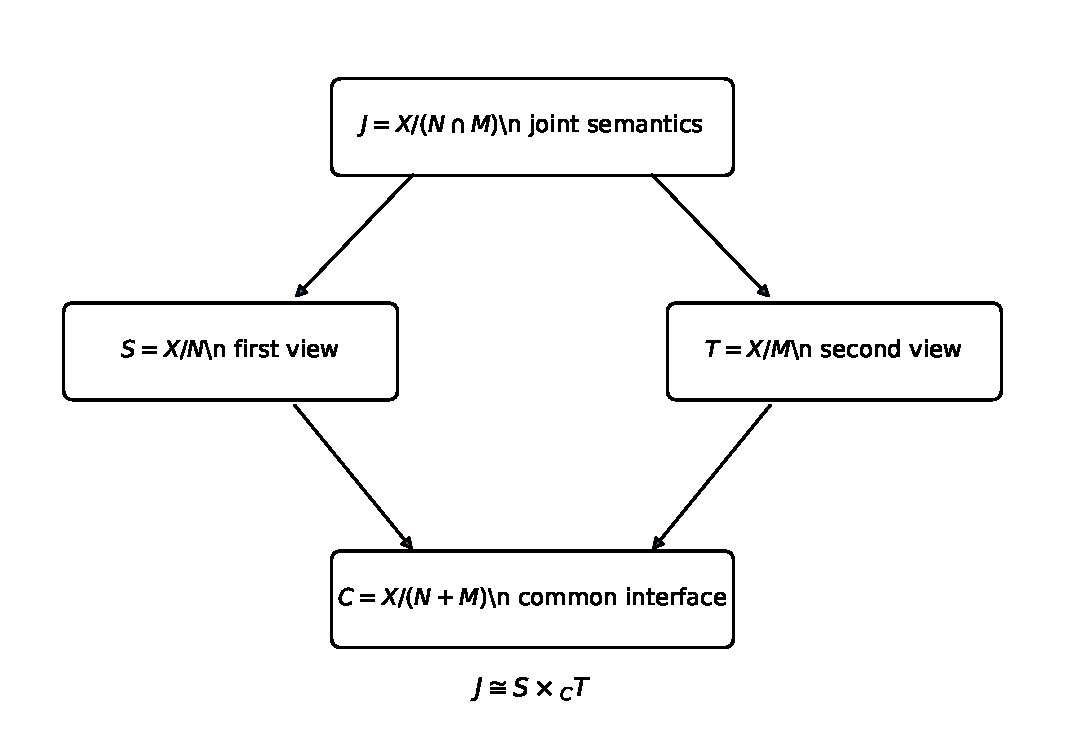
\includegraphics[width=.76\textwidth]{block17_semantic_diamond.pdf}
\caption{The semantic diamond.  The joint representation \(J\) retains both views.  The common quotient \(C\) is the compatibility interface over which the separate coordinates glue.}
\label{fig:block17-semantic-diamond}
\end{figure}

\begin{definition}[Relative semantic residual]
\label{def:block17-relative-residual}
The information needed to augment \(S\) so that it also retains \(T\) is
\[
 R_{T\mid S}
 :=
 \ker(J\to S)
 \cong
 N/(N\cap M)
 \cong
 (N+M)/M.
\]
\end{definition}

\begin{corollary}[Factorization criterion]
\label{cor:block17-factorization-criterion}
The following are equivalent:
\[
 t\text{ factors through }s,
 \qquad
 N\subseteq M,
 \qquad
 R_{T\mid S}=0,
 \qquad
 J\to S\text{ is an isomorphism}.
\]
Moreover,
\[
 0\longrightarrow R_{T\mid S}
 \longrightarrow J
 \longrightarrow S
 \longrightarrow0
\]
is exact.
\end{corollary}

\begin{boundary}[Residuals need not split]
\label{bnd:block17-residual-splitting}
The exact sequence above does not canonically identify \(J\) with \(S\oplus R_{T\mid S}\).  Vector-space extensions split noncanonically.  Module, integral, semiring, filtered, or topological extensions may fail to split.  A residual packet presented as an independent coordinate therefore requires an explicit splitting theorem or constructor passport.
\end{boundary}

\subsection{Exact change of task}
\label{subsec:block17-task-change}

\begin{theorem}[Task-change exact sequence]
\label{thm:block17-task-change}
Let a stronger task have behavioral kernel \(N_s\), and let a weaker task have behavioral kernel \(N_w\), with
\[
 N_s\subseteq N_w.
\]
Then
\[
 0\longrightarrow N_w/N_s
 \longrightarrow X/N_s
 \longrightarrow X/N_w
 \longrightarrow0
\]
is exact.  Thus \(N_w/N_s\) is the exact semantic information discarded when the task is weakened.
\end{theorem}

\begin{proof}
Apply the third isomorphism theorem to the chain \(N_s\subseteq N_w\subseteq X\).
\end{proof}

\begin{corollary}[Composition of task loss]
\label{cor:block17-task-loss-composition}
For
\[
 N_1\subseteq N_2\subseteq N_3,
\]
there is an exact sequence
\[
 0\longrightarrow N_2/N_1
 \longrightarrow N_3/N_1
 \longrightarrow N_3/N_2
 \longrightarrow0.
\]
Hence task loss composes as extension data rather than as a canonically split sum.
\end{corollary}

\begin{resultbox}
\textbf{Semantic quotient result.}
Inside a fixed doctrine, declared future tasks are represented by continuation-stable congruences or subobjects.  Behavioral minimization extracts the maximal stable invisible core.  Task strengthening induces canonical forgetting maps, joint tasks form semantic diamonds, and relative task loss is measured by exact quotient objects.  The construction is relative to the semantic slice and does not define an observer-independent minimum.
\end{resultbox}


\section{Carrier change, observer base change, and provenance}
\label{sec:block18-carrier-observer}

A behavioral quotient is computed inside an observation category, but the represented computation also has a carrier algebra.  Additive convolution, Boolean support, max-plus aggregation, and convex support geometry do not combine routes by the same law.  This section separates carrier translation from observer minimization and gives exact obstruction objects for both.

\subsection{Carrier factorization and joint semantic completion}
\label{subsec:block18-carrier-factorization}

Let \(\mathcal R\) be a raw algebra of expressions or histories for a fixed operation signature.  Let
\[
 s:\mathcal R\longrightarrow S,
 \qquad
 t:\mathcal R\longrightarrow T
\]
be homomorphisms into two semantic carriers.

\begin{theorem}[Carrier factorization gate]
\label{thm:block18-carrier-factorization}
There is a unique homomorphism
\[
 \varphi:\im(s)\longrightarrow T
\]
with \(t=\varphi s\) if and only if
\[
 \kerpair(s)\subseteq\kerpair(t).
\]
When the condition fails, any pair \(x,y\in\mathcal R\) satisfying
\[
 s(x)=s(y),
 \qquad
 t(x)\neq t(y)
\]
is an exact carrier-change obstruction witness.
\end{theorem}

\begin{proof}
Factorization immediately implies constancy of \(t\) on every fiber of \(s\).  Conversely, define
\[
 \varphi(s(x)):=t(x).
\]
The fiber condition makes this well defined.  Since both \(s\) and \(t\) preserve every primitive operation, so does \(\varphi\).  Uniqueness follows because \(s\) is surjective onto its image.
\end{proof}

\begin{definition}[Joint semantic completion]
\label{def:block18-joint-completion}
Define
\[
 j=(s,t):\mathcal R\longrightarrow S\times T,
 \qquad
 J_{s,t}:=\im(j).
\]
The projection
\[
 p_s:J_{s,t}\longrightarrow\im(s)
\]
is the \emph{relative completion map} from the joint semantics to the source semantics.
\end{definition}

\begin{theorem}[Universal joint completion]
\label{thm:block18-universal-joint-completion}
The object \(J_{s,t}\) is the coarsest quotient of \(\mathcal R\) preserving both \(s\) and \(t\).  More precisely, if
\[
 c:\mathcal R\twoheadrightarrow C
\]
admits maps \(a:C\to S\) and \(b:C\to T\) with \(s=ac\) and \(t=bc\), then there is a unique map
\[
 C\longrightarrow J_{s,t}
\]
compatible with both semantics.  Furthermore,
\[
 t\text{ factors through }s
 \quad\Longleftrightarrow\quad
 p_s\text{ is an isomorphism}.
\]
\end{theorem}

\begin{proof}
The pair \((a,b)\) factors \(j\) through \(c\), and the image universal property gives the map to \(J_{s,t}\).  If \(t=\varphi s\), then \(J_{s,t}\) is the graph of \(\varphi\), so \(p_s\) is invertible.  Conversely, if \(p_s\) is invertible, define \(\varphi=p_t p_s^{-1}\).
\end{proof}

\subsection{Behavioral bridges and exact loss}
\label{subsec:block18-bridge-loss}

Let \(f:X\to Y\) be a linear bridge between observational systems, with behavioral kernels \(N_X\subseteq X\) and \(N_Y\subseteq Y\).

\begin{definition}[Task-compatible bridge]
\label{def:block18-task-compatible-bridge}
The bridge is \emph{task compatible} when
\[
 f(N_X)\subseteq N_Y.
\]
Equivalently,
\[
 N_X\subseteq f^{-1}(N_Y).
\]
Then there is a unique induced map
\[
 \overline f:X/N_X\longrightarrow Y/N_Y.
\]
\end{definition}

\begin{theorem}[Bridge-loss exact sequence]
\label{thm:block18-bridge-loss-exact}
For every task-compatible linear bridge, there is an exact sequence
\[
 0\longrightarrow
 \frac{f^{-1}(N_Y)}{N_X}
 \longrightarrow
 \frac{X}{N_X}
 \xrightarrow{\overline f}
 \frac{Y}{N_Y}
 \longrightarrow
 \frac{Y}{N_Y+f(X)}
 \longrightarrow0.
\]
Thus
\[
 L_f:=\frac{f^{-1}(N_Y)}{N_X}
\]
measures source distinctions collapsed by the bridge, while
\[
 E_f:=\frac{Y}{N_Y+f(X)}
\]
measures target semantic states outside the essential image.
\end{theorem}

\begin{proof}
The kernel of \(\overline f\) consists of classes \(x+N_X\) for which \(f(x)\in N_Y\), hence equals \(f^{-1}(N_Y)/N_X\).  The cokernel of \(\overline f\) is the quotient of \(Y/N_Y\) by \((f(X)+N_Y)/N_Y\), which is \(Y/(N_Y+f(X))\).
\end{proof}

\begin{corollary}[Exact semantic equivalence gate]
\label{cor:block18-semantic-equivalence-gate}
The induced bridge \(\overline f\) is an isomorphism exactly when
\[
 L_f=0
 \qquad\text{and}\qquad
 E_f=0.
\]
Faithfulness on the declared task and essential surjectivity on the declared task are therefore independent obligations.
\end{corollary}

\begin{theorem}[Loss-composition extension]
\label{thm:block18-loss-composition}
For induced quotient maps
\[
 Q_X\xrightarrow{\overline f}Q_Y\xrightarrow{\overline g}Q_Z,
\]
there is a natural exact sequence
\[
 0\longrightarrow\ker\overline f
 \longrightarrow\ker(\overline g\,\overline f)
 \longrightarrow\ker\overline g\cap\im\overline f
 \longrightarrow0.
\]
If \(\overline f\) is surjective, this reduces to
\[
 0\longrightarrow L_f
 \longrightarrow L_{gf}
 \longrightarrow L_g
 \longrightarrow0.
\]
\end{theorem}

\begin{proof}
Map \(x\in\ker(\overline g\,\overline f)\) to \(\overline f(x)\).  Its image is exactly \(\ker\overline g\cap\im\overline f\), and its kernel is \(\ker\overline f\).  Surjectivity of \(\overline f\) identifies the intersection with \(\ker\overline g\).
\end{proof}

\begin{boundary}[Loss is extension data]
\label{bnd:block18-loss-extension}
The preceding sequence need not split.  Consequently, composite information loss is not in general a scalar sum or a canonical direct sum of stagewise losses.  A numerical loss budget may be useful, but it is a further invariant of the exact extension rather than a replacement for it.
\end{boundary}

\subsection{Carrier-indexed observer packets}
\label{subsec:block18-carrier-observer-packets}

\begin{theorem}[Carrier-indexed observer packet theorem]
\label{thm:block18-carrier-indexed-observer}
Let \(S\) be a finite continuation-state set, let \((A,\oplus,0)\) be a commutative monoid, let \(B\) be a branch alphabet, and let
\[
 \delta:S\times B\longrightarrow S
\]
be a state transition.  Suppose every branch \(b\in B\) acts by a monoid homomorphism
\[
 L_b:A\longrightarrow A.
\]
For a state packet \(a=(a_s)_{s\in S}\), define
\[
 a'_t
 :=
 \bigoplus_{\delta(s,b)=t}L_b(a_s).
\]
If raw histories have already been aggregated by their state using \(\oplus\), then this update gives exactly the same result as advancing every raw history separately and aggregating afterward.
\end{theorem}

\begin{proof}
Expand the raw history update and group all terms by their predecessor state and new branch.  Associativity and commutativity permit the regrouping.  The identity
\[
 L_b\!\left(\bigoplus_i x_i\right)
 =
 \bigoplus_i L_b(x_i)
\]
then moves aggregation through the branch action.  The displayed formula is the resulting statewise sum.
\end{proof}

Two important realizations have the same state skeleton but different carriers.
\begin{enumerate}
\item For convex value semantics, \(A\) is a family of convex bodies, \(\oplus\) is convex hull of union, and \(L_b(C)=A_b^{\mathsf T}C\).
\item For linear polyphase routing, \(A\) is an additive convolution algebra, \(\oplus\) is coefficient addition, and \(L_b\) multiplies route kernels by the declared filter or transition weight.
\end{enumerate}
The theorem transports the observer skeleton only after the carrier law and the homomorphism obligations are specified.

\subsection{Carrier no-go mechanisms}
\label{subsec:block18-carrier-no-go}

\begin{theorem}[Cancellation barrier]
\label{thm:block18-cancellation-barrier}
Let \(R\) be a nonzero ring and let \(S\) be a nontrivial zerosumfree semiring, so
\[
 a+b=0\Longrightarrow a=b=0.
\]
There is no unital semiring homomorphism \(R\to S\).
\end{theorem}

\begin{proof}
A unital homomorphism \(\varphi\) would give
\[
 0=\varphi(1+(-1))=1_S+\varphi(-1).
\]
Zerosumfreeness forces \(1_S=0\), contradicting nontriviality.
\end{proof}

\begin{theorem}[Idempotence barrier]
\label{thm:block18-idempotence-barrier}
Let \(S\) be a nontrivial unital semiring with idempotent addition, and let \(R\) be an additively cancellative nontrivial semiring.  There is no unital semiring homomorphism \(S\to R\).
\end{theorem}

\begin{proof}
In \(S\), \(1+1=1\).  Its image in \(R\) would satisfy \(1_R+1_R=1_R\), and additive cancellation would imply \(1_R=0\).
\end{proof}

\begin{example}[Haar cancellation]
\label{ex:block18-haar-cancellation}
For the normalized Haar bank,
\[
 \ell=\frac{x_0+x_1}{\sqrt2},
 \qquad
 d=\frac{x_0-x_1}{\sqrt2},
\]
and
\[
 x_0=\frac{\ell+d}{\sqrt2},
 \qquad
 x_1=\frac{\ell-d}{\sqrt2}.
\]
At \(x=(1,0)\), the two route contributions to \(x_0\) are \(1/2,1/2\), while those to \(x_1\) are \(1/2,-1/2\).  Additive reconstruction returns \((1,0)\).  Replacing route addition by maximum returns \((1/2,1/2)\).  The convex/max carrier is therefore not an exact replacement for the signed additive carrier.
\end{example}

\subsection{Observer base change and the relation module}
\label{subsec:block18-observer-base-change}

Let \(E\subseteq K^M\) be the set of distinct residual future functions of a scalar series or observational system.  Set minimization retains the elements of \(E\) as distinct states.  Free linearization produces the vector space \(K^{(E)}\), while linear minimization retains only their span.

\begin{theorem}[Observer base-change exact sequence]
\label{thm:block18-observer-base-change}
The evaluation map
\[
 \pi:K^{(E)}\longrightarrow\Span_K(E),
 \qquad
 \sum_{e\in E}a_e[e]
 \longmapsto
 \sum_{e\in E}a_e e
\]
is surjective and fits into the exact sequence
\[
 0\longrightarrow\Rel_K(E)
 \longrightarrow K^{(E)}
 \xrightarrow{\pi}\Span_K(E)
 \longrightarrow0,
\]
where
\[
 \Rel_K(E):=\ker\pi
\]
is the module of linear relations among distinct discrete residual states.  Hence Set minimization commutes with free linearization exactly when \(E\) is linearly independent.
\end{theorem}

\begin{proof}
Surjectivity is the definition of the linear span.  The sequence is the kernel-cokernel sequence of \(\pi\).  The kernel vanishes exactly when the basis symbols \([e]\) remain linearly independent after evaluation.
\end{proof}

\begin{theorem}[Exact polyphase separation]
\label{thm:block18-polyphase-hankel-separation}
Fix \(N\geq1\) and \(z\neq0\).  Let \(S_z\) be the cyclic shift on \(K^N\) satisfying
\[
 S_z e_j=e_{j+1}\quad(j<N-1),
 \qquad
 S_z e_{N-1}=z e_0,
\]
so \(S_z^N=zI\).  Put
\[
 M_N=I+S_z,
 \qquad
 f_N(n)=e_0^{\mathsf T}M_N^n e_0.
\]
Then the \(N\times N\) Hankel block
\[
 H_{ij}=f_N(i+j),
 \qquad 0\leq i,j<N,
\]
has determinant
\[
 \det H=\pm z^{N-1}.
\]
Consequently its linear residual space has dimension \(N\).  If \(z>0\), the residual functions \(k\mapsto f_N(n+k)\) are pairwise distinct, so the exact discrete future quotient is infinite while the linear continuation dimension is \(N\).
\end{theorem}

\begin{proof}
Factor \(H=OC\), where row \(i\) of \(O\) is \(e_0^{\mathsf T}M_N^i\), and column \(j\) of \(C\) is \(M_N^j e_0\).  For \(j<N\), the binomial expansion of \((I+S_z)^j e_0\) is a unit upper-triangular change from \((e_0,\ldots,e_{N-1})\), hence \(\det C=1\).  The rows \(e_0^{\mathsf T}S_z^k\), \(0\leq k<N\), are \(e_0^{\mathsf T}\) followed by \(z e_{N-k}^{\mathsf T}\), so their determinant is \(\pm z^{N-1}\).  The binomial row change is also unit triangular, proving the determinant formula.

For positive \(z\),
\[
 f_N(n)=\sum_{r=0}^{\lfloor n/N\rfloor}\binom n{Nr}z^r.
\]
The sequence is strictly increasing from index \(N-1\) onward.  Prefixes below \(N\) are distinguished by choosing the first suffix that crosses index \(N\), and later prefixes differ already at suffix zero.  Thus all residual functions are distinct.
\end{proof}

The interpretation of finite Hankel rank as minimal weighted-linear realization dimension is classical weighted-automata theory \cite{CarlylePaz1971,LiRabusseauPrecup2018}.  The displayed family is retained here because it gives an exact internal example of an infinite discrete quotient and a finite linear quotient.

\subsection{Observer-conditioned convex packets}
\label{subsec:block18-convex-provenance}

Let \(S\) be a finite observer-state set and let \(C_s\subseteq\mathbb R^d\) be a compact convex body for each state.  For branch matrices \(A_b\) and transition \(\delta\), put
\[
 C'_t
 =
 \operatorname{conv}
 \bigcup_{\delta(s,b)=t}A_b^{\mathsf T}C_s.
\]

\begin{theorem}[Observer-conditioned convex packet transport]
\label{thm:block18-convex-packet-transport}
For every direction \(x\),
\[
 h_{C'_t}(x)
 =
 \max_{\delta(s,b)=t}h_{C_s}(A_bx).
\]
Repeated updates compose exactly with branch words.  Within each fixed observer state, replacing a finite atom family by any other finite generating family of the same convex hull preserves all future value queries generated by linear branch actions.
\end{theorem}

\begin{proof}
For a linear map \(A\),
\[
 h_{A^{\mathsf T}C}(x)=h_C(Ax).
\]
The support function of the convex hull of a finite union is the maximum of the component support functions.  These two identities give the formula.  Iteration follows from composition of the linear maps and of \(\delta\).  Equality of convex hulls is preserved by linear images and convex hull of union, proving future value equivalence.
\end{proof}

\begin{proposition}[Singular resurrection]
\label{prop:block18-singular-resurrection}
A provenance state carried only by a strictly interior atom may be inactive for every current nonzero linear query and yet become active after an admissible singular continuation.  In particular, if the zero map is admissible, every atom is sent to the same point and all provenance states tie.
\end{proposition}

\begin{proposition}[Invertible hiding]
\label{prop:block18-invertible-hiding}
Assume the total convex body is full-dimensional, query directions are nonzero, and every admissible branch matrix is invertible.  A strictly interior atom remains strictly interior under every continuation and therefore cannot maximize a nonzero linear functional.  Its provenance remains permanently hidden from the declared value query.
\end{proposition}

\begin{proof}
Invertible linear maps preserve relative interior and full dimension.  A nonzero linear functional cannot attain its maximum at a strict interior point of a compact full-dimensional convex body.
\end{proof}

\begin{boundary}[Value, witness, and history are distinct tasks]
\label{bnd:block18-provenance-boundary}
Exact convex geometry determines value semantics and its derived normal-fan structure.  It does not determine branch identity, maximizing multiplicity, or raw history.  Value-only, one-witness, all-witness, and complete-history tasks therefore have different minimal quotients.  No provenance deletion rule is valid without the admissible continuation class and the downstream query family.
\end{boundary}

\begin{resultbox}
\textbf{Carrier and observer result.}
Exact carrier replacement is equivalent to semantic factorization.  When it fails, the joint image is the universal completion preserving both semantics.  Behavioral bridges carry independent kernel-loss and essential-image defects.  Observer minimization then depends on the observation category: discrete residual equality and linear residual span are related by an exact relation module, not by automatic identification.
\end{resultbox}


\section{Admissibility change, geometric obstruction, and doctrine lifting}
\label{sec:block19-admissibility-lifting}

Task strengthening changes which distinctions must be retained.  Enlarging an admissible realization class changes a different quantity: which completions or normal forms are allowed.  The two variances should not be compressed into one undifferentiated order.  This section formalizes admissibility monotonicity, separates gap from nonattainment, and places enrichment problems inside the existing bridge-passport architecture.

\subsection{Admissible realization classes and optimized defect}
\label{subsec:block19-defect}

\begin{definition}[Class-relative defect]
\label{def:block19-class-relative-defect}
Let \(X\) be a represented system, let \(\Gamma\) be a declared class of admissible auxiliary structures, and let
\[
 d(X,g)\in[0,\infty]
\]
be a defect functional.  Define
\[
 \delta_\Gamma(X):=\inf_{g\in\Gamma}d(X,g).
\]
The pair consisting of the infimum and its attainment status is the \emph{class-relative defect profile}.
\end{definition}

\begin{theorem}[Admissibility monotonicity]
\label{thm:block19-admissibility-monotonicity}
If \(\Gamma\subseteq\Gamma'\), then
\[
 \delta_{\Gamma'}(X)\leq\delta_\Gamma(X).
\]
Thus an obstruction in a restricted realization class need not remain an obstruction after the class is enlarged.
\end{theorem}

\begin{proof}
The infimum on the left is taken over a superset of the candidates used on the right.
\end{proof}

\begin{definition}[Completion, gap, and escape]
\label{def:block19-trichotomy}
Assume \(d\geq0\).  The defect profile is:
\begin{enumerate}[label=\textup{(\roman*)}]
\item a \emph{completion} when \(\delta_\Gamma(X)=0\) and the infimum is attained;
\item a \emph{gap obstruction} when \(\delta_\Gamma(X)>0\);
\item an \emph{escape obstruction} when \(\delta_\Gamma(X)=0\) but the infimum is not attained.
\end{enumerate}
\end{definition}

The trichotomy separates approximation from realization.  A sequence of increasingly good coordinates may approach a missing completion only by leaving every compactly controlled part of the admissible parameter space.

\begin{proposition}[Compactness certificate for escape]
\label{prop:block19-escape-compactness}
Let \(\Gamma\) be a Hausdorff parameter space, and let \(d(X,-)\) be continuous.  Suppose every sublevel set satisfying a declared conditioning bound is compact.  If \(\delta_\Gamma(X)=0\) is not attained, then every near-minimizing sequence must eventually violate every such uniform conditioning bound.
\end{proposition}

\begin{proof}
A uniformly conditioned near-minimizing sequence would lie in one compact sublevel set.  A convergent subsequence would have a limit \(g_*\in\Gamma\), and continuity would give \(d(X,g_*)=0\), contradicting nonattainment.
\end{proof}

\subsection{Metric packets and intrinsic distortion}
\label{subsec:block19-metric-distortion}

Let \(T:(V,Q_s)\to(W,Q_t)\) be invertible between finite-dimensional real or complex spaces with positive-definite metrics.  Choose factors \(Q_s=R_s^*R_s\) and \(Q_t=R_t^*R_t\), and put
\[
 B_Q(T):=R_tTR_s^{-1}.
\]
Define
\[
 D_Q(T)
 :=
 \frac{\sigma_{\max}(B_Q(T))}{\sigma_{\min}(B_Q(T))}
 \geq1,
 \qquad
 \Delta_Q(T):=\log D_Q(T).
\]

\begin{proposition}[Coordinate covariance and composition]
\label{prop:block19-distortion-cocycle}
Simultaneous coordinate transport of \(T,Q_s,Q_t\) leaves \(D_Q(T)\) invariant.  For composable invertible maps,
\[
 D_Q(T_2T_1)
 \leq
 D_Q(T_2)D_Q(T_1),
\]
so
\[
 \Delta_Q(T_2T_1)
 \leq
 \Delta_Q(T_2)+\Delta_Q(T_1).
\]
For a closed word \(H\),
\[
 D_Q(H)
 \geq
 \frac{\max_{\lambda\in\operatorname{spec}(H)}|\lambda|}
      {\min_{\lambda\in\operatorname{spec}(H)}|\lambda|}.
\]
\end{proposition}

\begin{proof}
Coordinate transport changes \(B_Q(T)\) by left and right unitary factors.  Singular-value condition numbers are submultiplicative.  The spectral lower bound follows because every eigenvalue modulus lies between the smallest and largest singular values.
\end{proof}

\begin{theorem}[Conformal metric-completion criterion]
\label{thm:block19-metric-completion}
Let a connected finite graph carry invertible edge transports \(T_e\).  Positive-definite vertex metrics and positive edge scales satisfying
\[
 T_e^*Q_{t(e)}T_e=\lambda_e^2Q_{s(e)}
\]
exist if and only if the determinant-normalized holonomy representation preserves a positive-definite metric at one root vertex.  Equivalently, the normalized holonomy is unitarizable.  In finite dimension, this is equivalent to relative compactness of its image.
\end{theorem}

\begin{proof}
A compatible family restricts to an invariant root metric for every normalized closed word.  Conversely, transport an invariant root metric along a spanning tree.  Invariance under fundamental holonomies makes the result path independent, and determinant normalization restores the positive edge scales.  The equivalence between bounded or relatively compact group representations and invariant positive-definite inner products follows by compact-closure averaging.
\end{proof}

\subsection{Exact convex-versus-quadratic separation}
\label{subsec:block19-convex-quadratic}

Consider
\[
 A_1=\begin{pmatrix}1&0\\1&0\end{pmatrix},
 \qquad
 A_2=\begin{pmatrix}0&1\\0&-1\end{pmatrix}.
\]

\begin{theorem}[Sharp geometry-class separation]
\label{thm:block19-convex-quadratic-separation}
The norm \(\|x\|_\infty\) satisfies
\[
 \max\{\|A_1x\|_\infty,\|A_2x\|_\infty\}
 =\|x\|_\infty
\]
for every \(x\in\mathbb R^2\).  In contrast, for every positive-definite quadratic metric \(Q\),
\[
 \max\{\|A_1\|_Q,\|A_2\|_Q\}\geq\sqrt2.
\]
Equality holds for scalar multiples of the Euclidean metric.  Hence the exact optimal convex/Finsler bound is \(1\), while the exact optimal quadratic bound is \(\sqrt2\).
\end{theorem}

\begin{proof}
The two images are
\[
 A_1(x_1,x_2)=(x_1,x_1),
 \qquad
 A_2(x_1,x_2)=(x_2,-x_2),
\]
so the first identity is immediate.

Write
\[
 Q=\begin{pmatrix}a&c\\c&b\end{pmatrix},
 \qquad
 d=ab-c^2>0.
\]
The squared induced norms are
\[
 u:=\|A_1\|_Q^2
 =\frac{b(a+b+2c)}{d},
 \qquad
 v:=\|A_2\|_Q^2
 =\frac{a(a+b-2c)}{d}.
\]
A direct calculation gives
\[
 ab\bigl((a+b)^2-4c^2\bigr)-4(ab-c^2)^2
 =ab(a-b)^2+4c^2(ab-c^2)\geq0.
\]
Thus \(uv\geq4\), and therefore
\[
 \max\{\sqrt u,\sqrt v\}\geq(uv)^{1/4}\geq\sqrt2.
\]
Equality forces \(a=b\) and \(c=0\), and then \(u=v=2\).
\end{proof}

This example is a sharp instance of the established gap between general extremal norms and common quadratic Lyapunov functions \cite{AndoShih1998,John1948}.  Its role here is not a novelty claim.  It proves that obstruction status must record the admissible geometry class.

\subsection{Escape without positive gap}
\label{subsec:block19-unipotent-escape}

\begin{proposition}[Unipotent escape]
\label{prop:block19-unipotent-escape}
Let
\[
 H=\begin{pmatrix}1&1\\0&1\end{pmatrix}.
\]
There is no positive-definite metric \(Q\) with \(H^*QH=Q\).  Nevertheless, for
\[
 Q_s=\operatorname{diag}(s^2,1),
\]
we have
\[
 D_{Q_s}(H)\longrightarrow1
 \qquad(s\downarrow0),
\]
while
\[
 \kappa_2(Q_s)=s^{-2}\longrightarrow\infty.
\]
Thus the metric-completion defect has zero infimum but is not attained.
\end{proposition}

\begin{proof}
Writing \(Q=\begin{psmallmatrix}a&c\\c&b\end{psmallmatrix}\), the equation \(H^*QH=Q\) forces \(a=0\), contradicting positive definiteness.  For \(Q_s\), the metric-normalized matrix is
\[
 \begin{pmatrix}s&0\\0&1\end{pmatrix}
 H
 \begin{pmatrix}s^{-1}&0\\0&1\end{pmatrix}
 =
 \begin{pmatrix}1&s\\0&1\end{pmatrix},
\]
whose singular-value condition number tends to one.  The conditioning formula is immediate.
\end{proof}

\subsection{Forgetful descent and enrichment lifting}
\label{subsec:block19-doctrine-lifting}

Suppose richer categories \(\widetilde{\mathcal C}\) and \(\widetilde{\mathcal D}\) carry forgetful functors
\[
 U:\widetilde{\mathcal C}\to\mathcal C,
 \qquad
 V:\widetilde{\mathcal D}\to\mathcal D.
\]

\begin{proposition}[Forgetful descent and enhancement lifting]
\label{prop:block19-forgetful-lifting}
A rich bridge
\[
 \widetilde B:\widetilde{\mathcal C}\to\widetilde{\mathcal D}
\]
automatically determines an underlying bridge
\[
 V\widetilde B:\widetilde{\mathcal C}\to\mathcal D.
\]
Given only a bare bridge \(B:\mathcal C\to\mathcal D\), constructing \(\widetilde B\) together with a comparison
\[
 V\widetilde B\cong BU
\]
is a lifting problem.  Its existence, uniqueness, and residual automorphisms are additional passport fields and may carry typed obstruction objects.
\end{proposition}

\begin{proof}
The first statement is composition.  The second is not an existence theorem but a precise reformulation of the enhancement problem: a lift is extra structure over the specified commutative square.  Any failure must therefore be recorded relative to the chosen forgetful functors and comparison data.
\end{proof}

The pattern contains several earlier obstruction mechanisms:
\begin{center}
\small
\begin{tabularx}{.96\textwidth}{@{}L{.26\textwidth}L{.28\textwidth}Y@{}}
\toprule
Underlying structure & Requested enrichment & Typed gate or obstruction\\
\midrule
Projective semilinear cocycle & Linear semilinear descent & Relative Brauer class\\
Invertible transport graph & Compatible metric packet & Unitarizability of normalized holonomy\\
Faithful additive realization & Exact tensor fiber functor & Strong monoidal and exactness obligations\\
Max-plus value & Finite-temperature sum semantics & Residual partition mass\\
Bare quotient coordinates & Metric-decorated quotient & Compatible quotient metric and conditioning boundary\\
\bottomrule
\end{tabularx}
\end{center}
No single obstruction object is asserted for all rows.  The common statement concerns the shape of the lifting problem.

\subsection{Two variances and the indexed architecture}
\label{subsec:block19-indexed-architecture}

Task changes and admissibility changes have opposite-looking effects.  If a task is strengthened, its behavioral kernel shrinks and its quotient retains more information:
\[
 N_{\mathrm{strong}}\subseteq N_{\mathrm{weak}},
 \qquad
 Q_{\mathrm{strong}}\twoheadrightarrow Q_{\mathrm{weak}}.
\]
If an admissible realization class is enlarged, the optimized defect can only decrease:
\[
 \Gamma\subseteq\Gamma'
 \quad\Longrightarrow\quad
 \delta_{\Gamma'}\leq\delta_\Gamma.
\]
These are different orders and should not be merged into one scalar notion of a stronger contract.

\begin{definition}[Doctrine-indexed task fiber]
\label{def:block19-task-fiber}
For a doctrine \(D\) and represented object \(X\), let
\[
 \mathsf{Task}_D(X)
\]
denote the ordered family of continuation-stable semantic quotients admitted by the declared query universe.  Inside one fiber, kernel or congruence calculus governs task change.  A change of doctrine
\[
 D\longrightarrow D'
\]
requires a bridge passport specifying carrier transport, preserved constructions, comparison maps, and any lifting obstruction.
\end{definition}

\begin{theorem}[Relative stratified semantic synthesis]
\label{thm:block19-relative-semantic-synthesis}
Within the finite certified setting of this manuscript, the following statements hold.
\begin{enumerate}
\item Every declared semantic slice has a task-relative behavioral quotient whenever the required effective quotient exists.
\item Inside a module-valued slice, joint tasks, common coarsenings, bridge loss, essential-image failure, and task weakening are governed by the exact sequences of \cref{sec:block17-semantic-quotients,sec:block18-carrier-observer}.
\item Carrier changes are legal exactly on the factorization loci certified by \cref{thm:block18-carrier-factorization}; otherwise the joint semantic image is the canonical exact completion preserving both views.
\item Observer changes may introduce additional relation objects such as \(\Rel_K(E)\); they are not inferred from carrier compatibility alone.
\item Enlarging an admissible realization class weakens optimized defect but need not produce an attained completion.
\item Crossing to richer structure is a typed lifting problem and does not follow from the underlying bridge without an enhancement certificate.
\end{enumerate}
\end{theorem}

\begin{proof}
The clauses are respectively \cref{thm:block17-universal-behavioral-coimage,thm:block17-semantic-diamond,thm:block18-bridge-loss-exact,thm:block18-carrier-factorization,thm:block18-observer-base-change,thm:block19-admissibility-monotonicity,prop:block19-forgetful-lifting}.  No clause identifies distinct carriers, observer categories, or admissibility classes without the corresponding comparison data.
\end{proof}

\begin{figure}[htbp]
\centering
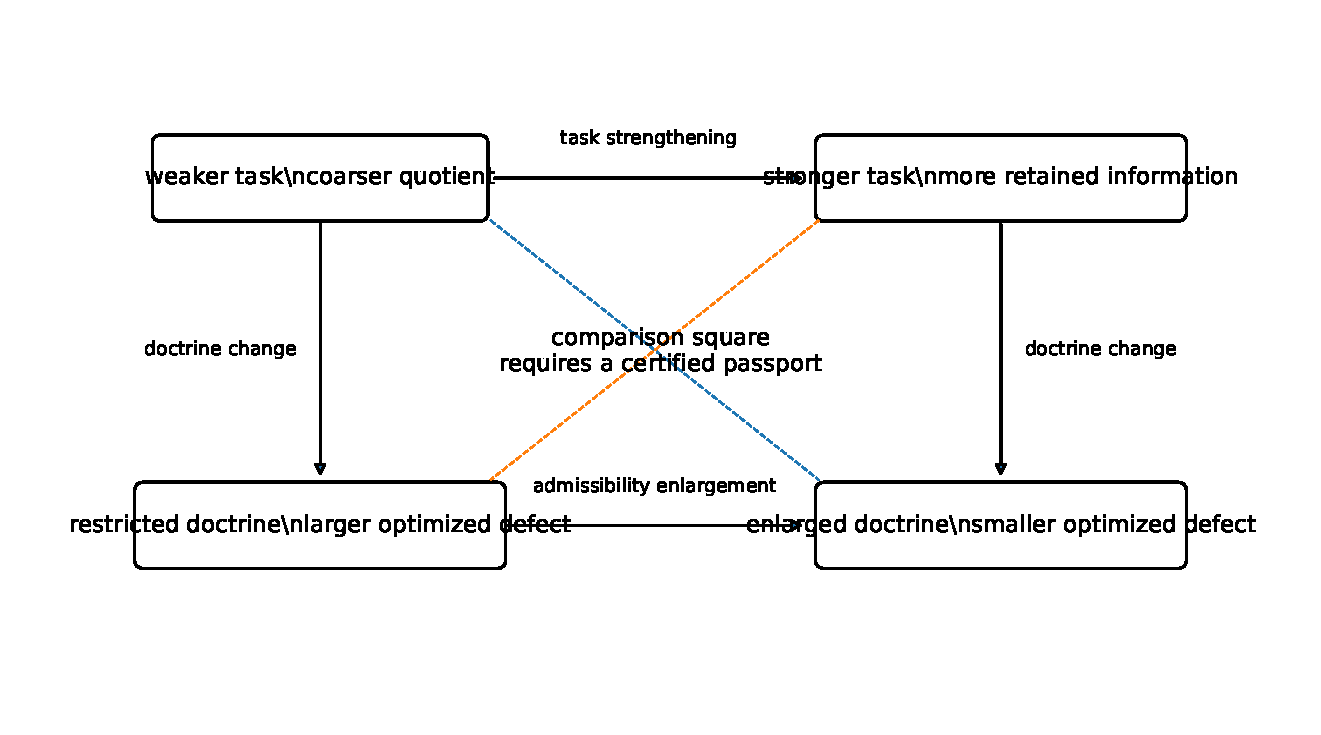
\includegraphics[width=.88\textwidth]{block19_contract_axes.pdf}
\caption{Two independent contract directions.  Horizontal task strengthening retains more semantic information.  Vertical admissibility enlargement allows more realizations and can weaken obstruction.  A commuting square is a theorem-level comparison, not an automatic identification.}
\label{fig:block19-contract-axes}
\end{figure}

\begin{boundary}[Scope of the second-order calculus]
\label{bnd:block19-second-order-scope}
The indexed architecture does not establish a complete double category of all mathematical doctrines, nor does it prove that every task quotient or enrichment is effectively recognizable.  The fiberwise quotient and exact-sequence results are proved in the stated algebraic settings.  Cross-doctrine coherence remains conditional on explicit carrier, topology, metric, tensor, convergence, or higher-categorical passports.
\end{boundary}

\begin{resultbox}
\textbf{Admissibility and lifting result.}
Obstructions are relative to both the requested enrichment and the admissible realization class.  Enlarging that class can remove a positive gap, while zero defect may still fail to be attained.  Rich structure descends under forgetting, but reconstructing it from a bare representation is a lifting problem with its own typed gate.  The resulting architecture is a family of task-quotient fibers connected only by certified doctrine bridges.
\end{resultbox}


\section{Scope, classification targets, and open boundaries}
\label{sec:publication-scope}

The global classification theorem is componentwise because the certified reversible core has five connected semantic components.  The component tag is part of the invariant.  Omitting it would compare objects for which no reversible semantic bridge has been proved.

The lane theorems have a different scope.  The finite profiled Universal Lane Transport Theorem is exact inside a declared additive, idempotent-complete setting with complete split packet systems.  Its realization, kernel, multilinear, fold, and descent clauses apply only under their additional hypotheses.  Trivial address holonomy is required only for one fixed global address set.  With a coherent finite address cocycle, complete matrices instead descend as sections of a matrix local system, and monodromy orbits give the finest ordinary global projector coarsening.  The word ``universal'' refers to this formal lane calculus.  It does not claim that every object has a finite lane presentation or that address count equals dimension, rank, entropy, information, or computational complexity.

The semantic quotient theorem is relative in another direction.  It fixes a carrier doctrine, continuation grammar, observation category, and query family.  The resulting quotient is universal only for that semantic slice.  A different observation category can identify different linear combinations of residual states.  A different carrier can change the legal aggregation law.  A different continuation class can expose provenance that was previously invisible.  There is therefore no observer-independent minimum hidden behind the notation.

The admissibility theory records a third boundary.  A positive defect in a quadratic, integral, finite, or neutral class need not survive enlargement to a convex, rational, completed, or nonneutral class.  Conversely, zero optimized defect does not imply that a completion exists.  Attainment and conditioning remain part of the defect profile.

\begin{landscape}
\begin{table}[htbp]
\centering
\scriptsize
\caption{Certified classification components and exact boundaries.}
\label{tab:block14-scope}
\begin{tabularx}{\linewidth}{@{}L{0.15\linewidth}L{0.23\linewidth}L{0.30\linewidth}Y@{}}
\toprule
Component & Semantic domain & Complete descended coordinates & Boundary \\
\midrule
Digital--regular--linear--Mahler & Fixed-prime regular sequences with rational-mask and periodic subloci & Strict shortlex state, Cartier/mask data where defined, periodic linear data where defined & No all-radix or unrestricted functional/Newton-Mahler equivalence \\
Continuous local & $C(\mathbb Z_p,\mathbb Z_p)$ & Canonical Mahler coefficients and complete clopen branch packets & No universal local-analytic normal form or optimal mixed-radix tree \\
Marked Fuss & $U=z+\alpha U^q$ & Marked parameters $(q,\alpha)$, algebraic branch, recurrence, tree support and orbit data & Complete only on the marked nonlinear--algebraic--holonomic family \\
Euler--multiplicative & Fixed Euler basis and prime-uniform multiplicative locus & Euler exponent, divisor ghost, common local factor, multiplicative function & No arbitrary product-grammar or additive--multiplicative equivalence \\
Finite Galois & One finite semisimple Galois extension & Subgroup, fixed field, Reynolds projector, quotient and Mackey data & No modular/wild or nonneutral tensor reconstruction \\
\bottomrule
\end{tabularx}
\end{table}
\end{landscape}


\subsection{Directional satellites}

Several useful constructions remain adjacent to the reversible core without becoming equivalences:
\begin{itemize}
\item reduction from integral section lattices to finite residue systems, with Smith--Tor ghosts and missing saturated coordinates;
\item passage from a selected algebraic branch to a differential annihilator, which can forget the branch and its minimal polynomial;
\item functional-Mahler masks and Newton--Mahler interpolation, which use different variables and require additional lifting and interpolation data;
\item projective Galois descent, whose lift to an ordinary vector realization is governed by a relative Brauer class;
\item faithful additive or Hilbert-space realizations that do not supply the exact tensor fiber functor required for Tannakian reconstruction;
\item incomplete lane selections and noninjective folds, which retain explicit residuals or collision kernels;
\item Boolean or max-valued summaries of signed additive computation, where cancellation obstructs carrier replacement;
\item Set-valued future quotients and weighted-linear residual spaces, whose difference is measured by a relation module;
\item geometric or provenance compactions that are valid only for the declared continuation class and downstream task.
\end{itemize}
These constructions remain in the directed transformation category with their exact loss, completion, or obstruction records.

\subsection{Open mathematical obligations}

The remaining foundational obligations are more sharply localized than in earlier editions.
\begin{enumerate}
\item Extend the certified atlases across radices, coefficient rings, semirings, and mixed local--global completions without losing normalization or effectivity.
\item Develop modular and wild analogues of finite semisimple Galois projector theory when Reynolds averaging fails.
\item Replace marked model-family results in the holonomic, algebraic, and nonlinear strata by broader native minimality and collision invariants.
\item Construct nonneutral and integral tensor-descent variants with their gerbe or torsor data retained explicitly.
\item Prove finite-data recognition theorems only on declared subgrammars where identifiability and certification are available.
\item Extend finite split and finite holonomy-twisted lane transport to infinite, completed, nonsplit, noninvertible, or genuinely nonadditive resolutions only after specifying the required convergence, exactness, and coherence doctrines.
\item Characterize which query universes are rich enough that every continuation-stable congruence is observationally definable, and determine when the definable task family is closed under joins.
\item Extend the module exact-sequence calculus to exact, regular, homological, enriched, and higher-categorical settings without silently importing additive arguments.
\item Develop effective algorithms for joint semantic completion, relation-module reduction, and task-relative bridge loss beyond finite matrices and finite automata.
\item Construct a fully coherent doctrine-indexed comparison object only after the required horizontal, vertical, and higher comparison cells have been verified.
\end{enumerate}

\begin{boundarybox}
\textbf{No global promotion.}
Completion of the finite atlas, lane theorems, semantic quotient calculus, or class-relative defect theory does not promote absent bridges, incompatible carriers, noninjective folds, unresolved enrichments, or broad-stratum normal forms to equivalences.  Every claimed transport remains relative to its grammar, profile, semantic slice, admissible realization class, and proof-status record.  The detailed obligation and claim ledgers are retained in \cref{app:block14-open-program,app:block14-claim-ledger}.
\end{boundarybox}

\section{Conclusion}
\label{sec:publication-conclusion}

The paper establishes a finite, typed, and auditable form of stratified universality.  Its common object is not one formula and not one global coordinate system.  It is a resolved syntax together with profile-preserving realizations, normalized local charts, typed bridges, task-relative quotients, and declared descent and enrichment doctrines.

The first proof architecture concerns representation.  Packet and refinement data are literal in the additive--Karoubi envelope.  Representation groupoids are separated from information-losing transformations.  Bridge passports identify what is preserved, reflected, forgotten, or only partially defined.  Holonomy, cokernel, Brauer, and higher-coherence defects record different failures of global trivialization.  Effective descent turns compatible local presentations into global semantic objects.  Compatible native invariants descend and become complete on the five declared normalized components.

The finite profiled Universal Lane Transport Theorem isolates the algebraic mechanism inside that architecture.  Complete finite packet systems give exact analysis and synthesis.  Every morphism becomes a unique lane-to-lane block matrix, composition becomes contraction over intermediate addresses, and certified coarsening aggregates fine blocks without changing the underlying morphism.  Selectors split retained transport from named residuals.  The holonomy-twisted extension shows that chart loops may permute lane labels without destroying the calculus.  The matrices then form a local system, descended morphisms are its compatible sections, object-lane orbit sums give the finest ordinary global coarsening, and pair orbits carry exact path composition.

The second proof architecture concerns semantic sufficiency.  For a fixed carrier, continuation grammar, observation category, and query family, the behavioral quotient is the coarsest representation preserving every future observation.  Its kernel is the maximal stable invisible core.  Task strengthening, joint semantics, common coarsening, relative residuals, bridge loss, essential-image failure, and task weakening become exact quotient constructions.  This replaces an informal search for a universally smallest packet by a family of precise minima indexed by declared semantic tasks.

The third architecture concerns changes between those tasks and doctrines.  Carrier replacement is a factorization theorem, not a vocabulary choice.  Observer base change can introduce a relation module even when the carrier is unchanged.  Convex value, additive reconstruction, provenance, and weighted-linear state are therefore distinct semantic objects until a comparison theorem is supplied.  Enlarging an admissible geometry can remove a positive obstruction, while zero infimum can still escape every well-conditioned realization.  Rich structure descends under forgetting, but recovering it from a bare representation is a lifting problem.

The resulting theory is neither storage universality nor a claim that all mathematics is categorically equivalent.  It is a calculus for asking, with explicit types, what survives a change of representation, what is lost, what obstructs reconstruction, what a declared task can safely forget, and what extra structure must be supplied to return.  New strata, task fibers, or doctrines enter the theory only through normalizations, transport laws, effectivity proofs, comparison maps, exact loss records, and claim boundaries.  Historical novelty and independent mathematical review remain separate from this internal formal synthesis.


\appendix

\section{Theorem concordance and proof-status index}
\label{app:full-concordance}

The machine-readable concordance in the source package preserves, for all 75 components, the selected strongest source, exact theorem coordinate, hypotheses, proof class, imported input, and remaining obligation.  The publication PDF retains the compact index below.  This avoids duplicating the full theorem prose while preserving a complete auditable record in \nolinkurl{Komorebi_Theorem_Concordance_v0.4.json} and \nolinkurl{generated/concordance_entries.tex}.

\begin{longtable}{@{}L{0.09\textwidth}L{0.29\textwidth}L{0.22\textwidth}L{0.30\textwidth}@{}}
\caption{Compact index to the theorem concordance. The detailed hypotheses and obligations appear in Appendix~\ref{app:full-concordance}.}\label{tab:compact-concordance}\\
\toprule
ID & Component & Status & Strongest source\\
\midrule
\endfirsthead
\toprule
ID & Component & Status & Strongest source\\
\midrule
\endhead
\midrule
\multicolumn{4}{r}{\small Continued on next page}\\
\endfoot
\bottomrule
\endlastfoot
FND-01 & Typed linear syntax and module semantics & \StatusInternal & \nolinkurl{PSC_I_Symbolic_Core.tex}\\
FND-02 & Finite free seed presentations & \StatusInternal & \nolinkurl{PSC_I_Symbolic_Core.tex}\\
FND-03 & Seed rank and functorial inequalities & \StatusInternal & \nolinkurl{PSC_I_Symbolic_Core.tex}\\
FND-04 & Closed seed-rank formulas & \StatusInternal & \nolinkurl{PSC_I_Symbolic_Core.tex}\\
FND-05 & Exact packet coordinates and reconstruction & \StatusInternal & \nolinkurl{PSC_I_Symbolic_Core.tex}\\
FND-06 & Block algebra and support calculus & \StatusInternal & \nolinkurl{PSC_I_Symbolic_Core.tex}\\
FND-07 & Coordinate transport and transfer naturality & \StatusInternal & \nolinkurl{PSC_I_Symbolic_Core.tex}\\
FND-08 & Subobject, quotient, and packet exactness & \StatusInternal & \nolinkurl{PSC_I_Symbolic_Core.tex}\\
FND-09 & Preservation profiles and theorem transport & \StatusInternal & \nolinkurl{PSC_I_Symbolic_Core.tex}\\
FND-10 & Finite resolved transfer and refinement calculus & \StatusInternal & \nolinkurl{Resolution_Theory_Final_Journal_Manuscript.tex}\\
FND-11 & Universal corner extension and faithful realization & \StatusInternal & \nolinkurl{Resolution_Theory_Final_Journal_Manuscript.tex}\\
FND-12 & Recognition and finite faithful dimension & \StatusInternal & \nolinkurl{Resolution_Theory_Final_Journal_Manuscript.tex}\\
FND-13 & Karoubi, countable, W*, and affiliated completion & \StatusInternal & \nolinkurl{Resolution_Theory_Final_Journal_Manuscript.tex}\\
FND-14 & Nonlinear packet operad and refinement coherence & \StatusInternal & \nolinkurl{Resolution_Theory_Final_Journal_Manuscript.tex; Nonlinear_Transfer_Operad.tex as specialized source}\\
FND-15 & Local analytic nonlinear inversion & \StatusInternal & \nolinkurl{Resolution_Theory_Final_Journal_Manuscript.tex}\\
FND-16 & Universal Lane Transport Theorem, finite profiled form & \StatusInternal & \nolinkurl{block15_section.tex, Universal Lane Transport Theorem and corollaries}\\
FND-17 & Holonomy-Twisted Universal Lane Transport and Orbit Descent & \StatusInternal & \nolinkurl{block16_section.tex, holonomy-twisted transport, orbit descent, orbital composition, and cyclotomic realization}\\
CAT-01 & Representation groupoids separated from directional transformations & \StatusFramework & \nolinkurl{Abstraction_as_a_Resolved_Practice(1).tex; PSC Paper I category of seeded packet systems}\\
GLU-01 & Finite graph holonomy and global-frame criterion & \StatusInternal & \nolinkurl{PSC_Paper_III_Strengthened_Annals_Edition.tex}\\
GLU-02 & Gauge classification of finite transports & \StatusInternal & \nolinkurl{PSC_Paper_III_Strengthened_Annals_Edition.tex}\\
GLU-03 & Maximal path-flat core & \StatusInternal & \nolinkurl{Affine_Mahler_Packets_and_Periodic_Test_Sets.tex (Core-Transfer Addendum 04)}\\
GLU-04 & Split analysis as a genuine two-chart atlas & \StatusInternal & \nolinkurl{Affine_Mahler_Packets_and_Periodic_Test_Sets.tex (Addendum 04)}\\
GLU-05 & Exact affine Mahler chart composition and trivial CRT holonomy & \StatusInternal & \nolinkurl{Affine_Mahler_Packets_and_Periodic_Test_Sets.tex (Addendum 04)}\\
DSC-01 & Descent commutes with complete resolution & \StatusConditional & \nolinkurl{Projector_Calculus_Final_Current.tex}\\
OBS-01 & Canonical obstruction relative to declared correction data & \StatusInternal & \nolinkurl{PSC_Paper_III_Strengthened_Annals_Edition.tex}\\
OBS-02 & Obstruction naturality and packet decomposition & \StatusInternal & \nolinkurl{PSC_Paper_III_Strengthened_Annals_Edition.tex}\\
OBS-03 & Relative/cohomological obstruction & \StatusInternal & \nolinkurl{PSC_Paper_III_Strengthened_Annals_Edition.tex}\\
OBS-04 & Nonlinear correction and complete filtered lifting & \StatusInternal & \nolinkurl{PSC_Paper_III_Strengthened_Annals_Edition.tex}\\
GAL-01 & Finite Galois projector realization & \StatusClassical & \nolinkurl{Resolution_Theory_Galois_Expanded_Journal_Manuscript.tex}\\
GAL-02 & Effective linear semilinear descent & \StatusClassical & \nolinkurl{Resolution_Theory_Galois_Expanded_Journal_Manuscript.tex}\\
GAL-03 & Brauer obstruction to projective descent & \StatusClassical & \nolinkurl{Resolution_Theory_Galois_Expanded_Journal_Manuscript.tex}\\
GAL-04 & Tannakian reconstructed symmetry & \StatusClassical & \nolinkurl{Resolution_Theory_Galois_Expanded_Journal_Manuscript.tex}\\
LIN-01 & C-finite recurrence \(\leftrightarrow\) rational OGF \(\leftrightarrow\) finite state & \StatusClassical & \nolinkurl{Projector_Seed_Calculus_for_Integer_Sequences_Local_Polyphase_Extension.tex}\\
LIN-02 & Minimal linear dimension and similarity normalization & \StatusClassical & \nolinkurl{Projector_Seed_Calculus_for_Integer_Sequences_Local_Polyphase_Extension.tex}\\
LIN-03 & Complete persistent C-finite packet invariant & \StatusInternal & \nolinkurl{Projector_Seed_Calculus_for_Integer_Sequences_Local_Polyphase_Extension.tex}\\
HOL-01 & P-recursive \(\leftrightarrow\) D-finite coefficient translation & \StatusClassical & \nolinkurl{Projector_Seed_Calculus_for_Integer_Sequences_Local_Polyphase_Extension.tex}\\
DIG-01 & Finite digit realization \(\leftrightarrow\) finite k-kernel & \StatusInternal & \nolinkurl{Projector_Seed_Calculus_for_Integer_Sequences_Local_Polyphase_Extension.tex}\\
DIG-02 & Fixed-radix automaton normal form & \StatusClassical & \nolinkurl{Projector_Seed_Calculus_for_Integer_Sequences_Local_Polyphase_Extension.tex}\\
ALG-01 & Selected algebraic branch \(\to\) packet polynomial system & \StatusInternal & \nolinkurl{Projector_Seed_Calculus_for_Integer_Sequences_Local_Polyphase_Extension.tex}\\
TRN-01 & Invertible transform \(\leftrightarrow\) transported packet resolution & \StatusInternal & \nolinkurl{Projector_Seed_Calculus_for_Integer_Sequences_Local_Polyphase_Extension.tex}\\
PRD-01 & Euler-product exponents \(\leftrightarrow\) logarithmic-derivative recurrence & \StatusInternal & \nolinkurl{Projector_Seed_Calculus_for_Integer_Sequences_Local_Polyphase_Extension.tex}\\
MUL-01 & Prime-power seeds reconstruct multiplicative functions & \StatusInternal & \nolinkurl{Projector_Seed_Calculus_for_Integer_Sequences_Local_Polyphase_Extension.tex}\\
LOC-01 & Finite Newton--Mahler reconstruction and local transfer & \StatusInternal & \nolinkurl{Projector_Seed_Calculus_for_Integer_Sequences_Local_Polyphase_Extension.tex}\\
LOC-02 & Exact Mahler \(\leftrightarrow\) affine polyphase coordinate transport & \StatusInternal & \nolinkurl{Projector_Seed_Calculus_for_Integer_Sequences_Local_Polyphase_Extension.tex; Addendum 04 strengthens it}\\
LOC-03 & Sharp minimal integral packet and universal decoder & \StatusInternal & \nolinkurl{Affine_Mahler_Packets_and_Periodic_Test_Sets.tex (Addendum 04)}\\
FMH-01 & Rational functional-Mahler mask \(\to\) Cartier representation & \StatusInternal & \nolinkurl{Komorebi_Custom_GF_Cartier_Padic_Research_Report_0.3.pdf}\\
FMH-02 & Functional-Mahler finite state \(\to\) automaton & \StatusInternal & \nolinkurl{Komorebi_Custom_GF_Cartier_Padic_Research_Report_0.3.pdf}\\
FMH-03 & Finite-mask Cartier transitions \(\leftrightarrow\) carry matrices & \StatusInternal & \nolinkurl{Komorebi_Custom_GF_Cartier_Padic_Research_Report_0.3.pdf}\\
ASM-01 & One explicit profile-indexed resolved envelope & \StatusConjectural & \nolinkurl{Controlling handoff §4 Gap A; local ingredients in Paper I, Resolution Theory, and nonlinear operad sources}\\
ASM-02 & Authoritative declared stratum atlas & \StatusFramework & \nolinkurl{Controlling handoff §4 Gap B}\\
ASM-03 & Bridge semantic, packet, refinement, and residual naturality & \StatusConjectural & \nolinkurl{Controlling handoff §4 Gap C; local naturality inputs FND-07/FND-09/OBS-02}\\
ASM-04 & Triple-overlap and quadruple coherence & \StatusConjectural & \nolinkurl{Controlling handoff §2.6 and §4 Gap C}\\
ASM-05 & Effective descent for the heterogeneous atlas & \StatusConjectural & \nolinkurl{Controlling handoff §4 Gap D}\\
ASM-06 & Native normalization and complete invariants beyond existing slices & \StatusConjectural & \nolinkurl{Controlling handoff §4 Gap E}\\
ASM-07 & Coherent invariant descent and conditional global completeness & \StatusConjectural & \nolinkurl{Controlling handoff §4 Gap F}\\
ASM-08 & Theorem concordance and edition control & \StatusInternal & \nolinkurl{This Work Package 0; Master_Theorem_Migration_Ledger.csv; later migration maps}\\
ASM-09 & Finite Profiled Resolved Atlas Assembly Theorem & \StatusConditional & \nolinkurl{This Work Package 0, §6 and companion LaTeX theorem file}\\
SEM-01 & Universal behavioral coimage and task-relative minimum & \StatusInternal & \nolinkurl{block17_semantic_quotients.tex}\\
SEM-02 & Maximal stable invisible core & \StatusInternal & \nolinkurl{block17_semantic_quotients.tex}\\
SEM-03 & Greatest-fixed-point construction and finite certification & \StatusInternal & \nolinkurl{block17_semantic_quotients.tex}\\
SEM-04 & Task--congruence Galois connection & \StatusInternal & \nolinkurl{block17_semantic_quotients.tex}\\
SEM-05 & Semantic quotient classification by congruences & \StatusClassical & \nolinkurl{block17_semantic_quotients.tex}\\
SEM-06 & Semantic diamond and exact compatibility sequence & \StatusInternal & \nolinkurl{block17_semantic_quotients.tex}\\
SEM-07 & Task-change exact sequence and extension-valued loss & \StatusInternal & \nolinkurl{block17_semantic_quotients.tex}\\
BRG-01 & Task-compatible bridge and five-term exact loss sequence & \StatusInternal & \nolinkurl{block18_carrier_observer_change.tex}\\
BRG-02 & Extension law for composite semantic loss & \StatusInternal & \nolinkurl{block18_carrier_observer_change.tex}\\
CAR-01 & Carrier factorization gate and joint semantic completion & \StatusClassical & \nolinkurl{block18_carrier_observer_change.tex}\\
CAR-02 & Carrier-indexed observer packet theorem & \StatusInternal & \nolinkurl{block18_carrier_observer_change.tex}\\
CAR-03 & Cancellation and idempotence barriers & \StatusClassical & \nolinkurl{block18_carrier_observer_change.tex}\\
OBC-01 & Observer base-change relation module & \StatusInternal & \nolinkurl{block18_carrier_observer_change.tex}\\
OBC-02 & Polyphase infinite-discrete versus finite-linear separation & \StatusInternal & \nolinkurl{block18_carrier_observer_change.tex}\\
CVX-01 & Observer-conditioned convex packet transport and provenance boundary & \StatusInternal & \nolinkurl{block18_carrier_observer_change.tex}\\
ADM-01 & Admissibility monotonicity and completion/gap/escape stratification & \StatusInternal & \nolinkurl{block19_admissibility_lifting.tex}\\
ADM-02 & Sharp convex-versus-quadratic packet separation & \StatusClassical & \nolinkurl{block19_admissibility_lifting.tex}\\
DOC-01 & Forgetful descent, enhancement lifting, and doctrine-indexed task fibers & \StatusFramework & \nolinkurl{block19_admissibility_lifting.tex}\\
\end{longtable}


\clearpage
\section{Edition-control ledger}
\begingroup
\setlength{\tabcolsep}{3pt}
\begin{longtable}{@{}L{0.18\textwidth}L{0.22\textwidth}L{0.25\textwidth}L{0.29\textwidth}@{}}
\caption{Edition-control ledger. Full hashes are retained so later strengthened editions can supersede specific rows without losing provenance.}\label{tab:edition-ledger}\\
\toprule
Source family & Selected file & SHA-256 & Decision\\
\midrule
\endfirsthead
\toprule
Source family & Selected file & SHA-256 & Decision\\
\midrule
\endhead
\midrule
\multicolumn{4}{r}{\small Continued on next page}\\
\endfoot
\bottomrule
\endlastfoot
Paper I canonical symbolic core & \nolinkurl{PSC_I_Symbolic_Core.tex} & \texttt{\seqsplit{39c869f3bd16cbef102fe68dcad51125ab4511077cc45de6d91562c0748fa95c}} & Primary theorem-ID and proof-status spine. Use the Expanded Clarified Edition for exposition, but preserve these stable labels/RecordIDs.\\[3pt]
Paper I expanded clarified edition & \nolinkurl{PSC_Paper_I_Expanded_Clarified_Edition.tex} & \texttt{\seqsplit{e91239446e2e149bbf571c5bbc7e71a76a6f9a351d68963963cfe87f5fbf3c0f}} & Co-primary expository edition, not a replacement for the canonical symbolic RecordID spine.\\[3pt]
Resolution Theory final journal manuscript & \nolinkurl{Resolution_Theory_Final_Journal_Manuscript.tex} & \texttt{\seqsplit{3c0f37a5132c04d0715b0b85a88e34020ffdfc299bf6dd79b7fb4c4bdb32ecec}} & Primary integrated source for finite resolved systems, corner representation/recognition, countable completion, and nonlinear operadic structure.\\[3pt]
Paper III strengthened Annals edition & \nolinkurl{PSC_Paper_III_Strengthened_Annals_Edition.tex} & \texttt{\seqsplit{20452d11443835ca9c0e0484250c01fa51e0456574c7f7c7f5549fbd0f934c89}} & Supersedes older Paper III status language on the relative universal obstruction: coker(D), naturality, quotient projectors, relative exact sequence, and mapping cones are theorem-level. The choice-free cross-problem assignment of D remains open.\\[3pt]
Core-Transfer Addendum 04 & \nolinkurl{Affine_Mahler_Packets_and_Periodic_Test_Sets.tex} & \texttt{\seqsplit{d864bebe02eac16037f17dc677dee9078fbc02a093c7b491b31d2b0208bb91e1}} & Strongest source for maximal directed cores and the exact finite Mahler/polyphase atlas, composite rank law, sharp channel minimum, and stabilization.\\[3pt]
Resolution Theory Galois expanded manuscript & \nolinkurl{Resolution_Theory_Galois_Expanded_Journal_Manuscript.tex} & \texttt{\seqsplit{f3c89f23db5f6e1ee8da7c396c0b30d8274154b8d1fca25d18415ec5dfe54480}} & Primary source for Galois projector strata and classical descent/reconstruction inputs.\\[3pt]
Sequence local/polyphase extension & \nolinkurl{Projector_Seed_Calculus_for_Integer_Sequences_Local_Polyphase_Extension.tex} & \texttt{\seqsplit{e310e5fbec56954e4490615acdeecb04122bad9bd9243e79d84a08174039038a}} & Primary source for the broad sequence grammar, pairwise bridges, persistent C-finite complete packet invariant, and local/polyphase exact transfers.\\[3pt]
Functional-Mahler/Cartier report 0.3 & \nolinkurl{Komorebi_Custom_GF_Cartier_Padic_Research_Report_0.3.pdf} & \texttt{\seqsplit{4480786c49abcb60fb39e07acf0e250c9a3af68c38ac7b4801f34bdaefd5a936}} & Primary source for the rational functional-Mahler \(\to\) Cartier \(\to\) automaton direction and finite-mask Cartier/carry identification.\\[3pt]
Nonlinear transfer operad specialized manuscript & \nolinkurl{Nonlinear_Transfer_Operad.tex} & \texttt{\seqsplit{051970594d8b34c2ec5af67e20e063963b7c8684b75a439f62ed2c5f0e70d3a8}} & Specialized secondary source. Resolution Theory Final is the integrated primary source for overlapping operadic results.\\[3pt]
Abstraction as a Resolved Practice & \nolinkurl{Abstraction_as_a_Resolved_Practice(1).tex} & \texttt{\seqsplit{78bad0bd370fec069f61b5b616dbc5898277229429213a227772a2df4f96861d}} & Conceptual source for representation groupoids, broader directed categories, and atlas language; not the theorem source for heterogeneous effective descent.\\[3pt]
Projector Calculus final current & \nolinkurl{Projector_Calculus_Final_Current.tex} & \texttt{\seqsplit{cc313296416b08ccbe73d893e1744ae840b6419fc5b6676805ef722ab0401b39}} & Selected exact source for descent--limit interchange and cofinal resolution equivalence.\\[3pt]
Master migration ledger & \nolinkurl{Master_Theorem_Migration_Ledger.csv} & \texttt{\seqsplit{dceabf345ac09e507a754a928ca716ed2f797ca9aff8d777e104b49ab73dbdd1}} & Historical dependency/migration evidence only; it does not override a strengthened theorem edition.\\[3pt]
Paper III migration/expansion map & \nolinkurl{MIGRATION_AND_EXPANSION_MAP(1).md} & \texttt{\seqsplit{5f42dc03e5989b8883ce934752c3885ce58ae923b900a02943c86c93e4ca2242}} & Authoritative supersession note for the strengthened Paper III rewrite.\\[3pt]
Remaining open questions after two resolutions & \nolinkurl{Remaining_Open_Questions_and_Conjectures_After_Two_Resolutions.pdf} & \texttt{\seqsplit{13e41d43b9bbeaf0d4e5ed6dd223f6adfaf46c63ebc51987a118d9ec40843c90}} & Historical open-question snapshot. Every ``open'' entry must be checked against later strengthened editions before reuse.\\[3pt]
Universal Lane Transport Theorem, finite profiled form & \nolinkurl{block15_section.tex} & \texttt{\seqsplit{c1ae8aa2472eda9df467bbbf20b3c861f1261333364af06ffaf1cd455b5ab026}} & Selected controlling source for FND-16 and the finite lane-transport theorem family.\\[3pt]
Holonomy-Twisted Universal Lane Transport and Orbit Descent & \nolinkurl{block16_section.tex} & \texttt{\seqsplit{2f4d6deaa95f51b17f4ba107c2b202f28e3b58cca6da516ca3233ed8dd3747ba}} & Selected controlling source for FND-17 and the finite nontrivial-address-holonomy extension.\\[3pt]
Part IV semantic quotient calculus & \nolinkurl{block17_semantic_quotients.tex} & \texttt{\seqsplit{d8355db51d374b93114e9f2f00de7f6bf529eee89939573e3da51fecea981bc6}} & Primary source for behavioral cores, task congruences, semantic diamonds, residuals, and task-change exactness.\\[3pt]
Part IV carrier and observer calculus & \nolinkurl{block18_carrier_observer_change.tex} & \texttt{\seqsplit{9307836727c1bfdb7159d883529812c920dd9517c6042a72383876e45aaebbd0}} & Primary source for carrier factorization, joint completion, bridge loss, observer base change, and provenance.\\[3pt]
Part IV admissibility and lifting calculus & \nolinkurl{block19_admissibility_lifting.tex} & \texttt{\seqsplit{9368eeae300343c809895304e35c454514b32b4369e03354ad00317b6da5f1dc}} & Primary source for optimized defect, completion/gap/escape, geometry-class separation, and enrichment lifting.\\[3pt]
Part IV exact symbolic validation & \nolinkurl{results/block17_semantic_extension_validation.json} & \texttt{\seqsplit{218123b49533a702126e8eea6f2e5f5172d4e9802902c6acb2460d39c0d334d1}} & Finite exact implementation audit retained separately from universal proofs.\\[3pt]
\end{longtable}
\endgroup


\clearpage
\section{Publication audit and development provenance}
\label{app:block15-publication-audit}

The consolidated edition retains a compact theorem-suite map and a development-provenance ledger so that editorial reordering does not erase proof dependencies or claim boundaries.

\begin{table}[htbp]
\centering
\small
\caption{Publication-source audit for the Finite lane-transport theorem consolidated edition.}
\label{tab:block15-publication-audit}
\begin{tabularx}{\textwidth}{@{}L{0.27\textwidth}YL{0.12\textwidth}@{}}
\toprule
Audit area & Record & Status \\
\midrule
Source graph & 55 TeX files & PASS \\
Abstract length & 316 words & PASS \\
Labels and references & 519 labels; 131 references & PASS \\
Citation keys & 14 cited keys & PASS \\
Graphics & 57 included assets & PASS \\
Lane verifier & 197,099 exact assertions & PASS \\
Publication structure audit & 77 assertions & PASS \\
\bottomrule
\end{tabularx}
\end{table}


\IfFileExists{generated/block16_publication_audit_table.tex}{\begin{table}[htbp]
\centering
\small
\caption{Publication-source and release-integrity audit for the Block 16 holonomy-twisted extension.}
\label{tab:block16-publication-audit}
\begin{tabularx}{\textwidth}{@{}L{0.27\textwidth}YL{0.12\textwidth}@{}}
\toprule
Audit area & Record & Status \\
\midrule
Source graph & 60 TeX files & PASS \\
Abstract & 346 words & PASS \\
Labels and references & 542 labels; 138 references & PASS \\
Citation keys & 14 cited keys & PASS \\
Graphics & 57 included assets & PASS \\
Block 16 verifier & 1,344,823 exact assertions & PASS \\
Concordance & 57 synchronized entries through FND-17 & PASS \\
Compiled PDF & 239 pages & PASS \\
Publication audit & 85 checks & PASS \\
\bottomrule
\end{tabularx}
\end{table}
}{}

\begin{table}[htbp]
\centering
\small
\caption{Final formal-foundations publication audit.}
\label{tab:formal-foundations-v2-audit}
\begin{tabularx}{\textwidth}{@{}L{0.31\textwidth}Y@{}}
\toprule
Audit surface & Recorded result\\
\midrule
Source graph & 65 recursively included TeX files; 620 labels; 153 source references\\
Concordance & 75 components with synchronized status and domain counts\\
Inherited validation & Block 15 PASS; Block 16 PASS with 1,344,823 assertions\\
Part IV validation & 3,022 exact symbolic assertions; zero recorded failures\\
Compiled artifact & 247 pages; metadata, theorem-layer text, references, citations, and graphics checked\\
Audit result & 77 checks; 0 failures\\
Boundary & Internal publication integrity only; not independent peer review or historical-priority validation.\\
\bottomrule
\end{tabularx}
\end{table}


\begin{longtable}{@{}L{0.27\textwidth}L{0.65\textwidth}@{}}
\caption{Development provenance retained after journal-facing reorganization.}\label{tab:block14-development-ledger}\\
\toprule
Stage & Mathematical contribution \\
\midrule
\endfirsthead
\toprule
Stage & Mathematical contribution \\
\midrule
\endhead
Foundation & Typed resolved syntax, packet coordinates, preservation profiles, additive-Karoubi envelope \\
Atlas typing & Normalized strata, representation groupoids, bridge passports, information loss, obstruction types \\
Finite effectivity & Periodic and rational-mask heterogeneous atlases \\
Digital normalization & Fixed-radix regular, automatic finite-orbit, and integral prime-power layers \\
Product/local normalization & Euler--multiplicative and Newton-Mahler--polyphase atlases \\
Holonomic, algebraic, nonlinear & Marked model-family minimality, collision, and tree signatures \\
Symmetry & Finite Galois, Brauer, profinite, and neutral Tannakian slices \\
Global synthesis & Authoritative bridge matrix, higher coherence, invariant descent, tagged completeness \\
Lane transport & Complete finite-resolution analysis, synthesis, block transport, refinement, selection, residual accounting, and typed specializations \\
Holonomy transport & Matrix local systems, exact twisted synthesis, base-fiber invariants, monodromy-orbit coarsening, and orbital composition \\
Publication consolidation & Theorem spine, proof-order reorganization, scope compression, and source audit \\
\bottomrule
\end{longtable}


\clearpage
\section{Detailed open-obligation ledger}
\label{app:block14-open-program}

\subsection{Correct dependency order}

The remaining heterogeneous work has a strict topological order:
\[
\boxed{
\begin{gathered}
\text{profiled envelope}
\longrightarrow
\text{declared atlas}
\longrightarrow
\text{typed bridge laws}\\[-1pt]
\longrightarrow
\text{higher coherence}
\longrightarrow
\text{effective descent}
\longrightarrow
\text{compatible invariants}
\end{gathered}}
\]
The first three arrows cannot be skipped. Pairwise formulas do not themselves define a pseudofunctor. Local completeness does not itself construct compatible global isomorphisms.

\subsection{What this manuscript closes}

This paper closes the following finite parts of the program:

\begin{itemize}
\item the typed finite resolved signature, exact finite packet/refinement/residual calculus, preservation-profile gate, and additive split-idempotent resolved envelope;
\item the formal finite atlas assembly theorem;
\item explicit profiled stratum passports, normalized subcategories, representation groupoids, and the typed directed transformation category;
\item bridge passports, bridge classes, information-loss profiles, overlap categories, bridge-law certificates, and a concrete higher-coherence defect;
\item the split-bridge reversible-core theorem, the maximal holonomy-fixed path-flat core, and the exact obstruction-rank formula;
\item the relative cokernel, coarsening exact sequence, mapping-cone extension, Hilbert-90 effectivity, Brauer obstruction, and Tannakian boundary in one typed comparison;
\item a precise isomorphism-effectivity condition for global invariant completeness;
\item two exact finite affine-Mahler atlas models;
\item the normalized C-finite recurrence-rational-state atlas with effective object and morphism descent;
\item cross-presentation descent of the exact C-finite packet-complexity profile;
\item a four-chart atlas spanning linear, digital, and functional-Mahler strata on the unit purely periodic domain;
\item complete bridge passports for that atlas, including the directional Cartier compiler lane and its exact loss profile;
\item all four triple-overlap laws, the quadruple coherence equation, effective object and morphism descent, and a globally complete compatible invariant package;
\item the Frobenius-radical characterization of rational canonical masks and the exact divisor-residue obstruction to rational collapse;
\item the canonical finite Cartier module, its reachable-observable minimality theorem, and the exact identification of reachable compiler states with the \(p\)-kernel;
\item effective descent across reduced mask, minimal Cartier-module, and minimal DFAO charts on the full unit rational-mask domain;
\item a globally complete rational-mask invariant package and a strict negative control showing that the rational-mask atlas is a proper subatlas of the automatic stratum;
\item the canonical section-module, strict shortlex, minimal digit-linear, and word-Hankel normalization theorem for every fixed-radix field-valued regular sequence;
\item the automatic finite-orbit theorem over finite fields, including exact state-to-rank bounds and a strict compression corpus;
\item the canonical raw and saturated integral section lattices for every integer-valued sequence of finite rational section rank;
\item the digit-equivariant Smith--Tor reduction sequence, exact Smith and Fitting formulas, and good-prime criterion;
\item finite minimal prime-power semantic section automata with explicit ambient module bounds and compatible reduction maps;
\item the \(p\)-adic and profinite completion sequences, disappearance of finite ghost coordinates, persistence of the missing saturation quotient, and the separate integral and actual-section effectivity obstructions;
\item the integral fixed-Euler-basis classification, divisor-ghost integrality locus, exact logarithmic-derivative recurrence, and finite-prefix triangular normalization;
\item prime-power effective descent for integral multiplicative arithmetic functions, complete local Euler and ghost coordinates, valuation logarithmic derivatives, and multiplicative residue packets;
\item the restricted divisor--ghost product--multiplicative atlas with effective object and morphism descent and a complete prime-power invariant;
\item the continuous Newton--Mahler coefficient theorem as a normalized local chart, complete clopen branch analysis and synthesis, and strict nested branch coherence;
\item exact affine Mahler coefficient transport, mixed-radix kernel composition, Chinese-remainder diamonds, and the complete branch-coefficient packet equivalence;
\item the finite-degree bridge ladder, sharp integral and fixed-modulus packet sizes, explicit integer decoders, and prime-power rank-loss formulas;
\item branchwise valuation ledgers, Frobenius sparsification, matrix Carmichael--Mahler state constructors, and principal-unit precision amplification;
\item canonical monic minimal differential and tail-recurrence Ore charts, together with the finite transient ledger needed for exact reconstruction;
\item the general arithmetic-multisection defect decomposition into orbit aliasing and address cancellation, with singularity-orbit and local-exponent passports;
\item the exact hypergeometric packet equation, minimal differential-order phase diagram, orbit rank, and complete marked invariant for the binomial--Fuchsian model family;
\item finite selected-branch algebraic normalization, exact residue-packet polynomial systems, the generic $d^N$ packet-degree theorem, and explicit tuple/stabilizer collision signatures;
\item the marked polynomial fixed-point atlas across complete packet jets, colored operation trees, and exact packet equations;
\item exact repeated-direction packet Fa\`a di Bruno compression by colored integer-partition profiles;
\item exact SCC elimination to the address-preserving cyclic nonlinear core;
\item the finite arity-gcd tree signature controlling arithmetic packet support and the complete dominant-singularity orbit, together with the full $q$-ary phase theorem;
\item the normalized finite subgroup--fixed-field--Reynolds atlas, exact normality and quotient-compression criterion, conjugate nonnormal atlas envelopes, and Mackey double-coset transition packets;
\item nested ramification projectors and the weighted unresolved-rank formulas for Artin and Swan conductors;
\item effective finite Galois vector descent, the framed Hilbert-90 chart, the exact relative Brauer obstruction, profinite finite-level reconstruction, and the neutral Tannakian tensor-fiber gate;
\item an authoritative bridge matrix with named restricted equivalence loci, directional-loss entries, partial constructors, and explicit absent bridges;
\item normalizer-induced triple and quadruple coherence for every reversible cycle in the certified finite atlas;
\item coherent invariant comparison maps and effective invariant descent on five connected components;
\item a complete tagged global invariant on the digital--regular--functional-Mahler, continuous Newton--Mahler, marked Fuss, Euler--multiplicative, and finite Galois semantic union;
\item the weighted Fuss--Catalan nonlinear--algebraic--holonomic equivalence and its complete finite parameter invariant.
\item the finite profiled Universal Lane Transport Theorem: exact analysis and synthesis, unique transfer blocks, compositional contraction, compatible coarsening, selectors and residuals, profiled realizations, conditional kernel and fold-loss clauses, factorial residue realization, and overlap-compatible descent under an explicit address cocycle.
\item the finite holonomy-twisted lane extension: matrix-local-system analysis and synthesis, twisted path contraction, equivariant resolution change, holonomy-compatible selectors and residuals, the finest monodromy-orbit projector coarsening, pair-orbit transport atoms, orbital structure constants, and rational cyclic Fourier-orbit descent.
\end{itemize}

\subsection{What remains}

\begin{longtable}{@{}L{0.07\textwidth}L{0.20\textwidth}L{0.17\textwidth}L{0.48\textwidth}@{}}
\caption{General extension obligations after the formal foundations v2.0 milestone.}\label{tab:proof-obligations}\\
\toprule
ID & Obligation & Current status & Remaining completion criterion\\
\midrule
\endfirsthead
\toprule
ID & Obligation & Current status & Remaining completion criterion\\
\midrule
\endhead
\midrule
\multicolumn{4}{r}{\small Continued on next page}\\
\endfoot
\bottomrule
\endlastfoot
PO-01 & Extend the profile-indexed resolved envelope & \StatusConditional & The additive-Karoubi core is proved. Add nonlinear, completion, monoidal, or integral doctrines only for newly selected strata and prove the corresponding profile-indexed universal property.\\[3pt]
PO-02 & Freeze explicit finite atlases & \StatusInternal & Closed for the unit-periodic, rational-mask, fixed-radix regular, product-multiplicative, continuous local Newton--Mahler, marked binomial--Fuchsian, selected algebraic, marked nonlinear-tree, and finite semisimple Galois atlases, and assembled into the five-component certified Block 13 atlas. Every further enlargement must again declare its semantic domain, chart categories, overlap categories, and component tag.\\[3pt]
PO-03 & Define morphisms and normalized subcategories & \StatusInternal & Closed for fixed-radix regular sequences, the canonical integral raw/saturated lattice record, fixed-basis Euler products, integral multiplicative functions, and continuous Newton--Mahler functions with complete branch packets. The marked binomial--Fuchsian holonomic chart, selected one-variable algebraic branch chart, marked polynomial fixed-point chart, finite semisimple subgroup chart, framed semilinear vector chart, and neutral Tannakian chart are closed; unrestricted holonomic, multivariate algebraic, unmarked nonlinear, semiring, cross-radix, unrestricted-product, modular, wild, and nonneutral enlargements remain separate passport obligations.\\[3pt]
PO-04 & Type each bridge & \StatusInternal & Closed for the authoritative Block 13 matrix on the certified domains, including equivalences on named overlaps, fully faithful inclusions, directional losses, constructors, partial bridges, and explicit absent cells. Every extension must retain the same bridge passport and information-loss discipline.\\[3pt]
PO-05 & Prove bridge naturality & \StatusInternal & Closed for digit sections, behavior quotients, Hankel factorization, Smith reduction, Euler logarithmic derivatives, local Dirichlet products, divisor-ghost inversion, Mahler analysis and synthesis, affine polyphase transport, mixed-radix composition, valuation certificates, coefficient/Ore translation, hypergeometric packet synthesis, the marked alias/cancellation ledger, packet-polynomial residue reduction, Weil-restriction degree transport, the algebraic collision ledger, diagonal packet Faà di Bruno profile compression, SCC elimination, marked tree-address transport, subgroup inclusion, Reynolds averaging, normal quotient compression, Hilbert-90 gauge trivialization, and projective Brauer boundary transport on the declared overlaps.\\[3pt]
PO-06 & Prove higher coherence & \StatusInternal & Closed on every reversible cycle of the five-component certified atlas by the Block 13 normalizer-induced coherence theorem. Unframed vector descent retains intrinsic GL automorphisms, and broader atlases may have nontrivial comparison automorphisms or nonvanishing higher defects.\\[3pt]
PO-07 & Prove object effectivity & \StatusInternal & Closed for the verified digital, regular, integral, fixed-Euler-basis, multiplicative, divisor-ghost, and continuous Newton--Mahler domains, the marked binomial--Fuchsian domain, the selected algebraic branch domain, the marked nonlinear-system domain, the finite subgroup/projector domain, and framed finite Galois vector descent by explicit normalization from the represented semantic object and retained generator or symmetry data.\\[3pt]
PO-08 & Prove morphism effectivity & \StatusInternal & Closed for the verified atlases because their normalized fibers are contractible or discrete; the complete clopen local packet also glues equality morphisms by explicit piecewise synthesis; the marked holonomic, selected algebraic, and marked nonlinear fibers are discrete; finite Galois vector morphisms descend by fixed points and scalar extension. Unframed symmetry groupoids retain intrinsic automorphisms and require genuine groupoid descent.\\[3pt]
PO-09 & Construct native comparison maps & \StatusInternal & Closed on the five certified components. Block 13 packages the digital-regular-mask-periodic, continuous Newton--Mahler, marked Fuss, Euler--multiplicative, and finite Galois native coordinates into coherent comparison families. Comparisons for unrestricted broad strata remain separate obligations.\\[3pt]
PO-10 & Control isomorphism descent & \StatusInternal & Closed for the five-component certified atlas: normalized fibers are discrete or contractible, comparison cells are coherent, and compatible local isomorphisms descend. In broader atlases identify or kill holonomy, cokernel, Brauer, nonneutral tensor, or higher-coherence obstructions.\\[3pt]
PO-11 & Broaden automatic and regular invariants & \StatusConditional & Fixed-radix field normalization, canonical integral saturation, Smith--Fitting reduction profiles, and compatible prime-power semantic towers are closed under the Block 06 hypotheses. Cross-radix comparison, arbitrary coefficient rings and semirings, and effective recognition from finite data remain open.\\[3pt]
PO-12 & Normalize product and multiplicative strata & \StatusInternal & Closed for the fixed integral Euler basis, integral multiplicative functions, and the multiplicative divisor-ghost overlap. Minimal compilers, unrestricted product grammars, monoidal closure of the overlap, and any global Cauchy-Dirichlet equivalence remain open.\\[3pt]
PO-13 & Broaden local Mahler theory & \StatusInternal & Closed for continuous \(\mathbb Z_p\)-valued functions, canonical Newton--Mahler coefficients, complete clopen and coefficient packets, finite-degree affine channels, sharp standard packet sizes, and principal-unit precision ladders. Exact higher kernel valuations, optimal mixed-radix trees, nonlinear local systems, state recognition, and a combined spectral--local signature remain open.\\[3pt]
PO-14 & Broaden holonomic packet minimality & \StatusConditional & Canonical minimal Ore charts and the marked binomial--Fuchsian packet-order theorem are closed. General minimal multisection operators, canonical desingularization, monodromy-extension data, differential-module cyclicity, and a finite signature beyond the marked family remain open.\\[3pt]
PO-15 & Broaden algebraic packet minimality & \StatusInternal & Finite selected-branch normalization, exact packet polynomial systems, the generic \(d^N\) Weil-restriction bound, and marked collision signatures are closed. Minimal multivariate system dimension, optimal symmetry-reduced degree bounds, ramified Puiseux passports, and universal branch-recognition algorithms remain open.\\[3pt]
PO-16 & Broaden nonlinear and tree signatures & \StatusInternal & Closed for marked polynomial fixed points, complete packet jets, repeated-direction Faà di Bruno profile compression, address-preserving SCC reduction, and positive simply generated tree support and dominant-orbit signatures. Arbitrary mixed directions, coordinate-free minimum nonlinear system dimension, sign-canceling tree weights, unmarked generators, noncontractive global dynamics, and a universal operadic normal form remain open.\\[3pt]
PO-17 & Extend modular, wild, and nonneutral symmetry & \StatusConditional & Finite semisimple Reynolds charts, framed Hilbert-90 descent, the projective Brauer obstruction, profinite finite-level reconstruction, and neutral Tannakian symmetry are closed. Derived fixed points, integral wild ramification, group-scheme torsion, nonneutral fiber functors, and gerbe-valued descent remain open.\\[3pt]
PO-18 & Maintain theorem and edition provenance & \StatusConditional & Ongoing. Every new claim must cite the selected strongest edition, exact theorem, hypotheses, imported input, and superseded predecessor.\\[3pt]
PO-19 & Separate internal proof from external validation & \StatusConditional & Ongoing. Keep direct proof, exact computation, imported classical theorem, conjecture, and independent peer review in distinct status fields.\\[3pt]
PO-20 & Extend the global invariant beyond the certified spine & \StatusConditional & Work Package 6 is closed on the five-component finite atlas. Remaining targets are cross-radix comparison, semiring and all-ring normalization, unrestricted holonomic and multivariate algebraic invariants, unmarked nonlinear systems, modular and wild symmetry, nonneutral tensor descent, and any genuine bridges joining the current component tags.\\[3pt]
PO-21 & Extend lane transport beyond the finite profiled theorem & \StatusConditional & The complete finite split-idempotent calculus and its finite nontrivial-address-holonomy extension are closed under their printed hypotheses. Complete matrices descend as matrix-local-system sections, monodromy orbits give the finest ordinary projector coarsening, and pair orbits govern compatible selectors. Infinite resolutions, non-split decompositions, noninvertible transitions, general nonlinear doctrines, higher-stack effectivity, historical novelty, and unrestricted atlas globalization remain separate obligations.\\[3pt]
PO-22 & Recognize task quotients effectively & \StatusConditional & The fiberwise behavioral quotient and finite-dimensional stabilization theorems are proved. Effective recognition for infinite systems, symbolic query languages, enriched observations, and undecidable continuation grammars remains open.\\[3pt]
PO-23 & Extend exact semantic loss beyond modules & \StatusConditional & The semantic diamond, bridge-loss sequence, and extension law are proved in module categories. Exact, regular, homological, semiring, topological, and higher-categorical analogues require their own quotient and exactness doctrines.\\[3pt]
PO-24 & Classify carrier and observer comparison maps & \StatusConditional & Kernel factorization and the joint semantic completion are closed for algebraic carriers, and the relation module is closed over fields. Classification of lawful changes among noncommutative, measure-valued, completed, probabilistic, and nonlinear carriers remains open.\\[3pt]
PO-25 & Control admissibility and attainment & \StatusConditional & Admissibility monotonicity and the completion/gap/escape trichotomy are proved. Effective optimal-geometry construction, attainment criteria, and conditioning rates remain doctrine-specific.\\[3pt]
PO-26 & Build doctrine-level coherence only from certified cells & \StatusFramework & The doctrine-indexed task-fiber architecture is stated and several concrete lifting gates are proved. A complete double category, bicategory, or higher stack of doctrines is not yet constructed and must not be inferred from the fiberwise theorems.\\[3pt]
\end{longtable}


\subsection{Finite completion criterion}

A rigorous first heterogeneous stratified-universality theorem should be declared complete only after the following finite milestone is met:

\begin{enumerate}
\item a profile-indexed envelope is constructed for every profile used by the selected atlas;
\item at least two genuinely different normalized strata are fully specified as categories;
\item every overlap bridge is typed and its information loss is stated;
\item every nonempty triple-overlap coherence equation is proved;
\item descent for objects and morphisms is effective;
\item one nontrivial native invariant family has coherent comparison maps and a proved global completeness theorem on the normalized descent category;
\item the theorem concordance and source-edition ledger are synchronized with the final manuscript.
\end{enumerate}

The C-finite theorem completes a three-chart presentation atlas within one stratum.  \Cref{thm:first-heterogeneous-descent,thm:periodic-invariant-completeness} meet all seven items for a restricted atlas spanning three strata.  \Cref{thm:rational-mask-effective-descent,thm:rational-mask-invariant-descent} enlarge the digital and functional-Mahler overlap from unit pure periodicity to every unit series with rational canonical mask.  \Cref{thm:block05-regular-rank,thm:block05-shortlex-normal-form,thm:block05-regular-atlas} close fixed-base field-valued regular normalization.  \Cref{thm:block06-saturation,thm:block06-tor-sequence,thm:block06-integral-normalization} close the canonical integral saturation and prime-power reduction package for integer-valued sequences already known to have finite rational section rank.  \Cref{thm:block07-euler-classification,thm:block07-prime-power-descent,thm:block07-product-multiplicative-descent,thm:block07-complete-product-invariant} now close fixed-basis product normalization, multiplicative prime-power normalization, and one explicit cross-stratum invariant overlap.  \Cref{thm:block08-mahler-coordinate,thm:block08-clopen-equivalence,thm:block08-kernel-composition,thm:block08-sharp-packet,thm:block08-precision-amplification} now close the continuous Newton--Mahler chart, complete local polyphase descent, finite-degree collective recovery, and the principal-unit precision ladder.  \Cref{thm:block09-ordinary-atlas,thm:block09-multisection-closure,thm:block09-general-defect-identity,thm:block09-order-phase,thm:block09-marked-descent} now close canonical Ore normalization, the general two-stage multisection defect ledger, and one exact marked regular-singular model case.  \Cref{thm:block10-branch-atlas,thm:block10-exact-packet-system,thm:block10-packet-degree-bound} closes the selected one-variable algebraic chart.  \Cref{thm:block11-marked-atlas,thm:block11-compressed-faa,thm:block11-scc-reduction,thm:block11-tree-address,thm:block11-dominant-orbit,thm:block11-qary-phase} now close the marked polynomial-system atlas, diagonal composition compression, address-preserving cyclic-core reduction, and one finite tree-signature family.  \Cref{thm:block12-normalized-galois-chart,thm:block12-vector-descent,thm:block12-brauer,thm:block12-galois-assembly} close the finite semisimple subgroup atlas, effective linear semilinear descent, exact projective obstruction, and the neutral tensor reconstruction gate.  \Cref{thm:block13-normalizer-coherence,thm:block13-certified-invariant-descent,thm:block13-fuss-equivalence,thm:block13-global-completeness} now complete the finite global-invariant milestone: five certified connected components, coherent comparison maps, effective componentwise descent, and a complete tagged invariant on the declared semantic coproduct.  The remaining program is therefore a cross-radix, semiring, modular and wild symmetry, nonneutral tensor, unrestricted holonomic, multivariate algebraic, general nonlinear, stronger local-valuation, optimal mixed-radix, and unrestricted product-grammar compatibility problem rather than a missing elementary Mahler-coordinate, Ore-normalization, rooted-tree expansion, finite Galois descent, or finite certified invariant-descent theorem.

Block 15 closes the common complete finite-resolution lane calculus under its printed hypotheses. Block 16 removes trivial address holonomy as a requirement for transport itself: complete coordinates descend as matrix-local-system sections and ordinary object lanes descend at monodromy-orbit resolution. Infinite or nonsplit lane doctrines, noninvertible transition theories, higher-stack effectivity, historical novelty review, and globalization over the unrestricted heterogeneous atlas remain open. The remaining mathematical program still includes cross-radix and semiring compatibility, modular and wild symmetry, nonneutral tensor descent, unrestricted holonomic and multivariate algebraic normalization, general nonlinear transport, stronger local valuations, optimal mixed-radix refinement, and unrestricted product grammars.


\clearpage
\section{Detailed claim-boundary ledger}
\label{app:block14-claim-ledger}

\subsection{Claims supported at manuscript level}

The following statements are now supportable under the printed hypotheses:

\begin{itemize}
\item Komorebi Math has a substantial common resolved syntax and many proved local realization theories.
\item The finite additive-Karoubi resolved envelope exists and has the stated universal property.
\item Invertible representation changes and noninvertible transformations can be separated formally through representation groupoids, bridge passports, and a typed directed category.
\item Information loss can be recorded separately as morphism collapse, object collapse, essential-image restriction, and loss of declared constructors or certificates.
\item A finite profiled atlas has a descent, theorem-transport, and invariant-assembly theorem once its hypotheses are verified.
\item Exact finite atlas models exist for graph holonomy, semilinear Galois descent, affine Mahler chart composition, split Mahler packet cores, and the normalized C-finite recurrence-rational-state triangle.
\item Finite graph transport has a unique maximal path-flat core, while full frame trivialization is equivalent to identity fundamental holonomy.
\item A canonical obstruction object exists relative to declared correction data; coarse vanishing can erase a nonzero fine obstruction.
\item Under the stated classical hypotheses, Hilbert 90 gives effective vector descent and the Brauer class is the exact projective-to-linear lifting obstruction.
\item Restricted complete invariants exist in several strata. The persistent C-finite slice has a complete global-to-packet minimality transfer theorem.
\item The unit purely periodic atlas over \(\mathbb F_p\) is a verified heterogeneous atlas across linear, digital, and functional-Mahler strata. Its objects and morphisms descend effectively, and its periodic resolved invariant package is complete on the declared normalized semantic category.
\item The unit rational-mask atlas over \(\mathbb F_p\) is a verified heterogeneous atlas across reduced functional-Mahler masks, minimal Cartier modules, and minimal digital automata. Its exact collapse obstruction separates the ultimately periodic locus from the genuinely non-C-finite automatic locus, and its descended invariant package is complete on the declared semantic category.
\item For a fixed radix and field, every regular sequence has a canonical minimal section module, a strict shortlex coordinate record, and a word-Hankel rank certificate. These charts satisfy effective descent, and the pointed section module is complete on the declared regular category.
\item Over a finite field, regularity is equivalent to automaticity and the minimal automaton is the finite section orbit. Over characteristic-zero fields, finite regular rank can coexist with an infinite kernel orbit.
\item Every integer-valued fixed-radix sequence of finite rational section rank has a canonical finite free raw section lattice and a canonical finite free integer-valued saturation of the same rank.
\item The Smith invariants and Fitting ideals of the finite saturation quotient determine the ghost kernel, semantic image size, missing quotient, good moduli, and prime-power generator profile exactly.
\item Every prime-power coefficient reduction has a finite minimal semantic section automaton, and the compatible full module tower reconstructs the embedded \(p\)-adic raw lattice.
\item \(p\)-adic completion, profinite completion, ordinary integral lifting, and actual section realization are distinct effectivity levels with explicit obstruction quotients.
\item Every integral unit series has unique fixed Euler exponents and unique divisor ghosts, with exact M\"obius integrality conditions and coefficient recurrence.
\item Every integral multiplicative arithmetic function is reconstructed exactly from prime-power local series, and local Euler exponents and ghosts form complete additive coordinates for Dirichlet convolution.
\item On the multiplicative exponent locus, the divisor--ghost transform gives an effective four-chart atlas and a complete prime-power descended invariant.
\item Continuous \(\mathbb Z_p\)-valued functions, their canonical Mahler coefficients, complete clopen branch packets, and branchwise Mahler coefficients form an effective normalized local atlas.
\item Affine Mahler kernels have finite triangular support, compose by exact mixed-radix substitution, and satisfy strict Chinese-remainder coherence.
\item Finite-degree affine channels have distinct characteristic-zero, integral, modular, and collective-packet bridge passports, with sharp minimal packet sizes under the printed hypotheses.
\item Declared monotone Mahler valuation profiles survive affine polyphase refinement, and principal-unit state packets acquire a certified linearly improving precision slope under \(p\)-power refinement.
\item Every nonzero D-finite series and non-eventually-zero P-recursive sequence over a characteristic-zero field has a canonical monic minimal Ore annihilator; a finite transient ledger upgrades the tail operator to an exact semantic chart.
\item Arithmetic multisection preserves holonomicity, and every fixed closure pipeline has an exact excess-order certificate relative to the unique minimal packet operator.
\item In the marked binomial--Fuchsian family, nonintegral exponent gives minimal packet differential order \(N\), positive integral exponent gives rational order one, and nonpositive integral exponent gives the exact finite-support alias/cancellation phase diagram.
\item For a finite Galois extension in the semisimple setting, subgroups, fixed fields, and faithful Reynolds projectors form an order-reversing normalized atlas.
\item Nonnormal intermediate fields form conjugate projector atlases with canonical core and normal-closure envelopes, while Mackey double cosets give exact induction--restriction transition packets.
\item Ramification groups form a nested projector resolution, and the Artin and Swan conductors are weighted unresolved-rank sums.
\item Finite Galois vector descent is effective on objects and morphisms; projective descent lifts to an ordinary vector packet exactly when its relative Brauer class vanishes.
\item Every continuous finite-dimensional complex representation of a profinite group factors through a finite quotient, and shrinking open normal-subgroup projectors converge strongly to the identity.
\item A faithful exact tensor fiber functor reconstructs an affine group scheme by neutral Tannakian duality; faithful corner realization alone does not cross this tensor boundary.
\item The certified global-synthesis bridge matrix distinguishes reversible named overlaps from fully faithful inclusions, directional loss, partial constructors, and absent bridges.
\item On the five declared connected components, local complete invariants have coherent comparison maps and descend to a complete tagged invariant that reflects isomorphisms.
\item The marked weighted Fuss family gives a genuine reversible overlap among tree, selected algebraic, and P-recursive presentations, classified by the finite pair \((q,\alpha)\).
\item At every declared complete finite resolution in an additive idempotent-complete category, analysis and synthesis are inverse, morphisms have unique lane-transfer matrices, composition is block contraction, and compatible refinement aggregates those matrices functorially.
\item Finite lane selectors split retained transport from an exact residual. Under the separately printed abelian or strict-fold hypotheses, the discarded or collided part is measured by the corresponding kernel-exact sequence.
\item Factorial residue lanes realize the formal theorem exactly, and the stated polyphase, Cartier, holonomic, local, nonlinear-tree, algebraic, and Galois cases are valid only with their declared native hypotheses.
\item Finite nontrivial address holonomy does not obstruct complete lane transport when the address and splitting cocycles remain coherent: lane matrices descend as compatible sections of a matrix local system, and composition remains exact path contraction.
\item Monodromy-orbit sums are the finest ordinary globally labeled coarsening obtainable from the original object-lane projectors, while simultaneous source-target pair orbits are the minimal nonzero holonomy-compatible Boolean transport selectors.
\item For finite permutation modules, pair-orbit indicator matrices form an exact intertwiner basis with nonnegative integer path-count structure constants. For cyclic Fourier idempotents, rational Galois orbit sums are indexed by divisors and have exact Ramanujan-sum coefficients.
\end{itemize}

\subsection{Claims not established}

The following statements are not proved here:

\begin{itemize}
\item every mathematical object has a finite Komorebi presentation;
\item all strata are equivalent categories;
\item every bridge is invertible;
\item one global canonical minimal presentation exists across arbitrary grammars;
\item one finite invariant classifies every stratum;
\item equivalence of arbitrary presentations is decidable;
\item the full eight-stratum heterogeneous atlas already satisfies effective descent, or the five certified global-synthesis components are reversibly connected to one another;
\item every automatic sequence has a rational functional-Mahler mask, or functional Mahler equations and Newton-Mahler interpolation are unrestrictedly equivalent;
\item one base-independent or all-ring canonical regular normal form, one minimal semiring realization theorem, or one cross-radix invariant compatible with every base;
\item the integral lattice theorem automatically extends to arbitrary coefficient rings, non-Noetherian modules, semirings, all radices at once, or finite-data recognition of rational regularity;
\item unique Euler coordinates imply finite structural complexity, a minimal product compiler, or a canonical factorization across arbitrary product grammars;
\item ordinary Cauchy convolution and Dirichlet convolution are globally isomorphic, or prime-power seeds classify arithmetic functions without the multiplicativity axiom;
\item the multiplicative Euler-exponent locus is closed under ordinary Euler-product multiplication;
\item functional-Mahler coefficient equations and Newton--Mahler \(p\)-adic interpolation are canonically or unrestrictedly equivalent;
\item every continuous \(p\)-adic function is locally analytic, every affine-kernel valuation lower bound is always sharp, or one optimal mixed-radix refinement tree has been constructed;
\item the local atlas already carries a complete combined spectral--local invariant or a universal state-recognition theorem;
\item arbitrary D-finite multisections have a proved finite torsion signature, a closed minimal-order formula, or a canonical apparent-singularity removal algorithm;
\item local exponent eigenvalues alone determine the full monodromy representation, logarithmic extension data, or global differential Galois group;
\item the marked binomial--Fuchsian invariant classifies unmarked holonomic series or recovers an algebraic branch from an annihilator;
\item the $d^N$ algebraic packet bound is always minimal, or every resultant automatically selects the intended branch factor;
\item selected algebraic branches admit one canonical minimal multivariate system dimension across arbitrary polynomial grammars;
\item algebraic and D-finite presentations are equivalent without retained branch data;
\item Reynolds averaging remains exact when the group order is not invertible, or finite semisimple Galois charts automatically extend to modular and wild integral representations;
\item every projective cocycle descends to a vector space, or the Brauer class alone classifies the full central simple algebra without its remaining algebra data;
\item every tensor category has a neutral fiber functor, or a faithful additive or corner representation automatically reconstructs a Tannakian group scheme;
\item finite Galois effectivity proves effective descent for the unrestricted heterogeneous Komorebi atlas;
\item internal manuscript proof status implies independent peer review;
\item the name Universal Lane Transport establishes historical priority or novelty for classical residue filters, polyphase decompositions, Peirce block matrices, Cartier sections, or other imported ingredients;
\item every object admits a complete finite split lane system, every useful resolution is additive, or the finite theorem and its finite holonomy-twisted extension automatically extend to infinite, completed, nonsplit, noninvertible, higher-stack, or arbitrary nonlinear settings;
\item the number of lane addresses equals dimension, rank, minimal state size, entropy, independent information, or computational complexity without a separate theorem;
\item an incomplete selector or noninjective fold is reversible, or its residual and collision kernel can be discarded without changing the represented transport.
\end{itemize}

\begin{resultbox}
\textbf{Final status of the present paper.}
The project now has an explicit typed and packet-resolved common foundation, a proved additive-Karoubi envelope, profiled stratum and bridge passports, a directed information-loss calculus, a typed comparison of four obstruction theories, a proved finite assembly theorem, two exact affine-Mahler mechanisms, one fully effective normalized C-finite presentation atlas, and two fully effective heterogeneous digital/Mahler atlases. The fixed-radix regular stage adds the full fixed-radix field-valued regular atlas, a canonical word-Hankel and shortlex normal form, and the automatic finite-orbit theorem. The integral prime-power stage adds the canonical integral raw/saturated lattice pair, the exact Smith--Fitting reduction defect, finite prime-power semantic automata, and the \(p\)-adic/profinite effectivity hierarchy. The product-multiplicative stage adds canonical fixed-basis Euler and ghost coordinates, prime-power effective descent for multiplicative functions, and the complete restricted divisor--ghost atlas. The local Mahler-polyphase stage adds the normalized continuous Newton--Mahler atlas, strict complete polyphase descent, sharp finite-degree channel packets, valuation-profile transport, and principal-unit precision amplification. The holonomic stage adds canonical minimal Ore charts with finite transients, the general multisection alias/cancellation ledger, and an exact marked binomial--Fuchsian packet-minimality theorem. The algebraic stage adds finite selected-branch normalization, exact packet polynomial systems, a generic $d^N$ packet-degree theorem, and collision signatures with sharp Catalan and radical model cases. The nonlinear tree stage adds a marked polynomial fixed-point atlas, exact diagonal packet Fa\`a di Bruno compression, an address-preserving cyclic-core dimension, and finite simply-generated-tree support and singularity signatures. The Galois-Tannakian stage adds the normalized finite subgroup--fixed-field--projector atlas, conjugate and Mackey transition packets, ramification details, effective Hilbert-90 descent, the exact relative Brauer obstruction, profinite finite-level resolution, and the neutral Tannakian tensor-fiber gate. The global synthesis stage adds the authoritative bridge matrix, normalizer-induced higher coherence, a five-component certified invariant atlas, the marked Fuss nonlinear--algebraic--holonomic triangle, and a complete tagged global invariant on the declared semantic union. The finite lane-transport stage adds the complete finite-resolution analysis, synthesis, block-composition, refinement, selector, residual, conditional fold-loss, factorial-realization, and certified-descent theorem family. The holonomy-twisted stage then removes global address triviality as a transport requirement, replacing fixed labels by matrix-local-system sections and recovering canonical ordinary lanes at monodromy-orbit resolution, with pair-orbit composition and rational cyclic orbit descent as exact realizations. The broad heterogeneous claim remains conditional on cross-radix and semiring compatibility, modular and wild symmetry, nonneutral tensor descent, unrestricted holonomic and multivariate algebraic normalization, general nonlinear normal forms and mixed-direction compression, stronger local valuation and optimal mixed-radix theory, unrestricted product grammars, and effective invariant comparison beyond the normalized domains proved here.
\end{resultbox}


\clearpage
\section{Validation record}

The validation summarized below concerns internal package integrity and exact finite verification. It is not an external authenticity or peer-review certificate. The thematic verifiers record 39,805 checks for the unit-periodic atlas, 11,391 for rational masks, 89,055 for fixed-radix regular systems, 697,958 for integral saturation and prime-power towers, 595,964 for Euler-product and multiplicative coordinates, 229,743 for local Newton--Mahler and polyphase transport, 174,940 for holonomic packets, 73,088 for selected algebraic packets, 115,721 for nonlinear tree systems, and 11,195 for finite Galois and tensor models. The two global-synthesis suites execute \(\BlockThirteenBridgeChecks\) bridge assertions and \(\BlockThirteenInvariantChecks\) weighted Fuss and tagged-invariant assertions. They include \(\BlockThirteenRegressionChecks\) authenticated replay assertions already counted in the preceding records and contribute \(\BlockThirteenNewChecks\) new comparison, coherence, packet, and loss-control assertions. The nonduplicated cumulative record is \(\BlockThirteenCumulative\) exact assertions with no failures; the raw executed total, including replay, is \(\BlockThirteenCumulativeExecuted\). The Block 15 verifier separately executes \(\BlockFifteenValidationAssertions\) exact finite regression assertions for selected lane-analysis, block-composition, refinement, fold, support, and factorial implementation clauses. The Block 16 verifier executes \(\BlockSixteenValidationAssertions\) exact assertions for finite group actions, object and pair orbits, orbital structure constants, compatible and incompatible selectors, equivariant refinement, rational cyclotomic orbit projectors, and theorem-source contracts, with \(\BlockSixteenValidationFailures\) recorded failures. Detailed tables and machine-readable JSON records are included in the source package. The Part IV semantic-diamond audit additionally executes exact rational linear-algebra trials for quotient dimensions, factorization, relative residuals, and compatibility sequences. Its role is implementation validation; the universal statements are proved in the text.

\begin{table}[htbp]
\centering
\caption{Internal validation record for Core-Transfer Addendum 04.}
\label{tab:validation}
\small
\begin{tabularx}{\textwidth}{@{}L{0.27\textwidth}Y@{}}
\toprule
Check & Recorded result\\
\midrule
Package verifier & Overall pass: true; 383 ledger entries; 0 missing; 0 extra; 0 mismatched.\\
Exact theorem verifier & 48 of 48 gates passed; arithmetic used exact integers/fractions, finite-field elimination, integer/composite-modulus split decoding.\\
Full unit-test attempt & The full test script did not finish within two bounded runs (120 seconds and 600 seconds). The completed tests were passing when the second run timed out. No claim of a full-suite pass is made here.\\
Boundary & Internal consistency and exact finite verification only; no external authenticity or peer-review claim.\\
\bottomrule
\end{tabularx}
\end{table}


\begin{table}[htbp]
\centering
\small
\caption{Exact finite and symbolic audit for the Part IV semantic quotient extension.}
\label{tab:block17-validation}
\begin{tabular}{@{}lr@{}}
\toprule
Audit family & Assertions\\
\midrule
Semantic diamond dimension & 1,000\\
Relative residual dimension & 1,000\\
Carrier factorization gate & 1,000\\
Quadratic/convex symbolic identity & 1\\
Polyphase Hankel determinants & 8\\
Theorem-source contracts & 13\\
\midrule
\textbf{Total} & \textbf{3,022}\\
Recorded failures & 0\\
\bottomrule
\end{tabular}
\end{table}


A legacy all-project unit-test script was attempted twice during an earlier consolidation stage, including a 600-second bounded run. The completed tests were passing when the second run timed out, but that historical script did not finish within the bound. This statement does not qualify or replace the named thematic and Block 15 verifier records. No pass is claimed for that separate legacy all-project invocation.

\clearpage
\begin{thebibliography}{99}

\bibitem{P1}
Komorebi P., \emph{Projector-Resolved Seed Calculus I: Typed Operator Systems, Seed Rank, and Exact Packet Coordinates}, Complete Symbolic Core Edition and Expanded Clarified Edition, 2026.

\bibitem{RT}
Komorebi P., \emph{Resolution Theory: Projector Corner Representations, Refinement Naturality, and Nonlinear Transfer}, final journal manuscript, 2026.

\bibitem{P3}
Komorebi P., \emph{Nonlinear Packet Calculus, Obstruction Complexes, and Holonomy}, strengthened Annals edition, 2026.

\bibitem{MIG}
Komorebi P., \emph{Paper III Migration and Expansion Map}, 2026.

\bibitem{CT4}
Komorebi P., \emph{Affine Mahler Packets and Periodic Test Sets: Core-Transfer Theorem Addendum 04}, 2026.

\bibitem{GAL}
Komorebi P., \emph{Resolution Theory: Projector Geometry, Galois Descent, and Multiscale Realizations}, expanded journal manuscript, 2026.

\bibitem{SEQ}
Komorebi P., \emph{Projector-Seed Calculus for Integer Sequences: A Unified Realization Theory with Spectral, Local, Adelic, and Polyphase Transfer}, 2026.

\bibitem{FMH}
Komorebi P., \emph{Custom Generating Functions III: Cartier Automata, Prime-Power Unit Kernels, Mixed-Radix q-Carries, and Cyclotomic Collapse}, research report 0.3, 2026.

\bibitem{NLO}
Komorebi P., \emph{Nonlinear Transfer Operads and Projector-Resolved Jet Calculus}, 2026.

\bibitem{ABS}
Komorebi P., \emph{Abstraction as a Resolved Practice: Mathematical Objects, Imagination, Bridges, and Human Reachability}, 2026.

\bibitem{Ore1933}
O. Ore, ``Theory of non-commutative polynomials,'' \emph{Annals of Mathematics} \textbf{34} (1933), 480--508.

\bibitem{Stanley1980}
R. P. Stanley, ``Differentiably finite power series,'' \emph{European Journal of Combinatorics} \textbf{1} (1980), 175--188.

\bibitem{BeukersHeckman1989}
F. Beukers and G. Heckman, ``Monodromy for the hypergeometric function \({}_nF_{n-1}\),'' \emph{Inventiones Mathematicae} \textbf{95} (1989), 325--354.

\bibitem{Mahler1958}
K. Mahler, ``An interpolation series for continuous functions of a \(p\)-adic variable,'' \emph{Journal f\"ur die reine und angewandte Mathematik} \textbf{199} (1958), 23--34.

\bibitem{FlajoletSedgewick2009}
P. Flajolet and R. Sedgewick, \emph{Analytic Combinatorics}, Cambridge University Press, 2009.

\bibitem{SerreLocalFields}
J.-P. Serre, \emph{Local Fields}, Springer, 1979.

\bibitem{SerreGaloisCohomology}
J.-P. Serre, \emph{Galois Cohomology}, Springer, 1997.

\bibitem{DeligneMilne}
P. Deligne and J. S. Milne, ``Tannakian Categories,'' in \emph{Hodge Cycles, Motives, and Shimura Varieties}, Lecture Notes in Mathematics 900, Springer, 1982.


\bibitem{Nerode1958}
A. Nerode, ``Linear automaton transformations,'' \emph{Proceedings of the American Mathematical Society} \textbf{9} (1958), 541--544.

\bibitem{CarlylePaz1971}
J. W. Carlyle and A. Paz, ``Realizations by stochastic finite automata,'' \emph{Journal of Computer and System Sciences} \textbf{5} (1971), 26--40.

\bibitem{LiRabusseauPrecup2018}
T. Li, G. Rabusseau, and D. Precup, ``Nonlinear weighted finite automata,'' in \emph{Proceedings of AISTATS 2018}, PMLR 84, 679--688, 2018.

\bibitem{Litvinov2007}
G. L. Litvinov, ``The Maslov dequantization, idempotent and tropical mathematics: a brief introduction,'' \emph{Journal of Mathematical Sciences} \textbf{140} (2007), 426--444.

\bibitem{John1948}
F. John, ``Extremum problems with inequalities as subsidiary conditions,'' in \emph{Studies and Essays Presented to R. Courant on His 60th Birthday}, Interscience, 1948, 187--204.

\bibitem{AndoShih1998}
T. Ando and M.-H. Shih, ``Simultaneous contractibility,'' \emph{SIAM Journal on Matrix Analysis and Applications} \textbf{19} (1998), 487--498.

\bibitem{Schneider2014}
R. Schneider, \emph{Convex Bodies: The Brunn--Minkowski Theory}, second edition, Cambridge University Press, 2014.

\bibitem{PC}
Komorebi P., \emph{Projector Calculus: Resolution, Coordinate Atlases, Packet Arithmetic, Transfer Algebra, Residual Decomposition, and Infinite Completion}, final current edition, 2026.

\end{thebibliography}

\end{document}
